\documentclass{beamer}
\usepackage[utf8]{inputenc}
\usepackage[UKenglish]{babel}
\usepackage[UKenglish]{isodate}
\usepackage{tikz}
\usepackage{minibox}
\usepackage{listings}
\usepackage{complexity}
\usepackage{booktabs}

\beamertemplatenavigationsymbolsempty
\usetheme{Madrid}
\usecolortheme{orchid}

\usetikzlibrary{arrows}
\usetikzlibrary{arrows.meta}
\usetikzlibrary{positioning}
\usetikzlibrary{shapes}

\author[P. Dilkas, V. Belle]{\textbf{Paulius Dilkas} \and Vaishak Belle}
\title[WMC with Conditional Weights for BNs]{Weighted Model Counting with
  Conditional Weights for Bayesian Networks}
\date{UAI 2021}
\institute[University of Edinburgh]{University of Edinburgh, Edinburgh, UK}

\begin{document}

\begin{frame}[noframenumbering,plain]
  \tikz[remember picture,overlay]{
    \node at ([yshift=25pt,xshift=30pt]current page.south)
    {\includegraphics[height=40pt]{../poster/logo_inf.png}};
    \node at ([yshift=25pt,xshift=75pt]current page.south)
    {\includegraphics[height=40pt]{../poster/logo_ecr.png}};
    \node at ([yshift=20pt,xshift=140pt]current page.south)
    {\includegraphics[height=20pt]{../poster/logo_ukri.png}};
  }
  \titlepage
\end{frame}

\begin{frame}[fragile]{The Problem of Computing Probability}
  \vspace{-0.75cm}
  \begin{columns}[t]
    \begin{column}{0.6\textwidth}
      \centering
      \begin{block}{ProbLog}
        \vspace{-0.3cm}
        \begin{lstlisting}[basicstyle=\tiny]
0.001 :: burglary.
0.002 :: earthquake.
0.95  :: alarm     :- burglary, earthquake.
0.94  :: alarm     :- burglary, \+ earthquake.
0.29  :: alarm     :- \+ burglary, earthquake.
0.001 :: alarm     :- \+ burglary, \+ earthquake.
0.9   :: johnCalls :- alarm.
0.05  :: johnCalls :- \+ alarm.
0.7   :: maryCalls :- alarm.
0.01  :: maryCalls :- \+ alarm.
        \end{lstlisting}
        \vspace{-0.2cm}
      \end{block}
      \vspace{-0.25cm}
      \begin{block}{BLOG}
        \vspace{-0.3cm}
        \begin{lstlisting}[escapeinside={(*}{*)},basicstyle=\tiny]
random Boolean Burglary (*$\sim$*) BooleanDistrib(0.001);
random Boolean Earthquake (*$\sim$*) BooleanDistrib(0.002);
random Boolean Alarm (*$\sim$*)
  if Burglary then
    if Earthquake then BooleanDistrib(0.95)
    else BooleanDistrib(0.94)
  else
    if Earthquake then BooleanDistrib(0.29)
    else BooleanDistrib(0.001);
random Boolean JohnCalls (*$\sim$*)
  if Alarm then BooleanDistrib(0.9)
  else BooleanDistrib(0.05);
random Boolean MaryCalls (*$\sim$*)
  if Alarm then BooleanDistrib(0.7)
  else BooleanDistrib(0.01);
        \end{lstlisting}
        \vspace{-0.2cm}
      \end{block}
    \end{column}
    \begin{column}{0.35\textwidth}
      \begin{block}{Bayesian Network}
        \centering
        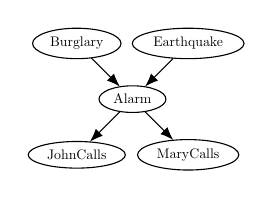
\begin{tikzpicture}[node distance=2cm,scale=0.5,every node/.style={scale=0.5}]
          \node[draw,ellipse] (alarm) {Alarm};
          \node[draw,ellipse,above left of=alarm] (burglary) {Burglary};
          \node[draw,ellipse,above right of=alarm] (earthquake) {Earthquake};
          \node[draw,ellipse,below left of=alarm] (johnCalls) {JohnCalls};
          \node[draw,ellipse,below right of=alarm] (maryCalls) {MaryCalls};
          \draw[-Latex] (burglary) -- (alarm);
          \draw[-Latex] (earthquake) -- (alarm);
          \draw[-Latex] (alarm) -- (johnCalls);
          \draw[-Latex] (alarm) -- (maryCalls);
        \end{tikzpicture}
      \end{block}
      \vspace{1cm}
      \begin{block}{Markov Random Field}
        \centering
        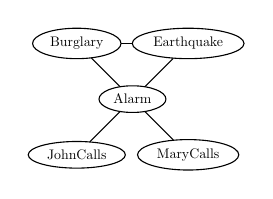
\begin{tikzpicture}[node distance=2cm,scale=0.5,every node/.style={scale=0.5}]
          \node[draw,ellipse] (alarm) {Alarm};
          \node[draw,ellipse,above left of=alarm] (burglary) {Burglary};
          \node[draw,ellipse,above right of=alarm] (earthquake) {Earthquake};
          \node[draw,ellipse,below left of=alarm] (johnCalls) {JohnCalls};
          \node[draw,ellipse,below right of=alarm] (maryCalls) {MaryCalls};
          \draw (burglary) -- (earthquake);
          \draw (burglary) -- (alarm);
          \draw (earthquake) -- (alarm);
          \draw (alarm) -- (johnCalls);
          \draw (alarm) -- (maryCalls);
        \end{tikzpicture}
      \end{block}
    \end{column}
  \end{columns}
  \onslide<2>{
    \begin{tikzpicture}[remember picture,overlay]
      \node[draw,star,fill=red!10] (wmc) at (current page.center) {WMC};
      \coordinate[xshift=-0.25\linewidth,yshift=-0.25\textheight] (p1) at (current page.center);
      \coordinate[xshift=0.25\linewidth,yshift=-0.25\textheight] (p2) at (current page.center);
      \coordinate[xshift=-0.25\linewidth,yshift=0.25\textheight] (p3) at (current page.center);
      \coordinate[xshift=0.25\linewidth,yshift=0.25\textheight] (p4) at (current page.center);
      \draw[-latex,line width=2pt,color=red!50] (p1) -- (wmc);
      \draw[-latex,line width=2pt,color=red!50] (p2) -- (wmc);
      \draw[-latex,line width=2pt,color=red!50] (p3) -- (wmc);
      \draw[-latex,line width=2pt,color=red!50] (p4) -- (wmc);
    \end{tikzpicture}
  }
\end{frame}

\begin{frame}[fragile]{Weighted Model Counting (WMC)}
  \begin{columns}
    \begin{column}{0.5\textwidth}
      \begin{itemize}
      \item Generalises propositional model counting ($\#\SAT{}$)
      \item Applications:
        \begin{itemize}
        \item graphical models
        \item probabilistic programming
        \item neural-symbolic artificial intelligence
        \end{itemize}
%      \item Main types of algorithms:
%        \begin{itemize}
%        \item using knowledge compilation
%        \item using a \SAT{} solver
%        \item manipulating pseudo-Boolean functions
%        \end{itemize}
      \end{itemize}
    \end{column}
    \begin{column}{0.5\textwidth}
      \begin{example}
      $w(x) = 0.3$, $w(\neg x) = 0.7$, $w(y) = 0.2$, $w(\neg y) = 0.8$
      \vspace{1cm}

      $\mathsf{WMC}(\alert{x \lor y}) = w(x)w(y) + w(x)w(\neg y) + w(\neg x)w(y)
      = 0.44$
      \end{example}
    \end{column}
  \end{columns}
\end{frame}

\begin{frame}{An Alternative Way to Think About WMC}
  \begin{itemize}
  \item Let \structure{$V$} be the set of variables.
  \item Then \structure{$2^{2^V}$} is the Boolean algebra of propositional
    formulas.
  \end{itemize}
  \begin{definition}
    A \alert{measure} is a function \structure{$\mu\colon 2^{2^V} \to
      \mathbb{R}_{\ge 0}$} such that:
    \begin{itemize}
    \item \structure{$\mu(\bot) = 0$};
    \item \structure{$\mu(x \lor y) = \mu(x) + \mu(y)$} whenever \structure{$x
        \land y = \bot$}.
    \end{itemize}
  \end{definition}
  \begin{block}{Observation}
    WMC corresponds to the process of calculating the value of
    \structure{$\mu(x)$} for some \structure{$x \in 2^{2^V}$}.
  \end{block}
\end{frame}

% \begin{frame}{How  to Define a Measure}
%   \begin{itemize}
%   \item A \alert{weight function} is any function \structure{$\nu\colon 2^V \to
%       \mathbb{R}_{\ge 0}$}.
%     \begin{itemize}
%     \item It is \alert{factored} if
%       \[
%         \nu = \prod_{x \in V} \nu_x
%       \]
%       for some functions \structure{$\nu_x\colon 2^{\{x\}} \to \mathbb{R}_{\ge
%           0}$}, \structure{$x \in V$}.
%     \end{itemize}
%   \item We say that \structure{$\nu$} \alert{induces} \structure{$\mu$} if
%     \[
%       \mu(x) = \sum_{\{u\} \le x} \nu(u)
%     \]
%     for all \structure{$x \in 2^{2^V}$}.
%   \item A measure \structure{$\mu$} is \alert{factorable} if there exists a
%     factored weight function \structure{$\nu$} that induces \structure{$\mu$}.
%   \end{itemize}
% \end{frame}

\begin{frame}{The Limitations and Capabilities of WMC}
  \begin{alertblock}{Observation}
    Classical WMC is only able to evaluate \structure{factorable} measures
    (c.f., a collection of mutually independent random variables).
  \end{alertblock}
  \begin{theorem}[Informal Version]
    It is always possible to add more variables to turn a non-factorable measure
    into a factorable measure.
  \end{theorem}
  However, that is not necessarily a good idea!
\end{frame}

\begin{frame}{Encoding Bayesian Networks}
  \begin{itemize}
%  \item \alert{One} variable for every random variable with \alert{two} values.
%  \item \alert{$k$} variables for every random variable with \alert{$k > 2$}
%    values.
  \item Define indicator functions of the form \structure{$[x]\colon 2^{\{x\}}
      \to \{ 0, 1 \}$}.
    \begin{itemize}
    \item \structure{$[x](\emptyset) = 0$};
    \item \structure{$[x](\{ x \}) = 1$}.
    \end{itemize}
  \item Define \structure{$+$}, \structure{$\cdot$}, and scalar multiplication pointwise.
  \item Then a conditional probability table (CPT) can be represented as a function.
  \end{itemize}
  \begin{columns}[t]
    \begin{column}{0.5\textwidth}
      \centering
      \begin{tabular}[t]{ccc}
        \toprule
        $a$ & $b$ & $\Pr(A = a \mid B = b)$ \\
        \midrule
        1 & 1 & 0.6 \\
        1 & 0 & 0.4 \\
        0 & 1 & 0.1 \\
        0 & 0 & 0.9 \\
        \bottomrule
      \end{tabular}
    \end{column}
    \begin{column}{0.5\textwidth}
      \begin{align*}
        \mathsf{CPT_A} &= 0.6[\lambda_{A=1}] \cdot [\lambda_{B=1}] \\
                       &+ 0.4[\lambda_{A=1}] \cdot \overline{[\lambda_{B=1}]} \\
                       &+ 0.1\overline{[\lambda_{A=1}]} \cdot [\lambda_{B=1}] \\
                       &+ 0.9\overline{[\lambda_{A=1}]} \cdot \overline{[\lambda_{B=1}]},
      \end{align*}
    \end{column}
  \end{columns}
\end{frame}

\begin{frame}{Experimental Results}
  \centering
  % Created by tikzDevice version 0.12.3 on 2020-08-01 17:20:52
% !TEX encoding = UTF-8 Unicode
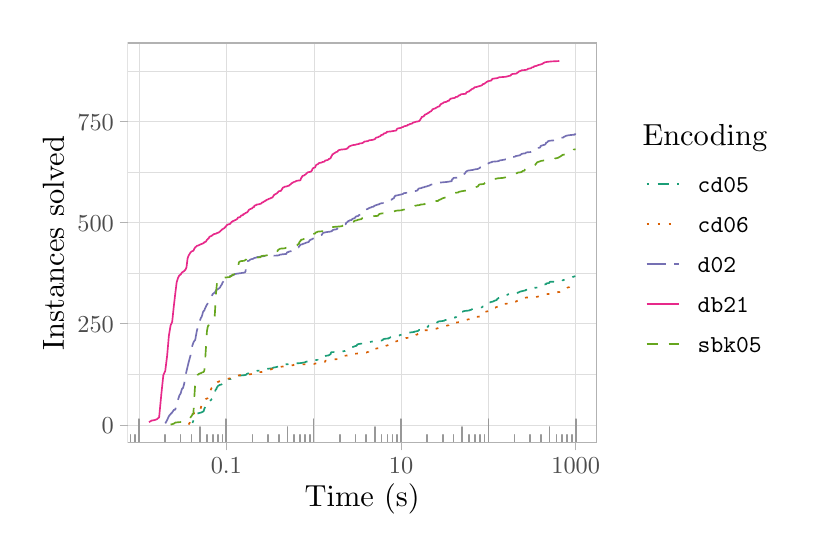
\begin{tikzpicture}[x=1pt,y=1pt]
\definecolor{fillColor}{RGB}{255,255,255}
\path[use as bounding box,fill=fillColor,fill opacity=0.00] (0,0) rectangle (278.24,180.67);
\begin{scope}
\path[clip] (  0.00,  0.00) rectangle (278.24,180.67);
\definecolor{drawColor}{RGB}{255,255,255}
\definecolor{fillColor}{RGB}{255,255,255}

\path[draw=drawColor,line width= 0.6pt,line join=round,line cap=round,fill=fillColor] (  0.00,  0.00) rectangle (278.24,180.68);
\end{scope}
\begin{scope}
\path[clip] ( 36.11, 30.69) rectangle (205.68,175.17);
\definecolor{fillColor}{RGB}{255,255,255}

\path[fill=fillColor] ( 36.11, 30.69) rectangle (205.68,175.17);
\definecolor{drawColor}{gray}{0.87}

\path[draw=drawColor,line width= 0.1pt,line join=round] ( 36.11, 55.37) --
	(205.68, 55.37);

\path[draw=drawColor,line width= 0.1pt,line join=round] ( 36.11, 91.90) --
	(205.68, 91.90);

\path[draw=drawColor,line width= 0.1pt,line join=round] ( 36.11,128.43) --
	(205.68,128.43);

\path[draw=drawColor,line width= 0.1pt,line join=round] ( 36.11,164.95) --
	(205.68,164.95);

\path[draw=drawColor,line width= 0.1pt,line join=round] ( 40.22, 30.69) --
	( 40.22,175.17);

\path[draw=drawColor,line width= 0.1pt,line join=round] (103.34, 30.69) --
	(103.34,175.17);

\path[draw=drawColor,line width= 0.1pt,line join=round] (166.47, 30.69) --
	(166.47,175.17);

\path[draw=drawColor,line width= 0.3pt,line join=round] ( 36.11, 37.11) --
	(205.68, 37.11);

\path[draw=drawColor,line width= 0.3pt,line join=round] ( 36.11, 73.64) --
	(205.68, 73.64);

\path[draw=drawColor,line width= 0.3pt,line join=round] ( 36.11,110.16) --
	(205.68,110.16);

\path[draw=drawColor,line width= 0.3pt,line join=round] ( 36.11,146.69) --
	(205.68,146.69);

\path[draw=drawColor,line width= 0.3pt,line join=round] ( 71.78, 30.69) --
	( 71.78,175.17);

\path[draw=drawColor,line width= 0.3pt,line join=round] (134.91, 30.69) --
	(134.91,175.17);

\path[draw=drawColor,line width= 0.3pt,line join=round] (198.03, 30.69) --
	(198.03,175.17);
\definecolor{drawColor}{RGB}{27,158,119}

\path[draw=drawColor,line width= 0.6pt,dash pattern=on 1pt off 3pt on 4pt off 3pt ,line join=round] ( 59.56, 37.84) --
	( 59.89, 38.71) --
	( 60.22, 39.74) --
	( 60.53, 40.47) --
	( 60.84, 40.91) --
	( 61.14, 41.20) --
	( 62.82, 41.64) --
	( 63.59, 42.08) --
	( 63.84, 42.95) --
	( 64.08, 43.54) --
	( 64.32, 44.41) --
	( 64.55, 44.85) --
	( 64.78, 45.14) --
	( 65.01, 45.29) --
	( 65.23, 45.44) --
	( 65.45, 45.58) --
	( 65.88, 45.87) --
	( 66.09, 46.02) --
	( 66.29, 46.17) --
	( 66.50, 46.46) --
	( 66.89, 46.75) --
	( 67.09, 47.34) --
	( 67.28, 47.63) --
	( 67.47, 48.07) --
	( 67.66, 48.80) --
	( 67.84, 49.67) --
	( 68.02, 49.97) --
	( 68.20, 50.11) --
	( 68.38, 50.70) --
	( 68.55, 50.84) --
	( 68.73, 51.13) --
	( 68.90, 51.28) --
	( 69.39, 51.57) --
	( 70.03, 51.72) --
	( 70.19, 51.86) --
	( 70.34, 52.01) --
	( 70.49, 52.16) --
	( 70.64, 52.60) --
	( 70.79, 52.74) --
	( 70.94, 53.03) --
	( 71.08, 53.18) --
	( 71.37, 53.33) --
	( 71.92, 53.47) --
	( 72.32, 53.62) --
	( 73.46, 53.76) --
	( 73.58, 53.91) --
	( 73.82, 54.20) --
	( 74.73, 54.35) --
	( 74.84, 54.49) --
	( 75.38, 54.64) --
	( 76.00, 54.79) --
	( 76.20, 54.93) --
	( 78.14, 55.08) --
	( 78.89, 55.23) --
	( 79.06, 55.37) --
	( 79.14, 55.52) --
	( 79.38, 55.66) --
	( 79.84, 55.81) --
	( 80.80, 55.96) --
	( 81.01, 56.10) --
	( 81.56, 56.25) --
	( 82.15, 56.39) --
	( 82.40, 56.54) --
	( 82.90, 56.69) --
	( 84.51, 56.83) --
	( 85.55, 56.98) --
	( 85.60, 57.12) --
	( 86.14, 57.27) --
	( 86.75, 57.42) --
	( 88.27, 57.56) --
	( 88.56, 57.71) --
	( 88.92, 57.86) --
	( 89.68, 58.00) --
	( 90.33, 58.15) --
	( 91.26, 58.29) --
	( 92.25, 58.44) --
	( 92.67, 58.59) --
	( 92.82, 58.73) --
	( 92.88, 58.88) --
	( 93.23, 59.02) --
	( 95.54, 59.17) --
	( 95.78, 59.32) --
	( 98.51, 59.46) --
	( 99.60, 59.61) --
	(100.18, 59.75) --
	(100.44, 59.90) --
	(100.97, 60.05) --
	(102.70, 60.19) --
	(102.77, 60.34) --
	(103.18, 60.49) --
	(104.73, 60.63) --
	(104.84, 60.78) --
	(104.86, 60.92) --
	(105.61, 61.07) --
	(105.71, 61.22) --
	(105.76, 61.36) --
	(106.49, 61.65) --
	(106.71, 61.80) --
	(107.11, 61.95) --
	(107.66, 62.09) --
	(108.70, 62.24) --
	(108.94, 62.38) --
	(109.14, 62.53) --
	(109.44, 62.68) --
	(109.53, 62.82) --
	(109.55, 62.97) --
	(109.56, 63.12) --
	(109.61, 63.26) --
	(109.79, 63.41) --
	(113.34, 63.55) --
	(113.86, 63.70) --
	(114.65, 63.85) --
	(114.85, 63.99) --
	(114.96, 64.14) --
	(115.67, 64.28) --
	(115.88, 64.43) --
	(115.93, 64.58) --
	(116.05, 64.72) --
	(116.59, 64.87) --
	(116.80, 65.01) --
	(117.01, 65.16) --
	(117.54, 65.31) --
	(117.99, 65.45) --
	(118.33, 65.60) --
	(118.91, 65.75) --
	(118.95, 65.89) --
	(119.00, 66.04) --
	(119.07, 66.18) --
	(119.49, 66.33) --
	(120.39, 66.48) --
	(122.58, 66.62) --
	(123.52, 66.77) --
	(123.65, 66.91) --
	(123.88, 67.06) --
	(124.05, 67.21) --
	(125.63, 67.35) --
	(125.97, 67.50) --
	(127.90, 67.64) --
	(128.29, 67.79) --
	(128.40, 67.94) --
	(128.51, 68.08) --
	(128.93, 68.23) --
	(130.47, 68.38) --
	(130.56, 68.52) --
	(130.91, 68.67) --
	(131.06, 68.81) --
	(132.13, 68.96) --
	(132.68, 69.11) --
	(132.88, 69.25) --
	(134.33, 69.40) --
	(134.38, 69.54) --
	(134.92, 69.69) --
	(135.51, 69.84) --
	(135.83, 69.98) --
	(136.08, 70.13) --
	(136.75, 70.27) --
	(137.17, 70.42) --
	(138.61, 70.57) --
	(139.62, 70.71) --
	(139.84, 70.86) --
	(140.77, 71.01) --
	(141.17, 71.15) --
	(141.26, 71.30) --
	(141.42, 71.44) --
	(143.11, 71.59) --
	(143.19, 71.74) --
	(143.46, 71.88) --
	(144.14, 72.03) --
	(144.34, 72.17) --
	(144.37, 72.32) --
	(144.48, 72.47) --
	(144.58, 72.61) --
	(144.79, 72.76) --
	(144.81, 72.90) --
	(144.95, 73.05) --
	(145.24, 73.20) --
	(145.47, 73.34) --
	(145.92, 73.49) --
	(147.23, 73.64) --
	(147.44, 73.78) --
	(147.46, 73.93) --
	(147.72, 74.07) --
	(148.22, 74.22) --
	(148.27, 74.37) --
	(148.30, 74.51) --
	(149.81, 74.66) --
	(150.57, 74.80) --
	(150.66, 74.95) --
	(151.33, 75.10) --
	(151.51, 75.24) --
	(151.72, 75.39) --
	(152.00, 75.53) --
	(152.11, 75.68) --
	(152.77, 75.83) --
	(154.61, 75.97) --
	(154.83, 76.12) --
	(154.90, 76.27) --
	(154.95, 76.41) --
	(155.00, 76.56) --
	(155.20, 76.70) --
	(155.26, 76.85) --
	(155.28, 77.00) --
	(155.81, 77.14) --
	(155.83, 77.29) --
	(155.95, 77.43) --
	(156.19, 77.58) --
	(156.23, 77.73) --
	(156.33, 77.87) --
	(157.14, 78.02) --
	(157.39, 78.16) --
	(158.01, 78.31) --
	(159.50, 78.46) --
	(159.73, 78.60) --
	(160.29, 78.75) --
	(160.47, 78.90) --
	(161.11, 79.04) --
	(161.73, 79.19) --
	(162.65, 79.33) --
	(163.23, 79.48) --
	(164.16, 79.63) --
	(164.29, 79.77) --
	(164.53, 79.92) --
	(165.13, 80.06) --
	(165.72, 80.21) --
	(165.75, 80.36) --
	(165.77, 80.50) --
	(166.15, 80.65) --
	(166.22, 80.79) --
	(166.27, 80.94) --
	(166.35, 81.09) --
	(166.35, 81.23) --
	(167.05, 81.38) --
	(167.35, 81.53) --
	(168.04, 81.67) --
	(168.37, 81.82) --
	(168.61, 81.96) --
	(169.05, 82.11) --
	(169.51, 82.26) --
	(169.52, 82.40) --
	(169.62, 82.55) --
	(169.80, 82.69) --
	(169.96, 82.84) --
	(170.15, 82.99) --
	(170.56, 83.13) --
	(170.65, 83.28) --
	(170.96, 83.42) --
	(171.94, 83.57) --
	(172.12, 83.72) --
	(172.36, 83.86) --
	(172.47, 84.01) --
	(173.42, 84.16) --
	(173.44, 84.30) --
	(175.96, 84.45) --
	(176.63, 84.59) --
	(176.97, 84.74) --
	(176.99, 84.89) --
	(177.55, 85.03) --
	(177.57, 85.18) --
	(178.08, 85.32) --
	(178.68, 85.47) --
	(179.32, 85.62) --
	(179.91, 85.76) --
	(180.02, 85.91) --
	(181.06, 86.05) --
	(181.14, 86.20) --
	(181.21, 86.35) --
	(182.87, 86.49) --
	(182.94, 86.64) --
	(184.41, 86.79) --
	(184.74, 86.93) --
	(184.93, 87.08) --
	(185.23, 87.22) --
	(185.27, 87.37) --
	(185.96, 87.52) --
	(186.07, 87.66) --
	(186.19, 87.81) --
	(187.31, 87.95) --
	(187.35, 88.10) --
	(187.37, 88.25) --
	(188.44, 88.39) --
	(188.53, 88.54) --
	(188.55, 88.68) --
	(188.68, 88.83) --
	(192.45, 88.98) --
	(193.20, 89.12) --
	(193.28, 89.27) --
	(193.38, 89.42) --
	(193.89, 89.56) --
	(194.14, 89.71) --
	(194.52, 89.85) --
	(195.52, 90.00) --
	(195.91, 90.15) --
	(196.52, 90.29) --
	(196.72, 90.44) --
	(196.95, 90.58) --
	(197.43, 90.73) --
	(197.91, 90.88);
\definecolor{drawColor}{RGB}{217,95,2}

\path[draw=drawColor,line width= 0.6pt,dash pattern=on 1pt off 3pt ,line join=round] ( 58.16, 37.25) --
	( 58.52, 37.84) --
	( 58.88, 39.59) --
	( 59.22, 40.47) --
	( 59.56, 41.05) --
	( 60.22, 41.34) --
	( 61.14, 41.49) --
	( 61.43, 41.78) --
	( 62.01, 41.93) --
	( 62.28, 42.08) --
	( 62.55, 43.24) --
	( 62.82, 44.27) --
	( 63.08, 44.85) --
	( 63.34, 45.44) --
	( 63.84, 45.87) --
	( 64.08, 46.02) --
	( 64.32, 46.46) --
	( 65.01, 46.75) --
	( 65.23, 46.90) --
	( 65.45, 47.34) --
	( 65.67, 47.77) --
	( 65.88, 48.65) --
	( 66.09, 49.53) --
	( 66.29, 50.11) --
	( 66.50, 50.55) --
	( 66.70, 50.84) --
	( 66.89, 51.43) --
	( 67.09, 51.57) --
	( 67.28, 51.72) --
	( 67.47, 51.86) --
	( 67.84, 52.01) --
	( 68.02, 52.16) --
	( 68.38, 52.30) --
	( 68.55, 52.60) --
	( 69.06, 52.74) --
	( 69.23, 52.89) --
	( 69.56, 53.03) --
	( 69.87, 53.18) --
	( 70.19, 53.33) --
	( 70.94, 53.47) --
	( 71.65, 53.62) --
	( 71.78, 53.76) --
	( 72.97, 53.91) --
	( 73.46, 54.06) --
	( 73.82, 54.20) --
	( 74.28, 54.49) --
	( 74.84, 54.64) --
	( 74.95, 54.79) --
	( 75.49, 54.93) --
	( 76.59, 55.08) --
	( 79.22, 55.23) --
	( 79.84, 55.37) --
	( 81.01, 55.52) --
	( 81.08, 55.66) --
	( 81.15, 55.81) --
	( 82.34, 55.96) --
	( 82.72, 56.10) --
	( 84.56, 56.25) --
	( 85.50, 56.39) --
	( 86.19, 56.54) --
	( 86.47, 56.69) --
	( 87.11, 56.83) --
	( 87.34, 56.98) --
	( 87.73, 57.12) --
	( 88.11, 57.27) --
	( 88.44, 57.42) --
	( 88.72, 57.56) --
	( 90.61, 57.86) --
	( 90.85, 58.00) --
	( 91.55, 58.15) --
	( 92.76, 58.29) --
	( 93.82, 58.44) --
	( 94.85, 58.59) --
	( 96.09, 58.73) --
	( 96.16, 58.88) --
	(100.27, 59.02) --
	(103.56, 59.17) --
	(103.99, 59.32) --
	(104.98, 59.46) --
	(105.40, 59.61) --
	(106.51, 59.75) --
	(107.46, 59.90) --
	(107.47, 60.05) --
	(107.50, 60.19) --
	(107.71, 60.34) --
	(108.64, 60.49) --
	(109.52, 60.63) --
	(110.62, 60.78) --
	(112.04, 60.92) --
	(112.14, 61.07) --
	(112.60, 61.22) --
	(112.83, 61.36) --
	(113.18, 61.51) --
	(113.48, 61.65) --
	(113.88, 61.80) --
	(114.05, 61.95) --
	(114.28, 62.09) --
	(115.62, 62.24) --
	(117.04, 62.38) --
	(117.14, 62.53) --
	(117.17, 62.68) --
	(117.61, 62.82) --
	(120.08, 62.97) --
	(120.83, 63.12) --
	(122.39, 63.26) --
	(122.72, 63.41) --
	(123.16, 63.55) --
	(123.21, 63.70) --
	(123.36, 63.85) --
	(123.36, 63.99) --
	(123.39, 64.14) --
	(123.45, 64.28) --
	(123.90, 64.43) --
	(125.26, 64.58) --
	(126.04, 64.72) --
	(126.78, 64.87) --
	(126.86, 65.01) --
	(126.88, 65.16) --
	(127.97, 65.31) --
	(128.41, 65.45) --
	(129.17, 65.60) --
	(129.56, 65.75) --
	(130.06, 65.89) --
	(130.38, 66.04) --
	(130.54, 66.18) --
	(130.85, 66.33) --
	(130.89, 66.48) --
	(131.15, 66.62) --
	(131.28, 66.77) --
	(132.02, 66.91) --
	(132.22, 67.06) --
	(132.44, 67.21) --
	(133.43, 67.35) --
	(133.58, 67.50) --
	(134.96, 67.64) --
	(135.14, 67.79) --
	(135.24, 67.94) --
	(135.48, 68.08) --
	(135.83, 68.23) --
	(136.36, 68.38) --
	(136.68, 68.52) --
	(138.14, 68.67) --
	(138.61, 68.81) --
	(139.38, 68.96) --
	(139.38, 69.11) --
	(139.57, 69.25) --
	(139.89, 69.40) --
	(140.07, 69.54) --
	(140.31, 69.69) --
	(140.91, 69.84) --
	(140.91, 69.98) --
	(141.45, 70.13) --
	(141.90, 70.27) --
	(142.10, 70.42) --
	(142.92, 70.57) --
	(143.07, 70.71) --
	(143.09, 70.86) --
	(143.28, 71.01) --
	(143.30, 71.15) --
	(143.55, 71.30) --
	(145.67, 71.44) --
	(145.79, 71.59) --
	(146.91, 71.74) --
	(147.53, 71.88) --
	(148.12, 72.03) --
	(148.43, 72.17) --
	(149.21, 72.32) --
	(149.80, 72.47) --
	(149.98, 72.61) --
	(150.56, 72.76) --
	(150.83, 72.90) --
	(151.81, 73.05) --
	(152.13, 73.20) --
	(152.20, 73.34) --
	(152.27, 73.49) --
	(152.29, 73.64) --
	(152.51, 73.78) --
	(153.79, 73.93) --
	(154.57, 74.07) --
	(155.62, 74.22) --
	(156.39, 74.37) --
	(156.92, 74.51) --
	(157.40, 74.66) --
	(157.72, 74.80) --
	(158.16, 74.95) --
	(158.71, 75.10) --
	(159.02, 75.24) --
	(160.09, 75.39) --
	(161.11, 75.53) --
	(161.61, 75.68) --
	(161.61, 75.83) --
	(161.64, 75.97) --
	(161.96, 76.12) --
	(163.07, 76.27) --
	(163.87, 76.41) --
	(164.09, 76.56) --
	(164.16, 76.70) --
	(164.19, 76.85) --
	(164.19, 77.00) --
	(164.27, 77.14) --
	(164.36, 77.29) --
	(164.37, 77.43) --
	(164.74, 77.58) --
	(164.89, 77.73) --
	(165.08, 77.87) --
	(165.27, 78.02) --
	(166.19, 78.16) --
	(166.53, 78.31) --
	(167.14, 78.46) --
	(167.22, 78.60) --
	(167.32, 78.75) --
	(167.41, 78.90) --
	(167.47, 79.04) --
	(167.60, 79.19) --
	(168.37, 79.33) --
	(168.97, 79.48) --
	(169.19, 79.63) --
	(169.60, 79.77) --
	(169.95, 79.92) --
	(170.05, 80.06) --
	(170.07, 80.21) --
	(170.29, 80.36) --
	(170.32, 80.50) --
	(171.11, 80.65) --
	(172.05, 80.79) --
	(173.03, 80.94) --
	(174.96, 81.09) --
	(175.34, 81.23) --
	(175.36, 81.38) --
	(175.59, 81.53) --
	(176.49, 81.67) --
	(176.54, 81.82) --
	(176.94, 81.96) --
	(177.77, 82.11) --
	(178.02, 82.26) --
	(178.10, 82.40) --
	(178.99, 82.55) --
	(179.08, 82.69) --
	(179.24, 82.84) --
	(179.51, 82.99) --
	(179.99, 83.13) --
	(183.14, 83.28) --
	(183.99, 83.42) --
	(184.68, 83.57) --
	(185.02, 83.72) --
	(185.75, 83.86) --
	(186.49, 84.01) --
	(186.80, 84.16) --
	(187.12, 84.30) --
	(188.18, 84.45) --
	(190.60, 84.59) --
	(190.74, 84.74) --
	(190.94, 84.89) --
	(191.10, 85.03) --
	(192.25, 85.18) --
	(192.34, 85.32) --
	(192.58, 85.47) --
	(192.67, 85.62) --
	(193.26, 85.76) --
	(193.55, 85.91) --
	(194.02, 86.05) --
	(194.49, 86.20) --
	(194.66, 86.35) --
	(194.75, 86.49) --
	(194.92, 86.64) --
	(195.22, 86.79) --
	(195.70, 86.93) --
	(195.72, 87.08) --
	(195.89, 87.22) --
	(196.24, 87.37) --
	(196.29, 87.52) --
	(196.68, 87.66);
\definecolor{drawColor}{RGB}{117,112,179}

\path[draw=drawColor,line width= 0.6pt,dash pattern=on 7pt off 3pt ,line join=round] ( 49.72, 37.69) --
	( 50.39, 38.86) --
	( 51.03, 40.32) --
	( 51.64, 41.05) --
	( 52.22, 41.64) --
	( 52.78, 42.51) --
	( 53.32, 42.66) --
	( 53.84, 44.56) --
	( 54.34, 46.31) --
	( 54.82, 47.77) --
	( 55.28, 48.50) --
	( 55.73, 50.11) --
	( 56.17, 50.55) --
	( 56.59, 52.16) --
	( 57.00, 54.93) --
	( 57.39, 56.54) --
	( 57.78, 58.15) --
	( 58.16, 59.75) --
	( 58.52, 61.07) --
	( 58.88, 62.38) --
	( 59.22, 64.87) --
	( 59.56, 65.89) --
	( 59.89, 66.91) --
	( 60.22, 67.50) --
	( 60.53, 67.79) --
	( 60.84, 69.54) --
	( 61.14, 71.15) --
	( 61.43, 72.17) --
	( 61.72, 73.49) --
	( 62.01, 74.07) --
	( 62.28, 74.95) --
	( 62.55, 75.68) --
	( 62.82, 76.12) --
	( 63.08, 76.85) --
	( 63.34, 77.87) --
	( 63.59, 78.31) --
	( 63.84, 78.46) --
	( 64.08, 79.19) --
	( 64.32, 79.63) --
	( 64.55, 80.21) --
	( 65.01, 80.94) --
	( 65.23, 81.38) --
	( 65.45, 81.82) --
	( 65.67, 82.40) --
	( 65.88, 82.84) --
	( 66.09, 83.28) --
	( 66.29, 83.57) --
	( 66.50, 83.86) --
	( 66.70, 84.01) --
	( 66.89, 84.45) --
	( 67.09, 84.59) --
	( 67.28, 84.74) --
	( 67.66, 85.03) --
	( 67.84, 85.32) --
	( 68.02, 85.76) --
	( 68.20, 85.91) --
	( 68.55, 86.05) --
	( 68.73, 86.20) --
	( 69.39, 86.64) --
	( 69.56, 86.93) --
	( 69.72, 87.22) --
	( 69.87, 87.52) --
	( 70.03, 87.66) --
	( 70.19, 87.95) --
	( 70.34, 88.39) --
	( 70.49, 88.68) --
	( 70.64, 88.83) --
	( 70.79, 89.12) --
	( 71.08, 89.27) --
	( 71.22, 89.42) --
	( 71.37, 89.85) --
	( 71.65, 90.00) --
	( 71.78, 90.15) --
	( 71.92, 90.29) --
	( 72.06, 90.44) --
	( 72.45, 90.58) --
	( 72.58, 90.73) --
	( 72.97, 90.88) --
	( 73.34, 91.02) --
	( 73.94, 91.17) --
	( 74.40, 91.31) --
	( 74.62, 91.46) --
	( 74.73, 91.61) --
	( 75.49, 91.75) --
	( 76.49, 91.90) --
	( 78.48, 92.19) --
	( 78.73, 92.63) --
	( 78.81, 93.51) --
	( 78.89, 93.80) --
	( 78.98, 94.68) --
	( 79.06, 95.26) --
	( 79.14, 95.84) --
	( 79.22, 96.14) --
	( 79.30, 96.28) --
	( 79.84, 96.43) --
	( 80.14, 96.57) --
	( 80.22, 96.72) --
	( 80.44, 96.87) --
	( 80.80, 97.01) --
	( 81.49, 97.16) --
	( 81.89, 97.45) --
	( 82.65, 97.60) --
	( 82.84, 97.74) --
	( 83.90, 97.89) --
	( 84.45, 98.04) --
	( 86.33, 98.18) --
	( 90.23, 98.33) --
	( 90.89, 98.47) --
	( 91.09, 98.62) --
	( 92.03, 98.77) --
	( 93.45, 98.91) --
	( 93.54, 99.06) --
	( 93.60, 99.20) --
	( 93.68, 99.35) --
	( 93.73, 99.50) --
	( 94.33, 99.64) --
	( 94.49, 99.79) --
	( 95.47, 99.94) --
	( 95.88,100.08) --
	( 96.14,100.23) --
	( 96.18,100.37) --
	( 96.21,100.52) --
	( 96.32,100.67) --
	( 96.39,100.81) --
	( 96.86,100.96) --
	( 97.21,101.10) --
	( 97.92,101.25) --
	( 97.96,101.54) --
	( 98.18,101.69) --
	( 98.22,101.83) --
	( 98.42,101.98) --
	( 98.46,102.13) --
	( 98.51,102.27) --
	( 99.37,102.42) --
	( 99.53,102.57) --
	(100.03,102.71) --
	(100.41,102.86) --
	(100.71,103.00) --
	(101.28,103.15) --
	(101.65,103.30) --
	(101.67,103.44) --
	(101.75,103.59) --
	(101.78,103.73) --
	(102.02,103.88) --
	(102.14,104.03) --
	(102.71,104.17) --
	(102.84,104.32) --
	(103.10,104.46) --
	(103.52,104.61) --
	(103.56,104.76) --
	(103.82,104.90) --
	(104.18,105.05) --
	(104.65,105.20) --
	(104.75,105.34) --
	(104.92,105.49) --
	(105.22,105.63) --
	(106.18,105.78) --
	(106.45,105.93) --
	(106.46,106.07) --
	(106.51,106.22) --
	(106.59,106.36) --
	(106.79,106.51) --
	(107.32,106.66) --
	(107.97,106.80) --
	(109.12,106.95) --
	(109.80,107.09) --
	(109.95,107.24) --
	(110.13,107.39) --
	(110.22,107.53) --
	(110.65,107.68) --
	(111.64,107.83) --
	(111.78,107.97) --
	(111.95,108.12) --
	(112.27,108.26) --
	(112.36,108.41) --
	(112.47,108.56) --
	(112.69,108.70) --
	(113.03,108.85) --
	(114.03,108.99) --
	(114.08,109.14) --
	(114.37,109.29) --
	(114.57,109.43) --
	(114.79,109.58) --
	(114.97,109.72) --
	(115.02,109.87) --
	(115.04,110.02) --
	(115.06,110.16) --
	(115.34,110.31) --
	(115.59,110.46) --
	(115.77,110.75) --
	(116.16,110.89) --
	(116.35,111.04) --
	(117.07,111.19) --
	(117.12,111.33) --
	(117.28,111.48) --
	(117.45,111.62) --
	(117.98,111.77) --
	(118.20,111.92) --
	(118.36,112.06) --
	(118.39,112.21) --
	(118.53,112.35) --
	(118.78,112.50) --
	(119.53,112.65) --
	(119.57,112.79) --
	(119.71,112.94) --
	(120.24,113.09) --
	(120.43,113.23) --
	(120.58,113.38) --
	(120.81,113.52) --
	(120.97,113.67) --
	(121.10,113.82) --
	(121.14,113.96) --
	(121.40,114.11) --
	(121.75,114.25) --
	(121.90,114.40) --
	(121.92,114.55) --
	(122.03,114.69) --
	(122.04,114.84) --
	(122.28,114.98) --
	(122.73,115.13) --
	(123.10,115.28) --
	(123.21,115.42) --
	(123.55,115.57) --
	(124.13,115.72) --
	(124.25,115.86) --
	(125.09,116.01) --
	(125.12,116.15) --
	(125.21,116.30) --
	(125.70,116.45) --
	(126.00,116.59) --
	(126.50,116.74) --
	(127.06,116.88) --
	(127.13,117.03) --
	(127.65,117.18) --
	(128.70,117.32) --
	(128.88,117.47) --
	(129.48,117.61) --
	(129.52,117.76) --
	(129.82,117.91) --
	(129.97,118.05) --
	(130.10,118.20) --
	(130.58,118.35) --
	(131.41,118.49) --
	(131.72,118.64) --
	(131.73,118.78) --
	(132.11,118.93) --
	(132.37,119.08) --
	(132.41,119.22) --
	(132.42,119.37) --
	(132.49,119.51) --
	(132.72,119.66) --
	(132.72,119.81) --
	(132.75,119.95) --
	(133.66,120.10) --
	(134.25,120.24) --
	(134.93,120.39) --
	(135.48,120.54) --
	(135.77,120.68) --
	(135.79,120.83) --
	(136.82,120.98) --
	(138.98,121.12) --
	(139.04,121.27) --
	(139.29,121.41) --
	(139.48,121.56) --
	(140.44,121.71) --
	(140.86,121.85) --
	(140.91,122.00) --
	(141.03,122.14) --
	(141.08,122.29) --
	(141.19,122.44) --
	(141.46,122.58) --
	(142.34,122.73) --
	(142.44,122.87) --
	(143.30,123.02) --
	(143.50,123.17) --
	(144.24,123.31) --
	(144.60,123.46) --
	(145.17,123.61) --
	(145.40,123.75) --
	(145.59,123.90) --
	(146.20,124.04) --
	(146.25,124.19) --
	(146.60,124.34) --
	(147.98,124.48) --
	(148.31,124.63) --
	(149.79,124.77) --
	(151.46,124.92) --
	(152.37,125.07) --
	(153.22,125.21) --
	(153.24,125.36) --
	(153.25,125.50) --
	(153.31,125.65) --
	(153.37,125.80) --
	(153.51,125.94) --
	(153.74,126.09) --
	(153.76,126.24) --
	(153.92,126.38) --
	(155.79,126.53) --
	(155.99,126.67) --
	(156.04,126.82) --
	(156.04,126.97) --
	(156.06,127.11) --
	(156.08,127.26) --
	(156.62,127.40) --
	(156.85,127.55) --
	(157.50,127.70) --
	(157.82,127.84) --
	(157.99,127.99) --
	(158.09,128.13) --
	(158.18,128.28) --
	(158.30,128.43) --
	(158.32,128.57) --
	(158.55,128.72) --
	(158.76,128.87) --
	(159.03,129.01) --
	(160.11,129.16) --
	(161.06,129.30) --
	(161.46,129.45) --
	(162.59,129.60) --
	(162.89,129.74) --
	(163.16,129.89) --
	(163.42,130.03) --
	(163.50,130.18) --
	(164.13,130.33) --
	(164.20,130.47) --
	(164.21,130.62) --
	(165.03,130.76) --
	(165.20,130.91) --
	(165.51,131.06) --
	(165.65,131.20) --
	(165.73,131.35) --
	(165.97,131.50) --
	(166.64,131.64) --
	(166.66,131.79) --
	(167.17,131.93) --
	(167.70,132.08) --
	(167.82,132.23) --
	(169.68,132.37) --
	(170.34,132.52) --
	(170.38,132.66) --
	(171.34,132.81) --
	(172.16,132.96) --
	(172.76,133.10) --
	(174.66,133.25) --
	(174.70,133.39) --
	(174.80,133.54) --
	(174.87,133.69) --
	(175.14,133.83) --
	(175.66,133.98) --
	(176.26,134.13) --
	(176.37,134.27) --
	(177.25,134.42) --
	(177.92,134.56) --
	(177.99,134.71) --
	(178.29,134.86) --
	(178.40,135.00) --
	(178.89,135.15) --
	(179.91,135.29) --
	(180.01,135.44) --
	(180.14,135.59) --
	(181.73,135.73) --
	(181.96,135.88) --
	(182.22,136.02) --
	(182.93,136.17) --
	(183.17,136.32) --
	(183.41,136.46) --
	(183.58,136.61) --
	(184.30,136.76) --
	(184.33,136.90) --
	(184.47,137.05) --
	(184.50,137.19) --
	(185.12,137.34) --
	(185.22,137.49) --
	(185.26,137.63) --
	(185.32,137.78) --
	(185.34,137.92) --
	(185.80,138.07) --
	(186.21,138.22) --
	(186.89,138.36) --
	(186.98,138.51) --
	(187.10,138.65) --
	(187.27,138.80) --
	(187.27,138.95) --
	(187.31,139.09) --
	(187.68,139.24) --
	(187.91,139.39) --
	(187.92,139.53) --
	(188.12,139.68) --
	(188.71,139.82) --
	(190.50,139.97) --
	(190.82,140.12) --
	(191.62,140.26) --
	(191.66,140.41) --
	(192.27,140.55) --
	(192.48,140.70) --
	(192.66,140.85) --
	(193.59,140.99) --
	(193.66,141.14) --
	(193.94,141.28) --
	(194.26,141.43) --
	(194.47,141.58) --
	(195.06,141.72) --
	(196.16,141.87) --
	(197.75,142.02) --
	(197.84,142.16) --
	(197.88,142.31) --
	(197.96,142.45);
\definecolor{drawColor}{RGB}{231,41,138}

\path[draw=drawColor,line width= 0.6pt,line join=round] ( 43.82, 38.13) --
	( 44.83, 38.71) --
	( 45.78, 38.86) --
	( 46.66, 39.15) --
	( 47.50, 39.88) --
	( 48.28, 48.07) --
	( 49.02, 55.08) --
	( 49.72, 56.69) --
	( 50.39, 62.09) --
	( 51.03, 69.40) --
	( 51.64, 73.05) --
	( 52.22, 74.37) --
	( 52.78, 79.77) --
	( 53.32, 84.45) --
	( 53.84, 88.68) --
	( 54.34, 90.29) --
	( 54.82, 91.17) --
	( 55.28, 91.46) --
	( 55.73, 92.19) --
	( 56.59, 92.78) --
	( 57.00, 93.21) --
	( 57.39, 94.09) --
	( 57.78, 97.31) --
	( 58.16, 98.33) --
	( 58.52, 98.91) --
	( 58.88, 99.50) --
	( 59.22, 99.79) --
	( 59.89,100.08) --
	( 60.22,100.81) --
	( 60.53,101.25) --
	( 60.84,101.54) --
	( 61.14,101.83) --
	( 61.72,101.98) --
	( 62.01,102.13) --
	( 62.28,102.27) --
	( 62.55,102.42) --
	( 63.08,102.57) --
	( 63.34,102.71) --
	( 63.59,102.86) --
	( 63.84,103.15) --
	( 64.32,103.30) --
	( 64.55,103.59) --
	( 64.78,104.03) --
	( 65.01,104.17) --
	( 65.23,104.46) --
	( 65.45,104.61) --
	( 65.67,105.05) --
	( 65.88,105.20) --
	( 66.29,105.34) --
	( 66.50,105.49) --
	( 66.70,105.63) --
	( 67.28,106.07) --
	( 68.02,106.22) --
	( 68.20,106.36) --
	( 68.55,106.51) --
	( 69.06,106.66) --
	( 69.39,106.95) --
	( 69.72,107.24) --
	( 69.87,107.39) --
	( 70.03,107.53) --
	( 70.19,107.68) --
	( 70.34,107.83) --
	( 70.64,107.97) --
	( 71.08,108.26) --
	( 71.22,108.41) --
	( 71.37,108.56) --
	( 71.51,108.70) --
	( 71.65,108.85) --
	( 71.92,109.29) --
	( 72.45,109.58) --
	( 73.09,109.72) --
	( 73.21,109.87) --
	( 73.34,110.02) --
	( 73.46,110.16) --
	( 73.70,110.46) --
	( 73.94,110.60) --
	( 74.05,110.75) --
	( 74.51,110.89) --
	( 74.73,111.04) --
	( 75.17,111.19) --
	( 75.38,111.33) --
	( 75.59,111.48) --
	( 75.80,111.62) --
	( 75.90,111.92) --
	( 76.00,112.06) --
	( 76.69,112.21) --
	( 76.88,112.35) --
	( 77.06,112.65) --
	( 77.16,112.79) --
	( 77.79,112.94) --
	( 77.88,113.23) --
	( 78.23,113.38) --
	( 78.56,113.52) --
	( 78.65,113.67) --
	( 79.06,113.82) --
	( 79.38,113.96) --
	( 79.45,114.11) --
	( 79.69,114.40) --
	( 79.76,114.55) --
	( 79.84,114.69) --
	( 79.92,114.84) --
	( 80.14,114.98) --
	( 80.44,115.13) --
	( 80.87,115.28) --
	( 81.15,115.42) --
	( 81.35,115.72) --
	( 81.82,115.86) --
	( 81.89,116.30) --
	( 82.21,116.45) --
	( 82.59,116.59) --
	( 82.72,116.74) --
	( 83.67,116.88) --
	( 84.12,117.03) --
	( 84.51,117.18) --
	( 84.56,117.32) --
	( 84.67,117.47) --
	( 85.14,117.61) --
	( 85.24,117.76) --
	( 85.55,117.91) --
	( 85.75,118.05) --
	( 86.09,118.20) --
	( 86.19,118.35) --
	( 86.47,118.49) --
	( 86.89,118.64) --
	( 87.07,118.78) --
	( 87.60,118.93) --
	( 87.77,119.08) --
	( 88.23,119.22) --
	( 88.40,119.37) --
	( 88.60,119.51) --
	( 88.72,119.66) --
	( 88.76,119.81) --
	( 88.84,119.95) --
	( 88.96,120.10) --
	( 89.07,120.24) --
	( 89.30,120.39) --
	( 89.57,120.54) --
	( 90.08,120.83) --
	( 90.26,120.98) --
	( 90.40,121.12) --
	( 90.54,121.41) --
	( 90.79,121.56) --
	( 91.52,121.71) --
	( 91.62,121.85) --
	( 91.68,122.00) --
	( 91.87,122.29) --
	( 92.00,122.44) --
	( 92.06,122.58) --
	( 92.25,122.87) --
	( 92.70,123.02) --
	( 92.76,123.17) --
	( 93.60,123.31) --
	( 93.98,123.46) --
	( 94.56,123.61) --
	( 94.59,123.75) --
	( 94.69,123.90) --
	( 95.05,124.04) --
	( 95.15,124.19) --
	( 95.20,124.34) --
	( 95.40,124.48) --
	( 95.83,124.63) --
	( 95.88,124.77) --
	( 96.23,124.92) --
	( 96.75,125.07) --
	( 96.92,125.21) --
	( 97.31,125.36) --
	( 98.48,125.50) --
	( 98.59,125.65) --
	( 98.69,125.94) --
	( 98.75,126.09) --
	( 98.86,126.38) --
	( 99.01,126.53) --
	( 99.05,126.67) --
	( 99.20,126.82) --
	( 99.22,126.97) --
	( 99.31,127.11) --
	( 99.85,127.26) --
	( 99.99,127.40) --
	(100.30,127.55) --
	(100.51,127.70) --
	(100.61,127.84) --
	(100.72,127.99) --
	(100.92,128.13) --
	(101.10,128.28) --
	(101.29,128.43) --
	(102.13,128.57) --
	(102.48,128.72) --
	(102.58,128.87) --
	(102.61,129.01) --
	(102.73,129.16) --
	(102.81,129.30) --
	(102.83,129.45) --
	(102.90,129.60) --
	(103.00,129.74) --
	(103.12,129.89) --
	(103.41,130.03) --
	(103.83,130.18) --
	(103.92,130.33) --
	(104.01,130.47) --
	(104.05,130.62) --
	(104.08,130.76) --
	(104.13,130.91) --
	(104.29,131.06) --
	(104.51,131.20) --
	(104.87,131.35) --
	(105.04,131.50) --
	(105.16,131.64) --
	(105.36,131.79) --
	(106.30,131.93) --
	(106.32,132.08) --
	(107.06,132.23) --
	(107.34,132.37) --
	(107.40,132.52) --
	(107.44,132.66) --
	(108.32,132.81) --
	(108.55,132.96) --
	(108.76,133.10) --
	(108.86,133.25) --
	(109.29,133.39) --
	(109.48,133.54) --
	(109.50,133.69) --
	(109.60,133.83) --
	(109.63,133.98) --
	(109.79,134.13) --
	(109.80,134.27) --
	(109.90,134.42) --
	(110.02,134.56) --
	(110.03,134.71) --
	(110.13,134.86) --
	(110.35,135.00) --
	(110.61,135.15) --
	(110.81,135.29) --
	(111.02,135.44) --
	(111.34,135.59) --
	(111.46,135.73) --
	(112.00,135.88) --
	(112.05,136.02) --
	(112.12,136.17) --
	(112.24,136.32) --
	(112.56,136.46) --
	(113.24,136.61) --
	(114.76,136.76) --
	(115.33,136.90) --
	(115.48,137.05) --
	(115.62,137.19) --
	(115.92,137.34) --
	(115.93,137.49) --
	(115.96,137.63) --
	(116.36,137.78) --
	(116.57,137.92) --
	(116.97,138.07) --
	(117.51,138.22) --
	(118.44,138.36) --
	(118.86,138.51) --
	(119.69,138.65) --
	(119.83,138.80) --
	(120.92,138.95) --
	(121.16,139.09) --
	(121.35,139.24) --
	(121.57,139.39) --
	(121.72,139.53) --
	(122.95,139.68) --
	(123.14,139.82) --
	(123.41,139.97) --
	(124.60,140.12) --
	(125.05,140.26) --
	(125.50,140.41) --
	(125.70,140.70) --
	(125.79,140.85) --
	(126.15,140.99) --
	(126.76,141.14) --
	(126.89,141.28) --
	(127.26,141.43) --
	(127.58,141.58) --
	(127.62,141.72) --
	(127.75,141.87) --
	(128.39,142.02) --
	(128.57,142.16) --
	(128.57,142.31) --
	(128.73,142.45) --
	(129.42,142.60) --
	(129.64,142.75) --
	(129.66,142.89) --
	(129.81,143.04) --
	(131.28,143.18) --
	(132.09,143.33) --
	(133.06,143.48) --
	(133.26,143.62) --
	(133.30,143.77) --
	(133.31,143.91) --
	(133.49,144.06) --
	(133.61,144.21) --
	(134.22,144.35) --
	(135.05,144.50) --
	(135.10,144.65) --
	(135.65,144.79) --
	(135.91,144.94) --
	(136.17,145.08) --
	(137.02,145.23) --
	(137.20,145.38) --
	(137.27,145.52) --
	(137.92,145.67) --
	(137.94,145.81) --
	(138.64,145.96) --
	(139.03,146.11) --
	(139.10,146.25) --
	(139.32,146.40) --
	(139.98,146.54) --
	(140.32,146.69) --
	(141.22,146.84) --
	(141.54,146.98) --
	(141.70,147.13) --
	(141.73,147.28) --
	(141.87,147.42) --
	(141.95,147.57) --
	(141.96,147.71) --
	(142.16,147.86) --
	(142.24,148.01) --
	(142.25,148.15) --
	(142.35,148.30) --
	(142.51,148.44) --
	(143.09,148.59) --
	(143.12,148.74) --
	(143.40,148.88) --
	(143.40,149.03) --
	(143.42,149.17) --
	(143.72,149.32) --
	(144.11,149.47) --
	(144.42,149.61) --
	(144.46,149.76) --
	(144.97,149.91) --
	(145.06,150.05) --
	(145.14,150.20) --
	(145.52,150.34) --
	(145.80,150.49) --
	(145.93,150.64) --
	(146.04,150.78) --
	(146.18,150.93) --
	(146.22,151.07) --
	(146.37,151.22) --
	(146.82,151.37) --
	(147.29,151.51) --
	(147.50,151.66) --
	(147.78,151.80) --
	(147.93,151.95) --
	(148.26,152.10) --
	(148.74,152.24) --
	(148.88,152.39) --
	(148.91,152.54) --
	(149.06,152.68) --
	(149.10,152.83) --
	(149.28,152.97) --
	(149.38,153.12) --
	(149.83,153.27) --
	(150.03,153.41) --
	(150.27,153.56) --
	(150.39,153.70) --
	(151.20,153.85) --
	(151.59,154.00) --
	(151.62,154.14) --
	(152.25,154.29) --
	(152.33,154.43) --
	(152.40,154.58) --
	(152.51,154.73) --
	(152.71,154.87) --
	(152.82,155.02) --
	(153.57,155.17) --
	(154.40,155.31) --
	(154.49,155.46) --
	(154.65,155.60) --
	(155.47,155.75) --
	(155.48,155.90) --
	(155.70,156.04) --
	(155.78,156.19) --
	(156.34,156.33) --
	(156.42,156.48) --
	(156.67,156.63) --
	(158.30,156.77) --
	(158.35,156.92) --
	(158.47,157.06) --
	(158.47,157.21) --
	(158.71,157.36) --
	(159.04,157.50) --
	(159.60,157.65) --
	(159.62,157.80) --
	(159.74,157.94) --
	(160.16,158.09) --
	(160.18,158.23) --
	(160.33,158.38) --
	(160.65,158.53) --
	(161.07,158.67) --
	(161.16,158.82) --
	(161.39,158.96) --
	(161.41,159.11) --
	(162.30,159.26) --
	(162.68,159.40) --
	(163.23,159.55) --
	(163.73,159.69) --
	(164.08,159.84) --
	(164.30,159.99) --
	(164.38,160.13) --
	(164.47,160.28) --
	(165.20,160.43) --
	(165.20,160.57) --
	(165.43,160.72) --
	(165.64,160.86) --
	(165.74,161.01) --
	(166.20,161.16) --
	(166.22,161.30) --
	(166.96,161.45) --
	(167.60,161.59) --
	(167.61,161.74) --
	(167.62,161.89) --
	(167.85,162.03) --
	(167.90,162.18) --
	(168.81,162.32) --
	(169.90,162.47) --
	(169.97,162.62) --
	(170.55,162.76) --
	(172.68,162.91) --
	(173.34,163.06) --
	(173.81,163.20) --
	(174.46,163.35) --
	(174.65,163.49) --
	(174.66,163.64) --
	(174.77,163.79) --
	(175.15,163.93) --
	(176.59,164.08) --
	(176.83,164.22) --
	(176.84,164.37) --
	(177.20,164.52) --
	(177.35,164.66) --
	(177.41,164.81) --
	(177.77,164.95) --
	(178.27,165.10) --
	(178.41,165.25) --
	(179.83,165.39) --
	(180.46,165.54) --
	(180.75,165.69) --
	(180.77,165.83) --
	(181.77,165.98) --
	(182.02,166.12) --
	(182.08,166.27) --
	(182.77,166.42) --
	(182.95,166.56) --
	(182.97,166.71) --
	(183.83,166.85) --
	(184.15,167.00) --
	(184.44,167.15) --
	(185.07,167.29) --
	(185.56,167.44) --
	(186.00,167.58) --
	(186.17,167.73) --
	(186.47,167.88) --
	(186.54,168.02) --
	(186.99,168.17) --
	(187.78,168.32) --
	(189.10,168.46) --
	(192.09,168.61);
\definecolor{drawColor}{RGB}{102,166,30}

\path[draw=drawColor,line width= 0.6pt,dash pattern=on 4pt off 4pt ,line join=round] ( 51.64, 37.25) --
	( 52.22, 37.40) --
	( 52.78, 37.55) --
	( 53.32, 37.98) --
	( 54.82, 38.13) --
	( 57.78, 38.28) --
	( 59.89, 41.34) --
	( 60.22, 47.19) --
	( 60.53, 51.86) --
	( 60.84, 54.49) --
	( 61.14, 54.79) --
	( 61.43, 55.23) --
	( 61.72, 55.37) --
	( 62.01, 55.66) --
	( 62.55, 55.81) --
	( 63.08, 56.10) --
	( 63.59, 56.25) --
	( 63.84, 56.83) --
	( 64.08, 59.75) --
	( 64.32, 63.55) --
	( 64.55, 66.91) --
	( 64.78, 71.01) --
	( 65.01, 72.32) --
	( 65.23, 73.05) --
	( 65.67, 73.20) --
	( 65.88, 73.34) --
	( 66.09, 73.64) --
	( 66.70, 73.78) --
	( 67.47, 75.24) --
	( 67.66, 77.58) --
	( 67.84, 81.09) --
	( 68.02, 84.16) --
	( 68.20, 86.35) --
	( 68.38, 88.10) --
	( 68.55, 88.98) --
	( 68.73, 89.12) --
	( 68.90, 89.56) --
	( 69.06, 89.71) --
	( 69.56, 90.15) --
	( 69.72, 90.29) --
	( 71.92, 90.44) --
	( 73.09, 90.58) --
	( 73.21, 90.73) --
	( 73.58, 90.88) --
	( 73.70, 91.02) --
	( 73.94, 91.31) --
	( 74.17, 91.46) --
	( 75.06, 91.61) --
	( 75.27, 91.75) --
	( 75.59, 91.90) --
	( 75.69, 92.05) --
	( 75.80, 92.19) --
	( 75.90, 93.21) --
	( 76.00, 93.80) --
	( 76.10, 94.38) --
	( 76.20, 95.11) --
	( 76.30, 95.70) --
	( 76.40, 95.99) --
	( 76.88, 96.28) --
	( 78.14, 96.43) --
	( 78.48, 96.57) --
	( 78.65, 96.72) --
	( 78.89, 96.87) --
	( 79.06, 97.01) --
	( 79.14, 97.16) --
	( 81.62, 97.31) --
	( 81.82, 97.45) --
	( 82.90, 97.60) --
	( 84.12, 97.74) --
	( 84.18, 97.89) --
	( 84.51, 98.04) --
	( 84.61, 98.18) --
	( 86.09, 98.33) --
	( 86.61, 98.47) --
	( 87.20, 98.62) --
	( 87.29, 98.91) --
	( 87.34, 99.06) --
	( 87.38, 99.20) --
	( 87.42, 99.35) --
	( 88.56, 99.50) --
	( 89.38, 99.64) --
	( 89.42, 99.79) --
	( 90.33, 99.94) --
	( 90.37,100.08) --
	( 90.44,100.23) --
	( 90.54,100.37) --
	( 90.72,100.52) --
	( 91.02,100.67) --
	( 91.22,100.81) --
	( 93.08,100.96) --
	( 93.17,101.10) --
	( 94.95,101.25) --
	( 95.93,101.40) --
	( 96.14,101.54) --
	( 96.34,101.69) --
	( 97.21,101.83) --
	( 97.40,101.98) --
	( 97.44,102.13) --
	( 97.48,102.27) --
	( 97.75,102.42) --
	( 98.00,102.57) --
	( 98.06,102.71) --
	( 98.08,103.00) --
	( 98.18,103.15) --
	( 98.42,103.44) --
	( 98.46,103.59) --
	( 98.71,103.73) --
	( 98.77,103.88) --
	( 98.78,104.03) --
	( 99.55,104.17) --
	( 99.80,104.32) --
	(100.66,104.46) --
	(100.69,104.61) --
	(100.94,104.76) --
	(100.97,104.90) --
	(100.99,105.05) --
	(101.36,105.20) --
	(101.47,105.34) --
	(101.56,105.49) --
	(101.78,105.63) --
	(102.25,105.78) --
	(102.34,105.93) --
	(102.57,106.07) --
	(103.64,106.22) --
	(103.96,106.36) --
	(103.97,106.51) --
	(104.08,106.66) --
	(104.65,106.80) --
	(104.66,106.95) --
	(106.33,107.09) --
	(108.61,107.24) --
	(108.69,107.39) --
	(108.73,107.53) --
	(108.79,107.68) --
	(108.88,107.83) --
	(108.90,107.97) --
	(108.92,108.12) --
	(109.26,108.26) --
	(109.71,108.41) --
	(109.92,108.56) --
	(110.90,108.70) --
	(112.88,108.85) --
	(113.66,108.99) --
	(113.84,109.14) --
	(114.09,109.29) --
	(114.40,109.43) --
	(114.64,109.58) --
	(114.70,109.72) --
	(114.80,109.87) --
	(115.34,110.02) --
	(115.64,110.16) --
	(116.63,110.31) --
	(117.36,110.46) --
	(117.95,110.60) --
	(117.97,110.75) --
	(118.11,110.89) --
	(118.86,111.04) --
	(119.22,111.19) --
	(119.74,111.33) --
	(120.63,111.48) --
	(120.67,111.62) --
	(120.78,111.77) --
	(121.51,111.92) --
	(123.70,112.06) --
	(123.76,112.21) --
	(123.99,112.35) --
	(124.05,112.50) --
	(126.38,112.65) --
	(126.63,112.79) --
	(126.71,112.94) --
	(126.82,113.09) --
	(126.96,113.23) --
	(127.18,113.38) --
	(127.78,113.52) --
	(129.26,113.67) --
	(129.96,113.82) --
	(130.56,113.96) --
	(130.57,114.11) --
	(132.23,114.25) --
	(132.75,114.40) --
	(133.26,114.55) --
	(135.25,114.69) --
	(135.46,114.84) --
	(136.16,114.98) --
	(136.50,115.13) --
	(137.84,115.28) --
	(137.99,115.42) --
	(138.02,115.57) --
	(138.36,115.72) --
	(138.73,115.86) --
	(139.54,116.01) --
	(139.70,116.15) --
	(139.89,116.30) --
	(140.62,116.45) --
	(141.68,116.59) --
	(141.91,116.74) --
	(143.42,116.88) --
	(143.53,117.03) --
	(143.76,117.18) --
	(143.83,117.32) --
	(143.99,117.47) --
	(144.03,117.61) --
	(145.50,117.76) --
	(145.76,117.91) --
	(148.23,118.05) --
	(148.40,118.20) --
	(148.56,118.35) --
	(148.85,118.49) --
	(149.41,118.64) --
	(149.43,118.78) --
	(149.77,118.93) --
	(150.07,119.08) --
	(150.64,119.22) --
	(151.15,119.37) --
	(151.30,119.51) --
	(151.88,119.66) --
	(151.96,119.81) --
	(152.12,119.95) --
	(152.55,120.10) --
	(153.21,120.24) --
	(153.48,120.39) --
	(153.80,120.54) --
	(153.93,120.68) --
	(154.23,120.83) --
	(154.46,120.98) --
	(155.59,121.12) --
	(155.71,121.27) --
	(156.00,121.41) --
	(156.83,121.56) --
	(157.63,121.71) --
	(158.78,121.85) --
	(159.00,122.00) --
	(159.05,122.14) --
	(159.26,122.29) --
	(159.32,122.44) --
	(159.70,122.58) --
	(159.82,122.73) --
	(160.90,122.87) --
	(161.57,123.02) --
	(162.33,123.17) --
	(162.71,123.31) --
	(162.76,123.46) --
	(162.91,123.61) --
	(162.96,123.75) --
	(163.01,123.90) --
	(163.43,124.04) --
	(164.90,124.19) --
	(164.94,124.34) --
	(165.09,124.48) --
	(165.29,124.63) --
	(165.41,124.77) --
	(165.52,124.92) --
	(166.00,125.07) --
	(166.10,125.21) --
	(167.08,125.36) --
	(167.62,125.50) --
	(167.83,125.65) --
	(167.87,125.80) --
	(168.41,125.94) --
	(169.29,126.09) --
	(169.88,126.24) --
	(171.69,126.38) --
	(172.44,126.53) --
	(172.73,126.67) --
	(173.04,126.82) --
	(173.36,126.97) --
	(173.42,127.11) --
	(174.05,127.26) --
	(174.41,127.40) --
	(174.64,127.55) --
	(175.74,127.70) --
	(175.97,127.84) --
	(176.38,127.99) --
	(176.95,128.13) --
	(176.95,128.28) --
	(178.15,128.43) --
	(178.56,128.57) --
	(178.71,128.72) --
	(178.82,128.87) --
	(179.52,129.01) --
	(179.58,129.16) --
	(179.66,129.30) --
	(179.73,129.45) --
	(179.95,129.60) --
	(180.28,129.74) --
	(180.63,129.89) --
	(181.63,130.03) --
	(181.67,130.18) --
	(182.24,130.33) --
	(182.26,130.47) --
	(182.54,130.62) --
	(182.61,130.76) --
	(183.06,130.91) --
	(183.35,131.06) --
	(183.44,131.20) --
	(183.60,131.35) --
	(183.65,131.50) --
	(183.87,131.64) --
	(183.91,131.79) --
	(184.02,131.93) --
	(184.22,132.08) --
	(184.67,132.23) --
	(185.18,132.37) --
	(185.50,132.52) --
	(186.39,132.66) --
	(188.22,132.81) --
	(188.47,132.96) --
	(189.99,133.10) --
	(190.47,133.25) --
	(190.51,133.39) --
	(191.21,133.54) --
	(191.78,133.69) --
	(191.97,133.83) --
	(192.16,133.98) --
	(192.56,134.13) --
	(192.70,134.27) --
	(192.90,134.42) --
	(193.14,134.56) --
	(193.26,134.71) --
	(194.30,134.86) --
	(194.85,135.00) --
	(195.13,135.15) --
	(195.29,135.29) --
	(196.37,135.44) --
	(196.92,135.59) --
	(196.94,135.73) --
	(196.97,135.88) --
	(197.10,136.02) --
	(197.12,136.17) --
	(197.15,136.32) --
	(197.28,136.46) --
	(197.31,136.61) --
	(197.97,136.76);
\definecolor{drawColor}{RGB}{152,152,152}

\path[draw=drawColor,line width= 0.6pt,line join=round,line cap=round] ( 37.16, 30.69) -- ( 37.16, 33.53);

\path[draw=drawColor,line width= 0.6pt,line join=round,line cap=round] ( 38.78, 30.69) -- ( 38.78, 33.53);

\path[draw=drawColor,line width= 0.6pt,line join=round,line cap=round] ( 40.22, 30.69) -- ( 40.22, 39.22);

\path[draw=drawColor,line width= 0.6pt,line join=round,line cap=round] ( 49.72, 30.69) -- ( 49.72, 33.53);

\path[draw=drawColor,line width= 0.6pt,line join=round,line cap=round] ( 55.28, 30.69) -- ( 55.28, 33.53);

\path[draw=drawColor,line width= 0.6pt,line join=round,line cap=round] ( 59.22, 30.69) -- ( 59.22, 33.53);

\path[draw=drawColor,line width= 0.6pt,line join=round,line cap=round] ( 62.28, 30.69) -- ( 62.28, 36.38);

\path[draw=drawColor,line width= 0.6pt,line join=round,line cap=round] ( 64.78, 30.69) -- ( 64.78, 33.53);

\path[draw=drawColor,line width= 0.6pt,line join=round,line cap=round] ( 66.89, 30.69) -- ( 66.89, 33.53);

\path[draw=drawColor,line width= 0.6pt,line join=round,line cap=round] ( 68.73, 30.69) -- ( 68.73, 33.53);

\path[draw=drawColor,line width= 0.6pt,line join=round,line cap=round] ( 70.34, 30.69) -- ( 70.34, 33.53);

\path[draw=drawColor,line width= 0.6pt,line join=round,line cap=round] ( 71.78, 30.69) -- ( 71.78, 39.22);

\path[draw=drawColor,line width= 0.6pt,line join=round,line cap=round] ( 81.28, 30.69) -- ( 81.28, 33.53);

\path[draw=drawColor,line width= 0.6pt,line join=round,line cap=round] ( 86.84, 30.69) -- ( 86.84, 33.53);

\path[draw=drawColor,line width= 0.6pt,line join=round,line cap=round] ( 90.79, 30.69) -- ( 90.79, 33.53);

\path[draw=drawColor,line width= 0.6pt,line join=round,line cap=round] ( 93.84, 30.69) -- ( 93.84, 36.38);

\path[draw=drawColor,line width= 0.6pt,line join=round,line cap=round] ( 96.34, 30.69) -- ( 96.34, 33.53);

\path[draw=drawColor,line width= 0.6pt,line join=round,line cap=round] ( 98.46, 30.69) -- ( 98.46, 33.53);

\path[draw=drawColor,line width= 0.6pt,line join=round,line cap=round] (100.29, 30.69) -- (100.29, 33.53);

\path[draw=drawColor,line width= 0.6pt,line join=round,line cap=round] (101.90, 30.69) -- (101.90, 33.53);

\path[draw=drawColor,line width= 0.6pt,line join=round,line cap=round] (103.34, 30.69) -- (103.34, 39.22);

\path[draw=drawColor,line width= 0.6pt,line join=round,line cap=round] (112.85, 30.69) -- (112.85, 33.53);

\path[draw=drawColor,line width= 0.6pt,line join=round,line cap=round] (118.40, 30.69) -- (118.40, 33.53);

\path[draw=drawColor,line width= 0.6pt,line join=round,line cap=round] (122.35, 30.69) -- (122.35, 33.53);

\path[draw=drawColor,line width= 0.6pt,line join=round,line cap=round] (125.41, 30.69) -- (125.41, 36.38);

\path[draw=drawColor,line width= 0.6pt,line join=round,line cap=round] (127.90, 30.69) -- (127.90, 33.53);

\path[draw=drawColor,line width= 0.6pt,line join=round,line cap=round] (130.02, 30.69) -- (130.02, 33.53);

\path[draw=drawColor,line width= 0.6pt,line join=round,line cap=round] (131.85, 30.69) -- (131.85, 33.53);

\path[draw=drawColor,line width= 0.6pt,line join=round,line cap=round] (133.46, 30.69) -- (133.46, 33.53);

\path[draw=drawColor,line width= 0.6pt,line join=round,line cap=round] (134.91, 30.69) -- (134.91, 39.22);

\path[draw=drawColor,line width= 0.6pt,line join=round,line cap=round] (144.41, 30.69) -- (144.41, 33.53);

\path[draw=drawColor,line width= 0.6pt,line join=round,line cap=round] (149.96, 30.69) -- (149.96, 33.53);

\path[draw=drawColor,line width= 0.6pt,line join=round,line cap=round] (153.91, 30.69) -- (153.91, 33.53);

\path[draw=drawColor,line width= 0.6pt,line join=round,line cap=round] (156.97, 30.69) -- (156.97, 36.38);

\path[draw=drawColor,line width= 0.6pt,line join=round,line cap=round] (159.47, 30.69) -- (159.47, 33.53);

\path[draw=drawColor,line width= 0.6pt,line join=round,line cap=round] (161.58, 30.69) -- (161.58, 33.53);

\path[draw=drawColor,line width= 0.6pt,line join=round,line cap=round] (163.41, 30.69) -- (163.41, 33.53);

\path[draw=drawColor,line width= 0.6pt,line join=round,line cap=round] (165.02, 30.69) -- (165.02, 33.53);

\path[draw=drawColor,line width= 0.6pt,line join=round,line cap=round] (166.47, 30.69) -- (166.47, 39.22);

\path[draw=drawColor,line width= 0.6pt,line join=round,line cap=round] (175.97, 30.69) -- (175.97, 33.53);

\path[draw=drawColor,line width= 0.6pt,line join=round,line cap=round] (181.53, 30.69) -- (181.53, 33.53);

\path[draw=drawColor,line width= 0.6pt,line join=round,line cap=round] (185.47, 30.69) -- (185.47, 33.53);

\path[draw=drawColor,line width= 0.6pt,line join=round,line cap=round] (188.53, 30.69) -- (188.53, 36.38);

\path[draw=drawColor,line width= 0.6pt,line join=round,line cap=round] (191.03, 30.69) -- (191.03, 33.53);

\path[draw=drawColor,line width= 0.6pt,line join=round,line cap=round] (193.14, 30.69) -- (193.14, 33.53);

\path[draw=drawColor,line width= 0.6pt,line join=round,line cap=round] (194.97, 30.69) -- (194.97, 33.53);

\path[draw=drawColor,line width= 0.6pt,line join=round,line cap=round] (196.58, 30.69) -- (196.58, 33.53);

\path[draw=drawColor,line width= 0.6pt,line join=round,line cap=round] (198.03, 30.69) -- (198.03, 39.22);
\definecolor{drawColor}{gray}{0.70}

\path[draw=drawColor,line width= 0.6pt,line join=round,line cap=round] ( 36.11, 30.69) rectangle (205.68,175.17);
\end{scope}
\begin{scope}
\path[clip] (  0.00,  0.00) rectangle (278.24,180.67);
\definecolor{drawColor}{gray}{0.30}

\node[text=drawColor,anchor=base east,inner sep=0pt, outer sep=0pt, scale=  0.88] at ( 31.16, 34.08) {0};

\node[text=drawColor,anchor=base east,inner sep=0pt, outer sep=0pt, scale=  0.88] at ( 31.16, 70.60) {250};

\node[text=drawColor,anchor=base east,inner sep=0pt, outer sep=0pt, scale=  0.88] at ( 31.16,107.13) {500};

\node[text=drawColor,anchor=base east,inner sep=0pt, outer sep=0pt, scale=  0.88] at ( 31.16,143.66) {750};
\end{scope}
\begin{scope}
\path[clip] (  0.00,  0.00) rectangle (278.24,180.67);
\definecolor{drawColor}{gray}{0.70}

\path[draw=drawColor,line width= 0.3pt,line join=round] ( 33.36, 37.11) --
	( 36.11, 37.11);

\path[draw=drawColor,line width= 0.3pt,line join=round] ( 33.36, 73.64) --
	( 36.11, 73.64);

\path[draw=drawColor,line width= 0.3pt,line join=round] ( 33.36,110.16) --
	( 36.11,110.16);

\path[draw=drawColor,line width= 0.3pt,line join=round] ( 33.36,146.69) --
	( 36.11,146.69);
\end{scope}
\begin{scope}
\path[clip] (  0.00,  0.00) rectangle (278.24,180.67);
\definecolor{drawColor}{gray}{0.70}

\path[draw=drawColor,line width= 0.3pt,line join=round] ( 71.78, 27.94) --
	( 71.78, 30.69);

\path[draw=drawColor,line width= 0.3pt,line join=round] (134.91, 27.94) --
	(134.91, 30.69);

\path[draw=drawColor,line width= 0.3pt,line join=round] (198.03, 27.94) --
	(198.03, 30.69);
\end{scope}
\begin{scope}
\path[clip] (  0.00,  0.00) rectangle (278.24,180.67);
\definecolor{drawColor}{gray}{0.30}

\node[text=drawColor,anchor=base,inner sep=0pt, outer sep=0pt, scale=  0.88] at ( 71.78, 19.68) {0.1};

\node[text=drawColor,anchor=base,inner sep=0pt, outer sep=0pt, scale=  0.88] at (134.91, 19.68) {10};

\node[text=drawColor,anchor=base,inner sep=0pt, outer sep=0pt, scale=  0.88] at (198.03, 19.68) {1000};
\end{scope}
\begin{scope}
\path[clip] (  0.00,  0.00) rectangle (278.24,180.67);
\definecolor{drawColor}{RGB}{0,0,0}

\node[text=drawColor,anchor=base,inner sep=0pt, outer sep=0pt, scale=  1.10] at (120.90,  7.64) {Time (s)};
\end{scope}
\begin{scope}
\path[clip] (  0.00,  0.00) rectangle (278.24,180.67);
\definecolor{drawColor}{RGB}{0,0,0}

\node[text=drawColor,rotate= 90.00,anchor=base,inner sep=0pt, outer sep=0pt, scale=  1.10] at ( 13.08,102.93) {Instances solved};
\end{scope}
\begin{scope}
\path[clip] (  0.00,  0.00) rectangle (278.24,180.67);
\definecolor{fillColor}{RGB}{255,255,255}

\path[fill=fillColor] (216.68, 53.69) rectangle (272.74,152.17);
\end{scope}
\begin{scope}
\path[clip] (  0.00,  0.00) rectangle (278.24,180.67);
\definecolor{drawColor}{RGB}{0,0,0}

\node[text=drawColor,anchor=base west,inner sep=0pt, outer sep=0pt, scale=  1.10] at (222.18,138.03) {Encoding};
\end{scope}
\begin{scope}
\path[clip] (  0.00,  0.00) rectangle (278.24,180.67);
\definecolor{fillColor}{RGB}{255,255,255}

\path[fill=fillColor] (222.18,117.00) rectangle (236.63,131.46);
\end{scope}
\begin{scope}
\path[clip] (  0.00,  0.00) rectangle (278.24,180.67);
\definecolor{drawColor}{RGB}{27,158,119}

\path[draw=drawColor,line width= 0.6pt,dash pattern=on 1pt off 3pt on 4pt off 3pt ,line join=round] (223.63,124.23) -- (235.19,124.23);
\end{scope}
\begin{scope}
\path[clip] (  0.00,  0.00) rectangle (278.24,180.67);
\definecolor{fillColor}{RGB}{255,255,255}

\path[fill=fillColor] (222.18,102.55) rectangle (236.63,117.00);
\end{scope}
\begin{scope}
\path[clip] (  0.00,  0.00) rectangle (278.24,180.67);
\definecolor{drawColor}{RGB}{217,95,2}

\path[draw=drawColor,line width= 0.6pt,dash pattern=on 1pt off 3pt ,line join=round] (223.63,109.78) -- (235.19,109.78);
\end{scope}
\begin{scope}
\path[clip] (  0.00,  0.00) rectangle (278.24,180.67);
\definecolor{fillColor}{RGB}{255,255,255}

\path[fill=fillColor] (222.18, 88.10) rectangle (236.63,102.55);
\end{scope}
\begin{scope}
\path[clip] (  0.00,  0.00) rectangle (278.24,180.67);
\definecolor{drawColor}{RGB}{117,112,179}

\path[draw=drawColor,line width= 0.6pt,dash pattern=on 7pt off 3pt ,line join=round] (223.63, 95.32) -- (235.19, 95.32);
\end{scope}
\begin{scope}
\path[clip] (  0.00,  0.00) rectangle (278.24,180.67);
\definecolor{fillColor}{RGB}{255,255,255}

\path[fill=fillColor] (222.18, 73.64) rectangle (236.63, 88.10);
\end{scope}
\begin{scope}
\path[clip] (  0.00,  0.00) rectangle (278.24,180.67);
\definecolor{drawColor}{RGB}{231,41,138}

\path[draw=drawColor,line width= 0.6pt,line join=round] (223.63, 80.87) -- (235.19, 80.87);
\end{scope}
\begin{scope}
\path[clip] (  0.00,  0.00) rectangle (278.24,180.67);
\definecolor{fillColor}{RGB}{255,255,255}

\path[fill=fillColor] (222.18, 59.19) rectangle (236.63, 73.64);
\end{scope}
\begin{scope}
\path[clip] (  0.00,  0.00) rectangle (278.24,180.67);
\definecolor{drawColor}{RGB}{102,166,30}

\path[draw=drawColor,line width= 0.6pt,dash pattern=on 4pt off 4pt ,line join=round] (223.63, 66.42) -- (235.19, 66.42);
\end{scope}
\begin{scope}
\path[clip] (  0.00,  0.00) rectangle (278.24,180.67);
\definecolor{drawColor}{RGB}{0,0,0}

\node[text=drawColor,anchor=base west,inner sep=0pt, outer sep=0pt, scale=  0.88] at (242.13,121.20) {\texttt{cd05}};
\end{scope}
\begin{scope}
\path[clip] (  0.00,  0.00) rectangle (278.24,180.67);
\definecolor{drawColor}{RGB}{0,0,0}

\node[text=drawColor,anchor=base west,inner sep=0pt, outer sep=0pt, scale=  0.88] at (242.13,106.75) {\texttt{cd06}};
\end{scope}
\begin{scope}
\path[clip] (  0.00,  0.00) rectangle (278.24,180.67);
\definecolor{drawColor}{RGB}{0,0,0}

\node[text=drawColor,anchor=base west,inner sep=0pt, outer sep=0pt, scale=  0.88] at (242.13, 92.29) {\texttt{d02}};
\end{scope}
\begin{scope}
\path[clip] (  0.00,  0.00) rectangle (278.24,180.67);
\definecolor{drawColor}{RGB}{0,0,0}

\node[text=drawColor,anchor=base west,inner sep=0pt, outer sep=0pt, scale=  0.88] at (242.13, 77.84) {\texttt{db21}};
\end{scope}
\begin{scope}
\path[clip] (  0.00,  0.00) rectangle (278.24,180.67);
\definecolor{drawColor}{RGB}{0,0,0}

\node[text=drawColor,anchor=base west,inner sep=0pt, outer sep=0pt, scale=  0.88] at (242.13, 63.38) {\texttt{sbk05}};
\end{scope}
\end{tikzpicture}

\end{frame}

% \begin{frame}{Compared Against the Second-Best Encoding}
%   \centering
%   % Created by tikzDevice version 0.12.3.1 on 2021-06-01 14:27:10
% !TEX encoding = UTF-8 Unicode
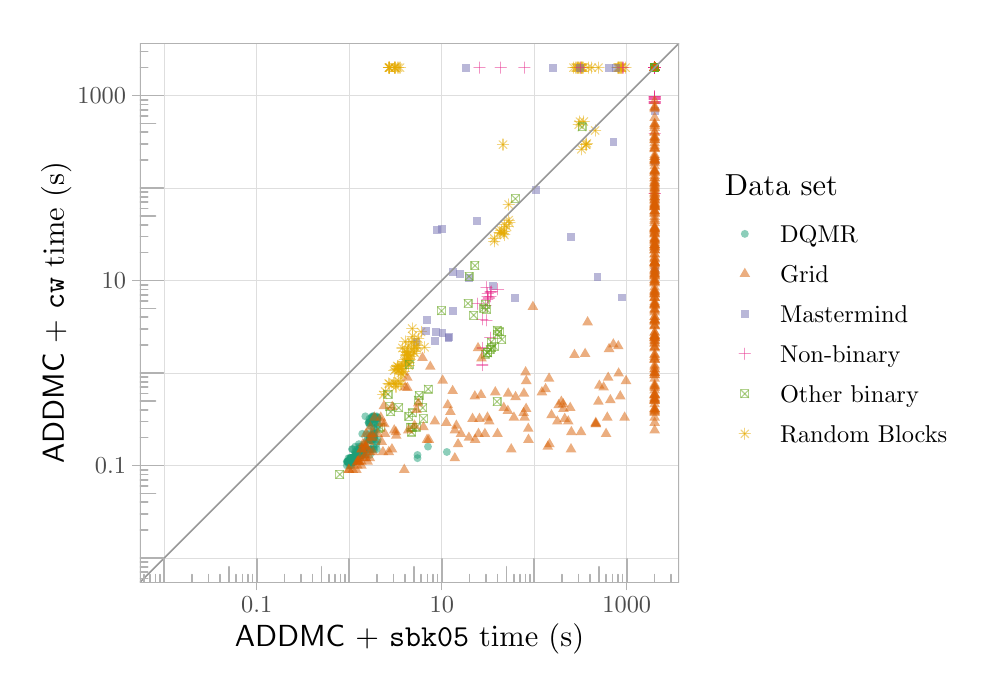
\begin{tikzpicture}[x=1pt,y=1pt]
\definecolor{fillColor}{RGB}{255,255,255}
\path[use as bounding box,fill=fillColor,fill opacity=0.00] (0,0) rectangle (343.28,231.26);
\begin{scope}
\path[clip] (  0.00,  0.09) rectangle (343.28,231.18);
\definecolor{drawColor}{RGB}{255,255,255}
\definecolor{fillColor}{RGB}{255,255,255}

\path[draw=drawColor,line width= 0.6pt,line join=round,line cap=round,fill=fillColor] (  0.00,  0.09) rectangle (343.28,231.18);
\end{scope}
\begin{scope}
\path[clip] ( 40.51, 30.77) rectangle (235.42,225.68);
\definecolor{fillColor}{RGB}{255,255,255}

\path[fill=fillColor] ( 40.51, 30.77) rectangle (235.42,225.68);
\definecolor{drawColor}{gray}{0.87}

\path[draw=drawColor,line width= 0.1pt,line join=round] ( 40.51, 39.63) --
	(235.42, 39.63);

\path[draw=drawColor,line width= 0.1pt,line join=round] ( 40.51,106.48) --
	(235.42,106.48);

\path[draw=drawColor,line width= 0.1pt,line join=round] ( 40.51,173.33) --
	(235.42,173.33);

\path[draw=drawColor,line width= 0.1pt,line join=round] ( 49.37, 30.77) --
	( 49.37,225.68);

\path[draw=drawColor,line width= 0.1pt,line join=round] (116.22, 30.77) --
	(116.22,225.68);

\path[draw=drawColor,line width= 0.1pt,line join=round] (183.07, 30.77) --
	(183.07,225.68);

\path[draw=drawColor,line width= 0.3pt,line join=round] ( 40.51, 73.06) --
	(235.42, 73.06);

\path[draw=drawColor,line width= 0.3pt,line join=round] ( 40.51,139.91) --
	(235.42,139.91);

\path[draw=drawColor,line width= 0.3pt,line join=round] ( 40.51,206.76) --
	(235.42,206.76);

\path[draw=drawColor,line width= 0.3pt,line join=round] ( 82.79, 30.77) --
	( 82.79,225.68);

\path[draw=drawColor,line width= 0.3pt,line join=round] (149.64, 30.77) --
	(149.64,225.68);

\path[draw=drawColor,line width= 0.3pt,line join=round] (216.49, 30.77) --
	(216.49,225.68);
\definecolor{drawColor}{RGB}{230,171,2}

\path[draw=drawColor,draw opacity=0.50,line width= 0.4pt,line join=round,line cap=round] (129.10,215.39) -- (131.96,218.25);

\path[draw=drawColor,draw opacity=0.50,line width= 0.4pt,line join=round,line cap=round] (129.10,218.25) -- (131.96,215.39);

\path[draw=drawColor,draw opacity=0.50,line width= 0.4pt,line join=round,line cap=round] (128.51,216.82) -- (132.55,216.82);

\path[draw=drawColor,draw opacity=0.50,line width= 0.4pt,line join=round,line cap=round] (130.53,214.80) -- (130.53,218.84);

\path[draw=drawColor,draw opacity=0.50,line width= 0.4pt,line join=round,line cap=round] (129.16,215.39) -- (132.01,218.25);

\path[draw=drawColor,draw opacity=0.50,line width= 0.4pt,line join=round,line cap=round] (129.16,218.25) -- (132.01,215.39);

\path[draw=drawColor,draw opacity=0.50,line width= 0.4pt,line join=round,line cap=round] (128.57,216.82) -- (132.60,216.82);

\path[draw=drawColor,draw opacity=0.50,line width= 0.4pt,line join=round,line cap=round] (130.58,214.80) -- (130.58,218.84);

\path[draw=drawColor,draw opacity=0.50,line width= 0.4pt,line join=round,line cap=round] (131.03,215.39) -- (133.88,218.25);

\path[draw=drawColor,draw opacity=0.50,line width= 0.4pt,line join=round,line cap=round] (131.03,218.25) -- (133.88,215.39);

\path[draw=drawColor,draw opacity=0.50,line width= 0.4pt,line join=round,line cap=round] (130.44,216.82) -- (134.47,216.82);

\path[draw=drawColor,draw opacity=0.50,line width= 0.4pt,line join=round,line cap=round] (132.45,214.80) -- (132.45,218.84);

\path[draw=drawColor,draw opacity=0.50,line width= 0.4pt,line join=round,line cap=round] (133.10,215.39) -- (135.96,218.25);

\path[draw=drawColor,draw opacity=0.50,line width= 0.4pt,line join=round,line cap=round] (133.10,218.25) -- (135.96,215.39);

\path[draw=drawColor,draw opacity=0.50,line width= 0.4pt,line join=round,line cap=round] (132.51,216.82) -- (136.55,216.82);

\path[draw=drawColor,draw opacity=0.50,line width= 0.4pt,line join=round,line cap=round] (134.53,214.80) -- (134.53,218.84);

\path[draw=drawColor,draw opacity=0.50,line width= 0.4pt,line join=round,line cap=round] (129.21,215.39) -- (132.06,218.25);

\path[draw=drawColor,draw opacity=0.50,line width= 0.4pt,line join=round,line cap=round] (129.21,218.25) -- (132.06,215.39);

\path[draw=drawColor,draw opacity=0.50,line width= 0.4pt,line join=round,line cap=round] (128.62,216.82) -- (132.66,216.82);

\path[draw=drawColor,draw opacity=0.50,line width= 0.4pt,line join=round,line cap=round] (130.64,214.80) -- (130.64,218.84);

\path[draw=drawColor,draw opacity=0.50,line width= 0.4pt,line join=round,line cap=round] (131.31,215.39) -- (134.16,218.25);

\path[draw=drawColor,draw opacity=0.50,line width= 0.4pt,line join=round,line cap=round] (131.31,218.25) -- (134.16,215.39);

\path[draw=drawColor,draw opacity=0.50,line width= 0.4pt,line join=round,line cap=round] (130.72,216.82) -- (134.75,216.82);

\path[draw=drawColor,draw opacity=0.50,line width= 0.4pt,line join=round,line cap=round] (132.74,214.80) -- (132.74,218.84);

\path[draw=drawColor,draw opacity=0.50,line width= 0.4pt,line join=round,line cap=round] (129.32,101.07) -- (132.17,103.92);

\path[draw=drawColor,draw opacity=0.50,line width= 0.4pt,line join=round,line cap=round] (129.32,103.92) -- (132.17,101.07);

\path[draw=drawColor,draw opacity=0.50,line width= 0.4pt,line join=round,line cap=round] (128.73,102.50) -- (132.76,102.50);

\path[draw=drawColor,draw opacity=0.50,line width= 0.4pt,line join=round,line cap=round] (130.75,100.48) -- (130.75,104.52);

\path[draw=drawColor,draw opacity=0.50,line width= 0.4pt,line join=round,line cap=round] (128.99,101.26) -- (131.85,104.11);

\path[draw=drawColor,draw opacity=0.50,line width= 0.4pt,line join=round,line cap=round] (128.99,104.11) -- (131.85,101.26);

\path[draw=drawColor,draw opacity=0.50,line width= 0.4pt,line join=round,line cap=round] (128.40,102.69) -- (132.44,102.69);

\path[draw=drawColor,draw opacity=0.50,line width= 0.4pt,line join=round,line cap=round] (130.42,100.67) -- (130.42,104.70);

\path[draw=drawColor,draw opacity=0.50,line width= 0.4pt,line join=round,line cap=round] (130.93,101.45) -- (133.79,104.30);

\path[draw=drawColor,draw opacity=0.50,line width= 0.4pt,line join=round,line cap=round] (130.93,104.30) -- (133.79,101.45);

\path[draw=drawColor,draw opacity=0.50,line width= 0.4pt,line join=round,line cap=round] (130.34,102.87) -- (134.38,102.87);

\path[draw=drawColor,draw opacity=0.50,line width= 0.4pt,line join=round,line cap=round] (132.36,100.86) -- (132.36,104.89);

\path[draw=drawColor,draw opacity=0.50,line width= 0.4pt,line join=round,line cap=round] (127.01, 97.15) -- (129.86,100.00);

\path[draw=drawColor,draw opacity=0.50,line width= 0.4pt,line join=round,line cap=round] (127.01,100.00) -- (129.86, 97.15);

\path[draw=drawColor,draw opacity=0.50,line width= 0.4pt,line join=round,line cap=round] (126.42, 98.57) -- (130.45, 98.57);

\path[draw=drawColor,draw opacity=0.50,line width= 0.4pt,line join=round,line cap=round] (128.44, 96.56) -- (128.44,100.59);

\path[draw=drawColor,draw opacity=0.50,line width= 0.4pt,line join=round,line cap=round] (127.80, 98.35) -- (130.65,101.20);

\path[draw=drawColor,draw opacity=0.50,line width= 0.4pt,line join=round,line cap=round] (127.80,101.20) -- (130.65, 98.35);

\path[draw=drawColor,draw opacity=0.50,line width= 0.4pt,line join=round,line cap=round] (127.21, 99.77) -- (131.25, 99.77);

\path[draw=drawColor,draw opacity=0.50,line width= 0.4pt,line join=round,line cap=round] (129.23, 97.76) -- (129.23,101.79);

\path[draw=drawColor,draw opacity=0.50,line width= 0.4pt,line join=round,line cap=round] (129.42,215.39) -- (132.28,218.25);

\path[draw=drawColor,draw opacity=0.50,line width= 0.4pt,line join=round,line cap=round] (129.42,218.25) -- (132.28,215.39);

\path[draw=drawColor,draw opacity=0.50,line width= 0.4pt,line join=round,line cap=round] (128.83,216.82) -- (132.87,216.82);

\path[draw=drawColor,draw opacity=0.50,line width= 0.4pt,line join=round,line cap=round] (130.85,214.80) -- (130.85,218.84);

\path[draw=drawColor,draw opacity=0.50,line width= 0.4pt,line join=round,line cap=round] (132.39,215.39) -- (135.24,218.25);

\path[draw=drawColor,draw opacity=0.50,line width= 0.4pt,line join=round,line cap=round] (132.39,218.25) -- (135.24,215.39);

\path[draw=drawColor,draw opacity=0.50,line width= 0.4pt,line join=round,line cap=round] (131.80,216.82) -- (135.83,216.82);

\path[draw=drawColor,draw opacity=0.50,line width= 0.4pt,line join=round,line cap=round] (133.81,214.80) -- (133.81,218.84);

\path[draw=drawColor,draw opacity=0.50,line width= 0.4pt,line join=round,line cap=round] (129.42,215.39) -- (132.28,218.25);

\path[draw=drawColor,draw opacity=0.50,line width= 0.4pt,line join=round,line cap=round] (129.42,218.25) -- (132.28,215.39);

\path[draw=drawColor,draw opacity=0.50,line width= 0.4pt,line join=round,line cap=round] (128.83,216.82) -- (132.87,216.82);

\path[draw=drawColor,draw opacity=0.50,line width= 0.4pt,line join=round,line cap=round] (130.85,214.80) -- (130.85,218.84);

\path[draw=drawColor,draw opacity=0.50,line width= 0.4pt,line join=round,line cap=round] (131.22,215.39) -- (134.07,218.25);

\path[draw=drawColor,draw opacity=0.50,line width= 0.4pt,line join=round,line cap=round] (131.22,218.25) -- (134.07,215.39);

\path[draw=drawColor,draw opacity=0.50,line width= 0.4pt,line join=round,line cap=round] (130.63,216.82) -- (134.66,216.82);

\path[draw=drawColor,draw opacity=0.50,line width= 0.4pt,line join=round,line cap=round] (132.64,214.80) -- (132.64,218.84);

\path[draw=drawColor,draw opacity=0.50,line width= 0.4pt,line join=round,line cap=round] (131.50,215.39) -- (134.35,218.25);

\path[draw=drawColor,draw opacity=0.50,line width= 0.4pt,line join=round,line cap=round] (131.50,218.25) -- (134.35,215.39);

\path[draw=drawColor,draw opacity=0.50,line width= 0.4pt,line join=round,line cap=round] (130.90,216.82) -- (134.94,216.82);

\path[draw=drawColor,draw opacity=0.50,line width= 0.4pt,line join=round,line cap=round] (132.92,214.80) -- (132.92,218.84);

\path[draw=drawColor,draw opacity=0.50,line width= 0.4pt,line join=round,line cap=round] (134.81,112.67) -- (137.66,115.53);

\path[draw=drawColor,draw opacity=0.50,line width= 0.4pt,line join=round,line cap=round] (134.81,115.53) -- (137.66,112.67);

\path[draw=drawColor,draw opacity=0.50,line width= 0.4pt,line join=round,line cap=round] (134.22,114.10) -- (138.25,114.10);

\path[draw=drawColor,draw opacity=0.50,line width= 0.4pt,line join=round,line cap=round] (136.23,112.08) -- (136.23,116.12);

\path[draw=drawColor,draw opacity=0.50,line width= 0.4pt,line join=round,line cap=round] (133.67,106.70) -- (136.52,109.55);

\path[draw=drawColor,draw opacity=0.50,line width= 0.4pt,line join=round,line cap=round] (133.67,109.55) -- (136.52,106.70);

\path[draw=drawColor,draw opacity=0.50,line width= 0.4pt,line join=round,line cap=round] (133.08,108.13) -- (137.11,108.13);

\path[draw=drawColor,draw opacity=0.50,line width= 0.4pt,line join=round,line cap=round] (135.09,106.11) -- (135.09,110.14);

\path[draw=drawColor,draw opacity=0.50,line width= 0.4pt,line join=round,line cap=round] (131.95,106.57) -- (134.80,109.42);

\path[draw=drawColor,draw opacity=0.50,line width= 0.4pt,line join=round,line cap=round] (131.95,109.42) -- (134.80,106.57);

\path[draw=drawColor,draw opacity=0.50,line width= 0.4pt,line join=round,line cap=round] (131.36,108.00) -- (135.39,108.00);

\path[draw=drawColor,draw opacity=0.50,line width= 0.4pt,line join=round,line cap=round] (133.37,105.98) -- (133.37,110.01);

\path[draw=drawColor,draw opacity=0.50,line width= 0.4pt,line join=round,line cap=round] (131.03,105.90) -- (133.88,108.75);

\path[draw=drawColor,draw opacity=0.50,line width= 0.4pt,line join=round,line cap=round] (131.03,108.75) -- (133.88,105.90);

\path[draw=drawColor,draw opacity=0.50,line width= 0.4pt,line join=round,line cap=round] (130.44,107.33) -- (134.47,107.33);

\path[draw=drawColor,draw opacity=0.50,line width= 0.4pt,line join=round,line cap=round] (132.45,105.31) -- (132.45,109.34);

\path[draw=drawColor,draw opacity=0.50,line width= 0.4pt,line join=round,line cap=round] (132.39,107.33) -- (135.24,110.19);

\path[draw=drawColor,draw opacity=0.50,line width= 0.4pt,line join=round,line cap=round] (132.39,110.19) -- (135.24,107.33);

\path[draw=drawColor,draw opacity=0.50,line width= 0.4pt,line join=round,line cap=round] (131.80,108.76) -- (135.83,108.76);

\path[draw=drawColor,draw opacity=0.50,line width= 0.4pt,line join=round,line cap=round] (133.81,106.74) -- (133.81,110.78);

\path[draw=drawColor,draw opacity=0.50,line width= 0.4pt,line join=round,line cap=round] (133.06,106.57) -- (135.91,109.42);

\path[draw=drawColor,draw opacity=0.50,line width= 0.4pt,line join=round,line cap=round] (133.06,109.42) -- (135.91,106.57);

\path[draw=drawColor,draw opacity=0.50,line width= 0.4pt,line join=round,line cap=round] (132.47,108.00) -- (136.51,108.00);

\path[draw=drawColor,draw opacity=0.50,line width= 0.4pt,line join=round,line cap=round] (134.49,105.98) -- (134.49,110.01);

\path[draw=drawColor,draw opacity=0.50,line width= 0.4pt,line join=round,line cap=round] (131.68,100.08) -- (134.53,102.94);

\path[draw=drawColor,draw opacity=0.50,line width= 0.4pt,line join=round,line cap=round] (131.68,102.94) -- (134.53,100.08);

\path[draw=drawColor,draw opacity=0.50,line width= 0.4pt,line join=round,line cap=round] (131.09,101.51) -- (135.12,101.51);

\path[draw=drawColor,draw opacity=0.50,line width= 0.4pt,line join=round,line cap=round] (133.10, 99.49) -- (133.10,103.53);

\path[draw=drawColor,draw opacity=0.50,line width= 0.4pt,line join=round,line cap=round] (133.47,101.07) -- (136.32,103.92);

\path[draw=drawColor,draw opacity=0.50,line width= 0.4pt,line join=round,line cap=round] (133.47,103.92) -- (136.32,101.07);

\path[draw=drawColor,draw opacity=0.50,line width= 0.4pt,line join=round,line cap=round] (132.88,102.50) -- (136.91,102.50);

\path[draw=drawColor,draw opacity=0.50,line width= 0.4pt,line join=round,line cap=round] (134.89,100.48) -- (134.89,104.52);

\path[draw=drawColor,draw opacity=0.50,line width= 0.4pt,line join=round,line cap=round] (131.36,101.07) -- (134.21,103.92);

\path[draw=drawColor,draw opacity=0.50,line width= 0.4pt,line join=round,line cap=round] (131.36,103.92) -- (134.21,101.07);

\path[draw=drawColor,draw opacity=0.50,line width= 0.4pt,line join=round,line cap=round] (130.77,102.50) -- (134.80,102.50);

\path[draw=drawColor,draw opacity=0.50,line width= 0.4pt,line join=round,line cap=round] (132.78,100.48) -- (132.78,104.52);

\path[draw=drawColor,draw opacity=0.50,line width= 0.4pt,line join=round,line cap=round] (134.06,104.46) -- (136.91,107.32);

\path[draw=drawColor,draw opacity=0.50,line width= 0.4pt,line join=round,line cap=round] (134.06,107.32) -- (136.91,104.46);

\path[draw=drawColor,draw opacity=0.50,line width= 0.4pt,line join=round,line cap=round] (133.47,105.89) -- (137.50,105.89);

\path[draw=drawColor,draw opacity=0.50,line width= 0.4pt,line join=round,line cap=round] (135.48,103.87) -- (135.48,107.91);

\path[draw=drawColor,draw opacity=0.50,line width= 0.4pt,line join=round,line cap=round] (132.56,102.17) -- (135.41,105.03);

\path[draw=drawColor,draw opacity=0.50,line width= 0.4pt,line join=round,line cap=round] (132.56,105.03) -- (135.41,102.17);

\path[draw=drawColor,draw opacity=0.50,line width= 0.4pt,line join=round,line cap=round] (131.97,103.60) -- (136.00,103.60);

\path[draw=drawColor,draw opacity=0.50,line width= 0.4pt,line join=round,line cap=round] (133.98,101.58) -- (133.98,105.62);

\path[draw=drawColor,draw opacity=0.50,line width= 0.4pt,line join=round,line cap=round] (132.52,106.17) -- (135.37,109.03);

\path[draw=drawColor,draw opacity=0.50,line width= 0.4pt,line join=round,line cap=round] (132.52,109.03) -- (135.37,106.17);

\path[draw=drawColor,draw opacity=0.50,line width= 0.4pt,line join=round,line cap=round] (131.92,107.60) -- (135.96,107.60);

\path[draw=drawColor,draw opacity=0.50,line width= 0.4pt,line join=round,line cap=round] (133.94,105.58) -- (133.94,109.62);

\path[draw=drawColor,draw opacity=0.50,line width= 0.4pt,line join=round,line cap=round] (131.45,106.44) -- (134.30,109.29);

\path[draw=drawColor,draw opacity=0.50,line width= 0.4pt,line join=round,line cap=round] (131.45,109.29) -- (134.30,106.44);

\path[draw=drawColor,draw opacity=0.50,line width= 0.4pt,line join=round,line cap=round] (130.86,107.86) -- (134.89,107.86);

\path[draw=drawColor,draw opacity=0.50,line width= 0.4pt,line join=round,line cap=round] (132.88,105.85) -- (132.88,109.88);

\path[draw=drawColor,draw opacity=0.50,line width= 0.4pt,line join=round,line cap=round] (134.02,107.94) -- (136.87,110.79);

\path[draw=drawColor,draw opacity=0.50,line width= 0.4pt,line join=round,line cap=round] (134.02,110.79) -- (136.87,107.94);

\path[draw=drawColor,draw opacity=0.50,line width= 0.4pt,line join=round,line cap=round] (133.43,109.37) -- (137.46,109.37);

\path[draw=drawColor,draw opacity=0.50,line width= 0.4pt,line join=round,line cap=round] (135.45,107.35) -- (135.45,111.39);

\path[draw=drawColor,draw opacity=0.50,line width= 0.4pt,line join=round,line cap=round] (132.08,107.58) -- (134.93,110.43);

\path[draw=drawColor,draw opacity=0.50,line width= 0.4pt,line join=round,line cap=round] (132.08,110.43) -- (134.93,107.58);

\path[draw=drawColor,draw opacity=0.50,line width= 0.4pt,line join=round,line cap=round] (131.49,109.01) -- (135.52,109.01);

\path[draw=drawColor,draw opacity=0.50,line width= 0.4pt,line join=round,line cap=round] (133.51,106.99) -- (133.51,111.02);

\path[draw=drawColor,draw opacity=0.50,line width= 0.4pt,line join=round,line cap=round] (133.63,107.33) -- (136.48,110.19);

\path[draw=drawColor,draw opacity=0.50,line width= 0.4pt,line join=round,line cap=round] (133.63,110.19) -- (136.48,107.33);

\path[draw=drawColor,draw opacity=0.50,line width= 0.4pt,line join=round,line cap=round] (133.04,108.76) -- (137.07,108.76);

\path[draw=drawColor,draw opacity=0.50,line width= 0.4pt,line join=round,line cap=round] (135.05,106.74) -- (135.05,110.78);

\path[draw=drawColor,draw opacity=0.50,line width= 0.4pt,line join=round,line cap=round] (138.47,112.24) -- (141.33,115.09);

\path[draw=drawColor,draw opacity=0.50,line width= 0.4pt,line join=round,line cap=round] (138.47,115.09) -- (141.33,112.24);

\path[draw=drawColor,draw opacity=0.50,line width= 0.4pt,line join=round,line cap=round] (137.88,113.66) -- (141.92,113.66);

\path[draw=drawColor,draw opacity=0.50,line width= 0.4pt,line join=round,line cap=round] (139.90,111.64) -- (139.90,115.68);

\path[draw=drawColor,draw opacity=0.50,line width= 0.4pt,line join=round,line cap=round] (136.91,111.04) -- (139.77,113.89);

\path[draw=drawColor,draw opacity=0.50,line width= 0.4pt,line join=round,line cap=round] (136.91,113.89) -- (139.77,111.04);

\path[draw=drawColor,draw opacity=0.50,line width= 0.4pt,line join=round,line cap=round] (136.32,112.46) -- (140.36,112.46);

\path[draw=drawColor,draw opacity=0.50,line width= 0.4pt,line join=round,line cap=round] (138.34,110.45) -- (138.34,114.48);

\path[draw=drawColor,draw opacity=0.50,line width= 0.4pt,line join=round,line cap=round] (136.10,114.75) -- (138.95,117.60);

\path[draw=drawColor,draw opacity=0.50,line width= 0.4pt,line join=round,line cap=round] (136.10,117.60) -- (138.95,114.75);

\path[draw=drawColor,draw opacity=0.50,line width= 0.4pt,line join=round,line cap=round] (135.51,116.18) -- (139.55,116.18);

\path[draw=drawColor,draw opacity=0.50,line width= 0.4pt,line join=round,line cap=round] (137.53,114.16) -- (137.53,118.19);

\path[draw=drawColor,draw opacity=0.50,line width= 0.4pt,line join=round,line cap=round] (138.13,112.67) -- (140.98,115.53);

\path[draw=drawColor,draw opacity=0.50,line width= 0.4pt,line join=round,line cap=round] (138.13,115.53) -- (140.98,112.67);

\path[draw=drawColor,draw opacity=0.50,line width= 0.4pt,line join=round,line cap=round] (137.54,114.10) -- (141.57,114.10);

\path[draw=drawColor,draw opacity=0.50,line width= 0.4pt,line join=round,line cap=round] (139.55,112.08) -- (139.55,116.12);

\path[draw=drawColor,draw opacity=0.50,line width= 0.4pt,line join=round,line cap=round] (138.39,116.50) -- (141.24,119.35);

\path[draw=drawColor,draw opacity=0.50,line width= 0.4pt,line join=round,line cap=round] (138.39,119.35) -- (141.24,116.50);

\path[draw=drawColor,draw opacity=0.50,line width= 0.4pt,line join=round,line cap=round] (137.80,117.93) -- (141.83,117.93);

\path[draw=drawColor,draw opacity=0.50,line width= 0.4pt,line join=round,line cap=round] (139.81,115.91) -- (139.81,119.94);

\path[draw=drawColor,draw opacity=0.50,line width= 0.4pt,line join=round,line cap=round] (135.83,111.42) -- (138.68,114.27);

\path[draw=drawColor,draw opacity=0.50,line width= 0.4pt,line join=round,line cap=round] (135.83,114.27) -- (138.68,111.42);

\path[draw=drawColor,draw opacity=0.50,line width= 0.4pt,line join=round,line cap=round] (135.24,112.84) -- (139.28,112.84);

\path[draw=drawColor,draw opacity=0.50,line width= 0.4pt,line join=round,line cap=round] (137.26,110.83) -- (137.26,114.86);

\path[draw=drawColor,draw opacity=0.50,line width= 0.4pt,line join=round,line cap=round] (135.42,111.60) -- (138.27,114.46);

\path[draw=drawColor,draw opacity=0.50,line width= 0.4pt,line join=round,line cap=round] (135.42,114.46) -- (138.27,111.60);

\path[draw=drawColor,draw opacity=0.50,line width= 0.4pt,line join=round,line cap=round] (134.83,113.03) -- (138.86,113.03);

\path[draw=drawColor,draw opacity=0.50,line width= 0.4pt,line join=round,line cap=round] (136.84,111.01) -- (136.84,115.05);

\path[draw=drawColor,draw opacity=0.50,line width= 0.4pt,line join=round,line cap=round] (133.47,105.05) -- (136.32,107.91);

\path[draw=drawColor,draw opacity=0.50,line width= 0.4pt,line join=round,line cap=round] (133.47,107.91) -- (136.32,105.05);

\path[draw=drawColor,draw opacity=0.50,line width= 0.4pt,line join=round,line cap=round] (132.88,106.48) -- (136.91,106.48);

\path[draw=drawColor,draw opacity=0.50,line width= 0.4pt,line join=round,line cap=round] (134.89,104.46) -- (134.89,108.50);

\path[draw=drawColor,draw opacity=0.50,line width= 0.4pt,line join=round,line cap=round] (136.27,107.70) -- (139.12,110.55);

\path[draw=drawColor,draw opacity=0.50,line width= 0.4pt,line join=round,line cap=round] (136.27,110.55) -- (139.12,107.70);

\path[draw=drawColor,draw opacity=0.50,line width= 0.4pt,line join=round,line cap=round] (135.68,109.13) -- (139.71,109.13);

\path[draw=drawColor,draw opacity=0.50,line width= 0.4pt,line join=round,line cap=round] (137.69,107.11) -- (137.69,111.15);

\path[draw=drawColor,draw opacity=0.50,line width= 0.4pt,line join=round,line cap=round] (135.73,112.59) -- (138.58,115.44);

\path[draw=drawColor,draw opacity=0.50,line width= 0.4pt,line join=round,line cap=round] (135.73,115.44) -- (138.58,112.59);

\path[draw=drawColor,draw opacity=0.50,line width= 0.4pt,line join=round,line cap=round] (135.14,114.01) -- (139.17,114.01);

\path[draw=drawColor,draw opacity=0.50,line width= 0.4pt,line join=round,line cap=round] (137.16,111.99) -- (137.16,116.03);

\path[draw=drawColor,draw opacity=0.50,line width= 0.4pt,line join=round,line cap=round] (134.47,105.48) -- (137.33,108.34);

\path[draw=drawColor,draw opacity=0.50,line width= 0.4pt,line join=round,line cap=round] (134.47,108.34) -- (137.33,105.48);

\path[draw=drawColor,draw opacity=0.50,line width= 0.4pt,line join=round,line cap=round] (133.88,106.91) -- (137.92,106.91);

\path[draw=drawColor,draw opacity=0.50,line width= 0.4pt,line join=round,line cap=round] (135.90,104.89) -- (135.90,108.93);

\path[draw=drawColor,draw opacity=0.50,line width= 0.4pt,line join=round,line cap=round] (137.53,121.10) -- (140.39,123.95);

\path[draw=drawColor,draw opacity=0.50,line width= 0.4pt,line join=round,line cap=round] (137.53,123.95) -- (140.39,121.10);

\path[draw=drawColor,draw opacity=0.50,line width= 0.4pt,line join=round,line cap=round] (136.94,122.53) -- (140.98,122.53);

\path[draw=drawColor,draw opacity=0.50,line width= 0.4pt,line join=round,line cap=round] (138.96,120.51) -- (138.96,124.54);

\path[draw=drawColor,draw opacity=0.50,line width= 0.4pt,line join=round,line cap=round] (134.95,116.43) -- (137.81,119.29);

\path[draw=drawColor,draw opacity=0.50,line width= 0.4pt,line join=round,line cap=round] (134.95,119.29) -- (137.81,116.43);

\path[draw=drawColor,draw opacity=0.50,line width= 0.4pt,line join=round,line cap=round] (134.36,117.86) -- (138.40,117.86);

\path[draw=drawColor,draw opacity=0.50,line width= 0.4pt,line join=round,line cap=round] (136.38,115.84) -- (136.38,119.88);

\path[draw=drawColor,draw opacity=0.50,line width= 0.4pt,line join=round,line cap=round] (134.84,109.84) -- (137.70,112.69);

\path[draw=drawColor,draw opacity=0.50,line width= 0.4pt,line join=round,line cap=round] (134.84,112.69) -- (137.70,109.84);

\path[draw=drawColor,draw opacity=0.50,line width= 0.4pt,line join=round,line cap=round] (134.25,111.26) -- (138.29,111.26);

\path[draw=drawColor,draw opacity=0.50,line width= 0.4pt,line join=round,line cap=round] (136.27,109.24) -- (136.27,113.28);

\path[draw=drawColor,draw opacity=0.50,line width= 0.4pt,line join=round,line cap=round] (134.73,109.19) -- (137.59,112.05);

\path[draw=drawColor,draw opacity=0.50,line width= 0.4pt,line join=round,line cap=round] (134.73,112.05) -- (137.59,109.19);

\path[draw=drawColor,draw opacity=0.50,line width= 0.4pt,line join=round,line cap=round] (134.14,110.62) -- (138.18,110.62);

\path[draw=drawColor,draw opacity=0.50,line width= 0.4pt,line join=round,line cap=round] (136.16,108.60) -- (136.16,112.64);

\path[draw=drawColor,draw opacity=0.50,line width= 0.4pt,line join=round,line cap=round] (135.97,111.23) -- (138.82,114.08);

\path[draw=drawColor,draw opacity=0.50,line width= 0.4pt,line join=round,line cap=round] (135.97,114.08) -- (138.82,111.23);

\path[draw=drawColor,draw opacity=0.50,line width= 0.4pt,line join=round,line cap=round] (135.38,112.65) -- (139.41,112.65);

\path[draw=drawColor,draw opacity=0.50,line width= 0.4pt,line join=round,line cap=round] (137.39,110.64) -- (137.39,114.67);

\path[draw=drawColor,draw opacity=0.50,line width= 0.4pt,line join=round,line cap=round] (225.13,215.39) -- (227.98,218.25);

\path[draw=drawColor,draw opacity=0.50,line width= 0.4pt,line join=round,line cap=round] (225.13,218.25) -- (227.98,215.39);

\path[draw=drawColor,draw opacity=0.50,line width= 0.4pt,line join=round,line cap=round] (224.54,216.82) -- (228.57,216.82);

\path[draw=drawColor,draw opacity=0.50,line width= 0.4pt,line join=round,line cap=round] (226.56,214.80) -- (226.56,218.84);

\path[draw=drawColor,draw opacity=0.50,line width= 0.4pt,line join=round,line cap=round] (225.13,215.39) -- (227.98,218.25);

\path[draw=drawColor,draw opacity=0.50,line width= 0.4pt,line join=round,line cap=round] (225.13,218.25) -- (227.98,215.39);

\path[draw=drawColor,draw opacity=0.50,line width= 0.4pt,line join=round,line cap=round] (224.54,216.82) -- (228.57,216.82);

\path[draw=drawColor,draw opacity=0.50,line width= 0.4pt,line join=round,line cap=round] (226.56,214.80) -- (226.56,218.84);

\path[draw=drawColor,draw opacity=0.50,line width= 0.4pt,line join=round,line cap=round] (225.13,215.39) -- (227.98,218.25);

\path[draw=drawColor,draw opacity=0.50,line width= 0.4pt,line join=round,line cap=round] (225.13,218.25) -- (227.98,215.39);

\path[draw=drawColor,draw opacity=0.50,line width= 0.4pt,line join=round,line cap=round] (224.54,216.82) -- (228.57,216.82);

\path[draw=drawColor,draw opacity=0.50,line width= 0.4pt,line join=round,line cap=round] (226.56,214.80) -- (226.56,218.84);

\path[draw=drawColor,draw opacity=0.50,line width= 0.4pt,line join=round,line cap=round] (225.13,215.39) -- (227.98,218.25);

\path[draw=drawColor,draw opacity=0.50,line width= 0.4pt,line join=round,line cap=round] (225.13,218.25) -- (227.98,215.39);

\path[draw=drawColor,draw opacity=0.50,line width= 0.4pt,line join=round,line cap=round] (224.54,216.82) -- (228.57,216.82);

\path[draw=drawColor,draw opacity=0.50,line width= 0.4pt,line join=round,line cap=round] (226.56,214.80) -- (226.56,218.84);

\path[draw=drawColor,draw opacity=0.50,line width= 0.4pt,line join=round,line cap=round] (225.13,215.39) -- (227.98,218.25);

\path[draw=drawColor,draw opacity=0.50,line width= 0.4pt,line join=round,line cap=round] (225.13,218.25) -- (227.98,215.39);

\path[draw=drawColor,draw opacity=0.50,line width= 0.4pt,line join=round,line cap=round] (224.54,216.82) -- (228.57,216.82);

\path[draw=drawColor,draw opacity=0.50,line width= 0.4pt,line join=round,line cap=round] (226.56,214.80) -- (226.56,218.84);

\path[draw=drawColor,draw opacity=0.50,line width= 0.4pt,line join=round,line cap=round] (225.13,215.39) -- (227.98,218.25);

\path[draw=drawColor,draw opacity=0.50,line width= 0.4pt,line join=round,line cap=round] (225.13,218.25) -- (227.98,215.39);

\path[draw=drawColor,draw opacity=0.50,line width= 0.4pt,line join=round,line cap=round] (224.54,216.82) -- (228.57,216.82);

\path[draw=drawColor,draw opacity=0.50,line width= 0.4pt,line join=round,line cap=round] (226.56,214.80) -- (226.56,218.84);

\path[draw=drawColor,draw opacity=0.50,line width= 0.4pt,line join=round,line cap=round] (170.33,187.58) -- (173.18,190.43);

\path[draw=drawColor,draw opacity=0.50,line width= 0.4pt,line join=round,line cap=round] (170.33,190.43) -- (173.18,187.58);

\path[draw=drawColor,draw opacity=0.50,line width= 0.4pt,line join=round,line cap=round] (169.74,189.01) -- (173.77,189.01);

\path[draw=drawColor,draw opacity=0.50,line width= 0.4pt,line join=round,line cap=round] (171.76,186.99) -- (171.76,191.02);

\path[draw=drawColor,draw opacity=0.50,line width= 0.4pt,line join=round,line cap=round] (169.07,155.90) -- (171.93,158.76);

\path[draw=drawColor,draw opacity=0.50,line width= 0.4pt,line join=round,line cap=round] (169.07,158.76) -- (171.93,155.90);

\path[draw=drawColor,draw opacity=0.50,line width= 0.4pt,line join=round,line cap=round] (168.48,157.33) -- (172.52,157.33);

\path[draw=drawColor,draw opacity=0.50,line width= 0.4pt,line join=round,line cap=round] (170.50,155.31) -- (170.50,159.35);

\path[draw=drawColor,draw opacity=0.50,line width= 0.4pt,line join=round,line cap=round] (167.16,152.68) -- (170.01,155.53);

\path[draw=drawColor,draw opacity=0.50,line width= 0.4pt,line join=round,line cap=round] (167.16,155.53) -- (170.01,152.68);

\path[draw=drawColor,draw opacity=0.50,line width= 0.4pt,line join=round,line cap=round] (166.57,154.11) -- (170.60,154.11);

\path[draw=drawColor,draw opacity=0.50,line width= 0.4pt,line join=round,line cap=round] (168.59,152.09) -- (168.59,156.13);

\path[draw=drawColor,draw opacity=0.50,line width= 0.4pt,line join=round,line cap=round] (170.77,156.31) -- (173.62,159.16);

\path[draw=drawColor,draw opacity=0.50,line width= 0.4pt,line join=round,line cap=round] (170.77,159.16) -- (173.62,156.31);

\path[draw=drawColor,draw opacity=0.50,line width= 0.4pt,line join=round,line cap=round] (170.18,157.74) -- (174.21,157.74);

\path[draw=drawColor,draw opacity=0.50,line width= 0.4pt,line join=round,line cap=round] (172.19,155.72) -- (172.19,159.75);

\path[draw=drawColor,draw opacity=0.50,line width= 0.4pt,line join=round,line cap=round] (167.12,153.70) -- (169.98,156.55);

\path[draw=drawColor,draw opacity=0.50,line width= 0.4pt,line join=round,line cap=round] (167.12,156.55) -- (169.98,153.70);

\path[draw=drawColor,draw opacity=0.50,line width= 0.4pt,line join=round,line cap=round] (166.53,155.12) -- (170.57,155.12);

\path[draw=drawColor,draw opacity=0.50,line width= 0.4pt,line join=round,line cap=round] (168.55,153.11) -- (168.55,157.14);

\path[draw=drawColor,draw opacity=0.50,line width= 0.4pt,line join=round,line cap=round] (225.13,215.39) -- (227.98,218.25);

\path[draw=drawColor,draw opacity=0.50,line width= 0.4pt,line join=round,line cap=round] (225.13,218.25) -- (227.98,215.39);

\path[draw=drawColor,draw opacity=0.50,line width= 0.4pt,line join=round,line cap=round] (224.54,216.82) -- (228.57,216.82);

\path[draw=drawColor,draw opacity=0.50,line width= 0.4pt,line join=round,line cap=round] (226.56,214.80) -- (226.56,218.84);

\path[draw=drawColor,draw opacity=0.50,line width= 0.4pt,line join=round,line cap=round] (225.13,215.39) -- (227.98,218.25);

\path[draw=drawColor,draw opacity=0.50,line width= 0.4pt,line join=round,line cap=round] (225.13,218.25) -- (227.98,215.39);

\path[draw=drawColor,draw opacity=0.50,line width= 0.4pt,line join=round,line cap=round] (224.54,216.82) -- (228.57,216.82);

\path[draw=drawColor,draw opacity=0.50,line width= 0.4pt,line join=round,line cap=round] (226.56,214.80) -- (226.56,218.84);

\path[draw=drawColor,draw opacity=0.50,line width= 0.4pt,line join=round,line cap=round] (225.13,215.39) -- (227.98,218.25);

\path[draw=drawColor,draw opacity=0.50,line width= 0.4pt,line join=round,line cap=round] (225.13,218.25) -- (227.98,215.39);

\path[draw=drawColor,draw opacity=0.50,line width= 0.4pt,line join=round,line cap=round] (224.54,216.82) -- (228.57,216.82);

\path[draw=drawColor,draw opacity=0.50,line width= 0.4pt,line join=round,line cap=round] (226.56,214.80) -- (226.56,218.84);

\path[draw=drawColor,draw opacity=0.50,line width= 0.4pt,line join=round,line cap=round] (225.13,215.39) -- (227.98,218.25);

\path[draw=drawColor,draw opacity=0.50,line width= 0.4pt,line join=round,line cap=round] (225.13,218.25) -- (227.98,215.39);

\path[draw=drawColor,draw opacity=0.50,line width= 0.4pt,line join=round,line cap=round] (224.54,216.82) -- (228.57,216.82);

\path[draw=drawColor,draw opacity=0.50,line width= 0.4pt,line join=round,line cap=round] (226.56,214.80) -- (226.56,218.84);

\path[draw=drawColor,draw opacity=0.50,line width= 0.4pt,line join=round,line cap=round] (225.13,215.39) -- (227.98,218.25);

\path[draw=drawColor,draw opacity=0.50,line width= 0.4pt,line join=round,line cap=round] (225.13,218.25) -- (227.98,215.39);

\path[draw=drawColor,draw opacity=0.50,line width= 0.4pt,line join=round,line cap=round] (224.54,216.82) -- (228.57,216.82);

\path[draw=drawColor,draw opacity=0.50,line width= 0.4pt,line join=round,line cap=round] (226.56,214.80) -- (226.56,218.84);

\path[draw=drawColor,draw opacity=0.50,line width= 0.4pt,line join=round,line cap=round] (198.59,215.39) -- (201.44,218.25);

\path[draw=drawColor,draw opacity=0.50,line width= 0.4pt,line join=round,line cap=round] (198.59,218.25) -- (201.44,215.39);

\path[draw=drawColor,draw opacity=0.50,line width= 0.4pt,line join=round,line cap=round] (198.00,216.82) -- (202.04,216.82);

\path[draw=drawColor,draw opacity=0.50,line width= 0.4pt,line join=round,line cap=round] (200.02,214.80) -- (200.02,218.84);

\path[draw=drawColor,draw opacity=0.50,line width= 0.4pt,line join=round,line cap=round] (198.49,215.39) -- (201.34,218.25);

\path[draw=drawColor,draw opacity=0.50,line width= 0.4pt,line join=round,line cap=round] (198.49,218.25) -- (201.34,215.39);

\path[draw=drawColor,draw opacity=0.50,line width= 0.4pt,line join=round,line cap=round] (197.90,216.82) -- (201.93,216.82);

\path[draw=drawColor,draw opacity=0.50,line width= 0.4pt,line join=round,line cap=round] (199.91,214.80) -- (199.91,218.84);

\path[draw=drawColor,draw opacity=0.50,line width= 0.4pt,line join=round,line cap=round] (201.11,215.39) -- (203.97,218.25);

\path[draw=drawColor,draw opacity=0.50,line width= 0.4pt,line join=round,line cap=round] (201.11,218.25) -- (203.97,215.39);

\path[draw=drawColor,draw opacity=0.50,line width= 0.4pt,line join=round,line cap=round] (200.52,216.82) -- (204.56,216.82);

\path[draw=drawColor,draw opacity=0.50,line width= 0.4pt,line join=round,line cap=round] (202.54,214.80) -- (202.54,218.84);

\path[draw=drawColor,draw opacity=0.50,line width= 0.4pt,line join=round,line cap=round] (198.62,215.39) -- (201.47,218.25);

\path[draw=drawColor,draw opacity=0.50,line width= 0.4pt,line join=round,line cap=round] (198.62,218.25) -- (201.47,215.39);

\path[draw=drawColor,draw opacity=0.50,line width= 0.4pt,line join=round,line cap=round] (198.03,216.82) -- (202.06,216.82);

\path[draw=drawColor,draw opacity=0.50,line width= 0.4pt,line join=round,line cap=round] (200.04,214.80) -- (200.04,218.84);

\path[draw=drawColor,draw opacity=0.50,line width= 0.4pt,line join=round,line cap=round] (199.02,215.39) -- (201.88,218.25);

\path[draw=drawColor,draw opacity=0.50,line width= 0.4pt,line join=round,line cap=round] (199.02,218.25) -- (201.88,215.39);

\path[draw=drawColor,draw opacity=0.50,line width= 0.4pt,line join=round,line cap=round] (198.43,216.82) -- (202.47,216.82);

\path[draw=drawColor,draw opacity=0.50,line width= 0.4pt,line join=round,line cap=round] (200.45,214.80) -- (200.45,218.84);

\path[draw=drawColor,draw opacity=0.50,line width= 0.4pt,line join=round,line cap=round] (197.58,215.39) -- (200.43,218.25);

\path[draw=drawColor,draw opacity=0.50,line width= 0.4pt,line join=round,line cap=round] (197.58,218.25) -- (200.43,215.39);

\path[draw=drawColor,draw opacity=0.50,line width= 0.4pt,line join=round,line cap=round] (196.98,216.82) -- (201.02,216.82);

\path[draw=drawColor,draw opacity=0.50,line width= 0.4pt,line join=round,line cap=round] (199.00,214.80) -- (199.00,218.84);

\path[draw=drawColor,draw opacity=0.50,line width= 0.4pt,line join=round,line cap=round] (170.36,155.61) -- (173.22,158.47);

\path[draw=drawColor,draw opacity=0.50,line width= 0.4pt,line join=round,line cap=round] (170.36,158.47) -- (173.22,155.61);

\path[draw=drawColor,draw opacity=0.50,line width= 0.4pt,line join=round,line cap=round] (169.77,157.04) -- (173.81,157.04);

\path[draw=drawColor,draw opacity=0.50,line width= 0.4pt,line join=round,line cap=round] (171.79,155.02) -- (171.79,159.06);

\path[draw=drawColor,draw opacity=0.50,line width= 0.4pt,line join=round,line cap=round] (170.84,158.55) -- (173.70,161.41);

\path[draw=drawColor,draw opacity=0.50,line width= 0.4pt,line join=round,line cap=round] (170.84,161.41) -- (173.70,158.55);

\path[draw=drawColor,draw opacity=0.50,line width= 0.4pt,line join=round,line cap=round] (170.25,159.98) -- (174.29,159.98);

\path[draw=drawColor,draw opacity=0.50,line width= 0.4pt,line join=round,line cap=round] (172.27,157.96) -- (172.27,162.00);

\path[draw=drawColor,draw opacity=0.50,line width= 0.4pt,line join=round,line cap=round] (170.78,154.94) -- (173.63,157.79);

\path[draw=drawColor,draw opacity=0.50,line width= 0.4pt,line join=round,line cap=round] (170.78,157.79) -- (173.63,154.94);

\path[draw=drawColor,draw opacity=0.50,line width= 0.4pt,line join=round,line cap=round] (170.18,156.37) -- (174.22,156.37);

\path[draw=drawColor,draw opacity=0.50,line width= 0.4pt,line join=round,line cap=round] (172.20,154.35) -- (172.20,158.39);

\path[draw=drawColor,draw opacity=0.50,line width= 0.4pt,line join=round,line cap=round] (169.67,156.62) -- (172.52,159.47);

\path[draw=drawColor,draw opacity=0.50,line width= 0.4pt,line join=round,line cap=round] (169.67,159.47) -- (172.52,156.62);

\path[draw=drawColor,draw opacity=0.50,line width= 0.4pt,line join=round,line cap=round] (169.08,158.04) -- (173.11,158.04);

\path[draw=drawColor,draw opacity=0.50,line width= 0.4pt,line join=round,line cap=round] (171.10,156.02) -- (171.10,160.06);

\path[draw=drawColor,draw opacity=0.50,line width= 0.4pt,line join=round,line cap=round] (169.54,155.64) -- (172.39,158.49);

\path[draw=drawColor,draw opacity=0.50,line width= 0.4pt,line join=round,line cap=round] (169.54,158.49) -- (172.39,155.64);

\path[draw=drawColor,draw opacity=0.50,line width= 0.4pt,line join=round,line cap=round] (168.95,157.07) -- (172.98,157.07);

\path[draw=drawColor,draw opacity=0.50,line width= 0.4pt,line join=round,line cap=round] (170.97,155.05) -- (170.97,159.08);

\path[draw=drawColor,draw opacity=0.50,line width= 0.4pt,line join=round,line cap=round] (196.80,215.39) -- (199.65,218.25);

\path[draw=drawColor,draw opacity=0.50,line width= 0.4pt,line join=round,line cap=round] (196.80,218.25) -- (199.65,215.39);

\path[draw=drawColor,draw opacity=0.50,line width= 0.4pt,line join=round,line cap=round] (196.21,216.82) -- (200.24,216.82);

\path[draw=drawColor,draw opacity=0.50,line width= 0.4pt,line join=round,line cap=round] (198.23,214.80) -- (198.23,218.84);

\path[draw=drawColor,draw opacity=0.50,line width= 0.4pt,line join=round,line cap=round] (196.61,215.39) -- (199.47,218.25);

\path[draw=drawColor,draw opacity=0.50,line width= 0.4pt,line join=round,line cap=round] (196.61,218.25) -- (199.47,215.39);

\path[draw=drawColor,draw opacity=0.50,line width= 0.4pt,line join=round,line cap=round] (196.02,216.82) -- (200.06,216.82);

\path[draw=drawColor,draw opacity=0.50,line width= 0.4pt,line join=round,line cap=round] (198.04,214.80) -- (198.04,218.84);

\path[draw=drawColor,draw opacity=0.50,line width= 0.4pt,line join=round,line cap=round] (198.67,215.39) -- (201.53,218.25);

\path[draw=drawColor,draw opacity=0.50,line width= 0.4pt,line join=round,line cap=round] (198.67,218.25) -- (201.53,215.39);

\path[draw=drawColor,draw opacity=0.50,line width= 0.4pt,line join=round,line cap=round] (198.08,216.82) -- (202.12,216.82);

\path[draw=drawColor,draw opacity=0.50,line width= 0.4pt,line join=round,line cap=round] (200.10,214.80) -- (200.10,218.84);

\path[draw=drawColor,draw opacity=0.50,line width= 0.4pt,line join=round,line cap=round] (197.33,215.39) -- (200.19,218.25);

\path[draw=drawColor,draw opacity=0.50,line width= 0.4pt,line join=round,line cap=round] (197.33,218.25) -- (200.19,215.39);

\path[draw=drawColor,draw opacity=0.50,line width= 0.4pt,line join=round,line cap=round] (196.74,216.82) -- (200.78,216.82);

\path[draw=drawColor,draw opacity=0.50,line width= 0.4pt,line join=round,line cap=round] (198.76,214.80) -- (198.76,218.84);

\path[draw=drawColor,draw opacity=0.50,line width= 0.4pt,line join=round,line cap=round] (197.23,215.39) -- (200.08,218.25);

\path[draw=drawColor,draw opacity=0.50,line width= 0.4pt,line join=round,line cap=round] (197.23,218.25) -- (200.08,215.39);

\path[draw=drawColor,draw opacity=0.50,line width= 0.4pt,line join=round,line cap=round] (196.64,216.82) -- (200.67,216.82);

\path[draw=drawColor,draw opacity=0.50,line width= 0.4pt,line join=round,line cap=round] (198.65,214.80) -- (198.65,218.84);

\path[draw=drawColor,draw opacity=0.50,line width= 0.4pt,line join=round,line cap=round] (225.13,215.39) -- (227.98,218.25);

\path[draw=drawColor,draw opacity=0.50,line width= 0.4pt,line join=round,line cap=round] (225.13,218.25) -- (227.98,215.39);

\path[draw=drawColor,draw opacity=0.50,line width= 0.4pt,line join=round,line cap=round] (224.54,216.82) -- (228.57,216.82);

\path[draw=drawColor,draw opacity=0.50,line width= 0.4pt,line join=round,line cap=round] (226.56,214.80) -- (226.56,218.84);

\path[draw=drawColor,draw opacity=0.50,line width= 0.4pt,line join=round,line cap=round] (225.13,215.39) -- (227.98,218.25);

\path[draw=drawColor,draw opacity=0.50,line width= 0.4pt,line join=round,line cap=round] (225.13,218.25) -- (227.98,215.39);

\path[draw=drawColor,draw opacity=0.50,line width= 0.4pt,line join=round,line cap=round] (224.54,216.82) -- (228.57,216.82);

\path[draw=drawColor,draw opacity=0.50,line width= 0.4pt,line join=round,line cap=round] (226.56,214.80) -- (226.56,218.84);

\path[draw=drawColor,draw opacity=0.50,line width= 0.4pt,line join=round,line cap=round] (225.13,215.39) -- (227.98,218.25);

\path[draw=drawColor,draw opacity=0.50,line width= 0.4pt,line join=round,line cap=round] (225.13,218.25) -- (227.98,215.39);

\path[draw=drawColor,draw opacity=0.50,line width= 0.4pt,line join=round,line cap=round] (224.54,216.82) -- (228.57,216.82);

\path[draw=drawColor,draw opacity=0.50,line width= 0.4pt,line join=round,line cap=round] (226.56,214.80) -- (226.56,218.84);

\path[draw=drawColor,draw opacity=0.50,line width= 0.4pt,line join=round,line cap=round] (225.13,215.39) -- (227.98,218.25);

\path[draw=drawColor,draw opacity=0.50,line width= 0.4pt,line join=round,line cap=round] (225.13,218.25) -- (227.98,215.39);

\path[draw=drawColor,draw opacity=0.50,line width= 0.4pt,line join=round,line cap=round] (224.54,216.82) -- (228.57,216.82);

\path[draw=drawColor,draw opacity=0.50,line width= 0.4pt,line join=round,line cap=round] (226.56,214.80) -- (226.56,218.84);

\path[draw=drawColor,draw opacity=0.50,line width= 0.4pt,line join=round,line cap=round] (225.13,215.39) -- (227.98,218.25);

\path[draw=drawColor,draw opacity=0.50,line width= 0.4pt,line join=round,line cap=round] (225.13,218.25) -- (227.98,215.39);

\path[draw=drawColor,draw opacity=0.50,line width= 0.4pt,line join=round,line cap=round] (224.54,216.82) -- (228.57,216.82);

\path[draw=drawColor,draw opacity=0.50,line width= 0.4pt,line join=round,line cap=round] (226.56,214.80) -- (226.56,218.84);

\path[draw=drawColor,draw opacity=0.50,line width= 0.4pt,line join=round,line cap=round] (225.13,215.39) -- (227.98,218.25);

\path[draw=drawColor,draw opacity=0.50,line width= 0.4pt,line join=round,line cap=round] (225.13,218.25) -- (227.98,215.39);

\path[draw=drawColor,draw opacity=0.50,line width= 0.4pt,line join=round,line cap=round] (224.54,216.82) -- (228.57,216.82);

\path[draw=drawColor,draw opacity=0.50,line width= 0.4pt,line join=round,line cap=round] (226.56,214.80) -- (226.56,218.84);

\path[draw=drawColor,draw opacity=0.50,line width= 0.4pt,line join=round,line cap=round] (225.13,215.39) -- (227.98,218.25);

\path[draw=drawColor,draw opacity=0.50,line width= 0.4pt,line join=round,line cap=round] (225.13,218.25) -- (227.98,215.39);

\path[draw=drawColor,draw opacity=0.50,line width= 0.4pt,line join=round,line cap=round] (224.54,216.82) -- (228.57,216.82);

\path[draw=drawColor,draw opacity=0.50,line width= 0.4pt,line join=round,line cap=round] (226.56,214.80) -- (226.56,218.84);

\path[draw=drawColor,draw opacity=0.50,line width= 0.4pt,line join=round,line cap=round] (172.37,160.28) -- (175.23,163.14);

\path[draw=drawColor,draw opacity=0.50,line width= 0.4pt,line join=round,line cap=round] (172.37,163.14) -- (175.23,160.28);

\path[draw=drawColor,draw opacity=0.50,line width= 0.4pt,line join=round,line cap=round] (171.78,161.71) -- (175.82,161.71);

\path[draw=drawColor,draw opacity=0.50,line width= 0.4pt,line join=round,line cap=round] (173.80,159.69) -- (173.80,163.73);

\path[draw=drawColor,draw opacity=0.50,line width= 0.4pt,line join=round,line cap=round] (172.39,165.91) -- (175.25,168.77);

\path[draw=drawColor,draw opacity=0.50,line width= 0.4pt,line join=round,line cap=round] (172.39,168.77) -- (175.25,165.91);

\path[draw=drawColor,draw opacity=0.50,line width= 0.4pt,line join=round,line cap=round] (171.80,167.34) -- (175.84,167.34);

\path[draw=drawColor,draw opacity=0.50,line width= 0.4pt,line join=round,line cap=round] (173.82,165.32) -- (173.82,169.36);

\path[draw=drawColor,draw opacity=0.50,line width= 0.4pt,line join=round,line cap=round] (172.69,159.28) -- (175.54,162.13);

\path[draw=drawColor,draw opacity=0.50,line width= 0.4pt,line join=round,line cap=round] (172.69,162.13) -- (175.54,159.28);

\path[draw=drawColor,draw opacity=0.50,line width= 0.4pt,line join=round,line cap=round] (172.10,160.71) -- (176.13,160.71);

\path[draw=drawColor,draw opacity=0.50,line width= 0.4pt,line join=round,line cap=round] (174.11,158.69) -- (174.11,162.73);

\path[draw=drawColor,draw opacity=0.50,line width= 0.4pt,line join=round,line cap=round] (171.75,157.91) -- (174.60,160.77);

\path[draw=drawColor,draw opacity=0.50,line width= 0.4pt,line join=round,line cap=round] (171.75,160.77) -- (174.60,157.91);

\path[draw=drawColor,draw opacity=0.50,line width= 0.4pt,line join=round,line cap=round] (171.16,159.34) -- (175.19,159.34);

\path[draw=drawColor,draw opacity=0.50,line width= 0.4pt,line join=round,line cap=round] (173.18,157.32) -- (173.18,161.36);

\path[draw=drawColor,draw opacity=0.50,line width= 0.4pt,line join=round,line cap=round] (225.13,215.39) -- (227.98,218.25);

\path[draw=drawColor,draw opacity=0.50,line width= 0.4pt,line join=round,line cap=round] (225.13,218.25) -- (227.98,215.39);

\path[draw=drawColor,draw opacity=0.50,line width= 0.4pt,line join=round,line cap=round] (224.54,216.82) -- (228.57,216.82);

\path[draw=drawColor,draw opacity=0.50,line width= 0.4pt,line join=round,line cap=round] (226.56,214.80) -- (226.56,218.84);

\path[draw=drawColor,draw opacity=0.50,line width= 0.4pt,line join=round,line cap=round] (225.13,215.39) -- (227.98,218.25);

\path[draw=drawColor,draw opacity=0.50,line width= 0.4pt,line join=round,line cap=round] (225.13,218.25) -- (227.98,215.39);

\path[draw=drawColor,draw opacity=0.50,line width= 0.4pt,line join=round,line cap=round] (224.54,216.82) -- (228.57,216.82);

\path[draw=drawColor,draw opacity=0.50,line width= 0.4pt,line join=round,line cap=round] (226.56,214.80) -- (226.56,218.84);

\path[draw=drawColor,draw opacity=0.50,line width= 0.4pt,line join=round,line cap=round] (225.13,215.39) -- (227.98,218.25);

\path[draw=drawColor,draw opacity=0.50,line width= 0.4pt,line join=round,line cap=round] (225.13,218.25) -- (227.98,215.39);

\path[draw=drawColor,draw opacity=0.50,line width= 0.4pt,line join=round,line cap=round] (224.54,216.82) -- (228.57,216.82);

\path[draw=drawColor,draw opacity=0.50,line width= 0.4pt,line join=round,line cap=round] (226.56,214.80) -- (226.56,218.84);

\path[draw=drawColor,draw opacity=0.50,line width= 0.4pt,line join=round,line cap=round] (225.13,215.39) -- (227.98,218.25);

\path[draw=drawColor,draw opacity=0.50,line width= 0.4pt,line join=round,line cap=round] (225.13,218.25) -- (227.98,215.39);

\path[draw=drawColor,draw opacity=0.50,line width= 0.4pt,line join=round,line cap=round] (224.54,216.82) -- (228.57,216.82);

\path[draw=drawColor,draw opacity=0.50,line width= 0.4pt,line join=round,line cap=round] (226.56,214.80) -- (226.56,218.84);

\path[draw=drawColor,draw opacity=0.50,line width= 0.4pt,line join=round,line cap=round] (225.13,215.39) -- (227.98,218.25);

\path[draw=drawColor,draw opacity=0.50,line width= 0.4pt,line join=round,line cap=round] (225.13,218.25) -- (227.98,215.39);

\path[draw=drawColor,draw opacity=0.50,line width= 0.4pt,line join=round,line cap=round] (224.54,216.82) -- (228.57,216.82);

\path[draw=drawColor,draw opacity=0.50,line width= 0.4pt,line join=round,line cap=round] (226.56,214.80) -- (226.56,218.84);

\path[draw=drawColor,draw opacity=0.50,line width= 0.4pt,line join=round,line cap=round] (213.38,215.39) -- (216.23,218.25);

\path[draw=drawColor,draw opacity=0.50,line width= 0.4pt,line join=round,line cap=round] (213.38,218.25) -- (216.23,215.39);

\path[draw=drawColor,draw opacity=0.50,line width= 0.4pt,line join=round,line cap=round] (212.79,216.82) -- (216.82,216.82);

\path[draw=drawColor,draw opacity=0.50,line width= 0.4pt,line join=round,line cap=round] (214.80,214.80) -- (214.80,218.84);

\path[draw=drawColor,draw opacity=0.50,line width= 0.4pt,line join=round,line cap=round] (212.80,215.39) -- (215.66,218.25);

\path[draw=drawColor,draw opacity=0.50,line width= 0.4pt,line join=round,line cap=round] (212.80,218.25) -- (215.66,215.39);

\path[draw=drawColor,draw opacity=0.50,line width= 0.4pt,line join=round,line cap=round] (212.21,216.82) -- (216.25,216.82);

\path[draw=drawColor,draw opacity=0.50,line width= 0.4pt,line join=round,line cap=round] (214.23,214.80) -- (214.23,218.84);

\path[draw=drawColor,draw opacity=0.50,line width= 0.4pt,line join=round,line cap=round] (212.25,215.39) -- (215.11,218.25);

\path[draw=drawColor,draw opacity=0.50,line width= 0.4pt,line join=round,line cap=round] (212.25,218.25) -- (215.11,215.39);

\path[draw=drawColor,draw opacity=0.50,line width= 0.4pt,line join=round,line cap=round] (211.66,216.82) -- (215.70,216.82);

\path[draw=drawColor,draw opacity=0.50,line width= 0.4pt,line join=round,line cap=round] (213.68,214.80) -- (213.68,218.84);

\path[draw=drawColor,draw opacity=0.50,line width= 0.4pt,line join=round,line cap=round] (212.15,215.39) -- (215.00,218.25);

\path[draw=drawColor,draw opacity=0.50,line width= 0.4pt,line join=round,line cap=round] (212.15,218.25) -- (215.00,215.39);

\path[draw=drawColor,draw opacity=0.50,line width= 0.4pt,line join=round,line cap=round] (211.56,216.82) -- (215.59,216.82);

\path[draw=drawColor,draw opacity=0.50,line width= 0.4pt,line join=round,line cap=round] (213.58,214.80) -- (213.58,218.84);

\path[draw=drawColor,draw opacity=0.50,line width= 0.4pt,line join=round,line cap=round] (212.74,215.39) -- (215.59,218.25);

\path[draw=drawColor,draw opacity=0.50,line width= 0.4pt,line join=round,line cap=round] (212.74,218.25) -- (215.59,215.39);

\path[draw=drawColor,draw opacity=0.50,line width= 0.4pt,line join=round,line cap=round] (212.15,216.82) -- (216.18,216.82);

\path[draw=drawColor,draw opacity=0.50,line width= 0.4pt,line join=round,line cap=round] (214.17,214.80) -- (214.17,218.84);

\path[draw=drawColor,draw opacity=0.50,line width= 0.4pt,line join=round,line cap=round] (213.25,215.39) -- (216.10,218.25);

\path[draw=drawColor,draw opacity=0.50,line width= 0.4pt,line join=round,line cap=round] (213.25,218.25) -- (216.10,215.39);

\path[draw=drawColor,draw opacity=0.50,line width= 0.4pt,line join=round,line cap=round] (212.66,216.82) -- (216.69,216.82);

\path[draw=drawColor,draw opacity=0.50,line width= 0.4pt,line join=round,line cap=round] (214.68,214.80) -- (214.68,218.84);

\path[draw=drawColor,draw opacity=0.50,line width= 0.4pt,line join=round,line cap=round] (199.41,215.39) -- (202.26,218.25);

\path[draw=drawColor,draw opacity=0.50,line width= 0.4pt,line join=round,line cap=round] (199.41,218.25) -- (202.26,215.39);

\path[draw=drawColor,draw opacity=0.50,line width= 0.4pt,line join=round,line cap=round] (198.82,216.82) -- (202.85,216.82);

\path[draw=drawColor,draw opacity=0.50,line width= 0.4pt,line join=round,line cap=round] (200.83,214.80) -- (200.83,218.84);

\path[draw=drawColor,draw opacity=0.50,line width= 0.4pt,line join=round,line cap=round] (199.56,195.92) -- (202.41,198.78);

\path[draw=drawColor,draw opacity=0.50,line width= 0.4pt,line join=round,line cap=round] (199.56,198.78) -- (202.41,195.92);

\path[draw=drawColor,draw opacity=0.50,line width= 0.4pt,line join=round,line cap=round] (198.96,197.35) -- (203.00,197.35);

\path[draw=drawColor,draw opacity=0.50,line width= 0.4pt,line join=round,line cap=round] (200.98,195.33) -- (200.98,199.37);

\path[draw=drawColor,draw opacity=0.50,line width= 0.4pt,line join=round,line cap=round] (197.78,215.39) -- (200.64,218.25);

\path[draw=drawColor,draw opacity=0.50,line width= 0.4pt,line join=round,line cap=round] (197.78,218.25) -- (200.64,215.39);

\path[draw=drawColor,draw opacity=0.50,line width= 0.4pt,line join=round,line cap=round] (197.19,216.82) -- (201.23,216.82);

\path[draw=drawColor,draw opacity=0.50,line width= 0.4pt,line join=round,line cap=round] (199.21,214.80) -- (199.21,218.84);

\path[draw=drawColor,draw opacity=0.50,line width= 0.4pt,line join=round,line cap=round] (195.83,215.39) -- (198.68,218.25);

\path[draw=drawColor,draw opacity=0.50,line width= 0.4pt,line join=round,line cap=round] (195.83,218.25) -- (198.68,215.39);

\path[draw=drawColor,draw opacity=0.50,line width= 0.4pt,line join=round,line cap=round] (195.24,216.82) -- (199.27,216.82);

\path[draw=drawColor,draw opacity=0.50,line width= 0.4pt,line join=round,line cap=round] (197.26,214.80) -- (197.26,218.84);

\path[draw=drawColor,draw opacity=0.50,line width= 0.4pt,line join=round,line cap=round] (204.81,215.39) -- (207.67,218.25);

\path[draw=drawColor,draw opacity=0.50,line width= 0.4pt,line join=round,line cap=round] (204.81,218.25) -- (207.67,215.39);

\path[draw=drawColor,draw opacity=0.50,line width= 0.4pt,line join=round,line cap=round] (204.22,216.82) -- (208.26,216.82);

\path[draw=drawColor,draw opacity=0.50,line width= 0.4pt,line join=round,line cap=round] (206.24,214.80) -- (206.24,218.84);

\path[draw=drawColor,draw opacity=0.50,line width= 0.4pt,line join=round,line cap=round] (212.05,215.39) -- (214.91,218.25);

\path[draw=drawColor,draw opacity=0.50,line width= 0.4pt,line join=round,line cap=round] (212.05,218.25) -- (214.91,215.39);

\path[draw=drawColor,draw opacity=0.50,line width= 0.4pt,line join=round,line cap=round] (211.46,216.82) -- (215.50,216.82);

\path[draw=drawColor,draw opacity=0.50,line width= 0.4pt,line join=round,line cap=round] (213.48,214.80) -- (213.48,218.84);

\path[draw=drawColor,draw opacity=0.50,line width= 0.4pt,line join=round,line cap=round] (213.08,215.39) -- (215.93,218.25);

\path[draw=drawColor,draw opacity=0.50,line width= 0.4pt,line join=round,line cap=round] (213.08,218.25) -- (215.93,215.39);

\path[draw=drawColor,draw opacity=0.50,line width= 0.4pt,line join=round,line cap=round] (212.49,216.82) -- (216.52,216.82);

\path[draw=drawColor,draw opacity=0.50,line width= 0.4pt,line join=round,line cap=round] (214.50,214.80) -- (214.50,218.84);

\path[draw=drawColor,draw opacity=0.50,line width= 0.4pt,line join=round,line cap=round] (212.29,215.39) -- (215.15,218.25);

\path[draw=drawColor,draw opacity=0.50,line width= 0.4pt,line join=round,line cap=round] (212.29,218.25) -- (215.15,215.39);

\path[draw=drawColor,draw opacity=0.50,line width= 0.4pt,line join=round,line cap=round] (211.70,216.82) -- (215.74,216.82);

\path[draw=drawColor,draw opacity=0.50,line width= 0.4pt,line join=round,line cap=round] (213.72,214.80) -- (213.72,218.84);

\path[draw=drawColor,draw opacity=0.50,line width= 0.4pt,line join=round,line cap=round] (211.65,215.39) -- (214.50,218.25);

\path[draw=drawColor,draw opacity=0.50,line width= 0.4pt,line join=round,line cap=round] (211.65,218.25) -- (214.50,215.39);

\path[draw=drawColor,draw opacity=0.50,line width= 0.4pt,line join=round,line cap=round] (211.06,216.82) -- (215.09,216.82);

\path[draw=drawColor,draw opacity=0.50,line width= 0.4pt,line join=round,line cap=round] (213.07,214.80) -- (213.07,218.84);

\path[draw=drawColor,draw opacity=0.50,line width= 0.4pt,line join=round,line cap=round] (214.63,215.39) -- (217.48,218.25);

\path[draw=drawColor,draw opacity=0.50,line width= 0.4pt,line join=round,line cap=round] (214.63,218.25) -- (217.48,215.39);

\path[draw=drawColor,draw opacity=0.50,line width= 0.4pt,line join=round,line cap=round] (214.04,216.82) -- (218.07,216.82);

\path[draw=drawColor,draw opacity=0.50,line width= 0.4pt,line join=round,line cap=round] (216.05,214.80) -- (216.05,218.84);

\path[draw=drawColor,draw opacity=0.50,line width= 0.4pt,line join=round,line cap=round] (225.13,215.39) -- (227.98,218.25);

\path[draw=drawColor,draw opacity=0.50,line width= 0.4pt,line join=round,line cap=round] (225.13,218.25) -- (227.98,215.39);

\path[draw=drawColor,draw opacity=0.50,line width= 0.4pt,line join=round,line cap=round] (224.54,216.82) -- (228.57,216.82);

\path[draw=drawColor,draw opacity=0.50,line width= 0.4pt,line join=round,line cap=round] (226.56,214.80) -- (226.56,218.84);

\path[draw=drawColor,draw opacity=0.50,line width= 0.4pt,line join=round,line cap=round] (225.13,215.39) -- (227.98,218.25);

\path[draw=drawColor,draw opacity=0.50,line width= 0.4pt,line join=round,line cap=round] (225.13,218.25) -- (227.98,215.39);

\path[draw=drawColor,draw opacity=0.50,line width= 0.4pt,line join=round,line cap=round] (224.54,216.82) -- (228.57,216.82);

\path[draw=drawColor,draw opacity=0.50,line width= 0.4pt,line join=round,line cap=round] (226.56,214.80) -- (226.56,218.84);

\path[draw=drawColor,draw opacity=0.50,line width= 0.4pt,line join=round,line cap=round] (225.13,215.39) -- (227.98,218.25);

\path[draw=drawColor,draw opacity=0.50,line width= 0.4pt,line join=round,line cap=round] (225.13,218.25) -- (227.98,215.39);

\path[draw=drawColor,draw opacity=0.50,line width= 0.4pt,line join=round,line cap=round] (224.54,216.82) -- (228.57,216.82);

\path[draw=drawColor,draw opacity=0.50,line width= 0.4pt,line join=round,line cap=round] (226.56,214.80) -- (226.56,218.84);

\path[draw=drawColor,draw opacity=0.50,line width= 0.4pt,line join=round,line cap=round] (225.13,215.39) -- (227.98,218.25);

\path[draw=drawColor,draw opacity=0.50,line width= 0.4pt,line join=round,line cap=round] (225.13,218.25) -- (227.98,215.39);

\path[draw=drawColor,draw opacity=0.50,line width= 0.4pt,line join=round,line cap=round] (224.54,216.82) -- (228.57,216.82);

\path[draw=drawColor,draw opacity=0.50,line width= 0.4pt,line join=round,line cap=round] (226.56,214.80) -- (226.56,218.84);

\path[draw=drawColor,draw opacity=0.50,line width= 0.4pt,line join=round,line cap=round] (225.13,215.39) -- (227.98,218.25);

\path[draw=drawColor,draw opacity=0.50,line width= 0.4pt,line join=round,line cap=round] (225.13,218.25) -- (227.98,215.39);

\path[draw=drawColor,draw opacity=0.50,line width= 0.4pt,line join=round,line cap=round] (224.54,216.82) -- (228.57,216.82);

\path[draw=drawColor,draw opacity=0.50,line width= 0.4pt,line join=round,line cap=round] (226.56,214.80) -- (226.56,218.84);

\path[draw=drawColor,draw opacity=0.50,line width= 0.4pt,line join=round,line cap=round] (225.13,215.39) -- (227.98,218.25);

\path[draw=drawColor,draw opacity=0.50,line width= 0.4pt,line join=round,line cap=round] (225.13,218.25) -- (227.98,215.39);

\path[draw=drawColor,draw opacity=0.50,line width= 0.4pt,line join=round,line cap=round] (224.54,216.82) -- (228.57,216.82);

\path[draw=drawColor,draw opacity=0.50,line width= 0.4pt,line join=round,line cap=round] (226.56,214.80) -- (226.56,218.84);

\path[draw=drawColor,draw opacity=0.50,line width= 0.4pt,line join=round,line cap=round] (200.65,188.01) -- (203.50,190.86);

\path[draw=drawColor,draw opacity=0.50,line width= 0.4pt,line join=round,line cap=round] (200.65,190.86) -- (203.50,188.01);

\path[draw=drawColor,draw opacity=0.50,line width= 0.4pt,line join=round,line cap=round] (200.05,189.44) -- (204.09,189.44);

\path[draw=drawColor,draw opacity=0.50,line width= 0.4pt,line join=round,line cap=round] (202.07,187.42) -- (202.07,191.45);

\path[draw=drawColor,draw opacity=0.50,line width= 0.4pt,line join=round,line cap=round] (198.12,195.89) -- (200.97,198.74);

\path[draw=drawColor,draw opacity=0.50,line width= 0.4pt,line join=round,line cap=round] (198.12,198.74) -- (200.97,195.89);

\path[draw=drawColor,draw opacity=0.50,line width= 0.4pt,line join=round,line cap=round] (197.52,197.32) -- (201.56,197.32);

\path[draw=drawColor,draw opacity=0.50,line width= 0.4pt,line join=round,line cap=round] (199.54,195.30) -- (199.54,199.33);

\path[draw=drawColor,draw opacity=0.50,line width= 0.4pt,line join=round,line cap=round] (198.68,185.93) -- (201.53,188.79);

\path[draw=drawColor,draw opacity=0.50,line width= 0.4pt,line join=round,line cap=round] (198.68,188.79) -- (201.53,185.93);

\path[draw=drawColor,draw opacity=0.50,line width= 0.4pt,line join=round,line cap=round] (198.09,187.36) -- (202.12,187.36);

\path[draw=drawColor,draw opacity=0.50,line width= 0.4pt,line join=round,line cap=round] (200.11,185.34) -- (200.11,189.38);

\path[draw=drawColor,draw opacity=0.50,line width= 0.4pt,line join=round,line cap=round] (197.71,194.82) -- (200.56,197.67);

\path[draw=drawColor,draw opacity=0.50,line width= 0.4pt,line join=round,line cap=round] (197.71,197.67) -- (200.56,194.82);

\path[draw=drawColor,draw opacity=0.50,line width= 0.4pt,line join=round,line cap=round] (197.12,196.24) -- (201.15,196.24);

\path[draw=drawColor,draw opacity=0.50,line width= 0.4pt,line join=round,line cap=round] (199.13,194.23) -- (199.13,198.26);

\path[draw=drawColor,draw opacity=0.50,line width= 0.4pt,line join=round,line cap=round] (199.19,215.39) -- (202.04,218.25);

\path[draw=drawColor,draw opacity=0.50,line width= 0.4pt,line join=round,line cap=round] (199.19,218.25) -- (202.04,215.39);

\path[draw=drawColor,draw opacity=0.50,line width= 0.4pt,line join=round,line cap=round] (198.60,216.82) -- (202.63,216.82);

\path[draw=drawColor,draw opacity=0.50,line width= 0.4pt,line join=round,line cap=round] (200.61,214.80) -- (200.61,218.84);

\path[draw=drawColor,draw opacity=0.50,line width= 0.4pt,line join=round,line cap=round] (225.13,215.39) -- (227.98,218.25);

\path[draw=drawColor,draw opacity=0.50,line width= 0.4pt,line join=round,line cap=round] (225.13,218.25) -- (227.98,215.39);

\path[draw=drawColor,draw opacity=0.50,line width= 0.4pt,line join=round,line cap=round] (224.54,216.82) -- (228.57,216.82);

\path[draw=drawColor,draw opacity=0.50,line width= 0.4pt,line join=round,line cap=round] (226.56,214.80) -- (226.56,218.84);

\path[draw=drawColor,draw opacity=0.50,line width= 0.4pt,line join=round,line cap=round] (225.13,215.39) -- (227.98,218.25);

\path[draw=drawColor,draw opacity=0.50,line width= 0.4pt,line join=round,line cap=round] (225.13,218.25) -- (227.98,215.39);

\path[draw=drawColor,draw opacity=0.50,line width= 0.4pt,line join=round,line cap=round] (224.54,216.82) -- (228.57,216.82);

\path[draw=drawColor,draw opacity=0.50,line width= 0.4pt,line join=round,line cap=round] (226.56,214.80) -- (226.56,218.84);

\path[draw=drawColor,draw opacity=0.50,line width= 0.4pt,line join=round,line cap=round] (225.13,215.39) -- (227.98,218.25);

\path[draw=drawColor,draw opacity=0.50,line width= 0.4pt,line join=round,line cap=round] (225.13,218.25) -- (227.98,215.39);

\path[draw=drawColor,draw opacity=0.50,line width= 0.4pt,line join=round,line cap=round] (224.54,216.82) -- (228.57,216.82);

\path[draw=drawColor,draw opacity=0.50,line width= 0.4pt,line join=round,line cap=round] (226.56,214.80) -- (226.56,218.84);

\path[draw=drawColor,draw opacity=0.50,line width= 0.4pt,line join=round,line cap=round] (225.13,215.39) -- (227.98,218.25);

\path[draw=drawColor,draw opacity=0.50,line width= 0.4pt,line join=round,line cap=round] (225.13,218.25) -- (227.98,215.39);

\path[draw=drawColor,draw opacity=0.50,line width= 0.4pt,line join=round,line cap=round] (224.54,216.82) -- (228.57,216.82);

\path[draw=drawColor,draw opacity=0.50,line width= 0.4pt,line join=round,line cap=round] (226.56,214.80) -- (226.56,218.84);

\path[draw=drawColor,draw opacity=0.50,line width= 0.4pt,line join=round,line cap=round] (225.13,215.39) -- (227.98,218.25);

\path[draw=drawColor,draw opacity=0.50,line width= 0.4pt,line join=round,line cap=round] (225.13,218.25) -- (227.98,215.39);

\path[draw=drawColor,draw opacity=0.50,line width= 0.4pt,line join=round,line cap=round] (224.54,216.82) -- (228.57,216.82);

\path[draw=drawColor,draw opacity=0.50,line width= 0.4pt,line join=round,line cap=round] (226.56,214.80) -- (226.56,218.84);

\path[draw=drawColor,draw opacity=0.50,line width= 0.4pt,line join=round,line cap=round] (225.13,215.39) -- (227.98,218.25);

\path[draw=drawColor,draw opacity=0.50,line width= 0.4pt,line join=round,line cap=round] (225.13,218.25) -- (227.98,215.39);

\path[draw=drawColor,draw opacity=0.50,line width= 0.4pt,line join=round,line cap=round] (224.54,216.82) -- (228.57,216.82);

\path[draw=drawColor,draw opacity=0.50,line width= 0.4pt,line join=round,line cap=round] (226.56,214.80) -- (226.56,218.84);

\path[draw=drawColor,draw opacity=0.50,line width= 0.4pt,line join=round,line cap=round] (225.13,215.39) -- (227.98,218.25);

\path[draw=drawColor,draw opacity=0.50,line width= 0.4pt,line join=round,line cap=round] (225.13,218.25) -- (227.98,215.39);

\path[draw=drawColor,draw opacity=0.50,line width= 0.4pt,line join=round,line cap=round] (224.54,216.82) -- (228.57,216.82);

\path[draw=drawColor,draw opacity=0.50,line width= 0.4pt,line join=round,line cap=round] (226.56,214.80) -- (226.56,218.84);

\path[draw=drawColor,draw opacity=0.50,line width= 0.4pt,line join=round,line cap=round] (225.13,215.39) -- (227.98,218.25);

\path[draw=drawColor,draw opacity=0.50,line width= 0.4pt,line join=round,line cap=round] (225.13,218.25) -- (227.98,215.39);

\path[draw=drawColor,draw opacity=0.50,line width= 0.4pt,line join=round,line cap=round] (224.54,216.82) -- (228.57,216.82);

\path[draw=drawColor,draw opacity=0.50,line width= 0.4pt,line join=round,line cap=round] (226.56,214.80) -- (226.56,218.84);

\path[draw=drawColor,draw opacity=0.50,line width= 0.4pt,line join=round,line cap=round] (225.13,215.39) -- (227.98,218.25);

\path[draw=drawColor,draw opacity=0.50,line width= 0.4pt,line join=round,line cap=round] (225.13,218.25) -- (227.98,215.39);

\path[draw=drawColor,draw opacity=0.50,line width= 0.4pt,line join=round,line cap=round] (224.54,216.82) -- (228.57,216.82);

\path[draw=drawColor,draw opacity=0.50,line width= 0.4pt,line join=round,line cap=round] (226.56,214.80) -- (226.56,218.84);

\path[draw=drawColor,draw opacity=0.50,line width= 0.4pt,line join=round,line cap=round] (225.13,215.39) -- (227.98,218.25);

\path[draw=drawColor,draw opacity=0.50,line width= 0.4pt,line join=round,line cap=round] (225.13,218.25) -- (227.98,215.39);

\path[draw=drawColor,draw opacity=0.50,line width= 0.4pt,line join=round,line cap=round] (224.54,216.82) -- (228.57,216.82);

\path[draw=drawColor,draw opacity=0.50,line width= 0.4pt,line join=round,line cap=round] (226.56,214.80) -- (226.56,218.84);

\path[draw=drawColor,draw opacity=0.50,line width= 0.4pt,line join=round,line cap=round] (225.13,215.39) -- (227.98,218.25);

\path[draw=drawColor,draw opacity=0.50,line width= 0.4pt,line join=round,line cap=round] (225.13,218.25) -- (227.98,215.39);

\path[draw=drawColor,draw opacity=0.50,line width= 0.4pt,line join=round,line cap=round] (224.54,216.82) -- (228.57,216.82);

\path[draw=drawColor,draw opacity=0.50,line width= 0.4pt,line join=round,line cap=round] (226.56,214.80) -- (226.56,218.84);

\path[draw=drawColor,draw opacity=0.50,line width= 0.4pt,line join=round,line cap=round] (225.13,215.39) -- (227.98,218.25);

\path[draw=drawColor,draw opacity=0.50,line width= 0.4pt,line join=round,line cap=round] (225.13,218.25) -- (227.98,215.39);

\path[draw=drawColor,draw opacity=0.50,line width= 0.4pt,line join=round,line cap=round] (224.54,216.82) -- (228.57,216.82);

\path[draw=drawColor,draw opacity=0.50,line width= 0.4pt,line join=round,line cap=round] (226.56,214.80) -- (226.56,218.84);

\path[draw=drawColor,draw opacity=0.50,line width= 0.4pt,line join=round,line cap=round] (202.43,215.39) -- (205.28,218.25);

\path[draw=drawColor,draw opacity=0.50,line width= 0.4pt,line join=round,line cap=round] (202.43,218.25) -- (205.28,215.39);

\path[draw=drawColor,draw opacity=0.50,line width= 0.4pt,line join=round,line cap=round] (201.84,216.82) -- (205.87,216.82);

\path[draw=drawColor,draw opacity=0.50,line width= 0.4pt,line join=round,line cap=round] (203.86,214.80) -- (203.86,218.84);

\path[draw=drawColor,draw opacity=0.50,line width= 0.4pt,line join=round,line cap=round] (203.61,192.67) -- (206.46,195.52);

\path[draw=drawColor,draw opacity=0.50,line width= 0.4pt,line join=round,line cap=round] (203.61,195.52) -- (206.46,192.67);

\path[draw=drawColor,draw opacity=0.50,line width= 0.4pt,line join=round,line cap=round] (203.02,194.09) -- (207.06,194.09);

\path[draw=drawColor,draw opacity=0.50,line width= 0.4pt,line join=round,line cap=round] (205.04,192.07) -- (205.04,196.11);

\path[draw=drawColor,draw opacity=0.50,line width= 0.4pt,line join=round,line cap=round] (200.26,187.64) -- (203.12,190.50);

\path[draw=drawColor,draw opacity=0.50,line width= 0.4pt,line join=round,line cap=round] (200.26,190.50) -- (203.12,187.64);

\path[draw=drawColor,draw opacity=0.50,line width= 0.4pt,line join=round,line cap=round] (199.67,189.07) -- (203.71,189.07);

\path[draw=drawColor,draw opacity=0.50,line width= 0.4pt,line join=round,line cap=round] (201.69,187.05) -- (201.69,191.09);

\path[draw=drawColor,draw opacity=0.50,line width= 0.4pt,line join=round,line cap=round] (200.39,187.48) -- (203.24,190.33);

\path[draw=drawColor,draw opacity=0.50,line width= 0.4pt,line join=round,line cap=round] (200.39,190.33) -- (203.24,187.48);

\path[draw=drawColor,draw opacity=0.50,line width= 0.4pt,line join=round,line cap=round] (199.80,188.90) -- (203.83,188.90);

\path[draw=drawColor,draw opacity=0.50,line width= 0.4pt,line join=round,line cap=round] (201.82,186.88) -- (201.82,190.92);

\path[draw=drawColor,draw opacity=0.50,line width= 0.4pt,line join=round,line cap=round] (225.13,215.39) -- (227.98,218.25);

\path[draw=drawColor,draw opacity=0.50,line width= 0.4pt,line join=round,line cap=round] (225.13,218.25) -- (227.98,215.39);

\path[draw=drawColor,draw opacity=0.50,line width= 0.4pt,line join=round,line cap=round] (224.54,216.82) -- (228.57,216.82);

\path[draw=drawColor,draw opacity=0.50,line width= 0.4pt,line join=round,line cap=round] (226.56,214.80) -- (226.56,218.84);

\path[draw=drawColor,draw opacity=0.50,line width= 0.4pt,line join=round,line cap=round] (225.13,215.39) -- (227.98,218.25);

\path[draw=drawColor,draw opacity=0.50,line width= 0.4pt,line join=round,line cap=round] (225.13,218.25) -- (227.98,215.39);

\path[draw=drawColor,draw opacity=0.50,line width= 0.4pt,line join=round,line cap=round] (224.54,216.82) -- (228.57,216.82);

\path[draw=drawColor,draw opacity=0.50,line width= 0.4pt,line join=round,line cap=round] (226.56,214.80) -- (226.56,218.84);

\path[draw=drawColor,draw opacity=0.50,line width= 0.4pt,line join=round,line cap=round] (225.13,215.39) -- (227.98,218.25);

\path[draw=drawColor,draw opacity=0.50,line width= 0.4pt,line join=round,line cap=round] (225.13,218.25) -- (227.98,215.39);

\path[draw=drawColor,draw opacity=0.50,line width= 0.4pt,line join=round,line cap=round] (224.54,216.82) -- (228.57,216.82);

\path[draw=drawColor,draw opacity=0.50,line width= 0.4pt,line join=round,line cap=round] (226.56,214.80) -- (226.56,218.84);

\path[draw=drawColor,draw opacity=0.50,line width= 0.4pt,line join=round,line cap=round] (225.13,215.39) -- (227.98,218.25);

\path[draw=drawColor,draw opacity=0.50,line width= 0.4pt,line join=round,line cap=round] (225.13,218.25) -- (227.98,215.39);

\path[draw=drawColor,draw opacity=0.50,line width= 0.4pt,line join=round,line cap=round] (224.54,216.82) -- (228.57,216.82);

\path[draw=drawColor,draw opacity=0.50,line width= 0.4pt,line join=round,line cap=round] (226.56,214.80) -- (226.56,218.84);

\path[draw=drawColor,draw opacity=0.50,line width= 0.4pt,line join=round,line cap=round] (225.13,215.39) -- (227.98,218.25);

\path[draw=drawColor,draw opacity=0.50,line width= 0.4pt,line join=round,line cap=round] (225.13,218.25) -- (227.98,215.39);

\path[draw=drawColor,draw opacity=0.50,line width= 0.4pt,line join=round,line cap=round] (224.54,216.82) -- (228.57,216.82);

\path[draw=drawColor,draw opacity=0.50,line width= 0.4pt,line join=round,line cap=round] (226.56,214.80) -- (226.56,218.84);

\path[draw=drawColor,draw opacity=0.50,line width= 0.4pt,line join=round,line cap=round] (225.13,215.39) -- (227.98,218.25);

\path[draw=drawColor,draw opacity=0.50,line width= 0.4pt,line join=round,line cap=round] (225.13,218.25) -- (227.98,215.39);

\path[draw=drawColor,draw opacity=0.50,line width= 0.4pt,line join=round,line cap=round] (224.54,216.82) -- (228.57,216.82);

\path[draw=drawColor,draw opacity=0.50,line width= 0.4pt,line join=round,line cap=round] (226.56,214.80) -- (226.56,218.84);

\path[draw=drawColor,draw opacity=0.50,line width= 0.4pt,line join=round,line cap=round] (225.13,215.39) -- (227.98,218.25);

\path[draw=drawColor,draw opacity=0.50,line width= 0.4pt,line join=round,line cap=round] (225.13,218.25) -- (227.98,215.39);

\path[draw=drawColor,draw opacity=0.50,line width= 0.4pt,line join=round,line cap=round] (224.54,216.82) -- (228.57,216.82);

\path[draw=drawColor,draw opacity=0.50,line width= 0.4pt,line join=round,line cap=round] (226.56,214.80) -- (226.56,218.84);

\path[draw=drawColor,draw opacity=0.50,line width= 0.4pt,line join=round,line cap=round] (225.13,215.39) -- (227.98,218.25);

\path[draw=drawColor,draw opacity=0.50,line width= 0.4pt,line join=round,line cap=round] (225.13,218.25) -- (227.98,215.39);

\path[draw=drawColor,draw opacity=0.50,line width= 0.4pt,line join=round,line cap=round] (224.54,216.82) -- (228.57,216.82);

\path[draw=drawColor,draw opacity=0.50,line width= 0.4pt,line join=round,line cap=round] (226.56,214.80) -- (226.56,218.84);

\path[draw=drawColor,draw opacity=0.50,line width= 0.4pt,line join=round,line cap=round] (225.13,215.39) -- (227.98,218.25);

\path[draw=drawColor,draw opacity=0.50,line width= 0.4pt,line join=round,line cap=round] (225.13,218.25) -- (227.98,215.39);

\path[draw=drawColor,draw opacity=0.50,line width= 0.4pt,line join=round,line cap=round] (224.54,216.82) -- (228.57,216.82);

\path[draw=drawColor,draw opacity=0.50,line width= 0.4pt,line join=round,line cap=round] (226.56,214.80) -- (226.56,218.84);

\path[draw=drawColor,draw opacity=0.50,line width= 0.4pt,line join=round,line cap=round] (225.13,215.39) -- (227.98,218.25);

\path[draw=drawColor,draw opacity=0.50,line width= 0.4pt,line join=round,line cap=round] (225.13,218.25) -- (227.98,215.39);

\path[draw=drawColor,draw opacity=0.50,line width= 0.4pt,line join=round,line cap=round] (224.54,216.82) -- (228.57,216.82);

\path[draw=drawColor,draw opacity=0.50,line width= 0.4pt,line join=round,line cap=round] (226.56,214.80) -- (226.56,218.84);

\path[draw=drawColor,draw opacity=0.50,line width= 0.4pt,line join=round,line cap=round] (225.13,215.39) -- (227.98,218.25);

\path[draw=drawColor,draw opacity=0.50,line width= 0.4pt,line join=round,line cap=round] (225.13,218.25) -- (227.98,215.39);

\path[draw=drawColor,draw opacity=0.50,line width= 0.4pt,line join=round,line cap=round] (224.54,216.82) -- (228.57,216.82);

\path[draw=drawColor,draw opacity=0.50,line width= 0.4pt,line join=round,line cap=round] (226.56,214.80) -- (226.56,218.84);

\path[draw=drawColor,draw opacity=0.50,line width= 0.4pt,line join=round,line cap=round] (225.13,215.39) -- (227.98,218.25);

\path[draw=drawColor,draw opacity=0.50,line width= 0.4pt,line join=round,line cap=round] (225.13,218.25) -- (227.98,215.39);

\path[draw=drawColor,draw opacity=0.50,line width= 0.4pt,line join=round,line cap=round] (224.54,216.82) -- (228.57,216.82);

\path[draw=drawColor,draw opacity=0.50,line width= 0.4pt,line join=round,line cap=round] (226.56,214.80) -- (226.56,218.84);

\path[draw=drawColor,draw opacity=0.50,line width= 0.4pt,line join=round,line cap=round] (225.13,215.39) -- (227.98,218.25);

\path[draw=drawColor,draw opacity=0.50,line width= 0.4pt,line join=round,line cap=round] (225.13,218.25) -- (227.98,215.39);

\path[draw=drawColor,draw opacity=0.50,line width= 0.4pt,line join=round,line cap=round] (224.54,216.82) -- (228.57,216.82);

\path[draw=drawColor,draw opacity=0.50,line width= 0.4pt,line join=round,line cap=round] (226.56,214.80) -- (226.56,218.84);

\path[draw=drawColor,draw opacity=0.50,line width= 0.4pt,line join=round,line cap=round] (225.13,215.39) -- (227.98,218.25);

\path[draw=drawColor,draw opacity=0.50,line width= 0.4pt,line join=round,line cap=round] (225.13,218.25) -- (227.98,215.39);

\path[draw=drawColor,draw opacity=0.50,line width= 0.4pt,line join=round,line cap=round] (224.54,216.82) -- (228.57,216.82);

\path[draw=drawColor,draw opacity=0.50,line width= 0.4pt,line join=round,line cap=round] (226.56,214.80) -- (226.56,218.84);

\path[draw=drawColor,draw opacity=0.50,line width= 0.4pt,line join=round,line cap=round] (225.13,215.39) -- (227.98,218.25);

\path[draw=drawColor,draw opacity=0.50,line width= 0.4pt,line join=round,line cap=round] (225.13,218.25) -- (227.98,215.39);

\path[draw=drawColor,draw opacity=0.50,line width= 0.4pt,line join=round,line cap=round] (224.54,216.82) -- (228.57,216.82);

\path[draw=drawColor,draw opacity=0.50,line width= 0.4pt,line join=round,line cap=round] (226.56,214.80) -- (226.56,218.84);

\path[draw=drawColor,draw opacity=0.50,line width= 0.4pt,line join=round,line cap=round] (225.13,215.39) -- (227.98,218.25);

\path[draw=drawColor,draw opacity=0.50,line width= 0.4pt,line join=round,line cap=round] (225.13,218.25) -- (227.98,215.39);

\path[draw=drawColor,draw opacity=0.50,line width= 0.4pt,line join=round,line cap=round] (224.54,216.82) -- (228.57,216.82);

\path[draw=drawColor,draw opacity=0.50,line width= 0.4pt,line join=round,line cap=round] (226.56,214.80) -- (226.56,218.84);

\path[draw=drawColor,draw opacity=0.50,line width= 0.4pt,line join=round,line cap=round] (225.13,215.39) -- (227.98,218.25);

\path[draw=drawColor,draw opacity=0.50,line width= 0.4pt,line join=round,line cap=round] (225.13,218.25) -- (227.98,215.39);

\path[draw=drawColor,draw opacity=0.50,line width= 0.4pt,line join=round,line cap=round] (224.54,216.82) -- (228.57,216.82);

\path[draw=drawColor,draw opacity=0.50,line width= 0.4pt,line join=round,line cap=round] (226.56,214.80) -- (226.56,218.84);

\path[draw=drawColor,draw opacity=0.50,line width= 0.4pt,line join=round,line cap=round] (225.13,215.39) -- (227.98,218.25);

\path[draw=drawColor,draw opacity=0.50,line width= 0.4pt,line join=round,line cap=round] (225.13,218.25) -- (227.98,215.39);

\path[draw=drawColor,draw opacity=0.50,line width= 0.4pt,line join=round,line cap=round] (224.54,216.82) -- (228.57,216.82);

\path[draw=drawColor,draw opacity=0.50,line width= 0.4pt,line join=round,line cap=round] (226.56,214.80) -- (226.56,218.84);

\path[draw=drawColor,draw opacity=0.50,line width= 0.4pt,line join=round,line cap=round] (225.13,215.39) -- (227.98,218.25);

\path[draw=drawColor,draw opacity=0.50,line width= 0.4pt,line join=round,line cap=round] (225.13,218.25) -- (227.98,215.39);

\path[draw=drawColor,draw opacity=0.50,line width= 0.4pt,line join=round,line cap=round] (224.54,216.82) -- (228.57,216.82);

\path[draw=drawColor,draw opacity=0.50,line width= 0.4pt,line join=round,line cap=round] (226.56,214.80) -- (226.56,218.84);

\path[draw=drawColor,draw opacity=0.50,line width= 0.4pt,line join=round,line cap=round] (225.13,215.39) -- (227.98,218.25);

\path[draw=drawColor,draw opacity=0.50,line width= 0.4pt,line join=round,line cap=round] (225.13,218.25) -- (227.98,215.39);

\path[draw=drawColor,draw opacity=0.50,line width= 0.4pt,line join=round,line cap=round] (224.54,216.82) -- (228.57,216.82);

\path[draw=drawColor,draw opacity=0.50,line width= 0.4pt,line join=round,line cap=round] (226.56,214.80) -- (226.56,218.84);

\path[draw=drawColor,draw opacity=0.50,line width= 0.4pt,line join=round,line cap=round] (225.13,215.39) -- (227.98,218.25);

\path[draw=drawColor,draw opacity=0.50,line width= 0.4pt,line join=round,line cap=round] (225.13,218.25) -- (227.98,215.39);

\path[draw=drawColor,draw opacity=0.50,line width= 0.4pt,line join=round,line cap=round] (224.54,216.82) -- (228.57,216.82);

\path[draw=drawColor,draw opacity=0.50,line width= 0.4pt,line join=round,line cap=round] (226.56,214.80) -- (226.56,218.84);

\path[draw=drawColor,draw opacity=0.50,line width= 0.4pt,line join=round,line cap=round] (225.13,215.39) -- (227.98,218.25);

\path[draw=drawColor,draw opacity=0.50,line width= 0.4pt,line join=round,line cap=round] (225.13,218.25) -- (227.98,215.39);

\path[draw=drawColor,draw opacity=0.50,line width= 0.4pt,line join=round,line cap=round] (224.54,216.82) -- (228.57,216.82);

\path[draw=drawColor,draw opacity=0.50,line width= 0.4pt,line join=round,line cap=round] (226.56,214.80) -- (226.56,218.84);

\path[draw=drawColor,draw opacity=0.50,line width= 0.4pt,line join=round,line cap=round] (225.13,215.39) -- (227.98,218.25);

\path[draw=drawColor,draw opacity=0.50,line width= 0.4pt,line join=round,line cap=round] (225.13,218.25) -- (227.98,215.39);

\path[draw=drawColor,draw opacity=0.50,line width= 0.4pt,line join=round,line cap=round] (224.54,216.82) -- (228.57,216.82);

\path[draw=drawColor,draw opacity=0.50,line width= 0.4pt,line join=round,line cap=round] (226.56,214.80) -- (226.56,218.84);

\path[draw=drawColor,draw opacity=0.50,line width= 0.4pt,line join=round,line cap=round] (225.13,215.39) -- (227.98,218.25);

\path[draw=drawColor,draw opacity=0.50,line width= 0.4pt,line join=round,line cap=round] (225.13,218.25) -- (227.98,215.39);

\path[draw=drawColor,draw opacity=0.50,line width= 0.4pt,line join=round,line cap=round] (224.54,216.82) -- (228.57,216.82);

\path[draw=drawColor,draw opacity=0.50,line width= 0.4pt,line join=round,line cap=round] (226.56,214.80) -- (226.56,218.84);

\path[draw=drawColor,draw opacity=0.50,line width= 0.4pt,line join=round,line cap=round] (225.13,215.39) -- (227.98,218.25);

\path[draw=drawColor,draw opacity=0.50,line width= 0.4pt,line join=round,line cap=round] (225.13,218.25) -- (227.98,215.39);

\path[draw=drawColor,draw opacity=0.50,line width= 0.4pt,line join=round,line cap=round] (224.54,216.82) -- (228.57,216.82);

\path[draw=drawColor,draw opacity=0.50,line width= 0.4pt,line join=round,line cap=round] (226.56,214.80) -- (226.56,218.84);

\path[draw=drawColor,draw opacity=0.50,line width= 0.4pt,line join=round,line cap=round] (225.13,215.39) -- (227.98,218.25);

\path[draw=drawColor,draw opacity=0.50,line width= 0.4pt,line join=round,line cap=round] (225.13,218.25) -- (227.98,215.39);

\path[draw=drawColor,draw opacity=0.50,line width= 0.4pt,line join=round,line cap=round] (224.54,216.82) -- (228.57,216.82);

\path[draw=drawColor,draw opacity=0.50,line width= 0.4pt,line join=round,line cap=round] (226.56,214.80) -- (226.56,218.84);

\path[draw=drawColor,draw opacity=0.50,line width= 0.4pt,line join=round,line cap=round] (225.13,215.39) -- (227.98,218.25);

\path[draw=drawColor,draw opacity=0.50,line width= 0.4pt,line join=round,line cap=round] (225.13,218.25) -- (227.98,215.39);

\path[draw=drawColor,draw opacity=0.50,line width= 0.4pt,line join=round,line cap=round] (224.54,216.82) -- (228.57,216.82);

\path[draw=drawColor,draw opacity=0.50,line width= 0.4pt,line join=round,line cap=round] (226.56,214.80) -- (226.56,218.84);

\path[draw=drawColor,draw opacity=0.50,line width= 0.4pt,line join=round,line cap=round] (225.13,215.39) -- (227.98,218.25);

\path[draw=drawColor,draw opacity=0.50,line width= 0.4pt,line join=round,line cap=round] (225.13,218.25) -- (227.98,215.39);

\path[draw=drawColor,draw opacity=0.50,line width= 0.4pt,line join=round,line cap=round] (224.54,216.82) -- (228.57,216.82);

\path[draw=drawColor,draw opacity=0.50,line width= 0.4pt,line join=round,line cap=round] (226.56,214.80) -- (226.56,218.84);

\path[draw=drawColor,draw opacity=0.50,line width= 0.4pt,line join=round,line cap=round] (225.13,215.39) -- (227.98,218.25);

\path[draw=drawColor,draw opacity=0.50,line width= 0.4pt,line join=round,line cap=round] (225.13,218.25) -- (227.98,215.39);

\path[draw=drawColor,draw opacity=0.50,line width= 0.4pt,line join=round,line cap=round] (224.54,216.82) -- (228.57,216.82);

\path[draw=drawColor,draw opacity=0.50,line width= 0.4pt,line join=round,line cap=round] (226.56,214.80) -- (226.56,218.84);

\path[draw=drawColor,draw opacity=0.50,line width= 0.4pt,line join=round,line cap=round] (225.13,215.39) -- (227.98,218.25);

\path[draw=drawColor,draw opacity=0.50,line width= 0.4pt,line join=round,line cap=round] (225.13,218.25) -- (227.98,215.39);

\path[draw=drawColor,draw opacity=0.50,line width= 0.4pt,line join=round,line cap=round] (224.54,216.82) -- (228.57,216.82);

\path[draw=drawColor,draw opacity=0.50,line width= 0.4pt,line join=round,line cap=round] (226.56,214.80) -- (226.56,218.84);

\path[draw=drawColor,draw opacity=0.50,line width= 0.4pt,line join=round,line cap=round] (225.13,215.39) -- (227.98,218.25);

\path[draw=drawColor,draw opacity=0.50,line width= 0.4pt,line join=round,line cap=round] (225.13,218.25) -- (227.98,215.39);

\path[draw=drawColor,draw opacity=0.50,line width= 0.4pt,line join=round,line cap=round] (224.54,216.82) -- (228.57,216.82);

\path[draw=drawColor,draw opacity=0.50,line width= 0.4pt,line join=round,line cap=round] (226.56,214.80) -- (226.56,218.84);

\path[draw=drawColor,draw opacity=0.50,line width= 0.4pt,line join=round,line cap=round] (225.13,215.39) -- (227.98,218.25);

\path[draw=drawColor,draw opacity=0.50,line width= 0.4pt,line join=round,line cap=round] (225.13,218.25) -- (227.98,215.39);

\path[draw=drawColor,draw opacity=0.50,line width= 0.4pt,line join=round,line cap=round] (224.54,216.82) -- (228.57,216.82);

\path[draw=drawColor,draw opacity=0.50,line width= 0.4pt,line join=round,line cap=round] (226.56,214.80) -- (226.56,218.84);

\path[draw=drawColor,draw opacity=0.50,line width= 0.4pt,line join=round,line cap=round] (225.13,215.39) -- (227.98,218.25);

\path[draw=drawColor,draw opacity=0.50,line width= 0.4pt,line join=round,line cap=round] (225.13,218.25) -- (227.98,215.39);

\path[draw=drawColor,draw opacity=0.50,line width= 0.4pt,line join=round,line cap=round] (224.54,216.82) -- (228.57,216.82);

\path[draw=drawColor,draw opacity=0.50,line width= 0.4pt,line join=round,line cap=round] (226.56,214.80) -- (226.56,218.84);

\path[draw=drawColor,draw opacity=0.50,line width= 0.4pt,line join=round,line cap=round] (225.13,215.39) -- (227.98,218.25);

\path[draw=drawColor,draw opacity=0.50,line width= 0.4pt,line join=round,line cap=round] (225.13,218.25) -- (227.98,215.39);

\path[draw=drawColor,draw opacity=0.50,line width= 0.4pt,line join=round,line cap=round] (224.54,216.82) -- (228.57,216.82);

\path[draw=drawColor,draw opacity=0.50,line width= 0.4pt,line join=round,line cap=round] (226.56,214.80) -- (226.56,218.84);

\path[draw=drawColor,draw opacity=0.50,line width= 0.4pt,line join=round,line cap=round] (225.13,215.39) -- (227.98,218.25);

\path[draw=drawColor,draw opacity=0.50,line width= 0.4pt,line join=round,line cap=round] (225.13,218.25) -- (227.98,215.39);

\path[draw=drawColor,draw opacity=0.50,line width= 0.4pt,line join=round,line cap=round] (224.54,216.82) -- (228.57,216.82);

\path[draw=drawColor,draw opacity=0.50,line width= 0.4pt,line join=round,line cap=round] (226.56,214.80) -- (226.56,218.84);

\path[draw=drawColor,draw opacity=0.50,line width= 0.4pt,line join=round,line cap=round] (225.13,215.39) -- (227.98,218.25);

\path[draw=drawColor,draw opacity=0.50,line width= 0.4pt,line join=round,line cap=round] (225.13,218.25) -- (227.98,215.39);

\path[draw=drawColor,draw opacity=0.50,line width= 0.4pt,line join=round,line cap=round] (224.54,216.82) -- (228.57,216.82);

\path[draw=drawColor,draw opacity=0.50,line width= 0.4pt,line join=round,line cap=round] (226.56,214.80) -- (226.56,218.84);

\path[draw=drawColor,draw opacity=0.50,line width= 0.4pt,line join=round,line cap=round] (225.13,215.39) -- (227.98,218.25);

\path[draw=drawColor,draw opacity=0.50,line width= 0.4pt,line join=round,line cap=round] (225.13,218.25) -- (227.98,215.39);

\path[draw=drawColor,draw opacity=0.50,line width= 0.4pt,line join=round,line cap=round] (224.54,216.82) -- (228.57,216.82);

\path[draw=drawColor,draw opacity=0.50,line width= 0.4pt,line join=round,line cap=round] (226.56,214.80) -- (226.56,218.84);

\path[draw=drawColor,draw opacity=0.50,line width= 0.4pt,line join=round,line cap=round] (225.13,215.39) -- (227.98,218.25);

\path[draw=drawColor,draw opacity=0.50,line width= 0.4pt,line join=round,line cap=round] (225.13,218.25) -- (227.98,215.39);

\path[draw=drawColor,draw opacity=0.50,line width= 0.4pt,line join=round,line cap=round] (224.54,216.82) -- (228.57,216.82);

\path[draw=drawColor,draw opacity=0.50,line width= 0.4pt,line join=round,line cap=round] (226.56,214.80) -- (226.56,218.84);

\path[draw=drawColor,draw opacity=0.50,line width= 0.4pt,line join=round,line cap=round] (225.13,215.39) -- (227.98,218.25);

\path[draw=drawColor,draw opacity=0.50,line width= 0.4pt,line join=round,line cap=round] (225.13,218.25) -- (227.98,215.39);

\path[draw=drawColor,draw opacity=0.50,line width= 0.4pt,line join=round,line cap=round] (224.54,216.82) -- (228.57,216.82);

\path[draw=drawColor,draw opacity=0.50,line width= 0.4pt,line join=round,line cap=round] (226.56,214.80) -- (226.56,218.84);

\path[draw=drawColor,draw opacity=0.50,line width= 0.4pt,line join=round,line cap=round] (225.13,215.39) -- (227.98,218.25);

\path[draw=drawColor,draw opacity=0.50,line width= 0.4pt,line join=round,line cap=round] (225.13,218.25) -- (227.98,215.39);

\path[draw=drawColor,draw opacity=0.50,line width= 0.4pt,line join=round,line cap=round] (224.54,216.82) -- (228.57,216.82);

\path[draw=drawColor,draw opacity=0.50,line width= 0.4pt,line join=round,line cap=round] (226.56,214.80) -- (226.56,218.84);

\path[draw=drawColor,draw opacity=0.50,line width= 0.4pt,line join=round,line cap=round] (225.13,215.39) -- (227.98,218.25);

\path[draw=drawColor,draw opacity=0.50,line width= 0.4pt,line join=round,line cap=round] (225.13,218.25) -- (227.98,215.39);

\path[draw=drawColor,draw opacity=0.50,line width= 0.4pt,line join=round,line cap=round] (224.54,216.82) -- (228.57,216.82);

\path[draw=drawColor,draw opacity=0.50,line width= 0.4pt,line join=round,line cap=round] (226.56,214.80) -- (226.56,218.84);

\path[draw=drawColor,draw opacity=0.50,line width= 0.4pt,line join=round,line cap=round] (225.13,215.39) -- (227.98,218.25);

\path[draw=drawColor,draw opacity=0.50,line width= 0.4pt,line join=round,line cap=round] (225.13,218.25) -- (227.98,215.39);

\path[draw=drawColor,draw opacity=0.50,line width= 0.4pt,line join=round,line cap=round] (224.54,216.82) -- (228.57,216.82);

\path[draw=drawColor,draw opacity=0.50,line width= 0.4pt,line join=round,line cap=round] (226.56,214.80) -- (226.56,218.84);

\path[draw=drawColor,draw opacity=0.50,line width= 0.4pt,line join=round,line cap=round] (225.13,215.39) -- (227.98,218.25);

\path[draw=drawColor,draw opacity=0.50,line width= 0.4pt,line join=round,line cap=round] (225.13,218.25) -- (227.98,215.39);

\path[draw=drawColor,draw opacity=0.50,line width= 0.4pt,line join=round,line cap=round] (224.54,216.82) -- (228.57,216.82);

\path[draw=drawColor,draw opacity=0.50,line width= 0.4pt,line join=round,line cap=round] (226.56,214.80) -- (226.56,218.84);

\path[draw=drawColor,draw opacity=0.50,line width= 0.4pt,line join=round,line cap=round] (225.13,215.39) -- (227.98,218.25);

\path[draw=drawColor,draw opacity=0.50,line width= 0.4pt,line join=round,line cap=round] (225.13,218.25) -- (227.98,215.39);

\path[draw=drawColor,draw opacity=0.50,line width= 0.4pt,line join=round,line cap=round] (224.54,216.82) -- (228.57,216.82);

\path[draw=drawColor,draw opacity=0.50,line width= 0.4pt,line join=round,line cap=round] (226.56,214.80) -- (226.56,218.84);

\path[draw=drawColor,draw opacity=0.50,line width= 0.4pt,line join=round,line cap=round] (225.13,215.39) -- (227.98,218.25);

\path[draw=drawColor,draw opacity=0.50,line width= 0.4pt,line join=round,line cap=round] (225.13,218.25) -- (227.98,215.39);

\path[draw=drawColor,draw opacity=0.50,line width= 0.4pt,line join=round,line cap=round] (224.54,216.82) -- (228.57,216.82);

\path[draw=drawColor,draw opacity=0.50,line width= 0.4pt,line join=round,line cap=round] (226.56,214.80) -- (226.56,218.84);

\path[draw=drawColor,draw opacity=0.50,line width= 0.4pt,line join=round,line cap=round] (225.13,215.39) -- (227.98,218.25);

\path[draw=drawColor,draw opacity=0.50,line width= 0.4pt,line join=round,line cap=round] (225.13,218.25) -- (227.98,215.39);

\path[draw=drawColor,draw opacity=0.50,line width= 0.4pt,line join=round,line cap=round] (224.54,216.82) -- (228.57,216.82);

\path[draw=drawColor,draw opacity=0.50,line width= 0.4pt,line join=round,line cap=round] (226.56,214.80) -- (226.56,218.84);

\path[draw=drawColor,draw opacity=0.50,line width= 0.4pt,line join=round,line cap=round] (225.13,215.39) -- (227.98,218.25);

\path[draw=drawColor,draw opacity=0.50,line width= 0.4pt,line join=round,line cap=round] (225.13,218.25) -- (227.98,215.39);

\path[draw=drawColor,draw opacity=0.50,line width= 0.4pt,line join=round,line cap=round] (224.54,216.82) -- (228.57,216.82);

\path[draw=drawColor,draw opacity=0.50,line width= 0.4pt,line join=round,line cap=round] (226.56,214.80) -- (226.56,218.84);

\path[draw=drawColor,draw opacity=0.50,line width= 0.4pt,line join=round,line cap=round] (225.13,215.39) -- (227.98,218.25);

\path[draw=drawColor,draw opacity=0.50,line width= 0.4pt,line join=round,line cap=round] (225.13,218.25) -- (227.98,215.39);

\path[draw=drawColor,draw opacity=0.50,line width= 0.4pt,line join=round,line cap=round] (224.54,216.82) -- (228.57,216.82);

\path[draw=drawColor,draw opacity=0.50,line width= 0.4pt,line join=round,line cap=round] (226.56,214.80) -- (226.56,218.84);

\path[draw=drawColor,draw opacity=0.50,line width= 0.4pt,line join=round,line cap=round] (225.13,215.39) -- (227.98,218.25);

\path[draw=drawColor,draw opacity=0.50,line width= 0.4pt,line join=round,line cap=round] (225.13,218.25) -- (227.98,215.39);

\path[draw=drawColor,draw opacity=0.50,line width= 0.4pt,line join=round,line cap=round] (224.54,216.82) -- (228.57,216.82);

\path[draw=drawColor,draw opacity=0.50,line width= 0.4pt,line join=round,line cap=round] (226.56,214.80) -- (226.56,218.84);

\path[draw=drawColor,draw opacity=0.50,line width= 0.4pt,line join=round,line cap=round] (225.13,215.39) -- (227.98,218.25);

\path[draw=drawColor,draw opacity=0.50,line width= 0.4pt,line join=round,line cap=round] (225.13,218.25) -- (227.98,215.39);

\path[draw=drawColor,draw opacity=0.50,line width= 0.4pt,line join=round,line cap=round] (224.54,216.82) -- (228.57,216.82);

\path[draw=drawColor,draw opacity=0.50,line width= 0.4pt,line join=round,line cap=round] (226.56,214.80) -- (226.56,218.84);

\path[draw=drawColor,draw opacity=0.50,line width= 0.4pt,line join=round,line cap=round] (225.13,215.39) -- (227.98,218.25);

\path[draw=drawColor,draw opacity=0.50,line width= 0.4pt,line join=round,line cap=round] (225.13,218.25) -- (227.98,215.39);

\path[draw=drawColor,draw opacity=0.50,line width= 0.4pt,line join=round,line cap=round] (224.54,216.82) -- (228.57,216.82);

\path[draw=drawColor,draw opacity=0.50,line width= 0.4pt,line join=round,line cap=round] (226.56,214.80) -- (226.56,218.84);

\path[draw=drawColor,draw opacity=0.50,line width= 0.4pt,line join=round,line cap=round] (225.13,215.39) -- (227.98,218.25);

\path[draw=drawColor,draw opacity=0.50,line width= 0.4pt,line join=round,line cap=round] (225.13,218.25) -- (227.98,215.39);

\path[draw=drawColor,draw opacity=0.50,line width= 0.4pt,line join=round,line cap=round] (224.54,216.82) -- (228.57,216.82);

\path[draw=drawColor,draw opacity=0.50,line width= 0.4pt,line join=round,line cap=round] (226.56,214.80) -- (226.56,218.84);

\path[draw=drawColor,draw opacity=0.50,line width= 0.4pt,line join=round,line cap=round] (225.13,215.39) -- (227.98,218.25);

\path[draw=drawColor,draw opacity=0.50,line width= 0.4pt,line join=round,line cap=round] (225.13,218.25) -- (227.98,215.39);

\path[draw=drawColor,draw opacity=0.50,line width= 0.4pt,line join=round,line cap=round] (224.54,216.82) -- (228.57,216.82);

\path[draw=drawColor,draw opacity=0.50,line width= 0.4pt,line join=round,line cap=round] (226.56,214.80) -- (226.56,218.84);

\path[draw=drawColor,draw opacity=0.50,line width= 0.4pt,line join=round,line cap=round] (225.13,215.39) -- (227.98,218.25);

\path[draw=drawColor,draw opacity=0.50,line width= 0.4pt,line join=round,line cap=round] (225.13,218.25) -- (227.98,215.39);

\path[draw=drawColor,draw opacity=0.50,line width= 0.4pt,line join=round,line cap=round] (224.54,216.82) -- (228.57,216.82);

\path[draw=drawColor,draw opacity=0.50,line width= 0.4pt,line join=round,line cap=round] (226.56,214.80) -- (226.56,218.84);

\path[draw=drawColor,draw opacity=0.50,line width= 0.4pt,line join=round,line cap=round] (225.13,215.39) -- (227.98,218.25);

\path[draw=drawColor,draw opacity=0.50,line width= 0.4pt,line join=round,line cap=round] (225.13,218.25) -- (227.98,215.39);

\path[draw=drawColor,draw opacity=0.50,line width= 0.4pt,line join=round,line cap=round] (224.54,216.82) -- (228.57,216.82);

\path[draw=drawColor,draw opacity=0.50,line width= 0.4pt,line join=round,line cap=round] (226.56,214.80) -- (226.56,218.84);

\path[draw=drawColor,draw opacity=0.50,line width= 0.4pt,line join=round,line cap=round] (225.13,215.39) -- (227.98,218.25);

\path[draw=drawColor,draw opacity=0.50,line width= 0.4pt,line join=round,line cap=round] (225.13,218.25) -- (227.98,215.39);

\path[draw=drawColor,draw opacity=0.50,line width= 0.4pt,line join=round,line cap=round] (224.54,216.82) -- (228.57,216.82);

\path[draw=drawColor,draw opacity=0.50,line width= 0.4pt,line join=round,line cap=round] (226.56,214.80) -- (226.56,218.84);

\path[draw=drawColor,draw opacity=0.50,line width= 0.4pt,line join=round,line cap=round] (225.13,215.39) -- (227.98,218.25);

\path[draw=drawColor,draw opacity=0.50,line width= 0.4pt,line join=round,line cap=round] (225.13,218.25) -- (227.98,215.39);

\path[draw=drawColor,draw opacity=0.50,line width= 0.4pt,line join=round,line cap=round] (224.54,216.82) -- (228.57,216.82);

\path[draw=drawColor,draw opacity=0.50,line width= 0.4pt,line join=round,line cap=round] (226.56,214.80) -- (226.56,218.84);

\path[draw=drawColor,draw opacity=0.50,line width= 0.4pt,line join=round,line cap=round] (225.13,215.39) -- (227.98,218.25);

\path[draw=drawColor,draw opacity=0.50,line width= 0.4pt,line join=round,line cap=round] (225.13,218.25) -- (227.98,215.39);

\path[draw=drawColor,draw opacity=0.50,line width= 0.4pt,line join=round,line cap=round] (224.54,216.82) -- (228.57,216.82);

\path[draw=drawColor,draw opacity=0.50,line width= 0.4pt,line join=round,line cap=round] (226.56,214.80) -- (226.56,218.84);

\path[draw=drawColor,draw opacity=0.50,line width= 0.4pt,line join=round,line cap=round] (225.13,215.39) -- (227.98,218.25);

\path[draw=drawColor,draw opacity=0.50,line width= 0.4pt,line join=round,line cap=round] (225.13,218.25) -- (227.98,215.39);

\path[draw=drawColor,draw opacity=0.50,line width= 0.4pt,line join=round,line cap=round] (224.54,216.82) -- (228.57,216.82);

\path[draw=drawColor,draw opacity=0.50,line width= 0.4pt,line join=round,line cap=round] (226.56,214.80) -- (226.56,218.84);

\path[draw=drawColor,draw opacity=0.50,line width= 0.4pt,line join=round,line cap=round] (225.13,215.39) -- (227.98,218.25);

\path[draw=drawColor,draw opacity=0.50,line width= 0.4pt,line join=round,line cap=round] (225.13,218.25) -- (227.98,215.39);

\path[draw=drawColor,draw opacity=0.50,line width= 0.4pt,line join=round,line cap=round] (224.54,216.82) -- (228.57,216.82);

\path[draw=drawColor,draw opacity=0.50,line width= 0.4pt,line join=round,line cap=round] (226.56,214.80) -- (226.56,218.84);

\path[draw=drawColor,draw opacity=0.50,line width= 0.4pt,line join=round,line cap=round] (225.13,215.39) -- (227.98,218.25);

\path[draw=drawColor,draw opacity=0.50,line width= 0.4pt,line join=round,line cap=round] (225.13,218.25) -- (227.98,215.39);

\path[draw=drawColor,draw opacity=0.50,line width= 0.4pt,line join=round,line cap=round] (224.54,216.82) -- (228.57,216.82);

\path[draw=drawColor,draw opacity=0.50,line width= 0.4pt,line join=round,line cap=round] (226.56,214.80) -- (226.56,218.84);

\path[draw=drawColor,draw opacity=0.50,line width= 0.4pt,line join=round,line cap=round] (225.13,215.39) -- (227.98,218.25);

\path[draw=drawColor,draw opacity=0.50,line width= 0.4pt,line join=round,line cap=round] (225.13,218.25) -- (227.98,215.39);

\path[draw=drawColor,draw opacity=0.50,line width= 0.4pt,line join=round,line cap=round] (224.54,216.82) -- (228.57,216.82);

\path[draw=drawColor,draw opacity=0.50,line width= 0.4pt,line join=round,line cap=round] (226.56,214.80) -- (226.56,218.84);

\path[draw=drawColor,draw opacity=0.50,line width= 0.4pt,line join=round,line cap=round] (225.13,215.39) -- (227.98,218.25);

\path[draw=drawColor,draw opacity=0.50,line width= 0.4pt,line join=round,line cap=round] (225.13,218.25) -- (227.98,215.39);

\path[draw=drawColor,draw opacity=0.50,line width= 0.4pt,line join=round,line cap=round] (224.54,216.82) -- (228.57,216.82);

\path[draw=drawColor,draw opacity=0.50,line width= 0.4pt,line join=round,line cap=round] (226.56,214.80) -- (226.56,218.84);

\path[draw=drawColor,draw opacity=0.50,line width= 0.4pt,line join=round,line cap=round] (225.13,215.39) -- (227.98,218.25);

\path[draw=drawColor,draw opacity=0.50,line width= 0.4pt,line join=round,line cap=round] (225.13,218.25) -- (227.98,215.39);

\path[draw=drawColor,draw opacity=0.50,line width= 0.4pt,line join=round,line cap=round] (224.54,216.82) -- (228.57,216.82);

\path[draw=drawColor,draw opacity=0.50,line width= 0.4pt,line join=round,line cap=round] (226.56,214.80) -- (226.56,218.84);

\path[draw=drawColor,draw opacity=0.50,line width= 0.4pt,line join=round,line cap=round] (225.13,215.39) -- (227.98,218.25);

\path[draw=drawColor,draw opacity=0.50,line width= 0.4pt,line join=round,line cap=round] (225.13,218.25) -- (227.98,215.39);

\path[draw=drawColor,draw opacity=0.50,line width= 0.4pt,line join=round,line cap=round] (224.54,216.82) -- (228.57,216.82);

\path[draw=drawColor,draw opacity=0.50,line width= 0.4pt,line join=round,line cap=round] (226.56,214.80) -- (226.56,218.84);

\path[draw=drawColor,draw opacity=0.50,line width= 0.4pt,line join=round,line cap=round] (225.13,215.39) -- (227.98,218.25);

\path[draw=drawColor,draw opacity=0.50,line width= 0.4pt,line join=round,line cap=round] (225.13,218.25) -- (227.98,215.39);

\path[draw=drawColor,draw opacity=0.50,line width= 0.4pt,line join=round,line cap=round] (224.54,216.82) -- (228.57,216.82);

\path[draw=drawColor,draw opacity=0.50,line width= 0.4pt,line join=round,line cap=round] (226.56,214.80) -- (226.56,218.84);

\path[draw=drawColor,draw opacity=0.50,line width= 0.4pt,line join=round,line cap=round] (225.13,215.39) -- (227.98,218.25);

\path[draw=drawColor,draw opacity=0.50,line width= 0.4pt,line join=round,line cap=round] (225.13,218.25) -- (227.98,215.39);

\path[draw=drawColor,draw opacity=0.50,line width= 0.4pt,line join=round,line cap=round] (224.54,216.82) -- (228.57,216.82);

\path[draw=drawColor,draw opacity=0.50,line width= 0.4pt,line join=round,line cap=round] (226.56,214.80) -- (226.56,218.84);

\path[draw=drawColor,draw opacity=0.50,line width= 0.4pt,line join=round,line cap=round] (225.13,215.39) -- (227.98,218.25);

\path[draw=drawColor,draw opacity=0.50,line width= 0.4pt,line join=round,line cap=round] (225.13,218.25) -- (227.98,215.39);

\path[draw=drawColor,draw opacity=0.50,line width= 0.4pt,line join=round,line cap=round] (224.54,216.82) -- (228.57,216.82);

\path[draw=drawColor,draw opacity=0.50,line width= 0.4pt,line join=round,line cap=round] (226.56,214.80) -- (226.56,218.84);

\path[draw=drawColor,draw opacity=0.50,line width= 0.4pt,line join=round,line cap=round] (225.13,215.39) -- (227.98,218.25);

\path[draw=drawColor,draw opacity=0.50,line width= 0.4pt,line join=round,line cap=round] (225.13,218.25) -- (227.98,215.39);

\path[draw=drawColor,draw opacity=0.50,line width= 0.4pt,line join=round,line cap=round] (224.54,216.82) -- (228.57,216.82);

\path[draw=drawColor,draw opacity=0.50,line width= 0.4pt,line join=round,line cap=round] (226.56,214.80) -- (226.56,218.84);

\path[draw=drawColor,draw opacity=0.50,line width= 0.4pt,line join=round,line cap=round] (225.13,215.39) -- (227.98,218.25);

\path[draw=drawColor,draw opacity=0.50,line width= 0.4pt,line join=round,line cap=round] (225.13,218.25) -- (227.98,215.39);

\path[draw=drawColor,draw opacity=0.50,line width= 0.4pt,line join=round,line cap=round] (224.54,216.82) -- (228.57,216.82);

\path[draw=drawColor,draw opacity=0.50,line width= 0.4pt,line join=round,line cap=round] (226.56,214.80) -- (226.56,218.84);

\path[draw=drawColor,draw opacity=0.50,line width= 0.4pt,line join=round,line cap=round] (225.13,215.39) -- (227.98,218.25);

\path[draw=drawColor,draw opacity=0.50,line width= 0.4pt,line join=round,line cap=round] (225.13,218.25) -- (227.98,215.39);

\path[draw=drawColor,draw opacity=0.50,line width= 0.4pt,line join=round,line cap=round] (224.54,216.82) -- (228.57,216.82);

\path[draw=drawColor,draw opacity=0.50,line width= 0.4pt,line join=round,line cap=round] (226.56,214.80) -- (226.56,218.84);

\path[draw=drawColor,draw opacity=0.50,line width= 0.4pt,line join=round,line cap=round] (225.13,215.39) -- (227.98,218.25);

\path[draw=drawColor,draw opacity=0.50,line width= 0.4pt,line join=round,line cap=round] (225.13,218.25) -- (227.98,215.39);

\path[draw=drawColor,draw opacity=0.50,line width= 0.4pt,line join=round,line cap=round] (224.54,216.82) -- (228.57,216.82);

\path[draw=drawColor,draw opacity=0.50,line width= 0.4pt,line join=round,line cap=round] (226.56,214.80) -- (226.56,218.84);

\path[draw=drawColor,draw opacity=0.50,line width= 0.4pt,line join=round,line cap=round] (225.13,215.39) -- (227.98,218.25);

\path[draw=drawColor,draw opacity=0.50,line width= 0.4pt,line join=round,line cap=round] (225.13,218.25) -- (227.98,215.39);

\path[draw=drawColor,draw opacity=0.50,line width= 0.4pt,line join=round,line cap=round] (224.54,216.82) -- (228.57,216.82);

\path[draw=drawColor,draw opacity=0.50,line width= 0.4pt,line join=round,line cap=round] (226.56,214.80) -- (226.56,218.84);

\path[draw=drawColor,draw opacity=0.50,line width= 0.4pt,line join=round,line cap=round] (225.13,215.39) -- (227.98,218.25);

\path[draw=drawColor,draw opacity=0.50,line width= 0.4pt,line join=round,line cap=round] (225.13,218.25) -- (227.98,215.39);

\path[draw=drawColor,draw opacity=0.50,line width= 0.4pt,line join=round,line cap=round] (224.54,216.82) -- (228.57,216.82);

\path[draw=drawColor,draw opacity=0.50,line width= 0.4pt,line join=round,line cap=round] (226.56,214.80) -- (226.56,218.84);

\path[draw=drawColor,draw opacity=0.50,line width= 0.4pt,line join=round,line cap=round] (225.13,215.39) -- (227.98,218.25);

\path[draw=drawColor,draw opacity=0.50,line width= 0.4pt,line join=round,line cap=round] (225.13,218.25) -- (227.98,215.39);

\path[draw=drawColor,draw opacity=0.50,line width= 0.4pt,line join=round,line cap=round] (224.54,216.82) -- (228.57,216.82);

\path[draw=drawColor,draw opacity=0.50,line width= 0.4pt,line join=round,line cap=round] (226.56,214.80) -- (226.56,218.84);

\path[draw=drawColor,draw opacity=0.50,line width= 0.4pt,line join=round,line cap=round] (225.13,215.39) -- (227.98,218.25);

\path[draw=drawColor,draw opacity=0.50,line width= 0.4pt,line join=round,line cap=round] (225.13,218.25) -- (227.98,215.39);

\path[draw=drawColor,draw opacity=0.50,line width= 0.4pt,line join=round,line cap=round] (224.54,216.82) -- (228.57,216.82);

\path[draw=drawColor,draw opacity=0.50,line width= 0.4pt,line join=round,line cap=round] (226.56,214.80) -- (226.56,218.84);

\path[draw=drawColor,draw opacity=0.50,line width= 0.4pt,line join=round,line cap=round] (225.13,215.39) -- (227.98,218.25);

\path[draw=drawColor,draw opacity=0.50,line width= 0.4pt,line join=round,line cap=round] (225.13,218.25) -- (227.98,215.39);

\path[draw=drawColor,draw opacity=0.50,line width= 0.4pt,line join=round,line cap=round] (224.54,216.82) -- (228.57,216.82);

\path[draw=drawColor,draw opacity=0.50,line width= 0.4pt,line join=round,line cap=round] (226.56,214.80) -- (226.56,218.84);

\path[draw=drawColor,draw opacity=0.50,line width= 0.4pt,line join=round,line cap=round] (225.13,215.39) -- (227.98,218.25);

\path[draw=drawColor,draw opacity=0.50,line width= 0.4pt,line join=round,line cap=round] (225.13,218.25) -- (227.98,215.39);

\path[draw=drawColor,draw opacity=0.50,line width= 0.4pt,line join=round,line cap=round] (224.54,216.82) -- (228.57,216.82);

\path[draw=drawColor,draw opacity=0.50,line width= 0.4pt,line join=round,line cap=round] (226.56,214.80) -- (226.56,218.84);

\path[draw=drawColor,draw opacity=0.50,line width= 0.4pt,line join=round,line cap=round] (225.13,215.39) -- (227.98,218.25);

\path[draw=drawColor,draw opacity=0.50,line width= 0.4pt,line join=round,line cap=round] (225.13,218.25) -- (227.98,215.39);

\path[draw=drawColor,draw opacity=0.50,line width= 0.4pt,line join=round,line cap=round] (224.54,216.82) -- (228.57,216.82);

\path[draw=drawColor,draw opacity=0.50,line width= 0.4pt,line join=round,line cap=round] (226.56,214.80) -- (226.56,218.84);

\path[draw=drawColor,draw opacity=0.50,line width= 0.4pt,line join=round,line cap=round] (225.13,215.39) -- (227.98,218.25);

\path[draw=drawColor,draw opacity=0.50,line width= 0.4pt,line join=round,line cap=round] (225.13,218.25) -- (227.98,215.39);

\path[draw=drawColor,draw opacity=0.50,line width= 0.4pt,line join=round,line cap=round] (224.54,216.82) -- (228.57,216.82);

\path[draw=drawColor,draw opacity=0.50,line width= 0.4pt,line join=round,line cap=round] (226.56,214.80) -- (226.56,218.84);

\path[draw=drawColor,draw opacity=0.50,line width= 0.4pt,line join=round,line cap=round] (225.13,215.39) -- (227.98,218.25);

\path[draw=drawColor,draw opacity=0.50,line width= 0.4pt,line join=round,line cap=round] (225.13,218.25) -- (227.98,215.39);

\path[draw=drawColor,draw opacity=0.50,line width= 0.4pt,line join=round,line cap=round] (224.54,216.82) -- (228.57,216.82);

\path[draw=drawColor,draw opacity=0.50,line width= 0.4pt,line join=round,line cap=round] (226.56,214.80) -- (226.56,218.84);

\path[draw=drawColor,draw opacity=0.50,line width= 0.4pt,line join=round,line cap=round] (225.13,215.39) -- (227.98,218.25);

\path[draw=drawColor,draw opacity=0.50,line width= 0.4pt,line join=round,line cap=round] (225.13,218.25) -- (227.98,215.39);

\path[draw=drawColor,draw opacity=0.50,line width= 0.4pt,line join=round,line cap=round] (224.54,216.82) -- (228.57,216.82);

\path[draw=drawColor,draw opacity=0.50,line width= 0.4pt,line join=round,line cap=round] (226.56,214.80) -- (226.56,218.84);

\path[draw=drawColor,draw opacity=0.50,line width= 0.4pt,line join=round,line cap=round] (225.13,215.39) -- (227.98,218.25);

\path[draw=drawColor,draw opacity=0.50,line width= 0.4pt,line join=round,line cap=round] (225.13,218.25) -- (227.98,215.39);

\path[draw=drawColor,draw opacity=0.50,line width= 0.4pt,line join=round,line cap=round] (224.54,216.82) -- (228.57,216.82);

\path[draw=drawColor,draw opacity=0.50,line width= 0.4pt,line join=round,line cap=round] (226.56,214.80) -- (226.56,218.84);

\path[draw=drawColor,draw opacity=0.50,line width= 0.4pt,line join=round,line cap=round] (225.13,215.39) -- (227.98,218.25);

\path[draw=drawColor,draw opacity=0.50,line width= 0.4pt,line join=round,line cap=round] (225.13,218.25) -- (227.98,215.39);

\path[draw=drawColor,draw opacity=0.50,line width= 0.4pt,line join=round,line cap=round] (224.54,216.82) -- (228.57,216.82);

\path[draw=drawColor,draw opacity=0.50,line width= 0.4pt,line join=round,line cap=round] (226.56,214.80) -- (226.56,218.84);

\path[draw=drawColor,draw opacity=0.50,line width= 0.4pt,line join=round,line cap=round] (225.13,215.39) -- (227.98,218.25);

\path[draw=drawColor,draw opacity=0.50,line width= 0.4pt,line join=round,line cap=round] (225.13,218.25) -- (227.98,215.39);

\path[draw=drawColor,draw opacity=0.50,line width= 0.4pt,line join=round,line cap=round] (224.54,216.82) -- (228.57,216.82);

\path[draw=drawColor,draw opacity=0.50,line width= 0.4pt,line join=round,line cap=round] (226.56,214.80) -- (226.56,218.84);

\path[draw=drawColor,draw opacity=0.50,line width= 0.4pt,line join=round,line cap=round] (225.13,215.39) -- (227.98,218.25);

\path[draw=drawColor,draw opacity=0.50,line width= 0.4pt,line join=round,line cap=round] (225.13,218.25) -- (227.98,215.39);

\path[draw=drawColor,draw opacity=0.50,line width= 0.4pt,line join=round,line cap=round] (224.54,216.82) -- (228.57,216.82);

\path[draw=drawColor,draw opacity=0.50,line width= 0.4pt,line join=round,line cap=round] (226.56,214.80) -- (226.56,218.84);

\path[draw=drawColor,draw opacity=0.50,line width= 0.4pt,line join=round,line cap=round] (225.13,215.39) -- (227.98,218.25);

\path[draw=drawColor,draw opacity=0.50,line width= 0.4pt,line join=round,line cap=round] (225.13,218.25) -- (227.98,215.39);

\path[draw=drawColor,draw opacity=0.50,line width= 0.4pt,line join=round,line cap=round] (224.54,216.82) -- (228.57,216.82);

\path[draw=drawColor,draw opacity=0.50,line width= 0.4pt,line join=round,line cap=round] (226.56,214.80) -- (226.56,218.84);

\path[draw=drawColor,draw opacity=0.50,line width= 0.4pt,line join=round,line cap=round] (225.13,215.39) -- (227.98,218.25);

\path[draw=drawColor,draw opacity=0.50,line width= 0.4pt,line join=round,line cap=round] (225.13,218.25) -- (227.98,215.39);

\path[draw=drawColor,draw opacity=0.50,line width= 0.4pt,line join=round,line cap=round] (224.54,216.82) -- (228.57,216.82);

\path[draw=drawColor,draw opacity=0.50,line width= 0.4pt,line join=round,line cap=round] (226.56,214.80) -- (226.56,218.84);

\path[draw=drawColor,draw opacity=0.50,line width= 0.4pt,line join=round,line cap=round] (225.13,215.39) -- (227.98,218.25);

\path[draw=drawColor,draw opacity=0.50,line width= 0.4pt,line join=round,line cap=round] (225.13,218.25) -- (227.98,215.39);

\path[draw=drawColor,draw opacity=0.50,line width= 0.4pt,line join=round,line cap=round] (224.54,216.82) -- (228.57,216.82);

\path[draw=drawColor,draw opacity=0.50,line width= 0.4pt,line join=round,line cap=round] (226.56,214.80) -- (226.56,218.84);

\path[draw=drawColor,draw opacity=0.50,line width= 0.4pt,line join=round,line cap=round] (225.13,215.39) -- (227.98,218.25);

\path[draw=drawColor,draw opacity=0.50,line width= 0.4pt,line join=round,line cap=round] (225.13,218.25) -- (227.98,215.39);

\path[draw=drawColor,draw opacity=0.50,line width= 0.4pt,line join=round,line cap=round] (224.54,216.82) -- (228.57,216.82);

\path[draw=drawColor,draw opacity=0.50,line width= 0.4pt,line join=round,line cap=round] (226.56,214.80) -- (226.56,218.84);

\path[draw=drawColor,draw opacity=0.50,line width= 0.4pt,line join=round,line cap=round] (225.13,215.39) -- (227.98,218.25);

\path[draw=drawColor,draw opacity=0.50,line width= 0.4pt,line join=round,line cap=round] (225.13,218.25) -- (227.98,215.39);

\path[draw=drawColor,draw opacity=0.50,line width= 0.4pt,line join=round,line cap=round] (224.54,216.82) -- (228.57,216.82);

\path[draw=drawColor,draw opacity=0.50,line width= 0.4pt,line join=round,line cap=round] (226.56,214.80) -- (226.56,218.84);

\path[draw=drawColor,draw opacity=0.50,line width= 0.4pt,line join=round,line cap=round] (225.13,215.39) -- (227.98,218.25);

\path[draw=drawColor,draw opacity=0.50,line width= 0.4pt,line join=round,line cap=round] (225.13,218.25) -- (227.98,215.39);

\path[draw=drawColor,draw opacity=0.50,line width= 0.4pt,line join=round,line cap=round] (224.54,216.82) -- (228.57,216.82);

\path[draw=drawColor,draw opacity=0.50,line width= 0.4pt,line join=round,line cap=round] (226.56,214.80) -- (226.56,218.84);

\path[draw=drawColor,draw opacity=0.50,line width= 0.4pt,line join=round,line cap=round] (225.13,215.39) -- (227.98,218.25);

\path[draw=drawColor,draw opacity=0.50,line width= 0.4pt,line join=round,line cap=round] (225.13,218.25) -- (227.98,215.39);

\path[draw=drawColor,draw opacity=0.50,line width= 0.4pt,line join=round,line cap=round] (224.54,216.82) -- (228.57,216.82);

\path[draw=drawColor,draw opacity=0.50,line width= 0.4pt,line join=round,line cap=round] (226.56,214.80) -- (226.56,218.84);

\path[draw=drawColor,draw opacity=0.50,line width= 0.4pt,line join=round,line cap=round] (225.13,215.39) -- (227.98,218.25);

\path[draw=drawColor,draw opacity=0.50,line width= 0.4pt,line join=round,line cap=round] (225.13,218.25) -- (227.98,215.39);

\path[draw=drawColor,draw opacity=0.50,line width= 0.4pt,line join=round,line cap=round] (224.54,216.82) -- (228.57,216.82);

\path[draw=drawColor,draw opacity=0.50,line width= 0.4pt,line join=round,line cap=round] (226.56,214.80) -- (226.56,218.84);

\path[draw=drawColor,draw opacity=0.50,line width= 0.4pt,line join=round,line cap=round] (225.13,215.39) -- (227.98,218.25);

\path[draw=drawColor,draw opacity=0.50,line width= 0.4pt,line join=round,line cap=round] (225.13,218.25) -- (227.98,215.39);

\path[draw=drawColor,draw opacity=0.50,line width= 0.4pt,line join=round,line cap=round] (224.54,216.82) -- (228.57,216.82);

\path[draw=drawColor,draw opacity=0.50,line width= 0.4pt,line join=round,line cap=round] (226.56,214.80) -- (226.56,218.84);

\path[draw=drawColor,draw opacity=0.50,line width= 0.4pt,line join=round,line cap=round] (225.13,215.39) -- (227.98,218.25);

\path[draw=drawColor,draw opacity=0.50,line width= 0.4pt,line join=round,line cap=round] (225.13,218.25) -- (227.98,215.39);

\path[draw=drawColor,draw opacity=0.50,line width= 0.4pt,line join=round,line cap=round] (224.54,216.82) -- (228.57,216.82);

\path[draw=drawColor,draw opacity=0.50,line width= 0.4pt,line join=round,line cap=round] (226.56,214.80) -- (226.56,218.84);

\path[draw=drawColor,draw opacity=0.50,line width= 0.4pt,line join=round,line cap=round] (225.13,215.39) -- (227.98,218.25);

\path[draw=drawColor,draw opacity=0.50,line width= 0.4pt,line join=round,line cap=round] (225.13,218.25) -- (227.98,215.39);

\path[draw=drawColor,draw opacity=0.50,line width= 0.4pt,line join=round,line cap=round] (224.54,216.82) -- (228.57,216.82);

\path[draw=drawColor,draw opacity=0.50,line width= 0.4pt,line join=round,line cap=round] (226.56,214.80) -- (226.56,218.84);

\path[draw=drawColor,draw opacity=0.50,line width= 0.4pt,line join=round,line cap=round] (225.13,215.39) -- (227.98,218.25);

\path[draw=drawColor,draw opacity=0.50,line width= 0.4pt,line join=round,line cap=round] (225.13,218.25) -- (227.98,215.39);

\path[draw=drawColor,draw opacity=0.50,line width= 0.4pt,line join=round,line cap=round] (224.54,216.82) -- (228.57,216.82);

\path[draw=drawColor,draw opacity=0.50,line width= 0.4pt,line join=round,line cap=round] (226.56,214.80) -- (226.56,218.84);

\path[draw=drawColor,draw opacity=0.50,line width= 0.4pt,line join=round,line cap=round] (225.13,215.39) -- (227.98,218.25);

\path[draw=drawColor,draw opacity=0.50,line width= 0.4pt,line join=round,line cap=round] (225.13,218.25) -- (227.98,215.39);

\path[draw=drawColor,draw opacity=0.50,line width= 0.4pt,line join=round,line cap=round] (224.54,216.82) -- (228.57,216.82);

\path[draw=drawColor,draw opacity=0.50,line width= 0.4pt,line join=round,line cap=round] (226.56,214.80) -- (226.56,218.84);

\path[draw=drawColor,draw opacity=0.50,line width= 0.4pt,line join=round,line cap=round] (225.13,215.39) -- (227.98,218.25);

\path[draw=drawColor,draw opacity=0.50,line width= 0.4pt,line join=round,line cap=round] (225.13,218.25) -- (227.98,215.39);

\path[draw=drawColor,draw opacity=0.50,line width= 0.4pt,line join=round,line cap=round] (224.54,216.82) -- (228.57,216.82);

\path[draw=drawColor,draw opacity=0.50,line width= 0.4pt,line join=round,line cap=round] (226.56,214.80) -- (226.56,218.84);

\path[draw=drawColor,draw opacity=0.50,line width= 0.4pt,line join=round,line cap=round] (225.13,215.39) -- (227.98,218.25);

\path[draw=drawColor,draw opacity=0.50,line width= 0.4pt,line join=round,line cap=round] (225.13,218.25) -- (227.98,215.39);

\path[draw=drawColor,draw opacity=0.50,line width= 0.4pt,line join=round,line cap=round] (224.54,216.82) -- (228.57,216.82);

\path[draw=drawColor,draw opacity=0.50,line width= 0.4pt,line join=round,line cap=round] (226.56,214.80) -- (226.56,218.84);
\definecolor{fillColor}{RGB}{117,112,179}

\path[fill=fillColor,fill opacity=0.50] (225.13,215.39) --
	(227.98,215.39) --
	(227.98,218.25) --
	(225.13,218.25) --
	cycle;

\path[fill=fillColor,fill opacity=0.50] (225.13,215.39) --
	(227.98,215.39) --
	(227.98,218.25) --
	(225.13,218.25) --
	cycle;

\path[fill=fillColor,fill opacity=0.50] (225.13,215.39) --
	(227.98,215.39) --
	(227.98,218.25) --
	(225.13,218.25) --
	cycle;

\path[fill=fillColor,fill opacity=0.50] (225.13,215.39) --
	(227.98,215.39) --
	(227.98,218.25) --
	(225.13,218.25) --
	cycle;

\path[fill=fillColor,fill opacity=0.50] (225.13,215.39) --
	(227.98,215.39) --
	(227.98,218.25) --
	(225.13,218.25) --
	cycle;

\path[fill=fillColor,fill opacity=0.50] (225.13,215.39) --
	(227.98,215.39) --
	(227.98,218.25) --
	(225.13,218.25) --
	cycle;

\path[fill=fillColor,fill opacity=0.50] (225.13,215.39) --
	(227.98,215.39) --
	(227.98,218.25) --
	(225.13,218.25) --
	cycle;

\path[fill=fillColor,fill opacity=0.50] (148.45,119.58) --
	(151.30,119.58) --
	(151.30,122.43) --
	(148.45,122.43) --
	cycle;

\path[fill=fillColor,fill opacity=0.50] (225.13,215.39) --
	(227.98,215.39) --
	(227.98,218.25) --
	(225.13,218.25) --
	cycle;

\path[fill=fillColor,fill opacity=0.50] (139.06,116.37) --
	(141.91,116.37) --
	(141.91,119.22) --
	(139.06,119.22) --
	cycle;

\path[fill=fillColor,fill opacity=0.50] (146.40,156.75) --
	(149.25,156.75) --
	(149.25,159.60) --
	(146.40,159.60) --
	cycle;

\path[fill=fillColor,fill opacity=0.50] (225.13,215.39) --
	(227.98,215.39) --
	(227.98,218.25) --
	(225.13,218.25) --
	cycle;

\path[fill=fillColor,fill opacity=0.50] (225.13,215.39) --
	(227.98,215.39) --
	(227.98,218.25) --
	(225.13,218.25) --
	cycle;

\path[fill=fillColor,fill opacity=0.50] (225.13,215.39) --
	(227.98,215.39) --
	(227.98,218.25) --
	(225.13,218.25) --
	cycle;

\path[fill=fillColor,fill opacity=0.50] (225.13,215.39) --
	(227.98,215.39) --
	(227.98,218.25) --
	(225.13,218.25) --
	cycle;

\path[fill=fillColor,fill opacity=0.50] (225.13,215.39) --
	(227.98,215.39) --
	(227.98,218.25) --
	(225.13,218.25) --
	cycle;

\path[fill=fillColor,fill opacity=0.50] (225.13,215.39) --
	(227.98,215.39) --
	(227.98,218.25) --
	(225.13,218.25) --
	cycle;

\path[fill=fillColor,fill opacity=0.50] (225.13,215.39) --
	(227.98,215.39) --
	(227.98,218.25) --
	(225.13,218.25) --
	cycle;

\path[fill=fillColor,fill opacity=0.50] (225.13,215.39) --
	(227.98,215.39) --
	(227.98,218.25) --
	(225.13,218.25) --
	cycle;

\path[fill=fillColor,fill opacity=0.50] (225.13,215.39) --
	(227.98,215.39) --
	(227.98,218.25) --
	(225.13,218.25) --
	cycle;

\path[fill=fillColor,fill opacity=0.50] (225.13,215.39) --
	(227.98,215.39) --
	(227.98,218.25) --
	(225.13,218.25) --
	cycle;

\path[fill=fillColor,fill opacity=0.50] (225.13,215.39) --
	(227.98,215.39) --
	(227.98,218.25) --
	(225.13,218.25) --
	cycle;

\path[fill=fillColor,fill opacity=0.50] (174.58,132.18) --
	(177.43,132.18) --
	(177.43,135.03) --
	(174.58,135.03) --
	cycle;

\path[fill=fillColor,fill opacity=0.50] (225.13,215.39) --
	(227.98,215.39) --
	(227.98,218.25) --
	(225.13,218.25) --
	cycle;

\path[fill=fillColor,fill opacity=0.50] (225.13,215.39) --
	(227.98,215.39) --
	(227.98,218.25) --
	(225.13,218.25) --
	cycle;

\path[fill=fillColor,fill opacity=0.50] (182.22,171.06) --
	(185.08,171.06) --
	(185.08,173.91) --
	(182.22,173.91) --
	cycle;

\path[fill=fillColor,fill opacity=0.50] (225.13,215.39) --
	(227.98,215.39) --
	(227.98,218.25) --
	(225.13,218.25) --
	cycle;

\path[fill=fillColor,fill opacity=0.50] (225.13,215.39) --
	(227.98,215.39) --
	(227.98,218.25) --
	(225.13,218.25) --
	cycle;

\path[fill=fillColor,fill opacity=0.50] (225.13,215.39) --
	(227.98,215.39) --
	(227.98,218.25) --
	(225.13,218.25) --
	cycle;

\path[fill=fillColor,fill opacity=0.50] (225.13,215.39) --
	(227.98,215.39) --
	(227.98,218.25) --
	(225.13,218.25) --
	cycle;

\path[fill=fillColor,fill opacity=0.50] (225.13,215.39) --
	(227.98,215.39) --
	(227.98,218.25) --
	(225.13,218.25) --
	cycle;

\path[fill=fillColor,fill opacity=0.50] (225.13,215.39) --
	(227.98,215.39) --
	(227.98,218.25) --
	(225.13,218.25) --
	cycle;

\path[fill=fillColor,fill opacity=0.50] (225.13,215.39) --
	(227.98,215.39) --
	(227.98,218.25) --
	(225.13,218.25) --
	cycle;

\path[fill=fillColor,fill opacity=0.50] (225.13,215.39) --
	(227.98,215.39) --
	(227.98,218.25) --
	(225.13,218.25) --
	cycle;

\path[fill=fillColor,fill opacity=0.50] (225.13,215.39) --
	(227.98,215.39) --
	(227.98,218.25) --
	(225.13,218.25) --
	cycle;

\path[fill=fillColor,fill opacity=0.50] (225.13,215.39) --
	(227.98,215.39) --
	(227.98,218.25) --
	(225.13,218.25) --
	cycle;

\path[fill=fillColor,fill opacity=0.50] (225.13,215.39) --
	(227.98,215.39) --
	(227.98,218.25) --
	(225.13,218.25) --
	cycle;

\path[fill=fillColor,fill opacity=0.50] (225.13,215.39) --
	(227.98,215.39) --
	(227.98,218.25) --
	(225.13,218.25) --
	cycle;

\path[fill=fillColor,fill opacity=0.50] (158.02,139.37) --
	(160.87,139.37) --
	(160.87,142.22) --
	(158.02,142.22) --
	cycle;

\path[fill=fillColor,fill opacity=0.50] (204.49,139.66) --
	(207.34,139.66) --
	(207.34,142.52) --
	(204.49,142.52) --
	cycle;

\path[fill=fillColor,fill opacity=0.50] (225.13,215.39) --
	(227.98,215.39) --
	(227.98,218.25) --
	(225.13,218.25) --
	cycle;

\path[fill=fillColor,fill opacity=0.50] (225.13,141.86) --
	(227.98,141.86) --
	(227.98,144.71) --
	(225.13,144.71) --
	cycle;

\path[fill=fillColor,fill opacity=0.50] (225.13,199.65) --
	(227.98,199.65) --
	(227.98,202.50) --
	(225.13,202.50) --
	cycle;

\path[fill=fillColor,fill opacity=0.50] (225.13,215.39) --
	(227.98,215.39) --
	(227.98,218.25) --
	(225.13,218.25) --
	cycle;

\path[fill=fillColor,fill opacity=0.50] (225.13,215.39) --
	(227.98,215.39) --
	(227.98,218.25) --
	(225.13,218.25) --
	cycle;

\path[fill=fillColor,fill opacity=0.50] (225.13,215.39) --
	(227.98,215.39) --
	(227.98,218.25) --
	(225.13,218.25) --
	cycle;

\path[fill=fillColor,fill opacity=0.50] (225.13,215.39) --
	(227.98,215.39) --
	(227.98,218.25) --
	(225.13,218.25) --
	cycle;

\path[fill=fillColor,fill opacity=0.50] (225.13,215.39) --
	(227.98,215.39) --
	(227.98,218.25) --
	(225.13,218.25) --
	cycle;

\path[fill=fillColor,fill opacity=0.50] (225.13,215.39) --
	(227.98,215.39) --
	(227.98,218.25) --
	(225.13,218.25) --
	cycle;

\path[fill=fillColor,fill opacity=0.50] (225.13,215.39) --
	(227.98,215.39) --
	(227.98,218.25) --
	(225.13,218.25) --
	cycle;

\path[fill=fillColor,fill opacity=0.50] (225.13,215.39) --
	(227.98,215.39) --
	(227.98,218.25) --
	(225.13,218.25) --
	cycle;

\path[fill=fillColor,fill opacity=0.50] (225.13,215.39) --
	(227.98,215.39) --
	(227.98,218.25) --
	(225.13,218.25) --
	cycle;

\path[fill=fillColor,fill opacity=0.50] (225.13,215.39) --
	(227.98,215.39) --
	(227.98,218.25) --
	(225.13,218.25) --
	cycle;

\path[fill=fillColor,fill opacity=0.50] (225.13,215.39) --
	(227.98,215.39) --
	(227.98,218.25) --
	(225.13,218.25) --
	cycle;

\path[fill=fillColor,fill opacity=0.50] (225.13,215.39) --
	(227.98,215.39) --
	(227.98,218.25) --
	(225.13,218.25) --
	cycle;

\path[fill=fillColor,fill opacity=0.50] (213.33,132.34) --
	(216.18,132.34) --
	(216.18,135.19) --
	(213.33,135.19) --
	cycle;

\path[fill=fillColor,fill opacity=0.50] (166.63,136.32) --
	(169.48,136.32) --
	(169.48,139.18) --
	(166.63,139.18) --
	cycle;

\path[fill=fillColor,fill opacity=0.50] (142.87,124.28) --
	(145.73,124.28) --
	(145.73,127.13) --
	(142.87,127.13) --
	cycle;

\path[fill=fillColor,fill opacity=0.50] (146.11,119.84) --
	(148.97,119.84) --
	(148.97,122.70) --
	(146.11,122.70) --
	cycle;

\path[fill=fillColor,fill opacity=0.50] (225.13,215.39) --
	(227.98,215.39) --
	(227.98,218.25) --
	(225.13,218.25) --
	cycle;

\path[fill=fillColor,fill opacity=0.50] (225.13,215.39) --
	(227.98,215.39) --
	(227.98,218.25) --
	(225.13,218.25) --
	cycle;

\path[fill=fillColor,fill opacity=0.50] (225.13,215.39) --
	(227.98,215.39) --
	(227.98,218.25) --
	(225.13,218.25) --
	cycle;

\path[fill=fillColor,fill opacity=0.50] (225.13,215.39) --
	(227.98,215.39) --
	(227.98,218.25) --
	(225.13,218.25) --
	cycle;

\path[fill=fillColor,fill opacity=0.50] (225.13,215.39) --
	(227.98,215.39) --
	(227.98,218.25) --
	(225.13,218.25) --
	cycle;

\path[fill=fillColor,fill opacity=0.50] (225.13,215.39) --
	(227.98,215.39) --
	(227.98,218.25) --
	(225.13,218.25) --
	cycle;

\path[fill=fillColor,fill opacity=0.50] (225.13,215.39) --
	(227.98,215.39) --
	(227.98,218.25) --
	(225.13,218.25) --
	cycle;

\path[fill=fillColor,fill opacity=0.50] (225.13,215.39) --
	(227.98,215.39) --
	(227.98,218.25) --
	(225.13,218.25) --
	cycle;

\path[fill=fillColor,fill opacity=0.50] (225.13,215.39) --
	(227.98,215.39) --
	(227.98,218.25) --
	(225.13,218.25) --
	cycle;

\path[fill=fillColor,fill opacity=0.50] (225.13,215.39) --
	(227.98,215.39) --
	(227.98,218.25) --
	(225.13,218.25) --
	cycle;

\path[fill=fillColor,fill opacity=0.50] (225.13,215.39) --
	(227.98,215.39) --
	(227.98,218.25) --
	(225.13,218.25) --
	cycle;

\path[fill=fillColor,fill opacity=0.50] (211.17,215.39) --
	(214.02,215.39) --
	(214.02,218.25) --
	(211.17,218.25) --
	cycle;

\path[fill=fillColor,fill opacity=0.50] (161.07,160.09) --
	(163.92,160.09) --
	(163.92,162.94) --
	(161.07,162.94) --
	cycle;

\path[fill=fillColor,fill opacity=0.50] (225.13,215.39) --
	(227.98,215.39) --
	(227.98,218.25) --
	(225.13,218.25) --
	cycle;

\path[fill=fillColor,fill opacity=0.50] (154.80,140.76) --
	(157.66,140.76) --
	(157.66,143.61) --
	(154.80,143.61) --
	cycle;

\path[fill=fillColor,fill opacity=0.50] (198.07,215.39) --
	(200.92,215.39) --
	(200.92,218.25) --
	(198.07,218.25) --
	cycle;

\path[fill=fillColor,fill opacity=0.50] (225.13,215.39) --
	(227.98,215.39) --
	(227.98,218.25) --
	(225.13,218.25) --
	cycle;

\path[fill=fillColor,fill opacity=0.50] (225.13,215.39) --
	(227.98,215.39) --
	(227.98,218.25) --
	(225.13,218.25) --
	cycle;

\path[fill=fillColor,fill opacity=0.50] (225.13,215.39) --
	(227.98,215.39) --
	(227.98,218.25) --
	(225.13,218.25) --
	cycle;

\path[fill=fillColor,fill opacity=0.50] (225.13,215.39) --
	(227.98,215.39) --
	(227.98,218.25) --
	(225.13,218.25) --
	cycle;

\path[fill=fillColor,fill opacity=0.50] (225.13,215.39) --
	(227.98,215.39) --
	(227.98,218.25) --
	(225.13,218.25) --
	cycle;

\path[fill=fillColor,fill opacity=0.50] (225.13,215.39) --
	(227.98,215.39) --
	(227.98,218.25) --
	(225.13,218.25) --
	cycle;

\path[fill=fillColor,fill opacity=0.50] (225.13,215.39) --
	(227.98,215.39) --
	(227.98,218.25) --
	(225.13,218.25) --
	cycle;

\path[fill=fillColor,fill opacity=0.50] (225.13,215.39) --
	(227.98,215.39) --
	(227.98,218.25) --
	(225.13,218.25) --
	cycle;

\path[fill=fillColor,fill opacity=0.50] (225.13,215.39) --
	(227.98,215.39) --
	(227.98,218.25) --
	(225.13,218.25) --
	cycle;

\path[fill=fillColor,fill opacity=0.50] (225.13,215.39) --
	(227.98,215.39) --
	(227.98,218.25) --
	(225.13,218.25) --
	cycle;

\path[fill=fillColor,fill opacity=0.50] (225.13,215.39) --
	(227.98,215.39) --
	(227.98,218.25) --
	(225.13,218.25) --
	cycle;

\path[fill=fillColor,fill opacity=0.50] (150.63,117.64) --
	(153.49,117.64) --
	(153.49,120.50) --
	(150.63,120.50) --
	cycle;

\path[fill=fillColor,fill opacity=0.50] (150.67,117.94) --
	(153.52,117.94) --
	(153.52,120.80) --
	(150.67,120.80) --
	cycle;

\path[fill=fillColor,fill opacity=0.50] (225.13,181.79) --
	(227.98,181.79) --
	(227.98,184.64) --
	(225.13,184.64) --
	cycle;

\path[fill=fillColor,fill opacity=0.50] (225.13,215.39) --
	(227.98,215.39) --
	(227.98,218.25) --
	(225.13,218.25) --
	cycle;

\path[fill=fillColor,fill opacity=0.50] (145.60,116.50) --
	(148.45,116.50) --
	(148.45,119.35) --
	(145.60,119.35) --
	cycle;

\path[fill=fillColor,fill opacity=0.50] (225.13,215.39) --
	(227.98,215.39) --
	(227.98,218.25) --
	(225.13,218.25) --
	cycle;

\path[fill=fillColor,fill opacity=0.50] (225.13,215.39) --
	(227.98,215.39) --
	(227.98,218.25) --
	(225.13,218.25) --
	cycle;

\path[fill=fillColor,fill opacity=0.50] (225.13,215.39) --
	(227.98,215.39) --
	(227.98,218.25) --
	(225.13,218.25) --
	cycle;

\path[fill=fillColor,fill opacity=0.50] (225.13,215.39) --
	(227.98,215.39) --
	(227.98,218.25) --
	(225.13,218.25) --
	cycle;

\path[fill=fillColor,fill opacity=0.50] (225.13,215.39) --
	(227.98,215.39) --
	(227.98,218.25) --
	(225.13,218.25) --
	cycle;

\path[fill=fillColor,fill opacity=0.50] (225.13,215.39) --
	(227.98,215.39) --
	(227.98,218.25) --
	(225.13,218.25) --
	cycle;

\path[fill=fillColor,fill opacity=0.50] (225.13,215.39) --
	(227.98,215.39) --
	(227.98,218.25) --
	(225.13,218.25) --
	cycle;

\path[fill=fillColor,fill opacity=0.50] (225.13,215.39) --
	(227.98,215.39) --
	(227.98,218.25) --
	(225.13,218.25) --
	cycle;

\path[fill=fillColor,fill opacity=0.50] (225.13,215.39) --
	(227.98,215.39) --
	(227.98,218.25) --
	(225.13,218.25) --
	cycle;

\path[fill=fillColor,fill opacity=0.50] (225.13,215.39) --
	(227.98,215.39) --
	(227.98,218.25) --
	(225.13,218.25) --
	cycle;

\path[fill=fillColor,fill opacity=0.50] (225.13,215.39) --
	(227.98,215.39) --
	(227.98,218.25) --
	(225.13,218.25) --
	cycle;

\path[fill=fillColor,fill opacity=0.50] (225.13,215.39) --
	(227.98,215.39) --
	(227.98,218.25) --
	(225.13,218.25) --
	cycle;

\path[fill=fillColor,fill opacity=0.50] (208.53,215.39) --
	(211.38,215.39) --
	(211.38,218.25) --
	(208.53,218.25) --
	cycle;

\path[fill=fillColor,fill opacity=0.50] (210.25,188.53) --
	(213.11,188.53) --
	(213.11,191.38) --
	(210.25,191.38) --
	cycle;

\path[fill=fillColor,fill opacity=0.50] (225.13,215.39) --
	(227.98,215.39) --
	(227.98,218.25) --
	(225.13,218.25) --
	cycle;

\path[fill=fillColor,fill opacity=0.50] (194.87,154.29) --
	(197.72,154.29) --
	(197.72,157.14) --
	(194.87,157.14) --
	cycle;

\path[fill=fillColor,fill opacity=0.50] (225.13,215.39) --
	(227.98,215.39) --
	(227.98,218.25) --
	(225.13,218.25) --
	cycle;

\path[fill=fillColor,fill opacity=0.50] (225.13,215.39) --
	(227.98,215.39) --
	(227.98,218.25) --
	(225.13,218.25) --
	cycle;

\path[fill=fillColor,fill opacity=0.50] (225.13,215.39) --
	(227.98,215.39) --
	(227.98,218.25) --
	(225.13,218.25) --
	cycle;

\path[fill=fillColor,fill opacity=0.50] (225.13,215.39) --
	(227.98,215.39) --
	(227.98,218.25) --
	(225.13,218.25) --
	cycle;

\path[fill=fillColor,fill opacity=0.50] (225.13,215.39) --
	(227.98,215.39) --
	(227.98,218.25) --
	(225.13,218.25) --
	cycle;

\path[fill=fillColor,fill opacity=0.50] (225.13,215.39) --
	(227.98,215.39) --
	(227.98,218.25) --
	(225.13,218.25) --
	cycle;

\path[fill=fillColor,fill opacity=0.50] (225.13,215.39) --
	(227.98,215.39) --
	(227.98,218.25) --
	(225.13,218.25) --
	cycle;

\path[fill=fillColor,fill opacity=0.50] (225.13,215.39) --
	(227.98,215.39) --
	(227.98,218.25) --
	(225.13,218.25) --
	cycle;

\path[fill=fillColor,fill opacity=0.50] (225.13,215.39) --
	(227.98,215.39) --
	(227.98,218.25) --
	(225.13,218.25) --
	cycle;

\path[fill=fillColor,fill opacity=0.50] (225.13,215.39) --
	(227.98,215.39) --
	(227.98,218.25) --
	(225.13,218.25) --
	cycle;

\path[fill=fillColor,fill opacity=0.50] (225.13,215.39) --
	(227.98,215.39) --
	(227.98,218.25) --
	(225.13,218.25) --
	cycle;

\path[fill=fillColor,fill opacity=0.50] (152.10,141.43) --
	(154.96,141.43) --
	(154.96,144.28) --
	(152.10,144.28) --
	cycle;

\path[fill=fillColor,fill opacity=0.50] (156.92,215.39) --
	(159.77,215.39) --
	(159.77,218.25) --
	(156.92,218.25) --
	cycle;

\path[fill=fillColor,fill opacity=0.50] (188.33,215.39) --
	(191.19,215.39) --
	(191.19,218.25) --
	(188.33,218.25) --
	cycle;

\path[fill=fillColor,fill opacity=0.50] (225.13,215.39) --
	(227.98,215.39) --
	(227.98,218.25) --
	(225.13,218.25) --
	cycle;

\path[fill=fillColor,fill opacity=0.50] (225.13,215.39) --
	(227.98,215.39) --
	(227.98,218.25) --
	(225.13,218.25) --
	cycle;

\path[fill=fillColor,fill opacity=0.50] (225.13,215.39) --
	(227.98,215.39) --
	(227.98,218.25) --
	(225.13,218.25) --
	cycle;

\path[fill=fillColor,fill opacity=0.50] (225.13,215.39) --
	(227.98,215.39) --
	(227.98,218.25) --
	(225.13,218.25) --
	cycle;

\path[fill=fillColor,fill opacity=0.50] (225.13,215.39) --
	(227.98,215.39) --
	(227.98,218.25) --
	(225.13,218.25) --
	cycle;

\path[fill=fillColor,fill opacity=0.50] (225.13,215.39) --
	(227.98,215.39) --
	(227.98,218.25) --
	(225.13,218.25) --
	cycle;

\path[fill=fillColor,fill opacity=0.50] (225.13,215.39) --
	(227.98,215.39) --
	(227.98,218.25) --
	(225.13,218.25) --
	cycle;
\definecolor{drawColor}{RGB}{231,41,138}

\path[draw=drawColor,draw opacity=0.50,line width= 0.4pt,line join=round,line cap=round] (167.92,136.70) -- (171.95,136.70);

\path[draw=drawColor,draw opacity=0.50,line width= 0.4pt,line join=round,line cap=round] (169.93,134.69) -- (169.93,138.72);

\path[draw=drawColor,draw opacity=0.50,line width= 0.4pt,line join=round,line cap=round] (162.25,109.37) -- (166.28,109.37);

\path[draw=drawColor,draw opacity=0.50,line width= 0.4pt,line join=round,line cap=round] (164.27,107.35) -- (164.27,111.39);

\path[draw=drawColor,draw opacity=0.50,line width= 0.4pt,line join=round,line cap=round] (162.40,115.49) -- (166.44,115.49);

\path[draw=drawColor,draw opacity=0.50,line width= 0.4pt,line join=round,line cap=round] (164.42,113.47) -- (164.42,117.51);

\path[draw=drawColor,draw opacity=0.50,line width= 0.4pt,line join=round,line cap=round] (165.25,134.22) -- (169.28,134.22);

\path[draw=drawColor,draw opacity=0.50,line width= 0.4pt,line join=round,line cap=round] (167.26,132.20) -- (167.26,136.24);

\path[draw=drawColor,draw opacity=0.50,line width= 0.4pt,line join=round,line cap=round] (163.75,125.55) -- (167.78,125.55);

\path[draw=drawColor,draw opacity=0.50,line width= 0.4pt,line join=round,line cap=round] (165.77,123.53) -- (165.77,127.57);

\path[draw=drawColor,draw opacity=0.50,line width= 0.4pt,line join=round,line cap=round] (163.40,130.80) -- (167.44,130.80);

\path[draw=drawColor,draw opacity=0.50,line width= 0.4pt,line join=round,line cap=round] (165.42,128.78) -- (165.42,132.82);

\path[draw=drawColor,draw opacity=0.50,line width= 0.4pt,line join=round,line cap=round] (165.71,135.92) -- (169.75,135.92);

\path[draw=drawColor,draw opacity=0.50,line width= 0.4pt,line join=round,line cap=round] (167.73,133.91) -- (167.73,137.94);

\path[draw=drawColor,draw opacity=0.50,line width= 0.4pt,line join=round,line cap=round] (165.15,119.19) -- (169.18,119.19);

\path[draw=drawColor,draw opacity=0.50,line width= 0.4pt,line join=round,line cap=round] (167.16,117.17) -- (167.16,121.21);

\path[draw=drawColor,draw opacity=0.50,line width= 0.4pt,line join=round,line cap=round] (165.26,135.75) -- (169.30,135.75);

\path[draw=drawColor,draw opacity=0.50,line width= 0.4pt,line join=round,line cap=round] (167.28,133.73) -- (167.28,137.77);

\path[draw=drawColor,draw opacity=0.50,line width= 0.4pt,line join=round,line cap=round] (162.27,125.86) -- (166.30,125.86);

\path[draw=drawColor,draw opacity=0.50,line width= 0.4pt,line join=round,line cap=round] (164.29,123.84) -- (164.29,127.88);

\path[draw=drawColor,draw opacity=0.50,line width= 0.4pt,line join=round,line cap=round] (163.79,137.48) -- (167.82,137.48);

\path[draw=drawColor,draw opacity=0.50,line width= 0.4pt,line join=round,line cap=round] (165.80,135.46) -- (165.80,139.50);

\path[draw=drawColor,draw opacity=0.50,line width= 0.4pt,line join=round,line cap=round] (164.60,133.59) -- (168.63,133.59);

\path[draw=drawColor,draw opacity=0.50,line width= 0.4pt,line join=round,line cap=round] (166.62,131.57) -- (166.62,135.60);

\path[draw=drawColor,draw opacity=0.50,line width= 0.4pt,line join=round,line cap=round] (164.17,134.09) -- (168.21,134.09);

\path[draw=drawColor,draw opacity=0.50,line width= 0.4pt,line join=round,line cap=round] (166.19,132.08) -- (166.19,136.11);

\path[draw=drawColor,draw opacity=0.50,line width= 0.4pt,line join=round,line cap=round] (164.09,133.11) -- (168.12,133.11);

\path[draw=drawColor,draw opacity=0.50,line width= 0.4pt,line join=round,line cap=round] (166.11,131.09) -- (166.11,135.12);

\path[draw=drawColor,draw opacity=0.50,line width= 0.4pt,line join=round,line cap=round] (164.19,135.28) -- (168.23,135.28);

\path[draw=drawColor,draw opacity=0.50,line width= 0.4pt,line join=round,line cap=round] (166.21,133.26) -- (166.21,137.30);

\path[draw=drawColor,draw opacity=0.50,line width= 0.4pt,line join=round,line cap=round] (160.64,131.49) -- (164.67,131.49);

\path[draw=drawColor,draw opacity=0.50,line width= 0.4pt,line join=round,line cap=round] (162.65,129.47) -- (162.65,133.51);
\definecolor{drawColor}{RGB}{230,171,2}

\path[draw=drawColor,draw opacity=0.50,line width= 0.4pt,line join=round,line cap=round] (139.17,113.98) -- (142.02,116.84);

\path[draw=drawColor,draw opacity=0.50,line width= 0.4pt,line join=round,line cap=round] (139.17,116.84) -- (142.02,113.98);

\path[draw=drawColor,draw opacity=0.50,line width= 0.4pt,line join=round,line cap=round] (138.57,115.41) -- (142.61,115.41);

\path[draw=drawColor,draw opacity=0.50,line width= 0.4pt,line join=round,line cap=round] (140.59,113.39) -- (140.59,117.43);

\path[draw=drawColor,draw opacity=0.50,line width= 0.4pt,line join=round,line cap=round] (139.27,114.97) -- (142.13,117.82);

\path[draw=drawColor,draw opacity=0.50,line width= 0.4pt,line join=round,line cap=round] (139.27,117.82) -- (142.13,114.97);

\path[draw=drawColor,draw opacity=0.50,line width= 0.4pt,line join=round,line cap=round] (138.68,116.40) -- (142.72,116.40);

\path[draw=drawColor,draw opacity=0.50,line width= 0.4pt,line join=round,line cap=round] (140.70,114.38) -- (140.70,118.42);

\path[draw=drawColor,draw opacity=0.50,line width= 0.4pt,line join=round,line cap=round] (140.73,119.90) -- (143.58,122.75);

\path[draw=drawColor,draw opacity=0.50,line width= 0.4pt,line join=round,line cap=round] (140.73,122.75) -- (143.58,119.90);

\path[draw=drawColor,draw opacity=0.50,line width= 0.4pt,line join=round,line cap=round] (140.14,121.32) -- (144.17,121.32);

\path[draw=drawColor,draw opacity=0.50,line width= 0.4pt,line join=round,line cap=round] (142.16,119.31) -- (142.16,123.34);

\path[draw=drawColor,draw opacity=0.50,line width= 0.4pt,line join=round,line cap=round] (137.86,113.83) -- (140.72,116.68);

\path[draw=drawColor,draw opacity=0.50,line width= 0.4pt,line join=round,line cap=round] (137.86,116.68) -- (140.72,113.83);

\path[draw=drawColor,draw opacity=0.50,line width= 0.4pt,line join=round,line cap=round] (137.27,115.25) -- (141.31,115.25);

\path[draw=drawColor,draw opacity=0.50,line width= 0.4pt,line join=round,line cap=round] (139.29,113.24) -- (139.29,117.27);

\path[draw=drawColor,draw opacity=0.50,line width= 0.4pt,line join=round,line cap=round] (139.75,117.46) -- (142.60,120.31);

\path[draw=drawColor,draw opacity=0.50,line width= 0.4pt,line join=round,line cap=round] (139.75,120.31) -- (142.60,117.46);

\path[draw=drawColor,draw opacity=0.50,line width= 0.4pt,line join=round,line cap=round] (139.16,118.88) -- (143.19,118.88);

\path[draw=drawColor,draw opacity=0.50,line width= 0.4pt,line join=round,line cap=round] (141.18,116.87) -- (141.18,120.90);

\path[draw=drawColor,draw opacity=0.50,line width= 0.4pt,line join=round,line cap=round] (138.36,114.30) -- (141.21,117.15);

\path[draw=drawColor,draw opacity=0.50,line width= 0.4pt,line join=round,line cap=round] (138.36,117.15) -- (141.21,114.30);

\path[draw=drawColor,draw opacity=0.50,line width= 0.4pt,line join=round,line cap=round] (137.77,115.72) -- (141.80,115.72);

\path[draw=drawColor,draw opacity=0.50,line width= 0.4pt,line join=round,line cap=round] (139.78,113.70) -- (139.78,117.74);

\path[draw=drawColor,draw opacity=0.50,line width= 0.4pt,line join=round,line cap=round] (133.98,114.06) -- (136.83,116.92);

\path[draw=drawColor,draw opacity=0.50,line width= 0.4pt,line join=round,line cap=round] (133.98,116.92) -- (136.83,114.06);

\path[draw=drawColor,draw opacity=0.50,line width= 0.4pt,line join=round,line cap=round] (133.39,115.49) -- (137.42,115.49);

\path[draw=drawColor,draw opacity=0.50,line width= 0.4pt,line join=round,line cap=round] (135.41,113.47) -- (135.41,117.51);

\path[draw=drawColor,draw opacity=0.50,line width= 0.4pt,line join=round,line cap=round] (136.66,109.94) -- (139.51,112.79);

\path[draw=drawColor,draw opacity=0.50,line width= 0.4pt,line join=round,line cap=round] (136.66,112.79) -- (139.51,109.94);

\path[draw=drawColor,draw opacity=0.50,line width= 0.4pt,line join=round,line cap=round] (136.07,111.37) -- (140.10,111.37);

\path[draw=drawColor,draw opacity=0.50,line width= 0.4pt,line join=round,line cap=round] (138.09,109.35) -- (138.09,113.38);

\path[draw=drawColor,draw opacity=0.50,line width= 0.4pt,line join=round,line cap=round] (136.30,110.35) -- (139.15,113.20);

\path[draw=drawColor,draw opacity=0.50,line width= 0.4pt,line join=round,line cap=round] (136.30,113.20) -- (139.15,110.35);

\path[draw=drawColor,draw opacity=0.50,line width= 0.4pt,line join=round,line cap=round] (135.71,111.77) -- (139.74,111.77);

\path[draw=drawColor,draw opacity=0.50,line width= 0.4pt,line join=round,line cap=round] (137.73,109.76) -- (137.73,113.79);

\path[draw=drawColor,draw opacity=0.50,line width= 0.4pt,line join=round,line cap=round] (136.27,108.75) -- (139.12,111.60);

\path[draw=drawColor,draw opacity=0.50,line width= 0.4pt,line join=round,line cap=round] (136.27,111.60) -- (139.12,108.75);

\path[draw=drawColor,draw opacity=0.50,line width= 0.4pt,line join=round,line cap=round] (135.68,110.18) -- (139.71,110.18);

\path[draw=drawColor,draw opacity=0.50,line width= 0.4pt,line join=round,line cap=round] (137.69,108.16) -- (137.69,112.20);

\path[draw=drawColor,draw opacity=0.50,line width= 0.4pt,line join=round,line cap=round] (135.45,108.52) -- (138.30,111.38);

\path[draw=drawColor,draw opacity=0.50,line width= 0.4pt,line join=round,line cap=round] (135.45,111.38) -- (138.30,108.52);

\path[draw=drawColor,draw opacity=0.50,line width= 0.4pt,line join=round,line cap=round] (134.86,109.95) -- (138.90,109.95);

\path[draw=drawColor,draw opacity=0.50,line width= 0.4pt,line join=round,line cap=round] (136.88,107.93) -- (136.88,111.97);

\path[draw=drawColor,draw opacity=0.50,line width= 0.4pt,line join=round,line cap=round] (137.17,116.23) -- (140.02,119.09);

\path[draw=drawColor,draw opacity=0.50,line width= 0.4pt,line join=round,line cap=round] (137.17,119.09) -- (140.02,116.23);

\path[draw=drawColor,draw opacity=0.50,line width= 0.4pt,line join=round,line cap=round] (136.57,117.66) -- (140.61,117.66);

\path[draw=drawColor,draw opacity=0.50,line width= 0.4pt,line join=round,line cap=round] (138.59,115.64) -- (138.59,119.68);

\path[draw=drawColor,draw opacity=0.50,line width= 0.4pt,line join=round,line cap=round] (137.65,118.36) -- (140.51,121.21);

\path[draw=drawColor,draw opacity=0.50,line width= 0.4pt,line join=round,line cap=round] (137.65,121.21) -- (140.51,118.36);

\path[draw=drawColor,draw opacity=0.50,line width= 0.4pt,line join=round,line cap=round] (137.06,119.78) -- (141.10,119.78);

\path[draw=drawColor,draw opacity=0.50,line width= 0.4pt,line join=round,line cap=round] (139.08,117.76) -- (139.08,121.80);

\path[draw=drawColor,draw opacity=0.50,line width= 0.4pt,line join=round,line cap=round] (135.63,112.32) -- (138.48,115.18);

\path[draw=drawColor,draw opacity=0.50,line width= 0.4pt,line join=round,line cap=round] (135.63,115.18) -- (138.48,112.32);

\path[draw=drawColor,draw opacity=0.50,line width= 0.4pt,line join=round,line cap=round] (135.03,113.75) -- (139.07,113.75);

\path[draw=drawColor,draw opacity=0.50,line width= 0.4pt,line join=round,line cap=round] (137.05,111.73) -- (137.05,115.77);

\path[draw=drawColor,draw opacity=0.50,line width= 0.4pt,line join=round,line cap=round] (136.30,111.79) -- (139.15,114.64);

\path[draw=drawColor,draw opacity=0.50,line width= 0.4pt,line join=round,line cap=round] (136.30,114.64) -- (139.15,111.79);

\path[draw=drawColor,draw opacity=0.50,line width= 0.4pt,line join=round,line cap=round] (135.71,113.21) -- (139.74,113.21);

\path[draw=drawColor,draw opacity=0.50,line width= 0.4pt,line join=round,line cap=round] (137.73,111.20) -- (137.73,115.23);

\path[draw=drawColor,draw opacity=0.50,line width= 0.4pt,line join=round,line cap=round] (141.96,114.37) -- (144.82,117.23);

\path[draw=drawColor,draw opacity=0.50,line width= 0.4pt,line join=round,line cap=round] (141.96,117.23) -- (144.82,114.37);

\path[draw=drawColor,draw opacity=0.50,line width= 0.4pt,line join=round,line cap=round] (141.37,115.80) -- (145.41,115.80);

\path[draw=drawColor,draw opacity=0.50,line width= 0.4pt,line join=round,line cap=round] (143.39,113.78) -- (143.39,117.82);
\definecolor{drawColor}{RGB}{231,41,138}

\path[draw=drawColor,draw opacity=0.50,line width= 0.4pt,line join=round,line cap=round] (224.54,216.82) -- (228.57,216.82);

\path[draw=drawColor,draw opacity=0.50,line width= 0.4pt,line join=round,line cap=round] (226.56,214.80) -- (226.56,218.84);

\path[draw=drawColor,draw opacity=0.50,line width= 0.4pt,line join=round,line cap=round] (224.54,216.82) -- (228.57,216.82);

\path[draw=drawColor,draw opacity=0.50,line width= 0.4pt,line join=round,line cap=round] (226.56,214.80) -- (226.56,218.84);

\path[draw=drawColor,draw opacity=0.50,line width= 0.4pt,line join=round,line cap=round] (224.54,216.82) -- (228.57,216.82);

\path[draw=drawColor,draw opacity=0.50,line width= 0.4pt,line join=round,line cap=round] (226.56,214.80) -- (226.56,218.84);

\path[draw=drawColor,draw opacity=0.50,line width= 0.4pt,line join=round,line cap=round] (224.54,216.82) -- (228.57,216.82);

\path[draw=drawColor,draw opacity=0.50,line width= 0.4pt,line join=round,line cap=round] (226.56,214.80) -- (226.56,218.84);

\path[draw=drawColor,draw opacity=0.50,line width= 0.4pt,line join=round,line cap=round] (224.54,216.82) -- (228.57,216.82);

\path[draw=drawColor,draw opacity=0.50,line width= 0.4pt,line join=round,line cap=round] (226.56,214.80) -- (226.56,218.84);

\path[draw=drawColor,draw opacity=0.50,line width= 0.4pt,line join=round,line cap=round] (224.54,216.82) -- (228.57,216.82);

\path[draw=drawColor,draw opacity=0.50,line width= 0.4pt,line join=round,line cap=round] (226.56,214.80) -- (226.56,218.84);

\path[draw=drawColor,draw opacity=0.50,line width= 0.4pt,line join=round,line cap=round] (224.54,216.82) -- (228.57,216.82);

\path[draw=drawColor,draw opacity=0.50,line width= 0.4pt,line join=round,line cap=round] (226.56,214.80) -- (226.56,218.84);

\path[draw=drawColor,draw opacity=0.50,line width= 0.4pt,line join=round,line cap=round] (224.54,216.82) -- (228.57,216.82);

\path[draw=drawColor,draw opacity=0.50,line width= 0.4pt,line join=round,line cap=round] (226.56,214.80) -- (226.56,218.84);

\path[draw=drawColor,draw opacity=0.50,line width= 0.4pt,line join=round,line cap=round] (224.54,216.82) -- (228.57,216.82);

\path[draw=drawColor,draw opacity=0.50,line width= 0.4pt,line join=round,line cap=round] (226.56,214.80) -- (226.56,218.84);

\path[draw=drawColor,draw opacity=0.50,line width= 0.4pt,line join=round,line cap=round] (224.54,216.82) -- (228.57,216.82);

\path[draw=drawColor,draw opacity=0.50,line width= 0.4pt,line join=round,line cap=round] (226.56,214.80) -- (226.56,218.84);

\path[draw=drawColor,draw opacity=0.50,line width= 0.4pt,line join=round,line cap=round] (224.54,216.82) -- (228.57,216.82);

\path[draw=drawColor,draw opacity=0.50,line width= 0.4pt,line join=round,line cap=round] (226.56,214.80) -- (226.56,218.84);

\path[draw=drawColor,draw opacity=0.50,line width= 0.4pt,line join=round,line cap=round] (224.54,216.82) -- (228.57,216.82);

\path[draw=drawColor,draw opacity=0.50,line width= 0.4pt,line join=round,line cap=round] (226.56,214.80) -- (226.56,218.84);

\path[draw=drawColor,draw opacity=0.50,line width= 0.4pt,line join=round,line cap=round] (224.54,216.82) -- (228.57,216.82);

\path[draw=drawColor,draw opacity=0.50,line width= 0.4pt,line join=round,line cap=round] (226.56,214.80) -- (226.56,218.84);

\path[draw=drawColor,draw opacity=0.50,line width= 0.4pt,line join=round,line cap=round] (224.54,216.82) -- (228.57,216.82);

\path[draw=drawColor,draw opacity=0.50,line width= 0.4pt,line join=round,line cap=round] (226.56,214.80) -- (226.56,218.84);

\path[draw=drawColor,draw opacity=0.50,line width= 0.4pt,line join=round,line cap=round] (224.54,216.82) -- (228.57,216.82);

\path[draw=drawColor,draw opacity=0.50,line width= 0.4pt,line join=round,line cap=round] (226.56,214.80) -- (226.56,218.84);

\path[draw=drawColor,draw opacity=0.50,line width= 0.4pt,line join=round,line cap=round] (224.54,216.82) -- (228.57,216.82);

\path[draw=drawColor,draw opacity=0.50,line width= 0.4pt,line join=round,line cap=round] (226.56,214.80) -- (226.56,218.84);

\path[draw=drawColor,draw opacity=0.50,line width= 0.4pt,line join=round,line cap=round] (224.54,216.82) -- (228.57,216.82);

\path[draw=drawColor,draw opacity=0.50,line width= 0.4pt,line join=round,line cap=round] (226.56,214.80) -- (226.56,218.84);

\path[draw=drawColor,draw opacity=0.50,line width= 0.4pt,line join=round,line cap=round] (224.54,206.31) -- (228.57,206.31);

\path[draw=drawColor,draw opacity=0.50,line width= 0.4pt,line join=round,line cap=round] (226.56,204.29) -- (226.56,208.33);

\path[draw=drawColor,draw opacity=0.50,line width= 0.4pt,line join=round,line cap=round] (224.54,204.05) -- (228.57,204.05);

\path[draw=drawColor,draw opacity=0.50,line width= 0.4pt,line join=round,line cap=round] (226.56,202.03) -- (226.56,206.07);

\path[draw=drawColor,draw opacity=0.50,line width= 0.4pt,line join=round,line cap=round] (224.54,205.62) -- (228.57,205.62);

\path[draw=drawColor,draw opacity=0.50,line width= 0.4pt,line join=round,line cap=round] (226.56,203.60) -- (226.56,207.63);

\path[draw=drawColor,draw opacity=0.50,line width= 0.4pt,line join=round,line cap=round] (224.54,206.47) -- (228.57,206.47);

\path[draw=drawColor,draw opacity=0.50,line width= 0.4pt,line join=round,line cap=round] (226.56,204.45) -- (226.56,208.49);

\path[draw=drawColor,draw opacity=0.50,line width= 0.4pt,line join=round,line cap=round] (224.54,204.42) -- (228.57,204.42);

\path[draw=drawColor,draw opacity=0.50,line width= 0.4pt,line join=round,line cap=round] (226.56,202.40) -- (226.56,206.43);

\path[draw=drawColor,draw opacity=0.50,line width= 0.4pt,line join=round,line cap=round] (224.54,205.41) -- (228.57,205.41);

\path[draw=drawColor,draw opacity=0.50,line width= 0.4pt,line join=round,line cap=round] (226.56,203.39) -- (226.56,207.43);

\path[draw=drawColor,draw opacity=0.50,line width= 0.4pt,line join=round,line cap=round] (224.54,204.52) -- (228.57,204.52);

\path[draw=drawColor,draw opacity=0.50,line width= 0.4pt,line join=round,line cap=round] (226.56,202.50) -- (226.56,206.54);

\path[draw=drawColor,draw opacity=0.50,line width= 0.4pt,line join=round,line cap=round] (224.54,205.41) -- (228.57,205.41);

\path[draw=drawColor,draw opacity=0.50,line width= 0.4pt,line join=round,line cap=round] (226.56,203.40) -- (226.56,207.43);

\path[draw=drawColor,draw opacity=0.50,line width= 0.4pt,line join=round,line cap=round] (224.54,205.79) -- (228.57,205.79);

\path[draw=drawColor,draw opacity=0.50,line width= 0.4pt,line join=round,line cap=round] (226.56,203.77) -- (226.56,207.81);

\path[draw=drawColor,draw opacity=0.50,line width= 0.4pt,line join=round,line cap=round] (224.54,192.95) -- (228.57,192.95);

\path[draw=drawColor,draw opacity=0.50,line width= 0.4pt,line join=round,line cap=round] (226.56,190.93) -- (226.56,194.96);

\path[draw=drawColor,draw opacity=0.50,line width= 0.4pt,line join=round,line cap=round] (224.54,204.31) -- (228.57,204.31);

\path[draw=drawColor,draw opacity=0.50,line width= 0.4pt,line join=round,line cap=round] (226.56,202.29) -- (226.56,206.33);

\path[draw=drawColor,draw opacity=0.50,line width= 0.4pt,line join=round,line cap=round] (224.54,206.20) -- (228.57,206.20);

\path[draw=drawColor,draw opacity=0.50,line width= 0.4pt,line join=round,line cap=round] (226.56,204.18) -- (226.56,208.22);

\path[draw=drawColor,draw opacity=0.50,line width= 0.4pt,line join=round,line cap=round] (224.54,205.97) -- (228.57,205.97);

\path[draw=drawColor,draw opacity=0.50,line width= 0.4pt,line join=round,line cap=round] (226.56,203.95) -- (226.56,207.99);

\path[draw=drawColor,draw opacity=0.50,line width= 0.4pt,line join=round,line cap=round] (224.54,216.82) -- (228.57,216.82);

\path[draw=drawColor,draw opacity=0.50,line width= 0.4pt,line join=round,line cap=round] (226.56,214.80) -- (226.56,218.84);

\path[draw=drawColor,draw opacity=0.50,line width= 0.4pt,line join=round,line cap=round] (224.54,203.78) -- (228.57,203.78);

\path[draw=drawColor,draw opacity=0.50,line width= 0.4pt,line join=round,line cap=round] (226.56,201.76) -- (226.56,205.80);

\path[fill=fillColor,fill opacity=0.50] (225.13,215.39) --
	(227.98,215.39) --
	(227.98,218.25) --
	(225.13,218.25) --
	cycle;

\path[fill=fillColor,fill opacity=0.50] (225.13,215.39) --
	(227.98,215.39) --
	(227.98,218.25) --
	(225.13,218.25) --
	cycle;

\path[fill=fillColor,fill opacity=0.50] (225.13,215.39) --
	(227.98,215.39) --
	(227.98,218.25) --
	(225.13,218.25) --
	cycle;

\path[fill=fillColor,fill opacity=0.50] (225.13,215.39) --
	(227.98,215.39) --
	(227.98,218.25) --
	(225.13,218.25) --
	cycle;

\path[fill=fillColor,fill opacity=0.50] (225.13,215.39) --
	(227.98,215.39) --
	(227.98,218.25) --
	(225.13,218.25) --
	cycle;

\path[fill=fillColor,fill opacity=0.50] (225.13,215.39) --
	(227.98,215.39) --
	(227.98,218.25) --
	(225.13,218.25) --
	cycle;

\path[fill=fillColor,fill opacity=0.50] (225.13,215.39) --
	(227.98,215.39) --
	(227.98,218.25) --
	(225.13,218.25) --
	cycle;

\path[fill=fillColor,fill opacity=0.50] (152.41,127.40) --
	(155.27,127.40) --
	(155.27,130.25) --
	(152.41,130.25) --
	cycle;

\path[fill=fillColor,fill opacity=0.50] (225.13,215.39) --
	(227.98,215.39) --
	(227.98,218.25) --
	(225.13,218.25) --
	cycle;

\path[fill=fillColor,fill opacity=0.50] (142.40,120.26) --
	(145.26,120.26) --
	(145.26,123.11) --
	(142.40,123.11) --
	cycle;

\path[fill=fillColor,fill opacity=0.50] (148.16,157.01) --
	(151.01,157.01) --
	(151.01,159.86) --
	(148.16,159.86) --
	cycle;

\path[fill=fillColor,fill opacity=0.50] (225.13,215.39) --
	(227.98,215.39) --
	(227.98,218.25) --
	(225.13,218.25) --
	cycle;

\path[fill=fillColor,fill opacity=0.50] (225.13,215.39) --
	(227.98,215.39) --
	(227.98,218.25) --
	(225.13,218.25) --
	cycle;

\path[fill=fillColor,fill opacity=0.50] (225.13,215.39) --
	(227.98,215.39) --
	(227.98,218.25) --
	(225.13,218.25) --
	cycle;

\path[fill=fillColor,fill opacity=0.50] (225.13,215.39) --
	(227.98,215.39) --
	(227.98,218.25) --
	(225.13,218.25) --
	cycle;

\path[fill=fillColor,fill opacity=0.50] (225.13,215.39) --
	(227.98,215.39) --
	(227.98,218.25) --
	(225.13,218.25) --
	cycle;

\path[draw=drawColor,draw opacity=0.50,line width= 0.4pt,line join=round,line cap=round] (224.54,216.82) -- (228.57,216.82);

\path[draw=drawColor,draw opacity=0.50,line width= 0.4pt,line join=round,line cap=round] (226.56,214.80) -- (226.56,218.84);

\path[draw=drawColor,draw opacity=0.50,line width= 0.4pt,line join=round,line cap=round] (224.54,216.82) -- (228.57,216.82);

\path[draw=drawColor,draw opacity=0.50,line width= 0.4pt,line join=round,line cap=round] (226.56,214.80) -- (226.56,218.84);

\path[draw=drawColor,draw opacity=0.50,line width= 0.4pt,line join=round,line cap=round] (224.54,216.82) -- (228.57,216.82);

\path[draw=drawColor,draw opacity=0.50,line width= 0.4pt,line join=round,line cap=round] (226.56,214.80) -- (226.56,218.84);

\path[draw=drawColor,draw opacity=0.50,line width= 0.4pt,line join=round,line cap=round] (224.54,216.82) -- (228.57,216.82);

\path[draw=drawColor,draw opacity=0.50,line width= 0.4pt,line join=round,line cap=round] (226.56,214.80) -- (226.56,218.84);

\path[draw=drawColor,draw opacity=0.50,line width= 0.4pt,line join=round,line cap=round] (224.54,216.82) -- (228.57,216.82);

\path[draw=drawColor,draw opacity=0.50,line width= 0.4pt,line join=round,line cap=round] (226.56,214.80) -- (226.56,218.84);

\path[draw=drawColor,draw opacity=0.50,line width= 0.4pt,line join=round,line cap=round] (224.54,216.82) -- (228.57,216.82);

\path[draw=drawColor,draw opacity=0.50,line width= 0.4pt,line join=round,line cap=round] (226.56,214.80) -- (226.56,218.84);

\path[draw=drawColor,draw opacity=0.50,line width= 0.4pt,line join=round,line cap=round] (224.54,216.82) -- (228.57,216.82);

\path[draw=drawColor,draw opacity=0.50,line width= 0.4pt,line join=round,line cap=round] (226.56,214.80) -- (226.56,218.84);

\path[draw=drawColor,draw opacity=0.50,line width= 0.4pt,line join=round,line cap=round] (224.54,216.82) -- (228.57,216.82);

\path[draw=drawColor,draw opacity=0.50,line width= 0.4pt,line join=round,line cap=round] (226.56,214.80) -- (226.56,218.84);

\path[draw=drawColor,draw opacity=0.50,line width= 0.4pt,line join=round,line cap=round] (224.54,216.82) -- (228.57,216.82);

\path[draw=drawColor,draw opacity=0.50,line width= 0.4pt,line join=round,line cap=round] (226.56,214.80) -- (226.56,218.84);

\path[draw=drawColor,draw opacity=0.50,line width= 0.4pt,line join=round,line cap=round] (224.54,216.82) -- (228.57,216.82);

\path[draw=drawColor,draw opacity=0.50,line width= 0.4pt,line join=round,line cap=round] (226.56,214.80) -- (226.56,218.84);

\path[draw=drawColor,draw opacity=0.50,line width= 0.4pt,line join=round,line cap=round] (224.54,216.82) -- (228.57,216.82);

\path[draw=drawColor,draw opacity=0.50,line width= 0.4pt,line join=round,line cap=round] (226.56,214.80) -- (226.56,218.84);

\path[draw=drawColor,draw opacity=0.50,line width= 0.4pt,line join=round,line cap=round] (224.54,216.82) -- (228.57,216.82);

\path[draw=drawColor,draw opacity=0.50,line width= 0.4pt,line join=round,line cap=round] (226.56,214.80) -- (226.56,218.84);

\path[draw=drawColor,draw opacity=0.50,line width= 0.4pt,line join=round,line cap=round] (224.54,216.82) -- (228.57,216.82);

\path[draw=drawColor,draw opacity=0.50,line width= 0.4pt,line join=round,line cap=round] (226.56,214.80) -- (226.56,218.84);

\path[draw=drawColor,draw opacity=0.50,line width= 0.4pt,line join=round,line cap=round] (224.54,216.82) -- (228.57,216.82);

\path[draw=drawColor,draw opacity=0.50,line width= 0.4pt,line join=round,line cap=round] (226.56,214.80) -- (226.56,218.84);

\path[draw=drawColor,draw opacity=0.50,line width= 0.4pt,line join=round,line cap=round] (224.54,216.82) -- (228.57,216.82);

\path[draw=drawColor,draw opacity=0.50,line width= 0.4pt,line join=round,line cap=round] (226.56,214.80) -- (226.56,218.84);

\path[draw=drawColor,draw opacity=0.50,line width= 0.4pt,line join=round,line cap=round] (224.54,216.82) -- (228.57,216.82);

\path[draw=drawColor,draw opacity=0.50,line width= 0.4pt,line join=round,line cap=round] (226.56,214.80) -- (226.56,218.84);

\path[draw=drawColor,draw opacity=0.50,line width= 0.4pt,line join=round,line cap=round] (224.54,216.82) -- (228.57,216.82);

\path[draw=drawColor,draw opacity=0.50,line width= 0.4pt,line join=round,line cap=round] (226.56,214.80) -- (226.56,218.84);

\path[draw=drawColor,draw opacity=0.50,line width= 0.4pt,line join=round,line cap=round] (224.54,216.82) -- (228.57,216.82);

\path[draw=drawColor,draw opacity=0.50,line width= 0.4pt,line join=round,line cap=round] (226.56,214.80) -- (226.56,218.84);

\path[draw=drawColor,draw opacity=0.50,line width= 0.4pt,line join=round,line cap=round] (224.54,216.82) -- (228.57,216.82);

\path[draw=drawColor,draw opacity=0.50,line width= 0.4pt,line join=round,line cap=round] (226.56,214.80) -- (226.56,218.84);

\path[draw=drawColor,draw opacity=0.50,line width= 0.4pt,line join=round,line cap=round] (224.54,216.82) -- (228.57,216.82);

\path[draw=drawColor,draw opacity=0.50,line width= 0.4pt,line join=round,line cap=round] (226.56,214.80) -- (226.56,218.84);

\path[draw=drawColor,draw opacity=0.50,line width= 0.4pt,line join=round,line cap=round] (224.54,216.82) -- (228.57,216.82);

\path[draw=drawColor,draw opacity=0.50,line width= 0.4pt,line join=round,line cap=round] (226.56,214.80) -- (226.56,218.84);

\path[draw=drawColor,draw opacity=0.50,line width= 0.4pt,line join=round,line cap=round] (224.54,216.82) -- (228.57,216.82);

\path[draw=drawColor,draw opacity=0.50,line width= 0.4pt,line join=round,line cap=round] (226.56,214.80) -- (226.56,218.84);

\path[draw=drawColor,draw opacity=0.50,line width= 0.4pt,line join=round,line cap=round] (224.54,216.82) -- (228.57,216.82);

\path[draw=drawColor,draw opacity=0.50,line width= 0.4pt,line join=round,line cap=round] (226.56,214.80) -- (226.56,218.84);

\path[draw=drawColor,draw opacity=0.50,line width= 0.4pt,line join=round,line cap=round] (224.54,216.82) -- (228.57,216.82);

\path[draw=drawColor,draw opacity=0.50,line width= 0.4pt,line join=round,line cap=round] (226.56,214.80) -- (226.56,218.84);

\path[draw=drawColor,draw opacity=0.50,line width= 0.4pt,line join=round,line cap=round] (224.54,216.82) -- (228.57,216.82);

\path[draw=drawColor,draw opacity=0.50,line width= 0.4pt,line join=round,line cap=round] (226.56,214.80) -- (226.56,218.84);

\path[draw=drawColor,draw opacity=0.50,line width= 0.4pt,line join=round,line cap=round] (224.54,216.82) -- (228.57,216.82);

\path[draw=drawColor,draw opacity=0.50,line width= 0.4pt,line join=round,line cap=round] (226.56,214.80) -- (226.56,218.84);

\path[draw=drawColor,draw opacity=0.50,line width= 0.4pt,line join=round,line cap=round] (224.54,216.82) -- (228.57,216.82);

\path[draw=drawColor,draw opacity=0.50,line width= 0.4pt,line join=round,line cap=round] (226.56,214.80) -- (226.56,218.84);

\path[draw=drawColor,draw opacity=0.50,line width= 0.4pt,line join=round,line cap=round] (224.54,216.82) -- (228.57,216.82);

\path[draw=drawColor,draw opacity=0.50,line width= 0.4pt,line join=round,line cap=round] (226.56,214.80) -- (226.56,218.84);

\path[draw=drawColor,draw opacity=0.50,line width= 0.4pt,line join=round,line cap=round] (224.54,216.82) -- (228.57,216.82);

\path[draw=drawColor,draw opacity=0.50,line width= 0.4pt,line join=round,line cap=round] (226.56,214.80) -- (226.56,218.84);

\path[draw=drawColor,draw opacity=0.50,line width= 0.4pt,line join=round,line cap=round] (224.54,216.82) -- (228.57,216.82);

\path[draw=drawColor,draw opacity=0.50,line width= 0.4pt,line join=round,line cap=round] (226.56,214.80) -- (226.56,218.84);

\path[draw=drawColor,draw opacity=0.50,line width= 0.4pt,line join=round,line cap=round] (224.54,216.82) -- (228.57,216.82);

\path[draw=drawColor,draw opacity=0.50,line width= 0.4pt,line join=round,line cap=round] (226.56,214.80) -- (226.56,218.84);

\path[draw=drawColor,draw opacity=0.50,line width= 0.4pt,line join=round,line cap=round] (224.54,216.82) -- (228.57,216.82);

\path[draw=drawColor,draw opacity=0.50,line width= 0.4pt,line join=round,line cap=round] (226.56,214.80) -- (226.56,218.84);

\path[draw=drawColor,draw opacity=0.50,line width= 0.4pt,line join=round,line cap=round] (224.54,216.82) -- (228.57,216.82);

\path[draw=drawColor,draw opacity=0.50,line width= 0.4pt,line join=round,line cap=round] (226.56,214.80) -- (226.56,218.84);

\path[draw=drawColor,draw opacity=0.50,line width= 0.4pt,line join=round,line cap=round] (224.54,216.82) -- (228.57,216.82);

\path[draw=drawColor,draw opacity=0.50,line width= 0.4pt,line join=round,line cap=round] (226.56,214.80) -- (226.56,218.84);

\path[draw=drawColor,draw opacity=0.50,line width= 0.4pt,line join=round,line cap=round] (224.54,216.82) -- (228.57,216.82);

\path[draw=drawColor,draw opacity=0.50,line width= 0.4pt,line join=round,line cap=round] (226.56,214.80) -- (226.56,218.84);

\path[draw=drawColor,draw opacity=0.50,line width= 0.4pt,line join=round,line cap=round] (224.54,216.82) -- (228.57,216.82);

\path[draw=drawColor,draw opacity=0.50,line width= 0.4pt,line join=round,line cap=round] (226.56,214.80) -- (226.56,218.84);

\path[draw=drawColor,draw opacity=0.50,line width= 0.4pt,line join=round,line cap=round] (224.54,216.82) -- (228.57,216.82);

\path[draw=drawColor,draw opacity=0.50,line width= 0.4pt,line join=round,line cap=round] (226.56,214.80) -- (226.56,218.84);

\path[draw=drawColor,draw opacity=0.50,line width= 0.4pt,line join=round,line cap=round] (224.54,216.82) -- (228.57,216.82);

\path[draw=drawColor,draw opacity=0.50,line width= 0.4pt,line join=round,line cap=round] (226.56,214.80) -- (226.56,218.84);

\path[draw=drawColor,draw opacity=0.50,line width= 0.4pt,line join=round,line cap=round] (224.54,216.82) -- (228.57,216.82);

\path[draw=drawColor,draw opacity=0.50,line width= 0.4pt,line join=round,line cap=round] (226.56,214.80) -- (226.56,218.84);

\path[draw=drawColor,draw opacity=0.50,line width= 0.4pt,line join=round,line cap=round] (224.54,216.82) -- (228.57,216.82);

\path[draw=drawColor,draw opacity=0.50,line width= 0.4pt,line join=round,line cap=round] (226.56,214.80) -- (226.56,218.84);

\path[draw=drawColor,draw opacity=0.50,line width= 0.4pt,line join=round,line cap=round] (224.54,216.82) -- (228.57,216.82);

\path[draw=drawColor,draw opacity=0.50,line width= 0.4pt,line join=round,line cap=round] (226.56,214.80) -- (226.56,218.84);

\path[draw=drawColor,draw opacity=0.50,line width= 0.4pt,line join=round,line cap=round] (224.54,216.82) -- (228.57,216.82);

\path[draw=drawColor,draw opacity=0.50,line width= 0.4pt,line join=round,line cap=round] (226.56,214.80) -- (226.56,218.84);

\path[draw=drawColor,draw opacity=0.50,line width= 0.4pt,line join=round,line cap=round] (224.54,216.82) -- (228.57,216.82);

\path[draw=drawColor,draw opacity=0.50,line width= 0.4pt,line join=round,line cap=round] (226.56,214.80) -- (226.56,218.84);

\path[draw=drawColor,draw opacity=0.50,line width= 0.4pt,line join=round,line cap=round] (224.54,216.82) -- (228.57,216.82);

\path[draw=drawColor,draw opacity=0.50,line width= 0.4pt,line join=round,line cap=round] (226.56,214.80) -- (226.56,218.84);

\path[draw=drawColor,draw opacity=0.50,line width= 0.4pt,line join=round,line cap=round] (224.54,216.82) -- (228.57,216.82);

\path[draw=drawColor,draw opacity=0.50,line width= 0.4pt,line join=round,line cap=round] (226.56,214.80) -- (226.56,218.84);

\path[draw=drawColor,draw opacity=0.50,line width= 0.4pt,line join=round,line cap=round] (224.54,216.82) -- (228.57,216.82);

\path[draw=drawColor,draw opacity=0.50,line width= 0.4pt,line join=round,line cap=round] (226.56,214.80) -- (226.56,218.84);

\path[draw=drawColor,draw opacity=0.50,line width= 0.4pt,line join=round,line cap=round] (224.54,216.82) -- (228.57,216.82);

\path[draw=drawColor,draw opacity=0.50,line width= 0.4pt,line join=round,line cap=round] (226.56,214.80) -- (226.56,218.84);

\path[draw=drawColor,draw opacity=0.50,line width= 0.4pt,line join=round,line cap=round] (224.54,216.82) -- (228.57,216.82);

\path[draw=drawColor,draw opacity=0.50,line width= 0.4pt,line join=round,line cap=round] (226.56,214.80) -- (226.56,218.84);

\path[draw=drawColor,draw opacity=0.50,line width= 0.4pt,line join=round,line cap=round] (224.54,216.82) -- (228.57,216.82);

\path[draw=drawColor,draw opacity=0.50,line width= 0.4pt,line join=round,line cap=round] (226.56,214.80) -- (226.56,218.84);

\path[draw=drawColor,draw opacity=0.50,line width= 0.4pt,line join=round,line cap=round] (224.54,216.82) -- (228.57,216.82);

\path[draw=drawColor,draw opacity=0.50,line width= 0.4pt,line join=round,line cap=round] (226.56,214.80) -- (226.56,218.84);

\path[draw=drawColor,draw opacity=0.50,line width= 0.4pt,line join=round,line cap=round] (224.54,216.82) -- (228.57,216.82);

\path[draw=drawColor,draw opacity=0.50,line width= 0.4pt,line join=round,line cap=round] (226.56,214.80) -- (226.56,218.84);

\path[draw=drawColor,draw opacity=0.50,line width= 0.4pt,line join=round,line cap=round] (224.54,216.82) -- (228.57,216.82);

\path[draw=drawColor,draw opacity=0.50,line width= 0.4pt,line join=round,line cap=round] (226.56,214.80) -- (226.56,218.84);

\path[draw=drawColor,draw opacity=0.50,line width= 0.4pt,line join=round,line cap=round] (224.54,216.82) -- (228.57,216.82);

\path[draw=drawColor,draw opacity=0.50,line width= 0.4pt,line join=round,line cap=round] (226.56,214.80) -- (226.56,218.84);

\path[draw=drawColor,draw opacity=0.50,line width= 0.4pt,line join=round,line cap=round] (224.54,216.82) -- (228.57,216.82);

\path[draw=drawColor,draw opacity=0.50,line width= 0.4pt,line join=round,line cap=round] (226.56,214.80) -- (226.56,218.84);

\path[draw=drawColor,draw opacity=0.50,line width= 0.4pt,line join=round,line cap=round] (224.54,216.82) -- (228.57,216.82);

\path[draw=drawColor,draw opacity=0.50,line width= 0.4pt,line join=round,line cap=round] (226.56,214.80) -- (226.56,218.84);

\path[draw=drawColor,draw opacity=0.50,line width= 0.4pt,line join=round,line cap=round] (224.54,216.82) -- (228.57,216.82);

\path[draw=drawColor,draw opacity=0.50,line width= 0.4pt,line join=round,line cap=round] (226.56,214.80) -- (226.56,218.84);

\path[draw=drawColor,draw opacity=0.50,line width= 0.4pt,line join=round,line cap=round] (224.54,216.82) -- (228.57,216.82);

\path[draw=drawColor,draw opacity=0.50,line width= 0.4pt,line join=round,line cap=round] (226.56,214.80) -- (226.56,218.84);

\path[draw=drawColor,draw opacity=0.50,line width= 0.4pt,line join=round,line cap=round] (224.54,216.82) -- (228.57,216.82);

\path[draw=drawColor,draw opacity=0.50,line width= 0.4pt,line join=round,line cap=round] (226.56,214.80) -- (226.56,218.84);

\path[draw=drawColor,draw opacity=0.50,line width= 0.4pt,line join=round,line cap=round] (224.54,216.82) -- (228.57,216.82);

\path[draw=drawColor,draw opacity=0.50,line width= 0.4pt,line join=round,line cap=round] (226.56,214.80) -- (226.56,218.84);

\path[draw=drawColor,draw opacity=0.50,line width= 0.4pt,line join=round,line cap=round] (224.54,216.82) -- (228.57,216.82);

\path[draw=drawColor,draw opacity=0.50,line width= 0.4pt,line join=round,line cap=round] (226.56,214.80) -- (226.56,218.84);

\path[draw=drawColor,draw opacity=0.50,line width= 0.4pt,line join=round,line cap=round] (224.54,216.82) -- (228.57,216.82);

\path[draw=drawColor,draw opacity=0.50,line width= 0.4pt,line join=round,line cap=round] (226.56,214.80) -- (226.56,218.84);

\path[draw=drawColor,draw opacity=0.50,line width= 0.4pt,line join=round,line cap=round] (224.54,216.82) -- (228.57,216.82);

\path[draw=drawColor,draw opacity=0.50,line width= 0.4pt,line join=round,line cap=round] (226.56,214.80) -- (226.56,218.84);

\path[draw=drawColor,draw opacity=0.50,line width= 0.4pt,line join=round,line cap=round] (224.54,216.82) -- (228.57,216.82);

\path[draw=drawColor,draw opacity=0.50,line width= 0.4pt,line join=round,line cap=round] (226.56,214.80) -- (226.56,218.84);

\path[draw=drawColor,draw opacity=0.50,line width= 0.4pt,line join=round,line cap=round] (224.54,216.82) -- (228.57,216.82);

\path[draw=drawColor,draw opacity=0.50,line width= 0.4pt,line join=round,line cap=round] (226.56,214.80) -- (226.56,218.84);

\path[draw=drawColor,draw opacity=0.50,line width= 0.4pt,line join=round,line cap=round] (224.54,216.82) -- (228.57,216.82);

\path[draw=drawColor,draw opacity=0.50,line width= 0.4pt,line join=round,line cap=round] (226.56,214.80) -- (226.56,218.84);

\path[draw=drawColor,draw opacity=0.50,line width= 0.4pt,line join=round,line cap=round] (224.54,216.82) -- (228.57,216.82);

\path[draw=drawColor,draw opacity=0.50,line width= 0.4pt,line join=round,line cap=round] (226.56,214.80) -- (226.56,218.84);

\path[draw=drawColor,draw opacity=0.50,line width= 0.4pt,line join=round,line cap=round] (224.54,216.82) -- (228.57,216.82);

\path[draw=drawColor,draw opacity=0.50,line width= 0.4pt,line join=round,line cap=round] (226.56,214.80) -- (226.56,218.84);

\path[draw=drawColor,draw opacity=0.50,line width= 0.4pt,line join=round,line cap=round] (224.54,216.82) -- (228.57,216.82);

\path[draw=drawColor,draw opacity=0.50,line width= 0.4pt,line join=round,line cap=round] (226.56,214.80) -- (226.56,218.84);

\path[draw=drawColor,draw opacity=0.50,line width= 0.4pt,line join=round,line cap=round] (224.54,216.82) -- (228.57,216.82);

\path[draw=drawColor,draw opacity=0.50,line width= 0.4pt,line join=round,line cap=round] (226.56,214.80) -- (226.56,218.84);

\path[draw=drawColor,draw opacity=0.50,line width= 0.4pt,line join=round,line cap=round] (224.54,216.82) -- (228.57,216.82);

\path[draw=drawColor,draw opacity=0.50,line width= 0.4pt,line join=round,line cap=round] (226.56,214.80) -- (226.56,218.84);

\path[draw=drawColor,draw opacity=0.50,line width= 0.4pt,line join=round,line cap=round] (224.54,216.82) -- (228.57,216.82);

\path[draw=drawColor,draw opacity=0.50,line width= 0.4pt,line join=round,line cap=round] (226.56,214.80) -- (226.56,218.84);

\path[draw=drawColor,draw opacity=0.50,line width= 0.4pt,line join=round,line cap=round] (224.54,216.82) -- (228.57,216.82);

\path[draw=drawColor,draw opacity=0.50,line width= 0.4pt,line join=round,line cap=round] (226.56,214.80) -- (226.56,218.84);

\path[draw=drawColor,draw opacity=0.50,line width= 0.4pt,line join=round,line cap=round] (224.54,216.82) -- (228.57,216.82);

\path[draw=drawColor,draw opacity=0.50,line width= 0.4pt,line join=round,line cap=round] (226.56,214.80) -- (226.56,218.84);

\path[draw=drawColor,draw opacity=0.50,line width= 0.4pt,line join=round,line cap=round] (224.54,216.82) -- (228.57,216.82);

\path[draw=drawColor,draw opacity=0.50,line width= 0.4pt,line join=round,line cap=round] (226.56,214.80) -- (226.56,218.84);

\path[draw=drawColor,draw opacity=0.50,line width= 0.4pt,line join=round,line cap=round] (224.54,216.82) -- (228.57,216.82);

\path[draw=drawColor,draw opacity=0.50,line width= 0.4pt,line join=round,line cap=round] (226.56,214.80) -- (226.56,218.84);

\path[draw=drawColor,draw opacity=0.50,line width= 0.4pt,line join=round,line cap=round] (224.54,216.82) -- (228.57,216.82);

\path[draw=drawColor,draw opacity=0.50,line width= 0.4pt,line join=round,line cap=round] (226.56,214.80) -- (226.56,218.84);

\path[draw=drawColor,draw opacity=0.50,line width= 0.4pt,line join=round,line cap=round] (224.54,216.82) -- (228.57,216.82);

\path[draw=drawColor,draw opacity=0.50,line width= 0.4pt,line join=round,line cap=round] (226.56,214.80) -- (226.56,218.84);

\path[draw=drawColor,draw opacity=0.50,line width= 0.4pt,line join=round,line cap=round] (224.54,216.82) -- (228.57,216.82);

\path[draw=drawColor,draw opacity=0.50,line width= 0.4pt,line join=round,line cap=round] (226.56,214.80) -- (226.56,218.84);

\path[draw=drawColor,draw opacity=0.50,line width= 0.4pt,line join=round,line cap=round] (224.54,216.82) -- (228.57,216.82);

\path[draw=drawColor,draw opacity=0.50,line width= 0.4pt,line join=round,line cap=round] (226.56,214.80) -- (226.56,218.84);

\path[draw=drawColor,draw opacity=0.50,line width= 0.4pt,line join=round,line cap=round] (224.54,216.82) -- (228.57,216.82);

\path[draw=drawColor,draw opacity=0.50,line width= 0.4pt,line join=round,line cap=round] (226.56,214.80) -- (226.56,218.84);

\path[draw=drawColor,draw opacity=0.50,line width= 0.4pt,line join=round,line cap=round] (224.54,216.82) -- (228.57,216.82);

\path[draw=drawColor,draw opacity=0.50,line width= 0.4pt,line join=round,line cap=round] (226.56,214.80) -- (226.56,218.84);

\path[draw=drawColor,draw opacity=0.50,line width= 0.4pt,line join=round,line cap=round] (224.54,216.82) -- (228.57,216.82);

\path[draw=drawColor,draw opacity=0.50,line width= 0.4pt,line join=round,line cap=round] (226.56,214.80) -- (226.56,218.84);

\path[draw=drawColor,draw opacity=0.50,line width= 0.4pt,line join=round,line cap=round] (224.54,216.82) -- (228.57,216.82);

\path[draw=drawColor,draw opacity=0.50,line width= 0.4pt,line join=round,line cap=round] (226.56,214.80) -- (226.56,218.84);

\path[draw=drawColor,draw opacity=0.50,line width= 0.4pt,line join=round,line cap=round] (224.54,216.82) -- (228.57,216.82);

\path[draw=drawColor,draw opacity=0.50,line width= 0.4pt,line join=round,line cap=round] (226.56,214.80) -- (226.56,218.84);

\path[draw=drawColor,draw opacity=0.50,line width= 0.4pt,line join=round,line cap=round] (224.54,216.82) -- (228.57,216.82);

\path[draw=drawColor,draw opacity=0.50,line width= 0.4pt,line join=round,line cap=round] (226.56,214.80) -- (226.56,218.84);

\path[draw=drawColor,draw opacity=0.50,line width= 0.4pt,line join=round,line cap=round] (224.54,216.82) -- (228.57,216.82);

\path[draw=drawColor,draw opacity=0.50,line width= 0.4pt,line join=round,line cap=round] (226.56,214.80) -- (226.56,218.84);

\path[draw=drawColor,draw opacity=0.50,line width= 0.4pt,line join=round,line cap=round] (224.54,216.82) -- (228.57,216.82);

\path[draw=drawColor,draw opacity=0.50,line width= 0.4pt,line join=round,line cap=round] (226.56,214.80) -- (226.56,218.84);

\path[draw=drawColor,draw opacity=0.50,line width= 0.4pt,line join=round,line cap=round] (224.54,216.82) -- (228.57,216.82);

\path[draw=drawColor,draw opacity=0.50,line width= 0.4pt,line join=round,line cap=round] (226.56,214.80) -- (226.56,218.84);

\path[draw=drawColor,draw opacity=0.50,line width= 0.4pt,line join=round,line cap=round] (224.54,216.82) -- (228.57,216.82);

\path[draw=drawColor,draw opacity=0.50,line width= 0.4pt,line join=round,line cap=round] (226.56,214.80) -- (226.56,218.84);

\path[draw=drawColor,draw opacity=0.50,line width= 0.4pt,line join=round,line cap=round] (224.54,216.82) -- (228.57,216.82);

\path[draw=drawColor,draw opacity=0.50,line width= 0.4pt,line join=round,line cap=round] (226.56,214.80) -- (226.56,218.84);

\path[draw=drawColor,draw opacity=0.50,line width= 0.4pt,line join=round,line cap=round] (224.54,216.82) -- (228.57,216.82);

\path[draw=drawColor,draw opacity=0.50,line width= 0.4pt,line join=round,line cap=round] (226.56,214.80) -- (226.56,218.84);

\path[draw=drawColor,draw opacity=0.50,line width= 0.4pt,line join=round,line cap=round] (224.54,216.82) -- (228.57,216.82);

\path[draw=drawColor,draw opacity=0.50,line width= 0.4pt,line join=round,line cap=round] (226.56,214.80) -- (226.56,218.84);

\path[draw=drawColor,draw opacity=0.50,line width= 0.4pt,line join=round,line cap=round] (224.54,216.82) -- (228.57,216.82);

\path[draw=drawColor,draw opacity=0.50,line width= 0.4pt,line join=round,line cap=round] (226.56,214.80) -- (226.56,218.84);

\path[draw=drawColor,draw opacity=0.50,line width= 0.4pt,line join=round,line cap=round] (224.54,216.82) -- (228.57,216.82);

\path[draw=drawColor,draw opacity=0.50,line width= 0.4pt,line join=round,line cap=round] (226.56,214.80) -- (226.56,218.84);

\path[draw=drawColor,draw opacity=0.50,line width= 0.4pt,line join=round,line cap=round] (224.54,216.82) -- (228.57,216.82);

\path[draw=drawColor,draw opacity=0.50,line width= 0.4pt,line join=round,line cap=round] (226.56,214.80) -- (226.56,218.84);

\path[draw=drawColor,draw opacity=0.50,line width= 0.4pt,line join=round,line cap=round] (224.54,216.82) -- (228.57,216.82);

\path[draw=drawColor,draw opacity=0.50,line width= 0.4pt,line join=round,line cap=round] (226.56,214.80) -- (226.56,218.84);

\path[draw=drawColor,draw opacity=0.50,line width= 0.4pt,line join=round,line cap=round] (224.54,216.82) -- (228.57,216.82);

\path[draw=drawColor,draw opacity=0.50,line width= 0.4pt,line join=round,line cap=round] (226.56,214.80) -- (226.56,218.84);

\path[draw=drawColor,draw opacity=0.50,line width= 0.4pt,line join=round,line cap=round] (224.54,216.82) -- (228.57,216.82);

\path[draw=drawColor,draw opacity=0.50,line width= 0.4pt,line join=round,line cap=round] (226.56,214.80) -- (226.56,218.84);

\path[draw=drawColor,draw opacity=0.50,line width= 0.4pt,line join=round,line cap=round] (224.54,216.82) -- (228.57,216.82);

\path[draw=drawColor,draw opacity=0.50,line width= 0.4pt,line join=round,line cap=round] (226.56,214.80) -- (226.56,218.84);

\path[draw=drawColor,draw opacity=0.50,line width= 0.4pt,line join=round,line cap=round] (224.54,216.82) -- (228.57,216.82);

\path[draw=drawColor,draw opacity=0.50,line width= 0.4pt,line join=round,line cap=round] (226.56,214.80) -- (226.56,218.84);

\path[draw=drawColor,draw opacity=0.50,line width= 0.4pt,line join=round,line cap=round] (224.54,216.82) -- (228.57,216.82);

\path[draw=drawColor,draw opacity=0.50,line width= 0.4pt,line join=round,line cap=round] (226.56,214.80) -- (226.56,218.84);

\path[draw=drawColor,draw opacity=0.50,line width= 0.4pt,line join=round,line cap=round] (224.54,216.82) -- (228.57,216.82);

\path[draw=drawColor,draw opacity=0.50,line width= 0.4pt,line join=round,line cap=round] (226.56,214.80) -- (226.56,218.84);

\path[draw=drawColor,draw opacity=0.50,line width= 0.4pt,line join=round,line cap=round] (224.54,216.82) -- (228.57,216.82);

\path[draw=drawColor,draw opacity=0.50,line width= 0.4pt,line join=round,line cap=round] (226.56,214.80) -- (226.56,218.84);

\path[draw=drawColor,draw opacity=0.50,line width= 0.4pt,line join=round,line cap=round] (224.54,171.45) -- (228.57,171.45);

\path[draw=drawColor,draw opacity=0.50,line width= 0.4pt,line join=round,line cap=round] (226.56,169.44) -- (226.56,173.47);

\path[draw=drawColor,draw opacity=0.50,line width= 0.4pt,line join=round,line cap=round] (224.54,216.82) -- (228.57,216.82);

\path[draw=drawColor,draw opacity=0.50,line width= 0.4pt,line join=round,line cap=round] (226.56,214.80) -- (226.56,218.84);

\path[draw=drawColor,draw opacity=0.50,line width= 0.4pt,line join=round,line cap=round] (224.54,216.82) -- (228.57,216.82);

\path[draw=drawColor,draw opacity=0.50,line width= 0.4pt,line join=round,line cap=round] (226.56,214.80) -- (226.56,218.84);

\path[draw=drawColor,draw opacity=0.50,line width= 0.4pt,line join=round,line cap=round] (224.54,171.18) -- (228.57,171.18);

\path[draw=drawColor,draw opacity=0.50,line width= 0.4pt,line join=round,line cap=round] (226.56,169.16) -- (226.56,173.20);

\path[draw=drawColor,draw opacity=0.50,line width= 0.4pt,line join=round,line cap=round] (224.54,216.82) -- (228.57,216.82);

\path[draw=drawColor,draw opacity=0.50,line width= 0.4pt,line join=round,line cap=round] (226.56,214.80) -- (226.56,218.84);

\path[draw=drawColor,draw opacity=0.50,line width= 0.4pt,line join=round,line cap=round] (224.54,216.82) -- (228.57,216.82);

\path[draw=drawColor,draw opacity=0.50,line width= 0.4pt,line join=round,line cap=round] (226.56,214.80) -- (226.56,218.84);

\path[draw=drawColor,draw opacity=0.50,line width= 0.4pt,line join=round,line cap=round] (224.54,216.82) -- (228.57,216.82);

\path[draw=drawColor,draw opacity=0.50,line width= 0.4pt,line join=round,line cap=round] (226.56,214.80) -- (226.56,218.84);

\path[draw=drawColor,draw opacity=0.50,line width= 0.4pt,line join=round,line cap=round] (224.54,216.82) -- (228.57,216.82);

\path[draw=drawColor,draw opacity=0.50,line width= 0.4pt,line join=round,line cap=round] (226.56,214.80) -- (226.56,218.84);

\path[draw=drawColor,draw opacity=0.50,line width= 0.4pt,line join=round,line cap=round] (224.54,216.82) -- (228.57,216.82);

\path[draw=drawColor,draw opacity=0.50,line width= 0.4pt,line join=round,line cap=round] (226.56,214.80) -- (226.56,218.84);
\definecolor{drawColor}{RGB}{102,166,30}

\path[draw=drawColor,draw opacity=0.50,line width= 0.4pt,line join=round,line cap=round] (168.24,120.51) rectangle (171.09,123.36);

\path[draw=drawColor,draw opacity=0.50,line width= 0.4pt,line join=round,line cap=round] (168.24,120.51) -- (171.09,123.36);

\path[draw=drawColor,draw opacity=0.50,line width= 0.4pt,line join=round,line cap=round] (168.24,123.36) -- (171.09,120.51);

\path[draw=drawColor,draw opacity=0.50,line width= 0.4pt,line join=round,line cap=round] (168.31,119.04) rectangle (171.16,121.89);

\path[draw=drawColor,draw opacity=0.50,line width= 0.4pt,line join=round,line cap=round] (168.31,119.04) -- (171.16,121.89);

\path[draw=drawColor,draw opacity=0.50,line width= 0.4pt,line join=round,line cap=round] (168.31,121.89) -- (171.16,119.04);

\path[draw=drawColor,draw opacity=0.50,line width= 0.4pt,line join=round,line cap=round] (164.85,112.32) rectangle (167.70,115.18);

\path[draw=drawColor,draw opacity=0.50,line width= 0.4pt,line join=round,line cap=round] (164.85,112.32) -- (167.70,115.18);

\path[draw=drawColor,draw opacity=0.50,line width= 0.4pt,line join=round,line cap=round] (164.85,115.18) -- (167.70,112.32);

\path[draw=drawColor,draw opacity=0.50,line width= 0.4pt,line join=round,line cap=round] (165.66,113.51) rectangle (168.52,116.36);

\path[draw=drawColor,draw opacity=0.50,line width= 0.4pt,line join=round,line cap=round] (165.66,113.51) -- (168.52,116.36);

\path[draw=drawColor,draw opacity=0.50,line width= 0.4pt,line join=round,line cap=round] (165.66,116.36) -- (168.52,113.51);

\path[draw=drawColor,draw opacity=0.50,line width= 0.4pt,line join=round,line cap=round] (169.08,119.90) rectangle (171.93,122.75);

\path[draw=drawColor,draw opacity=0.50,line width= 0.4pt,line join=round,line cap=round] (169.08,119.90) -- (171.93,122.75);

\path[draw=drawColor,draw opacity=0.50,line width= 0.4pt,line join=round,line cap=round] (169.08,122.75) -- (171.93,119.90);

\path[draw=drawColor,draw opacity=0.50,line width= 0.4pt,line join=round,line cap=round] (163.94,111.88) rectangle (166.79,114.73);

\path[draw=drawColor,draw opacity=0.50,line width= 0.4pt,line join=round,line cap=round] (163.94,111.88) -- (166.79,114.73);

\path[draw=drawColor,draw opacity=0.50,line width= 0.4pt,line join=round,line cap=round] (163.94,114.73) -- (166.79,111.88);

\path[draw=drawColor,draw opacity=0.50,line width= 0.4pt,line join=round,line cap=round] (129.74, 91.01) rectangle (132.59, 93.86);

\path[draw=drawColor,draw opacity=0.50,line width= 0.4pt,line join=round,line cap=round] (129.74, 91.01) -- (132.59, 93.86);

\path[draw=drawColor,draw opacity=0.50,line width= 0.4pt,line join=round,line cap=round] (129.74, 93.86) -- (132.59, 91.01);

\path[draw=drawColor,draw opacity=0.50,line width= 0.4pt,line join=round,line cap=round] (125.21, 84.93) rectangle (128.07, 87.78);

\path[draw=drawColor,draw opacity=0.50,line width= 0.4pt,line join=round,line cap=round] (125.21, 84.93) -- (128.07, 87.78);

\path[draw=drawColor,draw opacity=0.50,line width= 0.4pt,line join=round,line cap=round] (125.21, 87.78) -- (128.07, 84.93);

\path[draw=drawColor,draw opacity=0.50,line width= 0.4pt,line join=round,line cap=round] (125.97, 85.50) rectangle (128.83, 88.35);

\path[draw=drawColor,draw opacity=0.50,line width= 0.4pt,line join=round,line cap=round] (125.97, 85.50) -- (128.83, 88.35);

\path[draw=drawColor,draw opacity=0.50,line width= 0.4pt,line join=round,line cap=round] (125.97, 88.35) -- (128.83, 85.50);

\path[draw=drawColor,draw opacity=0.50,line width= 0.4pt,line join=round,line cap=round] (129.42, 92.80) rectangle (132.28, 95.66);

\path[draw=drawColor,draw opacity=0.50,line width= 0.4pt,line join=round,line cap=round] (129.42, 92.80) -- (132.28, 95.66);

\path[draw=drawColor,draw opacity=0.50,line width= 0.4pt,line join=round,line cap=round] (129.42, 95.66) -- (132.28, 92.80);

\path[draw=drawColor,draw opacity=0.50,line width= 0.4pt,line join=round,line cap=round] (128.77, 97.40) rectangle (131.63,100.25);

\path[draw=drawColor,draw opacity=0.50,line width= 0.4pt,line join=round,line cap=round] (128.77, 97.40) -- (131.63,100.25);

\path[draw=drawColor,draw opacity=0.50,line width= 0.4pt,line join=round,line cap=round] (128.77,100.25) -- (131.63, 97.40);

\path[draw=drawColor,draw opacity=0.50,line width= 0.4pt,line join=round,line cap=round] (167.17,114.67) rectangle (170.03,117.53);

\path[draw=drawColor,draw opacity=0.50,line width= 0.4pt,line join=round,line cap=round] (167.17,114.67) -- (170.03,117.53);

\path[draw=drawColor,draw opacity=0.50,line width= 0.4pt,line join=round,line cap=round] (167.17,117.53) -- (170.03,114.67);

\path[draw=drawColor,draw opacity=0.50,line width= 0.4pt,line join=round,line cap=round] (166.11,116.23) rectangle (168.97,119.09);

\path[draw=drawColor,draw opacity=0.50,line width= 0.4pt,line join=round,line cap=round] (166.11,116.23) -- (168.97,119.09);

\path[draw=drawColor,draw opacity=0.50,line width= 0.4pt,line join=round,line cap=round] (166.11,119.09) -- (168.97,116.23);

\path[draw=drawColor,draw opacity=0.50,line width= 0.4pt,line join=round,line cap=round] (164.72,112.32) rectangle (167.57,115.18);

\path[draw=drawColor,draw opacity=0.50,line width= 0.4pt,line join=round,line cap=round] (164.72,112.32) -- (167.57,115.18);

\path[draw=drawColor,draw opacity=0.50,line width= 0.4pt,line join=round,line cap=round] (164.72,115.18) -- (167.57,112.32);

\path[draw=drawColor,draw opacity=0.50,line width= 0.4pt,line join=round,line cap=round] (169.91,117.15) rectangle (172.77,120.00);

\path[draw=drawColor,draw opacity=0.50,line width= 0.4pt,line join=round,line cap=round] (169.91,117.15) -- (172.77,120.00);

\path[draw=drawColor,draw opacity=0.50,line width= 0.4pt,line join=round,line cap=round] (169.91,120.00) -- (172.77,117.15);

\path[draw=drawColor,draw opacity=0.50,line width= 0.4pt,line join=round,line cap=round] (166.18,114.22) rectangle (169.03,117.07);

\path[draw=drawColor,draw opacity=0.50,line width= 0.4pt,line join=round,line cap=round] (166.18,114.22) -- (169.03,117.07);

\path[draw=drawColor,draw opacity=0.50,line width= 0.4pt,line join=round,line cap=round] (166.18,117.07) -- (169.03,114.22);

\path[draw=drawColor,draw opacity=0.50,line width= 0.4pt,line join=round,line cap=round] (139.67, 95.28) rectangle (142.52, 98.13);

\path[draw=drawColor,draw opacity=0.50,line width= 0.4pt,line join=round,line cap=round] (139.67, 95.28) -- (142.52, 98.13);

\path[draw=drawColor,draw opacity=0.50,line width= 0.4pt,line join=round,line cap=round] (139.67, 98.13) -- (142.52, 95.28);

\path[draw=drawColor,draw opacity=0.50,line width= 0.4pt,line join=round,line cap=round] (141.53, 88.51) rectangle (144.39, 91.37);

\path[draw=drawColor,draw opacity=0.50,line width= 0.4pt,line join=round,line cap=round] (141.53, 88.51) -- (144.39, 91.37);

\path[draw=drawColor,draw opacity=0.50,line width= 0.4pt,line join=round,line cap=round] (141.53, 91.37) -- (144.39, 88.51);

\path[draw=drawColor,draw opacity=0.50,line width= 0.4pt,line join=round,line cap=round] (136.33, 89.39) rectangle (139.19, 92.25);

\path[draw=drawColor,draw opacity=0.50,line width= 0.4pt,line join=round,line cap=round] (136.33, 89.39) -- (139.19, 92.25);

\path[draw=drawColor,draw opacity=0.50,line width= 0.4pt,line join=round,line cap=round] (136.33, 92.25) -- (139.19, 89.39);

\path[draw=drawColor,draw opacity=0.50,line width= 0.4pt,line join=round,line cap=round] (141.35, 92.46) rectangle (144.20, 95.32);

\path[draw=drawColor,draw opacity=0.50,line width= 0.4pt,line join=round,line cap=round] (141.35, 92.46) -- (144.20, 95.32);

\path[draw=drawColor,draw opacity=0.50,line width= 0.4pt,line join=round,line cap=round] (141.35, 95.32) -- (144.20, 92.46);

\path[draw=drawColor,draw opacity=0.50,line width= 0.4pt,line join=round,line cap=round] (137.29, 83.72) rectangle (140.14, 86.57);

\path[draw=drawColor,draw opacity=0.50,line width= 0.4pt,line join=round,line cap=round] (137.29, 83.72) -- (140.14, 86.57);

\path[draw=drawColor,draw opacity=0.50,line width= 0.4pt,line join=round,line cap=round] (137.29, 86.57) -- (140.14, 83.72);

\path[draw=drawColor,draw opacity=0.50,line width= 0.4pt,line join=round,line cap=round] (139.03, 85.50) rectangle (141.88, 88.35);

\path[draw=drawColor,draw opacity=0.50,line width= 0.4pt,line join=round,line cap=round] (139.03, 85.50) -- (141.88, 88.35);

\path[draw=drawColor,draw opacity=0.50,line width= 0.4pt,line join=round,line cap=round] (139.03, 88.35) -- (141.88, 85.50);

\path[draw=drawColor,draw opacity=0.50,line width= 0.4pt,line join=round,line cap=round] (137.65, 85.50) rectangle (140.51, 88.35);

\path[draw=drawColor,draw opacity=0.50,line width= 0.4pt,line join=round,line cap=round] (137.65, 85.50) -- (140.51, 88.35);

\path[draw=drawColor,draw opacity=0.50,line width= 0.4pt,line join=round,line cap=round] (137.65, 88.35) -- (140.51, 85.50);

\path[draw=drawColor,draw opacity=0.50,line width= 0.4pt,line join=round,line cap=round] (143.29, 99.24) rectangle (146.14,102.09);

\path[draw=drawColor,draw opacity=0.50,line width= 0.4pt,line join=round,line cap=round] (143.29, 99.24) -- (146.14,102.09);

\path[draw=drawColor,draw opacity=0.50,line width= 0.4pt,line join=round,line cap=round] (143.29,102.09) -- (146.14, 99.24);

\path[draw=drawColor,draw opacity=0.50,line width= 0.4pt,line join=round,line cap=round] (137.01, 85.50) rectangle (139.86, 88.35);

\path[draw=drawColor,draw opacity=0.50,line width= 0.4pt,line join=round,line cap=round] (137.01, 85.50) -- (139.86, 88.35);

\path[draw=drawColor,draw opacity=0.50,line width= 0.4pt,line join=round,line cap=round] (137.01, 88.35) -- (139.86, 85.50);

\path[draw=drawColor,draw opacity=0.50,line width= 0.4pt,line join=round,line cap=round] (137.50, 90.62) rectangle (140.36, 93.48);

\path[draw=drawColor,draw opacity=0.50,line width= 0.4pt,line join=round,line cap=round] (137.50, 90.62) -- (140.36, 93.48);

\path[draw=drawColor,draw opacity=0.50,line width= 0.4pt,line join=round,line cap=round] (137.50, 93.48) -- (140.36, 90.62);

\path[draw=drawColor,draw opacity=0.50,line width= 0.4pt,line join=round,line cap=round] (140.01, 96.89) rectangle (142.86, 99.75);

\path[draw=drawColor,draw opacity=0.50,line width= 0.4pt,line join=round,line cap=round] (140.01, 96.89) -- (142.86, 99.75);

\path[draw=drawColor,draw opacity=0.50,line width= 0.4pt,line join=round,line cap=round] (140.01, 99.75) -- (142.86, 96.89);

\path[draw=drawColor,draw opacity=0.50,line width= 0.4pt,line join=round,line cap=round] (163.43,128.45) rectangle (166.28,131.30);

\path[draw=drawColor,draw opacity=0.50,line width= 0.4pt,line join=round,line cap=round] (163.43,128.45) -- (166.28,131.30);

\path[draw=drawColor,draw opacity=0.50,line width= 0.4pt,line join=round,line cap=round] (163.43,131.30) -- (166.28,128.45);

\path[draw=drawColor,draw opacity=0.50,line width= 0.4pt,line join=round,line cap=round] (159.75,125.92) rectangle (162.60,128.77);

\path[draw=drawColor,draw opacity=0.50,line width= 0.4pt,line join=round,line cap=round] (159.75,125.92) -- (162.60,128.77);

\path[draw=drawColor,draw opacity=0.50,line width= 0.4pt,line join=round,line cap=round] (159.75,128.77) -- (162.60,125.92);

\path[draw=drawColor,draw opacity=0.50,line width= 0.4pt,line join=round,line cap=round] (164.02,129.80) rectangle (166.88,132.65);

\path[draw=drawColor,draw opacity=0.50,line width= 0.4pt,line join=round,line cap=round] (164.02,129.80) -- (166.88,132.65);

\path[draw=drawColor,draw opacity=0.50,line width= 0.4pt,line join=round,line cap=round] (164.02,132.65) -- (166.88,129.80);

\path[draw=drawColor,draw opacity=0.50,line width= 0.4pt,line join=round,line cap=round] (164.39,128.04) rectangle (167.24,130.89);

\path[draw=drawColor,draw opacity=0.50,line width= 0.4pt,line join=round,line cap=round] (164.39,128.04) -- (167.24,130.89);

\path[draw=drawColor,draw opacity=0.50,line width= 0.4pt,line join=round,line cap=round] (164.39,130.89) -- (167.24,128.04);

\path[draw=drawColor,draw opacity=0.50,line width= 0.4pt,line join=round,line cap=round] (157.70,130.22) rectangle (160.55,133.07);

\path[draw=drawColor,draw opacity=0.50,line width= 0.4pt,line join=round,line cap=round] (157.70,130.22) -- (160.55,133.07);

\path[draw=drawColor,draw opacity=0.50,line width= 0.4pt,line join=round,line cap=round] (157.70,133.07) -- (160.55,130.22);
\definecolor{drawColor}{RGB}{231,41,138}

\path[draw=drawColor,draw opacity=0.50,line width= 0.4pt,line join=round,line cap=round] (224.54,216.82) -- (228.57,216.82);

\path[draw=drawColor,draw opacity=0.50,line width= 0.4pt,line join=round,line cap=round] (226.56,214.80) -- (226.56,218.84);

\path[draw=drawColor,draw opacity=0.50,line width= 0.4pt,line join=round,line cap=round] (224.54,216.82) -- (228.57,216.82);

\path[draw=drawColor,draw opacity=0.50,line width= 0.4pt,line join=round,line cap=round] (226.56,214.80) -- (226.56,218.84);

\path[draw=drawColor,draw opacity=0.50,line width= 0.4pt,line join=round,line cap=round] (224.54,216.82) -- (228.57,216.82);

\path[draw=drawColor,draw opacity=0.50,line width= 0.4pt,line join=round,line cap=round] (226.56,214.80) -- (226.56,218.84);

\path[draw=drawColor,draw opacity=0.50,line width= 0.4pt,line join=round,line cap=round] (224.54,216.82) -- (228.57,216.82);

\path[draw=drawColor,draw opacity=0.50,line width= 0.4pt,line join=round,line cap=round] (226.56,214.80) -- (226.56,218.84);

\path[draw=drawColor,draw opacity=0.50,line width= 0.4pt,line join=round,line cap=round] (224.54,216.82) -- (228.57,216.82);

\path[draw=drawColor,draw opacity=0.50,line width= 0.4pt,line join=round,line cap=round] (226.56,214.80) -- (226.56,218.84);

\path[draw=drawColor,draw opacity=0.50,line width= 0.4pt,line join=round,line cap=round] (224.54,216.82) -- (228.57,216.82);

\path[draw=drawColor,draw opacity=0.50,line width= 0.4pt,line join=round,line cap=round] (226.56,214.80) -- (226.56,218.84);

\path[draw=drawColor,draw opacity=0.50,line width= 0.4pt,line join=round,line cap=round] (168.91,216.82) -- (172.95,216.82);

\path[draw=drawColor,draw opacity=0.50,line width= 0.4pt,line join=round,line cap=round] (170.93,214.80) -- (170.93,218.84);

\path[draw=drawColor,draw opacity=0.50,line width= 0.4pt,line join=round,line cap=round] (213.09,216.82) -- (217.13,216.82);

\path[draw=drawColor,draw opacity=0.50,line width= 0.4pt,line join=round,line cap=round] (215.11,214.80) -- (215.11,218.84);

\path[draw=drawColor,draw opacity=0.50,line width= 0.4pt,line join=round,line cap=round] (197.64,216.82) -- (201.68,216.82);

\path[draw=drawColor,draw opacity=0.50,line width= 0.4pt,line join=round,line cap=round] (199.66,214.80) -- (199.66,218.84);

\path[draw=drawColor,draw opacity=0.50,line width= 0.4pt,line join=round,line cap=round] (177.46,216.82) -- (181.50,216.82);

\path[draw=drawColor,draw opacity=0.50,line width= 0.4pt,line join=round,line cap=round] (179.48,214.80) -- (179.48,218.84);

\path[draw=drawColor,draw opacity=0.50,line width= 0.4pt,line join=round,line cap=round] (161.22,216.82) -- (165.26,216.82);

\path[draw=drawColor,draw opacity=0.50,line width= 0.4pt,line join=round,line cap=round] (163.24,214.80) -- (163.24,218.84);

\path[draw=drawColor,draw opacity=0.50,line width= 0.4pt,line join=round,line cap=round] (224.54,216.82) -- (228.57,216.82);

\path[draw=drawColor,draw opacity=0.50,line width= 0.4pt,line join=round,line cap=round] (226.56,214.80) -- (226.56,218.84);

\path[draw=drawColor,draw opacity=0.50,line width= 0.4pt,line join=round,line cap=round] (224.54,216.82) -- (228.57,216.82);

\path[draw=drawColor,draw opacity=0.50,line width= 0.4pt,line join=round,line cap=round] (226.56,214.80) -- (226.56,218.84);

\path[draw=drawColor,draw opacity=0.50,line width= 0.4pt,line join=round,line cap=round] (224.54,216.82) -- (228.57,216.82);

\path[draw=drawColor,draw opacity=0.50,line width= 0.4pt,line join=round,line cap=round] (226.56,214.80) -- (226.56,218.84);

\path[draw=drawColor,draw opacity=0.50,line width= 0.4pt,line join=round,line cap=round] (224.54,216.82) -- (228.57,216.82);

\path[draw=drawColor,draw opacity=0.50,line width= 0.4pt,line join=round,line cap=round] (226.56,214.80) -- (226.56,218.84);

\path[draw=drawColor,draw opacity=0.50,line width= 0.4pt,line join=round,line cap=round] (224.54,216.82) -- (228.57,216.82);

\path[draw=drawColor,draw opacity=0.50,line width= 0.4pt,line join=round,line cap=round] (226.56,214.80) -- (226.56,218.84);
\definecolor{drawColor}{RGB}{102,166,30}

\path[draw=drawColor,draw opacity=0.50,line width= 0.4pt,line join=round,line cap=round] (111.37, 68.39) rectangle (114.22, 71.24);

\path[draw=drawColor,draw opacity=0.50,line width= 0.4pt,line join=round,line cap=round] (111.37, 68.39) -- (114.22, 71.24);

\path[draw=drawColor,draw opacity=0.50,line width= 0.4pt,line join=round,line cap=round] (111.37, 71.24) -- (114.22, 68.39);

\path[draw=drawColor,draw opacity=0.50,line width= 0.4pt,line join=round,line cap=round] (117.56, 75.44) rectangle (120.41, 78.29);

\path[draw=drawColor,draw opacity=0.50,line width= 0.4pt,line join=round,line cap=round] (117.56, 75.44) -- (120.41, 78.29);

\path[draw=drawColor,draw opacity=0.50,line width= 0.4pt,line join=round,line cap=round] (117.56, 78.29) -- (120.41, 75.44);

\path[draw=drawColor,draw opacity=0.50,line width= 0.4pt,line join=round,line cap=round] (136.43,108.18) rectangle (139.29,111.03);

\path[draw=drawColor,draw opacity=0.50,line width= 0.4pt,line join=round,line cap=round] (136.43,108.18) -- (139.29,111.03);

\path[draw=drawColor,draw opacity=0.50,line width= 0.4pt,line join=round,line cap=round] (136.43,111.03) -- (139.29,108.18);

\path[draw=drawColor,draw opacity=0.50,line width= 0.4pt,line join=round,line cap=round] (160.21,143.87) rectangle (163.06,146.73);

\path[draw=drawColor,draw opacity=0.50,line width= 0.4pt,line join=round,line cap=round] (160.21,143.87) -- (163.06,146.73);

\path[draw=drawColor,draw opacity=0.50,line width= 0.4pt,line join=round,line cap=round] (160.21,146.73) -- (163.06,143.87);

\path[draw=drawColor,draw opacity=0.50,line width= 0.4pt,line join=round,line cap=round] (174.81,168.04) rectangle (177.66,170.89);

\path[draw=drawColor,draw opacity=0.50,line width= 0.4pt,line join=round,line cap=round] (174.81,168.04) -- (177.66,170.89);

\path[draw=drawColor,draw opacity=0.50,line width= 0.4pt,line join=round,line cap=round] (174.81,170.89) -- (177.66,168.04);

\path[draw=drawColor,draw opacity=0.50,line width= 0.4pt,line join=round,line cap=round] (198.90,193.96) rectangle (201.75,196.81);

\path[draw=drawColor,draw opacity=0.50,line width= 0.4pt,line join=round,line cap=round] (198.90,193.96) -- (201.75,196.81);

\path[draw=drawColor,draw opacity=0.50,line width= 0.4pt,line join=round,line cap=round] (198.90,196.81) -- (201.75,193.96);

\path[draw=drawColor,draw opacity=0.50,line width= 0.4pt,line join=round,line cap=round] (225.13,215.39) rectangle (227.98,218.25);

\path[draw=drawColor,draw opacity=0.50,line width= 0.4pt,line join=round,line cap=round] (225.13,215.39) -- (227.98,218.25);

\path[draw=drawColor,draw opacity=0.50,line width= 0.4pt,line join=round,line cap=round] (225.13,218.25) -- (227.98,215.39);

\path[draw=drawColor,draw opacity=0.50,line width= 0.4pt,line join=round,line cap=round] (225.13,215.39) rectangle (227.98,218.25);

\path[draw=drawColor,draw opacity=0.50,line width= 0.4pt,line join=round,line cap=round] (225.13,215.39) -- (227.98,218.25);

\path[draw=drawColor,draw opacity=0.50,line width= 0.4pt,line join=round,line cap=round] (225.13,218.25) -- (227.98,215.39);

\path[draw=drawColor,draw opacity=0.50,line width= 0.4pt,line join=round,line cap=round] (225.13,215.39) rectangle (227.98,218.25);

\path[draw=drawColor,draw opacity=0.50,line width= 0.4pt,line join=round,line cap=round] (225.13,215.39) -- (227.98,218.25);

\path[draw=drawColor,draw opacity=0.50,line width= 0.4pt,line join=round,line cap=round] (225.13,218.25) -- (227.98,215.39);

\path[draw=drawColor,draw opacity=0.50,line width= 0.4pt,line join=round,line cap=round] (225.13,215.39) rectangle (227.98,218.25);

\path[draw=drawColor,draw opacity=0.50,line width= 0.4pt,line join=round,line cap=round] (225.13,215.39) -- (227.98,218.25);

\path[draw=drawColor,draw opacity=0.50,line width= 0.4pt,line join=round,line cap=round] (225.13,218.25) -- (227.98,215.39);

\path[draw=drawColor,draw opacity=0.50,line width= 0.4pt,line join=round,line cap=round] (225.13,215.39) rectangle (227.98,218.25);

\path[draw=drawColor,draw opacity=0.50,line width= 0.4pt,line join=round,line cap=round] (225.13,215.39) -- (227.98,218.25);

\path[draw=drawColor,draw opacity=0.50,line width= 0.4pt,line join=round,line cap=round] (225.13,218.25) -- (227.98,215.39);
\definecolor{fillColor}{RGB}{27,158,119}

\path[fill=fillColor,fill opacity=0.50] (124.01, 82.37) circle (  1.43);

\path[fill=fillColor,fill opacity=0.50] (124.18, 82.37) circle (  1.43);

\path[fill=fillColor,fill opacity=0.50] (123.66, 82.37) circle (  1.43);

\path[fill=fillColor,fill opacity=0.50] (123.84, 82.37) circle (  1.43);

\path[fill=fillColor,fill opacity=0.50] (124.67, 83.83) circle (  1.43);

\path[fill=fillColor,fill opacity=0.50] (124.67, 83.12) circle (  1.43);

\path[fill=fillColor,fill opacity=0.50] (123.58, 82.37) circle (  1.43);

\path[fill=fillColor,fill opacity=0.50] (123.66, 82.37) circle (  1.43);

\path[fill=fillColor,fill opacity=0.50] (124.59, 83.12) circle (  1.43);

\path[fill=fillColor,fill opacity=0.50] (125.07, 83.12) circle (  1.43);

\path[fill=fillColor,fill opacity=0.50] (124.26, 83.83) circle (  1.43);

\path[fill=fillColor,fill opacity=0.50] (124.51, 82.37) circle (  1.43);

\path[fill=fillColor,fill opacity=0.50] (123.58, 82.37) circle (  1.43);

\path[fill=fillColor,fill opacity=0.50] (124.43, 83.83) circle (  1.43);

\path[fill=fillColor,fill opacity=0.50] (123.58, 83.12) circle (  1.43);

\path[fill=fillColor,fill opacity=0.50] (122.67, 82.37) circle (  1.43);

\path[fill=fillColor,fill opacity=0.50] (123.84, 82.37) circle (  1.43);

\path[fill=fillColor,fill opacity=0.50] (125.07, 83.83) circle (  1.43);

\path[fill=fillColor,fill opacity=0.50] (124.34, 82.37) circle (  1.43);

\path[fill=fillColor,fill opacity=0.50] (123.22, 82.37) circle (  1.43);

\path[fill=fillColor,fill opacity=0.50] (123.75, 82.37) circle (  1.43);

\path[fill=fillColor,fill opacity=0.50] (124.34, 83.12) circle (  1.43);

\path[fill=fillColor,fill opacity=0.50] (124.09, 83.12) circle (  1.43);

\path[fill=fillColor,fill opacity=0.50] (124.75, 82.37) circle (  1.43);

\path[fill=fillColor,fill opacity=0.50] (123.49, 84.50) circle (  1.43);

\path[fill=fillColor,fill opacity=0.50] (123.75, 82.37) circle (  1.43);

\path[fill=fillColor,fill opacity=0.50] (124.09, 82.37) circle (  1.43);

\path[fill=fillColor,fill opacity=0.50] (124.59, 83.12) circle (  1.43);

\path[fill=fillColor,fill opacity=0.50] (124.75, 83.12) circle (  1.43);

\path[fill=fillColor,fill opacity=0.50] (124.18, 82.37) circle (  1.43);

\path[fill=fillColor,fill opacity=0.50] (117.07, 75.70) circle (  1.43);

\path[fill=fillColor,fill opacity=0.50] (118.37, 75.70) circle (  1.43);

\path[fill=fillColor,fill opacity=0.50] (115.63, 74.44) circle (  1.43);

\path[fill=fillColor,fill opacity=0.50] (117.47, 74.44) circle (  1.43);

\path[fill=fillColor,fill opacity=0.50] (117.34, 74.44) circle (  1.43);

\path[fill=fillColor,fill opacity=0.50] (117.99, 74.44) circle (  1.43);

\path[fill=fillColor,fill opacity=0.50] (117.86, 74.44) circle (  1.43);

\path[fill=fillColor,fill opacity=0.50] (117.73, 74.44) circle (  1.43);

\path[fill=fillColor,fill opacity=0.50] (115.63, 74.44) circle (  1.43);

\path[fill=fillColor,fill opacity=0.50] (116.65, 75.70) circle (  1.43);

\path[fill=fillColor,fill opacity=0.50] (115.32, 74.44) circle (  1.43);

\path[fill=fillColor,fill opacity=0.50] (117.47, 75.70) circle (  1.43);

\path[fill=fillColor,fill opacity=0.50] (117.07, 74.44) circle (  1.43);

\path[fill=fillColor,fill opacity=0.50] (116.22, 74.44) circle (  1.43);

\path[fill=fillColor,fill opacity=0.50] (117.47, 74.44) circle (  1.43);

\path[fill=fillColor,fill opacity=0.50] (117.20, 74.44) circle (  1.43);

\path[fill=fillColor,fill opacity=0.50] (116.93, 74.44) circle (  1.43);

\path[fill=fillColor,fill opacity=0.50] (116.93, 74.44) circle (  1.43);

\path[fill=fillColor,fill opacity=0.50] (117.34, 74.44) circle (  1.43);

\path[fill=fillColor,fill opacity=0.50] (116.93, 75.70) circle (  1.43);

\path[fill=fillColor,fill opacity=0.50] (116.65, 74.44) circle (  1.43);

\path[fill=fillColor,fill opacity=0.50] (116.93, 74.44) circle (  1.43);

\path[fill=fillColor,fill opacity=0.50] (116.93, 75.70) circle (  1.43);

\path[fill=fillColor,fill opacity=0.50] (117.60, 74.44) circle (  1.43);

\path[fill=fillColor,fill opacity=0.50] (117.07, 75.70) circle (  1.43);

\path[fill=fillColor,fill opacity=0.50] (117.99, 75.70) circle (  1.43);

\path[fill=fillColor,fill opacity=0.50] (116.65, 74.44) circle (  1.43);

\path[fill=fillColor,fill opacity=0.50] (116.07, 74.44) circle (  1.43);

\path[fill=fillColor,fill opacity=0.50] (117.20, 75.70) circle (  1.43);

\path[fill=fillColor,fill opacity=0.50] (116.93, 74.44) circle (  1.43);

\path[fill=fillColor,fill opacity=0.50] (118.12, 75.70) circle (  1.43);

\path[fill=fillColor,fill opacity=0.50] (117.47, 75.70) circle (  1.43);

\path[fill=fillColor,fill opacity=0.50] (117.60, 74.44) circle (  1.43);

\path[fill=fillColor,fill opacity=0.50] (117.47, 75.70) circle (  1.43);

\path[fill=fillColor,fill opacity=0.50] (117.86, 74.44) circle (  1.43);

\path[fill=fillColor,fill opacity=0.50] (118.25, 77.94) circle (  1.43);

\path[fill=fillColor,fill opacity=0.50] (116.65, 75.70) circle (  1.43);

\path[fill=fillColor,fill opacity=0.50] (117.34, 74.44) circle (  1.43);

\path[fill=fillColor,fill opacity=0.50] (117.20, 75.70) circle (  1.43);

\path[fill=fillColor,fill opacity=0.50] (117.20, 74.44) circle (  1.43);

\path[fill=fillColor,fill opacity=0.50] (140.86, 75.70) circle (  1.43);

\path[fill=fillColor,fill opacity=0.50] (116.65, 74.44) circle (  1.43);

\path[fill=fillColor,fill opacity=0.50] (116.93, 74.44) circle (  1.43);

\path[fill=fillColor,fill opacity=0.50] (117.34, 75.70) circle (  1.43);

\path[fill=fillColor,fill opacity=0.50] (117.73, 74.44) circle (  1.43);

\path[fill=fillColor,fill opacity=0.50] (116.79, 74.44) circle (  1.43);

\path[fill=fillColor,fill opacity=0.50] (117.73, 75.70) circle (  1.43);

\path[fill=fillColor,fill opacity=0.50] (117.34, 75.70) circle (  1.43);

\path[fill=fillColor,fill opacity=0.50] (115.93, 74.44) circle (  1.43);

\path[fill=fillColor,fill opacity=0.50] (117.07, 75.70) circle (  1.43);

\path[fill=fillColor,fill opacity=0.50] (117.73, 75.70) circle (  1.43);

\path[fill=fillColor,fill opacity=0.50] (118.62, 75.70) circle (  1.43);

\path[fill=fillColor,fill opacity=0.50] (117.73, 75.70) circle (  1.43);

\path[fill=fillColor,fill opacity=0.50] (117.86, 75.70) circle (  1.43);

\path[fill=fillColor,fill opacity=0.50] (115.32, 73.06) circle (  1.43);

\path[fill=fillColor,fill opacity=0.50] (116.93, 74.44) circle (  1.43);

\path[fill=fillColor,fill opacity=0.50] (117.20, 74.44) circle (  1.43);

\path[fill=fillColor,fill opacity=0.50] (117.20, 78.94) circle (  1.43);

\path[fill=fillColor,fill opacity=0.50] (116.36, 74.44) circle (  1.43);

\path[fill=fillColor,fill opacity=0.50] (115.48, 74.44) circle (  1.43);

\path[fill=fillColor,fill opacity=0.50] (117.86, 75.70) circle (  1.43);

\path[fill=fillColor,fill opacity=0.50] (117.34, 74.44) circle (  1.43);

\path[fill=fillColor,fill opacity=0.50] (117.60, 75.70) circle (  1.43);

\path[fill=fillColor,fill opacity=0.50] (117.34, 74.44) circle (  1.43);

\path[fill=fillColor,fill opacity=0.50] (116.93, 73.06) circle (  1.43);

\path[fill=fillColor,fill opacity=0.50] (116.51, 74.44) circle (  1.43);

\path[fill=fillColor,fill opacity=0.50] (115.93, 75.70) circle (  1.43);

\path[fill=fillColor,fill opacity=0.50] (117.20, 74.44) circle (  1.43);

\path[fill=fillColor,fill opacity=0.50] (117.07, 74.44) circle (  1.43);

\path[fill=fillColor,fill opacity=0.50] (117.07, 75.70) circle (  1.43);

\path[fill=fillColor,fill opacity=0.50] (117.20, 74.44) circle (  1.43);

\path[fill=fillColor,fill opacity=0.50] (116.65, 74.44) circle (  1.43);

\path[fill=fillColor,fill opacity=0.50] (116.79, 74.44) circle (  1.43);

\path[fill=fillColor,fill opacity=0.50] (117.86, 75.70) circle (  1.43);

\path[fill=fillColor,fill opacity=0.50] (117.34, 75.70) circle (  1.43);

\path[fill=fillColor,fill opacity=0.50] (116.79, 74.44) circle (  1.43);

\path[fill=fillColor,fill opacity=0.50] (116.93, 74.44) circle (  1.43);

\path[fill=fillColor,fill opacity=0.50] (116.79, 74.44) circle (  1.43);

\path[fill=fillColor,fill opacity=0.50] (117.60, 74.44) circle (  1.43);

\path[fill=fillColor,fill opacity=0.50] (117.20, 74.44) circle (  1.43);

\path[fill=fillColor,fill opacity=0.50] (116.79, 74.44) circle (  1.43);

\path[fill=fillColor,fill opacity=0.50] (116.22, 74.44) circle (  1.43);

\path[fill=fillColor,fill opacity=0.50] (116.93, 74.44) circle (  1.43);

\path[fill=fillColor,fill opacity=0.50] (116.65, 74.44) circle (  1.43);

\path[fill=fillColor,fill opacity=0.50] (116.93, 74.44) circle (  1.43);

\path[fill=fillColor,fill opacity=0.50] (117.99, 75.70) circle (  1.43);

\path[fill=fillColor,fill opacity=0.50] (117.99, 75.70) circle (  1.43);

\path[fill=fillColor,fill opacity=0.50] (117.34, 74.44) circle (  1.43);

\path[fill=fillColor,fill opacity=0.50] (117.47, 74.44) circle (  1.43);

\path[fill=fillColor,fill opacity=0.50] (116.65, 73.06) circle (  1.43);

\path[fill=fillColor,fill opacity=0.50] (116.93, 74.44) circle (  1.43);

\path[fill=fillColor,fill opacity=0.50] (117.47, 74.44) circle (  1.43);

\path[fill=fillColor,fill opacity=0.50] (117.20, 75.70) circle (  1.43);

\path[fill=fillColor,fill opacity=0.50] (116.65, 74.44) circle (  1.43);

\path[fill=fillColor,fill opacity=0.50] (117.47, 75.70) circle (  1.43);

\path[fill=fillColor,fill opacity=0.50] (116.07, 74.44) circle (  1.43);

\path[fill=fillColor,fill opacity=0.50] (117.07, 74.44) circle (  1.43);

\path[fill=fillColor,fill opacity=0.50] (117.73, 75.70) circle (  1.43);

\path[fill=fillColor,fill opacity=0.50] (116.36, 75.70) circle (  1.43);

\path[fill=fillColor,fill opacity=0.50] (117.60, 74.44) circle (  1.43);

\path[fill=fillColor,fill opacity=0.50] (117.20, 74.44) circle (  1.43);

\path[fill=fillColor,fill opacity=0.50] (117.34, 74.44) circle (  1.43);

\path[fill=fillColor,fill opacity=0.50] (117.60, 74.44) circle (  1.43);

\path[fill=fillColor,fill opacity=0.50] (117.73, 75.70) circle (  1.43);

\path[fill=fillColor,fill opacity=0.50] (117.47, 78.94) circle (  1.43);

\path[fill=fillColor,fill opacity=0.50] (115.78, 74.44) circle (  1.43);

\path[fill=fillColor,fill opacity=0.50] (117.47, 74.44) circle (  1.43);

\path[fill=fillColor,fill opacity=0.50] (116.93, 74.44) circle (  1.43);

\path[fill=fillColor,fill opacity=0.50] (118.99, 75.70) circle (  1.43);

\path[fill=fillColor,fill opacity=0.50] (118.12, 74.44) circle (  1.43);

\path[fill=fillColor,fill opacity=0.50] (115.78, 74.44) circle (  1.43);

\path[fill=fillColor,fill opacity=0.50] (117.86, 75.70) circle (  1.43);

\path[fill=fillColor,fill opacity=0.50] (117.99, 75.70) circle (  1.43);

\path[fill=fillColor,fill opacity=0.50] (116.93, 75.70) circle (  1.43);

\path[fill=fillColor,fill opacity=0.50] (116.22, 74.44) circle (  1.43);

\path[fill=fillColor,fill opacity=0.50] (117.86, 75.70) circle (  1.43);

\path[fill=fillColor,fill opacity=0.50] (117.47, 74.44) circle (  1.43);

\path[fill=fillColor,fill opacity=0.50] (116.22, 73.06) circle (  1.43);

\path[fill=fillColor,fill opacity=0.50] (117.20, 75.70) circle (  1.43);

\path[fill=fillColor,fill opacity=0.50] (117.99, 75.70) circle (  1.43);

\path[fill=fillColor,fill opacity=0.50] (119.22, 76.86) circle (  1.43);

\path[fill=fillColor,fill opacity=0.50] (119.11, 76.86) circle (  1.43);

\path[fill=fillColor,fill opacity=0.50] (119.46, 76.86) circle (  1.43);

\path[fill=fillColor,fill opacity=0.50] (118.87, 76.86) circle (  1.43);

\path[fill=fillColor,fill opacity=0.50] (118.99, 76.86) circle (  1.43);

\path[fill=fillColor,fill opacity=0.50] (119.34, 76.86) circle (  1.43);

\path[fill=fillColor,fill opacity=0.50] (119.11, 76.86) circle (  1.43);

\path[fill=fillColor,fill opacity=0.50] (118.87, 76.86) circle (  1.43);

\path[fill=fillColor,fill opacity=0.50] (120.03, 76.86) circle (  1.43);

\path[fill=fillColor,fill opacity=0.50] (118.87, 75.70) circle (  1.43);

\path[fill=fillColor,fill opacity=0.50] (119.69, 76.86) circle (  1.43);

\path[fill=fillColor,fill opacity=0.50] (118.74, 75.70) circle (  1.43);

\path[fill=fillColor,fill opacity=0.50] (120.14, 76.86) circle (  1.43);

\path[fill=fillColor,fill opacity=0.50] (123.66, 76.86) circle (  1.43);

\path[fill=fillColor,fill opacity=0.50] (119.92, 76.86) circle (  1.43);

\path[fill=fillColor,fill opacity=0.50] (119.92, 76.86) circle (  1.43);

\path[fill=fillColor,fill opacity=0.50] (119.69, 76.86) circle (  1.43);

\path[fill=fillColor,fill opacity=0.50] (118.50, 76.86) circle (  1.43);

\path[fill=fillColor,fill opacity=0.50] (119.34, 76.86) circle (  1.43);

\path[fill=fillColor,fill opacity=0.50] (119.34, 76.86) circle (  1.43);

\path[fill=fillColor,fill opacity=0.50] (119.46, 76.86) circle (  1.43);

\path[fill=fillColor,fill opacity=0.50] (119.57, 76.86) circle (  1.43);

\path[fill=fillColor,fill opacity=0.50] (119.22, 76.86) circle (  1.43);

\path[fill=fillColor,fill opacity=0.50] (118.25, 75.70) circle (  1.43);

\path[fill=fillColor,fill opacity=0.50] (119.34, 76.86) circle (  1.43);

\path[fill=fillColor,fill opacity=0.50] (119.57, 76.86) circle (  1.43);

\path[fill=fillColor,fill opacity=0.50] (119.46, 76.86) circle (  1.43);

\path[fill=fillColor,fill opacity=0.50] (119.34, 76.86) circle (  1.43);

\path[fill=fillColor,fill opacity=0.50] (119.92, 76.86) circle (  1.43);

\path[fill=fillColor,fill opacity=0.50] (120.25, 76.86) circle (  1.43);

\path[fill=fillColor,fill opacity=0.50] (119.69, 76.86) circle (  1.43);

\path[fill=fillColor,fill opacity=0.50] (118.25, 75.70) circle (  1.43);

\path[fill=fillColor,fill opacity=0.50] (118.12, 75.70) circle (  1.43);

\path[fill=fillColor,fill opacity=0.50] (118.25, 75.70) circle (  1.43);

\path[fill=fillColor,fill opacity=0.50] (119.69, 76.86) circle (  1.43);

\path[fill=fillColor,fill opacity=0.50] (119.46, 76.86) circle (  1.43);

\path[fill=fillColor,fill opacity=0.50] (118.25, 75.70) circle (  1.43);

\path[fill=fillColor,fill opacity=0.50] (119.57, 76.86) circle (  1.43);

\path[fill=fillColor,fill opacity=0.50] (119.92, 76.86) circle (  1.43);

\path[fill=fillColor,fill opacity=0.50] (119.92, 76.86) circle (  1.43);

\path[fill=fillColor,fill opacity=0.50] (119.69, 75.70) circle (  1.43);

\path[fill=fillColor,fill opacity=0.50] (118.62, 76.86) circle (  1.43);

\path[fill=fillColor,fill opacity=0.50] (119.80, 76.86) circle (  1.43);

\path[fill=fillColor,fill opacity=0.50] (119.57, 77.94) circle (  1.43);

\path[fill=fillColor,fill opacity=0.50] (118.37, 79.88) circle (  1.43);

\path[fill=fillColor,fill opacity=0.50] (119.46, 76.86) circle (  1.43);

\path[fill=fillColor,fill opacity=0.50] (119.80, 76.86) circle (  1.43);

\path[fill=fillColor,fill opacity=0.50] (119.92, 77.94) circle (  1.43);

\path[fill=fillColor,fill opacity=0.50] (118.99, 75.70) circle (  1.43);

\path[fill=fillColor,fill opacity=0.50] (119.57, 76.86) circle (  1.43);

\path[fill=fillColor,fill opacity=0.50] (118.62, 75.70) circle (  1.43);

\path[fill=fillColor,fill opacity=0.50] (119.46, 76.86) circle (  1.43);

\path[fill=fillColor,fill opacity=0.50] (120.25, 76.86) circle (  1.43);

\path[fill=fillColor,fill opacity=0.50] (118.50, 75.70) circle (  1.43);

\path[fill=fillColor,fill opacity=0.50] (120.03, 77.94) circle (  1.43);

\path[fill=fillColor,fill opacity=0.50] (119.22, 76.86) circle (  1.43);

\path[fill=fillColor,fill opacity=0.50] (118.12, 75.70) circle (  1.43);

\path[fill=fillColor,fill opacity=0.50] (119.34, 76.86) circle (  1.43);

\path[fill=fillColor,fill opacity=0.50] (119.11, 76.86) circle (  1.43);

\path[fill=fillColor,fill opacity=0.50] (119.69, 77.94) circle (  1.43);

\path[fill=fillColor,fill opacity=0.50] (119.92, 76.86) circle (  1.43);

\path[fill=fillColor,fill opacity=0.50] (119.80, 76.86) circle (  1.43);

\path[fill=fillColor,fill opacity=0.50] (119.11, 75.70) circle (  1.43);

\path[fill=fillColor,fill opacity=0.50] (119.69, 76.86) circle (  1.43);

\path[fill=fillColor,fill opacity=0.50] (119.92, 76.86) circle (  1.43);

\path[fill=fillColor,fill opacity=0.50] (119.46, 77.94) circle (  1.43);

\path[fill=fillColor,fill opacity=0.50] (119.46, 77.94) circle (  1.43);

\path[fill=fillColor,fill opacity=0.50] (119.11, 76.86) circle (  1.43);

\path[fill=fillColor,fill opacity=0.50] (119.57, 76.86) circle (  1.43);

\path[fill=fillColor,fill opacity=0.50] (119.11, 75.70) circle (  1.43);

\path[fill=fillColor,fill opacity=0.50] (119.92, 76.86) circle (  1.43);

\path[fill=fillColor,fill opacity=0.50] (119.57, 77.94) circle (  1.43);

\path[fill=fillColor,fill opacity=0.50] (119.34, 76.86) circle (  1.43);

\path[fill=fillColor,fill opacity=0.50] (119.57, 76.86) circle (  1.43);

\path[fill=fillColor,fill opacity=0.50] (118.37, 76.86) circle (  1.43);

\path[fill=fillColor,fill opacity=0.50] (120.14, 76.86) circle (  1.43);

\path[fill=fillColor,fill opacity=0.50] (119.92, 76.86) circle (  1.43);

\path[fill=fillColor,fill opacity=0.50] (119.22, 76.86) circle (  1.43);

\path[fill=fillColor,fill opacity=0.50] (119.80, 76.86) circle (  1.43);

\path[fill=fillColor,fill opacity=0.50] (119.80, 76.86) circle (  1.43);

\path[fill=fillColor,fill opacity=0.50] (119.69, 76.86) circle (  1.43);

\path[fill=fillColor,fill opacity=0.50] (119.57, 76.86) circle (  1.43);

\path[fill=fillColor,fill opacity=0.50] (119.46, 76.86) circle (  1.43);

\path[fill=fillColor,fill opacity=0.50] (120.68, 76.86) circle (  1.43);

\path[fill=fillColor,fill opacity=0.50] (119.80, 76.86) circle (  1.43);

\path[fill=fillColor,fill opacity=0.50] (118.87, 76.86) circle (  1.43);

\path[fill=fillColor,fill opacity=0.50] (120.03, 76.86) circle (  1.43);

\path[fill=fillColor,fill opacity=0.50] (118.62, 76.86) circle (  1.43);

\path[fill=fillColor,fill opacity=0.50] (119.69, 76.86) circle (  1.43);

\path[fill=fillColor,fill opacity=0.50] (119.11, 76.86) circle (  1.43);

\path[fill=fillColor,fill opacity=0.50] (119.46, 76.86) circle (  1.43);

\path[fill=fillColor,fill opacity=0.50] (119.22, 76.86) circle (  1.43);

\path[fill=fillColor,fill opacity=0.50] (118.87, 76.86) circle (  1.43);

\path[fill=fillColor,fill opacity=0.50] (119.80, 79.88) circle (  1.43);

\path[fill=fillColor,fill opacity=0.50] (120.36, 76.86) circle (  1.43);

\path[fill=fillColor,fill opacity=0.50] (120.36, 76.86) circle (  1.43);

\path[fill=fillColor,fill opacity=0.50] (117.99, 75.70) circle (  1.43);

\path[fill=fillColor,fill opacity=0.50] (140.86, 76.86) circle (  1.43);

\path[fill=fillColor,fill opacity=0.50] (122.20, 76.86) circle (  1.43);

\path[fill=fillColor,fill opacity=0.50] (119.46, 76.86) circle (  1.43);

\path[fill=fillColor,fill opacity=0.50] (119.11, 78.94) circle (  1.43);

\path[fill=fillColor,fill opacity=0.50] (119.46, 76.86) circle (  1.43);

\path[fill=fillColor,fill opacity=0.50] (118.37, 75.70) circle (  1.43);

\path[fill=fillColor,fill opacity=0.50] (117.60, 75.70) circle (  1.43);

\path[fill=fillColor,fill opacity=0.50] (119.34, 76.86) circle (  1.43);

\path[fill=fillColor,fill opacity=0.50] (118.62, 75.70) circle (  1.43);

\path[fill=fillColor,fill opacity=0.50] (119.46, 76.86) circle (  1.43);

\path[fill=fillColor,fill opacity=0.50] (119.11, 76.86) circle (  1.43);

\path[fill=fillColor,fill opacity=0.50] (120.03, 76.86) circle (  1.43);

\path[fill=fillColor,fill opacity=0.50] (120.03, 76.86) circle (  1.43);

\path[fill=fillColor,fill opacity=0.50] (119.34, 76.86) circle (  1.43);

\path[fill=fillColor,fill opacity=0.50] (119.34, 76.86) circle (  1.43);

\path[fill=fillColor,fill opacity=0.50] (118.50, 75.70) circle (  1.43);

\path[fill=fillColor,fill opacity=0.50] (119.46, 76.86) circle (  1.43);

\path[fill=fillColor,fill opacity=0.50] (117.99, 75.70) circle (  1.43);

\path[fill=fillColor,fill opacity=0.50] (119.69, 80.76) circle (  1.43);

\path[fill=fillColor,fill opacity=0.50] (118.62, 75.70) circle (  1.43);

\path[fill=fillColor,fill opacity=0.50] (119.46, 76.86) circle (  1.43);

\path[fill=fillColor,fill opacity=0.50] (119.11, 76.86) circle (  1.43);

\path[fill=fillColor,fill opacity=0.50] (119.34, 76.86) circle (  1.43);

\path[fill=fillColor,fill opacity=0.50] (120.25, 77.94) circle (  1.43);

\path[fill=fillColor,fill opacity=0.50] (119.46, 77.94) circle (  1.43);

\path[fill=fillColor,fill opacity=0.50] (119.92, 78.94) circle (  1.43);

\path[fill=fillColor,fill opacity=0.50] (124.75, 89.94) circle (  1.43);

\path[fill=fillColor,fill opacity=0.50] (124.26, 90.39) circle (  1.43);

\path[fill=fillColor,fill opacity=0.50] (120.47, 78.94) circle (  1.43);

\path[fill=fillColor,fill opacity=0.50] (121.41, 78.94) circle (  1.43);

\path[fill=fillColor,fill opacity=0.50] (124.01, 78.94) circle (  1.43);

\path[fill=fillColor,fill opacity=0.50] (126.50, 82.37) circle (  1.43);

\path[fill=fillColor,fill opacity=0.50] (121.00, 76.86) circle (  1.43);

\path[fill=fillColor,fill opacity=0.50] (126.43, 89.48) circle (  1.43);

\path[fill=fillColor,fill opacity=0.50] (120.79, 78.94) circle (  1.43);

\path[fill=fillColor,fill opacity=0.50] (120.90, 78.94) circle (  1.43);

\path[fill=fillColor,fill opacity=0.50] (120.03, 76.86) circle (  1.43);

\path[fill=fillColor,fill opacity=0.50] (124.09, 78.94) circle (  1.43);

\path[fill=fillColor,fill opacity=0.50] (121.31, 78.94) circle (  1.43);

\path[fill=fillColor,fill opacity=0.50] (124.83, 89.94) circle (  1.43);

\path[fill=fillColor,fill opacity=0.50] (121.00, 77.94) circle (  1.43);

\path[fill=fillColor,fill opacity=0.50] (120.79, 78.94) circle (  1.43);

\path[fill=fillColor,fill opacity=0.50] (120.90, 78.94) circle (  1.43);

\path[fill=fillColor,fill opacity=0.50] (120.25, 77.94) circle (  1.43);

\path[fill=fillColor,fill opacity=0.50] (121.31, 76.86) circle (  1.43);

\path[fill=fillColor,fill opacity=0.50] (151.47, 77.94) circle (  1.43);

\path[fill=fillColor,fill opacity=0.50] (125.07, 90.39) circle (  1.43);

\path[fill=fillColor,fill opacity=0.50] (124.83, 78.94) circle (  1.43);

\path[fill=fillColor,fill opacity=0.50] (125.23, 83.12) circle (  1.43);

\path[fill=fillColor,fill opacity=0.50] (121.00, 77.94) circle (  1.43);

\path[fill=fillColor,fill opacity=0.50] (126.21, 81.59) circle (  1.43);

\path[fill=fillColor,fill opacity=0.50] (125.23, 78.94) circle (  1.43);

\path[fill=fillColor,fill opacity=0.50] (121.31, 78.94) circle (  1.43);

\path[fill=fillColor,fill opacity=0.50] (124.67, 89.94) circle (  1.43);

\path[fill=fillColor,fill opacity=0.50] (125.07, 83.12) circle (  1.43);

\path[fill=fillColor,fill opacity=0.50] (119.92, 76.86) circle (  1.43);

\path[fill=fillColor,fill opacity=0.50] (120.03, 76.86) circle (  1.43);

\path[fill=fillColor,fill opacity=0.50] (123.49, 78.94) circle (  1.43);

\path[fill=fillColor,fill opacity=0.50] (123.58, 89.00) circle (  1.43);

\path[fill=fillColor,fill opacity=0.50] (121.00, 76.86) circle (  1.43);

\path[fill=fillColor,fill opacity=0.50] (124.91, 84.50) circle (  1.43);

\path[fill=fillColor,fill opacity=0.50] (120.03, 77.94) circle (  1.43);

\path[fill=fillColor,fill opacity=0.50] (125.38, 84.50) circle (  1.43);

\path[fill=fillColor,fill opacity=0.50] (125.38, 88.00) circle (  1.43);

\path[fill=fillColor,fill opacity=0.50] (124.51, 90.82) circle (  1.43);

\path[fill=fillColor,fill opacity=0.50] (125.07, 90.82) circle (  1.43);

\path[fill=fillColor,fill opacity=0.50] (121.00, 77.94) circle (  1.43);

\path[fill=fillColor,fill opacity=0.50] (120.68, 77.94) circle (  1.43);

\path[fill=fillColor,fill opacity=0.50] (120.79, 77.94) circle (  1.43);

\path[fill=fillColor,fill opacity=0.50] (126.35, 90.39) circle (  1.43);

\path[fill=fillColor,fill opacity=0.50] (121.00, 77.94) circle (  1.43);

\path[fill=fillColor,fill opacity=0.50] (126.43, 90.39) circle (  1.43);

\path[fill=fillColor,fill opacity=0.50] (120.47, 78.94) circle (  1.43);

\path[fill=fillColor,fill opacity=0.50] (121.31, 78.94) circle (  1.43);

\path[fill=fillColor,fill opacity=0.50] (126.35, 89.94) circle (  1.43);

\path[fill=fillColor,fill opacity=0.50] (124.59, 88.51) circle (  1.43);

\path[fill=fillColor,fill opacity=0.50] (120.03, 77.94) circle (  1.43);

\path[fill=fillColor,fill opacity=0.50] (123.22, 88.51) circle (  1.43);

\path[fill=fillColor,fill opacity=0.50] (120.90, 84.50) circle (  1.43);

\path[fill=fillColor,fill opacity=0.50] (120.25, 77.94) circle (  1.43);

\path[fill=fillColor,fill opacity=0.50] (126.28, 90.39) circle (  1.43);

\path[fill=fillColor,fill opacity=0.50] (121.61, 78.94) circle (  1.43);

\path[fill=fillColor,fill opacity=0.50] (122.01, 90.82) circle (  1.43);

\path[fill=fillColor,fill opacity=0.50] (120.03, 77.94) circle (  1.43);

\path[fill=fillColor,fill opacity=0.50] (120.79, 78.94) circle (  1.43);

\path[fill=fillColor,fill opacity=0.50] (121.61, 78.94) circle (  1.43);

\path[fill=fillColor,fill opacity=0.50] (126.14, 90.82) circle (  1.43);

\path[fill=fillColor,fill opacity=0.50] (124.99, 79.88) circle (  1.43);

\path[fill=fillColor,fill opacity=0.50] (119.92, 77.94) circle (  1.43);

\path[fill=fillColor,fill opacity=0.50] (125.07, 90.82) circle (  1.43);

\path[fill=fillColor,fill opacity=0.50] (120.14, 78.94) circle (  1.43);

\path[fill=fillColor,fill opacity=0.50] (126.35, 89.94) circle (  1.43);

\path[fill=fillColor,fill opacity=0.50] (120.03, 77.94) circle (  1.43);

\path[fill=fillColor,fill opacity=0.50] (120.47, 79.88) circle (  1.43);

\path[fill=fillColor,fill opacity=0.50] (122.11, 79.88) circle (  1.43);

\path[fill=fillColor,fill opacity=0.50] (120.68, 76.86) circle (  1.43);

\path[fill=fillColor,fill opacity=0.50] (124.75, 89.94) circle (  1.43);

\path[fill=fillColor,fill opacity=0.50] (125.38, 89.94) circle (  1.43);

\path[fill=fillColor,fill opacity=0.50] (121.51, 78.94) circle (  1.43);

\path[fill=fillColor,fill opacity=0.50] (120.14, 78.94) circle (  1.43);

\path[fill=fillColor,fill opacity=0.50] (120.68, 77.94) circle (  1.43);

\path[fill=fillColor,fill opacity=0.50] (120.47, 78.94) circle (  1.43);

\path[fill=fillColor,fill opacity=0.50] (121.71, 78.94) circle (  1.43);

\path[fill=fillColor,fill opacity=0.50] (120.36, 76.86) circle (  1.43);

\path[fill=fillColor,fill opacity=0.50] (125.07, 85.15) circle (  1.43);

\path[fill=fillColor,fill opacity=0.50] (144.65, 79.88) circle (  1.43);

\path[fill=fillColor,fill opacity=0.50] (120.14, 77.94) circle (  1.43);

\path[fill=fillColor,fill opacity=0.50] (120.03, 76.86) circle (  1.43);

\path[fill=fillColor,fill opacity=0.50] (119.69, 78.94) circle (  1.43);

\path[fill=fillColor,fill opacity=0.50] (123.22, 88.51) circle (  1.43);

\path[fill=fillColor,fill opacity=0.50] (121.00, 78.94) circle (  1.43);

\path[fill=fillColor,fill opacity=0.50] (123.49, 89.94) circle (  1.43);

\path[fill=fillColor,fill opacity=0.50] (120.79, 77.94) circle (  1.43);

\path[fill=fillColor,fill opacity=0.50] (120.14, 78.94) circle (  1.43);

\path[fill=fillColor,fill opacity=0.50] (120.47, 78.94) circle (  1.43);

\path[fill=fillColor,fill opacity=0.50] (126.21, 86.36) circle (  1.43);

\path[fill=fillColor,fill opacity=0.50] (123.66, 87.47) circle (  1.43);

\path[fill=fillColor,fill opacity=0.50] (126.14, 78.94) circle (  1.43);

\path[fill=fillColor,fill opacity=0.50] (120.36, 77.94) circle (  1.43);

\path[fill=fillColor,fill opacity=0.50] (121.00, 78.94) circle (  1.43);

\path[fill=fillColor,fill opacity=0.50] (121.51, 77.94) circle (  1.43);

\path[fill=fillColor,fill opacity=0.50] (120.36, 77.94) circle (  1.43);

\path[fill=fillColor,fill opacity=0.50] (121.21, 78.94) circle (  1.43);

\path[fill=fillColor,fill opacity=0.50] (126.43, 88.00) circle (  1.43);

\path[fill=fillColor,fill opacity=0.50] (121.51, 78.94) circle (  1.43);

\path[fill=fillColor,fill opacity=0.50] (121.00, 77.94) circle (  1.43);

\path[fill=fillColor,fill opacity=0.50] (121.00, 77.94) circle (  1.43);

\path[fill=fillColor,fill opacity=0.50] (120.25, 77.94) circle (  1.43);

\path[fill=fillColor,fill opacity=0.50] (124.91, 88.51) circle (  1.43);

\path[fill=fillColor,fill opacity=0.50] (120.68, 77.94) circle (  1.43);

\path[fill=fillColor,fill opacity=0.50] (120.79, 78.94) circle (  1.43);

\path[fill=fillColor,fill opacity=0.50] (123.58, 88.51) circle (  1.43);

\path[fill=fillColor,fill opacity=0.50] (119.69, 76.86) circle (  1.43);

\path[fill=fillColor,fill opacity=0.50] (124.59, 90.39) circle (  1.43);

\path[fill=fillColor,fill opacity=0.50] (120.03, 78.94) circle (  1.43);

\path[fill=fillColor,fill opacity=0.50] (121.10, 77.94) circle (  1.43);

\path[fill=fillColor,fill opacity=0.50] (120.79, 76.86) circle (  1.43);

\path[fill=fillColor,fill opacity=0.50] (125.99, 80.76) circle (  1.43);

\path[fill=fillColor,fill opacity=0.50] (120.68, 78.94) circle (  1.43);

\path[fill=fillColor,fill opacity=0.50] (122.39, 84.50) circle (  1.43);

\path[fill=fillColor,fill opacity=0.50] (121.71, 80.76) circle (  1.43);

\path[fill=fillColor,fill opacity=0.50] (121.91, 78.94) circle (  1.43);

\path[fill=fillColor,fill opacity=0.50] (124.99, 86.36) circle (  1.43);
\definecolor{fillColor}{RGB}{217,95,2}

\path[fill=fillColor,fill opacity=0.50] (128.75, 96.78) --
	(130.67, 93.45) --
	(126.82, 93.45) --
	cycle;

\path[fill=fillColor,fill opacity=0.50] (121.10, 82.98) --
	(123.03, 79.65) --
	(119.18, 79.65) --
	cycle;

\path[fill=fillColor,fill opacity=0.50] (122.01, 79.08) --
	(123.93, 75.76) --
	(120.09, 75.76) --
	cycle;

\path[fill=fillColor,fill opacity=0.50] (122.20, 82.10) --
	(124.12, 78.77) --
	(120.28, 78.77) --
	cycle;

\path[fill=fillColor,fill opacity=0.50] (120.68, 81.16) --
	(122.60, 77.83) --
	(118.76, 77.83) --
	cycle;

\path[fill=fillColor,fill opacity=0.50] (154.35, 77.92) --
	(156.27, 74.59) --
	(152.43, 74.59) --
	cycle;

\path[fill=fillColor,fill opacity=0.50] (121.71, 82.98) --
	(123.63, 79.65) --
	(119.79, 79.65) --
	cycle;

\path[fill=fillColor,fill opacity=0.50] (122.01, 82.10) --
	(123.93, 78.77) --
	(120.09, 78.77) --
	cycle;

\path[fill=fillColor,fill opacity=0.50] (119.69, 76.66) --
	(121.61, 73.33) --
	(117.77, 73.33) --
	cycle;

\path[fill=fillColor,fill opacity=0.50] (122.01, 81.16) --
	(123.93, 77.83) --
	(120.09, 77.83) --
	cycle;

\path[fill=fillColor,fill opacity=0.50] (191.39, 91.22) --
	(193.31, 87.89) --
	(189.47, 87.89) --
	cycle;

\path[fill=fillColor,fill opacity=0.50] (179.56, 92.61) --
	(181.48, 89.28) --
	(177.64, 89.28) --
	cycle;

\path[fill=fillColor,fill opacity=0.50] (226.56, 95.76) --
	(228.48, 92.43) --
	(224.64, 92.43) --
	cycle;

\path[fill=fillColor,fill opacity=0.50] (226.56,106.68) --
	(228.48,103.35) --
	(224.64,103.35) --
	cycle;

\path[fill=fillColor,fill opacity=0.50] (226.56, 94.65) --
	(228.48, 91.33) --
	(224.64, 91.33) --
	cycle;

\path[fill=fillColor,fill opacity=0.50] (137.19,107.01) --
	(139.11,103.68) --
	(135.27,103.68) --
	cycle;

\path[fill=fillColor,fill opacity=0.50] (226.56,101.04) --
	(228.48, 97.71) --
	(224.64, 97.71) --
	cycle;

\path[fill=fillColor,fill opacity=0.50] (163.99,113.99) --
	(165.91,110.67) --
	(162.07,110.67) --
	cycle;

\path[fill=fillColor,fill opacity=0.50] (210.55, 98.93) --
	(212.47, 95.60) --
	(208.63, 95.60) --
	cycle;

\path[fill=fillColor,fill opacity=0.50] (226.56,100.79) --
	(228.48, 97.46) --
	(224.64, 97.46) --
	cycle;

\path[fill=fillColor,fill opacity=0.50] (210.09,117.39) --
	(212.01,114.06) --
	(208.16,114.06) --
	cycle;

\path[fill=fillColor,fill opacity=0.50] (226.56,125.58) --
	(228.48,122.26) --
	(224.64,122.26) --
	cycle;

\path[fill=fillColor,fill opacity=0.50] (226.56,141.53) --
	(228.48,138.20) --
	(224.64,138.20) --
	cycle;

\path[fill=fillColor,fill opacity=0.50] (226.56,121.65) --
	(228.48,118.32) --
	(224.64,118.32) --
	cycle;

\path[fill=fillColor,fill opacity=0.50] (226.56,138.63) --
	(228.48,135.30) --
	(224.64,135.30) --
	cycle;

\path[fill=fillColor,fill opacity=0.50] (201.43,115.61) --
	(203.35,112.29) --
	(199.51,112.29) --
	cycle;

\path[fill=fillColor,fill opacity=0.50] (182.56,132.60) --
	(184.48,129.28) --
	(180.64,129.28) --
	cycle;

\path[fill=fillColor,fill opacity=0.50] (226.56,120.21) --
	(228.48,116.88) --
	(224.64,116.88) --
	cycle;

\path[fill=fillColor,fill opacity=0.50] (145.49,110.98) --
	(147.41,107.65) --
	(143.57,107.65) --
	cycle;

\path[fill=fillColor,fill opacity=0.50] (226.56,134.34) --
	(228.48,131.01) --
	(224.64,131.01) --
	cycle;

\path[fill=fillColor,fill opacity=0.50] (226.56,121.47) --
	(228.48,118.14) --
	(224.64,118.14) --
	cycle;

\path[fill=fillColor,fill opacity=0.50] (226.56,131.80) --
	(228.48,128.47) --
	(224.64,128.47) --
	cycle;

\path[fill=fillColor,fill opacity=0.50] (226.56,127.09) --
	(228.48,123.76) --
	(224.64,123.76) --
	cycle;

\path[fill=fillColor,fill opacity=0.50] (226.56,117.63) --
	(228.48,114.30) --
	(224.64,114.30) --
	cycle;

\path[fill=fillColor,fill opacity=0.50] (226.56,120.79) --
	(228.48,117.46) --
	(224.64,117.46) --
	cycle;

\path[fill=fillColor,fill opacity=0.50] (226.56,137.85) --
	(228.48,134.52) --
	(224.64,134.52) --
	cycle;

\path[fill=fillColor,fill opacity=0.50] (226.56,123.28) --
	(228.48,119.95) --
	(224.64,119.95) --
	cycle;

\path[fill=fillColor,fill opacity=0.50] (226.56,137.01) --
	(228.48,133.68) --
	(224.64,133.68) --
	cycle;

\path[fill=fillColor,fill opacity=0.50] (226.56,141.09) --
	(228.48,137.76) --
	(224.64,137.76) --
	cycle;

\path[fill=fillColor,fill opacity=0.50] (226.56,113.89) --
	(228.48,110.56) --
	(224.64,110.56) --
	cycle;

\path[fill=fillColor,fill opacity=0.50] (226.56,128.90) --
	(228.48,125.57) --
	(224.64,125.57) --
	cycle;

\path[fill=fillColor,fill opacity=0.50] (226.56,143.57) --
	(228.48,140.25) --
	(224.64,140.25) --
	cycle;

\path[fill=fillColor,fill opacity=0.50] (226.56,149.73) --
	(228.48,146.41) --
	(224.64,146.41) --
	cycle;

\path[fill=fillColor,fill opacity=0.50] (226.56,136.05) --
	(228.48,132.72) --
	(224.64,132.72) --
	cycle;

\path[fill=fillColor,fill opacity=0.50] (226.56,148.63) --
	(228.48,145.30) --
	(224.64,145.30) --
	cycle;

\path[fill=fillColor,fill opacity=0.50] (226.56,144.78) --
	(228.48,141.46) --
	(224.64,141.46) --
	cycle;

\path[fill=fillColor,fill opacity=0.50] (226.56,119.47) --
	(228.48,116.14) --
	(224.64,116.14) --
	cycle;

\path[fill=fillColor,fill opacity=0.50] (226.56,132.94) --
	(228.48,129.61) --
	(224.64,129.61) --
	cycle;

\path[fill=fillColor,fill opacity=0.50] (226.56,137.34) --
	(228.48,134.01) --
	(224.64,134.01) --
	cycle;

\path[fill=fillColor,fill opacity=0.50] (226.56,154.10) --
	(228.48,150.77) --
	(224.64,150.77) --
	cycle;

\path[fill=fillColor,fill opacity=0.50] (226.56,145.39) --
	(228.48,142.06) --
	(224.64,142.06) --
	cycle;

\path[fill=fillColor,fill opacity=0.50] (226.56,171.08) --
	(228.48,167.75) --
	(224.64,167.75) --
	cycle;

\path[fill=fillColor,fill opacity=0.50] (226.56,156.25) --
	(228.48,152.92) --
	(224.64,152.92) --
	cycle;

\path[fill=fillColor,fill opacity=0.50] (226.56,156.91) --
	(228.48,153.58) --
	(224.64,153.58) --
	cycle;

\path[fill=fillColor,fill opacity=0.50] (226.56,150.07) --
	(228.48,146.75) --
	(224.64,146.75) --
	cycle;

\path[fill=fillColor,fill opacity=0.50] (226.56,160.49) --
	(228.48,157.16) --
	(224.64,157.16) --
	cycle;

\path[fill=fillColor,fill opacity=0.50] (226.56,148.06) --
	(228.48,144.73) --
	(224.64,144.73) --
	cycle;

\path[fill=fillColor,fill opacity=0.50] (226.56,159.24) --
	(228.48,155.92) --
	(224.64,155.92) --
	cycle;

\path[fill=fillColor,fill opacity=0.50] (226.56,169.65) --
	(228.48,166.32) --
	(224.64,166.32) --
	cycle;

\path[fill=fillColor,fill opacity=0.50] (226.56,176.56) --
	(228.48,173.23) --
	(224.64,173.23) --
	cycle;

\path[fill=fillColor,fill opacity=0.50] (226.56,162.92) --
	(228.48,159.59) --
	(224.64,159.59) --
	cycle;

\path[fill=fillColor,fill opacity=0.50] (226.56,170.31) --
	(228.48,166.98) --
	(224.64,166.98) --
	cycle;

\path[fill=fillColor,fill opacity=0.50] (226.56,169.04) --
	(228.48,165.71) --
	(224.64,165.71) --
	cycle;

\path[fill=fillColor,fill opacity=0.50] (226.56,168.57) --
	(228.48,165.25) --
	(224.64,165.25) --
	cycle;

\path[fill=fillColor,fill opacity=0.50] (226.56,179.13) --
	(228.48,175.80) --
	(224.64,175.80) --
	cycle;

\path[fill=fillColor,fill opacity=0.50] (226.56,181.72) --
	(228.48,178.40) --
	(224.64,178.40) --
	cycle;

\path[fill=fillColor,fill opacity=0.50] (226.56,148.61) --
	(228.48,145.28) --
	(224.64,145.28) --
	cycle;

\path[fill=fillColor,fill opacity=0.50] (226.56,172.21) --
	(228.48,168.88) --
	(224.64,168.88) --
	cycle;

\path[fill=fillColor,fill opacity=0.50] (226.56,171.14) --
	(228.48,167.81) --
	(224.64,167.81) --
	cycle;

\path[fill=fillColor,fill opacity=0.50] (226.56,154.01) --
	(228.48,150.68) --
	(224.64,150.68) --
	cycle;

\path[fill=fillColor,fill opacity=0.50] (226.56,184.52) --
	(228.48,181.19) --
	(224.64,181.19) --
	cycle;

\path[fill=fillColor,fill opacity=0.50] (226.56,177.23) --
	(228.48,173.90) --
	(224.64,173.90) --
	cycle;

\path[fill=fillColor,fill opacity=0.50] (226.56,181.11) --
	(228.48,177.78) --
	(224.64,177.78) --
	cycle;

\path[fill=fillColor,fill opacity=0.50] (226.56,172.40) --
	(228.48,169.07) --
	(224.64,169.07) --
	cycle;

\path[fill=fillColor,fill opacity=0.50] (226.56,187.50) --
	(228.48,184.17) --
	(224.64,184.17) --
	cycle;

\path[fill=fillColor,fill opacity=0.50] (226.56,172.98) --
	(228.48,169.65) --
	(224.64,169.65) --
	cycle;

\path[fill=fillColor,fill opacity=0.50] (226.56,174.52) --
	(228.48,171.19) --
	(224.64,171.19) --
	cycle;

\path[fill=fillColor,fill opacity=0.50] (226.56,178.05) --
	(228.48,174.72) --
	(224.64,174.72) --
	cycle;

\path[fill=fillColor,fill opacity=0.50] (226.56,172.05) --
	(228.48,168.72) --
	(224.64,168.72) --
	cycle;

\path[fill=fillColor,fill opacity=0.50] (226.56,168.64) --
	(228.48,165.31) --
	(224.64,165.31) --
	cycle;

\path[fill=fillColor,fill opacity=0.50] (226.56,182.01) --
	(228.48,178.68) --
	(224.64,178.68) --
	cycle;

\path[fill=fillColor,fill opacity=0.50] (226.56,194.03) --
	(228.48,190.70) --
	(224.64,190.70) --
	cycle;

\path[fill=fillColor,fill opacity=0.50] (226.56,193.76) --
	(228.48,190.43) --
	(224.64,190.43) --
	cycle;

\path[fill=fillColor,fill opacity=0.50] (226.56,179.94) --
	(228.48,176.61) --
	(224.64,176.61) --
	cycle;

\path[fill=fillColor,fill opacity=0.50] (226.56,186.79) --
	(228.48,183.46) --
	(224.64,183.46) --
	cycle;

\path[fill=fillColor,fill opacity=0.50] (226.56,192.99) --
	(228.48,189.66) --
	(224.64,189.66) --
	cycle;

\path[fill=fillColor,fill opacity=0.50] (226.56,204.87) --
	(228.48,201.54) --
	(224.64,201.54) --
	cycle;

\path[fill=fillColor,fill opacity=0.50] (226.56,189.81) --
	(228.48,186.48) --
	(224.64,186.48) --
	cycle;

\path[fill=fillColor,fill opacity=0.50] (226.56,190.09) --
	(228.48,186.76) --
	(224.64,186.76) --
	cycle;

\path[fill=fillColor,fill opacity=0.50] (226.56,186.08) --
	(228.48,182.75) --
	(224.64,182.75) --
	cycle;

\path[fill=fillColor,fill opacity=0.50] (127.93, 83.81) --
	(129.85, 80.48) --
	(126.01, 80.48) --
	cycle;

\path[fill=fillColor,fill opacity=0.50] (124.34, 86.72) --
	(126.26, 83.39) --
	(122.42, 83.39) --
	cycle;

\path[fill=fillColor,fill opacity=0.50] (131.73, 96.45) --
	(133.65, 93.12) --
	(129.80, 93.12) --
	cycle;

\path[fill=fillColor,fill opacity=0.50] (143.01, 89.15) --
	(144.93, 85.82) --
	(141.09, 85.82) --
	cycle;

\path[fill=fillColor,fill opacity=0.50] (151.29, 90.73) --
	(153.21, 87.40) --
	(149.37, 87.40) --
	cycle;

\path[fill=fillColor,fill opacity=0.50] (154.36, 87.98) --
	(156.28, 84.66) --
	(152.44, 84.66) --
	cycle;

\path[fill=fillColor,fill opacity=0.50] (136.09, 73.75) --
	(138.01, 70.42) --
	(134.17, 70.42) --
	cycle;

\path[fill=fillColor,fill opacity=0.50] (137.53, 87.98) --
	(139.45, 84.66) --
	(135.61, 84.66) --
	cycle;

\path[fill=fillColor,fill opacity=0.50] (119.11, 75.27) --
	(121.03, 71.95) --
	(117.18, 71.95) --
	cycle;

\path[fill=fillColor,fill opacity=0.50] (154.91, 89.69) --
	(156.83, 86.37) --
	(152.99, 86.37) --
	cycle;

\path[fill=fillColor,fill opacity=0.50] (160.75, 92.16) --
	(162.67, 88.83) --
	(158.83, 88.83) --
	cycle;

\path[fill=fillColor,fill opacity=0.50] (122.86, 76.66) --
	(124.78, 73.33) --
	(120.94, 73.33) --
	cycle;

\path[fill=fillColor,fill opacity=0.50] (130.48, 80.16) --
	(132.40, 76.83) --
	(128.55, 76.83) --
	cycle;

\path[fill=fillColor,fill opacity=0.50] (205.31, 90.22) --
	(207.23, 86.89) --
	(203.39, 86.89) --
	cycle;

\path[fill=fillColor,fill opacity=0.50] (127.60, 92.61) --
	(129.52, 89.28) --
	(125.68, 89.28) --
	cycle;

\path[fill=fillColor,fill opacity=0.50] (187.94, 82.10) --
	(189.86, 78.77) --
	(186.02, 78.77) --
	cycle;

\path[fill=fillColor,fill opacity=0.50] (128.87, 90.22) --
	(130.79, 86.89) --
	(126.95, 86.89) --
	cycle;

\path[fill=fillColor,fill opacity=0.50] (155.52, 82.98) --
	(157.44, 79.65) --
	(153.60, 79.65) --
	cycle;

\path[fill=fillColor,fill opacity=0.50] (125.31, 92.61) --
	(127.23, 89.28) --
	(123.38, 89.28) --
	cycle;

\path[fill=fillColor,fill opacity=0.50] (128.37, 80.16) --
	(130.29, 76.83) --
	(126.45, 76.83) --
	cycle;

\path[fill=fillColor,fill opacity=0.50] (180.89, 88.58) --
	(182.81, 85.25) --
	(178.97, 85.25) --
	cycle;

\path[fill=fillColor,fill opacity=0.50] (162.74,117.71) --
	(164.66,114.38) --
	(160.82,114.38) --
	cycle;

\path[fill=fillColor,fill opacity=0.50] (226.56,110.21) --
	(228.48,106.89) --
	(224.64,106.89) --
	cycle;

\path[fill=fillColor,fill opacity=0.50] (140.48, 95.40) --
	(142.40, 92.07) --
	(138.56, 92.07) --
	cycle;

\path[fill=fillColor,fill opacity=0.50] (161.58,100.28) --
	(163.50, 96.96) --
	(159.66, 96.96) --
	cycle;

\path[fill=fillColor,fill opacity=0.50] (192.84, 98.34) --
	(194.76, 95.02) --
	(190.92, 95.02) --
	cycle;

\path[fill=fillColor,fill opacity=0.50] (199.95, 87.37) --
	(201.87, 84.04) --
	(198.03, 84.04) --
	cycle;

\path[fill=fillColor,fill opacity=0.50] (226.56,103.93) --
	(228.48,100.60) --
	(224.64,100.60) --
	cycle;

\path[fill=fillColor,fill opacity=0.50] (226.56,108.70) --
	(228.48,105.37) --
	(224.64,105.37) --
	cycle;

\path[fill=fillColor,fill opacity=0.50] (213.42,118.39) --
	(215.34,115.07) --
	(211.50,115.07) --
	cycle;

\path[fill=fillColor,fill opacity=0.50] (226.56, 99.21) --
	(228.48, 95.88) --
	(224.64, 95.88) --
	cycle;

\path[fill=fillColor,fill opacity=0.50] (151.79, 97.11) --
	(153.71, 93.78) --
	(149.87, 93.78) --
	cycle;

\path[fill=fillColor,fill opacity=0.50] (216.21,105.82) --
	(218.13,102.49) --
	(214.29,102.49) --
	cycle;

\path[fill=fillColor,fill opacity=0.50] (168.97,101.76) --
	(170.89, 98.43) --
	(167.05, 98.43) --
	cycle;

\path[fill=fillColor,fill opacity=0.50] (189.29, 93.46) --
	(191.21, 90.13) --
	(187.37, 90.13) --
	cycle;

\path[fill=fillColor,fill opacity=0.50] (226.56, 94.27) --
	(228.48, 90.94) --
	(224.64, 90.94) --
	cycle;

\path[fill=fillColor,fill opacity=0.50] (131.63, 81.16) --
	(133.55, 77.83) --
	(129.70, 77.83) --
	cycle;

\path[fill=fillColor,fill opacity=0.50] (132.45, 87.98) --
	(134.38, 84.66) --
	(130.53, 84.66) --
	cycle;

\path[fill=fillColor,fill opacity=0.50] (226.56, 95.40) --
	(228.48, 92.07) --
	(224.64, 92.07) --
	cycle;

\path[fill=fillColor,fill opacity=0.50] (185.81,101.76) --
	(187.73, 98.43) --
	(183.89, 98.43) --
	cycle;

\path[fill=fillColor,fill opacity=0.50] (215.70, 92.61) --
	(217.62, 89.28) --
	(213.78, 89.28) --
	cycle;

\path[fill=fillColor,fill opacity=0.50] (163.81,100.79) --
	(165.74, 97.46) --
	(161.89, 97.46) --
	cycle;

\path[fill=fillColor,fill opacity=0.50] (188.40,106.68) --
	(190.32,103.35) --
	(186.48,103.35) --
	cycle;

\path[fill=fillColor,fill opacity=0.50] (226.56,107.96) --
	(228.48,104.63) --
	(224.64,104.63) --
	cycle;

\path[fill=fillColor,fill opacity=0.50] (226.56,127.61) --
	(228.48,124.29) --
	(224.64,124.29) --
	cycle;

\path[fill=fillColor,fill opacity=0.50] (153.56,102.22) --
	(155.49, 98.89) --
	(151.64, 98.89) --
	cycle;

\path[fill=fillColor,fill opacity=0.50] (196.06, 96.11) --
	(197.98, 92.78) --
	(194.14, 92.78) --
	cycle;

\path[fill=fillColor,fill opacity=0.50] (226.56,110.98) --
	(228.48,107.65) --
	(224.64,107.65) --
	cycle;

\path[fill=fillColor,fill opacity=0.50] (172.04, 96.11) --
	(173.96, 92.78) --
	(170.11, 92.78) --
	cycle;

\path[fill=fillColor,fill opacity=0.50] (226.56,111.47) --
	(228.48,108.14) --
	(224.64,108.14) --
	cycle;

\path[fill=fillColor,fill opacity=0.50] (202.33,127.05) --
	(204.25,123.72) --
	(200.41,123.72) --
	cycle;

\path[fill=fillColor,fill opacity=0.50] (142.66,114.19) --
	(144.58,110.87) --
	(140.74,110.87) --
	cycle;

\path[fill=fillColor,fill opacity=0.50] (226.56,108.84) --
	(228.48,105.52) --
	(224.64,105.52) --
	cycle;

\path[fill=fillColor,fill opacity=0.50] (226.56,138.01) --
	(228.48,134.68) --
	(224.64,134.68) --
	cycle;

\path[fill=fillColor,fill opacity=0.50] (226.56,103.93) --
	(228.48,100.60) --
	(224.64,100.60) --
	cycle;

\path[fill=fillColor,fill opacity=0.50] (226.56,118.02) --
	(228.48,114.69) --
	(224.64,114.69) --
	cycle;

\path[fill=fillColor,fill opacity=0.50] (197.58,115.25) --
	(199.50,111.92) --
	(195.66,111.92) --
	cycle;

\path[fill=fillColor,fill opacity=0.50] (226.56,115.25) --
	(228.48,111.92) --
	(224.64,111.92) --
	cycle;

\path[fill=fillColor,fill opacity=0.50] (226.56,122.12) --
	(228.48,118.79) --
	(224.64,118.79) --
	cycle;

\path[fill=fillColor,fill opacity=0.50] (193.52, 97.43) --
	(195.44, 94.10) --
	(191.60, 94.10) --
	cycle;

\path[fill=fillColor,fill opacity=0.50] (226.56, 99.76) --
	(228.48, 96.43) --
	(224.64, 96.43) --
	cycle;

\path[fill=fillColor,fill opacity=0.50] (226.56,147.94) --
	(228.48,144.62) --
	(224.64,144.62) --
	cycle;

\path[fill=fillColor,fill opacity=0.50] (226.56,115.43) --
	(228.48,112.10) --
	(224.64,112.10) --
	cycle;

\path[fill=fillColor,fill opacity=0.50] (226.56,133.84) --
	(228.48,130.51) --
	(224.64,130.51) --
	cycle;

\path[fill=fillColor,fill opacity=0.50] (226.56,120.21) --
	(228.48,116.88) --
	(224.64,116.88) --
	cycle;

\path[fill=fillColor,fill opacity=0.50] (226.56,113.48) --
	(228.48,110.15) --
	(224.64,110.15) --
	cycle;

\path[fill=fillColor,fill opacity=0.50] (226.56,131.26) --
	(228.48,127.93) --
	(224.64,127.93) --
	cycle;

\path[fill=fillColor,fill opacity=0.50] (226.56,133.37) --
	(228.48,130.04) --
	(224.64,130.04) --
	cycle;

\path[fill=fillColor,fill opacity=0.50] (226.56,130.63) --
	(228.48,127.30) --
	(224.64,127.30) --
	cycle;

\path[fill=fillColor,fill opacity=0.50] (226.56,141.88) --
	(228.48,138.55) --
	(224.64,138.55) --
	cycle;

\path[fill=fillColor,fill opacity=0.50] (226.56,148.71) --
	(228.48,145.38) --
	(224.64,145.38) --
	cycle;

\path[fill=fillColor,fill opacity=0.50] (226.56,157.06) --
	(228.48,153.73) --
	(224.64,153.73) --
	cycle;

\path[fill=fillColor,fill opacity=0.50] (226.56,141.50) --
	(228.48,138.17) --
	(224.64,138.17) --
	cycle;

\path[fill=fillColor,fill opacity=0.50] (226.56,133.45) --
	(228.48,130.12) --
	(224.64,130.12) --
	cycle;

\path[fill=fillColor,fill opacity=0.50] (226.56,135.78) --
	(228.48,132.45) --
	(224.64,132.45) --
	cycle;

\path[fill=fillColor,fill opacity=0.50] (226.56,151.74) --
	(228.48,148.41) --
	(224.64,148.41) --
	cycle;

\path[fill=fillColor,fill opacity=0.50] (226.56,154.98) --
	(228.48,151.65) --
	(224.64,151.65) --
	cycle;

\path[fill=fillColor,fill opacity=0.50] (226.56,146.12) --
	(228.48,142.79) --
	(224.64,142.79) --
	cycle;

\path[fill=fillColor,fill opacity=0.50] (226.56,129.04) --
	(228.48,125.71) --
	(224.64,125.71) --
	cycle;

\path[fill=fillColor,fill opacity=0.50] (226.56,137.44) --
	(228.48,134.11) --
	(224.64,134.11) --
	cycle;

\path[fill=fillColor,fill opacity=0.50] (226.56,150.40) --
	(228.48,147.07) --
	(224.64,147.07) --
	cycle;

\path[fill=fillColor,fill opacity=0.50] (226.56,153.06) --
	(228.48,149.73) --
	(224.64,149.73) --
	cycle;

\path[fill=fillColor,fill opacity=0.50] (226.56,143.86) --
	(228.48,140.53) --
	(224.64,140.53) --
	cycle;

\path[fill=fillColor,fill opacity=0.50] (226.56,147.24) --
	(228.48,143.91) --
	(224.64,143.91) --
	cycle;

\path[fill=fillColor,fill opacity=0.50] (226.56, 90.73) --
	(228.48, 87.40) --
	(224.64, 87.40) --
	cycle;

\path[fill=fillColor,fill opacity=0.50] (226.56,133.63) --
	(228.48,130.30) --
	(224.64,130.30) --
	cycle;

\path[fill=fillColor,fill opacity=0.50] (226.56,158.84) --
	(228.48,155.51) --
	(224.64,155.51) --
	cycle;

\path[fill=fillColor,fill opacity=0.50] (226.56,156.97) --
	(228.48,153.64) --
	(224.64,153.64) --
	cycle;

\path[fill=fillColor,fill opacity=0.50] (226.56,145.62) --
	(228.48,142.29) --
	(224.64,142.29) --
	cycle;

\path[fill=fillColor,fill opacity=0.50] (226.56,155.70) --
	(228.48,152.37) --
	(224.64,152.37) --
	cycle;

\path[fill=fillColor,fill opacity=0.50] (226.56,161.16) --
	(228.48,157.83) --
	(224.64,157.83) --
	cycle;

\path[fill=fillColor,fill opacity=0.50] (226.56,142.47) --
	(228.48,139.14) --
	(224.64,139.14) --
	cycle;

\path[fill=fillColor,fill opacity=0.50] (226.56,126.03) --
	(228.48,122.70) --
	(224.64,122.70) --
	cycle;

\path[fill=fillColor,fill opacity=0.50] (226.56,166.54) --
	(228.48,163.21) --
	(224.64,163.21) --
	cycle;

\path[fill=fillColor,fill opacity=0.50] (226.56,153.05) --
	(228.48,149.73) --
	(224.64,149.73) --
	cycle;

\path[fill=fillColor,fill opacity=0.50] (226.56,156.51) --
	(228.48,153.18) --
	(224.64,153.18) --
	cycle;

\path[fill=fillColor,fill opacity=0.50] (226.56,167.15) --
	(228.48,163.82) --
	(224.64,163.82) --
	cycle;

\path[fill=fillColor,fill opacity=0.50] (226.56,165.10) --
	(228.48,161.77) --
	(224.64,161.77) --
	cycle;

\path[fill=fillColor,fill opacity=0.50] (226.56,155.02) --
	(228.48,151.69) --
	(224.64,151.69) --
	cycle;

\path[fill=fillColor,fill opacity=0.50] (226.56,108.84) --
	(228.48,105.52) --
	(224.64,105.52) --
	cycle;

\path[fill=fillColor,fill opacity=0.50] (226.56,160.10) --
	(228.48,156.77) --
	(224.64,156.77) --
	cycle;

\path[fill=fillColor,fill opacity=0.50] (226.56,148.58) --
	(228.48,145.25) --
	(224.64,145.25) --
	cycle;

\path[fill=fillColor,fill opacity=0.50] (226.56,173.83) --
	(228.48,170.51) --
	(224.64,170.51) --
	cycle;

\path[fill=fillColor,fill opacity=0.50] (226.56,163.69) --
	(228.48,160.36) --
	(224.64,160.36) --
	cycle;

\path[fill=fillColor,fill opacity=0.50] (226.56,169.43) --
	(228.48,166.10) --
	(224.64,166.10) --
	cycle;

\path[fill=fillColor,fill opacity=0.50] (226.56,167.12) --
	(228.48,163.79) --
	(224.64,163.79) --
	cycle;

\path[fill=fillColor,fill opacity=0.50] (226.56,158.89) --
	(228.48,155.56) --
	(224.64,155.56) --
	cycle;

\path[fill=fillColor,fill opacity=0.50] (226.56,157.59) --
	(228.48,154.26) --
	(224.64,154.26) --
	cycle;

\path[fill=fillColor,fill opacity=0.50] (226.56,166.23) --
	(228.48,162.90) --
	(224.64,162.90) --
	cycle;

\path[fill=fillColor,fill opacity=0.50] (226.56,177.17) --
	(228.48,173.84) --
	(224.64,173.84) --
	cycle;

\path[fill=fillColor,fill opacity=0.50] (226.56,160.97) --
	(228.48,157.64) --
	(224.64,157.64) --
	cycle;

\path[fill=fillColor,fill opacity=0.50] (226.56,175.57) --
	(228.48,172.24) --
	(224.64,172.24) --
	cycle;

\path[fill=fillColor,fill opacity=0.50] (226.56,173.47) --
	(228.48,170.14) --
	(224.64,170.14) --
	cycle;

\path[fill=fillColor,fill opacity=0.50] (226.56,151.52) --
	(228.48,148.19) --
	(224.64,148.19) --
	cycle;

\path[fill=fillColor,fill opacity=0.50] (226.56,177.49) --
	(228.48,174.16) --
	(224.64,174.16) --
	cycle;

\path[fill=fillColor,fill opacity=0.50] (226.56,181.25) --
	(228.48,177.92) --
	(224.64,177.92) --
	cycle;

\path[fill=fillColor,fill opacity=0.50] (226.56,175.03) --
	(228.48,171.71) --
	(224.64,171.71) --
	cycle;

\path[fill=fillColor,fill opacity=0.50] (226.56,176.08) --
	(228.48,172.75) --
	(224.64,172.75) --
	cycle;

\path[fill=fillColor,fill opacity=0.50] (226.56,154.21) --
	(228.48,150.88) --
	(224.64,150.88) --
	cycle;

\path[fill=fillColor,fill opacity=0.50] (226.56,159.52) --
	(228.48,156.19) --
	(224.64,156.19) --
	cycle;

\path[fill=fillColor,fill opacity=0.50] (226.56,192.83) --
	(228.48,189.50) --
	(224.64,189.50) --
	cycle;

\path[fill=fillColor,fill opacity=0.50] (226.56,191.75) --
	(228.48,188.43) --
	(224.64,188.43) --
	cycle;

\path[fill=fillColor,fill opacity=0.50] (226.56,121.35) --
	(228.48,118.02) --
	(224.64,118.02) --
	cycle;

\path[fill=fillColor,fill opacity=0.50] (226.56,154.62) --
	(228.48,151.29) --
	(224.64,151.29) --
	cycle;

\path[fill=fillColor,fill opacity=0.50] (226.56,164.24) --
	(228.48,160.91) --
	(224.64,160.91) --
	cycle;

\path[fill=fillColor,fill opacity=0.50] (226.56,175.40) --
	(228.48,172.07) --
	(224.64,172.07) --
	cycle;

\path[fill=fillColor,fill opacity=0.50] (226.56,198.05) --
	(228.48,194.72) --
	(224.64,194.72) --
	cycle;

\path[fill=fillColor,fill opacity=0.50] (226.56,181.63) --
	(228.48,178.30) --
	(224.64,178.30) --
	cycle;

\path[fill=fillColor,fill opacity=0.50] (226.56,169.86) --
	(228.48,166.53) --
	(224.64,166.53) --
	cycle;

\path[fill=fillColor,fill opacity=0.50] (226.56,183.42) --
	(228.48,180.10) --
	(224.64,180.10) --
	cycle;

\path[fill=fillColor,fill opacity=0.50] (226.56,200.95) --
	(228.48,197.62) --
	(224.64,197.62) --
	cycle;

\path[fill=fillColor,fill opacity=0.50] (226.56,219.04) --
	(228.48,215.71) --
	(224.64,215.71) --
	cycle;

\path[fill=fillColor,fill opacity=0.50] (226.56,195.52) --
	(228.48,192.19) --
	(224.64,192.19) --
	cycle;

\path[fill=fillColor,fill opacity=0.50] (226.56,197.29) --
	(228.48,193.96) --
	(224.64,193.96) --
	cycle;

\path[fill=fillColor,fill opacity=0.50] (226.56,198.76) --
	(228.48,195.44) --
	(224.64,195.44) --
	cycle;

\path[fill=fillColor,fill opacity=0.50] (226.56,198.56) --
	(228.48,195.23) --
	(224.64,195.23) --
	cycle;

\path[fill=fillColor,fill opacity=0.50] (226.56,219.04) --
	(228.48,215.71) --
	(224.64,215.71) --
	cycle;

\path[fill=fillColor,fill opacity=0.50] (226.56,219.04) --
	(228.48,215.71) --
	(224.64,215.71) --
	cycle;

\path[fill=fillColor,fill opacity=0.50] (226.56,219.04) --
	(228.48,215.71) --
	(224.64,215.71) --
	cycle;

\path[fill=fillColor,fill opacity=0.50] (226.56,169.17) --
	(228.48,165.84) --
	(224.64,165.84) --
	cycle;

\path[fill=fillColor,fill opacity=0.50] (226.56,190.68) --
	(228.48,187.36) --
	(224.64,187.36) --
	cycle;

\path[fill=fillColor,fill opacity=0.50] (226.56,204.04) --
	(228.48,200.72) --
	(224.64,200.72) --
	cycle;

\path[fill=fillColor,fill opacity=0.50] (226.56,193.46) --
	(228.48,190.13) --
	(224.64,190.13) --
	cycle;

\path[fill=fillColor,fill opacity=0.50] (226.56,219.04) --
	(228.48,215.71) --
	(224.64,215.71) --
	cycle;

\path[fill=fillColor,fill opacity=0.50] (226.56,171.48) --
	(228.48,168.15) --
	(224.64,168.15) --
	cycle;

\path[fill=fillColor,fill opacity=0.50] (226.56,195.84) --
	(228.48,192.51) --
	(224.64,192.51) --
	cycle;

\path[fill=fillColor,fill opacity=0.50] (226.56,185.42) --
	(228.48,182.09) --
	(224.64,182.09) --
	cycle;

\path[fill=fillColor,fill opacity=0.50] (226.56,186.77) --
	(228.48,183.45) --
	(224.64,183.45) --
	cycle;

\path[fill=fillColor,fill opacity=0.50] (226.56,204.52) --
	(228.48,201.19) --
	(224.64,201.19) --
	cycle;

\path[fill=fillColor,fill opacity=0.50] (226.56,206.92) --
	(228.48,203.59) --
	(224.64,203.59) --
	cycle;

\path[fill=fillColor,fill opacity=0.50] (116.07, 73.75) --
	(118.00, 70.42) --
	(114.15, 70.42) --
	cycle;

\path[fill=fillColor,fill opacity=0.50] (118.74, 73.75) --
	(120.67, 70.42) --
	(116.82, 70.42) --
	cycle;

\path[fill=fillColor,fill opacity=0.50] (122.30, 86.72) --
	(124.22, 83.39) --
	(120.38, 83.39) --
	cycle;

\path[fill=fillColor,fill opacity=0.50] (117.47, 73.75) --
	(119.39, 70.42) --
	(115.55, 70.42) --
	cycle;

\path[fill=fillColor,fill opacity=0.50] (119.11, 76.66) --
	(121.03, 73.33) --
	(117.18, 73.33) --
	cycle;

\path[fill=fillColor,fill opacity=0.50] (116.07, 73.75) --
	(118.00, 70.42) --
	(114.15, 70.42) --
	cycle;

\path[fill=fillColor,fill opacity=0.50] (121.41, 77.92) --
	(123.33, 74.59) --
	(119.49, 74.59) --
	cycle;

\path[fill=fillColor,fill opacity=0.50] (120.58, 76.66) --
	(122.50, 73.33) --
	(118.65, 73.33) --
	cycle;

\path[fill=fillColor,fill opacity=0.50] (120.58, 75.27) --
	(122.50, 71.95) --
	(118.65, 71.95) --
	cycle;

\path[fill=fillColor,fill opacity=0.50] (120.68, 81.16) --
	(122.60, 77.83) --
	(118.76, 77.83) --
	cycle;

\path[fill=fillColor,fill opacity=0.50] (119.22, 76.66) --
	(121.15, 73.33) --
	(117.30, 73.33) --
	cycle;

\path[fill=fillColor,fill opacity=0.50] (123.84, 89.15) --
	(125.76, 85.82) --
	(121.92, 85.82) --
	cycle;

\path[fill=fillColor,fill opacity=0.50] (119.46, 76.66) --
	(121.38, 73.33) --
	(117.54, 73.33) --
	cycle;

\path[fill=fillColor,fill opacity=0.50] (120.14, 77.92) --
	(122.06, 74.59) --
	(118.22, 74.59) --
	cycle;

\path[fill=fillColor,fill opacity=0.50] (137.22,103.31) --
	(139.14, 99.99) --
	(135.30, 99.99) --
	cycle;

\path[fill=fillColor,fill opacity=0.50] (123.66, 80.16) --
	(125.59, 76.83) --
	(121.74, 76.83) --
	cycle;

\path[fill=fillColor,fill opacity=0.50] (122.20, 77.92) --
	(124.12, 74.59) --
	(120.28, 74.59) --
	cycle;

\path[fill=fillColor,fill opacity=0.50] (180.96, 84.59) --
	(182.88, 81.26) --
	(179.04, 81.26) --
	cycle;

\path[fill=fillColor,fill opacity=0.50] (123.66, 77.92) --
	(125.59, 74.59) --
	(121.74, 74.59) --
	cycle;

\path[fill=fillColor,fill opacity=0.50] (161.68, 84.59) --
	(163.60, 81.26) --
	(159.76, 81.26) --
	cycle;

\path[fill=fillColor,fill opacity=0.50] (162.89, 86.72) --
	(164.81, 83.39) --
	(160.97, 83.39) --
	cycle;

\path[fill=fillColor,fill opacity=0.50] (139.78, 89.69) --
	(141.71, 86.37) --
	(137.86, 86.37) --
	cycle;

\path[fill=fillColor,fill opacity=0.50] (196.33, 81.16) --
	(198.25, 77.83) --
	(194.41, 77.83) --
	cycle;

\path[fill=fillColor,fill opacity=0.50] (124.75, 80.16) --
	(126.67, 76.83) --
	(122.83, 76.83) --
	cycle;

\path[fill=fillColor,fill opacity=0.50] (147.13, 91.22) --
	(149.05, 87.89) --
	(145.21, 87.89) --
	cycle;

\path[fill=fillColor,fill opacity=0.50] (123.84, 85.34) --
	(125.76, 82.01) --
	(121.92, 82.01) --
	cycle;

\path[fill=fillColor,fill opacity=0.50] (188.56, 82.98) --
	(190.48, 79.65) --
	(186.64, 79.65) --
	cycle;

\path[fill=fillColor,fill opacity=0.50] (174.73, 81.16) --
	(176.65, 77.83) --
	(172.81, 77.83) --
	cycle;

\path[fill=fillColor,fill opacity=0.50] (133.06, 87.37) --
	(134.98, 84.04) --
	(131.14, 84.04) --
	cycle;

\path[fill=fillColor,fill opacity=0.50] (133.19, 86.05) --
	(135.12, 82.72) --
	(131.27, 82.72) --
	cycle;

\path[fill=fillColor,fill opacity=0.50] (123.31, 83.81) --
	(125.23, 80.48) --
	(121.39, 80.48) --
	cycle;

\path[fill=fillColor,fill opacity=0.50] (144.96, 84.59) --
	(146.88, 81.26) --
	(143.04, 81.26) --
	cycle;

\path[fill=fillColor,fill opacity=0.50] (176.30,100.02) --
	(178.22, 96.69) --
	(174.37, 96.69) --
	cycle;

\path[fill=fillColor,fill opacity=0.50] (126.43, 86.72) --
	(128.35, 83.39) --
	(124.50, 83.39) --
	cycle;

\path[fill=fillColor,fill opacity=0.50] (144.32, 84.59) --
	(146.24, 81.26) --
	(142.40, 81.26) --
	cycle;

\path[fill=fillColor,fill opacity=0.50] (175.70, 92.61) --
	(177.62, 89.28) --
	(173.78, 89.28) --
	cycle;

\path[fill=fillColor,fill opacity=0.50] (209.00, 86.72) --
	(210.92, 83.39) --
	(207.08, 83.39) --
	cycle;

\path[fill=fillColor,fill opacity=0.50] (159.44, 85.34) --
	(161.36, 82.01) --
	(157.52, 82.01) --
	cycle;

\path[fill=fillColor,fill opacity=0.50] (152.76, 94.65) --
	(154.68, 91.33) --
	(150.83, 91.33) --
	cycle;

\path[fill=fillColor,fill opacity=0.50] (124.75, 85.34) --
	(126.67, 82.01) --
	(122.83, 82.01) --
	cycle;

\path[fill=fillColor,fill opacity=0.50] (169.77, 86.72) --
	(171.69, 83.39) --
	(167.85, 83.39) --
	cycle;

\path[fill=fillColor,fill opacity=0.50] (179.21, 94.27) --
	(181.13, 90.94) --
	(177.29, 90.94) --
	cycle;

\path[fill=fillColor,fill opacity=0.50] (193.61, 95.76) --
	(195.53, 92.43) --
	(191.69, 92.43) --
	cycle;

\path[fill=fillColor,fill opacity=0.50] (156.57, 86.72) --
	(158.49, 83.39) --
	(154.65, 83.39) --
	cycle;

\path[fill=fillColor,fill opacity=0.50] (141.15, 97.74) --
	(143.07, 94.41) --
	(139.23, 94.41) --
	cycle;

\path[fill=fillColor,fill opacity=0.50] (206.23, 98.34) --
	(208.16, 95.02) --
	(204.31, 95.02) --
	cycle;

\path[fill=fillColor,fill opacity=0.50] (129.11, 86.72) --
	(131.03, 83.39) --
	(127.19, 83.39) --
	cycle;

\path[fill=fillColor,fill opacity=0.50] (165.21, 86.72) --
	(167.13, 83.39) --
	(163.28, 83.39) --
	cycle;

\path[fill=fillColor,fill opacity=0.50] (166.79, 91.22) --
	(168.71, 87.89) --
	(164.86, 87.89) --
	cycle;

\path[fill=fillColor,fill opacity=0.50] (187.14,102.89) --
	(189.06, 99.56) --
	(185.22, 99.56) --
	cycle;

\path[fill=fillColor,fill opacity=0.50] (196.45, 87.37) --
	(198.37, 84.04) --
	(194.53, 84.04) --
	cycle;

\path[fill=fillColor,fill opacity=0.50] (173.51, 95.03) --
	(175.43, 91.70) --
	(171.59, 91.70) --
	cycle;

\path[fill=fillColor,fill opacity=0.50] (226.56, 92.61) --
	(228.48, 89.28) --
	(224.64, 89.28) --
	cycle;

\path[fill=fillColor,fill opacity=0.50] (226.56, 87.98) --
	(228.48, 84.66) --
	(224.64, 84.66) --
	cycle;

\path[fill=fillColor,fill opacity=0.50] (180.17,105.82) --
	(182.09,102.49) --
	(178.24,102.49) --
	cycle;

\path[fill=fillColor,fill opacity=0.50] (226.56,104.52) --
	(228.48,101.20) --
	(224.64,101.20) --
	cycle;

\path[fill=fillColor,fill opacity=0.50] (128.06, 90.73) --
	(129.98, 87.40) --
	(126.13, 87.40) --
	cycle;

\path[fill=fillColor,fill opacity=0.50] (166.14, 92.61) --
	(168.06, 89.28) --
	(164.22, 89.28) --
	cycle;

\path[fill=fillColor,fill opacity=0.50] (195.34, 91.22) --
	(197.26, 87.89) --
	(193.42, 87.89) --
	cycle;

\path[fill=fillColor,fill opacity=0.50] (226.56,127.96) --
	(228.48,124.64) --
	(224.64,124.64) --
	cycle;

\path[fill=fillColor,fill opacity=0.50] (149.95,106.00) --
	(151.87,102.67) --
	(148.03,102.67) --
	cycle;

\path[fill=fillColor,fill opacity=0.50] (205.29, 90.73) --
	(207.21, 87.40) --
	(203.37, 87.40) --
	cycle;

\path[fill=fillColor,fill opacity=0.50] (205.26, 90.22) --
	(207.18, 86.89) --
	(203.34, 86.89) --
	cycle;

\path[fill=fillColor,fill opacity=0.50] (226.56, 98.64) --
	(228.48, 95.31) --
	(224.64, 95.31) --
	cycle;

\path[fill=fillColor,fill opacity=0.50] (213.54,108.55) --
	(215.46,105.23) --
	(211.62,105.23) --
	cycle;

\path[fill=fillColor,fill opacity=0.50] (214.13,100.28) --
	(216.05, 96.96) --
	(212.21, 96.96) --
	cycle;

\path[fill=fillColor,fill opacity=0.50] (226.56,102.45) --
	(228.48, 99.12) --
	(224.64, 99.12) --
	cycle;

\path[fill=fillColor,fill opacity=0.50] (163.26, 92.16) --
	(165.18, 88.83) --
	(161.34, 88.83) --
	cycle;

\path[fill=fillColor,fill opacity=0.50] (206.57,104.13) --
	(208.49,100.80) --
	(204.65,100.80) --
	cycle;

\path[fill=fillColor,fill opacity=0.50] (209.44, 92.61) --
	(211.36, 89.28) --
	(207.52, 89.28) --
	cycle;

\path[fill=fillColor,fill opacity=0.50] (194.06, 92.16) --
	(195.98, 88.83) --
	(192.14, 88.83) --
	cycle;

\path[fill=fillColor,fill opacity=0.50] (180.11, 95.76) --
	(182.03, 92.43) --
	(178.19, 92.43) --
	cycle;

\path[fill=fillColor,fill opacity=0.50] (173.63,101.28) --
	(175.55, 97.96) --
	(171.71, 97.96) --
	cycle;

\path[fill=fillColor,fill opacity=0.50] (226.56, 95.76) --
	(228.48, 92.43) --
	(224.64, 92.43) --
	cycle;

\path[fill=fillColor,fill opacity=0.50] (179.32,101.28) --
	(181.25, 97.96) --
	(177.40, 97.96) --
	cycle;

\path[fill=fillColor,fill opacity=0.50] (179.93,108.99) --
	(181.85,105.66) --
	(178.01,105.66) --
	cycle;

\path[fill=fillColor,fill opacity=0.50] (226.56,100.54) --
	(228.48, 97.21) --
	(224.64, 97.21) --
	cycle;

\path[fill=fillColor,fill opacity=0.50] (136.42,103.52) --
	(138.34,100.19) --
	(134.49,100.19) --
	cycle;

\path[fill=fillColor,fill opacity=0.50] (191.88, 97.11) --
	(193.80, 93.78) --
	(189.96, 93.78) --
	cycle;

\path[fill=fillColor,fill opacity=0.50] (226.56,107.96) --
	(228.48,104.63) --
	(224.64,104.63) --
	cycle;

\path[fill=fillColor,fill opacity=0.50] (209.77,107.01) --
	(211.69,103.68) --
	(207.84,103.68) --
	cycle;

\path[fill=fillColor,fill opacity=0.50] (226.56, 95.03) --
	(228.48, 91.70) --
	(224.64, 91.70) --
	cycle;

\path[fill=fillColor,fill opacity=0.50] (226.56,100.79) --
	(228.48, 97.46) --
	(224.64, 97.46) --
	cycle;

\path[fill=fillColor,fill opacity=0.50] (226.56,138.39) --
	(228.48,135.06) --
	(224.64,135.06) --
	cycle;

\path[fill=fillColor,fill opacity=0.50] (208.11,103.52) --
	(210.03,100.19) --
	(206.19,100.19) --
	cycle;

\path[fill=fillColor,fill opacity=0.50] (226.56,121.47) --
	(228.48,118.14) --
	(224.64,118.14) --
	cycle;

\path[fill=fillColor,fill opacity=0.50] (211.63,119.05) --
	(213.55,115.72) --
	(209.71,115.72) --
	cycle;

\path[fill=fillColor,fill opacity=0.50] (226.56,113.58) --
	(228.48,110.26) --
	(224.64,110.26) --
	cycle;

\path[fill=fillColor,fill opacity=0.50] (226.56,123.38) --
	(228.48,120.06) --
	(224.64,120.06) --
	cycle;

\path[fill=fillColor,fill opacity=0.50] (226.56, 97.43) --
	(228.48, 94.10) --
	(224.64, 94.10) --
	cycle;

\path[fill=fillColor,fill opacity=0.50] (226.56,142.36) --
	(228.48,139.03) --
	(224.64,139.03) --
	cycle;

\path[fill=fillColor,fill opacity=0.50] (226.56, 99.21) --
	(228.48, 95.88) --
	(224.64, 95.88) --
	cycle;

\path[fill=fillColor,fill opacity=0.50] (226.56,103.31) --
	(228.48, 99.99) --
	(224.64, 99.99) --
	cycle;

\path[fill=fillColor,fill opacity=0.50] (226.56,127.49) --
	(228.48,124.17) --
	(224.64,124.17) --
	cycle;

\path[fill=fillColor,fill opacity=0.50] (226.56,135.89) --
	(228.48,132.57) --
	(224.64,132.57) --
	cycle;

\path[fill=fillColor,fill opacity=0.50] (226.56,144.50) --
	(228.48,141.18) --
	(224.64,141.18) --
	cycle;

\path[fill=fillColor,fill opacity=0.50] (226.56, 98.93) --
	(228.48, 95.60) --
	(224.64, 95.60) --
	cycle;

\path[fill=fillColor,fill opacity=0.50] (226.56, 98.64) --
	(228.48, 95.31) --
	(224.64, 95.31) --
	cycle;

\path[fill=fillColor,fill opacity=0.50] (226.56,153.30) --
	(228.48,149.97) --
	(224.64,149.97) --
	cycle;

\path[fill=fillColor,fill opacity=0.50] (226.56,161.40) --
	(228.48,158.07) --
	(224.64,158.07) --
	cycle;

\path[fill=fillColor,fill opacity=0.50] (226.56,109.95) --
	(228.48,106.62) --
	(224.64,106.62) --
	cycle;

\path[fill=fillColor,fill opacity=0.50] (226.56,119.33) --
	(228.48,116.00) --
	(224.64,116.00) --
	cycle;

\path[fill=fillColor,fill opacity=0.50] (226.56,146.11) --
	(228.48,142.78) --
	(224.64,142.78) --
	cycle;

\path[fill=fillColor,fill opacity=0.50] (226.56,219.04) --
	(228.48,215.71) --
	(224.64,215.71) --
	cycle;

\path[fill=fillColor,fill opacity=0.50] (226.56,122.17) --
	(228.48,118.85) --
	(224.64,118.85) --
	cycle;

\path[fill=fillColor,fill opacity=0.50] (226.56,154.99) --
	(228.48,151.66) --
	(224.64,151.66) --
	cycle;

\path[fill=fillColor,fill opacity=0.50] (226.56,144.15) --
	(228.48,140.83) --
	(224.64,140.83) --
	cycle;

\path[fill=fillColor,fill opacity=0.50] (226.56,114.59) --
	(228.48,111.26) --
	(224.64,111.26) --
	cycle;

\path[fill=fillColor,fill opacity=0.50] (226.56,144.42) --
	(228.48,141.09) --
	(224.64,141.09) --
	cycle;

\path[fill=fillColor,fill opacity=0.50] (226.56,148.65) --
	(228.48,145.32) --
	(224.64,145.32) --
	cycle;

\path[fill=fillColor,fill opacity=0.50] (226.56,122.35) --
	(228.48,119.02) --
	(224.64,119.02) --
	cycle;

\path[fill=fillColor,fill opacity=0.50] (226.56,185.58) --
	(228.48,182.25) --
	(224.64,182.25) --
	cycle;

\path[fill=fillColor,fill opacity=0.50] (226.56,118.09) --
	(228.48,114.77) --
	(224.64,114.77) --
	cycle;

\path[fill=fillColor,fill opacity=0.50] (226.56,219.04) --
	(228.48,215.71) --
	(224.64,215.71) --
	cycle;

\path[fill=fillColor,fill opacity=0.50] (226.56,160.83) --
	(228.48,157.50) --
	(224.64,157.50) --
	cycle;

\path[fill=fillColor,fill opacity=0.50] (226.56,125.76) --
	(228.48,122.44) --
	(224.64,122.44) --
	cycle;

\path[fill=fillColor,fill opacity=0.50] (226.56,168.77) --
	(228.48,165.44) --
	(224.64,165.44) --
	cycle;

\path[fill=fillColor,fill opacity=0.50] (226.56,139.65) --
	(228.48,136.32) --
	(224.64,136.32) --
	cycle;

\path[fill=fillColor,fill opacity=0.50] (226.56,160.64) --
	(228.48,157.31) --
	(224.64,157.31) --
	cycle;

\path[fill=fillColor,fill opacity=0.50] (226.56,185.18) --
	(228.48,181.86) --
	(224.64,181.86) --
	cycle;

\path[fill=fillColor,fill opacity=0.50] (226.56,131.59) --
	(228.48,128.26) --
	(224.64,128.26) --
	cycle;

\path[fill=fillColor,fill opacity=0.50] (226.56,189.63) --
	(228.48,186.30) --
	(224.64,186.30) --
	cycle;

\path[fill=fillColor,fill opacity=0.50] (226.56,167.30) --
	(228.48,163.98) --
	(224.64,163.98) --
	cycle;

\path[fill=fillColor,fill opacity=0.50] (226.56,185.67) --
	(228.48,182.35) --
	(224.64,182.35) --
	cycle;

\path[fill=fillColor,fill opacity=0.50] (226.56,127.89) --
	(228.48,124.56) --
	(224.64,124.56) --
	cycle;

\path[fill=fillColor,fill opacity=0.50] (226.56,219.04) --
	(228.48,215.71) --
	(224.64,215.71) --
	cycle;

\path[fill=fillColor,fill opacity=0.50] (226.56,219.04) --
	(228.48,215.71) --
	(224.64,215.71) --
	cycle;

\path[fill=fillColor,fill opacity=0.50] (226.56,219.04) --
	(228.48,215.71) --
	(224.64,215.71) --
	cycle;

\path[fill=fillColor,fill opacity=0.50] (226.56,179.04) --
	(228.48,175.71) --
	(224.64,175.71) --
	cycle;

\path[fill=fillColor,fill opacity=0.50] (226.56,219.04) --
	(228.48,215.71) --
	(224.64,215.71) --
	cycle;

\path[fill=fillColor,fill opacity=0.50] (226.56,219.04) --
	(228.48,215.71) --
	(224.64,215.71) --
	cycle;

\path[fill=fillColor,fill opacity=0.50] (226.56,219.04) --
	(228.48,215.71) --
	(224.64,215.71) --
	cycle;

\path[draw=drawColor,draw opacity=0.50,line width= 0.4pt,line join=round,line cap=round] (132.64, 92.46) rectangle (135.50, 95.32);

\path[draw=drawColor,draw opacity=0.50,line width= 0.4pt,line join=round,line cap=round] (132.64, 92.46) -- (135.50, 95.32);

\path[draw=drawColor,draw opacity=0.50,line width= 0.4pt,line join=round,line cap=round] (132.64, 95.32) -- (135.50, 92.46);

\path[draw=drawColor,draw opacity=0.50,line width= 0.4pt,line join=round,line cap=round] (168.17, 94.70) rectangle (171.02, 97.55);

\path[draw=drawColor,draw opacity=0.50,line width= 0.4pt,line join=round,line cap=round] (168.17, 94.70) -- (171.02, 97.55);

\path[draw=drawColor,draw opacity=0.50,line width= 0.4pt,line join=round,line cap=round] (168.17, 97.55) -- (171.02, 94.70);

\path[draw=drawColor,draw opacity=0.50,line width= 0.4pt,line join=round,line cap=round] (225.13,215.39) rectangle (227.98,218.25);

\path[draw=drawColor,draw opacity=0.50,line width= 0.4pt,line join=round,line cap=round] (225.13,215.39) -- (227.98,218.25);

\path[draw=drawColor,draw opacity=0.50,line width= 0.4pt,line join=round,line cap=round] (225.13,218.25) -- (227.98,215.39);

\path[draw=drawColor,draw opacity=0.50,line width= 0.4pt,line join=round,line cap=round] (225.13,215.39) rectangle (227.98,218.25);

\path[draw=drawColor,draw opacity=0.50,line width= 0.4pt,line join=round,line cap=round] (225.13,215.39) -- (227.98,218.25);

\path[draw=drawColor,draw opacity=0.50,line width= 0.4pt,line join=round,line cap=round] (225.13,218.25) -- (227.98,215.39);

\path[draw=drawColor,draw opacity=0.50,line width= 0.4pt,line join=round,line cap=round] (225.13,215.39) rectangle (227.98,218.25);

\path[draw=drawColor,draw opacity=0.50,line width= 0.4pt,line join=round,line cap=round] (225.13,215.39) -- (227.98,218.25);

\path[draw=drawColor,draw opacity=0.50,line width= 0.4pt,line join=round,line cap=round] (225.13,218.25) -- (227.98,215.39);

\path[draw=drawColor,draw opacity=0.50,line width= 0.4pt,line join=round,line cap=round] (148.12,127.52) rectangle (150.97,130.37);

\path[draw=drawColor,draw opacity=0.50,line width= 0.4pt,line join=round,line cap=round] (148.12,127.52) -- (150.97,130.37);

\path[draw=drawColor,draw opacity=0.50,line width= 0.4pt,line join=round,line cap=round] (148.12,130.37) -- (150.97,127.52);

\path[draw=drawColor,draw opacity=0.50,line width= 0.4pt,line join=round,line cap=round] (158.06,139.97) rectangle (160.91,142.82);

\path[draw=drawColor,draw opacity=0.50,line width= 0.4pt,line join=round,line cap=round] (158.06,139.97) -- (160.91,142.82);

\path[draw=drawColor,draw opacity=0.50,line width= 0.4pt,line join=round,line cap=round] (158.06,142.82) -- (160.91,139.97);
\definecolor{drawColor}{RGB}{152,152,152}

\path[draw=drawColor,line width= 0.6pt,line join=round] ( 40.51, 30.77) -- (235.42,225.68);
\definecolor{drawColor}{gray}{0.70}

\path[draw=drawColor,line width= 0.6pt,line join=round,line cap=round] ( 41.95, 30.77) -- ( 41.95, 33.62);

\path[draw=drawColor,line width= 0.6pt,line join=round,line cap=round] ( 44.19, 30.77) -- ( 44.19, 33.62);

\path[draw=drawColor,line width= 0.6pt,line join=round,line cap=round] ( 46.13, 30.77) -- ( 46.13, 33.62);

\path[draw=drawColor,line width= 0.6pt,line join=round,line cap=round] ( 47.84, 30.77) -- ( 47.84, 33.62);

\path[draw=drawColor,line width= 0.6pt,line join=round,line cap=round] ( 49.37, 30.77) -- ( 49.37, 39.31);

\path[draw=drawColor,line width= 0.6pt,line join=round,line cap=round] ( 59.43, 30.77) -- ( 59.43, 33.62);

\path[draw=drawColor,line width= 0.6pt,line join=round,line cap=round] ( 65.32, 30.77) -- ( 65.32, 33.62);

\path[draw=drawColor,line width= 0.6pt,line join=round,line cap=round] ( 69.49, 30.77) -- ( 69.49, 33.62);

\path[draw=drawColor,line width= 0.6pt,line join=round,line cap=round] ( 72.73, 30.77) -- ( 72.73, 36.46);

\path[draw=drawColor,line width= 0.6pt,line join=round,line cap=round] ( 75.38, 30.77) -- ( 75.38, 33.62);

\path[draw=drawColor,line width= 0.6pt,line join=round,line cap=round] ( 77.62, 30.77) -- ( 77.62, 33.62);

\path[draw=drawColor,line width= 0.6pt,line join=round,line cap=round] ( 79.56, 30.77) -- ( 79.56, 33.62);

\path[draw=drawColor,line width= 0.6pt,line join=round,line cap=round] ( 81.27, 30.77) -- ( 81.27, 33.62);

\path[draw=drawColor,line width= 0.6pt,line join=round,line cap=round] ( 82.79, 30.77) -- ( 82.79, 39.31);

\path[draw=drawColor,line width= 0.6pt,line join=round,line cap=round] ( 92.86, 30.77) -- ( 92.86, 33.62);

\path[draw=drawColor,line width= 0.6pt,line join=round,line cap=round] ( 98.74, 30.77) -- ( 98.74, 33.62);

\path[draw=drawColor,line width= 0.6pt,line join=round,line cap=round] (102.92, 30.77) -- (102.92, 33.62);

\path[draw=drawColor,line width= 0.6pt,line join=round,line cap=round] (106.16, 30.77) -- (106.16, 36.46);

\path[draw=drawColor,line width= 0.6pt,line join=round,line cap=round] (108.80, 30.77) -- (108.80, 33.62);

\path[draw=drawColor,line width= 0.6pt,line join=round,line cap=round] (111.04, 30.77) -- (111.04, 33.62);

\path[draw=drawColor,line width= 0.6pt,line join=round,line cap=round] (112.98, 30.77) -- (112.98, 33.62);

\path[draw=drawColor,line width= 0.6pt,line join=round,line cap=round] (114.69, 30.77) -- (114.69, 33.62);

\path[draw=drawColor,line width= 0.6pt,line join=round,line cap=round] (116.22, 30.77) -- (116.22, 39.31);

\path[draw=drawColor,line width= 0.6pt,line join=round,line cap=round] (126.28, 30.77) -- (126.28, 33.62);

\path[draw=drawColor,line width= 0.6pt,line join=round,line cap=round] (132.17, 30.77) -- (132.17, 33.62);

\path[draw=drawColor,line width= 0.6pt,line join=round,line cap=round] (136.34, 30.77) -- (136.34, 33.62);

\path[draw=drawColor,line width= 0.6pt,line join=round,line cap=round] (139.58, 30.77) -- (139.58, 36.46);

\path[draw=drawColor,line width= 0.6pt,line join=round,line cap=round] (142.23, 30.77) -- (142.23, 33.62);

\path[draw=drawColor,line width= 0.6pt,line join=round,line cap=round] (144.47, 30.77) -- (144.47, 33.62);

\path[draw=drawColor,line width= 0.6pt,line join=round,line cap=round] (146.41, 30.77) -- (146.41, 33.62);

\path[draw=drawColor,line width= 0.6pt,line join=round,line cap=round] (148.12, 30.77) -- (148.12, 33.62);

\path[draw=drawColor,line width= 0.6pt,line join=round,line cap=round] (149.64, 30.77) -- (149.64, 39.31);

\path[draw=drawColor,line width= 0.6pt,line join=round,line cap=round] (159.71, 30.77) -- (159.71, 33.62);

\path[draw=drawColor,line width= 0.6pt,line join=round,line cap=round] (165.59, 30.77) -- (165.59, 33.62);

\path[draw=drawColor,line width= 0.6pt,line join=round,line cap=round] (169.77, 30.77) -- (169.77, 33.62);

\path[draw=drawColor,line width= 0.6pt,line join=round,line cap=round] (173.01, 30.77) -- (173.01, 36.46);

\path[draw=drawColor,line width= 0.6pt,line join=round,line cap=round] (175.65, 30.77) -- (175.65, 33.62);

\path[draw=drawColor,line width= 0.6pt,line join=round,line cap=round] (177.89, 30.77) -- (177.89, 33.62);

\path[draw=drawColor,line width= 0.6pt,line join=round,line cap=round] (179.83, 30.77) -- (179.83, 33.62);

\path[draw=drawColor,line width= 0.6pt,line join=round,line cap=round] (181.54, 30.77) -- (181.54, 33.62);

\path[draw=drawColor,line width= 0.6pt,line join=round,line cap=round] (183.07, 30.77) -- (183.07, 39.31);

\path[draw=drawColor,line width= 0.6pt,line join=round,line cap=round] (193.13, 30.77) -- (193.13, 33.62);

\path[draw=drawColor,line width= 0.6pt,line join=round,line cap=round] (199.02, 30.77) -- (199.02, 33.62);

\path[draw=drawColor,line width= 0.6pt,line join=round,line cap=round] (203.19, 30.77) -- (203.19, 33.62);

\path[draw=drawColor,line width= 0.6pt,line join=round,line cap=round] (206.43, 30.77) -- (206.43, 36.46);

\path[draw=drawColor,line width= 0.6pt,line join=round,line cap=round] (209.08, 30.77) -- (209.08, 33.62);

\path[draw=drawColor,line width= 0.6pt,line join=round,line cap=round] (211.32, 30.77) -- (211.32, 33.62);

\path[draw=drawColor,line width= 0.6pt,line join=round,line cap=round] (213.26, 30.77) -- (213.26, 33.62);

\path[draw=drawColor,line width= 0.6pt,line join=round,line cap=round] (214.97, 30.77) -- (214.97, 33.62);

\path[draw=drawColor,line width= 0.6pt,line join=round,line cap=round] (216.49, 30.77) -- (216.49, 39.31);

\path[draw=drawColor,line width= 0.6pt,line join=round,line cap=round] (226.56, 30.77) -- (226.56, 33.62);

\path[draw=drawColor,line width= 0.6pt,line join=round,line cap=round] (232.44, 30.77) -- (232.44, 33.62);

\path[draw=drawColor,line width= 0.6pt,line join=round,line cap=round] ( 40.51, 32.22) -- ( 43.36, 32.22);

\path[draw=drawColor,line width= 0.6pt,line join=round,line cap=round] ( 40.51, 34.45) -- ( 43.36, 34.45);

\path[draw=drawColor,line width= 0.6pt,line join=round,line cap=round] ( 40.51, 36.39) -- ( 43.36, 36.39);

\path[draw=drawColor,line width= 0.6pt,line join=round,line cap=round] ( 40.51, 38.10) -- ( 43.36, 38.10);

\path[draw=drawColor,line width= 0.6pt,line join=round,line cap=round] ( 40.51, 39.63) -- ( 49.05, 39.63);

\path[draw=drawColor,line width= 0.6pt,line join=round,line cap=round] ( 40.51, 49.69) -- ( 43.36, 49.69);

\path[draw=drawColor,line width= 0.6pt,line join=round,line cap=round] ( 40.51, 55.58) -- ( 43.36, 55.58);

\path[draw=drawColor,line width= 0.6pt,line join=round,line cap=round] ( 40.51, 59.76) -- ( 43.36, 59.76);

\path[draw=drawColor,line width= 0.6pt,line join=round,line cap=round] ( 40.51, 62.99) -- ( 46.20, 62.99);

\path[draw=drawColor,line width= 0.6pt,line join=round,line cap=round] ( 40.51, 65.64) -- ( 43.36, 65.64);

\path[draw=drawColor,line width= 0.6pt,line join=round,line cap=round] ( 40.51, 67.88) -- ( 43.36, 67.88);

\path[draw=drawColor,line width= 0.6pt,line join=round,line cap=round] ( 40.51, 69.82) -- ( 43.36, 69.82);

\path[draw=drawColor,line width= 0.6pt,line join=round,line cap=round] ( 40.51, 71.53) -- ( 43.36, 71.53);

\path[draw=drawColor,line width= 0.6pt,line join=round,line cap=round] ( 40.51, 73.06) -- ( 49.05, 73.06);

\path[draw=drawColor,line width= 0.6pt,line join=round,line cap=round] ( 40.51, 83.12) -- ( 43.36, 83.12);

\path[draw=drawColor,line width= 0.6pt,line join=round,line cap=round] ( 40.51, 89.00) -- ( 43.36, 89.00);

\path[draw=drawColor,line width= 0.6pt,line join=round,line cap=round] ( 40.51, 93.18) -- ( 43.36, 93.18);

\path[draw=drawColor,line width= 0.6pt,line join=round,line cap=round] ( 40.51, 96.42) -- ( 46.20, 96.42);

\path[draw=drawColor,line width= 0.6pt,line join=round,line cap=round] ( 40.51, 99.07) -- ( 43.36, 99.07);

\path[draw=drawColor,line width= 0.6pt,line join=round,line cap=round] ( 40.51,101.30) -- ( 43.36,101.30);

\path[draw=drawColor,line width= 0.6pt,line join=round,line cap=round] ( 40.51,103.24) -- ( 43.36,103.24);

\path[draw=drawColor,line width= 0.6pt,line join=round,line cap=round] ( 40.51,104.95) -- ( 43.36,104.95);

\path[draw=drawColor,line width= 0.6pt,line join=round,line cap=round] ( 40.51,106.48) -- ( 49.05,106.48);

\path[draw=drawColor,line width= 0.6pt,line join=round,line cap=round] ( 40.51,116.54) -- ( 43.36,116.54);

\path[draw=drawColor,line width= 0.6pt,line join=round,line cap=round] ( 40.51,122.43) -- ( 43.36,122.43);

\path[draw=drawColor,line width= 0.6pt,line join=round,line cap=round] ( 40.51,126.61) -- ( 43.36,126.61);

\path[draw=drawColor,line width= 0.6pt,line join=round,line cap=round] ( 40.51,129.84) -- ( 46.20,129.84);

\path[draw=drawColor,line width= 0.6pt,line join=round,line cap=round] ( 40.51,132.49) -- ( 43.36,132.49);

\path[draw=drawColor,line width= 0.6pt,line join=round,line cap=round] ( 40.51,134.73) -- ( 43.36,134.73);

\path[draw=drawColor,line width= 0.6pt,line join=round,line cap=round] ( 40.51,136.67) -- ( 43.36,136.67);

\path[draw=drawColor,line width= 0.6pt,line join=round,line cap=round] ( 40.51,138.38) -- ( 43.36,138.38);

\path[draw=drawColor,line width= 0.6pt,line join=round,line cap=round] ( 40.51,139.91) -- ( 49.05,139.91);

\path[draw=drawColor,line width= 0.6pt,line join=round,line cap=round] ( 40.51,149.97) -- ( 43.36,149.97);

\path[draw=drawColor,line width= 0.6pt,line join=round,line cap=round] ( 40.51,155.85) -- ( 43.36,155.85);

\path[draw=drawColor,line width= 0.6pt,line join=round,line cap=round] ( 40.51,160.03) -- ( 43.36,160.03);

\path[draw=drawColor,line width= 0.6pt,line join=round,line cap=round] ( 40.51,163.27) -- ( 46.20,163.27);

\path[draw=drawColor,line width= 0.6pt,line join=round,line cap=round] ( 40.51,165.92) -- ( 43.36,165.92);

\path[draw=drawColor,line width= 0.6pt,line join=round,line cap=round] ( 40.51,168.15) -- ( 43.36,168.15);

\path[draw=drawColor,line width= 0.6pt,line join=round,line cap=round] ( 40.51,170.09) -- ( 43.36,170.09);

\path[draw=drawColor,line width= 0.6pt,line join=round,line cap=round] ( 40.51,171.80) -- ( 43.36,171.80);

\path[draw=drawColor,line width= 0.6pt,line join=round,line cap=round] ( 40.51,173.33) -- ( 49.05,173.33);

\path[draw=drawColor,line width= 0.6pt,line join=round,line cap=round] ( 40.51,183.39) -- ( 43.36,183.39);

\path[draw=drawColor,line width= 0.6pt,line join=round,line cap=round] ( 40.51,189.28) -- ( 43.36,189.28);

\path[draw=drawColor,line width= 0.6pt,line join=round,line cap=round] ( 40.51,193.46) -- ( 43.36,193.46);

\path[draw=drawColor,line width= 0.6pt,line join=round,line cap=round] ( 40.51,196.69) -- ( 46.20,196.69);

\path[draw=drawColor,line width= 0.6pt,line join=round,line cap=round] ( 40.51,199.34) -- ( 43.36,199.34);

\path[draw=drawColor,line width= 0.6pt,line join=round,line cap=round] ( 40.51,201.58) -- ( 43.36,201.58);

\path[draw=drawColor,line width= 0.6pt,line join=round,line cap=round] ( 40.51,203.52) -- ( 43.36,203.52);

\path[draw=drawColor,line width= 0.6pt,line join=round,line cap=round] ( 40.51,205.23) -- ( 43.36,205.23);

\path[draw=drawColor,line width= 0.6pt,line join=round,line cap=round] ( 40.51,206.76) -- ( 49.05,206.76);

\path[draw=drawColor,line width= 0.6pt,line join=round,line cap=round] ( 40.51,216.82) -- ( 43.36,216.82);

\path[draw=drawColor,line width= 0.6pt,line join=round,line cap=round] ( 40.51,222.70) -- ( 43.36,222.70);

\path[draw=drawColor,line width= 0.6pt,line join=round,line cap=round] ( 40.51, 30.77) rectangle (235.42,225.68);
\end{scope}
\begin{scope}
\path[clip] (  0.00,  0.00) rectangle (343.28,231.26);
\definecolor{drawColor}{gray}{0.30}

\node[text=drawColor,anchor=base east,inner sep=0pt, outer sep=0pt, scale=  0.88] at ( 35.56, 70.03) {0.1};

\node[text=drawColor,anchor=base east,inner sep=0pt, outer sep=0pt, scale=  0.88] at ( 35.56,136.88) {10};

\node[text=drawColor,anchor=base east,inner sep=0pt, outer sep=0pt, scale=  0.88] at ( 35.56,203.73) {1000};
\end{scope}
\begin{scope}
\path[clip] (  0.00,  0.00) rectangle (343.28,231.26);
\definecolor{drawColor}{gray}{0.70}

\path[draw=drawColor,line width= 0.3pt,line join=round] ( 37.76, 73.06) --
	( 40.51, 73.06);

\path[draw=drawColor,line width= 0.3pt,line join=round] ( 37.76,139.91) --
	( 40.51,139.91);

\path[draw=drawColor,line width= 0.3pt,line join=round] ( 37.76,206.76) --
	( 40.51,206.76);
\end{scope}
\begin{scope}
\path[clip] (  0.00,  0.00) rectangle (343.28,231.26);
\definecolor{drawColor}{gray}{0.70}

\path[draw=drawColor,line width= 0.3pt,line join=round] ( 82.79, 28.02) --
	( 82.79, 30.77);

\path[draw=drawColor,line width= 0.3pt,line join=round] (149.64, 28.02) --
	(149.64, 30.77);

\path[draw=drawColor,line width= 0.3pt,line join=round] (216.49, 28.02) --
	(216.49, 30.77);
\end{scope}
\begin{scope}
\path[clip] (  0.00,  0.00) rectangle (343.28,231.26);
\definecolor{drawColor}{gray}{0.30}

\node[text=drawColor,anchor=base,inner sep=0pt, outer sep=0pt, scale=  0.88] at ( 82.79, 19.76) {0.1};

\node[text=drawColor,anchor=base,inner sep=0pt, outer sep=0pt, scale=  0.88] at (149.64, 19.76) {10};

\node[text=drawColor,anchor=base,inner sep=0pt, outer sep=0pt, scale=  0.88] at (216.49, 19.76) {1000};
\end{scope}
\begin{scope}
\path[clip] (  0.00,  0.00) rectangle (343.28,231.26);
\definecolor{drawColor}{RGB}{0,0,0}

\node[text=drawColor,anchor=base,inner sep=0pt, outer sep=0pt, scale=  1.10] at (137.96,  7.72) {\textsf{ADDMC} + \texttt{sbk05} time (s)};
\end{scope}
\begin{scope}
\path[clip] (  0.00,  0.00) rectangle (343.28,231.26);
\definecolor{drawColor}{RGB}{0,0,0}

\node[text=drawColor,rotate= 90.00,anchor=base,inner sep=0pt, outer sep=0pt, scale=  1.10] at ( 13.08,128.22) {\textsf{ADDMC} + \texttt{cw} time (s)};
\end{scope}
\begin{scope}
\path[clip] (  0.00,  0.00) rectangle (343.28,231.26);
\definecolor{fillColor}{RGB}{255,255,255}

\path[fill=fillColor] (246.42, 71.76) rectangle (337.78,184.69);
\end{scope}
\begin{scope}
\path[clip] (  0.00,  0.00) rectangle (343.28,231.26);
\definecolor{drawColor}{RGB}{0,0,0}

\node[text=drawColor,anchor=base west,inner sep=0pt, outer sep=0pt, scale=  1.10] at (251.92,170.55) {Data set};
\end{scope}
\begin{scope}
\path[clip] (  0.00,  0.00) rectangle (343.28,231.26);
\definecolor{fillColor}{RGB}{255,255,255}

\path[fill=fillColor] (251.92,149.53) rectangle (266.37,163.98);
\end{scope}
\begin{scope}
\path[clip] (  0.00,  0.00) rectangle (343.28,231.26);
\definecolor{fillColor}{RGB}{27,158,119}

\path[fill=fillColor,fill opacity=0.50] (259.14,156.75) circle (  1.43);
\end{scope}
\begin{scope}
\path[clip] (  0.00,  0.00) rectangle (343.28,231.26);
\definecolor{fillColor}{RGB}{255,255,255}

\path[fill=fillColor] (251.92,135.07) rectangle (266.37,149.53);
\end{scope}
\begin{scope}
\path[clip] (  0.00,  0.00) rectangle (343.28,231.26);
\definecolor{fillColor}{RGB}{217,95,2}

\path[fill=fillColor,fill opacity=0.50] (259.14,144.52) --
	(261.06,141.19) --
	(257.22,141.19) --
	cycle;
\end{scope}
\begin{scope}
\path[clip] (  0.00,  0.00) rectangle (343.28,231.26);
\definecolor{fillColor}{RGB}{255,255,255}

\path[fill=fillColor] (251.92,120.62) rectangle (266.37,135.07);
\end{scope}
\begin{scope}
\path[clip] (  0.00,  0.00) rectangle (343.28,231.26);
\definecolor{fillColor}{RGB}{117,112,179}

\path[fill=fillColor,fill opacity=0.50] (257.72,126.42) --
	(260.57,126.42) --
	(260.57,129.27) --
	(257.72,129.27) --
	cycle;
\end{scope}
\begin{scope}
\path[clip] (  0.00,  0.00) rectangle (343.28,231.26);
\definecolor{fillColor}{RGB}{255,255,255}

\path[fill=fillColor] (251.92,106.16) rectangle (266.37,120.62);
\end{scope}
\begin{scope}
\path[clip] (  0.00,  0.00) rectangle (343.28,231.26);
\definecolor{drawColor}{RGB}{231,41,138}

\path[draw=drawColor,draw opacity=0.50,line width= 0.4pt,line join=round,line cap=round] (257.13,113.39) -- (261.16,113.39);

\path[draw=drawColor,draw opacity=0.50,line width= 0.4pt,line join=round,line cap=round] (259.14,111.37) -- (259.14,115.41);
\end{scope}
\begin{scope}
\path[clip] (  0.00,  0.00) rectangle (343.28,231.26);
\definecolor{fillColor}{RGB}{255,255,255}

\path[fill=fillColor] (251.92, 91.71) rectangle (266.37,106.16);
\end{scope}
\begin{scope}
\path[clip] (  0.00,  0.00) rectangle (343.28,231.26);
\definecolor{drawColor}{RGB}{102,166,30}

\path[draw=drawColor,draw opacity=0.50,line width= 0.4pt,line join=round,line cap=round] (257.72, 97.51) rectangle (260.57,100.36);

\path[draw=drawColor,draw opacity=0.50,line width= 0.4pt,line join=round,line cap=round] (257.72, 97.51) -- (260.57,100.36);

\path[draw=drawColor,draw opacity=0.50,line width= 0.4pt,line join=round,line cap=round] (257.72,100.36) -- (260.57, 97.51);
\end{scope}
\begin{scope}
\path[clip] (  0.00,  0.00) rectangle (343.28,231.26);
\definecolor{fillColor}{RGB}{255,255,255}

\path[fill=fillColor] (251.92, 77.26) rectangle (266.37, 91.71);
\end{scope}
\begin{scope}
\path[clip] (  0.00,  0.00) rectangle (343.28,231.26);
\definecolor{drawColor}{RGB}{230,171,2}

\path[draw=drawColor,draw opacity=0.50,line width= 0.4pt,line join=round,line cap=round] (257.72, 83.06) -- (260.57, 85.91);

\path[draw=drawColor,draw opacity=0.50,line width= 0.4pt,line join=round,line cap=round] (257.72, 85.91) -- (260.57, 83.06);

\path[draw=drawColor,draw opacity=0.50,line width= 0.4pt,line join=round,line cap=round] (257.13, 84.48) -- (261.16, 84.48);

\path[draw=drawColor,draw opacity=0.50,line width= 0.4pt,line join=round,line cap=round] (259.14, 82.47) -- (259.14, 86.50);
\end{scope}
\begin{scope}
\path[clip] (  0.00,  0.00) rectangle (343.28,231.26);
\definecolor{drawColor}{RGB}{0,0,0}

\node[text=drawColor,anchor=base west,inner sep=0pt, outer sep=0pt, scale=  0.88] at (271.87,153.72) {DQMR};
\end{scope}
\begin{scope}
\path[clip] (  0.00,  0.00) rectangle (343.28,231.26);
\definecolor{drawColor}{RGB}{0,0,0}

\node[text=drawColor,anchor=base west,inner sep=0pt, outer sep=0pt, scale=  0.88] at (271.87,139.27) {Grid};
\end{scope}
\begin{scope}
\path[clip] (  0.00,  0.00) rectangle (343.28,231.26);
\definecolor{drawColor}{RGB}{0,0,0}

\node[text=drawColor,anchor=base west,inner sep=0pt, outer sep=0pt, scale=  0.88] at (271.87,124.81) {Mastermind};
\end{scope}
\begin{scope}
\path[clip] (  0.00,  0.00) rectangle (343.28,231.26);
\definecolor{drawColor}{RGB}{0,0,0}

\node[text=drawColor,anchor=base west,inner sep=0pt, outer sep=0pt, scale=  0.88] at (271.87,110.36) {Non-binary};
\end{scope}
\begin{scope}
\path[clip] (  0.00,  0.00) rectangle (343.28,231.26);
\definecolor{drawColor}{RGB}{0,0,0}

\node[text=drawColor,anchor=base west,inner sep=0pt, outer sep=0pt, scale=  0.88] at (271.87, 95.91) {Other binary};
\end{scope}
\begin{scope}
\path[clip] (  0.00,  0.00) rectangle (343.28,231.26);
\definecolor{drawColor}{RGB}{0,0,0}

\node[text=drawColor,anchor=base west,inner sep=0pt, outer sep=0pt, scale=  0.88] at (271.87, 81.45) {Random Blocks};
\end{scope}
\end{tikzpicture}

% \end{frame}

\begin{frame}{Comparison With the State of the Art}
  \centering
  % Created by tikzDevice version 0.12.3.1 on 2021-06-14 12:13:43
% !TEX encoding = UTF-8 Unicode
\documentclass[10pt]{article}
\usepackage{tikz}

\usepackage[active,tightpage,psfixbb]{preview}

\PreviewEnvironment{pgfpicture}

\setlength\PreviewBorder{0pt}
\begin{document}

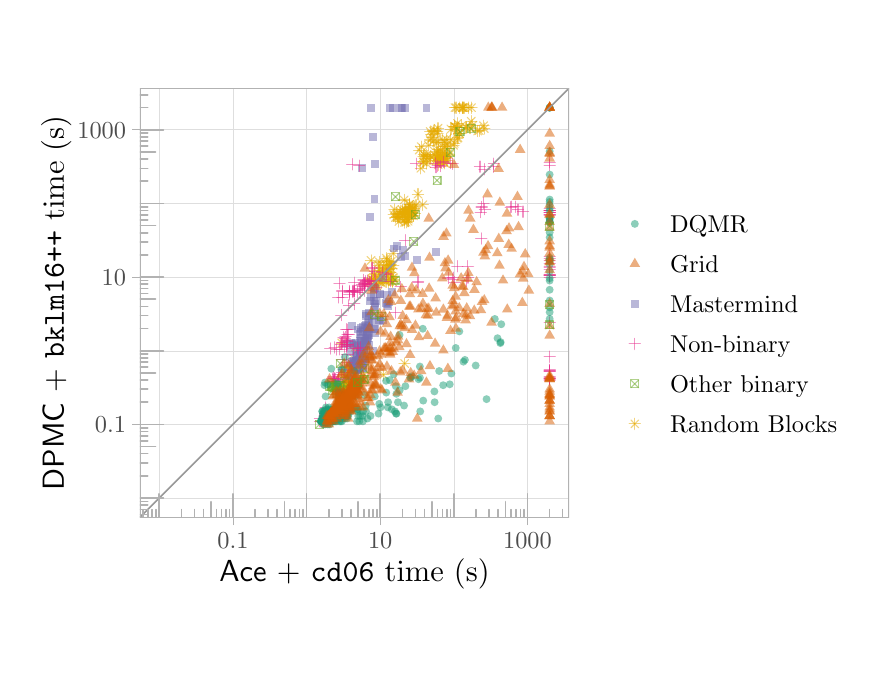
\begin{tikzpicture}[x=1pt,y=1pt]
\definecolor{fillColor}{RGB}{255,255,255}
\path[use as bounding box,fill=fillColor,fill opacity=0.00] (0,0) rectangle (303.53,224.04);
\begin{scope}
\path[clip] (  0.00, 16.35) rectangle (303.53,207.69);
\definecolor{drawColor}{RGB}{255,255,255}
\definecolor{fillColor}{RGB}{255,255,255}

\path[draw=drawColor,line width= 0.6pt,line join=round,line cap=round,fill=fillColor] (  0.00, 16.35) rectangle (303.53,207.69);
\end{scope}
\begin{scope}
\path[clip] ( 40.51, 47.03) rectangle (195.67,202.19);
\definecolor{fillColor}{RGB}{255,255,255}

\path[fill=fillColor] ( 40.51, 47.03) rectangle (195.67,202.19);
\definecolor{drawColor}{gray}{0.87}

\path[draw=drawColor,line width= 0.1pt,line join=round] ( 40.51, 54.09) --
	(195.67, 54.09);

\path[draw=drawColor,line width= 0.1pt,line join=round] ( 40.51,107.30) --
	(195.67,107.30);

\path[draw=drawColor,line width= 0.1pt,line join=round] ( 40.51,160.52) --
	(195.67,160.52);

\path[draw=drawColor,line width= 0.1pt,line join=round] ( 47.56, 47.03) --
	( 47.56,202.19);

\path[draw=drawColor,line width= 0.1pt,line join=round] (100.78, 47.03) --
	(100.78,202.19);

\path[draw=drawColor,line width= 0.1pt,line join=round] (154.00, 47.03) --
	(154.00,202.19);

\path[draw=drawColor,line width= 0.3pt,line join=round] ( 40.51, 80.69) --
	(195.67, 80.69);

\path[draw=drawColor,line width= 0.3pt,line join=round] ( 40.51,133.91) --
	(195.67,133.91);

\path[draw=drawColor,line width= 0.3pt,line join=round] ( 40.51,187.13) --
	(195.67,187.13);

\path[draw=drawColor,line width= 0.3pt,line join=round] ( 74.17, 47.03) --
	( 74.17,202.19);

\path[draw=drawColor,line width= 0.3pt,line join=round] (127.39, 47.03) --
	(127.39,202.19);

\path[draw=drawColor,line width= 0.3pt,line join=round] (180.61, 47.03) --
	(180.61,202.19);
\definecolor{drawColor}{RGB}{230,171,2}

\path[draw=drawColor,draw opacity=0.50,line width= 0.4pt,line join=round,line cap=round] (114.28, 91.57) -- (117.14, 94.42);

\path[draw=drawColor,draw opacity=0.50,line width= 0.4pt,line join=round,line cap=round] (114.28, 94.42) -- (117.14, 91.57);

\path[draw=drawColor,draw opacity=0.50,line width= 0.4pt,line join=round,line cap=round] (113.69, 93.00) -- (117.73, 93.00);

\path[draw=drawColor,draw opacity=0.50,line width= 0.4pt,line join=round,line cap=round] (115.71, 90.98) -- (115.71, 95.01);

\path[draw=drawColor,draw opacity=0.50,line width= 0.4pt,line join=round,line cap=round] (115.63, 91.57) -- (118.48, 94.42);

\path[draw=drawColor,draw opacity=0.50,line width= 0.4pt,line join=round,line cap=round] (115.63, 94.42) -- (118.48, 91.57);

\path[draw=drawColor,draw opacity=0.50,line width= 0.4pt,line join=round,line cap=round] (115.04, 93.00) -- (119.07, 93.00);

\path[draw=drawColor,draw opacity=0.50,line width= 0.4pt,line join=round,line cap=round] (117.06, 90.98) -- (117.06, 95.01);

\path[draw=drawColor,draw opacity=0.50,line width= 0.4pt,line join=round,line cap=round] (113.83, 93.41) -- (116.68, 96.26);

\path[draw=drawColor,draw opacity=0.50,line width= 0.4pt,line join=round,line cap=round] (113.83, 96.26) -- (116.68, 93.41);

\path[draw=drawColor,draw opacity=0.50,line width= 0.4pt,line join=round,line cap=round] (113.24, 94.84) -- (117.27, 94.84);

\path[draw=drawColor,draw opacity=0.50,line width= 0.4pt,line join=round,line cap=round] (115.26, 92.82) -- (115.26, 96.85);

\path[draw=drawColor,draw opacity=0.50,line width= 0.4pt,line join=round,line cap=round] (116.63, 94.07) -- (119.48, 96.92);

\path[draw=drawColor,draw opacity=0.50,line width= 0.4pt,line join=round,line cap=round] (116.63, 96.92) -- (119.48, 94.07);

\path[draw=drawColor,draw opacity=0.50,line width= 0.4pt,line join=round,line cap=round] (116.04, 95.50) -- (120.08, 95.50);

\path[draw=drawColor,draw opacity=0.50,line width= 0.4pt,line join=round,line cap=round] (118.06, 93.48) -- (118.06, 97.51);

\path[draw=drawColor,draw opacity=0.50,line width= 0.4pt,line join=round,line cap=round] (115.77, 93.06) -- (118.62, 95.92);

\path[draw=drawColor,draw opacity=0.50,line width= 0.4pt,line join=round,line cap=round] (115.77, 95.92) -- (118.62, 93.06);

\path[draw=drawColor,draw opacity=0.50,line width= 0.4pt,line join=round,line cap=round] (115.18, 94.49) -- (119.21, 94.49);

\path[draw=drawColor,draw opacity=0.50,line width= 0.4pt,line join=round,line cap=round] (117.20, 92.47) -- (117.20, 96.51);

\path[draw=drawColor,draw opacity=0.50,line width= 0.4pt,line join=round,line cap=round] (114.41, 91.57) -- (117.26, 94.42);

\path[draw=drawColor,draw opacity=0.50,line width= 0.4pt,line join=round,line cap=round] (114.41, 94.42) -- (117.26, 91.57);

\path[draw=drawColor,draw opacity=0.50,line width= 0.4pt,line join=round,line cap=round] (113.82, 93.00) -- (117.85, 93.00);

\path[draw=drawColor,draw opacity=0.50,line width= 0.4pt,line join=round,line cap=round] (115.84, 90.98) -- (115.84, 95.01);

\path[draw=drawColor,draw opacity=0.50,line width= 0.4pt,line join=round,line cap=round] (110.48, 91.96) -- (113.34, 94.82);

\path[draw=drawColor,draw opacity=0.50,line width= 0.4pt,line join=round,line cap=round] (110.48, 94.82) -- (113.34, 91.96);

\path[draw=drawColor,draw opacity=0.50,line width= 0.4pt,line join=round,line cap=round] (109.89, 93.39) -- (113.93, 93.39);

\path[draw=drawColor,draw opacity=0.50,line width= 0.4pt,line join=round,line cap=round] (111.91, 91.37) -- (111.91, 95.41);

\path[draw=drawColor,draw opacity=0.50,line width= 0.4pt,line join=round,line cap=round] (114.90, 93.74) -- (117.75, 96.60);

\path[draw=drawColor,draw opacity=0.50,line width= 0.4pt,line join=round,line cap=round] (114.90, 96.60) -- (117.75, 93.74);

\path[draw=drawColor,draw opacity=0.50,line width= 0.4pt,line join=round,line cap=round] (114.31, 95.17) -- (118.35, 95.17);

\path[draw=drawColor,draw opacity=0.50,line width= 0.4pt,line join=round,line cap=round] (116.33, 93.15) -- (116.33, 97.19);

\path[draw=drawColor,draw opacity=0.50,line width= 0.4pt,line join=round,line cap=round] (113.86, 94.69) -- (116.72, 97.55);

\path[draw=drawColor,draw opacity=0.50,line width= 0.4pt,line join=round,line cap=round] (113.86, 97.55) -- (116.72, 94.69);

\path[draw=drawColor,draw opacity=0.50,line width= 0.4pt,line join=round,line cap=round] (113.27, 96.12) -- (117.31, 96.12);

\path[draw=drawColor,draw opacity=0.50,line width= 0.4pt,line join=round,line cap=round] (115.29, 94.10) -- (115.29, 98.14);

\path[draw=drawColor,draw opacity=0.50,line width= 0.4pt,line join=round,line cap=round] (112.83, 91.17) -- (115.68, 94.02);

\path[draw=drawColor,draw opacity=0.50,line width= 0.4pt,line join=round,line cap=round] (112.83, 94.02) -- (115.68, 91.17);

\path[draw=drawColor,draw opacity=0.50,line width= 0.4pt,line join=round,line cap=round] (112.24, 92.59) -- (116.27, 92.59);

\path[draw=drawColor,draw opacity=0.50,line width= 0.4pt,line join=round,line cap=round] (114.26, 90.57) -- (114.26, 94.61);

\path[draw=drawColor,draw opacity=0.50,line width= 0.4pt,line join=round,line cap=round] (111.33, 92.34) -- (114.19, 95.19);

\path[draw=drawColor,draw opacity=0.50,line width= 0.4pt,line join=round,line cap=round] (111.33, 95.19) -- (114.19, 92.34);

\path[draw=drawColor,draw opacity=0.50,line width= 0.4pt,line join=round,line cap=round] (110.74, 93.77) -- (114.78, 93.77);

\path[draw=drawColor,draw opacity=0.50,line width= 0.4pt,line join=round,line cap=round] (112.76, 91.75) -- (112.76, 95.79);

\path[draw=drawColor,draw opacity=0.50,line width= 0.4pt,line join=round,line cap=round] (115.88, 91.96) -- (118.73, 94.82);

\path[draw=drawColor,draw opacity=0.50,line width= 0.4pt,line join=round,line cap=round] (115.88, 94.82) -- (118.73, 91.96);

\path[draw=drawColor,draw opacity=0.50,line width= 0.4pt,line join=round,line cap=round] (115.29, 93.39) -- (119.33, 93.39);

\path[draw=drawColor,draw opacity=0.50,line width= 0.4pt,line join=round,line cap=round] (117.31, 91.37) -- (117.31, 95.41);

\path[draw=drawColor,draw opacity=0.50,line width= 0.4pt,line join=round,line cap=round] (114.28, 92.71) -- (117.14, 95.56);

\path[draw=drawColor,draw opacity=0.50,line width= 0.4pt,line join=round,line cap=round] (114.28, 95.56) -- (117.14, 92.71);

\path[draw=drawColor,draw opacity=0.50,line width= 0.4pt,line join=round,line cap=round] (113.69, 94.13) -- (117.73, 94.13);

\path[draw=drawColor,draw opacity=0.50,line width= 0.4pt,line join=round,line cap=round] (115.71, 92.12) -- (115.71, 96.15);

\path[draw=drawColor,draw opacity=0.50,line width= 0.4pt,line join=round,line cap=round] (113.46, 91.96) -- (116.31, 94.82);

\path[draw=drawColor,draw opacity=0.50,line width= 0.4pt,line join=round,line cap=round] (113.46, 94.82) -- (116.31, 91.96);

\path[draw=drawColor,draw opacity=0.50,line width= 0.4pt,line join=round,line cap=round] (112.87, 93.39) -- (116.91, 93.39);

\path[draw=drawColor,draw opacity=0.50,line width= 0.4pt,line join=round,line cap=round] (114.89, 91.37) -- (114.89, 95.41);

\path[draw=drawColor,draw opacity=0.50,line width= 0.4pt,line join=round,line cap=round] (116.32, 93.74) -- (119.17, 96.60);

\path[draw=drawColor,draw opacity=0.50,line width= 0.4pt,line join=round,line cap=round] (116.32, 96.60) -- (119.17, 93.74);

\path[draw=drawColor,draw opacity=0.50,line width= 0.4pt,line join=round,line cap=round] (115.72, 95.17) -- (119.76, 95.17);

\path[draw=drawColor,draw opacity=0.50,line width= 0.4pt,line join=round,line cap=round] (117.74, 93.15) -- (117.74, 97.19);

\path[draw=drawColor,draw opacity=0.50,line width= 0.4pt,line join=round,line cap=round] (116.34, 92.71) -- (119.20, 95.56);

\path[draw=drawColor,draw opacity=0.50,line width= 0.4pt,line join=round,line cap=round] (116.34, 95.56) -- (119.20, 92.71);

\path[draw=drawColor,draw opacity=0.50,line width= 0.4pt,line join=round,line cap=round] (115.75, 94.13) -- (119.79, 94.13);

\path[draw=drawColor,draw opacity=0.50,line width= 0.4pt,line join=round,line cap=round] (117.77, 92.12) -- (117.77, 96.15);

\path[draw=drawColor,draw opacity=0.50,line width= 0.4pt,line join=round,line cap=round] (116.21, 97.15) -- (119.06,100.00);

\path[draw=drawColor,draw opacity=0.50,line width= 0.4pt,line join=round,line cap=round] (116.21,100.00) -- (119.06, 97.15);

\path[draw=drawColor,draw opacity=0.50,line width= 0.4pt,line join=round,line cap=round] (115.62, 98.58) -- (119.65, 98.58);

\path[draw=drawColor,draw opacity=0.50,line width= 0.4pt,line join=round,line cap=round] (117.64, 96.56) -- (117.64,100.59);

\path[draw=drawColor,draw opacity=0.50,line width= 0.4pt,line join=round,line cap=round] (116.86, 95.57) -- (119.72, 98.43);

\path[draw=drawColor,draw opacity=0.50,line width= 0.4pt,line join=round,line cap=round] (116.86, 98.43) -- (119.72, 95.57);

\path[draw=drawColor,draw opacity=0.50,line width= 0.4pt,line join=round,line cap=round] (116.27, 97.00) -- (120.31, 97.00);

\path[draw=drawColor,draw opacity=0.50,line width= 0.4pt,line join=round,line cap=round] (118.29, 94.98) -- (118.29, 99.02);

\path[draw=drawColor,draw opacity=0.50,line width= 0.4pt,line join=round,line cap=round] (113.70, 94.39) -- (116.55, 97.24);

\path[draw=drawColor,draw opacity=0.50,line width= 0.4pt,line join=round,line cap=round] (113.70, 97.24) -- (116.55, 94.39);

\path[draw=drawColor,draw opacity=0.50,line width= 0.4pt,line join=round,line cap=round] (113.11, 95.81) -- (117.14, 95.81);

\path[draw=drawColor,draw opacity=0.50,line width= 0.4pt,line join=round,line cap=round] (115.12, 93.80) -- (115.12, 97.83);

\path[draw=drawColor,draw opacity=0.50,line width= 0.4pt,line join=round,line cap=round] (117.50, 94.99) -- (120.36, 97.85);

\path[draw=drawColor,draw opacity=0.50,line width= 0.4pt,line join=round,line cap=round] (117.50, 97.85) -- (120.36, 94.99);

\path[draw=drawColor,draw opacity=0.50,line width= 0.4pt,line join=round,line cap=round] (116.91, 96.42) -- (120.95, 96.42);

\path[draw=drawColor,draw opacity=0.50,line width= 0.4pt,line join=round,line cap=round] (118.93, 94.40) -- (118.93, 98.44);

\path[draw=drawColor,draw opacity=0.50,line width= 0.4pt,line join=round,line cap=round] (114.28, 96.65) -- (117.14, 99.50);

\path[draw=drawColor,draw opacity=0.50,line width= 0.4pt,line join=round,line cap=round] (114.28, 99.50) -- (117.14, 96.65);

\path[draw=drawColor,draw opacity=0.50,line width= 0.4pt,line join=round,line cap=round] (113.69, 98.07) -- (117.73, 98.07);

\path[draw=drawColor,draw opacity=0.50,line width= 0.4pt,line join=round,line cap=round] (115.71, 96.06) -- (115.71,100.09);

\path[draw=drawColor,draw opacity=0.50,line width= 0.4pt,line join=round,line cap=round] (114.28, 93.74) -- (117.14, 96.60);

\path[draw=drawColor,draw opacity=0.50,line width= 0.4pt,line join=round,line cap=round] (114.28, 96.60) -- (117.14, 93.74);

\path[draw=drawColor,draw opacity=0.50,line width= 0.4pt,line join=round,line cap=round] (113.69, 95.17) -- (117.73, 95.17);

\path[draw=drawColor,draw opacity=0.50,line width= 0.4pt,line join=round,line cap=round] (115.71, 93.15) -- (115.71, 97.19);

\path[draw=drawColor,draw opacity=0.50,line width= 0.4pt,line join=round,line cap=round] (112.09,108.64) -- (114.94,111.49);

\path[draw=drawColor,draw opacity=0.50,line width= 0.4pt,line join=round,line cap=round] (112.09,111.49) -- (114.94,108.64);

\path[draw=drawColor,draw opacity=0.50,line width= 0.4pt,line join=round,line cap=round] (111.50,110.06) -- (115.53,110.06);

\path[draw=drawColor,draw opacity=0.50,line width= 0.4pt,line join=round,line cap=round] (113.51,108.05) -- (113.51,112.08);

\path[draw=drawColor,draw opacity=0.50,line width= 0.4pt,line join=round,line cap=round] (113.76, 93.74) -- (116.62, 96.60);

\path[draw=drawColor,draw opacity=0.50,line width= 0.4pt,line join=round,line cap=round] (113.76, 96.60) -- (116.62, 93.74);

\path[draw=drawColor,draw opacity=0.50,line width= 0.4pt,line join=round,line cap=round] (113.17, 95.17) -- (117.21, 95.17);

\path[draw=drawColor,draw opacity=0.50,line width= 0.4pt,line join=round,line cap=round] (115.19, 93.15) -- (115.19, 97.19);

\path[draw=drawColor,draw opacity=0.50,line width= 0.4pt,line join=round,line cap=round] (113.29, 93.74) -- (116.14, 96.60);

\path[draw=drawColor,draw opacity=0.50,line width= 0.4pt,line join=round,line cap=round] (113.29, 96.60) -- (116.14, 93.74);

\path[draw=drawColor,draw opacity=0.50,line width= 0.4pt,line join=round,line cap=round] (112.70, 95.17) -- (116.73, 95.17);

\path[draw=drawColor,draw opacity=0.50,line width= 0.4pt,line join=round,line cap=round] (114.72, 93.15) -- (114.72, 97.19);

\path[draw=drawColor,draw opacity=0.50,line width= 0.4pt,line join=round,line cap=round] (116.21, 95.57) -- (119.06, 98.43);

\path[draw=drawColor,draw opacity=0.50,line width= 0.4pt,line join=round,line cap=round] (116.21, 98.43) -- (119.06, 95.57);

\path[draw=drawColor,draw opacity=0.50,line width= 0.4pt,line join=round,line cap=round] (115.62, 97.00) -- (119.65, 97.00);

\path[draw=drawColor,draw opacity=0.50,line width= 0.4pt,line join=round,line cap=round] (117.64, 94.98) -- (117.64, 99.02);

\path[draw=drawColor,draw opacity=0.50,line width= 0.4pt,line join=round,line cap=round] (117.01, 98.09) -- (119.87,100.95);

\path[draw=drawColor,draw opacity=0.50,line width= 0.4pt,line join=round,line cap=round] (117.01,100.95) -- (119.87, 98.09);

\path[draw=drawColor,draw opacity=0.50,line width= 0.4pt,line join=round,line cap=round] (116.42, 99.52) -- (120.46, 99.52);

\path[draw=drawColor,draw opacity=0.50,line width= 0.4pt,line join=round,line cap=round] (118.44, 97.50) -- (118.44,101.54);

\path[draw=drawColor,draw opacity=0.50,line width= 0.4pt,line join=round,line cap=round] (115.69, 94.69) -- (118.54, 97.55);

\path[draw=drawColor,draw opacity=0.50,line width= 0.4pt,line join=round,line cap=round] (115.69, 97.55) -- (118.54, 94.69);

\path[draw=drawColor,draw opacity=0.50,line width= 0.4pt,line join=round,line cap=round] (115.10, 96.12) -- (119.13, 96.12);

\path[draw=drawColor,draw opacity=0.50,line width= 0.4pt,line join=round,line cap=round] (117.11, 94.10) -- (117.11, 98.14);

\path[draw=drawColor,draw opacity=0.50,line width= 0.4pt,line join=round,line cap=round] (113.01, 93.06) -- (115.86, 95.92);

\path[draw=drawColor,draw opacity=0.50,line width= 0.4pt,line join=round,line cap=round] (113.01, 95.92) -- (115.86, 93.06);

\path[draw=drawColor,draw opacity=0.50,line width= 0.4pt,line join=round,line cap=round] (112.42, 94.49) -- (116.45, 94.49);

\path[draw=drawColor,draw opacity=0.50,line width= 0.4pt,line join=round,line cap=round] (114.44, 92.47) -- (114.44, 96.51);

\path[draw=drawColor,draw opacity=0.50,line width= 0.4pt,line join=round,line cap=round] (114.31, 95.29) -- (117.17, 98.14);

\path[draw=drawColor,draw opacity=0.50,line width= 0.4pt,line join=round,line cap=round] (114.31, 98.14) -- (117.17, 95.29);

\path[draw=drawColor,draw opacity=0.50,line width= 0.4pt,line join=round,line cap=round] (113.72, 96.71) -- (117.76, 96.71);

\path[draw=drawColor,draw opacity=0.50,line width= 0.4pt,line join=round,line cap=round] (115.74, 94.70) -- (115.74, 98.73);

\path[draw=drawColor,draw opacity=0.50,line width= 0.4pt,line join=round,line cap=round] (112.90, 93.06) -- (115.76, 95.92);

\path[draw=drawColor,draw opacity=0.50,line width= 0.4pt,line join=round,line cap=round] (112.90, 95.92) -- (115.76, 93.06);

\path[draw=drawColor,draw opacity=0.50,line width= 0.4pt,line join=round,line cap=round] (112.31, 94.49) -- (116.35, 94.49);

\path[draw=drawColor,draw opacity=0.50,line width= 0.4pt,line join=round,line cap=round] (114.33, 92.47) -- (114.33, 96.51);

\path[draw=drawColor,draw opacity=0.50,line width= 0.4pt,line join=round,line cap=round] (114.63, 97.39) -- (117.48,100.25);

\path[draw=drawColor,draw opacity=0.50,line width= 0.4pt,line join=round,line cap=round] (114.63,100.25) -- (117.48, 97.39);

\path[draw=drawColor,draw opacity=0.50,line width= 0.4pt,line join=round,line cap=round] (114.04, 98.82) -- (118.07, 98.82);

\path[draw=drawColor,draw opacity=0.50,line width= 0.4pt,line join=round,line cap=round] (116.05, 96.80) -- (116.05,100.84);

\path[draw=drawColor,draw opacity=0.50,line width= 0.4pt,line join=round,line cap=round] (117.86,106.33) -- (120.71,109.18);

\path[draw=drawColor,draw opacity=0.50,line width= 0.4pt,line join=round,line cap=round] (117.86,109.18) -- (120.71,106.33);

\path[draw=drawColor,draw opacity=0.50,line width= 0.4pt,line join=round,line cap=round] (117.27,107.76) -- (121.30,107.76);

\path[draw=drawColor,draw opacity=0.50,line width= 0.4pt,line join=round,line cap=round] (119.29,105.74) -- (119.29,109.77);

\path[draw=drawColor,draw opacity=0.50,line width= 0.4pt,line join=round,line cap=round] (114.06, 97.15) -- (116.91,100.00);

\path[draw=drawColor,draw opacity=0.50,line width= 0.4pt,line join=round,line cap=round] (114.06,100.00) -- (116.91, 97.15);

\path[draw=drawColor,draw opacity=0.50,line width= 0.4pt,line join=round,line cap=round] (113.47, 98.58) -- (117.50, 98.58);

\path[draw=drawColor,draw opacity=0.50,line width= 0.4pt,line join=round,line cap=round] (115.49, 96.56) -- (115.49,100.59);

\path[draw=drawColor,draw opacity=0.50,line width= 0.4pt,line join=round,line cap=round] (113.73, 96.12) -- (116.58, 98.98);

\path[draw=drawColor,draw opacity=0.50,line width= 0.4pt,line join=round,line cap=round] (113.73, 98.98) -- (116.58, 96.12);

\path[draw=drawColor,draw opacity=0.50,line width= 0.4pt,line join=round,line cap=round] (113.14, 97.55) -- (117.17, 97.55);

\path[draw=drawColor,draw opacity=0.50,line width= 0.4pt,line join=round,line cap=round] (115.16, 95.53) -- (115.16, 99.57);

\path[draw=drawColor,draw opacity=0.50,line width= 0.4pt,line join=round,line cap=round] (115.49, 96.90) -- (118.34, 99.76);

\path[draw=drawColor,draw opacity=0.50,line width= 0.4pt,line join=round,line cap=round] (115.49, 99.76) -- (118.34, 96.90);

\path[draw=drawColor,draw opacity=0.50,line width= 0.4pt,line join=round,line cap=round] (114.90, 98.33) -- (118.93, 98.33);

\path[draw=drawColor,draw opacity=0.50,line width= 0.4pt,line join=round,line cap=round] (116.91, 96.31) -- (116.91,100.35);

\path[draw=drawColor,draw opacity=0.50,line width= 0.4pt,line join=round,line cap=round] (117.72, 98.54) -- (120.57,101.39);

\path[draw=drawColor,draw opacity=0.50,line width= 0.4pt,line join=round,line cap=round] (117.72,101.39) -- (120.57, 98.54);

\path[draw=drawColor,draw opacity=0.50,line width= 0.4pt,line join=round,line cap=round] (117.13, 99.97) -- (121.16, 99.97);

\path[draw=drawColor,draw opacity=0.50,line width= 0.4pt,line join=round,line cap=round] (119.14, 97.95) -- (119.14,101.98);

\path[draw=drawColor,draw opacity=0.50,line width= 0.4pt,line join=round,line cap=round] (114.41, 95.29) -- (117.26, 98.14);

\path[draw=drawColor,draw opacity=0.50,line width= 0.4pt,line join=round,line cap=round] (114.41, 98.14) -- (117.26, 95.29);

\path[draw=drawColor,draw opacity=0.50,line width= 0.4pt,line join=round,line cap=round] (113.82, 96.71) -- (117.85, 96.71);

\path[draw=drawColor,draw opacity=0.50,line width= 0.4pt,line join=round,line cap=round] (115.84, 94.70) -- (115.84, 98.73);

\path[draw=drawColor,draw opacity=0.50,line width= 0.4pt,line join=round,line cap=round] (116.42,103.00) -- (119.28,105.86);

\path[draw=drawColor,draw opacity=0.50,line width= 0.4pt,line join=round,line cap=round] (116.42,105.86) -- (119.28,103.00);

\path[draw=drawColor,draw opacity=0.50,line width= 0.4pt,line join=round,line cap=round] (115.83,104.43) -- (119.87,104.43);

\path[draw=drawColor,draw opacity=0.50,line width= 0.4pt,line join=round,line cap=round] (117.85,102.41) -- (117.85,106.45);

\path[draw=drawColor,draw opacity=0.50,line width= 0.4pt,line join=round,line cap=round] (116.13, 99.38) -- (118.98,102.23);

\path[draw=drawColor,draw opacity=0.50,line width= 0.4pt,line join=round,line cap=round] (116.13,102.23) -- (118.98, 99.38);

\path[draw=drawColor,draw opacity=0.50,line width= 0.4pt,line join=round,line cap=round] (115.54,100.81) -- (119.57,100.81);

\path[draw=drawColor,draw opacity=0.50,line width= 0.4pt,line join=round,line cap=round] (117.55, 98.79) -- (117.55,102.82);

\path[draw=drawColor,draw opacity=0.50,line width= 0.4pt,line join=round,line cap=round] (117.36, 97.63) -- (120.21,100.49);

\path[draw=drawColor,draw opacity=0.50,line width= 0.4pt,line join=round,line cap=round] (117.36,100.49) -- (120.21, 97.63);

\path[draw=drawColor,draw opacity=0.50,line width= 0.4pt,line join=round,line cap=round] (116.77, 99.06) -- (120.80, 99.06);

\path[draw=drawColor,draw opacity=0.50,line width= 0.4pt,line join=round,line cap=round] (118.79, 97.04) -- (118.79,101.08);

\path[draw=drawColor,draw opacity=0.50,line width= 0.4pt,line join=round,line cap=round] (116.99,107.19) -- (119.84,110.04);

\path[draw=drawColor,draw opacity=0.50,line width= 0.4pt,line join=round,line cap=round] (116.99,110.04) -- (119.84,107.19);

\path[draw=drawColor,draw opacity=0.50,line width= 0.4pt,line join=round,line cap=round] (116.40,108.61) -- (120.43,108.61);

\path[draw=drawColor,draw opacity=0.50,line width= 0.4pt,line join=round,line cap=round] (118.41,106.59) -- (118.41,110.63);

\path[draw=drawColor,draw opacity=0.50,line width= 0.4pt,line join=round,line cap=round] (127.17, 97.15) -- (130.02,100.00);

\path[draw=drawColor,draw opacity=0.50,line width= 0.4pt,line join=round,line cap=round] (127.17,100.00) -- (130.02, 97.15);

\path[draw=drawColor,draw opacity=0.50,line width= 0.4pt,line join=round,line cap=round] (126.58, 98.58) -- (130.61, 98.58);

\path[draw=drawColor,draw opacity=0.50,line width= 0.4pt,line join=round,line cap=round] (128.59, 96.56) -- (128.59,100.59);

\path[draw=drawColor,draw opacity=0.50,line width= 0.4pt,line join=round,line cap=round] (114.53, 96.12) -- (117.39, 98.98);

\path[draw=drawColor,draw opacity=0.50,line width= 0.4pt,line join=round,line cap=round] (114.53, 98.98) -- (117.39, 96.12);

\path[draw=drawColor,draw opacity=0.50,line width= 0.4pt,line join=round,line cap=round] (113.94, 97.55) -- (117.98, 97.55);

\path[draw=drawColor,draw opacity=0.50,line width= 0.4pt,line join=round,line cap=round] (115.96, 95.53) -- (115.96, 99.57);

\path[draw=drawColor,draw opacity=0.50,line width= 0.4pt,line join=round,line cap=round] (113.25, 95.57) -- (116.11, 98.43);

\path[draw=drawColor,draw opacity=0.50,line width= 0.4pt,line join=round,line cap=round] (113.25, 98.43) -- (116.11, 95.57);

\path[draw=drawColor,draw opacity=0.50,line width= 0.4pt,line join=round,line cap=round] (112.66, 97.00) -- (116.70, 97.00);

\path[draw=drawColor,draw opacity=0.50,line width= 0.4pt,line join=round,line cap=round] (114.68, 94.98) -- (114.68, 99.02);

\path[draw=drawColor,draw opacity=0.50,line width= 0.4pt,line join=round,line cap=round] (119.90, 96.90) -- (122.76, 99.76);

\path[draw=drawColor,draw opacity=0.50,line width= 0.4pt,line join=round,line cap=round] (119.90, 99.76) -- (122.76, 96.90);

\path[draw=drawColor,draw opacity=0.50,line width= 0.4pt,line join=round,line cap=round] (119.31, 98.33) -- (123.35, 98.33);

\path[draw=drawColor,draw opacity=0.50,line width= 0.4pt,line join=round,line cap=round] (121.33, 96.31) -- (121.33,100.35);

\path[draw=drawColor,draw opacity=0.50,line width= 0.4pt,line join=round,line cap=round] (114.53, 96.90) -- (117.39, 99.76);

\path[draw=drawColor,draw opacity=0.50,line width= 0.4pt,line join=round,line cap=round] (114.53, 99.76) -- (117.39, 96.90);

\path[draw=drawColor,draw opacity=0.50,line width= 0.4pt,line join=round,line cap=round] (113.94, 98.33) -- (117.98, 98.33);

\path[draw=drawColor,draw opacity=0.50,line width= 0.4pt,line join=round,line cap=round] (115.96, 96.31) -- (115.96,100.35);

\path[draw=drawColor,draw opacity=0.50,line width= 0.4pt,line join=round,line cap=round] (118.40,100.16) -- (121.26,103.02);

\path[draw=drawColor,draw opacity=0.50,line width= 0.4pt,line join=round,line cap=round] (118.40,103.02) -- (121.26,100.16);

\path[draw=drawColor,draw opacity=0.50,line width= 0.4pt,line join=round,line cap=round] (117.81,101.59) -- (121.85,101.59);

\path[draw=drawColor,draw opacity=0.50,line width= 0.4pt,line join=round,line cap=round] (119.83, 99.57) -- (119.83,103.61);

\path[draw=drawColor,draw opacity=0.50,line width= 0.4pt,line join=round,line cap=round] (128.21,130.78) -- (131.07,133.63);

\path[draw=drawColor,draw opacity=0.50,line width= 0.4pt,line join=round,line cap=round] (128.21,133.63) -- (131.07,130.78);

\path[draw=drawColor,draw opacity=0.50,line width= 0.4pt,line join=round,line cap=round] (127.62,132.21) -- (131.66,132.21);

\path[draw=drawColor,draw opacity=0.50,line width= 0.4pt,line join=round,line cap=round] (129.64,130.19) -- (129.64,134.23);

\path[draw=drawColor,draw opacity=0.50,line width= 0.4pt,line join=round,line cap=round] (126.91,132.43) -- (129.77,135.28);

\path[draw=drawColor,draw opacity=0.50,line width= 0.4pt,line join=round,line cap=round] (126.91,135.28) -- (129.77,132.43);

\path[draw=drawColor,draw opacity=0.50,line width= 0.4pt,line join=round,line cap=round] (126.32,133.85) -- (130.36,133.85);

\path[draw=drawColor,draw opacity=0.50,line width= 0.4pt,line join=round,line cap=round] (128.34,131.84) -- (128.34,135.87);

\path[draw=drawColor,draw opacity=0.50,line width= 0.4pt,line join=round,line cap=round] (122.31,130.82) -- (125.16,133.67);

\path[draw=drawColor,draw opacity=0.50,line width= 0.4pt,line join=round,line cap=round] (122.31,133.67) -- (125.16,130.82);

\path[draw=drawColor,draw opacity=0.50,line width= 0.4pt,line join=round,line cap=round] (121.72,132.25) -- (125.75,132.25);

\path[draw=drawColor,draw opacity=0.50,line width= 0.4pt,line join=round,line cap=round] (123.74,130.23) -- (123.74,134.27);

\path[draw=drawColor,draw opacity=0.50,line width= 0.4pt,line join=round,line cap=round] (126.51,130.29) -- (129.37,133.14);

\path[draw=drawColor,draw opacity=0.50,line width= 0.4pt,line join=round,line cap=round] (126.51,133.14) -- (129.37,130.29);

\path[draw=drawColor,draw opacity=0.50,line width= 0.4pt,line join=round,line cap=round] (125.92,131.72) -- (129.96,131.72);

\path[draw=drawColor,draw opacity=0.50,line width= 0.4pt,line join=round,line cap=round] (127.94,129.70) -- (127.94,133.73);

\path[draw=drawColor,draw opacity=0.50,line width= 0.4pt,line join=round,line cap=round] (130.30,130.89) -- (133.16,133.74);

\path[draw=drawColor,draw opacity=0.50,line width= 0.4pt,line join=round,line cap=round] (130.30,133.74) -- (133.16,130.89);

\path[draw=drawColor,draw opacity=0.50,line width= 0.4pt,line join=round,line cap=round] (129.71,132.31) -- (133.75,132.31);

\path[draw=drawColor,draw opacity=0.50,line width= 0.4pt,line join=round,line cap=round] (131.73,130.30) -- (131.73,134.33);

\path[draw=drawColor,draw opacity=0.50,line width= 0.4pt,line join=round,line cap=round] (130.51,130.85) -- (133.36,133.70);

\path[draw=drawColor,draw opacity=0.50,line width= 0.4pt,line join=round,line cap=round] (130.51,133.70) -- (133.36,130.85);

\path[draw=drawColor,draw opacity=0.50,line width= 0.4pt,line join=round,line cap=round] (129.92,132.27) -- (133.95,132.27);

\path[draw=drawColor,draw opacity=0.50,line width= 0.4pt,line join=round,line cap=round] (131.93,130.26) -- (131.93,134.29);

\path[draw=drawColor,draw opacity=0.50,line width= 0.4pt,line join=round,line cap=round] (123.00,131.79) -- (125.85,134.65);

\path[draw=drawColor,draw opacity=0.50,line width= 0.4pt,line join=round,line cap=round] (123.00,134.65) -- (125.85,131.79);

\path[draw=drawColor,draw opacity=0.50,line width= 0.4pt,line join=round,line cap=round] (122.41,133.22) -- (126.45,133.22);

\path[draw=drawColor,draw opacity=0.50,line width= 0.4pt,line join=round,line cap=round] (124.43,131.20) -- (124.43,135.24);

\path[draw=drawColor,draw opacity=0.50,line width= 0.4pt,line join=round,line cap=round] (124.00,130.87) -- (126.85,133.73);

\path[draw=drawColor,draw opacity=0.50,line width= 0.4pt,line join=round,line cap=round] (124.00,133.73) -- (126.85,130.87);

\path[draw=drawColor,draw opacity=0.50,line width= 0.4pt,line join=round,line cap=round] (123.41,132.30) -- (127.45,132.30);

\path[draw=drawColor,draw opacity=0.50,line width= 0.4pt,line join=round,line cap=round] (125.43,130.28) -- (125.43,134.32);

\path[draw=drawColor,draw opacity=0.50,line width= 0.4pt,line join=round,line cap=round] (123.99,130.87) -- (126.84,133.73);

\path[draw=drawColor,draw opacity=0.50,line width= 0.4pt,line join=round,line cap=round] (123.99,133.73) -- (126.84,130.87);

\path[draw=drawColor,draw opacity=0.50,line width= 0.4pt,line join=round,line cap=round] (123.40,132.30) -- (127.43,132.30);

\path[draw=drawColor,draw opacity=0.50,line width= 0.4pt,line join=round,line cap=round] (125.41,130.28) -- (125.41,134.32);

\path[draw=drawColor,draw opacity=0.50,line width= 0.4pt,line join=round,line cap=round] (123.45,131.27) -- (126.31,134.12);

\path[draw=drawColor,draw opacity=0.50,line width= 0.4pt,line join=round,line cap=round] (123.45,134.12) -- (126.31,131.27);

\path[draw=drawColor,draw opacity=0.50,line width= 0.4pt,line join=round,line cap=round] (122.86,132.69) -- (126.90,132.69);

\path[draw=drawColor,draw opacity=0.50,line width= 0.4pt,line join=round,line cap=round] (124.88,130.68) -- (124.88,134.71);

\path[draw=drawColor,draw opacity=0.50,line width= 0.4pt,line join=round,line cap=round] (121.64,130.19) -- (124.49,133.04);

\path[draw=drawColor,draw opacity=0.50,line width= 0.4pt,line join=round,line cap=round] (121.64,133.04) -- (124.49,130.19);

\path[draw=drawColor,draw opacity=0.50,line width= 0.4pt,line join=round,line cap=round] (121.05,131.62) -- (125.08,131.62);

\path[draw=drawColor,draw opacity=0.50,line width= 0.4pt,line join=round,line cap=round] (123.07,129.60) -- (123.07,133.63);

\path[draw=drawColor,draw opacity=0.50,line width= 0.4pt,line join=round,line cap=round] (128.90,130.70) -- (131.75,133.55);

\path[draw=drawColor,draw opacity=0.50,line width= 0.4pt,line join=round,line cap=round] (128.90,133.55) -- (131.75,130.70);

\path[draw=drawColor,draw opacity=0.50,line width= 0.4pt,line join=round,line cap=round] (128.30,132.13) -- (132.34,132.13);

\path[draw=drawColor,draw opacity=0.50,line width= 0.4pt,line join=round,line cap=round] (130.32,130.11) -- (130.32,134.14);

\path[draw=drawColor,draw opacity=0.50,line width= 0.4pt,line join=round,line cap=round] (130.80,132.26) -- (133.65,135.12);

\path[draw=drawColor,draw opacity=0.50,line width= 0.4pt,line join=round,line cap=round] (130.80,135.12) -- (133.65,132.26);

\path[draw=drawColor,draw opacity=0.50,line width= 0.4pt,line join=round,line cap=round] (130.21,133.69) -- (134.24,133.69);

\path[draw=drawColor,draw opacity=0.50,line width= 0.4pt,line join=round,line cap=round] (132.23,131.67) -- (132.23,135.71);

\path[draw=drawColor,draw opacity=0.50,line width= 0.4pt,line join=round,line cap=round] (128.80,131.73) -- (131.65,134.59);

\path[draw=drawColor,draw opacity=0.50,line width= 0.4pt,line join=round,line cap=round] (128.80,134.59) -- (131.65,131.73);

\path[draw=drawColor,draw opacity=0.50,line width= 0.4pt,line join=round,line cap=round] (128.21,133.16) -- (132.24,133.16);

\path[draw=drawColor,draw opacity=0.50,line width= 0.4pt,line join=round,line cap=round] (130.22,131.14) -- (130.22,135.18);

\path[draw=drawColor,draw opacity=0.50,line width= 0.4pt,line join=round,line cap=round] (125.76,130.59) -- (128.62,133.45);

\path[draw=drawColor,draw opacity=0.50,line width= 0.4pt,line join=round,line cap=round] (125.76,133.45) -- (128.62,130.59);

\path[draw=drawColor,draw opacity=0.50,line width= 0.4pt,line join=round,line cap=round] (125.17,132.02) -- (129.21,132.02);

\path[draw=drawColor,draw opacity=0.50,line width= 0.4pt,line join=round,line cap=round] (127.19,130.00) -- (127.19,134.04);

\path[draw=drawColor,draw opacity=0.50,line width= 0.4pt,line join=round,line cap=round] (127.14,134.41) -- (129.99,137.26);

\path[draw=drawColor,draw opacity=0.50,line width= 0.4pt,line join=round,line cap=round] (127.14,137.26) -- (129.99,134.41);

\path[draw=drawColor,draw opacity=0.50,line width= 0.4pt,line join=round,line cap=round] (126.55,135.83) -- (130.58,135.83);

\path[draw=drawColor,draw opacity=0.50,line width= 0.4pt,line join=round,line cap=round] (128.56,133.82) -- (128.56,137.85);

\path[draw=drawColor,draw opacity=0.50,line width= 0.4pt,line join=round,line cap=round] (128.70,134.43) -- (131.55,137.28);

\path[draw=drawColor,draw opacity=0.50,line width= 0.4pt,line join=round,line cap=round] (128.70,137.28) -- (131.55,134.43);

\path[draw=drawColor,draw opacity=0.50,line width= 0.4pt,line join=round,line cap=round] (128.11,135.85) -- (132.14,135.85);

\path[draw=drawColor,draw opacity=0.50,line width= 0.4pt,line join=round,line cap=round] (130.12,133.84) -- (130.12,137.87);

\path[draw=drawColor,draw opacity=0.50,line width= 0.4pt,line join=round,line cap=round] (122.65,138.50) -- (125.51,141.35);

\path[draw=drawColor,draw opacity=0.50,line width= 0.4pt,line join=round,line cap=round] (122.65,141.35) -- (125.51,138.50);

\path[draw=drawColor,draw opacity=0.50,line width= 0.4pt,line join=round,line cap=round] (122.06,139.93) -- (126.10,139.93);

\path[draw=drawColor,draw opacity=0.50,line width= 0.4pt,line join=round,line cap=round] (124.08,137.91) -- (124.08,141.94);

\path[draw=drawColor,draw opacity=0.50,line width= 0.4pt,line join=round,line cap=round] (125.53,134.94) -- (128.38,137.80);

\path[draw=drawColor,draw opacity=0.50,line width= 0.4pt,line join=round,line cap=round] (125.53,137.80) -- (128.38,134.94);

\path[draw=drawColor,draw opacity=0.50,line width= 0.4pt,line join=round,line cap=round] (124.93,136.37) -- (128.97,136.37);

\path[draw=drawColor,draw opacity=0.50,line width= 0.4pt,line join=round,line cap=round] (126.95,134.35) -- (126.95,138.39);

\path[draw=drawColor,draw opacity=0.50,line width= 0.4pt,line join=round,line cap=round] (126.98,131.68) -- (129.83,134.54);

\path[draw=drawColor,draw opacity=0.50,line width= 0.4pt,line join=round,line cap=round] (126.98,134.54) -- (129.83,131.68);

\path[draw=drawColor,draw opacity=0.50,line width= 0.4pt,line join=round,line cap=round] (126.39,133.11) -- (130.42,133.11);

\path[draw=drawColor,draw opacity=0.50,line width= 0.4pt,line join=round,line cap=round] (128.41,131.09) -- (128.41,135.13);

\path[draw=drawColor,draw opacity=0.50,line width= 0.4pt,line join=round,line cap=round] (130.41,132.22) -- (133.26,135.07);

\path[draw=drawColor,draw opacity=0.50,line width= 0.4pt,line join=round,line cap=round] (130.41,135.07) -- (133.26,132.22);

\path[draw=drawColor,draw opacity=0.50,line width= 0.4pt,line join=round,line cap=round] (129.81,133.64) -- (133.85,133.64);

\path[draw=drawColor,draw opacity=0.50,line width= 0.4pt,line join=round,line cap=round] (131.83,131.62) -- (131.83,135.66);

\path[draw=drawColor,draw opacity=0.50,line width= 0.4pt,line join=round,line cap=round] (125.59,131.96) -- (128.44,134.82);

\path[draw=drawColor,draw opacity=0.50,line width= 0.4pt,line join=round,line cap=round] (125.59,134.82) -- (128.44,131.96);

\path[draw=drawColor,draw opacity=0.50,line width= 0.4pt,line join=round,line cap=round] (124.99,133.39) -- (129.03,133.39);

\path[draw=drawColor,draw opacity=0.50,line width= 0.4pt,line join=round,line cap=round] (127.01,131.37) -- (127.01,135.41);

\path[draw=drawColor,draw opacity=0.50,line width= 0.4pt,line join=round,line cap=round] (125.49,131.65) -- (128.34,134.50);

\path[draw=drawColor,draw opacity=0.50,line width= 0.4pt,line join=round,line cap=round] (125.49,134.50) -- (128.34,131.65);

\path[draw=drawColor,draw opacity=0.50,line width= 0.4pt,line join=round,line cap=round] (124.90,133.07) -- (128.93,133.07);

\path[draw=drawColor,draw opacity=0.50,line width= 0.4pt,line join=round,line cap=round] (126.92,131.05) -- (126.92,135.09);

\path[draw=drawColor,draw opacity=0.50,line width= 0.4pt,line join=round,line cap=round] (125.57,133.56) -- (128.43,136.42);

\path[draw=drawColor,draw opacity=0.50,line width= 0.4pt,line join=round,line cap=round] (125.57,136.42) -- (128.43,133.56);

\path[draw=drawColor,draw opacity=0.50,line width= 0.4pt,line join=round,line cap=round] (124.98,134.99) -- (129.02,134.99);

\path[draw=drawColor,draw opacity=0.50,line width= 0.4pt,line join=round,line cap=round] (127.00,132.97) -- (127.00,137.01);

\path[draw=drawColor,draw opacity=0.50,line width= 0.4pt,line join=round,line cap=round] (126.20,131.63) -- (129.06,134.49);

\path[draw=drawColor,draw opacity=0.50,line width= 0.4pt,line join=round,line cap=round] (126.20,134.49) -- (129.06,131.63);

\path[draw=drawColor,draw opacity=0.50,line width= 0.4pt,line join=round,line cap=round] (125.61,133.06) -- (129.65,133.06);

\path[draw=drawColor,draw opacity=0.50,line width= 0.4pt,line join=round,line cap=round] (127.63,131.04) -- (127.63,135.08);

\path[draw=drawColor,draw opacity=0.50,line width= 0.4pt,line join=round,line cap=round] (122.91,131.57) -- (125.76,134.42);

\path[draw=drawColor,draw opacity=0.50,line width= 0.4pt,line join=round,line cap=round] (122.91,134.42) -- (125.76,131.57);

\path[draw=drawColor,draw opacity=0.50,line width= 0.4pt,line join=round,line cap=round] (122.32,133.00) -- (126.36,133.00);

\path[draw=drawColor,draw opacity=0.50,line width= 0.4pt,line join=round,line cap=round] (124.34,130.98) -- (124.34,135.01);

\path[draw=drawColor,draw opacity=0.50,line width= 0.4pt,line join=round,line cap=round] (124.04,133.65) -- (126.90,136.50);

\path[draw=drawColor,draw opacity=0.50,line width= 0.4pt,line join=round,line cap=round] (124.04,136.50) -- (126.90,133.65);

\path[draw=drawColor,draw opacity=0.50,line width= 0.4pt,line join=round,line cap=round] (123.45,135.07) -- (127.49,135.07);

\path[draw=drawColor,draw opacity=0.50,line width= 0.4pt,line join=round,line cap=round] (125.47,133.06) -- (125.47,137.09);

\path[draw=drawColor,draw opacity=0.50,line width= 0.4pt,line join=round,line cap=round] (130.87,131.44) -- (133.72,134.30);

\path[draw=drawColor,draw opacity=0.50,line width= 0.4pt,line join=round,line cap=round] (130.87,134.30) -- (133.72,131.44);

\path[draw=drawColor,draw opacity=0.50,line width= 0.4pt,line join=round,line cap=round] (130.28,132.87) -- (134.31,132.87);

\path[draw=drawColor,draw opacity=0.50,line width= 0.4pt,line join=round,line cap=round] (132.30,130.85) -- (132.30,134.89);

\path[draw=drawColor,draw opacity=0.50,line width= 0.4pt,line join=round,line cap=round] (126.80,134.90) -- (129.65,137.75);

\path[draw=drawColor,draw opacity=0.50,line width= 0.4pt,line join=round,line cap=round] (126.80,137.75) -- (129.65,134.90);

\path[draw=drawColor,draw opacity=0.50,line width= 0.4pt,line join=round,line cap=round] (126.21,136.32) -- (130.24,136.32);

\path[draw=drawColor,draw opacity=0.50,line width= 0.4pt,line join=round,line cap=round] (128.22,134.30) -- (128.22,138.34);

\path[draw=drawColor,draw opacity=0.50,line width= 0.4pt,line join=round,line cap=round] (126.77,132.60) -- (129.62,135.45);

\path[draw=drawColor,draw opacity=0.50,line width= 0.4pt,line join=round,line cap=round] (126.77,135.45) -- (129.62,132.60);

\path[draw=drawColor,draw opacity=0.50,line width= 0.4pt,line join=round,line cap=round] (126.17,134.03) -- (130.21,134.03);

\path[draw=drawColor,draw opacity=0.50,line width= 0.4pt,line join=round,line cap=round] (128.19,132.01) -- (128.19,136.04);

\path[draw=drawColor,draw opacity=0.50,line width= 0.4pt,line join=round,line cap=round] (129.84,132.71) -- (132.69,135.57);

\path[draw=drawColor,draw opacity=0.50,line width= 0.4pt,line join=round,line cap=round] (129.84,135.57) -- (132.69,132.71);

\path[draw=drawColor,draw opacity=0.50,line width= 0.4pt,line join=round,line cap=round] (129.25,134.14) -- (133.29,134.14);

\path[draw=drawColor,draw opacity=0.50,line width= 0.4pt,line join=round,line cap=round] (131.27,132.12) -- (131.27,136.16);

\path[draw=drawColor,draw opacity=0.50,line width= 0.4pt,line join=round,line cap=round] (129.64,134.10) -- (132.49,136.95);

\path[draw=drawColor,draw opacity=0.50,line width= 0.4pt,line join=round,line cap=round] (129.64,136.95) -- (132.49,134.10);

\path[draw=drawColor,draw opacity=0.50,line width= 0.4pt,line join=round,line cap=round] (129.05,135.53) -- (133.09,135.53);

\path[draw=drawColor,draw opacity=0.50,line width= 0.4pt,line join=round,line cap=round] (131.07,133.51) -- (131.07,137.54);

\path[draw=drawColor,draw opacity=0.50,line width= 0.4pt,line join=round,line cap=round] (128.90,135.14) -- (131.75,137.99);

\path[draw=drawColor,draw opacity=0.50,line width= 0.4pt,line join=round,line cap=round] (128.90,137.99) -- (131.75,135.14);

\path[draw=drawColor,draw opacity=0.50,line width= 0.4pt,line join=round,line cap=round] (128.30,136.56) -- (132.34,136.56);

\path[draw=drawColor,draw opacity=0.50,line width= 0.4pt,line join=round,line cap=round] (130.32,134.55) -- (130.32,138.58);

\path[draw=drawColor,draw opacity=0.50,line width= 0.4pt,line join=round,line cap=round] (128.16,139.31) -- (131.02,142.16);

\path[draw=drawColor,draw opacity=0.50,line width= 0.4pt,line join=round,line cap=round] (128.16,142.16) -- (131.02,139.31);

\path[draw=drawColor,draw opacity=0.50,line width= 0.4pt,line join=round,line cap=round] (127.57,140.74) -- (131.61,140.74);

\path[draw=drawColor,draw opacity=0.50,line width= 0.4pt,line join=round,line cap=round] (129.59,138.72) -- (129.59,142.75);

\path[draw=drawColor,draw opacity=0.50,line width= 0.4pt,line join=round,line cap=round] (130.63,136.71) -- (133.48,139.56);

\path[draw=drawColor,draw opacity=0.50,line width= 0.4pt,line join=round,line cap=round] (130.63,139.56) -- (133.48,136.71);

\path[draw=drawColor,draw opacity=0.50,line width= 0.4pt,line join=round,line cap=round] (130.04,138.13) -- (134.08,138.13);

\path[draw=drawColor,draw opacity=0.50,line width= 0.4pt,line join=round,line cap=round] (132.06,136.11) -- (132.06,140.15);

\path[draw=drawColor,draw opacity=0.50,line width= 0.4pt,line join=round,line cap=round] (130.06,135.54) -- (132.92,138.40);

\path[draw=drawColor,draw opacity=0.50,line width= 0.4pt,line join=round,line cap=round] (130.06,138.40) -- (132.92,135.54);

\path[draw=drawColor,draw opacity=0.50,line width= 0.4pt,line join=round,line cap=round] (129.47,136.97) -- (133.51,136.97);

\path[draw=drawColor,draw opacity=0.50,line width= 0.4pt,line join=round,line cap=round] (131.49,134.95) -- (131.49,138.99);

\path[draw=drawColor,draw opacity=0.50,line width= 0.4pt,line join=round,line cap=round] (129.20,136.83) -- (132.06,139.68);

\path[draw=drawColor,draw opacity=0.50,line width= 0.4pt,line join=round,line cap=round] (129.20,139.68) -- (132.06,136.83);

\path[draw=drawColor,draw opacity=0.50,line width= 0.4pt,line join=round,line cap=round] (128.61,138.25) -- (132.65,138.25);

\path[draw=drawColor,draw opacity=0.50,line width= 0.4pt,line join=round,line cap=round] (130.63,136.23) -- (130.63,140.27);

\path[draw=drawColor,draw opacity=0.50,line width= 0.4pt,line join=round,line cap=round] (128.18,137.00) -- (131.04,139.85);

\path[draw=drawColor,draw opacity=0.50,line width= 0.4pt,line join=round,line cap=round] (128.18,139.85) -- (131.04,137.00);

\path[draw=drawColor,draw opacity=0.50,line width= 0.4pt,line join=round,line cap=round] (127.59,138.43) -- (131.63,138.43);

\path[draw=drawColor,draw opacity=0.50,line width= 0.4pt,line join=round,line cap=round] (129.61,136.41) -- (129.61,140.44);

\path[draw=drawColor,draw opacity=0.50,line width= 0.4pt,line join=round,line cap=round] (129.95,138.11) -- (132.80,140.96);

\path[draw=drawColor,draw opacity=0.50,line width= 0.4pt,line join=round,line cap=round] (129.95,140.96) -- (132.80,138.11);

\path[draw=drawColor,draw opacity=0.50,line width= 0.4pt,line join=round,line cap=round] (129.36,139.54) -- (133.39,139.54);

\path[draw=drawColor,draw opacity=0.50,line width= 0.4pt,line join=round,line cap=round] (131.38,137.52) -- (131.38,141.55);

\path[draw=drawColor,draw opacity=0.50,line width= 0.4pt,line join=round,line cap=round] (125.50,136.69) -- (128.36,139.54);

\path[draw=drawColor,draw opacity=0.50,line width= 0.4pt,line join=round,line cap=round] (125.50,139.54) -- (128.36,136.69);

\path[draw=drawColor,draw opacity=0.50,line width= 0.4pt,line join=round,line cap=round] (124.91,138.12) -- (128.95,138.12);

\path[draw=drawColor,draw opacity=0.50,line width= 0.4pt,line join=round,line cap=round] (126.93,136.10) -- (126.93,140.13);

\path[draw=drawColor,draw opacity=0.50,line width= 0.4pt,line join=round,line cap=round] (125.69,137.93) -- (128.55,140.78);

\path[draw=drawColor,draw opacity=0.50,line width= 0.4pt,line join=round,line cap=round] (125.69,140.78) -- (128.55,137.93);

\path[draw=drawColor,draw opacity=0.50,line width= 0.4pt,line join=round,line cap=round] (125.10,139.36) -- (129.14,139.36);

\path[draw=drawColor,draw opacity=0.50,line width= 0.4pt,line join=round,line cap=round] (127.12,137.34) -- (127.12,141.37);

\path[draw=drawColor,draw opacity=0.50,line width= 0.4pt,line join=round,line cap=round] (127.19,135.75) -- (130.04,138.61);

\path[draw=drawColor,draw opacity=0.50,line width= 0.4pt,line join=round,line cap=round] (127.19,138.61) -- (130.04,135.75);

\path[draw=drawColor,draw opacity=0.50,line width= 0.4pt,line join=round,line cap=round] (126.60,137.18) -- (130.63,137.18);

\path[draw=drawColor,draw opacity=0.50,line width= 0.4pt,line join=round,line cap=round] (128.61,135.16) -- (128.61,139.20);

\path[draw=drawColor,draw opacity=0.50,line width= 0.4pt,line join=round,line cap=round] (123.64,133.34) -- (126.49,136.19);

\path[draw=drawColor,draw opacity=0.50,line width= 0.4pt,line join=round,line cap=round] (123.64,136.19) -- (126.49,133.34);

\path[draw=drawColor,draw opacity=0.50,line width= 0.4pt,line join=round,line cap=round] (123.05,134.77) -- (127.08,134.77);

\path[draw=drawColor,draw opacity=0.50,line width= 0.4pt,line join=round,line cap=round] (125.07,132.75) -- (125.07,136.79);

\path[draw=drawColor,draw opacity=0.50,line width= 0.4pt,line join=round,line cap=round] (129.79,136.97) -- (132.65,139.82);

\path[draw=drawColor,draw opacity=0.50,line width= 0.4pt,line join=round,line cap=round] (129.79,139.82) -- (132.65,136.97);

\path[draw=drawColor,draw opacity=0.50,line width= 0.4pt,line join=round,line cap=round] (129.20,138.39) -- (133.24,138.39);

\path[draw=drawColor,draw opacity=0.50,line width= 0.4pt,line join=round,line cap=round] (131.22,136.38) -- (131.22,140.41);

\path[draw=drawColor,draw opacity=0.50,line width= 0.4pt,line join=round,line cap=round] (129.15,136.87) -- (132.01,139.72);

\path[draw=drawColor,draw opacity=0.50,line width= 0.4pt,line join=round,line cap=round] (129.15,139.72) -- (132.01,136.87);

\path[draw=drawColor,draw opacity=0.50,line width= 0.4pt,line join=round,line cap=round] (128.56,138.29) -- (132.60,138.29);

\path[draw=drawColor,draw opacity=0.50,line width= 0.4pt,line join=round,line cap=round] (130.58,136.27) -- (130.58,140.31);

\path[draw=drawColor,draw opacity=0.50,line width= 0.4pt,line join=round,line cap=round] (129.04,135.08) -- (131.89,137.93);

\path[draw=drawColor,draw opacity=0.50,line width= 0.4pt,line join=round,line cap=round] (129.04,137.93) -- (131.89,135.08);

\path[draw=drawColor,draw opacity=0.50,line width= 0.4pt,line join=round,line cap=round] (128.45,136.51) -- (132.48,136.51);

\path[draw=drawColor,draw opacity=0.50,line width= 0.4pt,line join=round,line cap=round] (130.46,134.49) -- (130.46,138.53);

\path[draw=drawColor,draw opacity=0.50,line width= 0.4pt,line join=round,line cap=round] (128.42,138.62) -- (131.27,141.47);

\path[draw=drawColor,draw opacity=0.50,line width= 0.4pt,line join=round,line cap=round] (128.42,141.47) -- (131.27,138.62);

\path[draw=drawColor,draw opacity=0.50,line width= 0.4pt,line join=round,line cap=round] (127.83,140.04) -- (131.86,140.04);

\path[draw=drawColor,draw opacity=0.50,line width= 0.4pt,line join=round,line cap=round] (129.85,138.02) -- (129.85,142.06);

\path[draw=drawColor,draw opacity=0.50,line width= 0.4pt,line join=round,line cap=round] (130.69,141.02) -- (133.54,143.88);

\path[draw=drawColor,draw opacity=0.50,line width= 0.4pt,line join=round,line cap=round] (130.69,143.88) -- (133.54,141.02);

\path[draw=drawColor,draw opacity=0.50,line width= 0.4pt,line join=round,line cap=round] (130.09,142.45) -- (134.13,142.45);

\path[draw=drawColor,draw opacity=0.50,line width= 0.4pt,line join=round,line cap=round] (132.11,140.43) -- (132.11,144.47);

\path[draw=drawColor,draw opacity=0.50,line width= 0.4pt,line join=round,line cap=round] (134.77,152.24) -- (137.63,155.10);

\path[draw=drawColor,draw opacity=0.50,line width= 0.4pt,line join=round,line cap=round] (134.77,155.10) -- (137.63,152.24);

\path[draw=drawColor,draw opacity=0.50,line width= 0.4pt,line join=round,line cap=round] (134.18,153.67) -- (138.22,153.67);

\path[draw=drawColor,draw opacity=0.50,line width= 0.4pt,line join=round,line cap=round] (136.20,151.65) -- (136.20,155.69);

\path[draw=drawColor,draw opacity=0.50,line width= 0.4pt,line join=round,line cap=round] (134.76,153.17) -- (137.61,156.02);

\path[draw=drawColor,draw opacity=0.50,line width= 0.4pt,line join=round,line cap=round] (134.76,156.02) -- (137.61,153.17);

\path[draw=drawColor,draw opacity=0.50,line width= 0.4pt,line join=round,line cap=round] (134.17,154.60) -- (138.20,154.60);

\path[draw=drawColor,draw opacity=0.50,line width= 0.4pt,line join=round,line cap=round] (136.19,152.58) -- (136.19,156.61);

\path[draw=drawColor,draw opacity=0.50,line width= 0.4pt,line join=round,line cap=round] (136.20,153.43) -- (139.06,156.28);

\path[draw=drawColor,draw opacity=0.50,line width= 0.4pt,line join=round,line cap=round] (136.20,156.28) -- (139.06,153.43);

\path[draw=drawColor,draw opacity=0.50,line width= 0.4pt,line join=round,line cap=round] (135.61,154.85) -- (139.65,154.85);

\path[draw=drawColor,draw opacity=0.50,line width= 0.4pt,line join=round,line cap=round] (137.63,152.83) -- (137.63,156.87);

\path[draw=drawColor,draw opacity=0.50,line width= 0.4pt,line join=round,line cap=round] (136.02,152.69) -- (138.87,155.54);

\path[draw=drawColor,draw opacity=0.50,line width= 0.4pt,line join=round,line cap=round] (136.02,155.54) -- (138.87,152.69);

\path[draw=drawColor,draw opacity=0.50,line width= 0.4pt,line join=round,line cap=round] (135.42,154.12) -- (139.46,154.12);

\path[draw=drawColor,draw opacity=0.50,line width= 0.4pt,line join=round,line cap=round] (137.44,152.10) -- (137.44,156.14);

\path[draw=drawColor,draw opacity=0.50,line width= 0.4pt,line join=round,line cap=round] (134.93,155.89) -- (137.78,158.75);

\path[draw=drawColor,draw opacity=0.50,line width= 0.4pt,line join=round,line cap=round] (134.93,158.75) -- (137.78,155.89);

\path[draw=drawColor,draw opacity=0.50,line width= 0.4pt,line join=round,line cap=round] (134.34,157.32) -- (138.37,157.32);

\path[draw=drawColor,draw opacity=0.50,line width= 0.4pt,line join=round,line cap=round] (136.36,155.30) -- (136.36,159.34);

\path[draw=drawColor,draw opacity=0.50,line width= 0.4pt,line join=round,line cap=round] (135.99,154.48) -- (138.84,157.33);

\path[draw=drawColor,draw opacity=0.50,line width= 0.4pt,line join=round,line cap=round] (135.99,157.33) -- (138.84,154.48);

\path[draw=drawColor,draw opacity=0.50,line width= 0.4pt,line join=round,line cap=round] (135.40,155.91) -- (139.44,155.91);

\path[draw=drawColor,draw opacity=0.50,line width= 0.4pt,line join=round,line cap=round] (137.42,153.89) -- (137.42,157.92);

\path[draw=drawColor,draw opacity=0.50,line width= 0.4pt,line join=round,line cap=round] (132.08,154.01) -- (134.93,156.87);

\path[draw=drawColor,draw opacity=0.50,line width= 0.4pt,line join=round,line cap=round] (132.08,156.87) -- (134.93,154.01);

\path[draw=drawColor,draw opacity=0.50,line width= 0.4pt,line join=round,line cap=round] (131.49,155.44) -- (135.52,155.44);

\path[draw=drawColor,draw opacity=0.50,line width= 0.4pt,line join=round,line cap=round] (133.51,153.42) -- (133.51,157.46);

\path[draw=drawColor,draw opacity=0.50,line width= 0.4pt,line join=round,line cap=round] (130.82,155.04) -- (133.68,157.89);

\path[draw=drawColor,draw opacity=0.50,line width= 0.4pt,line join=round,line cap=round] (130.82,157.89) -- (133.68,155.04);

\path[draw=drawColor,draw opacity=0.50,line width= 0.4pt,line join=round,line cap=round] (130.23,156.47) -- (134.27,156.47);

\path[draw=drawColor,draw opacity=0.50,line width= 0.4pt,line join=round,line cap=round] (132.25,154.45) -- (132.25,158.49);

\path[draw=drawColor,draw opacity=0.50,line width= 0.4pt,line join=round,line cap=round] (132.14,154.48) -- (134.99,157.33);

\path[draw=drawColor,draw opacity=0.50,line width= 0.4pt,line join=round,line cap=round] (132.14,157.33) -- (134.99,154.48);

\path[draw=drawColor,draw opacity=0.50,line width= 0.4pt,line join=round,line cap=round] (131.55,155.91) -- (135.59,155.91);

\path[draw=drawColor,draw opacity=0.50,line width= 0.4pt,line join=round,line cap=round] (133.57,153.89) -- (133.57,157.92);

\path[draw=drawColor,draw opacity=0.50,line width= 0.4pt,line join=round,line cap=round] (134.49,155.12) -- (137.34,157.97);

\path[draw=drawColor,draw opacity=0.50,line width= 0.4pt,line join=round,line cap=round] (134.49,157.97) -- (137.34,155.12);

\path[draw=drawColor,draw opacity=0.50,line width= 0.4pt,line join=round,line cap=round] (133.90,156.55) -- (137.94,156.55);

\path[draw=drawColor,draw opacity=0.50,line width= 0.4pt,line join=round,line cap=round] (135.92,154.53) -- (135.92,158.56);

\path[draw=drawColor,draw opacity=0.50,line width= 0.4pt,line join=round,line cap=round] (134.73,156.09) -- (137.59,158.94);

\path[draw=drawColor,draw opacity=0.50,line width= 0.4pt,line join=round,line cap=round] (134.73,158.94) -- (137.59,156.09);

\path[draw=drawColor,draw opacity=0.50,line width= 0.4pt,line join=round,line cap=round] (134.14,157.51) -- (138.18,157.51);

\path[draw=drawColor,draw opacity=0.50,line width= 0.4pt,line join=round,line cap=round] (136.16,155.49) -- (136.16,159.53);

\path[draw=drawColor,draw opacity=0.50,line width= 0.4pt,line join=round,line cap=round] (137.39,155.61) -- (140.24,158.47);

\path[draw=drawColor,draw opacity=0.50,line width= 0.4pt,line join=round,line cap=round] (137.39,158.47) -- (140.24,155.61);

\path[draw=drawColor,draw opacity=0.50,line width= 0.4pt,line join=round,line cap=round] (136.80,157.04) -- (140.83,157.04);

\path[draw=drawColor,draw opacity=0.50,line width= 0.4pt,line join=round,line cap=round] (138.81,155.02) -- (138.81,159.06);

\path[draw=drawColor,draw opacity=0.50,line width= 0.4pt,line join=round,line cap=round] (135.33,152.31) -- (138.18,155.16);

\path[draw=drawColor,draw opacity=0.50,line width= 0.4pt,line join=round,line cap=round] (135.33,155.16) -- (138.18,152.31);

\path[draw=drawColor,draw opacity=0.50,line width= 0.4pt,line join=round,line cap=round] (134.74,153.73) -- (138.77,153.73);

\path[draw=drawColor,draw opacity=0.50,line width= 0.4pt,line join=round,line cap=round] (136.75,151.72) -- (136.75,155.75);

\path[draw=drawColor,draw opacity=0.50,line width= 0.4pt,line join=round,line cap=round] (137.62,155.76) -- (140.48,158.61);

\path[draw=drawColor,draw opacity=0.50,line width= 0.4pt,line join=round,line cap=round] (137.62,158.61) -- (140.48,155.76);

\path[draw=drawColor,draw opacity=0.50,line width= 0.4pt,line join=round,line cap=round] (137.03,157.18) -- (141.07,157.18);

\path[draw=drawColor,draw opacity=0.50,line width= 0.4pt,line join=round,line cap=round] (139.05,155.17) -- (139.05,159.20);

\path[draw=drawColor,draw opacity=0.50,line width= 0.4pt,line join=round,line cap=round] (132.70,152.55) -- (135.55,155.41);

\path[draw=drawColor,draw opacity=0.50,line width= 0.4pt,line join=round,line cap=round] (132.70,155.41) -- (135.55,152.55);

\path[draw=drawColor,draw opacity=0.50,line width= 0.4pt,line join=round,line cap=round] (132.11,153.98) -- (136.14,153.98);

\path[draw=drawColor,draw opacity=0.50,line width= 0.4pt,line join=round,line cap=round] (134.12,151.96) -- (134.12,156.00);

\path[draw=drawColor,draw opacity=0.50,line width= 0.4pt,line join=round,line cap=round] (136.60,154.41) -- (139.45,157.27);

\path[draw=drawColor,draw opacity=0.50,line width= 0.4pt,line join=round,line cap=round] (136.60,157.27) -- (139.45,154.41);

\path[draw=drawColor,draw opacity=0.50,line width= 0.4pt,line join=round,line cap=round] (136.01,155.84) -- (140.05,155.84);

\path[draw=drawColor,draw opacity=0.50,line width= 0.4pt,line join=round,line cap=round] (138.03,153.82) -- (138.03,157.86);

\path[draw=drawColor,draw opacity=0.50,line width= 0.4pt,line join=round,line cap=round] (135.22,154.02) -- (138.08,156.88);

\path[draw=drawColor,draw opacity=0.50,line width= 0.4pt,line join=round,line cap=round] (135.22,156.88) -- (138.08,154.02);

\path[draw=drawColor,draw opacity=0.50,line width= 0.4pt,line join=round,line cap=round] (134.63,155.45) -- (138.67,155.45);

\path[draw=drawColor,draw opacity=0.50,line width= 0.4pt,line join=round,line cap=round] (136.65,153.43) -- (136.65,157.47);

\path[draw=drawColor,draw opacity=0.50,line width= 0.4pt,line join=round,line cap=round] (137.98,154.63) -- (140.84,157.49);

\path[draw=drawColor,draw opacity=0.50,line width= 0.4pt,line join=round,line cap=round] (137.98,157.49) -- (140.84,154.63);

\path[draw=drawColor,draw opacity=0.50,line width= 0.4pt,line join=round,line cap=round] (137.39,156.06) -- (141.43,156.06);

\path[draw=drawColor,draw opacity=0.50,line width= 0.4pt,line join=round,line cap=round] (139.41,154.04) -- (139.41,158.08);

\path[draw=drawColor,draw opacity=0.50,line width= 0.4pt,line join=round,line cap=round] (138.42,157.93) -- (141.28,160.78);

\path[draw=drawColor,draw opacity=0.50,line width= 0.4pt,line join=round,line cap=round] (138.42,160.78) -- (141.28,157.93);

\path[draw=drawColor,draw opacity=0.50,line width= 0.4pt,line join=round,line cap=round] (137.83,159.35) -- (141.87,159.35);

\path[draw=drawColor,draw opacity=0.50,line width= 0.4pt,line join=round,line cap=round] (139.85,157.34) -- (139.85,161.37);

\path[draw=drawColor,draw opacity=0.50,line width= 0.4pt,line join=round,line cap=round] (137.32,154.86) -- (140.18,157.71);

\path[draw=drawColor,draw opacity=0.50,line width= 0.4pt,line join=round,line cap=round] (137.32,157.71) -- (140.18,154.86);

\path[draw=drawColor,draw opacity=0.50,line width= 0.4pt,line join=round,line cap=round] (136.73,156.29) -- (140.77,156.29);

\path[draw=drawColor,draw opacity=0.50,line width= 0.4pt,line join=round,line cap=round] (138.75,154.27) -- (138.75,158.31);

\path[draw=drawColor,draw opacity=0.50,line width= 0.4pt,line join=round,line cap=round] (135.53,153.97) -- (138.38,156.82);

\path[draw=drawColor,draw opacity=0.50,line width= 0.4pt,line join=round,line cap=round] (135.53,156.82) -- (138.38,153.97);

\path[draw=drawColor,draw opacity=0.50,line width= 0.4pt,line join=round,line cap=round] (134.94,155.40) -- (138.97,155.40);

\path[draw=drawColor,draw opacity=0.50,line width= 0.4pt,line join=round,line cap=round] (136.95,153.38) -- (136.95,157.41);

\path[draw=drawColor,draw opacity=0.50,line width= 0.4pt,line join=round,line cap=round] (137.26,155.60) -- (140.12,158.45);

\path[draw=drawColor,draw opacity=0.50,line width= 0.4pt,line join=round,line cap=round] (137.26,158.45) -- (140.12,155.60);

\path[draw=drawColor,draw opacity=0.50,line width= 0.4pt,line join=round,line cap=round] (136.67,157.03) -- (140.71,157.03);

\path[draw=drawColor,draw opacity=0.50,line width= 0.4pt,line join=round,line cap=round] (138.69,155.01) -- (138.69,159.04);

\path[draw=drawColor,draw opacity=0.50,line width= 0.4pt,line join=round,line cap=round] (132.53,154.33) -- (135.39,157.19);

\path[draw=drawColor,draw opacity=0.50,line width= 0.4pt,line join=round,line cap=round] (132.53,157.19) -- (135.39,154.33);

\path[draw=drawColor,draw opacity=0.50,line width= 0.4pt,line join=round,line cap=round] (131.94,155.76) -- (135.98,155.76);

\path[draw=drawColor,draw opacity=0.50,line width= 0.4pt,line join=round,line cap=round] (133.96,153.74) -- (133.96,157.78);

\path[draw=drawColor,draw opacity=0.50,line width= 0.4pt,line join=round,line cap=round] (134.03,155.00) -- (136.88,157.86);

\path[draw=drawColor,draw opacity=0.50,line width= 0.4pt,line join=round,line cap=round] (134.03,157.86) -- (136.88,155.00);

\path[draw=drawColor,draw opacity=0.50,line width= 0.4pt,line join=round,line cap=round] (133.44,156.43) -- (137.47,156.43);

\path[draw=drawColor,draw opacity=0.50,line width= 0.4pt,line join=round,line cap=round] (135.46,154.41) -- (135.46,158.45);

\path[draw=drawColor,draw opacity=0.50,line width= 0.4pt,line join=round,line cap=round] (131.44,153.98) -- (134.30,156.83);

\path[draw=drawColor,draw opacity=0.50,line width= 0.4pt,line join=round,line cap=round] (131.44,156.83) -- (134.30,153.98);

\path[draw=drawColor,draw opacity=0.50,line width= 0.4pt,line join=round,line cap=round] (130.85,155.41) -- (134.89,155.41);

\path[draw=drawColor,draw opacity=0.50,line width= 0.4pt,line join=round,line cap=round] (132.87,153.39) -- (132.87,157.42);

\path[draw=drawColor,draw opacity=0.50,line width= 0.4pt,line join=round,line cap=round] (133.15,156.26) -- (136.00,159.11);

\path[draw=drawColor,draw opacity=0.50,line width= 0.4pt,line join=round,line cap=round] (133.15,159.11) -- (136.00,156.26);

\path[draw=drawColor,draw opacity=0.50,line width= 0.4pt,line join=round,line cap=round] (132.55,157.69) -- (136.59,157.69);

\path[draw=drawColor,draw opacity=0.50,line width= 0.4pt,line join=round,line cap=round] (134.57,155.67) -- (134.57,159.71);

\path[draw=drawColor,draw opacity=0.50,line width= 0.4pt,line join=round,line cap=round] (133.08,154.01) -- (135.94,156.86);

\path[draw=drawColor,draw opacity=0.50,line width= 0.4pt,line join=round,line cap=round] (133.08,156.86) -- (135.94,154.01);

\path[draw=drawColor,draw opacity=0.50,line width= 0.4pt,line join=round,line cap=round] (132.49,155.44) -- (136.53,155.44);

\path[draw=drawColor,draw opacity=0.50,line width= 0.4pt,line join=round,line cap=round] (134.51,153.42) -- (134.51,157.46);

\path[draw=drawColor,draw opacity=0.50,line width= 0.4pt,line join=round,line cap=round] (135.24,155.99) -- (138.09,158.85);

\path[draw=drawColor,draw opacity=0.50,line width= 0.4pt,line join=round,line cap=round] (135.24,158.85) -- (138.09,155.99);

\path[draw=drawColor,draw opacity=0.50,line width= 0.4pt,line join=round,line cap=round] (134.65,157.42) -- (138.68,157.42);

\path[draw=drawColor,draw opacity=0.50,line width= 0.4pt,line join=round,line cap=round] (136.67,155.40) -- (136.67,159.44);

\path[draw=drawColor,draw opacity=0.50,line width= 0.4pt,line join=round,line cap=round] (136.69,158.81) -- (139.54,161.66);

\path[draw=drawColor,draw opacity=0.50,line width= 0.4pt,line join=round,line cap=round] (136.69,161.66) -- (139.54,158.81);

\path[draw=drawColor,draw opacity=0.50,line width= 0.4pt,line join=round,line cap=round] (136.10,160.24) -- (140.13,160.24);

\path[draw=drawColor,draw opacity=0.50,line width= 0.4pt,line join=round,line cap=round] (138.11,158.22) -- (138.11,162.25);

\path[draw=drawColor,draw opacity=0.50,line width= 0.4pt,line join=round,line cap=round] (136.67,157.81) -- (139.53,160.67);

\path[draw=drawColor,draw opacity=0.50,line width= 0.4pt,line join=round,line cap=round] (136.67,160.67) -- (139.53,157.81);

\path[draw=drawColor,draw opacity=0.50,line width= 0.4pt,line join=round,line cap=round] (136.08,159.24) -- (140.12,159.24);

\path[draw=drawColor,draw opacity=0.50,line width= 0.4pt,line join=round,line cap=round] (138.10,157.22) -- (138.10,161.26);

\path[draw=drawColor,draw opacity=0.50,line width= 0.4pt,line join=round,line cap=round] (135.33,156.22) -- (138.18,159.07);

\path[draw=drawColor,draw opacity=0.50,line width= 0.4pt,line join=round,line cap=round] (135.33,159.07) -- (138.18,156.22);

\path[draw=drawColor,draw opacity=0.50,line width= 0.4pt,line join=round,line cap=round] (134.74,157.64) -- (138.77,157.64);

\path[draw=drawColor,draw opacity=0.50,line width= 0.4pt,line join=round,line cap=round] (136.75,155.63) -- (136.75,159.66);

\path[draw=drawColor,draw opacity=0.50,line width= 0.4pt,line join=round,line cap=round] (136.37,157.22) -- (139.23,160.07);

\path[draw=drawColor,draw opacity=0.50,line width= 0.4pt,line join=round,line cap=round] (136.37,160.07) -- (139.23,157.22);

\path[draw=drawColor,draw opacity=0.50,line width= 0.4pt,line join=round,line cap=round] (135.78,158.64) -- (139.82,158.64);

\path[draw=drawColor,draw opacity=0.50,line width= 0.4pt,line join=round,line cap=round] (137.80,156.63) -- (137.80,160.66);

\path[draw=drawColor,draw opacity=0.50,line width= 0.4pt,line join=round,line cap=round] (135.15,156.73) -- (138.00,159.58);

\path[draw=drawColor,draw opacity=0.50,line width= 0.4pt,line join=round,line cap=round] (135.15,159.58) -- (138.00,156.73);

\path[draw=drawColor,draw opacity=0.50,line width= 0.4pt,line join=round,line cap=round] (134.56,158.16) -- (138.59,158.16);

\path[draw=drawColor,draw opacity=0.50,line width= 0.4pt,line join=round,line cap=round] (136.57,156.14) -- (136.57,160.17);

\path[draw=drawColor,draw opacity=0.50,line width= 0.4pt,line join=round,line cap=round] (136.52,158.71) -- (139.37,161.56);

\path[draw=drawColor,draw opacity=0.50,line width= 0.4pt,line join=round,line cap=round] (136.52,161.56) -- (139.37,158.71);

\path[draw=drawColor,draw opacity=0.50,line width= 0.4pt,line join=round,line cap=round] (135.93,160.13) -- (139.96,160.13);

\path[draw=drawColor,draw opacity=0.50,line width= 0.4pt,line join=round,line cap=round] (137.94,158.12) -- (137.94,162.15);

\path[draw=drawColor,draw opacity=0.50,line width= 0.4pt,line join=round,line cap=round] (136.73,155.82) -- (139.58,158.68);

\path[draw=drawColor,draw opacity=0.50,line width= 0.4pt,line join=round,line cap=round] (136.73,158.68) -- (139.58,155.82);

\path[draw=drawColor,draw opacity=0.50,line width= 0.4pt,line join=round,line cap=round] (136.14,157.25) -- (140.17,157.25);

\path[draw=drawColor,draw opacity=0.50,line width= 0.4pt,line join=round,line cap=round] (138.16,155.23) -- (138.16,159.27);

\path[draw=drawColor,draw opacity=0.50,line width= 0.4pt,line join=round,line cap=round] (137.74,157.37) -- (140.59,160.23);

\path[draw=drawColor,draw opacity=0.50,line width= 0.4pt,line join=round,line cap=round] (137.74,160.23) -- (140.59,157.37);

\path[draw=drawColor,draw opacity=0.50,line width= 0.4pt,line join=round,line cap=round] (137.15,158.80) -- (141.18,158.80);

\path[draw=drawColor,draw opacity=0.50,line width= 0.4pt,line join=round,line cap=round] (139.17,156.78) -- (139.17,160.82);

\path[draw=drawColor,draw opacity=0.50,line width= 0.4pt,line join=round,line cap=round] (135.22,156.78) -- (138.08,159.64);

\path[draw=drawColor,draw opacity=0.50,line width= 0.4pt,line join=round,line cap=round] (135.22,159.64) -- (138.08,156.78);

\path[draw=drawColor,draw opacity=0.50,line width= 0.4pt,line join=round,line cap=round] (134.63,158.21) -- (138.67,158.21);

\path[draw=drawColor,draw opacity=0.50,line width= 0.4pt,line join=round,line cap=round] (136.65,156.19) -- (136.65,160.23);

\path[draw=drawColor,draw opacity=0.50,line width= 0.4pt,line join=round,line cap=round] (139.62,162.47) -- (142.47,165.32);

\path[draw=drawColor,draw opacity=0.50,line width= 0.4pt,line join=round,line cap=round] (139.62,165.32) -- (142.47,162.47);

\path[draw=drawColor,draw opacity=0.50,line width= 0.4pt,line join=round,line cap=round] (139.03,163.90) -- (143.06,163.90);

\path[draw=drawColor,draw opacity=0.50,line width= 0.4pt,line join=round,line cap=round] (141.04,161.88) -- (141.04,165.91);

\path[draw=drawColor,draw opacity=0.50,line width= 0.4pt,line join=round,line cap=round] (137.07,157.62) -- (139.92,160.47);

\path[draw=drawColor,draw opacity=0.50,line width= 0.4pt,line join=round,line cap=round] (137.07,160.47) -- (139.92,157.62);

\path[draw=drawColor,draw opacity=0.50,line width= 0.4pt,line join=round,line cap=round] (136.47,159.04) -- (140.51,159.04);

\path[draw=drawColor,draw opacity=0.50,line width= 0.4pt,line join=round,line cap=round] (138.49,157.03) -- (138.49,161.06);

\path[draw=drawColor,draw opacity=0.50,line width= 0.4pt,line join=round,line cap=round] (131.11,156.93) -- (133.96,159.78);

\path[draw=drawColor,draw opacity=0.50,line width= 0.4pt,line join=round,line cap=round] (131.11,159.78) -- (133.96,156.93);

\path[draw=drawColor,draw opacity=0.50,line width= 0.4pt,line join=round,line cap=round] (130.52,158.35) -- (134.55,158.35);

\path[draw=drawColor,draw opacity=0.50,line width= 0.4pt,line join=round,line cap=round] (132.53,156.34) -- (132.53,160.37);

\path[draw=drawColor,draw opacity=0.50,line width= 0.4pt,line join=round,line cap=round] (131.87,155.33) -- (134.73,158.18);

\path[draw=drawColor,draw opacity=0.50,line width= 0.4pt,line join=round,line cap=round] (131.87,158.18) -- (134.73,155.33);

\path[draw=drawColor,draw opacity=0.50,line width= 0.4pt,line join=round,line cap=round] (131.28,156.76) -- (135.32,156.76);

\path[draw=drawColor,draw opacity=0.50,line width= 0.4pt,line join=round,line cap=round] (133.30,154.74) -- (133.30,158.77);

\path[draw=drawColor,draw opacity=0.50,line width= 0.4pt,line join=round,line cap=round] (132.99,155.50) -- (135.84,158.36);

\path[draw=drawColor,draw opacity=0.50,line width= 0.4pt,line join=round,line cap=round] (132.99,158.36) -- (135.84,155.50);

\path[draw=drawColor,draw opacity=0.50,line width= 0.4pt,line join=round,line cap=round] (132.40,156.93) -- (136.43,156.93);

\path[draw=drawColor,draw opacity=0.50,line width= 0.4pt,line join=round,line cap=round] (134.42,154.91) -- (134.42,158.95);

\path[draw=drawColor,draw opacity=0.50,line width= 0.4pt,line join=round,line cap=round] (133.97,156.76) -- (136.82,159.61);

\path[draw=drawColor,draw opacity=0.50,line width= 0.4pt,line join=round,line cap=round] (133.97,159.61) -- (136.82,156.76);

\path[draw=drawColor,draw opacity=0.50,line width= 0.4pt,line join=round,line cap=round] (133.37,158.18) -- (137.41,158.18);

\path[draw=drawColor,draw opacity=0.50,line width= 0.4pt,line join=round,line cap=round] (135.39,156.16) -- (135.39,160.20);

\path[draw=drawColor,draw opacity=0.50,line width= 0.4pt,line join=round,line cap=round] (138.52,155.54) -- (141.37,158.39);

\path[draw=drawColor,draw opacity=0.50,line width= 0.4pt,line join=round,line cap=round] (138.52,158.39) -- (141.37,155.54);

\path[draw=drawColor,draw opacity=0.50,line width= 0.4pt,line join=round,line cap=round] (137.93,156.96) -- (141.97,156.96);

\path[draw=drawColor,draw opacity=0.50,line width= 0.4pt,line join=round,line cap=round] (139.95,154.95) -- (139.95,158.98);

\path[draw=drawColor,draw opacity=0.50,line width= 0.4pt,line join=round,line cap=round] (138.88,158.45) -- (141.74,161.30);

\path[draw=drawColor,draw opacity=0.50,line width= 0.4pt,line join=round,line cap=round] (138.88,161.30) -- (141.74,158.45);

\path[draw=drawColor,draw opacity=0.50,line width= 0.4pt,line join=round,line cap=round] (138.29,159.88) -- (142.33,159.88);

\path[draw=drawColor,draw opacity=0.50,line width= 0.4pt,line join=round,line cap=round] (140.31,157.86) -- (140.31,161.89);

\path[draw=drawColor,draw opacity=0.50,line width= 0.4pt,line join=round,line cap=round] (141.34,158.61) -- (144.20,161.46);

\path[draw=drawColor,draw opacity=0.50,line width= 0.4pt,line join=round,line cap=round] (141.34,161.46) -- (144.20,158.61);

\path[draw=drawColor,draw opacity=0.50,line width= 0.4pt,line join=round,line cap=round] (140.75,160.03) -- (144.79,160.03);

\path[draw=drawColor,draw opacity=0.50,line width= 0.4pt,line join=round,line cap=round] (142.77,158.02) -- (142.77,162.05);

\path[draw=drawColor,draw opacity=0.50,line width= 0.4pt,line join=round,line cap=round] (134.60,160.33) -- (137.45,163.19);

\path[draw=drawColor,draw opacity=0.50,line width= 0.4pt,line join=round,line cap=round] (134.60,163.19) -- (137.45,160.33);

\path[draw=drawColor,draw opacity=0.50,line width= 0.4pt,line join=round,line cap=round] (134.00,161.76) -- (138.04,161.76);

\path[draw=drawColor,draw opacity=0.50,line width= 0.4pt,line join=round,line cap=round] (136.02,159.74) -- (136.02,163.78);

\path[draw=drawColor,draw opacity=0.50,line width= 0.4pt,line join=round,line cap=round] (137.49,156.49) -- (140.34,159.35);

\path[draw=drawColor,draw opacity=0.50,line width= 0.4pt,line join=round,line cap=round] (137.49,159.35) -- (140.34,156.49);

\path[draw=drawColor,draw opacity=0.50,line width= 0.4pt,line join=round,line cap=round] (136.90,157.92) -- (140.93,157.92);

\path[draw=drawColor,draw opacity=0.50,line width= 0.4pt,line join=round,line cap=round] (138.91,155.90) -- (138.91,159.94);

\path[draw=drawColor,draw opacity=0.50,line width= 0.4pt,line join=round,line cap=round] (148.44,175.49) -- (151.29,178.34);

\path[draw=drawColor,draw opacity=0.50,line width= 0.4pt,line join=round,line cap=round] (148.44,178.34) -- (151.29,175.49);

\path[draw=drawColor,draw opacity=0.50,line width= 0.4pt,line join=round,line cap=round] (147.85,176.92) -- (151.88,176.92);

\path[draw=drawColor,draw opacity=0.50,line width= 0.4pt,line join=round,line cap=round] (149.86,174.90) -- (149.86,178.93);

\path[draw=drawColor,draw opacity=0.50,line width= 0.4pt,line join=round,line cap=round] (147.17,174.87) -- (150.02,177.72);

\path[draw=drawColor,draw opacity=0.50,line width= 0.4pt,line join=round,line cap=round] (147.17,177.72) -- (150.02,174.87);

\path[draw=drawColor,draw opacity=0.50,line width= 0.4pt,line join=round,line cap=round] (146.58,176.29) -- (150.61,176.29);

\path[draw=drawColor,draw opacity=0.50,line width= 0.4pt,line join=round,line cap=round] (148.60,174.28) -- (148.60,178.31);

\path[draw=drawColor,draw opacity=0.50,line width= 0.4pt,line join=round,line cap=round] (148.62,177.44) -- (151.48,180.30);

\path[draw=drawColor,draw opacity=0.50,line width= 0.4pt,line join=round,line cap=round] (148.62,180.30) -- (151.48,177.44);

\path[draw=drawColor,draw opacity=0.50,line width= 0.4pt,line join=round,line cap=round] (148.03,178.87) -- (152.07,178.87);

\path[draw=drawColor,draw opacity=0.50,line width= 0.4pt,line join=round,line cap=round] (150.05,176.85) -- (150.05,180.89);

\path[draw=drawColor,draw opacity=0.50,line width= 0.4pt,line join=round,line cap=round] (146.89,173.07) -- (149.74,175.92);

\path[draw=drawColor,draw opacity=0.50,line width= 0.4pt,line join=round,line cap=round] (146.89,175.92) -- (149.74,173.07);

\path[draw=drawColor,draw opacity=0.50,line width= 0.4pt,line join=round,line cap=round] (146.30,174.50) -- (150.33,174.50);

\path[draw=drawColor,draw opacity=0.50,line width= 0.4pt,line join=round,line cap=round] (148.31,172.48) -- (148.31,176.51);

\path[draw=drawColor,draw opacity=0.50,line width= 0.4pt,line join=round,line cap=round] (147.28,174.53) -- (150.14,177.39);

\path[draw=drawColor,draw opacity=0.50,line width= 0.4pt,line join=round,line cap=round] (147.28,177.39) -- (150.14,174.53);

\path[draw=drawColor,draw opacity=0.50,line width= 0.4pt,line join=round,line cap=round] (146.69,175.96) -- (150.73,175.96);

\path[draw=drawColor,draw opacity=0.50,line width= 0.4pt,line join=round,line cap=round] (148.71,173.94) -- (148.71,177.98);

\path[draw=drawColor,draw opacity=0.50,line width= 0.4pt,line join=round,line cap=round] (147.28,174.38) -- (150.14,177.24);

\path[draw=drawColor,draw opacity=0.50,line width= 0.4pt,line join=round,line cap=round] (147.28,177.24) -- (150.14,174.38);

\path[draw=drawColor,draw opacity=0.50,line width= 0.4pt,line join=round,line cap=round] (146.69,175.81) -- (150.73,175.81);

\path[draw=drawColor,draw opacity=0.50,line width= 0.4pt,line join=round,line cap=round] (148.71,173.79) -- (148.71,177.83);

\path[draw=drawColor,draw opacity=0.50,line width= 0.4pt,line join=round,line cap=round] (141.66,174.07) -- (144.51,176.92);

\path[draw=drawColor,draw opacity=0.50,line width= 0.4pt,line join=round,line cap=round] (141.66,176.92) -- (144.51,174.07);

\path[draw=drawColor,draw opacity=0.50,line width= 0.4pt,line join=round,line cap=round] (141.07,175.49) -- (145.10,175.49);

\path[draw=drawColor,draw opacity=0.50,line width= 0.4pt,line join=round,line cap=round] (143.08,173.48) -- (143.08,177.51);

\path[draw=drawColor,draw opacity=0.50,line width= 0.4pt,line join=round,line cap=round] (146.62,177.73) -- (149.48,180.58);

\path[draw=drawColor,draw opacity=0.50,line width= 0.4pt,line join=round,line cap=round] (146.62,180.58) -- (149.48,177.73);

\path[draw=drawColor,draw opacity=0.50,line width= 0.4pt,line join=round,line cap=round] (146.03,179.15) -- (150.07,179.15);

\path[draw=drawColor,draw opacity=0.50,line width= 0.4pt,line join=round,line cap=round] (148.05,177.14) -- (148.05,181.17);

\path[draw=drawColor,draw opacity=0.50,line width= 0.4pt,line join=round,line cap=round] (143.95,175.18) -- (146.80,178.04);

\path[draw=drawColor,draw opacity=0.50,line width= 0.4pt,line join=round,line cap=round] (143.95,178.04) -- (146.80,175.18);

\path[draw=drawColor,draw opacity=0.50,line width= 0.4pt,line join=round,line cap=round] (143.35,176.61) -- (147.39,176.61);

\path[draw=drawColor,draw opacity=0.50,line width= 0.4pt,line join=round,line cap=round] (145.37,174.59) -- (145.37,178.63);

\path[draw=drawColor,draw opacity=0.50,line width= 0.4pt,line join=round,line cap=round] (140.65,171.83) -- (143.50,174.68);

\path[draw=drawColor,draw opacity=0.50,line width= 0.4pt,line join=round,line cap=round] (140.65,174.68) -- (143.50,171.83);

\path[draw=drawColor,draw opacity=0.50,line width= 0.4pt,line join=round,line cap=round] (140.06,173.25) -- (144.09,173.25);

\path[draw=drawColor,draw opacity=0.50,line width= 0.4pt,line join=round,line cap=round] (142.07,171.24) -- (142.07,175.27);

\path[draw=drawColor,draw opacity=0.50,line width= 0.4pt,line join=round,line cap=round] (141.80,176.79) -- (144.65,179.64);

\path[draw=drawColor,draw opacity=0.50,line width= 0.4pt,line join=round,line cap=round] (141.80,179.64) -- (144.65,176.79);

\path[draw=drawColor,draw opacity=0.50,line width= 0.4pt,line join=round,line cap=round] (141.20,178.22) -- (145.24,178.22);

\path[draw=drawColor,draw opacity=0.50,line width= 0.4pt,line join=round,line cap=round] (143.22,176.20) -- (143.22,180.23);

\path[draw=drawColor,draw opacity=0.50,line width= 0.4pt,line join=round,line cap=round] (145.99,174.49) -- (148.84,177.35);

\path[draw=drawColor,draw opacity=0.50,line width= 0.4pt,line join=round,line cap=round] (145.99,177.35) -- (148.84,174.49);

\path[draw=drawColor,draw opacity=0.50,line width= 0.4pt,line join=round,line cap=round] (145.40,175.92) -- (149.44,175.92);

\path[draw=drawColor,draw opacity=0.50,line width= 0.4pt,line join=round,line cap=round] (147.42,173.90) -- (147.42,177.94);

\path[draw=drawColor,draw opacity=0.50,line width= 0.4pt,line join=round,line cap=round] (150.11,174.48) -- (152.96,177.33);

\path[draw=drawColor,draw opacity=0.50,line width= 0.4pt,line join=round,line cap=round] (150.11,177.33) -- (152.96,174.48);

\path[draw=drawColor,draw opacity=0.50,line width= 0.4pt,line join=round,line cap=round] (149.52,175.90) -- (153.55,175.90);

\path[draw=drawColor,draw opacity=0.50,line width= 0.4pt,line join=round,line cap=round] (151.53,173.89) -- (151.53,177.92);

\path[draw=drawColor,draw opacity=0.50,line width= 0.4pt,line join=round,line cap=round] (149.04,174.03) -- (151.89,176.88);

\path[draw=drawColor,draw opacity=0.50,line width= 0.4pt,line join=round,line cap=round] (149.04,176.88) -- (151.89,174.03);

\path[draw=drawColor,draw opacity=0.50,line width= 0.4pt,line join=round,line cap=round] (148.45,175.45) -- (152.48,175.45);

\path[draw=drawColor,draw opacity=0.50,line width= 0.4pt,line join=round,line cap=round] (150.46,173.44) -- (150.46,177.47);

\path[draw=drawColor,draw opacity=0.50,line width= 0.4pt,line join=round,line cap=round] (149.34,175.55) -- (152.19,178.40);

\path[draw=drawColor,draw opacity=0.50,line width= 0.4pt,line join=round,line cap=round] (149.34,178.40) -- (152.19,175.55);

\path[draw=drawColor,draw opacity=0.50,line width= 0.4pt,line join=round,line cap=round] (148.75,176.98) -- (152.78,176.98);

\path[draw=drawColor,draw opacity=0.50,line width= 0.4pt,line join=round,line cap=round] (150.77,174.96) -- (150.77,178.99);

\path[draw=drawColor,draw opacity=0.50,line width= 0.4pt,line join=round,line cap=round] (145.59,176.75) -- (148.44,179.60);

\path[draw=drawColor,draw opacity=0.50,line width= 0.4pt,line join=round,line cap=round] (145.59,179.60) -- (148.44,176.75);

\path[draw=drawColor,draw opacity=0.50,line width= 0.4pt,line join=round,line cap=round] (145.00,178.17) -- (149.03,178.17);

\path[draw=drawColor,draw opacity=0.50,line width= 0.4pt,line join=round,line cap=round] (147.01,176.16) -- (147.01,180.19);

\path[draw=drawColor,draw opacity=0.50,line width= 0.4pt,line join=round,line cap=round] (150.84,176.62) -- (153.70,179.47);

\path[draw=drawColor,draw opacity=0.50,line width= 0.4pt,line join=round,line cap=round] (150.84,179.47) -- (153.70,176.62);

\path[draw=drawColor,draw opacity=0.50,line width= 0.4pt,line join=round,line cap=round] (150.25,178.04) -- (154.29,178.04);

\path[draw=drawColor,draw opacity=0.50,line width= 0.4pt,line join=round,line cap=round] (152.27,176.03) -- (152.27,180.06);

\path[draw=drawColor,draw opacity=0.50,line width= 0.4pt,line join=round,line cap=round] (149.29,173.64) -- (152.14,176.50);

\path[draw=drawColor,draw opacity=0.50,line width= 0.4pt,line join=round,line cap=round] (149.29,176.50) -- (152.14,173.64);

\path[draw=drawColor,draw opacity=0.50,line width= 0.4pt,line join=round,line cap=round] (148.70,175.07) -- (152.73,175.07);

\path[draw=drawColor,draw opacity=0.50,line width= 0.4pt,line join=round,line cap=round] (150.72,173.05) -- (150.72,177.09);

\path[draw=drawColor,draw opacity=0.50,line width= 0.4pt,line join=round,line cap=round] (147.09,176.52) -- (149.94,179.37);

\path[draw=drawColor,draw opacity=0.50,line width= 0.4pt,line join=round,line cap=round] (147.09,179.37) -- (149.94,176.52);

\path[draw=drawColor,draw opacity=0.50,line width= 0.4pt,line join=round,line cap=round] (146.50,177.94) -- (150.53,177.94);

\path[draw=drawColor,draw opacity=0.50,line width= 0.4pt,line join=round,line cap=round] (148.51,175.93) -- (148.51,179.96);

\path[draw=drawColor,draw opacity=0.50,line width= 0.4pt,line join=round,line cap=round] (149.59,175.51) -- (152.44,178.36);

\path[draw=drawColor,draw opacity=0.50,line width= 0.4pt,line join=round,line cap=round] (149.59,178.36) -- (152.44,175.51);

\path[draw=drawColor,draw opacity=0.50,line width= 0.4pt,line join=round,line cap=round] (148.99,176.94) -- (153.03,176.94);

\path[draw=drawColor,draw opacity=0.50,line width= 0.4pt,line join=round,line cap=round] (151.01,174.92) -- (151.01,178.95);

\path[draw=drawColor,draw opacity=0.50,line width= 0.4pt,line join=round,line cap=round] (150.27,180.37) -- (153.12,183.22);

\path[draw=drawColor,draw opacity=0.50,line width= 0.4pt,line join=round,line cap=round] (150.27,183.22) -- (153.12,180.37);

\path[draw=drawColor,draw opacity=0.50,line width= 0.4pt,line join=round,line cap=round] (149.68,181.80) -- (153.71,181.80);

\path[draw=drawColor,draw opacity=0.50,line width= 0.4pt,line join=round,line cap=round] (151.70,179.78) -- (151.70,183.81);

\path[draw=drawColor,draw opacity=0.50,line width= 0.4pt,line join=round,line cap=round] (149.07,176.54) -- (151.93,179.39);

\path[draw=drawColor,draw opacity=0.50,line width= 0.4pt,line join=round,line cap=round] (149.07,179.39) -- (151.93,176.54);

\path[draw=drawColor,draw opacity=0.50,line width= 0.4pt,line join=round,line cap=round] (148.48,177.96) -- (152.52,177.96);

\path[draw=drawColor,draw opacity=0.50,line width= 0.4pt,line join=round,line cap=round] (150.50,175.95) -- (150.50,179.98);

\path[draw=drawColor,draw opacity=0.50,line width= 0.4pt,line join=round,line cap=round] (146.29,175.70) -- (149.14,178.56);

\path[draw=drawColor,draw opacity=0.50,line width= 0.4pt,line join=round,line cap=round] (146.29,178.56) -- (149.14,175.70);

\path[draw=drawColor,draw opacity=0.50,line width= 0.4pt,line join=round,line cap=round] (145.69,177.13) -- (149.73,177.13);

\path[draw=drawColor,draw opacity=0.50,line width= 0.4pt,line join=round,line cap=round] (147.71,175.11) -- (147.71,179.15);

\path[draw=drawColor,draw opacity=0.50,line width= 0.4pt,line join=round,line cap=round] (141.62,175.95) -- (144.48,178.81);

\path[draw=drawColor,draw opacity=0.50,line width= 0.4pt,line join=round,line cap=round] (141.62,178.81) -- (144.48,175.95);

\path[draw=drawColor,draw opacity=0.50,line width= 0.4pt,line join=round,line cap=round] (141.03,177.38) -- (145.07,177.38);

\path[draw=drawColor,draw opacity=0.50,line width= 0.4pt,line join=round,line cap=round] (143.05,175.36) -- (143.05,179.40);

\path[draw=drawColor,draw opacity=0.50,line width= 0.4pt,line join=round,line cap=round] (142.29,176.22) -- (145.15,179.08);

\path[draw=drawColor,draw opacity=0.50,line width= 0.4pt,line join=round,line cap=round] (142.29,179.08) -- (145.15,176.22);

\path[draw=drawColor,draw opacity=0.50,line width= 0.4pt,line join=round,line cap=round] (141.70,177.65) -- (145.74,177.65);

\path[draw=drawColor,draw opacity=0.50,line width= 0.4pt,line join=round,line cap=round] (143.72,175.63) -- (143.72,179.67);

\path[draw=drawColor,draw opacity=0.50,line width= 0.4pt,line join=round,line cap=round] (142.72,173.55) -- (145.58,176.40);

\path[draw=drawColor,draw opacity=0.50,line width= 0.4pt,line join=round,line cap=round] (142.72,176.40) -- (145.58,173.55);

\path[draw=drawColor,draw opacity=0.50,line width= 0.4pt,line join=round,line cap=round] (142.13,174.98) -- (146.17,174.98);

\path[draw=drawColor,draw opacity=0.50,line width= 0.4pt,line join=round,line cap=round] (144.15,172.96) -- (144.15,176.99);

\path[draw=drawColor,draw opacity=0.50,line width= 0.4pt,line join=round,line cap=round] (142.84,176.58) -- (145.69,179.44);

\path[draw=drawColor,draw opacity=0.50,line width= 0.4pt,line join=round,line cap=round] (142.84,179.44) -- (145.69,176.58);

\path[draw=drawColor,draw opacity=0.50,line width= 0.4pt,line join=round,line cap=round] (142.25,178.01) -- (146.28,178.01);

\path[draw=drawColor,draw opacity=0.50,line width= 0.4pt,line join=round,line cap=round] (144.26,175.99) -- (144.26,180.03);

\path[draw=drawColor,draw opacity=0.50,line width= 0.4pt,line join=round,line cap=round] (147.88,174.91) -- (150.73,177.77);

\path[draw=drawColor,draw opacity=0.50,line width= 0.4pt,line join=round,line cap=round] (147.88,177.77) -- (150.73,174.91);

\path[draw=drawColor,draw opacity=0.50,line width= 0.4pt,line join=round,line cap=round] (147.29,176.34) -- (151.32,176.34);

\path[draw=drawColor,draw opacity=0.50,line width= 0.4pt,line join=round,line cap=round] (149.31,174.32) -- (149.31,178.36);

\path[draw=drawColor,draw opacity=0.50,line width= 0.4pt,line join=round,line cap=round] (149.05,175.45) -- (151.90,178.31);

\path[draw=drawColor,draw opacity=0.50,line width= 0.4pt,line join=round,line cap=round] (149.05,178.31) -- (151.90,175.45);

\path[draw=drawColor,draw opacity=0.50,line width= 0.4pt,line join=round,line cap=round] (148.46,176.88) -- (152.49,176.88);

\path[draw=drawColor,draw opacity=0.50,line width= 0.4pt,line join=round,line cap=round] (150.47,174.86) -- (150.47,178.90);

\path[draw=drawColor,draw opacity=0.50,line width= 0.4pt,line join=round,line cap=round] (147.92,174.52) -- (150.78,177.37);

\path[draw=drawColor,draw opacity=0.50,line width= 0.4pt,line join=round,line cap=round] (147.92,177.37) -- (150.78,174.52);

\path[draw=drawColor,draw opacity=0.50,line width= 0.4pt,line join=round,line cap=round] (147.33,175.95) -- (151.37,175.95);

\path[draw=drawColor,draw opacity=0.50,line width= 0.4pt,line join=round,line cap=round] (149.35,173.93) -- (149.35,177.96);

\path[draw=drawColor,draw opacity=0.50,line width= 0.4pt,line join=round,line cap=round] (146.47,175.78) -- (149.33,178.63);

\path[draw=drawColor,draw opacity=0.50,line width= 0.4pt,line join=round,line cap=round] (146.47,178.63) -- (149.33,175.78);

\path[draw=drawColor,draw opacity=0.50,line width= 0.4pt,line join=round,line cap=round] (145.88,177.20) -- (149.92,177.20);

\path[draw=drawColor,draw opacity=0.50,line width= 0.4pt,line join=round,line cap=round] (147.90,175.19) -- (147.90,179.22);

\path[draw=drawColor,draw opacity=0.50,line width= 0.4pt,line join=round,line cap=round] (146.46,177.35) -- (149.32,180.21);

\path[draw=drawColor,draw opacity=0.50,line width= 0.4pt,line join=round,line cap=round] (146.46,180.21) -- (149.32,177.35);

\path[draw=drawColor,draw opacity=0.50,line width= 0.4pt,line join=round,line cap=round] (145.87,178.78) -- (149.91,178.78);

\path[draw=drawColor,draw opacity=0.50,line width= 0.4pt,line join=round,line cap=round] (147.89,176.76) -- (147.89,180.80);

\path[draw=drawColor,draw opacity=0.50,line width= 0.4pt,line join=round,line cap=round] (149.58,179.65) -- (152.43,182.50);

\path[draw=drawColor,draw opacity=0.50,line width= 0.4pt,line join=round,line cap=round] (149.58,182.50) -- (152.43,179.65);

\path[draw=drawColor,draw opacity=0.50,line width= 0.4pt,line join=round,line cap=round] (148.99,181.07) -- (153.02,181.07);

\path[draw=drawColor,draw opacity=0.50,line width= 0.4pt,line join=round,line cap=round] (151.00,179.06) -- (151.00,183.09);

\path[draw=drawColor,draw opacity=0.50,line width= 0.4pt,line join=round,line cap=round] (150.27,178.96) -- (153.13,181.81);

\path[draw=drawColor,draw opacity=0.50,line width= 0.4pt,line join=round,line cap=round] (150.27,181.81) -- (153.13,178.96);

\path[draw=drawColor,draw opacity=0.50,line width= 0.4pt,line join=round,line cap=round] (149.68,180.39) -- (153.72,180.39);

\path[draw=drawColor,draw opacity=0.50,line width= 0.4pt,line join=round,line cap=round] (151.70,178.37) -- (151.70,182.40);

\path[draw=drawColor,draw opacity=0.50,line width= 0.4pt,line join=round,line cap=round] (149.07,179.64) -- (151.92,182.49);

\path[draw=drawColor,draw opacity=0.50,line width= 0.4pt,line join=round,line cap=round] (149.07,182.49) -- (151.92,179.64);

\path[draw=drawColor,draw opacity=0.50,line width= 0.4pt,line join=round,line cap=round] (148.48,181.06) -- (152.51,181.06);

\path[draw=drawColor,draw opacity=0.50,line width= 0.4pt,line join=round,line cap=round] (150.49,179.05) -- (150.49,183.08);

\path[draw=drawColor,draw opacity=0.50,line width= 0.4pt,line join=round,line cap=round] (148.42,176.26) -- (151.27,179.11);

\path[draw=drawColor,draw opacity=0.50,line width= 0.4pt,line join=round,line cap=round] (148.42,179.11) -- (151.27,176.26);

\path[draw=drawColor,draw opacity=0.50,line width= 0.4pt,line join=round,line cap=round] (147.82,177.68) -- (151.86,177.68);

\path[draw=drawColor,draw opacity=0.50,line width= 0.4pt,line join=round,line cap=round] (149.84,175.67) -- (149.84,179.70);

\path[draw=drawColor,draw opacity=0.50,line width= 0.4pt,line join=round,line cap=round] (149.27,181.05) -- (152.13,183.90);

\path[draw=drawColor,draw opacity=0.50,line width= 0.4pt,line join=round,line cap=round] (149.27,183.90) -- (152.13,181.05);

\path[draw=drawColor,draw opacity=0.50,line width= 0.4pt,line join=round,line cap=round] (148.68,182.48) -- (152.72,182.48);

\path[draw=drawColor,draw opacity=0.50,line width= 0.4pt,line join=round,line cap=round] (150.70,180.46) -- (150.70,184.49);

\path[draw=drawColor,draw opacity=0.50,line width= 0.4pt,line join=round,line cap=round] (150.23,177.15) -- (153.09,180.00);

\path[draw=drawColor,draw opacity=0.50,line width= 0.4pt,line join=round,line cap=round] (150.23,180.00) -- (153.09,177.15);

\path[draw=drawColor,draw opacity=0.50,line width= 0.4pt,line join=round,line cap=round] (149.64,178.57) -- (153.68,178.57);

\path[draw=drawColor,draw opacity=0.50,line width= 0.4pt,line join=round,line cap=round] (151.66,176.56) -- (151.66,180.59);

\path[draw=drawColor,draw opacity=0.50,line width= 0.4pt,line join=round,line cap=round] (141.40,174.13) -- (144.26,176.98);

\path[draw=drawColor,draw opacity=0.50,line width= 0.4pt,line join=round,line cap=round] (141.40,176.98) -- (144.26,174.13);

\path[draw=drawColor,draw opacity=0.50,line width= 0.4pt,line join=round,line cap=round] (140.81,175.55) -- (144.85,175.55);

\path[draw=drawColor,draw opacity=0.50,line width= 0.4pt,line join=round,line cap=round] (142.83,173.54) -- (142.83,177.57);

\path[draw=drawColor,draw opacity=0.50,line width= 0.4pt,line join=round,line cap=round] (140.06,178.39) -- (142.91,181.24);

\path[draw=drawColor,draw opacity=0.50,line width= 0.4pt,line join=round,line cap=round] (140.06,181.24) -- (142.91,178.39);

\path[draw=drawColor,draw opacity=0.50,line width= 0.4pt,line join=round,line cap=round] (139.47,179.81) -- (143.50,179.81);

\path[draw=drawColor,draw opacity=0.50,line width= 0.4pt,line join=round,line cap=round] (141.49,177.80) -- (141.49,181.83);

\path[draw=drawColor,draw opacity=0.50,line width= 0.4pt,line join=round,line cap=round] (140.80,179.61) -- (143.65,182.47);

\path[draw=drawColor,draw opacity=0.50,line width= 0.4pt,line join=round,line cap=round] (140.80,182.47) -- (143.65,179.61);

\path[draw=drawColor,draw opacity=0.50,line width= 0.4pt,line join=round,line cap=round] (140.21,181.04) -- (144.24,181.04);

\path[draw=drawColor,draw opacity=0.50,line width= 0.4pt,line join=round,line cap=round] (142.23,179.02) -- (142.23,183.06);

\path[draw=drawColor,draw opacity=0.50,line width= 0.4pt,line join=round,line cap=round] (143.00,175.42) -- (145.85,178.27);

\path[draw=drawColor,draw opacity=0.50,line width= 0.4pt,line join=round,line cap=round] (143.00,178.27) -- (145.85,175.42);

\path[draw=drawColor,draw opacity=0.50,line width= 0.4pt,line join=round,line cap=round] (142.41,176.85) -- (146.45,176.85);

\path[draw=drawColor,draw opacity=0.50,line width= 0.4pt,line join=round,line cap=round] (144.43,174.83) -- (144.43,178.87);

\path[draw=drawColor,draw opacity=0.50,line width= 0.4pt,line join=round,line cap=round] (144.27,176.00) -- (147.12,178.86);

\path[draw=drawColor,draw opacity=0.50,line width= 0.4pt,line join=round,line cap=round] (144.27,178.86) -- (147.12,176.00);

\path[draw=drawColor,draw opacity=0.50,line width= 0.4pt,line join=round,line cap=round] (143.68,177.43) -- (147.71,177.43);

\path[draw=drawColor,draw opacity=0.50,line width= 0.4pt,line join=round,line cap=round] (145.69,175.41) -- (145.69,179.45);

\path[draw=drawColor,draw opacity=0.50,line width= 0.4pt,line join=round,line cap=round] (148.54,176.14) -- (151.39,178.99);

\path[draw=drawColor,draw opacity=0.50,line width= 0.4pt,line join=round,line cap=round] (148.54,178.99) -- (151.39,176.14);

\path[draw=drawColor,draw opacity=0.50,line width= 0.4pt,line join=round,line cap=round] (147.95,177.57) -- (151.98,177.57);

\path[draw=drawColor,draw opacity=0.50,line width= 0.4pt,line join=round,line cap=round] (149.97,175.55) -- (149.97,179.59);

\path[draw=drawColor,draw opacity=0.50,line width= 0.4pt,line join=round,line cap=round] (148.72,176.19) -- (151.57,179.04);

\path[draw=drawColor,draw opacity=0.50,line width= 0.4pt,line join=round,line cap=round] (148.72,179.04) -- (151.57,176.19);

\path[draw=drawColor,draw opacity=0.50,line width= 0.4pt,line join=round,line cap=round] (148.13,177.61) -- (152.16,177.61);

\path[draw=drawColor,draw opacity=0.50,line width= 0.4pt,line join=round,line cap=round] (150.14,175.60) -- (150.14,179.63);

\path[draw=drawColor,draw opacity=0.50,line width= 0.4pt,line join=round,line cap=round] (147.82,178.31) -- (150.67,181.16);

\path[draw=drawColor,draw opacity=0.50,line width= 0.4pt,line join=round,line cap=round] (147.82,181.16) -- (150.67,178.31);

\path[draw=drawColor,draw opacity=0.50,line width= 0.4pt,line join=round,line cap=round] (147.23,179.74) -- (151.27,179.74);

\path[draw=drawColor,draw opacity=0.50,line width= 0.4pt,line join=round,line cap=round] (149.25,177.72) -- (149.25,181.76);

\path[draw=drawColor,draw opacity=0.50,line width= 0.4pt,line join=round,line cap=round] (146.89,178.43) -- (149.74,181.29);

\path[draw=drawColor,draw opacity=0.50,line width= 0.4pt,line join=round,line cap=round] (146.89,181.29) -- (149.74,178.43);

\path[draw=drawColor,draw opacity=0.50,line width= 0.4pt,line join=round,line cap=round] (146.30,179.86) -- (150.33,179.86);

\path[draw=drawColor,draw opacity=0.50,line width= 0.4pt,line join=round,line cap=round] (148.31,177.84) -- (148.31,181.88);

\path[draw=drawColor,draw opacity=0.50,line width= 0.4pt,line join=round,line cap=round] (149.88,182.26) -- (152.74,185.11);

\path[draw=drawColor,draw opacity=0.50,line width= 0.4pt,line join=round,line cap=round] (149.88,185.11) -- (152.74,182.26);

\path[draw=drawColor,draw opacity=0.50,line width= 0.4pt,line join=round,line cap=round] (149.29,183.68) -- (153.33,183.68);

\path[draw=drawColor,draw opacity=0.50,line width= 0.4pt,line join=round,line cap=round] (151.31,181.66) -- (151.31,185.70);

\path[draw=drawColor,draw opacity=0.50,line width= 0.4pt,line join=round,line cap=round] (153.18,186.74) -- (156.03,189.60);

\path[draw=drawColor,draw opacity=0.50,line width= 0.4pt,line join=round,line cap=round] (153.18,189.60) -- (156.03,186.74);

\path[draw=drawColor,draw opacity=0.50,line width= 0.4pt,line join=round,line cap=round] (152.59,188.17) -- (156.63,188.17);

\path[draw=drawColor,draw opacity=0.50,line width= 0.4pt,line join=round,line cap=round] (154.61,186.15) -- (154.61,190.19);

\path[draw=drawColor,draw opacity=0.50,line width= 0.4pt,line join=round,line cap=round] (152.99,193.71) -- (155.84,196.56);

\path[draw=drawColor,draw opacity=0.50,line width= 0.4pt,line join=round,line cap=round] (152.99,196.56) -- (155.84,193.71);

\path[draw=drawColor,draw opacity=0.50,line width= 0.4pt,line join=round,line cap=round] (152.40,195.14) -- (156.43,195.14);

\path[draw=drawColor,draw opacity=0.50,line width= 0.4pt,line join=round,line cap=round] (154.41,193.12) -- (154.41,197.16);

\path[draw=drawColor,draw opacity=0.50,line width= 0.4pt,line join=round,line cap=round] (152.91,186.98) -- (155.76,189.83);

\path[draw=drawColor,draw opacity=0.50,line width= 0.4pt,line join=round,line cap=round] (152.91,189.83) -- (155.76,186.98);

\path[draw=drawColor,draw opacity=0.50,line width= 0.4pt,line join=round,line cap=round] (152.32,188.40) -- (156.35,188.40);

\path[draw=drawColor,draw opacity=0.50,line width= 0.4pt,line join=round,line cap=round] (154.33,186.39) -- (154.33,190.42);

\path[draw=drawColor,draw opacity=0.50,line width= 0.4pt,line join=round,line cap=round] (153.84,182.60) -- (156.69,185.45);

\path[draw=drawColor,draw opacity=0.50,line width= 0.4pt,line join=round,line cap=round] (153.84,185.45) -- (156.69,182.60);

\path[draw=drawColor,draw opacity=0.50,line width= 0.4pt,line join=round,line cap=round] (153.25,184.03) -- (157.28,184.03);

\path[draw=drawColor,draw opacity=0.50,line width= 0.4pt,line join=round,line cap=round] (155.26,182.01) -- (155.26,186.04);

\path[draw=drawColor,draw opacity=0.50,line width= 0.4pt,line join=round,line cap=round] (154.63,184.24) -- (157.48,187.09);

\path[draw=drawColor,draw opacity=0.50,line width= 0.4pt,line join=round,line cap=round] (154.63,187.09) -- (157.48,184.24);

\path[draw=drawColor,draw opacity=0.50,line width= 0.4pt,line join=round,line cap=round] (154.04,185.66) -- (158.07,185.66);

\path[draw=drawColor,draw opacity=0.50,line width= 0.4pt,line join=round,line cap=round] (156.06,183.65) -- (156.06,187.68);

\path[draw=drawColor,draw opacity=0.50,line width= 0.4pt,line join=round,line cap=round] (154.55,184.44) -- (157.41,187.30);

\path[draw=drawColor,draw opacity=0.50,line width= 0.4pt,line join=round,line cap=round] (154.55,187.30) -- (157.41,184.44);

\path[draw=drawColor,draw opacity=0.50,line width= 0.4pt,line join=round,line cap=round] (153.96,185.87) -- (158.00,185.87);

\path[draw=drawColor,draw opacity=0.50,line width= 0.4pt,line join=round,line cap=round] (155.98,183.85) -- (155.98,187.89);

\path[draw=drawColor,draw opacity=0.50,line width= 0.4pt,line join=round,line cap=round] (144.03,182.02) -- (146.88,184.88);

\path[draw=drawColor,draw opacity=0.50,line width= 0.4pt,line join=round,line cap=round] (144.03,184.88) -- (146.88,182.02);

\path[draw=drawColor,draw opacity=0.50,line width= 0.4pt,line join=round,line cap=round] (143.44,183.45) -- (147.47,183.45);

\path[draw=drawColor,draw opacity=0.50,line width= 0.4pt,line join=round,line cap=round] (145.45,181.43) -- (145.45,185.47);

\path[draw=drawColor,draw opacity=0.50,line width= 0.4pt,line join=round,line cap=round] (152.43,180.15) -- (155.28,183.01);

\path[draw=drawColor,draw opacity=0.50,line width= 0.4pt,line join=round,line cap=round] (152.43,183.01) -- (155.28,180.15);

\path[draw=drawColor,draw opacity=0.50,line width= 0.4pt,line join=round,line cap=round] (151.84,181.58) -- (155.87,181.58);

\path[draw=drawColor,draw opacity=0.50,line width= 0.4pt,line join=round,line cap=round] (153.85,179.56) -- (153.85,183.60);

\path[draw=drawColor,draw opacity=0.50,line width= 0.4pt,line join=round,line cap=round] (143.43,180.07) -- (146.28,182.92);

\path[draw=drawColor,draw opacity=0.50,line width= 0.4pt,line join=round,line cap=round] (143.43,182.92) -- (146.28,180.07);

\path[draw=drawColor,draw opacity=0.50,line width= 0.4pt,line join=round,line cap=round] (142.84,181.50) -- (146.87,181.50);

\path[draw=drawColor,draw opacity=0.50,line width= 0.4pt,line join=round,line cap=round] (144.85,179.48) -- (144.85,183.51);

\path[draw=drawColor,draw opacity=0.50,line width= 0.4pt,line join=round,line cap=round] (144.01,185.11) -- (146.86,187.96);

\path[draw=drawColor,draw opacity=0.50,line width= 0.4pt,line join=round,line cap=round] (144.01,187.96) -- (146.86,185.11);

\path[draw=drawColor,draw opacity=0.50,line width= 0.4pt,line join=round,line cap=round] (143.42,186.54) -- (147.45,186.54);

\path[draw=drawColor,draw opacity=0.50,line width= 0.4pt,line join=round,line cap=round] (145.44,184.52) -- (145.44,188.55);

\path[draw=drawColor,draw opacity=0.50,line width= 0.4pt,line join=round,line cap=round] (144.80,183.02) -- (147.66,185.87);

\path[draw=drawColor,draw opacity=0.50,line width= 0.4pt,line join=round,line cap=round] (144.80,185.87) -- (147.66,183.02);

\path[draw=drawColor,draw opacity=0.50,line width= 0.4pt,line join=round,line cap=round] (144.21,184.45) -- (148.25,184.45);

\path[draw=drawColor,draw opacity=0.50,line width= 0.4pt,line join=round,line cap=round] (146.23,182.43) -- (146.23,186.46);

\path[draw=drawColor,draw opacity=0.50,line width= 0.4pt,line join=round,line cap=round] (152.71,180.80) -- (155.56,183.66);

\path[draw=drawColor,draw opacity=0.50,line width= 0.4pt,line join=round,line cap=round] (152.71,183.66) -- (155.56,180.80);

\path[draw=drawColor,draw opacity=0.50,line width= 0.4pt,line join=round,line cap=round] (152.11,182.23) -- (156.15,182.23);

\path[draw=drawColor,draw opacity=0.50,line width= 0.4pt,line join=round,line cap=round] (154.13,180.21) -- (154.13,184.25);

\path[draw=drawColor,draw opacity=0.50,line width= 0.4pt,line join=round,line cap=round] (152.80,186.88) -- (155.65,189.73);

\path[draw=drawColor,draw opacity=0.50,line width= 0.4pt,line join=round,line cap=round] (152.80,189.73) -- (155.65,186.88);

\path[draw=drawColor,draw opacity=0.50,line width= 0.4pt,line join=round,line cap=round] (152.21,188.30) -- (156.24,188.30);

\path[draw=drawColor,draw opacity=0.50,line width= 0.4pt,line join=round,line cap=round] (154.22,186.29) -- (154.22,190.32);

\path[draw=drawColor,draw opacity=0.50,line width= 0.4pt,line join=round,line cap=round] (151.49,182.23) -- (154.34,185.08);

\path[draw=drawColor,draw opacity=0.50,line width= 0.4pt,line join=round,line cap=round] (151.49,185.08) -- (154.34,182.23);

\path[draw=drawColor,draw opacity=0.50,line width= 0.4pt,line join=round,line cap=round] (150.90,183.66) -- (154.93,183.66);

\path[draw=drawColor,draw opacity=0.50,line width= 0.4pt,line join=round,line cap=round] (152.92,181.64) -- (152.92,185.67);

\path[draw=drawColor,draw opacity=0.50,line width= 0.4pt,line join=round,line cap=round] (151.54,185.96) -- (154.40,188.82);

\path[draw=drawColor,draw opacity=0.50,line width= 0.4pt,line join=round,line cap=round] (151.54,188.82) -- (154.40,185.96);

\path[draw=drawColor,draw opacity=0.50,line width= 0.4pt,line join=round,line cap=round] (150.95,187.39) -- (154.99,187.39);

\path[draw=drawColor,draw opacity=0.50,line width= 0.4pt,line join=round,line cap=round] (152.97,185.37) -- (152.97,189.41);

\path[draw=drawColor,draw opacity=0.50,line width= 0.4pt,line join=round,line cap=round] (153.39,186.54) -- (156.25,189.39);

\path[draw=drawColor,draw opacity=0.50,line width= 0.4pt,line join=round,line cap=round] (153.39,189.39) -- (156.25,186.54);

\path[draw=drawColor,draw opacity=0.50,line width= 0.4pt,line join=round,line cap=round] (152.80,187.96) -- (156.84,187.96);

\path[draw=drawColor,draw opacity=0.50,line width= 0.4pt,line join=round,line cap=round] (154.82,185.94) -- (154.82,189.98);

\path[draw=drawColor,draw opacity=0.50,line width= 0.4pt,line join=round,line cap=round] (156.95,186.47) -- (159.80,189.32);

\path[draw=drawColor,draw opacity=0.50,line width= 0.4pt,line join=round,line cap=round] (156.95,189.32) -- (159.80,186.47);

\path[draw=drawColor,draw opacity=0.50,line width= 0.4pt,line join=round,line cap=round] (156.36,187.90) -- (160.39,187.90);

\path[draw=drawColor,draw opacity=0.50,line width= 0.4pt,line join=round,line cap=round] (158.37,185.88) -- (158.37,189.92);

\path[draw=drawColor,draw opacity=0.50,line width= 0.4pt,line join=round,line cap=round] (155.91,193.71) -- (158.76,196.56);

\path[draw=drawColor,draw opacity=0.50,line width= 0.4pt,line join=round,line cap=round] (155.91,196.56) -- (158.76,193.71);

\path[draw=drawColor,draw opacity=0.50,line width= 0.4pt,line join=round,line cap=round] (155.32,195.14) -- (159.35,195.14);

\path[draw=drawColor,draw opacity=0.50,line width= 0.4pt,line join=round,line cap=round] (157.33,193.12) -- (157.33,197.16);

\path[draw=drawColor,draw opacity=0.50,line width= 0.4pt,line join=round,line cap=round] (156.52,193.71) -- (159.38,196.56);

\path[draw=drawColor,draw opacity=0.50,line width= 0.4pt,line join=round,line cap=round] (156.52,196.56) -- (159.38,193.71);

\path[draw=drawColor,draw opacity=0.50,line width= 0.4pt,line join=round,line cap=round] (155.93,195.14) -- (159.97,195.14);

\path[draw=drawColor,draw opacity=0.50,line width= 0.4pt,line join=round,line cap=round] (157.95,193.12) -- (157.95,197.16);

\path[draw=drawColor,draw opacity=0.50,line width= 0.4pt,line join=round,line cap=round] (155.65,193.71) -- (158.50,196.56);

\path[draw=drawColor,draw opacity=0.50,line width= 0.4pt,line join=round,line cap=round] (155.65,196.56) -- (158.50,193.71);

\path[draw=drawColor,draw opacity=0.50,line width= 0.4pt,line join=round,line cap=round] (155.06,195.14) -- (159.10,195.14);

\path[draw=drawColor,draw opacity=0.50,line width= 0.4pt,line join=round,line cap=round] (157.08,193.12) -- (157.08,197.16);

\path[draw=drawColor,draw opacity=0.50,line width= 0.4pt,line join=round,line cap=round] (158.94,193.71) -- (161.79,196.56);

\path[draw=drawColor,draw opacity=0.50,line width= 0.4pt,line join=round,line cap=round] (158.94,196.56) -- (161.79,193.71);

\path[draw=drawColor,draw opacity=0.50,line width= 0.4pt,line join=round,line cap=round] (158.35,195.14) -- (162.39,195.14);

\path[draw=drawColor,draw opacity=0.50,line width= 0.4pt,line join=round,line cap=round] (160.37,193.12) -- (160.37,197.16);

\path[draw=drawColor,draw opacity=0.50,line width= 0.4pt,line join=round,line cap=round] (155.58,193.71) -- (158.43,196.56);

\path[draw=drawColor,draw opacity=0.50,line width= 0.4pt,line join=round,line cap=round] (155.58,196.56) -- (158.43,193.71);

\path[draw=drawColor,draw opacity=0.50,line width= 0.4pt,line join=round,line cap=round] (154.99,195.14) -- (159.02,195.14);

\path[draw=drawColor,draw opacity=0.50,line width= 0.4pt,line join=round,line cap=round] (157.00,193.12) -- (157.00,197.16);

\path[draw=drawColor,draw opacity=0.50,line width= 0.4pt,line join=round,line cap=round] (145.18,185.27) -- (148.04,188.12);

\path[draw=drawColor,draw opacity=0.50,line width= 0.4pt,line join=round,line cap=round] (145.18,188.12) -- (148.04,185.27);

\path[draw=drawColor,draw opacity=0.50,line width= 0.4pt,line join=round,line cap=round] (144.59,186.70) -- (148.63,186.70);

\path[draw=drawColor,draw opacity=0.50,line width= 0.4pt,line join=round,line cap=round] (146.61,184.68) -- (146.61,188.71);

\path[draw=drawColor,draw opacity=0.50,line width= 0.4pt,line join=round,line cap=round] (146.20,181.12) -- (149.06,183.97);

\path[draw=drawColor,draw opacity=0.50,line width= 0.4pt,line join=round,line cap=round] (146.20,183.97) -- (149.06,181.12);

\path[draw=drawColor,draw opacity=0.50,line width= 0.4pt,line join=round,line cap=round] (145.61,182.54) -- (149.65,182.54);

\path[draw=drawColor,draw opacity=0.50,line width= 0.4pt,line join=round,line cap=round] (147.63,180.53) -- (147.63,184.56);

\path[draw=drawColor,draw opacity=0.50,line width= 0.4pt,line join=round,line cap=round] (144.42,184.12) -- (147.28,186.97);

\path[draw=drawColor,draw opacity=0.50,line width= 0.4pt,line join=round,line cap=round] (144.42,186.97) -- (147.28,184.12);

\path[draw=drawColor,draw opacity=0.50,line width= 0.4pt,line join=round,line cap=round] (143.83,185.54) -- (147.87,185.54);

\path[draw=drawColor,draw opacity=0.50,line width= 0.4pt,line join=round,line cap=round] (145.85,183.52) -- (145.85,187.56);

\path[draw=drawColor,draw opacity=0.50,line width= 0.4pt,line join=round,line cap=round] (145.15,181.58) -- (148.00,184.43);

\path[draw=drawColor,draw opacity=0.50,line width= 0.4pt,line join=round,line cap=round] (145.15,184.43) -- (148.00,181.58);

\path[draw=drawColor,draw opacity=0.50,line width= 0.4pt,line join=round,line cap=round] (144.56,183.00) -- (148.59,183.00);

\path[draw=drawColor,draw opacity=0.50,line width= 0.4pt,line join=round,line cap=round] (146.58,180.99) -- (146.58,185.02);

\path[draw=drawColor,draw opacity=0.50,line width= 0.4pt,line join=round,line cap=round] (146.62,184.34) -- (149.48,187.19);

\path[draw=drawColor,draw opacity=0.50,line width= 0.4pt,line join=round,line cap=round] (146.62,187.19) -- (149.48,184.34);

\path[draw=drawColor,draw opacity=0.50,line width= 0.4pt,line join=round,line cap=round] (146.03,185.77) -- (150.07,185.77);

\path[draw=drawColor,draw opacity=0.50,line width= 0.4pt,line join=round,line cap=round] (148.05,183.75) -- (148.05,187.78);

\path[draw=drawColor,draw opacity=0.50,line width= 0.4pt,line join=round,line cap=round] (158.41,186.33) -- (161.26,189.18);

\path[draw=drawColor,draw opacity=0.50,line width= 0.4pt,line join=round,line cap=round] (158.41,189.18) -- (161.26,186.33);

\path[draw=drawColor,draw opacity=0.50,line width= 0.4pt,line join=round,line cap=round] (157.82,187.75) -- (161.85,187.75);

\path[draw=drawColor,draw opacity=0.50,line width= 0.4pt,line join=round,line cap=round] (159.84,185.74) -- (159.84,189.77);

\path[draw=drawColor,draw opacity=0.50,line width= 0.4pt,line join=round,line cap=round] (154.50,193.71) -- (157.35,196.56);

\path[draw=drawColor,draw opacity=0.50,line width= 0.4pt,line join=round,line cap=round] (154.50,196.56) -- (157.35,193.71);

\path[draw=drawColor,draw opacity=0.50,line width= 0.4pt,line join=round,line cap=round] (153.91,195.14) -- (157.94,195.14);

\path[draw=drawColor,draw opacity=0.50,line width= 0.4pt,line join=round,line cap=round] (155.93,193.12) -- (155.93,197.16);

\path[draw=drawColor,draw opacity=0.50,line width= 0.4pt,line join=round,line cap=round] (155.29,187.19) -- (158.14,190.04);

\path[draw=drawColor,draw opacity=0.50,line width= 0.4pt,line join=round,line cap=round] (155.29,190.04) -- (158.14,187.19);

\path[draw=drawColor,draw opacity=0.50,line width= 0.4pt,line join=round,line cap=round] (154.70,188.62) -- (158.73,188.62);

\path[draw=drawColor,draw opacity=0.50,line width= 0.4pt,line join=round,line cap=round] (156.72,186.60) -- (156.72,190.63);

\path[draw=drawColor,draw opacity=0.50,line width= 0.4pt,line join=round,line cap=round] (153.49,193.71) -- (156.34,196.56);

\path[draw=drawColor,draw opacity=0.50,line width= 0.4pt,line join=round,line cap=round] (153.49,196.56) -- (156.34,193.71);

\path[draw=drawColor,draw opacity=0.50,line width= 0.4pt,line join=round,line cap=round] (152.90,195.14) -- (156.93,195.14);

\path[draw=drawColor,draw opacity=0.50,line width= 0.4pt,line join=round,line cap=round] (154.92,193.12) -- (154.92,197.16);

\path[draw=drawColor,draw opacity=0.50,line width= 0.4pt,line join=round,line cap=round] (157.04,186.66) -- (159.90,189.51);

\path[draw=drawColor,draw opacity=0.50,line width= 0.4pt,line join=round,line cap=round] (157.04,189.51) -- (159.90,186.66);

\path[draw=drawColor,draw opacity=0.50,line width= 0.4pt,line join=round,line cap=round] (156.45,188.09) -- (160.49,188.09);

\path[draw=drawColor,draw opacity=0.50,line width= 0.4pt,line join=round,line cap=round] (158.47,186.07) -- (158.47,190.10);

\path[draw=drawColor,draw opacity=0.50,line width= 0.4pt,line join=round,line cap=round] (157.81,193.71) -- (160.66,196.56);

\path[draw=drawColor,draw opacity=0.50,line width= 0.4pt,line join=round,line cap=round] (157.81,196.56) -- (160.66,193.71);

\path[draw=drawColor,draw opacity=0.50,line width= 0.4pt,line join=round,line cap=round] (157.22,195.14) -- (161.25,195.14);

\path[draw=drawColor,draw opacity=0.50,line width= 0.4pt,line join=round,line cap=round] (159.24,193.12) -- (159.24,197.16);

\path[draw=drawColor,draw opacity=0.50,line width= 0.4pt,line join=round,line cap=round] (163.60,186.14) -- (166.45,189.00);

\path[draw=drawColor,draw opacity=0.50,line width= 0.4pt,line join=round,line cap=round] (163.60,189.00) -- (166.45,186.14);

\path[draw=drawColor,draw opacity=0.50,line width= 0.4pt,line join=round,line cap=round] (163.01,187.57) -- (167.04,187.57);

\path[draw=drawColor,draw opacity=0.50,line width= 0.4pt,line join=round,line cap=round] (165.03,185.55) -- (165.03,189.59);

\path[draw=drawColor,draw opacity=0.50,line width= 0.4pt,line join=round,line cap=round] (161.76,185.40) -- (164.62,188.25);

\path[draw=drawColor,draw opacity=0.50,line width= 0.4pt,line join=round,line cap=round] (161.76,188.25) -- (164.62,185.40);

\path[draw=drawColor,draw opacity=0.50,line width= 0.4pt,line join=round,line cap=round] (161.17,186.82) -- (165.21,186.82);

\path[draw=drawColor,draw opacity=0.50,line width= 0.4pt,line join=round,line cap=round] (163.19,184.80) -- (163.19,188.84);

\path[draw=drawColor,draw opacity=0.50,line width= 0.4pt,line join=round,line cap=round] (161.17,185.28) -- (164.02,188.13);

\path[draw=drawColor,draw opacity=0.50,line width= 0.4pt,line join=round,line cap=round] (161.17,188.13) -- (164.02,185.28);

\path[draw=drawColor,draw opacity=0.50,line width= 0.4pt,line join=round,line cap=round] (160.58,186.71) -- (164.61,186.71);

\path[draw=drawColor,draw opacity=0.50,line width= 0.4pt,line join=round,line cap=round] (162.59,184.69) -- (162.59,188.72);

\path[draw=drawColor,draw opacity=0.50,line width= 0.4pt,line join=round,line cap=round] (159.38,187.34) -- (162.24,190.19);

\path[draw=drawColor,draw opacity=0.50,line width= 0.4pt,line join=round,line cap=round] (159.38,190.19) -- (162.24,187.34);

\path[draw=drawColor,draw opacity=0.50,line width= 0.4pt,line join=round,line cap=round] (158.79,188.77) -- (162.83,188.77);

\path[draw=drawColor,draw opacity=0.50,line width= 0.4pt,line join=round,line cap=round] (160.81,186.75) -- (160.81,190.78);

\path[draw=drawColor,draw opacity=0.50,line width= 0.4pt,line join=round,line cap=round] (163.30,187.16) -- (166.15,190.01);

\path[draw=drawColor,draw opacity=0.50,line width= 0.4pt,line join=round,line cap=round] (163.30,190.01) -- (166.15,187.16);

\path[draw=drawColor,draw opacity=0.50,line width= 0.4pt,line join=round,line cap=round] (162.71,188.59) -- (166.74,188.59);

\path[draw=drawColor,draw opacity=0.50,line width= 0.4pt,line join=round,line cap=round] (164.72,186.57) -- (164.72,190.60);

\path[draw=drawColor,draw opacity=0.50,line width= 0.4pt,line join=round,line cap=round] (145.73,185.56) -- (148.59,188.42);

\path[draw=drawColor,draw opacity=0.50,line width= 0.4pt,line join=round,line cap=round] (145.73,188.42) -- (148.59,185.56);

\path[draw=drawColor,draw opacity=0.50,line width= 0.4pt,line join=round,line cap=round] (145.14,186.99) -- (149.18,186.99);

\path[draw=drawColor,draw opacity=0.50,line width= 0.4pt,line join=round,line cap=round] (147.16,184.97) -- (147.16,189.01);

\path[draw=drawColor,draw opacity=0.50,line width= 0.4pt,line join=round,line cap=round] (148.50,182.02) -- (151.35,184.87);

\path[draw=drawColor,draw opacity=0.50,line width= 0.4pt,line join=round,line cap=round] (148.50,184.87) -- (151.35,182.02);

\path[draw=drawColor,draw opacity=0.50,line width= 0.4pt,line join=round,line cap=round] (147.91,183.44) -- (151.94,183.44);

\path[draw=drawColor,draw opacity=0.50,line width= 0.4pt,line join=round,line cap=round] (149.93,181.43) -- (149.93,185.46);

\path[draw=drawColor,draw opacity=0.50,line width= 0.4pt,line join=round,line cap=round] (146.82,186.24) -- (149.68,189.10);

\path[draw=drawColor,draw opacity=0.50,line width= 0.4pt,line join=round,line cap=round] (146.82,189.10) -- (149.68,186.24);

\path[draw=drawColor,draw opacity=0.50,line width= 0.4pt,line join=round,line cap=round] (146.23,187.67) -- (150.27,187.67);

\path[draw=drawColor,draw opacity=0.50,line width= 0.4pt,line join=round,line cap=round] (148.25,185.65) -- (148.25,189.69);

\path[draw=drawColor,draw opacity=0.50,line width= 0.4pt,line join=round,line cap=round] (146.90,181.26) -- (149.75,184.11);

\path[draw=drawColor,draw opacity=0.50,line width= 0.4pt,line join=round,line cap=round] (146.90,184.11) -- (149.75,181.26);

\path[draw=drawColor,draw opacity=0.50,line width= 0.4pt,line join=round,line cap=round] (146.31,182.68) -- (150.35,182.68);

\path[draw=drawColor,draw opacity=0.50,line width= 0.4pt,line join=round,line cap=round] (148.33,180.66) -- (148.33,184.70);

\path[draw=drawColor,draw opacity=0.50,line width= 0.4pt,line join=round,line cap=round] (146.52,185.10) -- (149.38,187.95);

\path[draw=drawColor,draw opacity=0.50,line width= 0.4pt,line join=round,line cap=round] (146.52,187.95) -- (149.38,185.10);

\path[draw=drawColor,draw opacity=0.50,line width= 0.4pt,line join=round,line cap=round] (145.93,186.53) -- (149.97,186.53);

\path[draw=drawColor,draw opacity=0.50,line width= 0.4pt,line join=round,line cap=round] (147.95,184.51) -- (147.95,188.54);

\path[draw=drawColor,draw opacity=0.50,line width= 0.4pt,line join=round,line cap=round] (154.08,182.82) -- (156.94,185.67);

\path[draw=drawColor,draw opacity=0.50,line width= 0.4pt,line join=round,line cap=round] (154.08,185.67) -- (156.94,182.82);

\path[draw=drawColor,draw opacity=0.50,line width= 0.4pt,line join=round,line cap=round] (153.49,184.25) -- (157.53,184.25);

\path[draw=drawColor,draw opacity=0.50,line width= 0.4pt,line join=round,line cap=round] (155.51,182.23) -- (155.51,186.26);

\path[draw=drawColor,draw opacity=0.50,line width= 0.4pt,line join=round,line cap=round] (155.87,193.71) -- (158.72,196.56);

\path[draw=drawColor,draw opacity=0.50,line width= 0.4pt,line join=round,line cap=round] (155.87,196.56) -- (158.72,193.71);

\path[draw=drawColor,draw opacity=0.50,line width= 0.4pt,line join=round,line cap=round] (155.28,195.14) -- (159.31,195.14);

\path[draw=drawColor,draw opacity=0.50,line width= 0.4pt,line join=round,line cap=round] (157.30,193.12) -- (157.30,197.16);

\path[draw=drawColor,draw opacity=0.50,line width= 0.4pt,line join=round,line cap=round] (153.87,185.71) -- (156.72,188.56);

\path[draw=drawColor,draw opacity=0.50,line width= 0.4pt,line join=round,line cap=round] (153.87,188.56) -- (156.72,185.71);

\path[draw=drawColor,draw opacity=0.50,line width= 0.4pt,line join=round,line cap=round] (153.28,187.14) -- (157.31,187.14);

\path[draw=drawColor,draw opacity=0.50,line width= 0.4pt,line join=round,line cap=round] (155.29,185.12) -- (155.29,189.15);

\path[draw=drawColor,draw opacity=0.50,line width= 0.4pt,line join=round,line cap=round] (158.85,188.79) -- (161.70,191.64);

\path[draw=drawColor,draw opacity=0.50,line width= 0.4pt,line join=round,line cap=round] (158.85,191.64) -- (161.70,188.79);

\path[draw=drawColor,draw opacity=0.50,line width= 0.4pt,line join=round,line cap=round] (158.26,190.22) -- (162.29,190.22);

\path[draw=drawColor,draw opacity=0.50,line width= 0.4pt,line join=round,line cap=round] (160.28,188.20) -- (160.28,192.23);

\path[draw=drawColor,draw opacity=0.50,line width= 0.4pt,line join=round,line cap=round] (153.89,188.04) -- (156.75,190.89);

\path[draw=drawColor,draw opacity=0.50,line width= 0.4pt,line join=round,line cap=round] (153.89,190.89) -- (156.75,188.04);

\path[draw=drawColor,draw opacity=0.50,line width= 0.4pt,line join=round,line cap=round] (153.30,189.46) -- (157.34,189.46);

\path[draw=drawColor,draw opacity=0.50,line width= 0.4pt,line join=round,line cap=round] (155.32,187.45) -- (155.32,191.48);
\definecolor{fillColor}{RGB}{117,112,179}

\path[fill=fillColor,fill opacity=0.50] (118.09, 99.18) --
	(120.94, 99.18) --
	(120.94,102.03) --
	(118.09,102.03) --
	cycle;

\path[fill=fillColor,fill opacity=0.50] (119.34,100.72) --
	(122.20,100.72) --
	(122.20,103.57) --
	(119.34,103.57) --
	cycle;

\path[fill=fillColor,fill opacity=0.50] (115.43,108.55) --
	(118.28,108.55) --
	(118.28,111.40) --
	(115.43,111.40) --
	cycle;

\path[fill=fillColor,fill opacity=0.50] (117.04, 97.15) --
	(119.89, 97.15) --
	(119.89,100.00) --
	(117.04,100.00) --
	cycle;

\path[fill=fillColor,fill opacity=0.50] (117.84, 98.97) --
	(120.69, 98.97) --
	(120.69,101.82) --
	(117.84,101.82) --
	cycle;

\path[fill=fillColor,fill opacity=0.50] (115.43,105.52) --
	(118.28,105.52) --
	(118.28,108.38) --
	(115.43,108.38) --
	cycle;

\path[fill=fillColor,fill opacity=0.50] (116.13, 99.78) --
	(118.98, 99.78) --
	(118.98,102.63) --
	(116.13,102.63) --
	cycle;

\path[fill=fillColor,fill opacity=0.50] (115.23, 96.90) --
	(118.08, 96.90) --
	(118.08, 99.76) --
	(115.23, 99.76) --
	cycle;

\path[fill=fillColor,fill opacity=0.50] (114.09, 96.90) --
	(116.94, 96.90) --
	(116.94, 99.76) --
	(114.09, 99.76) --
	cycle;

\path[fill=fillColor,fill opacity=0.50] (116.34, 98.75) --
	(119.20, 98.75) --
	(119.20,101.61) --
	(116.34,101.61) --
	cycle;

\path[fill=fillColor,fill opacity=0.50] (116.91,101.25) --
	(119.77,101.25) --
	(119.77,104.10) --
	(116.91,104.10) --
	cycle;

\path[fill=fillColor,fill opacity=0.50] (115.49, 99.18) --
	(118.34, 99.18) --
	(118.34,102.03) --
	(115.49,102.03) --
	cycle;

\path[fill=fillColor,fill opacity=0.50] (113.96,108.27) --
	(116.81,108.27) --
	(116.81,111.12) --
	(113.96,111.12) --
	cycle;

\path[fill=fillColor,fill opacity=0.50] (119.69, 99.78) --
	(122.54, 99.78) --
	(122.54,102.63) --
	(119.69,102.63) --
	cycle;

\path[fill=fillColor,fill opacity=0.50] (116.79, 99.38) --
	(119.64, 99.38) --
	(119.64,102.23) --
	(116.79,102.23) --
	cycle;

\path[fill=fillColor,fill opacity=0.50] (117.26, 98.75) --
	(120.11, 98.75) --
	(120.11,101.61) --
	(117.26,101.61) --
	cycle;

\path[fill=fillColor,fill opacity=0.50] (127.04,117.01) --
	(129.90,117.01) --
	(129.90,119.86) --
	(127.04,119.86) --
	cycle;

\path[fill=fillColor,fill opacity=0.50] (121.52,111.31) --
	(124.38,111.31) --
	(124.38,114.16) --
	(121.52,114.16) --
	cycle;

\path[fill=fillColor,fill opacity=0.50] (119.92,108.91) --
	(122.78,108.91) --
	(122.78,111.76) --
	(119.92,111.76) --
	cycle;

\path[fill=fillColor,fill opacity=0.50] (120.64,110.09) --
	(123.49,110.09) --
	(123.49,112.94) --
	(120.64,112.94) --
	cycle;

\path[fill=fillColor,fill opacity=0.50] (121.19,109.85) --
	(124.05,109.85) --
	(124.05,112.70) --
	(121.19,112.70) --
	cycle;

\path[fill=fillColor,fill opacity=0.50] (121.47,110.48) --
	(124.32,110.48) --
	(124.32,113.34) --
	(121.47,113.34) --
	cycle;

\path[fill=fillColor,fill opacity=0.50] (119.18,110.56) --
	(122.03,110.56) --
	(122.03,113.41) --
	(119.18,113.41) --
	cycle;

\path[fill=fillColor,fill opacity=0.50] (121.09,109.51) --
	(123.94,109.51) --
	(123.94,112.37) --
	(121.09,112.37) --
	cycle;

\path[fill=fillColor,fill opacity=0.50] (121.87,111.66) --
	(124.73,111.66) --
	(124.73,114.52) --
	(121.87,114.52) --
	cycle;

\path[fill=fillColor,fill opacity=0.50] (120.91,118.99) --
	(123.77,118.99) --
	(123.77,121.84) --
	(120.91,121.84) --
	cycle;

\path[fill=fillColor,fill opacity=0.50] (121.42,114.23) --
	(124.27,114.23) --
	(124.27,117.08) --
	(121.42,117.08) --
	cycle;

\path[fill=fillColor,fill opacity=0.50] (121.81,113.94) --
	(124.66,113.94) --
	(124.66,116.80) --
	(121.81,116.80) --
	cycle;

\path[fill=fillColor,fill opacity=0.50] (123.68,113.71) --
	(126.54,113.71) --
	(126.54,116.56) --
	(123.68,116.56) --
	cycle;

\path[fill=fillColor,fill opacity=0.50] (123.71,118.30) --
	(126.56,118.30) --
	(126.56,121.15) --
	(123.71,121.15) --
	cycle;

\path[fill=fillColor,fill opacity=0.50] (125.54,117.14) --
	(128.39,117.14) --
	(128.39,119.99) --
	(125.54,119.99) --
	cycle;

\path[fill=fillColor,fill opacity=0.50] (124.07,113.59) --
	(126.92,113.59) --
	(126.92,116.45) --
	(124.07,116.45) --
	cycle;

\path[fill=fillColor,fill opacity=0.50] (146.09,141.63) --
	(148.95,141.63) --
	(148.95,144.49) --
	(146.09,144.49) --
	cycle;

\path[fill=fillColor,fill opacity=0.50] (124.04,128.41) --
	(126.90,128.41) --
	(126.90,131.27) --
	(124.04,131.27) --
	cycle;

\path[fill=fillColor,fill opacity=0.50] (124.46,123.69) --
	(127.31,123.69) --
	(127.31,126.54) --
	(124.46,126.54) --
	cycle;

\path[fill=fillColor,fill opacity=0.50] (123.65,123.81) --
	(126.51,123.81) --
	(126.51,126.66) --
	(123.65,126.66) --
	cycle;

\path[fill=fillColor,fill opacity=0.50] (125.76,126.41) --
	(128.62,126.41) --
	(128.62,129.26) --
	(125.76,129.26) --
	cycle;

\path[fill=fillColor,fill opacity=0.50] (122.71,125.38) --
	(125.57,125.38) --
	(125.57,128.24) --
	(122.71,128.24) --
	cycle;

\path[fill=fillColor,fill opacity=0.50] (128.62,121.87) --
	(131.48,121.87) --
	(131.48,124.72) --
	(128.62,124.72) --
	cycle;

\path[fill=fillColor,fill opacity=0.50] (121.82,119.46) --
	(124.68,119.46) --
	(124.68,122.31) --
	(121.82,122.31) --
	cycle;

\path[fill=fillColor,fill opacity=0.50] (122.39,123.95) --
	(125.24,123.95) --
	(125.24,126.81) --
	(122.39,126.81) --
	cycle;

\path[fill=fillColor,fill opacity=0.50] (120.71,118.38) --
	(123.57,118.38) --
	(123.57,121.23) --
	(120.71,121.23) --
	cycle;

\path[fill=fillColor,fill opacity=0.50] (123.55,120.77) --
	(126.41,120.77) --
	(126.41,123.63) --
	(123.55,123.63) --
	cycle;

\path[fill=fillColor,fill opacity=0.50] (134.82,140.25) --
	(137.68,140.25) --
	(137.68,143.11) --
	(134.82,143.11) --
	cycle;

\path[fill=fillColor,fill opacity=0.50] (134.27,142.29) --
	(137.13,142.29) --
	(137.13,145.14) --
	(134.27,145.14) --
	cycle;

\path[fill=fillColor,fill opacity=0.50] (133.55,139.69) --
	(136.40,139.69) --
	(136.40,142.54) --
	(133.55,142.54) --
	cycle;

\path[fill=fillColor,fill opacity=0.50] (131.95,143.87) --
	(134.80,143.87) --
	(134.80,146.72) --
	(131.95,146.72) --
	cycle;

\path[fill=fillColor,fill opacity=0.50] (131.01,142.80) --
	(133.86,142.80) --
	(133.86,145.65) --
	(131.01,145.65) --
	cycle;

\path[fill=fillColor,fill opacity=0.50] (120.44,102.24) --
	(123.29,102.24) --
	(123.29,105.09) --
	(120.44,105.09) --
	cycle;

\path[fill=fillColor,fill opacity=0.50] (117.50, 99.97) --
	(120.36, 99.97) --
	(120.36,102.83) --
	(117.50,102.83) --
	cycle;

\path[fill=fillColor,fill opacity=0.50] (114.60, 99.78) --
	(117.45, 99.78) --
	(117.45,102.63) --
	(114.60,102.63) --
	cycle;

\path[fill=fillColor,fill opacity=0.50] (116.40,107.89) --
	(119.25,107.89) --
	(119.25,110.74) --
	(116.40,110.74) --
	cycle;

\path[fill=fillColor,fill opacity=0.50] (118.36,101.07) --
	(121.21,101.07) --
	(121.21,103.93) --
	(118.36,103.93) --
	cycle;

\path[fill=fillColor,fill opacity=0.50] (118.20, 99.97) --
	(121.06, 99.97) --
	(121.06,102.83) --
	(118.20,102.83) --
	cycle;

\path[fill=fillColor,fill opacity=0.50] (118.14,101.59) --
	(120.99,101.59) --
	(120.99,104.44) --
	(118.14,104.44) --
	cycle;

\path[fill=fillColor,fill opacity=0.50] (119.79,101.59) --
	(122.64,101.59) --
	(122.64,104.44) --
	(119.79,104.44) --
	cycle;

\path[fill=fillColor,fill opacity=0.50] (118.09, 99.58) --
	(120.94, 99.58) --
	(120.94,102.43) --
	(118.09,102.43) --
	cycle;

\path[fill=fillColor,fill opacity=0.50] (118.65,103.72) --
	(121.50,103.72) --
	(121.50,106.58) --
	(118.65,106.58) --
	cycle;

\path[fill=fillColor,fill opacity=0.50] (115.91,101.75) --
	(118.76,101.75) --
	(118.76,104.61) --
	(115.91,104.61) --
	cycle;

\path[fill=fillColor,fill opacity=0.50] (117.41,101.42) --
	(120.26,101.42) --
	(120.26,104.27) --
	(117.41,104.27) --
	cycle;

\path[fill=fillColor,fill opacity=0.50] (120.66,103.58) --
	(123.51,103.58) --
	(123.51,106.44) --
	(120.66,106.44) --
	cycle;

\path[fill=fillColor,fill opacity=0.50] (119.83,103.00) --
	(122.68,103.00) --
	(122.68,105.86) --
	(119.83,105.86) --
	cycle;

\path[fill=fillColor,fill opacity=0.50] (122.32,103.58) --
	(125.18,103.58) --
	(125.18,106.44) --
	(122.32,106.44) --
	cycle;

\path[fill=fillColor,fill opacity=0.50] (120.46,103.00) --
	(123.31,103.00) --
	(123.31,105.86) --
	(120.46,105.86) --
	cycle;

\path[fill=fillColor,fill opacity=0.50] (139.18,138.57) --
	(142.03,138.57) --
	(142.03,141.42) --
	(139.18,141.42) --
	cycle;

\path[fill=fillColor,fill opacity=0.50] (121.21,112.80) --
	(124.07,112.80) --
	(124.07,115.65) --
	(121.21,115.65) --
	cycle;

\path[fill=fillColor,fill opacity=0.50] (119.59,112.98) --
	(122.44,112.98) --
	(122.44,115.84) --
	(119.59,115.84) --
	cycle;

\path[fill=fillColor,fill opacity=0.50] (121.42,116.37) --
	(124.27,116.37) --
	(124.27,119.22) --
	(121.42,119.22) --
	cycle;

\path[fill=fillColor,fill opacity=0.50] (121.11,113.59) --
	(123.96,113.59) --
	(123.96,116.45) --
	(121.11,116.45) --
	cycle;

\path[fill=fillColor,fill opacity=0.50] (118.86,113.94) --
	(121.72,113.94) --
	(121.72,116.80) --
	(118.86,116.80) --
	cycle;

\path[fill=fillColor,fill opacity=0.50] (120.84,115.25) --
	(123.69,115.25) --
	(123.69,118.10) --
	(120.84,118.10) --
	cycle;

\path[fill=fillColor,fill opacity=0.50] (119.55,114.50) --
	(122.40,114.50) --
	(122.40,117.36) --
	(119.55,117.36) --
	cycle;

\path[fill=fillColor,fill opacity=0.50] (121.91,118.42) --
	(124.76,118.42) --
	(124.76,121.27) --
	(121.91,121.27) --
	cycle;

\path[fill=fillColor,fill opacity=0.50] (119.05,112.73) --
	(121.91,112.73) --
	(121.91,115.59) --
	(119.05,115.59) --
	cycle;

\path[fill=fillColor,fill opacity=0.50] (118.62,111.80) --
	(121.48,111.80) --
	(121.48,114.65) --
	(118.62,114.65) --
	cycle;

\path[fill=fillColor,fill opacity=0.50] (130.09,127.09) --
	(132.95,127.09) --
	(132.95,129.94) --
	(130.09,129.94) --
	cycle;

\path[fill=fillColor,fill opacity=0.50] (127.96,122.97) --
	(130.82,122.97) --
	(130.82,125.82) --
	(127.96,125.82) --
	cycle;

\path[fill=fillColor,fill opacity=0.50] (128.34,122.84) --
	(131.19,122.84) --
	(131.19,125.69) --
	(128.34,125.69) --
	cycle;

\path[fill=fillColor,fill opacity=0.50] (129.08,123.51) --
	(131.94,123.51) --
	(131.94,126.36) --
	(129.08,126.36) --
	cycle;

\path[fill=fillColor,fill opacity=0.50] (128.55,126.07) --
	(131.40,126.07) --
	(131.40,128.92) --
	(128.55,128.92) --
	cycle;

\path[fill=fillColor,fill opacity=0.50] (125.80,116.46) --
	(128.65,116.46) --
	(128.65,119.32) --
	(125.80,119.32) --
	cycle;

\path[fill=fillColor,fill opacity=0.50] (117.36,104.53) --
	(120.21,104.53) --
	(120.21,107.38) --
	(117.36,107.38) --
	cycle;

\path[fill=fillColor,fill opacity=0.50] (120.91,106.10) --
	(123.77,106.10) --
	(123.77,108.96) --
	(120.91,108.96) --
	cycle;

\path[fill=fillColor,fill opacity=0.50] (118.34,104.53) --
	(121.19,104.53) --
	(121.19,107.38) --
	(118.34,107.38) --
	cycle;

\path[fill=fillColor,fill opacity=0.50] (120.10,106.55) --
	(122.95,106.55) --
	(122.95,109.40) --
	(120.10,109.40) --
	cycle;

\path[fill=fillColor,fill opacity=0.50] (117.48,104.13) --
	(120.33,104.13) --
	(120.33,106.99) --
	(117.48,106.99) --
	cycle;

\path[fill=fillColor,fill opacity=0.50] (123.38,105.88) --
	(126.24,105.88) --
	(126.24,108.73) --
	(123.38,108.73) --
	cycle;

\path[fill=fillColor,fill opacity=0.50] (118.69,105.04) --
	(121.54,105.04) --
	(121.54,107.89) --
	(118.69,107.89) --
	cycle;

\path[fill=fillColor,fill opacity=0.50] (118.58,105.04) --
	(121.43,105.04) --
	(121.43,107.89) --
	(118.58,107.89) --
	cycle;

\path[fill=fillColor,fill opacity=0.50] (119.47,107.59) --
	(122.32,107.59) --
	(122.32,110.44) --
	(119.47,110.44) --
	cycle;

\path[fill=fillColor,fill opacity=0.50] (119.38,105.04) --
	(122.24,105.04) --
	(122.24,107.89) --
	(119.38,107.89) --
	cycle;

\path[fill=fillColor,fill opacity=0.50] (120.73,108.27) --
	(123.59,108.27) --
	(123.59,111.12) --
	(120.73,111.12) --
	cycle;

\path[fill=fillColor,fill opacity=0.50] (121.21,112.21) --
	(124.07,112.21) --
	(124.07,115.06) --
	(121.21,115.06) --
	cycle;

\path[fill=fillColor,fill opacity=0.50] (122.00,107.98) --
	(124.86,107.98) --
	(124.86,110.84) --
	(122.00,110.84) --
	cycle;

\path[fill=fillColor,fill opacity=0.50] (120.06,106.10) --
	(122.91,106.10) --
	(122.91,108.96) --
	(120.06,108.96) --
	cycle;

\path[fill=fillColor,fill opacity=0.50] (124.07,112.14) --
	(126.92,112.14) --
	(126.92,115.00) --
	(124.07,115.00) --
	cycle;

\path[fill=fillColor,fill opacity=0.50] (127.13,132.27) --
	(129.98,132.27) --
	(129.98,135.13) --
	(127.13,135.13) --
	cycle;

\path[fill=fillColor,fill opacity=0.50] (119.05,106.66) --
	(121.91,106.66) --
	(121.91,109.51) --
	(119.05,109.51) --
	cycle;

\path[fill=fillColor,fill opacity=0.50] (115.94,108.17) --
	(118.79,108.17) --
	(118.79,111.03) --
	(115.94,111.03) --
	cycle;

\path[fill=fillColor,fill opacity=0.50] (117.77,107.69) --
	(120.62,107.69) --
	(120.62,110.54) --
	(117.77,110.54) --
	cycle;

\path[fill=fillColor,fill opacity=0.50] (120.57,109.26) --
	(123.42,109.26) --
	(123.42,112.11) --
	(120.57,112.11) --
	cycle;

\path[fill=fillColor,fill opacity=0.50] (117.04,108.73) --
	(119.89,108.73) --
	(119.89,111.58) --
	(117.04,111.58) --
	cycle;

\path[fill=fillColor,fill opacity=0.50] (118.76,106.10) --
	(121.61,106.10) --
	(121.61,108.96) --
	(118.76,108.96) --
	cycle;

\path[fill=fillColor,fill opacity=0.50] (119.16,109.51) --
	(122.01,109.51) --
	(122.01,112.37) --
	(119.16,112.37) --
	cycle;

\path[fill=fillColor,fill opacity=0.50] (118.84,107.79) --
	(121.69,107.79) --
	(121.69,110.64) --
	(118.84,110.64) --
	cycle;

\path[fill=fillColor,fill opacity=0.50] (115.80,114.72) --
	(118.65,114.72) --
	(118.65,117.57) --
	(115.80,117.57) --
	cycle;

\path[fill=fillColor,fill opacity=0.50] (118.78,109.51) --
	(121.63,109.51) --
	(121.63,112.37) --
	(118.78,112.37) --
	cycle;

\path[fill=fillColor,fill opacity=0.50] (123.95,121.84) --
	(126.80,121.84) --
	(126.80,124.69) --
	(123.95,124.69) --
	cycle;

\path[fill=fillColor,fill opacity=0.50] (124.04,122.94) --
	(126.90,122.94) --
	(126.90,125.80) --
	(124.04,125.80) --
	cycle;

\path[fill=fillColor,fill opacity=0.50] (125.89,126.21) --
	(128.75,126.21) --
	(128.75,129.06) --
	(125.89,129.06) --
	cycle;

\path[fill=fillColor,fill opacity=0.50] (123.53,126.27) --
	(126.38,126.27) --
	(126.38,129.12) --
	(123.53,129.12) --
	cycle;

\path[fill=fillColor,fill opacity=0.50] (123.72,128.28) --
	(126.58,128.28) --
	(126.58,131.13) --
	(123.72,131.13) --
	cycle;

\path[fill=fillColor,fill opacity=0.50] (142.70,193.71) --
	(145.55,193.71) --
	(145.55,196.56) --
	(142.70,196.56) --
	cycle;

\path[fill=fillColor,fill opacity=0.50] (123.37,183.07) --
	(126.22,183.07) --
	(126.22,185.92) --
	(123.37,185.92) --
	cycle;

\path[fill=fillColor,fill opacity=0.50] (119.36,171.74) --
	(122.22,171.74) --
	(122.22,174.60) --
	(119.36,174.60) --
	cycle;

\path[fill=fillColor,fill opacity=0.50] (122.42,154.12) --
	(125.27,154.12) --
	(125.27,156.97) --
	(122.42,156.97) --
	cycle;

\path[fill=fillColor,fill opacity=0.50] (123.89,160.65) --
	(126.74,160.65) --
	(126.74,163.50) --
	(123.89,163.50) --
	cycle;

\path[fill=fillColor,fill opacity=0.50] (124.18,173.50) --
	(127.03,173.50) --
	(127.03,176.36) --
	(124.18,176.36) --
	cycle;

\path[fill=fillColor,fill opacity=0.50] (118.00,113.53) --
	(120.85,113.53) --
	(120.85,116.39) --
	(118.00,116.39) --
	cycle;

\path[fill=fillColor,fill opacity=0.50] (121.84,116.04) --
	(124.69,116.04) --
	(124.69,118.89) --
	(121.84,118.89) --
	cycle;

\path[fill=fillColor,fill opacity=0.50] (120.47,114.99) --
	(123.33,114.99) --
	(123.33,117.84) --
	(120.47,117.84) --
	cycle;

\path[fill=fillColor,fill opacity=0.50] (122.97,116.56) --
	(125.82,116.56) --
	(125.82,119.41) --
	(122.97,119.41) --
	cycle;

\path[fill=fillColor,fill opacity=0.50] (122.77,193.71) --
	(125.63,193.71) --
	(125.63,196.56) --
	(122.77,196.56) --
	cycle;

\path[fill=fillColor,fill opacity=0.50] (130.56,193.71) --
	(133.42,193.71) --
	(133.42,196.56) --
	(130.56,196.56) --
	cycle;

\path[fill=fillColor,fill opacity=0.50] (129.50,193.71) --
	(132.35,193.71) --
	(132.35,196.56) --
	(129.50,196.56) --
	cycle;

\path[fill=fillColor,fill opacity=0.50] (133.45,193.71) --
	(136.30,193.71) --
	(136.30,196.56) --
	(133.45,196.56) --
	cycle;

\path[fill=fillColor,fill opacity=0.50] (133.90,193.71) --
	(136.75,193.71) --
	(136.75,196.56) --
	(133.90,196.56) --
	cycle;

\path[fill=fillColor,fill opacity=0.50] (134.86,193.71) --
	(137.71,193.71) --
	(137.71,196.56) --
	(134.86,196.56) --
	cycle;
\definecolor{drawColor}{RGB}{231,41,138}

\path[draw=drawColor,draw opacity=0.50,line width= 0.4pt,line join=round,line cap=round] (105.68, 86.83) -- (109.72, 86.83);

\path[draw=drawColor,draw opacity=0.50,line width= 0.4pt,line join=round,line cap=round] (107.70, 84.81) -- (107.70, 88.84);

\path[draw=drawColor,draw opacity=0.50,line width= 0.4pt,line join=round,line cap=round] (105.55, 82.80) -- (109.59, 82.80);

\path[draw=drawColor,draw opacity=0.50,line width= 0.4pt,line join=round,line cap=round] (107.57, 80.78) -- (107.57, 84.82);

\path[draw=drawColor,draw opacity=0.50,line width= 0.4pt,line join=round,line cap=round] (103.60, 81.80) -- (107.64, 81.80);

\path[draw=drawColor,draw opacity=0.50,line width= 0.4pt,line join=round,line cap=round] (105.62, 79.78) -- (105.62, 83.81);

\path[draw=drawColor,draw opacity=0.50,line width= 0.4pt,line join=round,line cap=round] (106.12, 83.73) -- (110.15, 83.73);

\path[draw=drawColor,draw opacity=0.50,line width= 0.4pt,line join=round,line cap=round] (108.14, 81.71) -- (108.14, 85.74);

\path[draw=drawColor,draw opacity=0.50,line width= 0.4pt,line join=round,line cap=round] (105.29, 83.73) -- (109.33, 83.73);

\path[draw=drawColor,draw opacity=0.50,line width= 0.4pt,line join=round,line cap=round] (107.31, 81.71) -- (107.31, 85.74);

\path[draw=drawColor,draw opacity=0.50,line width= 0.4pt,line join=round,line cap=round] (106.00, 84.58) -- (110.03, 84.58);

\path[draw=drawColor,draw opacity=0.50,line width= 0.4pt,line join=round,line cap=round] (108.01, 82.56) -- (108.01, 86.60);

\path[draw=drawColor,draw opacity=0.50,line width= 0.4pt,line join=round,line cap=round] (103.60, 82.80) -- (107.64, 82.80);

\path[draw=drawColor,draw opacity=0.50,line width= 0.4pt,line join=round,line cap=round] (105.62, 80.78) -- (105.62, 84.82);

\path[draw=drawColor,draw opacity=0.50,line width= 0.4pt,line join=round,line cap=round] (106.48, 83.73) -- (110.51, 83.73);

\path[draw=drawColor,draw opacity=0.50,line width= 0.4pt,line join=round,line cap=round] (108.50, 81.71) -- (108.50, 85.74);

\path[draw=drawColor,draw opacity=0.50,line width= 0.4pt,line join=round,line cap=round] (105.62, 83.73) -- (109.65, 83.73);

\path[draw=drawColor,draw opacity=0.50,line width= 0.4pt,line join=round,line cap=round] (107.64, 81.71) -- (107.64, 85.74);

\path[draw=drawColor,draw opacity=0.50,line width= 0.4pt,line join=round,line cap=round] (106.83, 83.73) -- (110.86, 83.73);

\path[draw=drawColor,draw opacity=0.50,line width= 0.4pt,line join=round,line cap=round] (108.85, 81.71) -- (108.85, 85.74);

\path[draw=drawColor,draw opacity=0.50,line width= 0.4pt,line join=round,line cap=round] (105.43, 82.80) -- (109.46, 82.80);

\path[draw=drawColor,draw opacity=0.50,line width= 0.4pt,line join=round,line cap=round] (107.44, 80.78) -- (107.44, 84.82);

\path[draw=drawColor,draw opacity=0.50,line width= 0.4pt,line join=round,line cap=round] (105.75, 82.80) -- (109.78, 82.80);

\path[draw=drawColor,draw opacity=0.50,line width= 0.4pt,line join=round,line cap=round] (107.76, 80.78) -- (107.76, 84.82);

\path[draw=drawColor,draw opacity=0.50,line width= 0.4pt,line join=round,line cap=round] (105.68, 83.73) -- (109.72, 83.73);

\path[draw=drawColor,draw opacity=0.50,line width= 0.4pt,line join=round,line cap=round] (107.70, 81.71) -- (107.70, 85.74);

\path[draw=drawColor,draw opacity=0.50,line width= 0.4pt,line join=round,line cap=round] (104.27, 81.80) -- (108.30, 81.80);

\path[draw=drawColor,draw opacity=0.50,line width= 0.4pt,line join=round,line cap=round] (106.28, 79.78) -- (106.28, 83.81);

\path[draw=drawColor,draw opacity=0.50,line width= 0.4pt,line join=round,line cap=round] (106.24, 83.73) -- (110.28, 83.73);

\path[draw=drawColor,draw opacity=0.50,line width= 0.4pt,line join=round,line cap=round] (108.26, 81.71) -- (108.26, 85.74);

\path[draw=drawColor,draw opacity=0.50,line width= 0.4pt,line join=round,line cap=round] (105.93, 84.58) -- (109.97, 84.58);

\path[draw=drawColor,draw opacity=0.50,line width= 0.4pt,line join=round,line cap=round] (107.95, 82.56) -- (107.95, 86.60);
\definecolor{drawColor}{RGB}{230,171,2}

\path[draw=drawColor,draw opacity=0.50,line width= 0.4pt,line join=round,line cap=round] (134.77,101.25) -- (137.62,104.10);

\path[draw=drawColor,draw opacity=0.50,line width= 0.4pt,line join=round,line cap=round] (134.77,104.10) -- (137.62,101.25);

\path[draw=drawColor,draw opacity=0.50,line width= 0.4pt,line join=round,line cap=round] (134.18,102.67) -- (138.21,102.67);

\path[draw=drawColor,draw opacity=0.50,line width= 0.4pt,line join=round,line cap=round] (136.20,100.66) -- (136.20,104.69);

\path[draw=drawColor,draw opacity=0.50,line width= 0.4pt,line join=round,line cap=round] (117.01,100.35) -- (119.87,103.20);

\path[draw=drawColor,draw opacity=0.50,line width= 0.4pt,line join=round,line cap=round] (117.01,103.20) -- (119.87,100.35);

\path[draw=drawColor,draw opacity=0.50,line width= 0.4pt,line join=round,line cap=round] (116.42,101.78) -- (120.46,101.78);

\path[draw=drawColor,draw opacity=0.50,line width= 0.4pt,line join=round,line cap=round] (118.44, 99.76) -- (118.44,103.80);

\path[draw=drawColor,draw opacity=0.50,line width= 0.4pt,line join=round,line cap=round] (116.15,100.16) -- (119.01,103.02);

\path[draw=drawColor,draw opacity=0.50,line width= 0.4pt,line join=round,line cap=round] (116.15,103.02) -- (119.01,100.16);

\path[draw=drawColor,draw opacity=0.50,line width= 0.4pt,line join=round,line cap=round] (115.56,101.59) -- (119.60,101.59);

\path[draw=drawColor,draw opacity=0.50,line width= 0.4pt,line join=round,line cap=round] (117.58, 99.57) -- (117.58,103.61);

\path[draw=drawColor,draw opacity=0.50,line width= 0.4pt,line join=round,line cap=round] (116.02,100.90) -- (118.87,103.75);

\path[draw=drawColor,draw opacity=0.50,line width= 0.4pt,line join=round,line cap=round] (116.02,103.75) -- (118.87,100.90);

\path[draw=drawColor,draw opacity=0.50,line width= 0.4pt,line join=round,line cap=round] (115.43,102.32) -- (119.46,102.32);

\path[draw=drawColor,draw opacity=0.50,line width= 0.4pt,line join=round,line cap=round] (117.45,100.31) -- (117.45,104.34);

\path[draw=drawColor,draw opacity=0.50,line width= 0.4pt,line join=round,line cap=round] (116.76,100.54) -- (119.61,103.39);

\path[draw=drawColor,draw opacity=0.50,line width= 0.4pt,line join=round,line cap=round] (116.76,103.39) -- (119.61,100.54);

\path[draw=drawColor,draw opacity=0.50,line width= 0.4pt,line join=round,line cap=round] (116.17,101.96) -- (120.20,101.96);

\path[draw=drawColor,draw opacity=0.50,line width= 0.4pt,line join=round,line cap=round] (118.19, 99.95) -- (118.19,103.98);

\path[draw=drawColor,draw opacity=0.50,line width= 0.4pt,line join=round,line cap=round] (116.86,101.07) -- (119.72,103.93);

\path[draw=drawColor,draw opacity=0.50,line width= 0.4pt,line join=round,line cap=round] (116.86,103.93) -- (119.72,101.07);

\path[draw=drawColor,draw opacity=0.50,line width= 0.4pt,line join=round,line cap=round] (116.27,102.50) -- (120.31,102.50);

\path[draw=drawColor,draw opacity=0.50,line width= 0.4pt,line join=round,line cap=round] (118.29,100.48) -- (118.29,104.52);

\path[draw=drawColor,draw opacity=0.50,line width= 0.4pt,line join=round,line cap=round] (114.69, 98.75) -- (117.54,101.61);

\path[draw=drawColor,draw opacity=0.50,line width= 0.4pt,line join=round,line cap=round] (114.69,101.61) -- (117.54, 98.75);

\path[draw=drawColor,draw opacity=0.50,line width= 0.4pt,line join=round,line cap=round] (114.10,100.18) -- (118.13,100.18);

\path[draw=drawColor,draw opacity=0.50,line width= 0.4pt,line join=round,line cap=round] (116.12, 98.16) -- (116.12,102.20);

\path[draw=drawColor,draw opacity=0.50,line width= 0.4pt,line join=round,line cap=round] (115.52, 99.38) -- (118.37,102.23);

\path[draw=drawColor,draw opacity=0.50,line width= 0.4pt,line join=round,line cap=round] (115.52,102.23) -- (118.37, 99.38);

\path[draw=drawColor,draw opacity=0.50,line width= 0.4pt,line join=round,line cap=round] (114.93,100.81) -- (118.96,100.81);

\path[draw=drawColor,draw opacity=0.50,line width= 0.4pt,line join=round,line cap=round] (116.94, 98.79) -- (116.94,102.82);

\path[draw=drawColor,draw opacity=0.50,line width= 0.4pt,line join=round,line cap=round] (117.38,100.72) -- (120.24,103.57);

\path[draw=drawColor,draw opacity=0.50,line width= 0.4pt,line join=round,line cap=round] (117.38,103.57) -- (120.24,100.72);

\path[draw=drawColor,draw opacity=0.50,line width= 0.4pt,line join=round,line cap=round] (116.79,102.14) -- (120.83,102.14);

\path[draw=drawColor,draw opacity=0.50,line width= 0.4pt,line join=round,line cap=round] (118.81,100.13) -- (118.81,104.16);

\path[draw=drawColor,draw opacity=0.50,line width= 0.4pt,line join=round,line cap=round] (115.43, 99.78) -- (118.28,102.63);

\path[draw=drawColor,draw opacity=0.50,line width= 0.4pt,line join=round,line cap=round] (115.43,102.63) -- (118.28, 99.78);

\path[draw=drawColor,draw opacity=0.50,line width= 0.4pt,line join=round,line cap=round] (114.84,101.20) -- (118.87,101.20);

\path[draw=drawColor,draw opacity=0.50,line width= 0.4pt,line join=round,line cap=round] (116.86, 99.19) -- (116.86,103.22);

\path[draw=drawColor,draw opacity=0.50,line width= 0.4pt,line join=round,line cap=round] (115.52, 99.97) -- (118.37,102.83);

\path[draw=drawColor,draw opacity=0.50,line width= 0.4pt,line join=round,line cap=round] (115.52,102.83) -- (118.37, 99.97);

\path[draw=drawColor,draw opacity=0.50,line width= 0.4pt,line join=round,line cap=round] (114.93,101.40) -- (118.96,101.40);

\path[draw=drawColor,draw opacity=0.50,line width= 0.4pt,line join=round,line cap=round] (116.94, 99.38) -- (116.94,103.42);

\path[draw=drawColor,draw opacity=0.50,line width= 0.4pt,line join=round,line cap=round] (116.15,100.16) -- (119.01,103.02);

\path[draw=drawColor,draw opacity=0.50,line width= 0.4pt,line join=round,line cap=round] (116.15,103.02) -- (119.01,100.16);

\path[draw=drawColor,draw opacity=0.50,line width= 0.4pt,line join=round,line cap=round] (115.56,101.59) -- (119.60,101.59);

\path[draw=drawColor,draw opacity=0.50,line width= 0.4pt,line join=round,line cap=round] (117.58, 99.57) -- (117.58,103.61);

\path[draw=drawColor,draw opacity=0.50,line width= 0.4pt,line join=round,line cap=round] (115.71, 99.97) -- (118.57,102.83);

\path[draw=drawColor,draw opacity=0.50,line width= 0.4pt,line join=round,line cap=round] (115.71,102.83) -- (118.57, 99.97);

\path[draw=drawColor,draw opacity=0.50,line width= 0.4pt,line join=round,line cap=round] (115.12,101.40) -- (119.16,101.40);

\path[draw=drawColor,draw opacity=0.50,line width= 0.4pt,line join=round,line cap=round] (117.14, 99.38) -- (117.14,103.42);

\path[draw=drawColor,draw opacity=0.50,line width= 0.4pt,line join=round,line cap=round] (115.57,100.35) -- (118.43,103.20);

\path[draw=drawColor,draw opacity=0.50,line width= 0.4pt,line join=round,line cap=round] (115.57,103.20) -- (118.43,100.35);

\path[draw=drawColor,draw opacity=0.50,line width= 0.4pt,line join=round,line cap=round] (114.98,101.78) -- (119.02,101.78);

\path[draw=drawColor,draw opacity=0.50,line width= 0.4pt,line join=round,line cap=round] (117.00, 99.76) -- (117.00,103.80);

\path[draw=drawColor,draw opacity=0.50,line width= 0.4pt,line join=round,line cap=round] (115.85,100.35) -- (118.71,103.20);

\path[draw=drawColor,draw opacity=0.50,line width= 0.4pt,line join=round,line cap=round] (115.85,103.20) -- (118.71,100.35);

\path[draw=drawColor,draw opacity=0.50,line width= 0.4pt,line join=round,line cap=round] (115.26,101.78) -- (119.30,101.78);

\path[draw=drawColor,draw opacity=0.50,line width= 0.4pt,line join=round,line cap=round] (117.28, 99.76) -- (117.28,103.80);

\path[draw=drawColor,draw opacity=0.50,line width= 0.4pt,line join=round,line cap=round] (116.47,100.54) -- (119.33,103.39);

\path[draw=drawColor,draw opacity=0.50,line width= 0.4pt,line join=round,line cap=round] (116.47,103.39) -- (119.33,100.54);

\path[draw=drawColor,draw opacity=0.50,line width= 0.4pt,line join=round,line cap=round] (115.88,101.96) -- (119.92,101.96);

\path[draw=drawColor,draw opacity=0.50,line width= 0.4pt,line join=round,line cap=round] (117.90, 99.95) -- (117.90,103.98);
\definecolor{drawColor}{RGB}{231,41,138}

\path[draw=drawColor,draw opacity=0.50,line width= 0.4pt,line join=round,line cap=round] (186.60,157.19) -- (190.63,157.19);

\path[draw=drawColor,draw opacity=0.50,line width= 0.4pt,line join=round,line cap=round] (188.62,155.18) -- (188.62,159.21);

\path[draw=drawColor,draw opacity=0.50,line width= 0.4pt,line join=round,line cap=round] (186.60,156.54) -- (190.63,156.54);

\path[draw=drawColor,draw opacity=0.50,line width= 0.4pt,line join=round,line cap=round] (188.62,154.52) -- (188.62,158.55);

\path[draw=drawColor,draw opacity=0.50,line width= 0.4pt,line join=round,line cap=round] (186.60,157.32) -- (190.63,157.32);

\path[draw=drawColor,draw opacity=0.50,line width= 0.4pt,line join=round,line cap=round] (188.62,155.30) -- (188.62,159.34);

\path[draw=drawColor,draw opacity=0.50,line width= 0.4pt,line join=round,line cap=round] (186.60,158.13) -- (190.63,158.13);

\path[draw=drawColor,draw opacity=0.50,line width= 0.4pt,line join=round,line cap=round] (188.62,156.11) -- (188.62,160.14);

\path[draw=drawColor,draw opacity=0.50,line width= 0.4pt,line join=round,line cap=round] (186.60,158.10) -- (190.63,158.10);

\path[draw=drawColor,draw opacity=0.50,line width= 0.4pt,line join=round,line cap=round] (188.62,156.09) -- (188.62,160.12);

\path[draw=drawColor,draw opacity=0.50,line width= 0.4pt,line join=round,line cap=round] (186.60,158.54) -- (190.63,158.54);

\path[draw=drawColor,draw opacity=0.50,line width= 0.4pt,line join=round,line cap=round] (188.62,156.53) -- (188.62,160.56);

\path[draw=drawColor,draw opacity=0.50,line width= 0.4pt,line join=round,line cap=round] (186.60,157.92) -- (190.63,157.92);

\path[draw=drawColor,draw opacity=0.50,line width= 0.4pt,line join=round,line cap=round] (188.62,155.90) -- (188.62,159.94);

\path[draw=drawColor,draw opacity=0.50,line width= 0.4pt,line join=round,line cap=round] (186.60,158.07) -- (190.63,158.07);

\path[draw=drawColor,draw opacity=0.50,line width= 0.4pt,line join=round,line cap=round] (188.62,156.05) -- (188.62,160.09);

\path[draw=drawColor,draw opacity=0.50,line width= 0.4pt,line join=round,line cap=round] (175.14,158.28) -- (179.18,158.28);

\path[draw=drawColor,draw opacity=0.50,line width= 0.4pt,line join=round,line cap=round] (177.16,156.26) -- (177.16,160.30);

\path[draw=drawColor,draw opacity=0.50,line width= 0.4pt,line join=round,line cap=round] (186.60,156.44) -- (190.63,156.44);

\path[draw=drawColor,draw opacity=0.50,line width= 0.4pt,line join=round,line cap=round] (188.62,154.42) -- (188.62,158.45);

\path[draw=drawColor,draw opacity=0.50,line width= 0.4pt,line join=round,line cap=round] (186.60,156.06) -- (190.63,156.06);

\path[draw=drawColor,draw opacity=0.50,line width= 0.4pt,line join=round,line cap=round] (188.62,154.04) -- (188.62,158.08);

\path[draw=drawColor,draw opacity=0.50,line width= 0.4pt,line join=round,line cap=round] (186.60,157.17) -- (190.63,157.17);

\path[draw=drawColor,draw opacity=0.50,line width= 0.4pt,line join=round,line cap=round] (188.62,155.15) -- (188.62,159.19);

\path[draw=drawColor,draw opacity=0.50,line width= 0.4pt,line join=round,line cap=round] (176.98,157.55) -- (181.01,157.55);

\path[draw=drawColor,draw opacity=0.50,line width= 0.4pt,line join=round,line cap=round] (179.00,155.53) -- (179.00,159.57);

\path[draw=drawColor,draw opacity=0.50,line width= 0.4pt,line join=round,line cap=round] (172.50,159.16) -- (176.54,159.16);

\path[draw=drawColor,draw opacity=0.50,line width= 0.4pt,line join=round,line cap=round] (174.52,157.14) -- (174.52,161.18);

\path[draw=drawColor,draw opacity=0.50,line width= 0.4pt,line join=round,line cap=round] (172.91,159.34) -- (176.95,159.34);

\path[draw=drawColor,draw opacity=0.50,line width= 0.4pt,line join=round,line cap=round] (174.93,157.33) -- (174.93,161.36);

\path[draw=drawColor,draw opacity=0.50,line width= 0.4pt,line join=round,line cap=round] (174.33,159.31) -- (178.37,159.31);

\path[draw=drawColor,draw opacity=0.50,line width= 0.4pt,line join=round,line cap=round] (176.35,157.29) -- (176.35,161.32);

\path[draw=drawColor,draw opacity=0.50,line width= 0.4pt,line join=round,line cap=round] (108.68, 96.12) -- (112.72, 96.12);

\path[draw=drawColor,draw opacity=0.50,line width= 0.4pt,line join=round,line cap=round] (110.70, 94.10) -- (110.70, 98.14);

\path[draw=drawColor,draw opacity=0.50,line width= 0.4pt,line join=round,line cap=round] (186.60, 96.71) -- (190.63, 96.71);

\path[draw=drawColor,draw opacity=0.50,line width= 0.4pt,line join=round,line cap=round] (188.62, 94.70) -- (188.62, 98.73);

\path[draw=drawColor,draw opacity=0.50,line width= 0.4pt,line join=round,line cap=round] (186.60, 97.28) -- (190.63, 97.28);

\path[draw=drawColor,draw opacity=0.50,line width= 0.4pt,line join=round,line cap=round] (188.62, 95.26) -- (188.62, 99.29);

\path[draw=drawColor,draw opacity=0.50,line width= 0.4pt,line join=round,line cap=round] (186.60, 97.28) -- (190.63, 97.28);

\path[draw=drawColor,draw opacity=0.50,line width= 0.4pt,line join=round,line cap=round] (188.62, 95.26) -- (188.62, 99.29);

\path[draw=drawColor,draw opacity=0.50,line width= 0.4pt,line join=round,line cap=round] (186.60, 97.82) -- (190.63, 97.82);

\path[draw=drawColor,draw opacity=0.50,line width= 0.4pt,line join=round,line cap=round] (188.62, 95.80) -- (188.62, 99.83);

\path[draw=drawColor,draw opacity=0.50,line width= 0.4pt,line join=round,line cap=round] (186.60, 97.28) -- (190.63, 97.28);

\path[draw=drawColor,draw opacity=0.50,line width= 0.4pt,line join=round,line cap=round] (188.62, 95.26) -- (188.62, 99.29);

\path[draw=drawColor,draw opacity=0.50,line width= 0.4pt,line join=round,line cap=round] (109.30, 97.00) -- (113.34, 97.00);

\path[draw=drawColor,draw opacity=0.50,line width= 0.4pt,line join=round,line cap=round] (111.32, 94.98) -- (111.32, 99.02);

\path[draw=drawColor,draw opacity=0.50,line width= 0.4pt,line join=round,line cap=round] (108.08, 97.28) -- (112.12, 97.28);

\path[draw=drawColor,draw opacity=0.50,line width= 0.4pt,line join=round,line cap=round] (110.10, 95.26) -- (110.10, 99.29);

\path[draw=drawColor,draw opacity=0.50,line width= 0.4pt,line join=round,line cap=round] (110.20, 98.82) -- (114.23, 98.82);

\path[draw=drawColor,draw opacity=0.50,line width= 0.4pt,line join=round,line cap=round] (112.21, 96.80) -- (112.21,100.84);

\path[draw=drawColor,draw opacity=0.50,line width= 0.4pt,line join=round,line cap=round] (109.53, 96.12) -- (113.57, 96.12);

\path[draw=drawColor,draw opacity=0.50,line width= 0.4pt,line join=round,line cap=round] (111.55, 94.10) -- (111.55, 98.14);

\path[draw=drawColor,draw opacity=0.50,line width= 0.4pt,line join=round,line cap=round] (108.78, 97.28) -- (112.82, 97.28);

\path[draw=drawColor,draw opacity=0.50,line width= 0.4pt,line join=round,line cap=round] (110.80, 95.26) -- (110.80, 99.29);

\path[draw=drawColor,draw opacity=0.50,line width= 0.4pt,line join=round,line cap=round] (109.89, 96.71) -- (113.93, 96.71);

\path[draw=drawColor,draw opacity=0.50,line width= 0.4pt,line join=round,line cap=round] (111.91, 94.70) -- (111.91, 98.73);

\path[draw=drawColor,draw opacity=0.50,line width= 0.4pt,line join=round,line cap=round] (110.41, 97.28) -- (114.45, 97.28);

\path[draw=drawColor,draw opacity=0.50,line width= 0.4pt,line join=round,line cap=round] (112.43, 95.26) -- (112.43, 99.29);

\path[draw=drawColor,draw opacity=0.50,line width= 0.4pt,line join=round,line cap=round] (108.73, 97.28) -- (112.77, 97.28);

\path[draw=drawColor,draw opacity=0.50,line width= 0.4pt,line join=round,line cap=round] (110.75, 95.26) -- (110.75, 99.29);

\path[draw=drawColor,draw opacity=0.50,line width= 0.4pt,line join=round,line cap=round] (108.49, 97.82) -- (112.52, 97.82);

\path[draw=drawColor,draw opacity=0.50,line width= 0.4pt,line join=round,line cap=round] (110.50, 95.80) -- (110.50, 99.83);

\path[draw=drawColor,draw opacity=0.50,line width= 0.4pt,line join=round,line cap=round] (108.68, 96.42) -- (112.72, 96.42);

\path[draw=drawColor,draw opacity=0.50,line width= 0.4pt,line join=round,line cap=round] (110.70, 94.40) -- (110.70, 98.44);

\path[fill=fillColor,fill opacity=0.50] (119.79, 99.58) --
	(122.64, 99.58) --
	(122.64,102.43) --
	(119.79,102.43) --
	cycle;

\path[fill=fillColor,fill opacity=0.50] (117.67,101.25) --
	(120.52,101.25) --
	(120.52,104.10) --
	(117.67,104.10) --
	cycle;

\path[fill=fillColor,fill opacity=0.50] (115.99,100.16) --
	(118.84,100.16) --
	(118.84,103.02) --
	(115.99,103.02) --
	cycle;

\path[fill=fillColor,fill opacity=0.50] (116.37,101.42) --
	(119.22,101.42) --
	(119.22,104.27) --
	(116.37,104.27) --
	cycle;

\path[fill=fillColor,fill opacity=0.50] (117.41,101.07) --
	(120.26,101.07) --
	(120.26,103.93) --
	(117.41,103.93) --
	cycle;

\path[fill=fillColor,fill opacity=0.50] (117.50,101.07) --
	(120.36,101.07) --
	(120.36,103.93) --
	(117.50,103.93) --
	cycle;

\path[fill=fillColor,fill opacity=0.50] (117.24,101.59) --
	(120.09,101.59) --
	(120.09,104.44) --
	(117.24,104.44) --
	cycle;

\path[fill=fillColor,fill opacity=0.50] (116.21,102.24) --
	(119.06,102.24) --
	(119.06,105.09) --
	(116.21,105.09) --
	cycle;

\path[fill=fillColor,fill opacity=0.50] (116.50,102.24) --
	(119.35,102.24) --
	(119.35,105.09) --
	(116.50,105.09) --
	cycle;

\path[fill=fillColor,fill opacity=0.50] (116.29, 99.58) --
	(119.14, 99.58) --
	(119.14,102.43) --
	(116.29,102.43) --
	cycle;

\path[fill=fillColor,fill opacity=0.50] (115.46,101.25) --
	(118.31,101.25) --
	(118.31,104.10) --
	(115.46,104.10) --
	cycle;

\path[fill=fillColor,fill opacity=0.50] (117.24,102.08) --
	(120.09,102.08) --
	(120.09,104.93) --
	(117.24,104.93) --
	cycle;

\path[fill=fillColor,fill opacity=0.50] (117.19, 99.97) --
	(120.04, 99.97) --
	(120.04,102.83) --
	(117.19,102.83) --
	cycle;

\path[fill=fillColor,fill opacity=0.50] (117.84,102.55) --
	(120.69,102.55) --
	(120.69,105.40) --
	(117.84,105.40) --
	cycle;

\path[fill=fillColor,fill opacity=0.50] (117.04,102.24) --
	(119.89,102.24) --
	(119.89,105.09) --
	(117.04,105.09) --
	cycle;

\path[fill=fillColor,fill opacity=0.50] (117.67,102.40) --
	(120.52,102.40) --
	(120.52,105.25) --
	(117.67,105.25) --
	cycle;

\path[draw=drawColor,draw opacity=0.50,line width= 0.4pt,line join=round,line cap=round] (148.21,175.48) -- (152.25,175.48);

\path[draw=drawColor,draw opacity=0.50,line width= 0.4pt,line join=round,line cap=round] (150.23,173.47) -- (150.23,177.50);

\path[draw=drawColor,draw opacity=0.50,line width= 0.4pt,line join=round,line cap=round] (145.25,174.94) -- (149.29,174.94);

\path[draw=drawColor,draw opacity=0.50,line width= 0.4pt,line join=round,line cap=round] (147.27,172.92) -- (147.27,176.95);

\path[draw=drawColor,draw opacity=0.50,line width= 0.4pt,line join=round,line cap=round] (151.53,174.86) -- (155.57,174.86);

\path[draw=drawColor,draw opacity=0.50,line width= 0.4pt,line join=round,line cap=round] (153.55,172.84) -- (153.55,176.87);

\path[draw=drawColor,draw opacity=0.50,line width= 0.4pt,line join=round,line cap=round] (146.19,174.16) -- (150.23,174.16);

\path[draw=drawColor,draw opacity=0.50,line width= 0.4pt,line join=round,line cap=round] (148.21,172.15) -- (148.21,176.18);

\path[draw=drawColor,draw opacity=0.50,line width= 0.4pt,line join=round,line cap=round] (147.12,174.04) -- (151.15,174.04);

\path[draw=drawColor,draw opacity=0.50,line width= 0.4pt,line join=round,line cap=round] (149.14,172.02) -- (149.14,176.06);

\path[draw=drawColor,draw opacity=0.50,line width= 0.4pt,line join=round,line cap=round] (145.51,173.64) -- (149.54,173.64);

\path[draw=drawColor,draw opacity=0.50,line width= 0.4pt,line join=round,line cap=round] (147.53,171.63) -- (147.53,175.66);

\path[draw=drawColor,draw opacity=0.50,line width= 0.4pt,line join=round,line cap=round] (138.32,174.82) -- (142.36,174.82);

\path[draw=drawColor,draw opacity=0.50,line width= 0.4pt,line join=round,line cap=round] (140.34,172.80) -- (140.34,176.84);

\path[draw=drawColor,draw opacity=0.50,line width= 0.4pt,line join=round,line cap=round] (186.60,175.39) -- (190.63,175.39);

\path[draw=drawColor,draw opacity=0.50,line width= 0.4pt,line join=round,line cap=round] (188.62,173.37) -- (188.62,177.41);

\path[draw=drawColor,draw opacity=0.50,line width= 0.4pt,line join=round,line cap=round] (186.60,174.39) -- (190.63,174.39);

\path[draw=drawColor,draw opacity=0.50,line width= 0.4pt,line join=round,line cap=round] (188.62,172.37) -- (188.62,176.40);

\path[draw=drawColor,draw opacity=0.50,line width= 0.4pt,line join=round,line cap=round] (117.81,174.16) -- (121.85,174.16);

\path[draw=drawColor,draw opacity=0.50,line width= 0.4pt,line join=round,line cap=round] (119.83,172.15) -- (119.83,176.18);

\path[draw=drawColor,draw opacity=0.50,line width= 0.4pt,line join=round,line cap=round] (115.29,174.72) -- (119.33,174.72);

\path[draw=drawColor,draw opacity=0.50,line width= 0.4pt,line join=round,line cap=round] (117.31,172.70) -- (117.31,176.73);

\path[draw=drawColor,draw opacity=0.50,line width= 0.4pt,line join=round,line cap=round] (161.42,173.83) -- (165.46,173.83);

\path[draw=drawColor,draw opacity=0.50,line width= 0.4pt,line join=round,line cap=round] (163.44,171.81) -- (163.44,175.84);

\path[draw=drawColor,draw opacity=0.50,line width= 0.4pt,line join=round,line cap=round] (166.32,173.77) -- (170.35,173.77);

\path[draw=drawColor,draw opacity=0.50,line width= 0.4pt,line join=round,line cap=round] (168.33,171.75) -- (168.33,175.79);

\path[draw=drawColor,draw opacity=0.50,line width= 0.4pt,line join=round,line cap=round] (166.45,174.85) -- (170.49,174.85);

\path[draw=drawColor,draw opacity=0.50,line width= 0.4pt,line join=round,line cap=round] (168.47,172.83) -- (168.47,176.86);

\path[draw=drawColor,draw opacity=0.50,line width= 0.4pt,line join=round,line cap=round] (163.08,172.88) -- (167.12,172.88);

\path[draw=drawColor,draw opacity=0.50,line width= 0.4pt,line join=round,line cap=round] (165.10,170.87) -- (165.10,174.90);

\path[draw=drawColor,draw opacity=0.50,line width= 0.4pt,line join=round,line cap=round] (150.71,175.10) -- (154.74,175.10);

\path[draw=drawColor,draw opacity=0.50,line width= 0.4pt,line join=round,line cap=round] (152.73,173.08) -- (152.73,177.12);

\path[draw=drawColor,draw opacity=0.50,line width= 0.4pt,line join=round,line cap=round] (161.88,147.82) -- (165.92,147.82);

\path[draw=drawColor,draw opacity=0.50,line width= 0.4pt,line join=round,line cap=round] (163.90,145.80) -- (163.90,149.84);

\path[draw=drawColor,draw opacity=0.50,line width= 0.4pt,line join=round,line cap=round] (114.07,123.69) -- (118.10,123.69);

\path[draw=drawColor,draw opacity=0.50,line width= 0.4pt,line join=round,line cap=round] (116.08,121.67) -- (116.08,125.71);

\path[draw=drawColor,draw opacity=0.50,line width= 0.4pt,line join=round,line cap=round] (113.53,113.02) -- (117.57,113.02);

\path[draw=drawColor,draw opacity=0.50,line width= 0.4pt,line join=round,line cap=round] (115.55,111.00) -- (115.55,115.04);

\path[draw=drawColor,draw opacity=0.50,line width= 0.4pt,line join=round,line cap=round] (112.80,112.29) -- (116.84,112.29);

\path[draw=drawColor,draw opacity=0.50,line width= 0.4pt,line join=round,line cap=round] (114.82,110.27) -- (114.82,114.31);

\path[draw=drawColor,draw opacity=0.50,line width= 0.4pt,line join=round,line cap=round] (111.30,120.19) -- (115.34,120.19);

\path[draw=drawColor,draw opacity=0.50,line width= 0.4pt,line join=round,line cap=round] (113.32,118.17) -- (113.32,122.21);

\path[draw=drawColor,draw opacity=0.50,line width= 0.4pt,line join=round,line cap=round] (113.56,114.90) -- (117.60,114.90);

\path[draw=drawColor,draw opacity=0.50,line width= 0.4pt,line join=round,line cap=round] (115.58,112.88) -- (115.58,116.92);

\path[draw=drawColor,draw opacity=0.50,line width= 0.4pt,line join=round,line cap=round] (115.99,124.21) -- (120.02,124.21);

\path[draw=drawColor,draw opacity=0.50,line width= 0.4pt,line join=round,line cap=round] (118.01,122.19) -- (118.01,126.23);

\path[draw=drawColor,draw opacity=0.50,line width= 0.4pt,line join=round,line cap=round] (186.60,117.51) -- (190.63,117.51);

\path[draw=drawColor,draw opacity=0.50,line width= 0.4pt,line join=round,line cap=round] (188.62,115.50) -- (188.62,119.53);

\path[draw=drawColor,draw opacity=0.50,line width= 0.4pt,line join=round,line cap=round] (111.84,110.42) -- (115.87,110.42);

\path[draw=drawColor,draw opacity=0.50,line width= 0.4pt,line join=round,line cap=round] (113.85,108.41) -- (113.85,112.44);

\path[draw=drawColor,draw opacity=0.50,line width= 0.4pt,line join=round,line cap=round] (114.01,113.02) -- (118.04,113.02);

\path[draw=drawColor,draw opacity=0.50,line width= 0.4pt,line join=round,line cap=round] (116.02,111.00) -- (116.02,115.04);

\path[draw=drawColor,draw opacity=0.50,line width= 0.4pt,line join=round,line cap=round] (115.96,131.87) -- (120.00,131.87);

\path[draw=drawColor,draw opacity=0.50,line width= 0.4pt,line join=round,line cap=round] (117.98,129.85) -- (117.98,133.89);

\path[draw=drawColor,draw opacity=0.50,line width= 0.4pt,line join=round,line cap=round] (134.35,147.26) -- (138.39,147.26);

\path[draw=drawColor,draw opacity=0.50,line width= 0.4pt,line join=round,line cap=round] (136.37,145.24) -- (136.37,149.28);

\path[draw=drawColor,draw opacity=0.50,line width= 0.4pt,line join=round,line cap=round] (162.02,159.25) -- (166.06,159.25);

\path[draw=drawColor,draw opacity=0.50,line width= 0.4pt,line join=round,line cap=round] (164.04,157.23) -- (164.04,161.27);

\path[draw=drawColor,draw opacity=0.50,line width= 0.4pt,line join=round,line cap=round] (163.20,158.47) -- (167.24,158.47);

\path[draw=drawColor,draw opacity=0.50,line width= 0.4pt,line join=round,line cap=round] (165.22,156.46) -- (165.22,160.49);

\path[draw=drawColor,draw opacity=0.50,line width= 0.4pt,line join=round,line cap=round] (162.69,160.65) -- (166.72,160.65);

\path[draw=drawColor,draw opacity=0.50,line width= 0.4pt,line join=round,line cap=round] (164.70,158.63) -- (164.70,162.67);

\path[draw=drawColor,draw opacity=0.50,line width= 0.4pt,line join=round,line cap=round] (161.68,157.40) -- (165.71,157.40);

\path[draw=drawColor,draw opacity=0.50,line width= 0.4pt,line join=round,line cap=round] (163.70,155.38) -- (163.70,159.42);

\path[draw=drawColor,draw opacity=0.50,line width= 0.4pt,line join=round,line cap=round] (151.73,133.69) -- (155.76,133.69);

\path[draw=drawColor,draw opacity=0.50,line width= 0.4pt,line join=round,line cap=round] (153.75,131.67) -- (153.75,135.71);

\path[draw=drawColor,draw opacity=0.50,line width= 0.4pt,line join=round,line cap=round] (128.99,132.43) -- (133.03,132.43);

\path[draw=drawColor,draw opacity=0.50,line width= 0.4pt,line join=round,line cap=round] (131.01,130.42) -- (131.01,134.45);

\path[draw=drawColor,draw opacity=0.50,line width= 0.4pt,line join=round,line cap=round] (121.48,132.17) -- (125.51,132.17);

\path[draw=drawColor,draw opacity=0.50,line width= 0.4pt,line join=round,line cap=round] (123.50,130.15) -- (123.50,134.19);

\path[draw=drawColor,draw opacity=0.50,line width= 0.4pt,line join=round,line cap=round] (121.83,131.17) -- (125.86,131.17);

\path[draw=drawColor,draw opacity=0.50,line width= 0.4pt,line join=round,line cap=round] (123.85,129.15) -- (123.85,133.19);

\path[draw=drawColor,draw opacity=0.50,line width= 0.4pt,line join=round,line cap=round] (119.75,130.52) -- (123.79,130.52);

\path[draw=drawColor,draw opacity=0.50,line width= 0.4pt,line join=round,line cap=round] (121.77,128.51) -- (121.77,132.54);

\path[draw=drawColor,draw opacity=0.50,line width= 0.4pt,line join=round,line cap=round] (121.13,131.39) -- (125.17,131.39);

\path[draw=drawColor,draw opacity=0.50,line width= 0.4pt,line join=round,line cap=round] (123.15,129.37) -- (123.15,133.41);

\path[draw=drawColor,draw opacity=0.50,line width= 0.4pt,line join=round,line cap=round] (118.44,130.78) -- (122.48,130.78);

\path[draw=drawColor,draw opacity=0.50,line width= 0.4pt,line join=round,line cap=round] (120.46,128.77) -- (120.46,132.80);

\path[draw=drawColor,draw opacity=0.50,line width= 0.4pt,line join=round,line cap=round] (119.10,130.49) -- (123.13,130.49);

\path[draw=drawColor,draw opacity=0.50,line width= 0.4pt,line join=round,line cap=round] (121.11,128.48) -- (121.11,132.51);

\path[draw=drawColor,draw opacity=0.50,line width= 0.4pt,line join=round,line cap=round] (120.86,131.74) -- (124.90,131.74);

\path[draw=drawColor,draw opacity=0.50,line width= 0.4pt,line join=round,line cap=round] (122.88,129.73) -- (122.88,133.76);

\path[draw=drawColor,draw opacity=0.50,line width= 0.4pt,line join=round,line cap=round] (118.81,131.08) -- (122.85,131.08);

\path[draw=drawColor,draw opacity=0.50,line width= 0.4pt,line join=round,line cap=round] (120.83,129.07) -- (120.83,133.10);

\path[draw=drawColor,draw opacity=0.50,line width= 0.4pt,line join=round,line cap=round] (119.53,131.66) -- (123.56,131.66);

\path[draw=drawColor,draw opacity=0.50,line width= 0.4pt,line join=round,line cap=round] (121.54,129.64) -- (121.54,133.68);

\path[draw=drawColor,draw opacity=0.50,line width= 0.4pt,line join=round,line cap=round] (186.60,134.58) -- (190.63,134.58);

\path[draw=drawColor,draw opacity=0.50,line width= 0.4pt,line join=round,line cap=round] (188.62,132.57) -- (188.62,136.60);

\path[draw=drawColor,draw opacity=0.50,line width= 0.4pt,line join=round,line cap=round] (186.60,136.65) -- (190.63,136.65);

\path[draw=drawColor,draw opacity=0.50,line width= 0.4pt,line join=round,line cap=round] (188.62,134.64) -- (188.62,138.67);

\path[draw=drawColor,draw opacity=0.50,line width= 0.4pt,line join=round,line cap=round] (186.60,134.77) -- (190.63,134.77);

\path[draw=drawColor,draw opacity=0.50,line width= 0.4pt,line join=round,line cap=round] (188.62,132.75) -- (188.62,136.79);

\path[draw=drawColor,draw opacity=0.50,line width= 0.4pt,line join=round,line cap=round] (186.60,134.74) -- (190.63,134.74);

\path[draw=drawColor,draw opacity=0.50,line width= 0.4pt,line join=round,line cap=round] (188.62,132.72) -- (188.62,136.75);

\path[draw=drawColor,draw opacity=0.50,line width= 0.4pt,line join=round,line cap=round] (186.60,134.41) -- (190.63,134.41);

\path[draw=drawColor,draw opacity=0.50,line width= 0.4pt,line join=round,line cap=round] (188.62,132.39) -- (188.62,136.43);

\path[draw=drawColor,draw opacity=0.50,line width= 0.4pt,line join=round,line cap=round] (152.32,132.11) -- (156.35,132.11);

\path[draw=drawColor,draw opacity=0.50,line width= 0.4pt,line join=round,line cap=round] (154.34,130.10) -- (154.34,134.13);

\path[draw=drawColor,draw opacity=0.50,line width= 0.4pt,line join=round,line cap=round] (120.78,132.60) -- (124.81,132.60);

\path[draw=drawColor,draw opacity=0.50,line width= 0.4pt,line join=round,line cap=round] (122.79,130.59) -- (122.79,134.62);

\path[draw=drawColor,draw opacity=0.50,line width= 0.4pt,line join=round,line cap=round] (122.14,132.52) -- (126.17,132.52);

\path[draw=drawColor,draw opacity=0.50,line width= 0.4pt,line join=round,line cap=round] (124.16,130.51) -- (124.16,134.54);

\path[draw=drawColor,draw opacity=0.50,line width= 0.4pt,line join=round,line cap=round] (123.73,132.74) -- (127.77,132.74);

\path[draw=drawColor,draw opacity=0.50,line width= 0.4pt,line join=round,line cap=round] (125.75,130.73) -- (125.75,134.76);

\path[draw=drawColor,draw opacity=0.50,line width= 0.4pt,line join=round,line cap=round] (122.26,132.30) -- (126.30,132.30);

\path[draw=drawColor,draw opacity=0.50,line width= 0.4pt,line join=round,line cap=round] (124.28,130.28) -- (124.28,134.32);

\path[draw=drawColor,draw opacity=0.50,line width= 0.4pt,line join=round,line cap=round] (123.98,130.24) -- (128.02,130.24);

\path[draw=drawColor,draw opacity=0.50,line width= 0.4pt,line join=round,line cap=round] (126.00,128.22) -- (126.00,132.26);

\path[draw=drawColor,draw opacity=0.50,line width= 0.4pt,line join=round,line cap=round] (132.81,130.35) -- (136.85,130.35);

\path[draw=drawColor,draw opacity=0.50,line width= 0.4pt,line join=round,line cap=round] (134.83,128.34) -- (134.83,132.37);

\path[draw=drawColor,draw opacity=0.50,line width= 0.4pt,line join=round,line cap=round] (121.49,131.63) -- (125.53,131.63);

\path[draw=drawColor,draw opacity=0.50,line width= 0.4pt,line join=round,line cap=round] (123.51,129.61) -- (123.51,133.65);

\path[draw=drawColor,draw opacity=0.50,line width= 0.4pt,line join=round,line cap=round] (119.54,131.26) -- (123.58,131.26);

\path[draw=drawColor,draw opacity=0.50,line width= 0.4pt,line join=round,line cap=round] (121.56,129.24) -- (121.56,133.28);

\path[draw=drawColor,draw opacity=0.50,line width= 0.4pt,line join=round,line cap=round] (117.92,129.59) -- (121.96,129.59);

\path[draw=drawColor,draw opacity=0.50,line width= 0.4pt,line join=round,line cap=round] (119.94,127.57) -- (119.94,131.61);

\path[draw=drawColor,draw opacity=0.50,line width= 0.4pt,line join=round,line cap=round] (119.87,131.77) -- (123.90,131.77);

\path[draw=drawColor,draw opacity=0.50,line width= 0.4pt,line join=round,line cap=round] (121.88,129.75) -- (121.88,133.79);

\path[draw=drawColor,draw opacity=0.50,line width= 0.4pt,line join=round,line cap=round] (157.09,133.74) -- (161.12,133.74);

\path[draw=drawColor,draw opacity=0.50,line width= 0.4pt,line join=round,line cap=round] (159.11,131.72) -- (159.11,135.75);

\path[draw=drawColor,draw opacity=0.50,line width= 0.4pt,line join=round,line cap=round] (149.91,133.58) -- (153.94,133.58);

\path[draw=drawColor,draw opacity=0.50,line width= 0.4pt,line join=round,line cap=round] (151.93,131.56) -- (151.93,135.60);

\path[draw=drawColor,draw opacity=0.50,line width= 0.4pt,line join=round,line cap=round] (151.58,133.03) -- (155.62,133.03);

\path[draw=drawColor,draw opacity=0.50,line width= 0.4pt,line join=round,line cap=round] (153.60,131.02) -- (153.60,135.05);

\path[draw=drawColor,draw opacity=0.50,line width= 0.4pt,line join=round,line cap=round] (139.03,132.14) -- (143.06,132.14);

\path[draw=drawColor,draw opacity=0.50,line width= 0.4pt,line join=round,line cap=round] (141.04,130.12) -- (141.04,134.16);

\path[draw=drawColor,draw opacity=0.50,line width= 0.4pt,line join=round,line cap=round] (156.43,132.56) -- (160.46,132.56);

\path[draw=drawColor,draw opacity=0.50,line width= 0.4pt,line join=round,line cap=round] (158.45,130.55) -- (158.45,134.58);

\path[draw=drawColor,draw opacity=0.50,line width= 0.4pt,line join=round,line cap=round] (153.25,137.82) -- (157.28,137.82);

\path[draw=drawColor,draw opacity=0.50,line width= 0.4pt,line join=round,line cap=round] (155.26,135.81) -- (155.26,139.84);

\path[draw=drawColor,draw opacity=0.50,line width= 0.4pt,line join=round,line cap=round] (122.41,137.14) -- (126.45,137.14);

\path[draw=drawColor,draw opacity=0.50,line width= 0.4pt,line join=round,line cap=round] (124.43,135.12) -- (124.43,139.15);

\path[draw=drawColor,draw opacity=0.50,line width= 0.4pt,line join=round,line cap=round] (126.33,135.70) -- (130.37,135.70);

\path[draw=drawColor,draw opacity=0.50,line width= 0.4pt,line join=round,line cap=round] (128.35,133.68) -- (128.35,137.71);

\path[draw=drawColor,draw opacity=0.50,line width= 0.4pt,line join=round,line cap=round] (123.40,135.89) -- (127.43,135.89);

\path[draw=drawColor,draw opacity=0.50,line width= 0.4pt,line join=round,line cap=round] (125.41,133.87) -- (125.41,137.91);

\path[draw=drawColor,draw opacity=0.50,line width= 0.4pt,line join=round,line cap=round] (127.58,135.01) -- (131.62,135.01);

\path[draw=drawColor,draw opacity=0.50,line width= 0.4pt,line join=round,line cap=round] (129.60,132.99) -- (129.60,137.03);

\path[draw=drawColor,draw opacity=0.50,line width= 0.4pt,line join=round,line cap=round] (122.47,137.25) -- (126.50,137.25);

\path[draw=drawColor,draw opacity=0.50,line width= 0.4pt,line join=round,line cap=round] (124.49,135.23) -- (124.49,139.27);

\path[draw=drawColor,draw opacity=0.50,line width= 0.4pt,line join=round,line cap=round] (157.05,137.84) -- (161.08,137.84);

\path[draw=drawColor,draw opacity=0.50,line width= 0.4pt,line join=round,line cap=round] (159.06,135.82) -- (159.06,139.86);

\path[draw=drawColor,draw opacity=0.50,line width= 0.4pt,line join=round,line cap=round] (186.60,134.57) -- (190.63,134.57);

\path[draw=drawColor,draw opacity=0.50,line width= 0.4pt,line join=round,line cap=round] (188.62,132.56) -- (188.62,136.59);

\path[draw=drawColor,draw opacity=0.50,line width= 0.4pt,line join=round,line cap=round] (119.33,132.85) -- (123.37,132.85);

\path[draw=drawColor,draw opacity=0.50,line width= 0.4pt,line join=round,line cap=round] (121.35,130.83) -- (121.35,134.86);

\path[draw=drawColor,draw opacity=0.50,line width= 0.4pt,line join=round,line cap=round] (120.14,132.42) -- (124.18,132.42);

\path[draw=drawColor,draw opacity=0.50,line width= 0.4pt,line join=round,line cap=round] (122.16,130.40) -- (122.16,134.44);

\path[draw=drawColor,draw opacity=0.50,line width= 0.4pt,line join=round,line cap=round] (186.60,133.82) -- (190.63,133.82);

\path[draw=drawColor,draw opacity=0.50,line width= 0.4pt,line join=round,line cap=round] (188.62,131.80) -- (188.62,135.84);

\path[draw=drawColor,draw opacity=0.50,line width= 0.4pt,line join=round,line cap=round] (186.60,141.44) -- (190.63,141.44);

\path[draw=drawColor,draw opacity=0.50,line width= 0.4pt,line join=round,line cap=round] (188.62,139.43) -- (188.62,143.46);

\path[draw=drawColor,draw opacity=0.50,line width= 0.4pt,line join=round,line cap=round] (186.60,138.96) -- (190.63,138.96);

\path[draw=drawColor,draw opacity=0.50,line width= 0.4pt,line join=round,line cap=round] (188.62,136.94) -- (188.62,140.98);

\path[draw=drawColor,draw opacity=0.50,line width= 0.4pt,line join=round,line cap=round] (186.60,137.54) -- (190.63,137.54);

\path[draw=drawColor,draw opacity=0.50,line width= 0.4pt,line join=round,line cap=round] (188.62,135.52) -- (188.62,139.56);

\path[draw=drawColor,draw opacity=0.50,line width= 0.4pt,line join=round,line cap=round] (186.60,140.05) -- (190.63,140.05);

\path[draw=drawColor,draw opacity=0.50,line width= 0.4pt,line join=round,line cap=round] (188.62,138.03) -- (188.62,142.07);

\path[draw=drawColor,draw opacity=0.50,line width= 0.4pt,line join=round,line cap=round] (186.60,140.72) -- (190.63,140.72);

\path[draw=drawColor,draw opacity=0.50,line width= 0.4pt,line join=round,line cap=round] (188.62,138.70) -- (188.62,142.74);

\path[draw=drawColor,draw opacity=0.50,line width= 0.4pt,line join=round,line cap=round] (119.73,128.95) -- (123.77,128.95);

\path[draw=drawColor,draw opacity=0.50,line width= 0.4pt,line join=round,line cap=round] (121.75,126.93) -- (121.75,130.97);

\path[draw=drawColor,draw opacity=0.50,line width= 0.4pt,line join=round,line cap=round] (111.69,128.61) -- (115.72,128.61);

\path[draw=drawColor,draw opacity=0.50,line width= 0.4pt,line join=round,line cap=round] (113.70,126.59) -- (113.70,130.63);

\path[draw=drawColor,draw opacity=0.50,line width= 0.4pt,line join=round,line cap=round] (114.43,128.88) -- (118.47,128.88);

\path[draw=drawColor,draw opacity=0.50,line width= 0.4pt,line join=round,line cap=round] (116.45,126.86) -- (116.45,130.90);

\path[draw=drawColor,draw opacity=0.50,line width= 0.4pt,line join=round,line cap=round] (111.69,128.97) -- (115.72,128.97);

\path[draw=drawColor,draw opacity=0.50,line width= 0.4pt,line join=round,line cap=round] (113.70,126.95) -- (113.70,130.99);

\path[draw=drawColor,draw opacity=0.50,line width= 0.4pt,line join=round,line cap=round] (111.76,126.42) -- (115.80,126.42);

\path[draw=drawColor,draw opacity=0.50,line width= 0.4pt,line join=round,line cap=round] (113.78,124.40) -- (113.78,128.44);

\path[draw=drawColor,draw opacity=0.50,line width= 0.4pt,line join=round,line cap=round] (110.24,126.57) -- (114.28,126.57);

\path[draw=drawColor,draw opacity=0.50,line width= 0.4pt,line join=round,line cap=round] (112.26,124.56) -- (112.26,128.59);

\path[draw=drawColor,draw opacity=0.50,line width= 0.4pt,line join=round,line cap=round] (117.01,128.41) -- (121.04,128.41);

\path[draw=drawColor,draw opacity=0.50,line width= 0.4pt,line join=round,line cap=round] (119.03,126.39) -- (119.03,130.42);

\path[draw=drawColor,draw opacity=0.50,line width= 0.4pt,line join=round,line cap=round] (115.99,128.91) -- (120.02,128.91);

\path[draw=drawColor,draw opacity=0.50,line width= 0.4pt,line join=round,line cap=round] (118.01,126.90) -- (118.01,130.93);

\path[draw=drawColor,draw opacity=0.50,line width= 0.4pt,line join=round,line cap=round] (110.66,131.72) -- (114.70,131.72);

\path[draw=drawColor,draw opacity=0.50,line width= 0.4pt,line join=round,line cap=round] (112.68,129.70) -- (112.68,133.73);

\path[draw=drawColor,draw opacity=0.50,line width= 0.4pt,line join=round,line cap=round] (115.88,129.00) -- (119.92,129.00);

\path[draw=drawColor,draw opacity=0.50,line width= 0.4pt,line join=round,line cap=round] (117.90,126.99) -- (117.90,131.02);

\path[draw=drawColor,draw opacity=0.50,line width= 0.4pt,line join=round,line cap=round] (118.25,128.22) -- (122.29,128.22);

\path[draw=drawColor,draw opacity=0.50,line width= 0.4pt,line join=round,line cap=round] (120.27,126.20) -- (120.27,130.24);

\path[draw=drawColor,draw opacity=0.50,line width= 0.4pt,line join=round,line cap=round] (115.29,128.88) -- (119.33,128.88);

\path[draw=drawColor,draw opacity=0.50,line width= 0.4pt,line join=round,line cap=round] (117.31,126.86) -- (117.31,130.90);

\path[draw=drawColor,draw opacity=0.50,line width= 0.4pt,line join=round,line cap=round] (114.28,128.44) -- (118.32,128.44);

\path[draw=drawColor,draw opacity=0.50,line width= 0.4pt,line join=round,line cap=round] (116.30,126.42) -- (116.30,130.46);

\path[draw=drawColor,draw opacity=0.50,line width= 0.4pt,line join=round,line cap=round] (115.88,128.70) -- (119.92,128.70);

\path[draw=drawColor,draw opacity=0.50,line width= 0.4pt,line join=round,line cap=round] (117.90,126.68) -- (117.90,130.72);

\path[draw=drawColor,draw opacity=0.50,line width= 0.4pt,line join=round,line cap=round] (114.22,127.60) -- (118.25,127.60);

\path[draw=drawColor,draw opacity=0.50,line width= 0.4pt,line join=round,line cap=round] (116.24,125.58) -- (116.24,129.61);

\path[draw=drawColor,draw opacity=0.50,line width= 0.4pt,line join=round,line cap=round] (115.46,128.57) -- (119.49,128.57);

\path[draw=drawColor,draw opacity=0.50,line width= 0.4pt,line join=round,line cap=round] (117.47,126.55) -- (117.47,130.59);

\path[draw=drawColor,draw opacity=0.50,line width= 0.4pt,line join=round,line cap=round] (130.77,121.06) -- (134.80,121.06);

\path[draw=drawColor,draw opacity=0.50,line width= 0.4pt,line join=round,line cap=round] (132.78,119.05) -- (132.78,123.08);

\path[draw=drawColor,draw opacity=0.50,line width= 0.4pt,line join=round,line cap=round] (186.60,105.15) -- (190.63,105.15);

\path[draw=drawColor,draw opacity=0.50,line width= 0.4pt,line join=round,line cap=round] (188.62,103.13) -- (188.62,107.17);

\path[draw=drawColor,draw opacity=0.50,line width= 0.4pt,line join=round,line cap=round] (111.80,103.98) -- (115.83,103.98);

\path[draw=drawColor,draw opacity=0.50,line width= 0.4pt,line join=round,line cap=round] (113.82,101.96) -- (113.82,106.00);

\path[draw=drawColor,draw opacity=0.50,line width= 0.4pt,line join=round,line cap=round] (186.60, 99.75) -- (190.63, 99.75);

\path[draw=drawColor,draw opacity=0.50,line width= 0.4pt,line join=round,line cap=round] (188.62, 97.73) -- (188.62,101.76);

\path[draw=drawColor,draw opacity=0.50,line width= 0.4pt,line join=round,line cap=round] (186.60, 99.97) -- (190.63, 99.97);

\path[draw=drawColor,draw opacity=0.50,line width= 0.4pt,line join=round,line cap=round] (188.62, 97.95) -- (188.62,101.98);

\path[draw=drawColor,draw opacity=0.50,line width= 0.4pt,line join=round,line cap=round] (113.34,105.96) -- (117.37,105.96);

\path[draw=drawColor,draw opacity=0.50,line width= 0.4pt,line join=round,line cap=round] (115.36,103.94) -- (115.36,107.97);

\path[draw=drawColor,draw opacity=0.50,line width= 0.4pt,line join=round,line cap=round] (186.60,100.18) -- (190.63,100.18);

\path[draw=drawColor,draw opacity=0.50,line width= 0.4pt,line join=round,line cap=round] (188.62, 98.16) -- (188.62,102.20);

\path[draw=drawColor,draw opacity=0.50,line width= 0.4pt,line join=round,line cap=round] (112.38,100.60) -- (116.42,100.60);

\path[draw=drawColor,draw opacity=0.50,line width= 0.4pt,line join=round,line cap=round] (114.40, 98.58) -- (114.40,102.62);

\path[draw=drawColor,draw opacity=0.50,line width= 0.4pt,line join=round,line cap=round] (186.60,100.39) -- (190.63,100.39);

\path[draw=drawColor,draw opacity=0.50,line width= 0.4pt,line join=round,line cap=round] (188.62, 98.38) -- (188.62,102.41);

\path[draw=drawColor,draw opacity=0.50,line width= 0.4pt,line join=round,line cap=round] (113.27,103.18) -- (117.31,103.18);

\path[draw=drawColor,draw opacity=0.50,line width= 0.4pt,line join=round,line cap=round] (115.29,101.16) -- (115.29,105.20);

\path[draw=drawColor,draw opacity=0.50,line width= 0.4pt,line join=round,line cap=round] (111.50, 99.52) -- (115.53, 99.52);

\path[draw=drawColor,draw opacity=0.50,line width= 0.4pt,line join=round,line cap=round] (113.51, 97.50) -- (113.51,101.54);

\path[draw=drawColor,draw opacity=0.50,line width= 0.4pt,line join=round,line cap=round] (115.56,107.98) -- (119.60,107.98);

\path[draw=drawColor,draw opacity=0.50,line width= 0.4pt,line join=round,line cap=round] (117.58,105.96) -- (117.58,109.99);

\path[draw=drawColor,draw opacity=0.50,line width= 0.4pt,line join=round,line cap=round] (117.59,107.30) -- (121.62,107.30);

\path[draw=drawColor,draw opacity=0.50,line width= 0.4pt,line join=round,line cap=round] (119.61,105.28) -- (119.61,109.32);

\path[draw=drawColor,draw opacity=0.50,line width= 0.4pt,line join=round,line cap=round] (117.17,108.19) -- (121.21,108.19);

\path[draw=drawColor,draw opacity=0.50,line width= 0.4pt,line join=round,line cap=round] (119.19,106.17) -- (119.19,110.21);

\path[draw=drawColor,draw opacity=0.50,line width= 0.4pt,line join=round,line cap=round] (115.01,100.18) -- (119.05,100.18);

\path[draw=drawColor,draw opacity=0.50,line width= 0.4pt,line join=round,line cap=round] (117.03, 98.16) -- (117.03,102.20);

\path[draw=drawColor,draw opacity=0.50,line width= 0.4pt,line join=round,line cap=round] (118.12,108.51) -- (122.16,108.51);

\path[draw=drawColor,draw opacity=0.50,line width= 0.4pt,line join=round,line cap=round] (120.14,106.49) -- (120.14,110.53);
\definecolor{drawColor}{RGB}{102,166,30}

\path[draw=drawColor,draw opacity=0.50,line width= 0.4pt,line join=round,line cap=round] (113.63, 87.84) rectangle (116.48, 90.69);

\path[draw=drawColor,draw opacity=0.50,line width= 0.4pt,line join=round,line cap=round] (113.63, 87.84) -- (116.48, 90.69);

\path[draw=drawColor,draw opacity=0.50,line width= 0.4pt,line join=round,line cap=round] (113.63, 90.69) -- (116.48, 87.84);

\path[draw=drawColor,draw opacity=0.50,line width= 0.4pt,line join=round,line cap=round] (112.72, 89.86) rectangle (115.58, 92.71);

\path[draw=drawColor,draw opacity=0.50,line width= 0.4pt,line join=round,line cap=round] (112.72, 89.86) -- (115.58, 92.71);

\path[draw=drawColor,draw opacity=0.50,line width= 0.4pt,line join=round,line cap=round] (112.72, 92.71) -- (115.58, 89.86);

\path[draw=drawColor,draw opacity=0.50,line width= 0.4pt,line join=round,line cap=round] (112.90, 88.89) rectangle (115.76, 91.75);

\path[draw=drawColor,draw opacity=0.50,line width= 0.4pt,line join=round,line cap=round] (112.90, 88.89) -- (115.76, 91.75);

\path[draw=drawColor,draw opacity=0.50,line width= 0.4pt,line join=round,line cap=round] (112.90, 91.75) -- (115.76, 88.89);

\path[draw=drawColor,draw opacity=0.50,line width= 0.4pt,line join=round,line cap=round] (113.04, 94.69) rectangle (115.90, 97.55);

\path[draw=drawColor,draw opacity=0.50,line width= 0.4pt,line join=round,line cap=round] (113.04, 94.69) -- (115.90, 97.55);

\path[draw=drawColor,draw opacity=0.50,line width= 0.4pt,line join=round,line cap=round] (113.04, 97.55) -- (115.90, 94.69);

\path[draw=drawColor,draw opacity=0.50,line width= 0.4pt,line join=round,line cap=round] (113.18, 88.38) rectangle (116.04, 91.23);

\path[draw=drawColor,draw opacity=0.50,line width= 0.4pt,line join=round,line cap=round] (113.18, 88.38) -- (116.04, 91.23);

\path[draw=drawColor,draw opacity=0.50,line width= 0.4pt,line join=round,line cap=round] (113.18, 91.23) -- (116.04, 88.38);

\path[draw=drawColor,draw opacity=0.50,line width= 0.4pt,line join=round,line cap=round] (113.25, 88.38) rectangle (116.11, 91.23);

\path[draw=drawColor,draw opacity=0.50,line width= 0.4pt,line join=round,line cap=round] (113.25, 88.38) -- (116.11, 91.23);

\path[draw=drawColor,draw opacity=0.50,line width= 0.4pt,line join=round,line cap=round] (113.25, 91.23) -- (116.11, 88.38);

\path[draw=drawColor,draw opacity=0.50,line width= 0.4pt,line join=round,line cap=round] (111.89, 87.84) rectangle (114.75, 90.69);

\path[draw=drawColor,draw opacity=0.50,line width= 0.4pt,line join=round,line cap=round] (111.89, 87.84) -- (114.75, 90.69);

\path[draw=drawColor,draw opacity=0.50,line width= 0.4pt,line join=round,line cap=round] (111.89, 90.69) -- (114.75, 87.84);

\path[draw=drawColor,draw opacity=0.50,line width= 0.4pt,line join=round,line cap=round] (112.09, 87.28) rectangle (114.94, 90.13);

\path[draw=drawColor,draw opacity=0.50,line width= 0.4pt,line join=round,line cap=round] (112.09, 87.28) -- (114.94, 90.13);

\path[draw=drawColor,draw opacity=0.50,line width= 0.4pt,line join=round,line cap=round] (112.09, 90.13) -- (114.94, 87.28);

\path[draw=drawColor,draw opacity=0.50,line width= 0.4pt,line join=round,line cap=round] (111.54, 88.38) rectangle (114.39, 91.23);

\path[draw=drawColor,draw opacity=0.50,line width= 0.4pt,line join=round,line cap=round] (111.54, 88.38) -- (114.39, 91.23);

\path[draw=drawColor,draw opacity=0.50,line width= 0.4pt,line join=round,line cap=round] (111.54, 91.23) -- (114.39, 88.38);

\path[draw=drawColor,draw opacity=0.50,line width= 0.4pt,line join=round,line cap=round] (111.17, 88.89) rectangle (114.02, 91.75);

\path[draw=drawColor,draw opacity=0.50,line width= 0.4pt,line join=round,line cap=round] (111.17, 88.89) -- (114.02, 91.75);

\path[draw=drawColor,draw opacity=0.50,line width= 0.4pt,line join=round,line cap=round] (111.17, 91.75) -- (114.02, 88.89);

\path[draw=drawColor,draw opacity=0.50,line width= 0.4pt,line join=round,line cap=round] (111.42, 89.38) rectangle (114.27, 92.24);

\path[draw=drawColor,draw opacity=0.50,line width= 0.4pt,line join=round,line cap=round] (111.42, 89.38) -- (114.27, 92.24);

\path[draw=drawColor,draw opacity=0.50,line width= 0.4pt,line join=round,line cap=round] (111.42, 92.24) -- (114.27, 89.38);

\path[draw=drawColor,draw opacity=0.50,line width= 0.4pt,line join=round,line cap=round] (112.97, 89.38) rectangle (115.83, 92.24);

\path[draw=drawColor,draw opacity=0.50,line width= 0.4pt,line join=round,line cap=round] (112.97, 89.38) -- (115.83, 92.24);

\path[draw=drawColor,draw opacity=0.50,line width= 0.4pt,line join=round,line cap=round] (112.97, 92.24) -- (115.83, 89.38);

\path[draw=drawColor,draw opacity=0.50,line width= 0.4pt,line join=round,line cap=round] (112.35, 91.57) rectangle (115.21, 94.42);

\path[draw=drawColor,draw opacity=0.50,line width= 0.4pt,line join=round,line cap=round] (112.35, 91.57) -- (115.21, 94.42);

\path[draw=drawColor,draw opacity=0.50,line width= 0.4pt,line join=round,line cap=round] (112.35, 94.42) -- (115.21, 91.57);

\path[draw=drawColor,draw opacity=0.50,line width= 0.4pt,line join=round,line cap=round] (112.83, 90.31) rectangle (115.68, 93.16);

\path[draw=drawColor,draw opacity=0.50,line width= 0.4pt,line join=round,line cap=round] (112.83, 90.31) -- (115.68, 93.16);

\path[draw=drawColor,draw opacity=0.50,line width= 0.4pt,line join=round,line cap=round] (112.83, 93.16) -- (115.68, 90.31);

\path[draw=drawColor,draw opacity=0.50,line width= 0.4pt,line join=round,line cap=round] (112.72, 88.89) rectangle (115.58, 91.75);

\path[draw=drawColor,draw opacity=0.50,line width= 0.4pt,line join=round,line cap=round] (112.72, 88.89) -- (115.58, 91.75);

\path[draw=drawColor,draw opacity=0.50,line width= 0.4pt,line join=round,line cap=round] (112.72, 91.75) -- (115.58, 88.89);

\path[draw=drawColor,draw opacity=0.50,line width= 0.4pt,line join=round,line cap=round] (111.58, 90.31) rectangle (114.43, 93.16);

\path[draw=drawColor,draw opacity=0.50,line width= 0.4pt,line join=round,line cap=round] (111.58, 90.31) -- (114.43, 93.16);

\path[draw=drawColor,draw opacity=0.50,line width= 0.4pt,line join=round,line cap=round] (111.58, 93.16) -- (114.43, 90.31);

\path[draw=drawColor,draw opacity=0.50,line width= 0.4pt,line join=round,line cap=round] (111.58, 93.41) rectangle (114.43, 96.26);

\path[draw=drawColor,draw opacity=0.50,line width= 0.4pt,line join=round,line cap=round] (111.58, 93.41) -- (114.43, 96.26);

\path[draw=drawColor,draw opacity=0.50,line width= 0.4pt,line join=round,line cap=round] (111.58, 96.26) -- (114.43, 93.41);

\path[draw=drawColor,draw opacity=0.50,line width= 0.4pt,line join=round,line cap=round] (108.78, 93.41) rectangle (111.63, 96.26);

\path[draw=drawColor,draw opacity=0.50,line width= 0.4pt,line join=round,line cap=round] (108.78, 93.41) -- (111.63, 96.26);

\path[draw=drawColor,draw opacity=0.50,line width= 0.4pt,line join=round,line cap=round] (108.78, 96.26) -- (111.63, 93.41);

\path[draw=drawColor,draw opacity=0.50,line width= 0.4pt,line join=round,line cap=round] (108.36, 94.07) rectangle (111.21, 96.92);

\path[draw=drawColor,draw opacity=0.50,line width= 0.4pt,line join=round,line cap=round] (108.36, 94.07) -- (111.21, 96.92);

\path[draw=drawColor,draw opacity=0.50,line width= 0.4pt,line join=round,line cap=round] (108.36, 96.92) -- (111.21, 94.07);

\path[draw=drawColor,draw opacity=0.50,line width= 0.4pt,line join=round,line cap=round] (109.80, 93.41) rectangle (112.66, 96.26);

\path[draw=drawColor,draw opacity=0.50,line width= 0.4pt,line join=round,line cap=round] (109.80, 93.41) -- (112.66, 96.26);

\path[draw=drawColor,draw opacity=0.50,line width= 0.4pt,line join=round,line cap=round] (109.80, 96.26) -- (112.66, 93.41);

\path[draw=drawColor,draw opacity=0.50,line width= 0.4pt,line join=round,line cap=round] (108.31, 93.06) rectangle (111.16, 95.92);

\path[draw=drawColor,draw opacity=0.50,line width= 0.4pt,line join=round,line cap=round] (108.31, 93.06) -- (111.16, 95.92);

\path[draw=drawColor,draw opacity=0.50,line width= 0.4pt,line join=round,line cap=round] (108.31, 95.92) -- (111.16, 93.06);

\path[draw=drawColor,draw opacity=0.50,line width= 0.4pt,line join=round,line cap=round] (107.76, 93.06) rectangle (110.61, 95.92);

\path[draw=drawColor,draw opacity=0.50,line width= 0.4pt,line join=round,line cap=round] (107.76, 93.06) -- (110.61, 95.92);

\path[draw=drawColor,draw opacity=0.50,line width= 0.4pt,line join=round,line cap=round] (107.76, 95.92) -- (110.61, 93.06);

\path[draw=drawColor,draw opacity=0.50,line width= 0.4pt,line join=round,line cap=round] (109.03, 92.71) rectangle (111.88, 95.56);

\path[draw=drawColor,draw opacity=0.50,line width= 0.4pt,line join=round,line cap=round] (109.03, 92.71) -- (111.88, 95.56);

\path[draw=drawColor,draw opacity=0.50,line width= 0.4pt,line join=round,line cap=round] (109.03, 95.56) -- (111.88, 92.71);

\path[draw=drawColor,draw opacity=0.50,line width= 0.4pt,line join=round,line cap=round] (110.66, 92.71) rectangle (113.51, 95.56);

\path[draw=drawColor,draw opacity=0.50,line width= 0.4pt,line join=round,line cap=round] (110.66, 92.71) -- (113.51, 95.56);

\path[draw=drawColor,draw opacity=0.50,line width= 0.4pt,line join=round,line cap=round] (110.66, 95.56) -- (113.51, 92.71);

\path[draw=drawColor,draw opacity=0.50,line width= 0.4pt,line join=round,line cap=round] (108.78, 91.57) rectangle (111.63, 94.42);

\path[draw=drawColor,draw opacity=0.50,line width= 0.4pt,line join=round,line cap=round] (108.78, 91.57) -- (111.63, 94.42);

\path[draw=drawColor,draw opacity=0.50,line width= 0.4pt,line join=round,line cap=round] (108.78, 94.42) -- (111.63, 91.57);

\path[draw=drawColor,draw opacity=0.50,line width= 0.4pt,line join=round,line cap=round] (110.31, 90.31) rectangle (113.16, 93.16);

\path[draw=drawColor,draw opacity=0.50,line width= 0.4pt,line join=round,line cap=round] (110.31, 90.31) -- (113.16, 93.16);

\path[draw=drawColor,draw opacity=0.50,line width= 0.4pt,line join=round,line cap=round] (110.31, 93.16) -- (113.16, 90.31);

\path[draw=drawColor,draw opacity=0.50,line width= 0.4pt,line join=round,line cap=round] (109.99, 92.71) rectangle (112.84, 95.56);

\path[draw=drawColor,draw opacity=0.50,line width= 0.4pt,line join=round,line cap=round] (109.99, 92.71) -- (112.84, 95.56);

\path[draw=drawColor,draw opacity=0.50,line width= 0.4pt,line join=round,line cap=round] (109.99, 95.56) -- (112.84, 92.71);

\path[draw=drawColor,draw opacity=0.50,line width= 0.4pt,line join=round,line cap=round] (111.25, 93.41) rectangle (114.10, 96.26);

\path[draw=drawColor,draw opacity=0.50,line width= 0.4pt,line join=round,line cap=round] (111.25, 93.41) -- (114.10, 96.26);

\path[draw=drawColor,draw opacity=0.50,line width= 0.4pt,line join=round,line cap=round] (111.25, 96.26) -- (114.10, 93.41);

\path[draw=drawColor,draw opacity=0.50,line width= 0.4pt,line join=round,line cap=round] (109.57, 92.71) rectangle (112.42, 95.56);

\path[draw=drawColor,draw opacity=0.50,line width= 0.4pt,line join=round,line cap=round] (109.57, 92.71) -- (112.42, 95.56);

\path[draw=drawColor,draw opacity=0.50,line width= 0.4pt,line join=round,line cap=round] (109.57, 95.56) -- (112.42, 92.71);

\path[draw=drawColor,draw opacity=0.50,line width= 0.4pt,line join=round,line cap=round] (111.50,101.25) rectangle (114.35,104.10);

\path[draw=drawColor,draw opacity=0.50,line width= 0.4pt,line join=round,line cap=round] (111.50,101.25) -- (114.35,104.10);

\path[draw=drawColor,draw opacity=0.50,line width= 0.4pt,line join=round,line cap=round] (111.50,104.10) -- (114.35,101.25);

\path[draw=drawColor,draw opacity=0.50,line width= 0.4pt,line join=round,line cap=round] (110.22, 91.96) rectangle (113.07, 94.82);

\path[draw=drawColor,draw opacity=0.50,line width= 0.4pt,line join=round,line cap=round] (110.22, 91.96) -- (113.07, 94.82);

\path[draw=drawColor,draw opacity=0.50,line width= 0.4pt,line join=round,line cap=round] (110.22, 94.82) -- (113.07, 91.96);

\path[draw=drawColor,draw opacity=0.50,line width= 0.4pt,line join=round,line cap=round] (111.13, 93.06) rectangle (113.98, 95.92);

\path[draw=drawColor,draw opacity=0.50,line width= 0.4pt,line join=round,line cap=round] (111.13, 93.06) -- (113.98, 95.92);

\path[draw=drawColor,draw opacity=0.50,line width= 0.4pt,line join=round,line cap=round] (111.13, 95.92) -- (113.98, 93.06);
\definecolor{drawColor}{RGB}{231,41,138}

\path[draw=drawColor,draw opacity=0.50,line width= 0.4pt,line join=round,line cap=round] (112.59,108.71) -- (116.63,108.71);

\path[draw=drawColor,draw opacity=0.50,line width= 0.4pt,line join=round,line cap=round] (114.61,106.70) -- (114.61,110.73);

\path[draw=drawColor,draw opacity=0.50,line width= 0.4pt,line join=round,line cap=round] (113.66,109.50) -- (117.70,109.50);

\path[draw=drawColor,draw opacity=0.50,line width= 0.4pt,line join=round,line cap=round] (115.68,107.49) -- (115.68,111.52);

\path[draw=drawColor,draw opacity=0.50,line width= 0.4pt,line join=round,line cap=round] (113.37,111.11) -- (117.41,111.11);

\path[draw=drawColor,draw opacity=0.50,line width= 0.4pt,line join=round,line cap=round] (115.39,109.09) -- (115.39,113.13);

\path[draw=drawColor,draw opacity=0.50,line width= 0.4pt,line join=round,line cap=round] (113.24,109.60) -- (117.27,109.60);

\path[draw=drawColor,draw opacity=0.50,line width= 0.4pt,line join=round,line cap=round] (115.26,107.58) -- (115.26,111.62);

\path[draw=drawColor,draw opacity=0.50,line width= 0.4pt,line join=round,line cap=round] (113.47,110.51) -- (117.50,110.51);

\path[draw=drawColor,draw opacity=0.50,line width= 0.4pt,line join=round,line cap=round] (115.49,108.49) -- (115.49,112.53);

\path[draw=drawColor,draw opacity=0.50,line width= 0.4pt,line join=round,line cap=round] (113.27,109.02) -- (117.31,109.02);

\path[draw=drawColor,draw opacity=0.50,line width= 0.4pt,line join=round,line cap=round] (115.29,107.00) -- (115.29,111.03);

\path[draw=drawColor,draw opacity=0.50,line width= 0.4pt,line join=round,line cap=round] (107.34,108.08) -- (111.37,108.08);

\path[draw=drawColor,draw opacity=0.50,line width= 0.4pt,line join=round,line cap=round] (109.35,106.07) -- (109.35,110.10);

\path[draw=drawColor,draw opacity=0.50,line width= 0.4pt,line join=round,line cap=round] (110.78,107.87) -- (114.82,107.87);

\path[draw=drawColor,draw opacity=0.50,line width= 0.4pt,line join=round,line cap=round] (112.80,105.85) -- (112.80,109.88);

\path[draw=drawColor,draw opacity=0.50,line width= 0.4pt,line join=round,line cap=round] (111.18,109.69) -- (115.22,109.69);

\path[draw=drawColor,draw opacity=0.50,line width= 0.4pt,line join=round,line cap=round] (113.20,107.68) -- (113.20,111.71);

\path[draw=drawColor,draw opacity=0.50,line width= 0.4pt,line join=round,line cap=round] (109.71,107.76) -- (113.75,107.76);

\path[draw=drawColor,draw opacity=0.50,line width= 0.4pt,line join=round,line cap=round] (111.73,105.74) -- (111.73,109.77);

\path[draw=drawColor,draw opacity=0.50,line width= 0.4pt,line join=round,line cap=round] (108.97,108.51) -- (113.01,108.51);

\path[draw=drawColor,draw opacity=0.50,line width= 0.4pt,line join=round,line cap=round] (110.99,106.49) -- (110.99,110.53);

\path[draw=drawColor,draw opacity=0.50,line width= 0.4pt,line join=round,line cap=round] (112.52,111.68) -- (116.56,111.68);

\path[draw=drawColor,draw opacity=0.50,line width= 0.4pt,line join=round,line cap=round] (114.54,109.66) -- (114.54,113.69);

\path[draw=drawColor,draw opacity=0.50,line width= 0.4pt,line join=round,line cap=round] (111.57,110.24) -- (115.61,110.24);

\path[draw=drawColor,draw opacity=0.50,line width= 0.4pt,line join=round,line cap=round] (113.59,108.23) -- (113.59,112.26);

\path[draw=drawColor,draw opacity=0.50,line width= 0.4pt,line join=round,line cap=round] (113.11,115.08) -- (117.14,115.08);

\path[draw=drawColor,draw opacity=0.50,line width= 0.4pt,line join=round,line cap=round] (115.12,113.06) -- (115.12,117.10);

\path[draw=drawColor,draw opacity=0.50,line width= 0.4pt,line join=round,line cap=round] (112.09,112.14) -- (116.13,112.14);

\path[draw=drawColor,draw opacity=0.50,line width= 0.4pt,line join=round,line cap=round] (114.11,110.12) -- (114.11,114.16);

\path[draw=drawColor,draw opacity=0.50,line width= 0.4pt,line join=round,line cap=round] (113.21,109.69) -- (117.24,109.69);

\path[draw=drawColor,draw opacity=0.50,line width= 0.4pt,line join=round,line cap=round] (115.22,107.68) -- (115.22,111.71);
\definecolor{drawColor}{RGB}{102,166,30}

\path[draw=drawColor,draw opacity=0.50,line width= 0.4pt,line join=round,line cap=round] (104.04, 79.27) rectangle (106.89, 82.12);

\path[draw=drawColor,draw opacity=0.50,line width= 0.4pt,line join=round,line cap=round] (104.04, 79.27) -- (106.89, 82.12);

\path[draw=drawColor,draw opacity=0.50,line width= 0.4pt,line join=round,line cap=round] (104.04, 82.12) -- (106.89, 79.27);

\path[draw=drawColor,draw opacity=0.50,line width= 0.4pt,line join=round,line cap=round] (112.61, 83.95) rectangle (115.47, 86.81);

\path[draw=drawColor,draw opacity=0.50,line width= 0.4pt,line join=round,line cap=round] (112.61, 83.95) -- (115.47, 86.81);

\path[draw=drawColor,draw opacity=0.50,line width= 0.4pt,line join=round,line cap=round] (112.61, 86.81) -- (115.47, 83.95);

\path[draw=drawColor,draw opacity=0.50,line width= 0.4pt,line join=round,line cap=round] (120.15, 99.38) rectangle (123.01,102.23);

\path[draw=drawColor,draw opacity=0.50,line width= 0.4pt,line join=round,line cap=round] (120.15, 99.38) -- (123.01,102.23);

\path[draw=drawColor,draw opacity=0.50,line width= 0.4pt,line join=round,line cap=round] (120.15,102.23) -- (123.01, 99.38);

\path[draw=drawColor,draw opacity=0.50,line width= 0.4pt,line join=round,line cap=round] (126.41,118.30) rectangle (129.27,121.15);

\path[draw=drawColor,draw opacity=0.50,line width= 0.4pt,line join=round,line cap=round] (126.41,118.30) -- (129.27,121.15);

\path[draw=drawColor,draw opacity=0.50,line width= 0.4pt,line join=round,line cap=round] (126.41,121.15) -- (129.27,118.30);

\path[draw=drawColor,draw opacity=0.50,line width= 0.4pt,line join=round,line cap=round] (131.37,131.42) rectangle (134.22,134.27);

\path[draw=drawColor,draw opacity=0.50,line width= 0.4pt,line join=round,line cap=round] (131.37,131.42) -- (134.22,134.27);

\path[draw=drawColor,draw opacity=0.50,line width= 0.4pt,line join=round,line cap=round] (131.37,134.27) -- (134.22,131.42);

\path[draw=drawColor,draw opacity=0.50,line width= 0.4pt,line join=round,line cap=round] (138.10,145.40) rectangle (140.95,148.25);

\path[draw=drawColor,draw opacity=0.50,line width= 0.4pt,line join=round,line cap=round] (138.10,145.40) -- (140.95,148.25);

\path[draw=drawColor,draw opacity=0.50,line width= 0.4pt,line join=round,line cap=round] (138.10,148.25) -- (140.95,145.40);

\path[draw=drawColor,draw opacity=0.50,line width= 0.4pt,line join=round,line cap=round] (138.67,155.04) rectangle (141.53,157.89);

\path[draw=drawColor,draw opacity=0.50,line width= 0.4pt,line join=round,line cap=round] (138.67,155.04) -- (141.53,157.89);

\path[draw=drawColor,draw opacity=0.50,line width= 0.4pt,line join=round,line cap=round] (138.67,157.89) -- (141.53,155.04);

\path[draw=drawColor,draw opacity=0.50,line width= 0.4pt,line join=round,line cap=round] (146.49,167.44) rectangle (149.34,170.30);

\path[draw=drawColor,draw opacity=0.50,line width= 0.4pt,line join=round,line cap=round] (146.49,167.44) -- (149.34,170.30);

\path[draw=drawColor,draw opacity=0.50,line width= 0.4pt,line join=round,line cap=round] (146.49,170.30) -- (149.34,167.44);

\path[draw=drawColor,draw opacity=0.50,line width= 0.4pt,line join=round,line cap=round] (151.24,177.50) rectangle (154.09,180.35);

\path[draw=drawColor,draw opacity=0.50,line width= 0.4pt,line join=round,line cap=round] (151.24,177.50) -- (154.09,180.35);

\path[draw=drawColor,draw opacity=0.50,line width= 0.4pt,line join=round,line cap=round] (151.24,180.35) -- (154.09,177.50);

\path[draw=drawColor,draw opacity=0.50,line width= 0.4pt,line join=round,line cap=round] (154.79,185.01) rectangle (157.65,187.86);

\path[draw=drawColor,draw opacity=0.50,line width= 0.4pt,line join=round,line cap=round] (154.79,185.01) -- (157.65,187.86);

\path[draw=drawColor,draw opacity=0.50,line width= 0.4pt,line join=round,line cap=round] (154.79,187.86) -- (157.65,185.01);

\path[draw=drawColor,draw opacity=0.50,line width= 0.4pt,line join=round,line cap=round] (158.87,186.06) rectangle (161.72,188.91);

\path[draw=drawColor,draw opacity=0.50,line width= 0.4pt,line join=round,line cap=round] (158.87,186.06) -- (161.72,188.91);

\path[draw=drawColor,draw opacity=0.50,line width= 0.4pt,line join=round,line cap=round] (158.87,188.91) -- (161.72,186.06);
\definecolor{fillColor}{RGB}{27,158,119}

\path[fill=fillColor,fill opacity=0.50] (188.62,153.94) circle (  1.43);

\path[fill=fillColor,fill opacity=0.50] (188.62,136.00) circle (  1.43);

\path[fill=fillColor,fill opacity=0.50] (188.62,138.50) circle (  1.43);

\path[fill=fillColor,fill opacity=0.50] (188.62,158.63) circle (  1.43);

\path[fill=fillColor,fill opacity=0.50] (188.62,161.09) circle (  1.43);

\path[fill=fillColor,fill opacity=0.50] (188.62,153.48) circle (  1.43);

\path[fill=fillColor,fill opacity=0.50] (188.62,157.73) circle (  1.43);

\path[fill=fillColor,fill opacity=0.50] (188.62,140.33) circle (  1.43);

\path[fill=fillColor,fill opacity=0.50] (188.62,139.63) circle (  1.43);

\path[fill=fillColor,fill opacity=0.50] (188.62,148.24) circle (  1.43);

\path[fill=fillColor,fill opacity=0.50] (188.62,154.05) circle (  1.43);

\path[fill=fillColor,fill opacity=0.50] (188.62,170.95) circle (  1.43);

\path[fill=fillColor,fill opacity=0.50] (188.62,155.41) circle (  1.43);

\path[fill=fillColor,fill opacity=0.50] (188.62,159.97) circle (  1.43);

\path[fill=fillColor,fill opacity=0.50] (188.62,155.03) circle (  1.43);

\path[fill=fillColor,fill opacity=0.50] (188.62,161.93) circle (  1.43);

\path[fill=fillColor,fill opacity=0.50] (188.62,195.14) circle (  1.43);

\path[fill=fillColor,fill opacity=0.50] (188.62,195.14) circle (  1.43);

\path[fill=fillColor,fill opacity=0.50] (188.62,195.14) circle (  1.43);

\path[fill=fillColor,fill opacity=0.50] (188.62,179.40) circle (  1.43);

\path[fill=fillColor,fill opacity=0.50] (188.62,150.04) circle (  1.43);

\path[fill=fillColor,fill opacity=0.50] (188.62,121.24) circle (  1.43);

\path[fill=fillColor,fill opacity=0.50] (188.62,139.89) circle (  1.43);

\path[fill=fillColor,fill opacity=0.50] (188.62,118.82) circle (  1.43);

\path[fill=fillColor,fill opacity=0.50] (188.62,140.88) circle (  1.43);

\path[fill=fillColor,fill opacity=0.50] (188.62,132.65) circle (  1.43);

\path[fill=fillColor,fill opacity=0.50] (188.62,155.03) circle (  1.43);

\path[fill=fillColor,fill opacity=0.50] (188.62,122.97) circle (  1.43);

\path[fill=fillColor,fill opacity=0.50] (188.62,133.50) circle (  1.43);

\path[fill=fillColor,fill opacity=0.50] (188.62,129.33) circle (  1.43);

\path[fill=fillColor,fill opacity=0.50] (116.77, 86.13) circle (  1.43);

\path[fill=fillColor,fill opacity=0.50] (106.84, 81.80) circle (  1.43);

\path[fill=fillColor,fill opacity=0.50] (105.99, 81.80) circle (  1.43);

\path[fill=fillColor,fill opacity=0.50] (108.07, 81.80) circle (  1.43);

\path[fill=fillColor,fill opacity=0.50] (108.20, 81.80) circle (  1.43);

\path[fill=fillColor,fill opacity=0.50] (107.05, 82.80) circle (  1.43);

\path[fill=fillColor,fill opacity=0.50] (107.89, 86.13) circle (  1.43);

\path[fill=fillColor,fill opacity=0.50] (106.57, 82.80) circle (  1.43);

\path[fill=fillColor,fill opacity=0.50] (108.01, 81.80) circle (  1.43);

\path[fill=fillColor,fill opacity=0.50] (107.64, 81.80) circle (  1.43);

\path[fill=fillColor,fill opacity=0.50] (109.35, 83.73) circle (  1.43);

\path[fill=fillColor,fill opacity=0.50] (109.35, 83.73) circle (  1.43);

\path[fill=fillColor,fill opacity=0.50] (112.04, 84.58) circle (  1.43);

\path[fill=fillColor,fill opacity=0.50] (110.70, 81.80) circle (  1.43);

\path[fill=fillColor,fill opacity=0.50] (107.70, 82.80) circle (  1.43);

\path[fill=fillColor,fill opacity=0.50] (107.44, 81.80) circle (  1.43);

\path[fill=fillColor,fill opacity=0.50] (112.64, 84.58) circle (  1.43);

\path[fill=fillColor,fill opacity=0.50] (108.62, 81.80) circle (  1.43);

\path[fill=fillColor,fill opacity=0.50] (107.38, 81.80) circle (  1.43);

\path[fill=fillColor,fill opacity=0.50] (111.23, 84.58) circle (  1.43);

\path[fill=fillColor,fill opacity=0.50] (111.64, 81.80) circle (  1.43);

\path[fill=fillColor,fill opacity=0.50] (110.25, 83.73) circle (  1.43);

\path[fill=fillColor,fill opacity=0.50] (108.50, 81.80) circle (  1.43);

\path[fill=fillColor,fill opacity=0.50] (107.57, 84.58) circle (  1.43);

\path[fill=fillColor,fill opacity=0.50] (114.33, 83.73) circle (  1.43);

\path[fill=fillColor,fill opacity=0.50] (112.60, 81.80) circle (  1.43);

\path[fill=fillColor,fill opacity=0.50] (111.69, 85.38) circle (  1.43);

\path[fill=fillColor,fill opacity=0.50] (109.35, 82.80) circle (  1.43);

\path[fill=fillColor,fill opacity=0.50] (133.11, 84.58) circle (  1.43);

\path[fill=fillColor,fill opacity=0.50] (108.62, 81.80) circle (  1.43);

\path[fill=fillColor,fill opacity=0.50] (108.14, 82.80) circle (  1.43);

\path[fill=fillColor,fill opacity=0.50] (108.20, 82.80) circle (  1.43);

\path[fill=fillColor,fill opacity=0.50] (108.20, 81.80) circle (  1.43);

\path[fill=fillColor,fill opacity=0.50] (122.79, 82.80) circle (  1.43);

\path[fill=fillColor,fill opacity=0.50] (109.19, 84.58) circle (  1.43);

\path[fill=fillColor,fill opacity=0.50] (109.02, 85.38) circle (  1.43);

\path[fill=fillColor,fill opacity=0.50] (114.58, 86.83) circle (  1.43);

\path[fill=fillColor,fill opacity=0.50] (116.86, 85.38) circle (  1.43);

\path[fill=fillColor,fill opacity=0.50] (106.71, 81.80) circle (  1.43);

\path[fill=fillColor,fill opacity=0.50] (106.64, 81.80) circle (  1.43);

\path[fill=fillColor,fill opacity=0.50] (133.27, 84.58) circle (  1.43);

\path[fill=fillColor,fill opacity=0.50] (113.55, 81.80) circle (  1.43);

\path[fill=fillColor,fill opacity=0.50] (110.70, 84.58) circle (  1.43);

\path[fill=fillColor,fill opacity=0.50] (106.84, 81.80) circle (  1.43);

\path[fill=fillColor,fill opacity=0.50] (115.87, 86.13) circle (  1.43);

\path[fill=fillColor,fill opacity=0.50] (111.87, 95.50) circle (  1.43);

\path[fill=fillColor,fill opacity=0.50] (109.46, 81.80) circle (  1.43);

\path[fill=fillColor,fill opacity=0.50] (109.57, 84.58) circle (  1.43);

\path[fill=fillColor,fill opacity=0.50] (136.01, 87.49) circle (  1.43);

\path[fill=fillColor,fill opacity=0.50] (115.19, 83.73) circle (  1.43);

\path[fill=fillColor,fill opacity=0.50] (108.50, 80.69) circle (  1.43);

\path[fill=fillColor,fill opacity=0.50] (107.51, 81.80) circle (  1.43);

\path[fill=fillColor,fill opacity=0.50] (125.43, 90.81) circle (  1.43);

\path[fill=fillColor,fill opacity=0.50] (109.08, 81.80) circle (  1.43);

\path[fill=fillColor,fill opacity=0.50] (121.15, 81.80) circle (  1.43);

\path[fill=fillColor,fill opacity=0.50] (111.46, 84.58) circle (  1.43);

\path[fill=fillColor,fill opacity=0.50] (110.90, 83.73) circle (  1.43);

\path[fill=fillColor,fill opacity=0.50] (109.13, 82.80) circle (  1.43);

\path[fill=fillColor,fill opacity=0.50] (111.18, 81.80) circle (  1.43);

\path[fill=fillColor,fill opacity=0.50] (108.44, 81.80) circle (  1.43);

\path[fill=fillColor,fill opacity=0.50] (115.42, 82.80) circle (  1.43);

\path[fill=fillColor,fill opacity=0.50] (112.55, 91.74) circle (  1.43);

\path[fill=fillColor,fill opacity=0.50] (108.14, 82.80) circle (  1.43);

\path[fill=fillColor,fill opacity=0.50] (107.64, 81.80) circle (  1.43);

\path[fill=fillColor,fill opacity=0.50] (115.12, 85.38) circle (  1.43);

\path[fill=fillColor,fill opacity=0.50] (112.26, 92.17) circle (  1.43);

\path[fill=fillColor,fill opacity=0.50] (107.51, 80.69) circle (  1.43);

\path[fill=fillColor,fill opacity=0.50] (106.71, 81.80) circle (  1.43);

\path[fill=fillColor,fill opacity=0.50] (113.78, 82.80) circle (  1.43);

\path[fill=fillColor,fill opacity=0.50] (111.37, 85.38) circle (  1.43);

\path[fill=fillColor,fill opacity=0.50] (107.25, 94.84) circle (  1.43);

\path[fill=fillColor,fill opacity=0.50] (108.26, 82.80) circle (  1.43);

\path[fill=fillColor,fill opacity=0.50] (110.20, 81.80) circle (  1.43);

\path[fill=fillColor,fill opacity=0.50] (109.57, 84.58) circle (  1.43);

\path[fill=fillColor,fill opacity=0.50] (107.31, 81.80) circle (  1.43);

\path[fill=fillColor,fill opacity=0.50] (107.70, 82.80) circle (  1.43);

\path[fill=fillColor,fill opacity=0.50] (133.02, 94.49) circle (  1.43);

\path[fill=fillColor,fill opacity=0.50] (111.28, 85.38) circle (  1.43);

\path[fill=fillColor,fill opacity=0.50] (110.10, 84.58) circle (  1.43);

\path[fill=fillColor,fill opacity=0.50] (109.68, 84.58) circle (  1.43);

\path[fill=fillColor,fill opacity=0.50] (111.82, 85.38) circle (  1.43);

\path[fill=fillColor,fill opacity=0.50] (106.98, 81.80) circle (  1.43);

\path[fill=fillColor,fill opacity=0.50] (106.57, 82.80) circle (  1.43);

\path[fill=fillColor,fill opacity=0.50] (107.83, 82.80) circle (  1.43);

\path[fill=fillColor,fill opacity=0.50] (109.35, 81.80) circle (  1.43);

\path[fill=fillColor,fill opacity=0.50] (109.24, 84.58) circle (  1.43);

\path[fill=fillColor,fill opacity=0.50] (106.43, 81.80) circle (  1.43);

\path[fill=fillColor,fill opacity=0.50] (106.98, 82.80) circle (  1.43);

\path[fill=fillColor,fill opacity=0.50] (127.05, 88.11) circle (  1.43);

\path[fill=fillColor,fill opacity=0.50] (110.10, 81.80) circle (  1.43);

\path[fill=fillColor,fill opacity=0.50] (107.31, 81.80) circle (  1.43);

\path[fill=fillColor,fill opacity=0.50] (108.32, 82.80) circle (  1.43);

\path[fill=fillColor,fill opacity=0.50] (107.31, 81.80) circle (  1.43);

\path[fill=fillColor,fill opacity=0.50] (106.28, 81.80) circle (  1.43);

\path[fill=fillColor,fill opacity=0.50] (107.31, 81.80) circle (  1.43);

\path[fill=fillColor,fill opacity=0.50] (119.83, 81.80) circle (  1.43);

\path[fill=fillColor,fill opacity=0.50] (120.99, 83.73) circle (  1.43);

\path[fill=fillColor,fill opacity=0.50] (115.09, 88.70) circle (  1.43);

\path[fill=fillColor,fill opacity=0.50] (109.13, 81.80) circle (  1.43);

\path[fill=fillColor,fill opacity=0.50] (108.90, 85.38) circle (  1.43);

\path[fill=fillColor,fill opacity=0.50] (126.78, 84.58) circle (  1.43);

\path[fill=fillColor,fill opacity=0.50] (108.32, 95.17) circle (  1.43);

\path[fill=fillColor,fill opacity=0.50] (109.57, 84.58) circle (  1.43);

\path[fill=fillColor,fill opacity=0.50] (108.90, 83.73) circle (  1.43);

\path[fill=fillColor,fill opacity=0.50] (108.44, 83.73) circle (  1.43);

\path[fill=fillColor,fill opacity=0.50] (108.14, 81.80) circle (  1.43);

\path[fill=fillColor,fill opacity=0.50] (109.13, 84.58) circle (  1.43);

\path[fill=fillColor,fill opacity=0.50] (105.99, 81.80) circle (  1.43);

\path[fill=fillColor,fill opacity=0.50] (121.15, 85.38) circle (  1.43);

\path[fill=fillColor,fill opacity=0.50] (107.44, 95.81) circle (  1.43);

\path[fill=fillColor,fill opacity=0.50] (106.35, 81.80) circle (  1.43);

\path[fill=fillColor,fill opacity=0.50] (107.38, 83.73) circle (  1.43);

\path[fill=fillColor,fill opacity=0.50] (113.93, 83.73) circle (  1.43);

\path[fill=fillColor,fill opacity=0.50] (111.60, 84.58) circle (  1.43);

\path[fill=fillColor,fill opacity=0.50] (107.38, 81.80) circle (  1.43);

\path[fill=fillColor,fill opacity=0.50] (106.91, 80.69) circle (  1.43);

\path[fill=fillColor,fill opacity=0.50] (113.32,100.60) circle (  1.43);

\path[fill=fillColor,fill opacity=0.50] (108.56, 84.58) circle (  1.43);

\path[fill=fillColor,fill opacity=0.50] (106.98, 82.80) circle (  1.43);

\path[fill=fillColor,fill opacity=0.50] (109.24, 82.80) circle (  1.43);

\path[fill=fillColor,fill opacity=0.50] (136.49, 94.49) circle (  1.43);

\path[fill=fillColor,fill opacity=0.50] (118.39, 90.81) circle (  1.43);

\path[fill=fillColor,fill opacity=0.50] (112.13, 84.58) circle (  1.43);

\path[fill=fillColor,fill opacity=0.50] (110.85, 85.38) circle (  1.43);

\path[fill=fillColor,fill opacity=0.50] (133.25, 91.74) circle (  1.43);

\path[fill=fillColor,fill opacity=0.50] (110.30, 84.58) circle (  1.43);

\path[fill=fillColor,fill opacity=0.50] (115.58, 83.73) circle (  1.43);

\path[fill=fillColor,fill opacity=0.50] (109.57, 85.38) circle (  1.43);

\path[fill=fillColor,fill opacity=0.50] (122.25, 85.38) circle (  1.43);

\path[fill=fillColor,fill opacity=0.50] (112.84, 83.73) circle (  1.43);

\path[fill=fillColor,fill opacity=0.50] (107.83, 84.58) circle (  1.43);

\path[fill=fillColor,fill opacity=0.50] (110.30, 85.38) circle (  1.43);

\path[fill=fillColor,fill opacity=0.50] (152.51, 95.17) circle (  1.43);

\path[fill=fillColor,fill opacity=0.50] (115.74, 86.83) circle (  1.43);

\path[fill=fillColor,fill opacity=0.50] (109.30, 82.80) circle (  1.43);

\path[fill=fillColor,fill opacity=0.50] (107.95, 82.80) circle (  1.43);

\path[fill=fillColor,fill opacity=0.50] (114.51, 90.32) circle (  1.43);

\path[fill=fillColor,fill opacity=0.50] (106.98, 85.38) circle (  1.43);

\path[fill=fillColor,fill opacity=0.50] (113.40, 84.58) circle (  1.43);

\path[fill=fillColor,fill opacity=0.50] (106.50, 81.80) circle (  1.43);

\path[fill=fillColor,fill opacity=0.50] (112.30, 83.73) circle (  1.43);

\path[fill=fillColor,fill opacity=0.50] (110.45, 85.38) circle (  1.43);

\path[fill=fillColor,fill opacity=0.50] (109.02, 84.58) circle (  1.43);

\path[fill=fillColor,fill opacity=0.50] (107.51, 82.80) circle (  1.43);

\path[fill=fillColor,fill opacity=0.50] (146.97, 92.59) circle (  1.43);

\path[fill=fillColor,fill opacity=0.50] (107.57, 81.80) circle (  1.43);

\path[fill=fillColor,fill opacity=0.50] (106.35, 81.80) circle (  1.43);

\path[fill=fillColor,fill opacity=0.50] (109.63, 85.38) circle (  1.43);

\path[fill=fillColor,fill opacity=0.50] (112.96, 83.73) circle (  1.43);

\path[fill=fillColor,fill opacity=0.50] (112.04, 82.80) circle (  1.43);

\path[fill=fillColor,fill opacity=0.50] (108.67, 81.80) circle (  1.43);

\path[fill=fillColor,fill opacity=0.50] (110.35, 85.38) circle (  1.43);

\path[fill=fillColor,fill opacity=0.50] (110.99, 85.38) circle (  1.43);

\path[fill=fillColor,fill opacity=0.50] (108.85, 82.80) circle (  1.43);

\path[fill=fillColor,fill opacity=0.50] (107.64, 81.80) circle (  1.43);

\path[fill=fillColor,fill opacity=0.50] (107.18, 82.80) circle (  1.43);

\path[fill=fillColor,fill opacity=0.50] (111.91, 84.58) circle (  1.43);

\path[fill=fillColor,fill opacity=0.50] (107.95, 84.58) circle (  1.43);

\path[fill=fillColor,fill opacity=0.50] (106.98, 82.80) circle (  1.43);

\path[fill=fillColor,fill opacity=0.50] (106.98, 81.80) circle (  1.43);

\path[fill=fillColor,fill opacity=0.50] (153.11, 99.06) circle (  1.43);

\path[fill=fillColor,fill opacity=0.50] (119.00, 81.80) circle (  1.43);

\path[fill=fillColor,fill opacity=0.50] (110.15, 84.58) circle (  1.43);

\path[fill=fillColor,fill opacity=0.50] (106.57, 81.80) circle (  1.43);

\path[fill=fillColor,fill opacity=0.50] (131.57, 86.13) circle (  1.43);

\path[fill=fillColor,fill opacity=0.50] (112.92, 82.80) circle (  1.43);

\path[fill=fillColor,fill opacity=0.50] (111.23, 84.58) circle (  1.43);

\path[fill=fillColor,fill opacity=0.50] (109.30, 83.73) circle (  1.43);

\path[fill=fillColor,fill opacity=0.50] (141.74, 97.55) circle (  1.43);

\path[fill=fillColor,fill opacity=0.50] (110.35, 85.38) circle (  1.43);

\path[fill=fillColor,fill opacity=0.50] (107.11, 82.80) circle (  1.43);

\path[fill=fillColor,fill opacity=0.50] (107.64, 82.80) circle (  1.43);

\path[fill=fillColor,fill opacity=0.50] (111.09, 85.38) circle (  1.43);

\path[fill=fillColor,fill opacity=0.50] (108.26, 82.80) circle (  1.43);

\path[fill=fillColor,fill opacity=0.50] (108.67, 82.80) circle (  1.43);

\path[fill=fillColor,fill opacity=0.50] (111.95, 84.58) circle (  1.43);

\path[fill=fillColor,fill opacity=0.50] (148.70, 99.97) circle (  1.43);

\path[fill=fillColor,fill opacity=0.50] (132.71, 85.38) circle (  1.43);

\path[fill=fillColor,fill opacity=0.50] (114.33, 86.13) circle (  1.43);

\path[fill=fillColor,fill opacity=0.50] (114.75, 85.38) circle (  1.43);

\path[fill=fillColor,fill opacity=0.50] (157.47,103.34) circle (  1.43);

\path[fill=fillColor,fill opacity=0.50] (155.98,114.29) circle (  1.43);

\path[fill=fillColor,fill opacity=0.50] (121.56, 91.28) circle (  1.43);

\path[fill=fillColor,fill opacity=0.50] (110.65, 85.38) circle (  1.43);

\path[fill=fillColor,fill opacity=0.50] (168.80,118.78) circle (  1.43);

\path[fill=fillColor,fill opacity=0.50] (132.30, 98.82) circle (  1.43);

\path[fill=fillColor,fill opacity=0.50] (115.16, 89.27) circle (  1.43);

\path[fill=fillColor,fill opacity=0.50] (117.11, 86.13) circle (  1.43);

\path[fill=fillColor,fill opacity=0.50] (138.49, 97.55) circle (  1.43);

\path[fill=fillColor,fill opacity=0.50] (141.72,101.59) circle (  1.43);

\path[fill=fillColor,fill opacity=0.50] (113.40, 84.58) circle (  1.43);

\path[fill=fillColor,fill opacity=0.50] (106.57, 81.80) circle (  1.43);

\path[fill=fillColor,fill opacity=0.50] (127.51, 86.83) circle (  1.43);

\path[fill=fillColor,fill opacity=0.50] (106.91, 81.80) circle (  1.43);

\path[fill=fillColor,fill opacity=0.50] (107.05, 82.80) circle (  1.43);

\path[fill=fillColor,fill opacity=0.50] (106.14, 81.80) circle (  1.43);

\path[fill=fillColor,fill opacity=0.50] (119.31, 94.49) circle (  1.43);

\path[fill=fillColor,fill opacity=0.50] (109.68, 84.58) circle (  1.43);

\path[fill=fillColor,fill opacity=0.50] (123.88, 83.73) circle (  1.43);

\path[fill=fillColor,fill opacity=0.50] (107.25, 82.80) circle (  1.43);

\path[fill=fillColor,fill opacity=0.50] (109.19, 80.69) circle (  1.43);

\path[fill=fillColor,fill opacity=0.50] (110.55, 85.38) circle (  1.43);

\path[fill=fillColor,fill opacity=0.50] (106.71, 81.80) circle (  1.43);

\path[fill=fillColor,fill opacity=0.50] (109.02, 85.38) circle (  1.43);

\path[fill=fillColor,fill opacity=0.50] (113.12, 88.11) circle (  1.43);

\path[fill=fillColor,fill opacity=0.50] (111.32, 84.58) circle (  1.43);

\path[fill=fillColor,fill opacity=0.50] (109.79, 84.58) circle (  1.43);

\path[fill=fillColor,fill opacity=0.50] (109.84, 85.38) circle (  1.43);

\path[fill=fillColor,fill opacity=0.50] (114.11, 90.81) circle (  1.43);

\path[fill=fillColor,fill opacity=0.50] (110.99, 82.80) circle (  1.43);

\path[fill=fillColor,fill opacity=0.50] (106.98, 81.80) circle (  1.43);

\path[fill=fillColor,fill opacity=0.50] (106.50, 81.80) circle (  1.43);

\path[fill=fillColor,fill opacity=0.50] (134.42, 93.00) circle (  1.43);

\path[fill=fillColor,fill opacity=0.50] (111.28, 83.73) circle (  1.43);

\path[fill=fillColor,fill opacity=0.50] (107.05, 81.80) circle (  1.43);

\path[fill=fillColor,fill opacity=0.50] (106.28, 81.80) circle (  1.43);

\path[fill=fillColor,fill opacity=0.50] (109.46, 82.80) circle (  1.43);

\path[fill=fillColor,fill opacity=0.50] (108.79, 84.58) circle (  1.43);

\path[fill=fillColor,fill opacity=0.50] (108.90, 85.38) circle (  1.43);

\path[fill=fillColor,fill opacity=0.50] (107.95, 85.38) circle (  1.43);

\path[fill=fillColor,fill opacity=0.50] (114.61,105.01) circle (  1.43);

\path[fill=fillColor,fill opacity=0.50] (107.25, 84.58) circle (  1.43);

\path[fill=fillColor,fill opacity=0.50] (110.99, 84.58) circle (  1.43);

\path[fill=fillColor,fill opacity=0.50] (109.73, 85.38) circle (  1.43);

\path[fill=fillColor,fill opacity=0.50] (114.72, 82.80) circle (  1.43);

\path[fill=fillColor,fill opacity=0.50] (109.89, 85.38) circle (  1.43);

\path[fill=fillColor,fill opacity=0.50] (109.19, 82.80) circle (  1.43);

\path[fill=fillColor,fill opacity=0.50] (109.19, 81.80) circle (  1.43);

\path[fill=fillColor,fill opacity=0.50] (109.02, 82.80) circle (  1.43);

\path[fill=fillColor,fill opacity=0.50] (108.01, 81.80) circle (  1.43);

\path[fill=fillColor,fill opacity=0.50] (107.76, 86.83) circle (  1.43);

\path[fill=fillColor,fill opacity=0.50] (107.44, 82.80) circle (  1.43);

\path[fill=fillColor,fill opacity=0.50] (129.56, 92.17) circle (  1.43);

\path[fill=fillColor,fill opacity=0.50] (109.79, 82.80) circle (  1.43);

\path[fill=fillColor,fill opacity=0.50] (109.19, 85.38) circle (  1.43);

\path[fill=fillColor,fill opacity=0.50] (107.05, 81.80) circle (  1.43);

\path[fill=fillColor,fill opacity=0.50] (112.30, 82.80) circle (  1.43);

\path[fill=fillColor,fill opacity=0.50] (111.04, 85.38) circle (  1.43);

\path[fill=fillColor,fill opacity=0.50] (106.77, 82.80) circle (  1.43);

\path[fill=fillColor,fill opacity=0.50] (108.44, 84.58) circle (  1.43);

\path[fill=fillColor,fill opacity=0.50] (113.12, 81.80) circle (  1.43);

\path[fill=fillColor,fill opacity=0.50] (110.50, 85.38) circle (  1.43);

\path[fill=fillColor,fill opacity=0.50] (109.63, 85.38) circle (  1.43);

\path[fill=fillColor,fill opacity=0.50] (106.43, 81.80) circle (  1.43);

\path[fill=fillColor,fill opacity=0.50] (147.05, 88.70) circle (  1.43);

\path[fill=fillColor,fill opacity=0.50] (112.00, 84.58) circle (  1.43);

\path[fill=fillColor,fill opacity=0.50] (111.73, 84.58) circle (  1.43);

\path[fill=fillColor,fill opacity=0.50] (109.63, 85.38) circle (  1.43);

\path[fill=fillColor,fill opacity=0.50] (158.00,103.98) circle (  1.43);

\path[fill=fillColor,fill opacity=0.50] (112.60, 86.13) circle (  1.43);

\path[fill=fillColor,fill opacity=0.50] (107.70, 84.58) circle (  1.43);

\path[fill=fillColor,fill opacity=0.50] (108.50, 84.58) circle (  1.43);

\path[fill=fillColor,fill opacity=0.50] (113.32, 84.58) circle (  1.43);

\path[fill=fillColor,fill opacity=0.50] (107.11, 82.80) circle (  1.43);

\path[fill=fillColor,fill opacity=0.50] (106.43, 85.38) circle (  1.43);

\path[fill=fillColor,fill opacity=0.50] (115.09, 83.73) circle (  1.43);

\path[fill=fillColor,fill opacity=0.50] (161.89,101.96) circle (  1.43);

\path[fill=fillColor,fill opacity=0.50] (133.79, 88.70) circle (  1.43);

\path[fill=fillColor,fill opacity=0.50] (122.14, 87.49) circle (  1.43);

\path[fill=fillColor,fill opacity=0.50] (107.31, 82.80) circle (  1.43);

\path[fill=fillColor,fill opacity=0.50] (141.84, 85.38) circle (  1.43);

\path[fill=fillColor,fill opacity=0.50] (110.99, 84.58) circle (  1.43);

\path[fill=fillColor,fill opacity=0.50] (107.25, 81.80) circle (  1.43);

\path[fill=fillColor,fill opacity=0.50] (107.64, 81.80) circle (  1.43);

\path[fill=fillColor,fill opacity=0.50] (130.25, 88.70) circle (  1.43);

\path[fill=fillColor,fill opacity=0.50] (110.45, 82.80) circle (  1.43);

\path[fill=fillColor,fill opacity=0.50] (109.08, 82.80) circle (  1.43);

\path[fill=fillColor,fill opacity=0.50] (107.25, 81.80) circle (  1.43);

\path[fill=fillColor,fill opacity=0.50] (150.14, 94.84) circle (  1.43);

\path[fill=fillColor,fill opacity=0.50] (118.79, 86.83) circle (  1.43);

\path[fill=fillColor,fill opacity=0.50] (108.73, 82.80) circle (  1.43);

\path[fill=fillColor,fill opacity=0.50] (108.14, 84.58) circle (  1.43);

\path[fill=fillColor,fill opacity=0.50] (115.68, 84.58) circle (  1.43);

\path[fill=fillColor,fill opacity=0.50] (106.28, 82.80) circle (  1.43);

\path[fill=fillColor,fill opacity=0.50] (107.38, 82.80) circle (  1.43);

\path[fill=fillColor,fill opacity=0.50] (109.19, 84.58) circle (  1.43);

\path[fill=fillColor,fill opacity=0.50] (112.72, 85.38) circle (  1.43);

\path[fill=fillColor,fill opacity=0.50] (109.35, 86.13) circle (  1.43);

\path[fill=fillColor,fill opacity=0.50] (107.11, 81.80) circle (  1.43);

\path[fill=fillColor,fill opacity=0.50] (106.77, 84.58) circle (  1.43);

\path[fill=fillColor,fill opacity=0.50] (118.93, 86.13) circle (  1.43);

\path[fill=fillColor,fill opacity=0.50] (111.18, 86.13) circle (  1.43);

\path[fill=fillColor,fill opacity=0.50] (111.51, 84.58) circle (  1.43);

\path[fill=fillColor,fill opacity=0.50] (110.40, 86.13) circle (  1.43);

\path[fill=fillColor,fill opacity=0.50] (138.22, 97.55) circle (  1.43);

\path[fill=fillColor,fill opacity=0.50] (171.13,116.88) circle (  1.43);

\path[fill=fillColor,fill opacity=0.50] (130.84, 96.71) circle (  1.43);

\path[fill=fillColor,fill opacity=0.50] (109.68, 82.80) circle (  1.43);

\path[fill=fillColor,fill opacity=0.50] (138.79, 98.07) circle (  1.43);

\path[fill=fillColor,fill opacity=0.50] (119.79, 94.49) circle (  1.43);

\path[fill=fillColor,fill opacity=0.50] (114.00, 90.32) circle (  1.43);

\path[fill=fillColor,fill opacity=0.50] (108.85, 83.73) circle (  1.43);

\path[fill=fillColor,fill opacity=0.50] (188.62,125.45) circle (  1.43);

\path[fill=fillColor,fill opacity=0.50] (129.52, 96.42) circle (  1.43);

\path[fill=fillColor,fill opacity=0.50] (119.92, 96.42) circle (  1.43);

\path[fill=fillColor,fill opacity=0.50] (109.57, 84.58) circle (  1.43);

\path[fill=fillColor,fill opacity=0.50] (170.90,110.42) circle (  1.43);

\path[fill=fillColor,fill opacity=0.50] (141.24, 97.00) circle (  1.43);

\path[fill=fillColor,fill opacity=0.50] (106.50, 85.38) circle (  1.43);

\path[fill=fillColor,fill opacity=0.50] (108.67, 85.38) circle (  1.43);

\path[fill=fillColor,fill opacity=0.50] (170.80,110.06) circle (  1.43);

\path[fill=fillColor,fill opacity=0.50] (134.38,113.02) circle (  1.43);

\path[fill=fillColor,fill opacity=0.50] (113.89,100.60) circle (  1.43);

\path[fill=fillColor,fill opacity=0.50] (110.30, 86.13) circle (  1.43);

\path[fill=fillColor,fill opacity=0.50] (148.35, 82.80) circle (  1.43);

\path[fill=fillColor,fill opacity=0.50] (113.12, 83.73) circle (  1.43);

\path[fill=fillColor,fill opacity=0.50] (107.11, 85.38) circle (  1.43);

\path[fill=fillColor,fill opacity=0.50] (106.91, 82.80) circle (  1.43);

\path[fill=fillColor,fill opacity=0.50] (142.78,115.25) circle (  1.43);

\path[fill=fillColor,fill opacity=0.50] (118.03, 99.97) circle (  1.43);

\path[fill=fillColor,fill opacity=0.50] (108.90, 86.83) circle (  1.43);

\path[fill=fillColor,fill opacity=0.50] (109.41, 85.38) circle (  1.43);

\path[fill=fillColor,fill opacity=0.50] (169.78,111.83) circle (  1.43);

\path[fill=fillColor,fill opacity=0.50] (154.68,108.30) circle (  1.43);

\path[fill=fillColor,fill opacity=0.50] (111.91, 86.83) circle (  1.43);

\path[fill=fillColor,fill opacity=0.50] (110.20, 85.38) circle (  1.43);

\path[fill=fillColor,fill opacity=0.50] (111.09, 84.58) circle (  1.43);

\path[fill=fillColor,fill opacity=0.50] (107.95, 82.80) circle (  1.43);

\path[fill=fillColor,fill opacity=0.50] (108.90, 85.38) circle (  1.43);

\path[fill=fillColor,fill opacity=0.50] (106.50, 81.80) circle (  1.43);

\path[fill=fillColor,fill opacity=0.50] (119.40, 86.13) circle (  1.43);

\path[fill=fillColor,fill opacity=0.50] (107.38, 81.80) circle (  1.43);

\path[fill=fillColor,fill opacity=0.50] (109.84, 85.38) circle (  1.43);

\path[fill=fillColor,fill opacity=0.50] (108.44, 84.58) circle (  1.43);

\path[fill=fillColor,fill opacity=0.50] (119.45, 83.73) circle (  1.43);

\path[fill=fillColor,fill opacity=0.50] (109.24, 81.80) circle (  1.43);

\path[fill=fillColor,fill opacity=0.50] (109.84, 81.80) circle (  1.43);

\path[fill=fillColor,fill opacity=0.50] (108.20, 82.80) circle (  1.43);

\path[fill=fillColor,fill opacity=0.50] (119.33, 85.38) circle (  1.43);

\path[fill=fillColor,fill opacity=0.50] (110.25, 83.73) circle (  1.43);

\path[fill=fillColor,fill opacity=0.50] (107.18, 81.80) circle (  1.43);

\path[fill=fillColor,fill opacity=0.50] (108.56, 84.58) circle (  1.43);

\path[fill=fillColor,fill opacity=0.50] (107.70, 82.80) circle (  1.43);

\path[fill=fillColor,fill opacity=0.50] (108.44, 82.80) circle (  1.43);

\path[fill=fillColor,fill opacity=0.50] (107.57, 83.73) circle (  1.43);

\path[fill=fillColor,fill opacity=0.50] (108.44, 84.58) circle (  1.43);

\path[fill=fillColor,fill opacity=0.50] (142.93, 89.27) circle (  1.43);

\path[fill=fillColor,fill opacity=0.50] (109.73,100.81) circle (  1.43);

\path[fill=fillColor,fill opacity=0.50] (109.89, 85.38) circle (  1.43);

\path[fill=fillColor,fill opacity=0.50] (107.64, 90.81) circle (  1.43);

\path[fill=fillColor,fill opacity=0.50] (115.84, 83.73) circle (  1.43);

\path[fill=fillColor,fill opacity=0.50] (110.25, 81.80) circle (  1.43);

\path[fill=fillColor,fill opacity=0.50] (105.92, 81.80) circle (  1.43);

\path[fill=fillColor,fill opacity=0.50] (107.44, 85.38) circle (  1.43);

\path[fill=fillColor,fill opacity=0.50] (165.82, 89.81) circle (  1.43);

\path[fill=fillColor,fill opacity=0.50] (109.84, 82.80) circle (  1.43);

\path[fill=fillColor,fill opacity=0.50] (107.11, 82.80) circle (  1.43);

\path[fill=fillColor,fill opacity=0.50] (107.38, 82.80) circle (  1.43);

\path[fill=fillColor,fill opacity=0.50] (130.13, 86.83) circle (  1.43);

\path[fill=fillColor,fill opacity=0.50] (111.51, 82.80) circle (  1.43);

\path[fill=fillColor,fill opacity=0.50] (109.52, 84.58) circle (  1.43);

\path[fill=fillColor,fill opacity=0.50] (108.26, 81.80) circle (  1.43);

\path[fill=fillColor,fill opacity=0.50] (120.14, 83.73) circle (  1.43);

\path[fill=fillColor,fill opacity=0.50] (111.60, 85.38) circle (  1.43);

\path[fill=fillColor,fill opacity=0.50] (107.11, 81.80) circle (  1.43);

\path[fill=fillColor,fill opacity=0.50] (107.57, 81.80) circle (  1.43);

\path[fill=fillColor,fill opacity=0.50] (108.56, 86.13) circle (  1.43);

\path[fill=fillColor,fill opacity=0.50] (109.63, 84.58) circle (  1.43);

\path[fill=fillColor,fill opacity=0.50] (107.83, 84.58) circle (  1.43);

\path[fill=fillColor,fill opacity=0.50] (106.64, 83.73) circle (  1.43);
\definecolor{fillColor}{RGB}{217,95,2}

\path[fill=fillColor,fill opacity=0.50] (110.50, 84.01) --
	(112.43, 80.69) --
	(108.58, 80.69) --
	cycle;

\path[fill=fillColor,fill opacity=0.50] (114.11, 87.60) --
	(116.03, 84.27) --
	(112.19, 84.27) --
	cycle;

\path[fill=fillColor,fill opacity=0.50] (109.41, 84.01) --
	(111.33, 80.69) --
	(107.49, 80.69) --
	cycle;

\path[fill=fillColor,fill opacity=0.50] (113.93, 85.94) --
	(115.85, 82.62) --
	(112.01, 82.62) --
	cycle;

\path[fill=fillColor,fill opacity=0.50] (111.18, 85.94) --
	(113.10, 82.62) --
	(109.26, 82.62) --
	cycle;

\path[fill=fillColor,fill opacity=0.50] (108.01, 82.91) --
	(109.93, 79.58) --
	(106.09, 79.58) --
	cycle;

\path[fill=fillColor,fill opacity=0.50] (108.85, 82.91) --
	(110.77, 79.58) --
	(106.93, 79.58) --
	cycle;

\path[fill=fillColor,fill opacity=0.50] (112.00, 86.80) --
	(113.92, 83.47) --
	(110.08, 83.47) --
	cycle;

\path[fill=fillColor,fill opacity=0.50] (110.05, 85.02) --
	(111.97, 81.69) --
	(108.13, 81.69) --
	cycle;

\path[fill=fillColor,fill opacity=0.50] (112.43, 87.60) --
	(114.35, 84.27) --
	(110.51, 84.27) --
	cycle;

\path[fill=fillColor,fill opacity=0.50] (116.54, 89.04) --
	(118.46, 85.72) --
	(114.62, 85.72) --
	cycle;

\path[fill=fillColor,fill opacity=0.50] (115.80, 85.02) --
	(117.73, 81.69) --
	(113.88, 81.69) --
	cycle;

\path[fill=fillColor,fill opacity=0.50] (114.54, 88.34) --
	(116.46, 85.02) --
	(112.62, 85.02) --
	cycle;

\path[fill=fillColor,fill opacity=0.50] (119.94, 89.04) --
	(121.86, 85.72) --
	(118.02, 85.72) --
	cycle;

\path[fill=fillColor,fill opacity=0.50] (117.47, 90.33) --
	(119.39, 87.00) --
	(115.55, 87.00) --
	cycle;

\path[fill=fillColor,fill opacity=0.50] (114.47, 85.94) --
	(116.39, 82.62) --
	(112.55, 82.62) --
	cycle;

\path[fill=fillColor,fill opacity=0.50] (114.36, 86.80) --
	(116.29, 83.47) --
	(112.44, 83.47) --
	cycle;

\path[fill=fillColor,fill opacity=0.50] (118.36, 90.33) --
	(120.29, 87.00) --
	(116.44, 87.00) --
	cycle;

\path[fill=fillColor,fill opacity=0.50] (116.80,101.28) --
	(118.72, 97.95) --
	(114.88, 97.95) --
	cycle;

\path[fill=fillColor,fill opacity=0.50] (116.45, 88.34) --
	(118.37, 85.02) --
	(114.53, 85.02) --
	cycle;

\path[fill=fillColor,fill opacity=0.50] (123.67, 90.92) --
	(125.59, 87.59) --
	(121.75, 87.59) --
	cycle;

\path[fill=fillColor,fill opacity=0.50] (126.11, 97.05) --
	(128.03, 93.73) --
	(124.18, 93.73) --
	cycle;

\path[fill=fillColor,fill opacity=0.50] (124.40,103.23) --
	(126.32, 99.90) --
	(122.48, 99.90) --
	cycle;

\path[fill=fillColor,fill opacity=0.50] (123.22,110.93) --
	(125.14,107.61) --
	(121.30,107.61) --
	cycle;

\path[fill=fillColor,fill opacity=0.50] (116.91, 87.60) --
	(118.84, 84.27) --
	(114.99, 84.27) --
	cycle;

\path[fill=fillColor,fill opacity=0.50] (127.59, 95.61) --
	(129.52, 92.28) --
	(125.67, 92.28) --
	cycle;

\path[fill=fillColor,fill opacity=0.50] (133.67, 94.39) --
	(135.59, 91.06) --
	(131.75, 91.06) --
	cycle;

\path[fill=fillColor,fill opacity=0.50] (125.56, 97.05) --
	(127.49, 93.73) --
	(123.64, 93.73) --
	cycle;

\path[fill=fillColor,fill opacity=0.50] (118.11, 90.33) --
	(120.03, 87.00) --
	(116.19, 87.00) --
	cycle;

\path[fill=fillColor,fill opacity=0.50] (124.49, 95.22) --
	(126.41, 91.89) --
	(122.57, 91.89) --
	cycle;

\path[fill=fillColor,fill opacity=0.50] (139.65,100.55) --
	(141.57, 97.22) --
	(137.73, 97.22) --
	cycle;

\path[fill=fillColor,fill opacity=0.50] (125.14,100.55) --
	(127.06, 97.22) --
	(123.22, 97.22) --
	cycle;

\path[fill=fillColor,fill opacity=0.50] (121.19, 98.64) --
	(123.11, 95.31) --
	(119.27, 95.31) --
	cycle;

\path[fill=fillColor,fill opacity=0.50] (130.68,110.19) --
	(132.61,106.87) --
	(128.76,106.87) --
	cycle;

\path[fill=fillColor,fill opacity=0.50] (121.17, 89.04) --
	(123.09, 85.72) --
	(119.25, 85.72) --
	cycle;

\path[fill=fillColor,fill opacity=0.50] (137.78, 99.22) --
	(139.70, 95.89) --
	(135.85, 95.89) --
	cycle;

\path[fill=fillColor,fill opacity=0.50] (126.36,101.28) --
	(128.28, 97.95) --
	(124.44, 97.95) --
	cycle;

\path[fill=fillColor,fill opacity=0.50] (129.13,115.72) --
	(131.05,112.39) --
	(127.21,112.39) --
	cycle;

\path[fill=fillColor,fill opacity=0.50] (134.81,119.04) --
	(136.73,115.72) --
	(132.88,115.72) --
	cycle;

\path[fill=fillColor,fill opacity=0.50] (128.03,103.23) --
	(129.95, 99.90) --
	(126.11, 99.90) --
	cycle;

\path[fill=fillColor,fill opacity=0.50] (145.37,104.00) --
	(147.29,100.67) --
	(143.45,100.67) --
	cycle;

\path[fill=fillColor,fill opacity=0.50] (144.67,122.25) --
	(146.59,118.93) --
	(142.75,118.93) --
	cycle;

\path[fill=fillColor,fill opacity=0.50] (158.39,122.33) --
	(160.32,119.00) --
	(156.47,119.00) --
	cycle;

\path[fill=fillColor,fill opacity=0.50] (131.00,112.37) --
	(132.92,109.05) --
	(129.08,109.05) --
	cycle;

\path[fill=fillColor,fill opacity=0.50] (138.87,139.55) --
	(140.79,136.22) --
	(136.95,136.22) --
	cycle;

\path[fill=fillColor,fill opacity=0.50] (143.87,122.41) --
	(145.79,119.08) --
	(141.95,119.08) --
	cycle;

\path[fill=fillColor,fill opacity=0.50] (129.77,109.05) --
	(131.69,105.72) --
	(127.85,105.72) --
	cycle;

\path[fill=fillColor,fill opacity=0.50] (125.63, 97.39) --
	(127.55, 94.06) --
	(123.71, 94.06) --
	cycle;

\path[fill=fillColor,fill opacity=0.50] (131.13,110.41) --
	(133.05,107.08) --
	(129.21,107.08) --
	cycle;

\path[fill=fillColor,fill opacity=0.50] (136.89,111.91) --
	(138.81,108.59) --
	(134.97,108.59) --
	cycle;

\path[fill=fillColor,fill opacity=0.50] (158.65,124.86) --
	(160.57,121.53) --
	(156.73,121.53) --
	cycle;

\path[fill=fillColor,fill opacity=0.50] (154.87,121.46) --
	(156.79,118.13) --
	(152.95,118.13) --
	cycle;

\path[fill=fillColor,fill opacity=0.50] (150.21,109.64) --
	(152.13,106.31) --
	(148.29,106.31) --
	cycle;

\path[fill=fillColor,fill opacity=0.50] (142.67,130.07) --
	(144.60,126.74) --
	(140.75,126.74) --
	cycle;

\path[fill=fillColor,fill opacity=0.50] (151.84,103.02) --
	(153.76, 99.70) --
	(149.92, 99.70) --
	cycle;

\path[fill=fillColor,fill opacity=0.50] (157.52,122.85) --
	(159.44,119.53) --
	(155.60,119.53) --
	cycle;

\path[fill=fillColor,fill opacity=0.50] (133.84,114.66) --
	(135.76,111.33) --
	(131.92,111.33) --
	cycle;

\path[fill=fillColor,fill opacity=0.50] (150.20,124.42) --
	(152.13,121.09) --
	(148.28,121.09) --
	cycle;

\path[fill=fillColor,fill opacity=0.50] (144.32,124.70) --
	(146.25,121.37) --
	(142.40,121.37) --
	cycle;

\path[fill=fillColor,fill opacity=0.50] (131.31,127.18) --
	(133.23,123.85) --
	(129.39,123.85) --
	cycle;

\path[fill=fillColor,fill opacity=0.50] (173.82,147.84) --
	(175.74,144.51) --
	(171.90,144.51) --
	cycle;

\path[fill=fillColor,fill opacity=0.50] (164.19,127.21) --
	(166.12,123.88) --
	(162.27,123.88) --
	cycle;

\path[fill=fillColor,fill opacity=0.50] (154.57,120.78) --
	(156.49,117.45) --
	(152.65,117.45) --
	cycle;

\path[fill=fillColor,fill opacity=0.50] (135.22,118.31) --
	(137.14,114.98) --
	(133.30,114.98) --
	cycle;

\path[fill=fillColor,fill opacity=0.50] (165.00,127.79) --
	(166.92,124.46) --
	(163.07,124.46) --
	cycle;

\path[fill=fillColor,fill opacity=0.50] (154.09,126.16) --
	(156.01,122.83) --
	(152.17,122.83) --
	cycle;

\path[fill=fillColor,fill opacity=0.50] (154.66,123.80) --
	(156.58,120.47) --
	(152.74,120.47) --
	cycle;

\path[fill=fillColor,fill opacity=0.50] (155.94,124.92) --
	(157.86,121.59) --
	(154.02,121.59) --
	cycle;

\path[fill=fillColor,fill opacity=0.50] (154.74,117.53) --
	(156.66,114.20) --
	(152.82,114.20) --
	cycle;

\path[fill=fillColor,fill opacity=0.50] (157.78,130.40) --
	(159.70,127.07) --
	(155.86,127.07) --
	cycle;

\path[fill=fillColor,fill opacity=0.50] (161.37,124.03) --
	(163.29,120.70) --
	(159.45,120.70) --
	cycle;

\path[fill=fillColor,fill opacity=0.50] (181.10,131.27) --
	(183.03,127.95) --
	(179.18,127.95) --
	cycle;

\path[fill=fillColor,fill opacity=0.50] (171.77,134.92) --
	(173.69,131.60) --
	(169.85,131.60) --
	cycle;

\path[fill=fillColor,fill opacity=0.50] (163.78,124.23) --
	(165.70,120.90) --
	(161.86,120.90) --
	cycle;

\path[fill=fillColor,fill opacity=0.50] (174.86,146.39) --
	(176.78,143.07) --
	(172.94,143.07) --
	cycle;

\path[fill=fillColor,fill opacity=0.50] (180.90,137.19) --
	(182.82,133.86) --
	(178.97,133.86) --
	cycle;

\path[fill=fillColor,fill opacity=0.50] (161.44,131.54) --
	(163.36,128.21) --
	(159.52,128.21) --
	cycle;

\path[fill=fillColor,fill opacity=0.50] (151.01,139.34) --
	(152.93,136.01) --
	(149.09,136.01) --
	cycle;

\path[fill=fillColor,fill opacity=0.50] (167.61,119.69) --
	(169.54,116.36) --
	(165.69,116.36) --
	cycle;

\path[fill=fillColor,fill opacity=0.50] (145.07,132.01) --
	(146.99,128.68) --
	(143.15,128.68) --
	cycle;

\path[fill=fillColor,fill opacity=0.50] (188.62,144.76) --
	(190.54,141.43) --
	(186.69,141.43) --
	cycle;

\path[fill=fillColor,fill opacity=0.50] (170.48,140.30) --
	(172.40,136.97) --
	(168.56,136.97) --
	cycle;

\path[fill=fillColor,fill opacity=0.50] (188.62,147.36) --
	(190.54,144.03) --
	(186.69,144.03) --
	cycle;

\path[fill=fillColor,fill opacity=0.50] (179.05,135.59) --
	(180.97,132.26) --
	(177.12,132.26) --
	cycle;

\path[fill=fillColor,fill opacity=0.50] (173.93,153.77) --
	(175.85,150.45) --
	(172.01,150.45) --
	cycle;

\path[fill=fillColor,fill opacity=0.50] (188.62,162.28) --
	(190.54,158.96) --
	(186.69,158.96) --
	cycle;

\path[fill=fillColor,fill opacity=0.50] (156.63,135.72) --
	(158.55,132.39) --
	(154.71,132.39) --
	cycle;

\path[fill=fillColor,fill opacity=0.50] (188.62,146.84) --
	(190.54,143.51) --
	(186.69,143.51) --
	cycle;

\path[fill=fillColor,fill opacity=0.50] (177.89,137.16) --
	(179.81,133.83) --
	(175.97,133.83) --
	cycle;

\path[fill=fillColor,fill opacity=0.50] (178.74,126.85) --
	(180.67,123.52) --
	(176.82,123.52) --
	cycle;

\path[fill=fillColor,fill opacity=0.50] (110.40, 85.02) --
	(112.33, 81.69) --
	(108.48, 81.69) --
	cycle;

\path[fill=fillColor,fill opacity=0.50] (108.14, 84.01) --
	(110.06, 80.69) --
	(106.21, 80.69) --
	cycle;

\path[fill=fillColor,fill opacity=0.50] (111.60, 87.60) --
	(113.52, 84.27) --
	(109.68, 84.27) --
	cycle;

\path[fill=fillColor,fill opacity=0.50] (188.62, 84.01) --
	(190.54, 80.69) --
	(186.69, 80.69) --
	cycle;

\path[fill=fillColor,fill opacity=0.50] (111.91, 90.33) --
	(113.83, 87.00) --
	(109.99, 87.00) --
	cycle;

\path[fill=fillColor,fill opacity=0.50] (108.20, 84.01) --
	(110.12, 80.69) --
	(106.28, 80.69) --
	cycle;

\path[fill=fillColor,fill opacity=0.50] (110.85, 87.60) --
	(112.77, 84.27) --
	(108.93, 84.27) --
	cycle;

\path[fill=fillColor,fill opacity=0.50] (110.60, 86.80) --
	(112.53, 83.47) --
	(108.68, 83.47) --
	cycle;

\path[fill=fillColor,fill opacity=0.50] (108.56, 85.02) --
	(110.48, 81.69) --
	(106.63, 81.69) --
	cycle;

\path[fill=fillColor,fill opacity=0.50] (111.73, 85.02) --
	(113.65, 81.69) --
	(109.81, 81.69) --
	cycle;

\path[fill=fillColor,fill opacity=0.50] (112.80, 88.34) --
	(114.72, 85.02) --
	(110.88, 85.02) --
	cycle;

\path[fill=fillColor,fill opacity=0.50] (108.50, 85.94) --
	(110.42, 82.62) --
	(106.58, 82.62) --
	cycle;

\path[fill=fillColor,fill opacity=0.50] (112.55, 88.34) --
	(114.47, 85.02) --
	(110.63, 85.02) --
	cycle;

\path[fill=fillColor,fill opacity=0.50] (111.28, 90.92) --
	(113.20, 87.59) --
	(109.35, 87.59) --
	cycle;

\path[fill=fillColor,fill opacity=0.50] (110.75, 88.34) --
	(112.67, 85.02) --
	(108.83, 85.02) --
	cycle;

\path[fill=fillColor,fill opacity=0.50] (109.73, 85.02) --
	(111.65, 81.69) --
	(107.81, 81.69) --
	cycle;

\path[fill=fillColor,fill opacity=0.50] (110.65, 87.60) --
	(112.57, 84.27) --
	(108.73, 84.27) --
	cycle;

\path[fill=fillColor,fill opacity=0.50] (108.79, 85.94) --
	(110.71, 82.62) --
	(106.87, 82.62) --
	cycle;

\path[fill=fillColor,fill opacity=0.50] (112.26, 87.60) --
	(114.18, 84.27) --
	(110.34, 84.27) --
	cycle;

\path[fill=fillColor,fill opacity=0.50] (111.32, 88.34) --
	(113.24, 85.02) --
	(109.40, 85.02) --
	cycle;

\path[fill=fillColor,fill opacity=0.50] (109.68, 86.80) --
	(111.60, 83.47) --
	(107.76, 83.47) --
	cycle;

\path[fill=fillColor,fill opacity=0.50] (111.23, 88.34) --
	(113.15, 85.02) --
	(109.31, 85.02) --
	cycle;

\path[fill=fillColor,fill opacity=0.50] (111.55, 86.80) --
	(113.47, 83.47) --
	(109.63, 83.47) --
	cycle;

\path[fill=fillColor,fill opacity=0.50] (116.62, 89.70) --
	(118.55, 86.38) --
	(114.70, 86.38) --
	cycle;

\path[fill=fillColor,fill opacity=0.50] (116.27, 90.33) --
	(118.19, 87.00) --
	(114.35, 87.00) --
	cycle;

\path[fill=fillColor,fill opacity=0.50] (113.55, 90.92) --
	(115.47, 87.59) --
	(111.63, 87.59) --
	cycle;

\path[fill=fillColor,fill opacity=0.50] (112.84, 93.50) --
	(114.76, 90.17) --
	(110.92, 90.17) --
	cycle;

\path[fill=fillColor,fill opacity=0.50] (113.70,101.28) --
	(115.63, 97.95) --
	(111.78, 97.95) --
	cycle;

\path[fill=fillColor,fill opacity=0.50] (116.18, 92.02) --
	(118.10, 88.70) --
	(114.26, 88.70) --
	cycle;

\path[fill=fillColor,fill opacity=0.50] (116.62, 95.99) --
	(118.55, 92.66) --
	(114.70, 92.66) --
	cycle;

\path[fill=fillColor,fill opacity=0.50] (115.02, 91.49) --
	(116.94, 88.16) --
	(113.10, 88.16) --
	cycle;

\path[fill=fillColor,fill opacity=0.50] (114.11, 88.34) --
	(116.03, 85.02) --
	(112.19, 85.02) --
	cycle;

\path[fill=fillColor,fill opacity=0.50] (117.34, 89.04) --
	(119.26, 85.72) --
	(115.41, 85.72) --
	cycle;

\path[fill=fillColor,fill opacity=0.50] (115.09, 86.80) --
	(117.01, 83.47) --
	(113.17, 83.47) --
	cycle;

\path[fill=fillColor,fill opacity=0.50] (116.42, 87.60) --
	(118.34, 84.27) --
	(114.50, 84.27) --
	cycle;

\path[fill=fillColor,fill opacity=0.50] (188.62, 91.49) --
	(190.54, 88.16) --
	(186.69, 88.16) --
	cycle;

\path[fill=fillColor,fill opacity=0.50] (115.39, 89.04) --
	(117.31, 85.72) --
	(113.47, 85.72) --
	cycle;

\path[fill=fillColor,fill opacity=0.50] (115.12, 93.50) --
	(117.05, 90.17) --
	(113.20, 90.17) --
	cycle;

\path[fill=fillColor,fill opacity=0.50] (120.03, 90.92) --
	(121.95, 87.59) --
	(118.11, 87.59) --
	cycle;

\path[fill=fillColor,fill opacity=0.50] (114.96, 90.92) --
	(116.88, 87.59) --
	(113.03, 87.59) --
	cycle;

\path[fill=fillColor,fill opacity=0.50] (114.75, 89.70) --
	(116.67, 86.38) --
	(112.83, 86.38) --
	cycle;

\path[fill=fillColor,fill opacity=0.50] (117.31, 90.33) --
	(119.23, 87.00) --
	(115.39, 87.00) --
	cycle;

\path[fill=fillColor,fill opacity=0.50] (119.99, 92.02) --
	(121.91, 88.70) --
	(118.06, 88.70) --
	cycle;

\path[fill=fillColor,fill opacity=0.50] (118.16, 97.71) --
	(120.08, 94.39) --
	(116.24, 94.39) --
	cycle;

\path[fill=fillColor,fill opacity=0.50] (123.15, 92.54) --
	(125.07, 89.21) --
	(121.23, 89.21) --
	cycle;

\path[fill=fillColor,fill opacity=0.50] (116.42, 89.04) --
	(118.34, 85.72) --
	(114.50, 85.72) --
	cycle;

\path[fill=fillColor,fill opacity=0.50] (118.98, 93.03) --
	(120.90, 89.70) --
	(117.06, 89.70) --
	cycle;

\path[fill=fillColor,fill opacity=0.50] (115.22, 92.54) --
	(117.14, 89.21) --
	(113.30, 89.21) --
	cycle;

\path[fill=fillColor,fill opacity=0.50] (117.87, 97.05) --
	(119.80, 93.73) --
	(115.95, 93.73) --
	cycle;

\path[fill=fillColor,fill opacity=0.50] (122.67, 92.54) --
	(124.60, 89.21) --
	(120.75, 89.21) --
	cycle;

\path[fill=fillColor,fill opacity=0.50] (117.23, 92.54) --
	(119.15, 89.21) --
	(115.30, 89.21) --
	cycle;

\path[fill=fillColor,fill opacity=0.50] (117.61, 93.50) --
	(119.53, 90.17) --
	(115.69, 90.17) --
	cycle;

\path[fill=fillColor,fill opacity=0.50] (117.87, 95.61) --
	(119.80, 92.28) --
	(115.95, 92.28) --
	cycle;

\path[fill=fillColor,fill opacity=0.50] (128.04, 95.22) --
	(129.96, 91.89) --
	(126.12, 91.89) --
	cycle;

\path[fill=fillColor,fill opacity=0.50] (114.72, 90.33) --
	(116.64, 87.00) --
	(112.79, 87.00) --
	cycle;

\path[fill=fillColor,fill opacity=0.50] (114.54, 89.70) --
	(116.46, 86.38) --
	(112.62, 86.38) --
	cycle;

\path[fill=fillColor,fill opacity=0.50] (119.14, 93.50) --
	(121.07, 90.17) --
	(117.22, 90.17) --
	cycle;

\path[fill=fillColor,fill opacity=0.50] (121.49, 94.39) --
	(123.41, 91.06) --
	(119.56, 91.06) --
	cycle;

\path[fill=fillColor,fill opacity=0.50] (123.91, 93.50) --
	(125.83, 90.17) --
	(121.99, 90.17) --
	cycle;

\path[fill=fillColor,fill opacity=0.50] (121.75, 98.93) --
	(123.67, 95.60) --
	(119.83, 95.60) --
	cycle;

\path[fill=fillColor,fill opacity=0.50] (125.04,100.03) --
	(126.96, 96.71) --
	(123.12, 96.71) --
	cycle;

\path[fill=fillColor,fill opacity=0.50] (121.15, 95.61) --
	(123.07, 92.28) --
	(119.23, 92.28) --
	cycle;

\path[fill=fillColor,fill opacity=0.50] (124.00,100.80) --
	(125.92, 97.47) --
	(122.08, 97.47) --
	cycle;

\path[fill=fillColor,fill opacity=0.50] (132.88, 98.03) --
	(134.81, 94.70) --
	(130.96, 94.70) --
	cycle;

\path[fill=fillColor,fill opacity=0.50] (116.65, 93.50) --
	(118.58, 90.17) --
	(114.73, 90.17) --
	cycle;

\path[fill=fillColor,fill opacity=0.50] (117.87, 93.50) --
	(119.80, 90.17) --
	(115.95, 90.17) --
	cycle;

\path[fill=fillColor,fill opacity=0.50] (121.37,108.17) --
	(123.29,104.85) --
	(119.45,104.85) --
	cycle;

\path[fill=fillColor,fill opacity=0.50] (118.31, 95.22) --
	(120.24, 91.89) --
	(116.39, 91.89) --
	cycle;

\path[fill=fillColor,fill opacity=0.50] (126.59,103.42) --
	(128.51,100.10) --
	(124.67,100.10) --
	cycle;

\path[fill=fillColor,fill opacity=0.50] (119.58, 94.39) --
	(121.51, 91.06) --
	(117.66, 91.06) --
	cycle;

\path[fill=fillColor,fill opacity=0.50] (131.16,114.59) --
	(133.08,111.26) --
	(129.24,111.26) --
	cycle;

\path[fill=fillColor,fill opacity=0.50] (127.66,108.17) --
	(129.58,104.85) --
	(125.74,104.85) --
	cycle;

\path[fill=fillColor,fill opacity=0.50] (142.17,102.18) --
	(144.10, 98.86) --
	(140.25, 98.86) --
	cycle;

\path[fill=fillColor,fill opacity=0.50] (121.86,106.50) --
	(123.79,103.17) --
	(119.94,103.17) --
	cycle;

\path[fill=fillColor,fill opacity=0.50] (121.05,100.55) --
	(122.97, 97.22) --
	(119.13, 97.22) --
	cycle;

\path[fill=fillColor,fill opacity=0.50] (119.07, 95.22) --
	(121.00, 91.89) --
	(117.15, 91.89) --
	cycle;

\path[fill=fillColor,fill opacity=0.50] (125.65,100.80) --
	(127.57, 97.47) --
	(123.72, 97.47) --
	cycle;

\path[fill=fillColor,fill opacity=0.50] (129.19,110.52) --
	(131.11,107.19) --
	(127.27,107.19) --
	cycle;

\path[fill=fillColor,fill opacity=0.50] (131.91,109.17) --
	(133.83,105.84) --
	(129.99,105.84) --
	cycle;

\path[fill=fillColor,fill opacity=0.50] (124.29, 95.22) --
	(126.21, 91.89) --
	(122.37, 91.89) --
	cycle;

\path[fill=fillColor,fill opacity=0.50] (144.92,124.73) --
	(146.84,121.41) --
	(143.00,121.41) --
	cycle;

\path[fill=fillColor,fill opacity=0.50] (127.18,122.82) --
	(129.10,119.49) --
	(125.26,119.49) --
	cycle;

\path[fill=fillColor,fill opacity=0.50] (141.17,124.45) --
	(143.10,121.12) --
	(139.25,121.12) --
	cycle;

\path[fill=fillColor,fill opacity=0.50] (124.84, 96.71) --
	(126.76, 93.38) --
	(122.92, 93.38) --
	cycle;

\path[fill=fillColor,fill opacity=0.50] (144.08, 98.03) --
	(146.01, 94.70) --
	(142.16, 94.70) --
	cycle;

\path[fill=fillColor,fill opacity=0.50] (127.19,104.72) --
	(129.11,101.39) --
	(125.27,101.39) --
	cycle;

\path[fill=fillColor,fill opacity=0.50] (124.53,107.51) --
	(126.45,104.18) --
	(122.61,104.18) --
	cycle;

\path[fill=fillColor,fill opacity=0.50] (135.58,102.40) --
	(137.50, 99.07) --
	(133.66, 99.07) --
	cycle;

\path[fill=fillColor,fill opacity=0.50] (129.82,103.81) --
	(131.74,100.48) --
	(127.90,100.48) --
	cycle;

\path[fill=fillColor,fill opacity=0.50] (128.75,110.30) --
	(130.67,106.97) --
	(126.83,106.97) --
	cycle;

\path[fill=fillColor,fill opacity=0.50] (132.30,110.30) --
	(134.22,106.97) --
	(130.38,106.97) --
	cycle;

\path[fill=fillColor,fill opacity=0.50] (134.62,101.74) --
	(136.54, 98.41) --
	(132.70, 98.41) --
	cycle;

\path[fill=fillColor,fill opacity=0.50] (130.29,127.79) --
	(132.22,124.46) --
	(128.37,124.46) --
	cycle;

\path[fill=fillColor,fill opacity=0.50] (134.31,110.83) --
	(136.23,107.50) --
	(132.39,107.50) --
	cycle;

\path[fill=fillColor,fill opacity=0.50] (124.13,108.04) --
	(126.05,104.72) --
	(122.20,104.72) --
	cycle;

\path[fill=fillColor,fill opacity=0.50] (138.19,108.04) --
	(140.11,104.72) --
	(136.27,104.72) --
	cycle;

\path[fill=fillColor,fill opacity=0.50] (140.40,131.40) --
	(142.32,128.07) --
	(138.48,128.07) --
	cycle;

\path[fill=fillColor,fill opacity=0.50] (138.30,125.48) --
	(140.23,122.15) --
	(136.38,122.15) --
	cycle;

\path[fill=fillColor,fill opacity=0.50] (138.90,117.06) --
	(140.82,113.73) --
	(136.98,113.73) --
	cycle;

\path[fill=fillColor,fill opacity=0.50] (188.62,126.46) --
	(190.54,123.13) --
	(186.69,123.13) --
	cycle;

\path[fill=fillColor,fill opacity=0.50] (151.73,122.25) --
	(153.65,118.93) --
	(149.81,118.93) --
	cycle;

\path[fill=fillColor,fill opacity=0.50] (135.50,122.10) --
	(137.42,118.77) --
	(133.58,118.77) --
	cycle;

\path[fill=fillColor,fill opacity=0.50] (153.60,133.11) --
	(155.52,129.78) --
	(151.68,129.78) --
	cycle;

\path[fill=fillColor,fill opacity=0.50] (138.11,130.03) --
	(140.04,126.70) --
	(136.19,126.70) --
	cycle;

\path[fill=fillColor,fill opacity=0.50] (151.93,142.14) --
	(153.85,138.81) --
	(150.01,138.81) --
	cycle;

\path[fill=fillColor,fill opacity=0.50] (151.48,121.42) --
	(153.40,118.09) --
	(149.56,118.09) --
	cycle;

\path[fill=fillColor,fill opacity=0.50] (162.23,134.31) --
	(164.15,130.98) --
	(160.31,130.98) --
	cycle;

\path[fill=fillColor,fill opacity=0.50] (147.65,123.28) --
	(149.57,119.95) --
	(145.73,119.95) --
	cycle;

\path[fill=fillColor,fill opacity=0.50] (140.12,118.63) --
	(142.04,115.30) --
	(138.20,115.30) --
	cycle;

\path[fill=fillColor,fill opacity=0.50] (134.47,118.42) --
	(136.39,115.09) --
	(132.55,115.09) --
	cycle;

\path[fill=fillColor,fill opacity=0.50] (130.74,121.66) --
	(132.67,118.34) --
	(128.82,118.34) --
	cycle;

\path[fill=fillColor,fill opacity=0.50] (137.92,125.45) --
	(139.84,122.13) --
	(136.00,122.13) --
	cycle;

\path[fill=fillColor,fill opacity=0.50] (141.34,114.44) --
	(143.26,111.11) --
	(139.42,111.11) --
	cycle;

\path[fill=fillColor,fill opacity=0.50] (152.15,137.77) --
	(154.07,134.45) --
	(150.23,134.45) --
	cycle;

\path[fill=fillColor,fill opacity=0.50] (173.30,124.45) --
	(175.22,121.12) --
	(171.38,121.12) --
	cycle;

\path[fill=fillColor,fill opacity=0.50] (156.98,132.82) --
	(158.90,129.49) --
	(155.06,129.49) --
	cycle;

\path[fill=fillColor,fill opacity=0.50] (136.89,120.65) --
	(138.81,117.32) --
	(134.97,117.32) --
	cycle;

\path[fill=fillColor,fill opacity=0.50] (164.71,145.01) --
	(166.63,141.68) --
	(162.79,141.68) --
	cycle;

\path[fill=fillColor,fill opacity=0.50] (154.66,129.07) --
	(156.58,125.74) --
	(152.74,125.74) --
	cycle;

\path[fill=fillColor,fill opacity=0.50] (133.85,113.33) --
	(135.77,110.00) --
	(131.93,110.00) --
	cycle;

\path[fill=fillColor,fill opacity=0.50] (188.62,143.05) --
	(190.54,139.72) --
	(186.69,139.72) --
	cycle;

\path[fill=fillColor,fill opacity=0.50] (173.20,159.10) --
	(175.12,155.77) --
	(171.28,155.77) --
	cycle;

\path[fill=fillColor,fill opacity=0.50] (188.62,115.02) --
	(190.54,111.70) --
	(186.69,111.70) --
	cycle;

\path[fill=fillColor,fill opacity=0.50] (154.18,132.20) --
	(156.10,128.88) --
	(152.26,128.88) --
	cycle;

\path[fill=fillColor,fill opacity=0.50] (142.82,126.54) --
	(144.74,123.21) --
	(140.89,123.21) --
	cycle;

\path[fill=fillColor,fill opacity=0.50] (188.62,156.09) --
	(190.54,152.76) --
	(186.69,152.76) --
	cycle;

\path[fill=fillColor,fill opacity=0.50] (144.92,157.29) --
	(146.85,153.96) --
	(143.00,153.96) --
	cycle;

\path[fill=fillColor,fill opacity=0.50] (158.27,120.52) --
	(160.19,117.19) --
	(156.35,117.19) --
	cycle;

\path[fill=fillColor,fill opacity=0.50] (132.61,129.55) --
	(134.53,126.22) --
	(130.69,126.22) --
	cycle;

\path[fill=fillColor,fill opacity=0.50] (152.79,116.75) --
	(154.71,113.43) --
	(150.87,113.43) --
	cycle;

\path[fill=fillColor,fill opacity=0.50] (159.82,122.06) --
	(161.74,118.73) --
	(157.90,118.73) --
	cycle;

\path[fill=fillColor,fill opacity=0.50] (188.62,154.01) --
	(190.54,150.68) --
	(186.69,150.68) --
	cycle;

\path[fill=fillColor,fill opacity=0.50] (147.41,128.48) --
	(149.33,125.16) --
	(145.49,125.16) --
	cycle;

\path[fill=fillColor,fill opacity=0.50] (178.88,138.18) --
	(180.80,134.85) --
	(176.96,134.85) --
	cycle;

\path[fill=fillColor,fill opacity=0.50] (134.84,127.60) --
	(136.76,124.27) --
	(132.91,124.27) --
	cycle;

\path[fill=fillColor,fill opacity=0.50] (188.62,158.89) --
	(190.54,155.56) --
	(186.69,155.56) --
	cycle;

\path[fill=fillColor,fill opacity=0.50] (188.62,168.92) --
	(190.54,165.60) --
	(186.69,165.60) --
	cycle;

\path[fill=fillColor,fill opacity=0.50] (169.70,144.80) --
	(171.62,141.47) --
	(167.78,141.47) --
	cycle;

\path[fill=fillColor,fill opacity=0.50] (188.62,168.96) --
	(190.54,165.63) --
	(186.69,165.63) --
	cycle;

\path[fill=fillColor,fill opacity=0.50] (139.71,137.56) --
	(141.63,134.23) --
	(137.79,134.23) --
	cycle;

\path[fill=fillColor,fill opacity=0.50] (149.82,135.72) --
	(151.74,132.39) --
	(147.90,132.39) --
	cycle;

\path[fill=fillColor,fill opacity=0.50] (151.31,151.91) --
	(153.23,148.58) --
	(149.39,148.58) --
	cycle;

\path[fill=fillColor,fill opacity=0.50] (159.90,157.32) --
	(161.83,153.99) --
	(157.98,153.99) --
	cycle;

\path[fill=fillColor,fill opacity=0.50] (177.37,154.24) --
	(179.29,150.91) --
	(175.45,150.91) --
	cycle;

\path[fill=fillColor,fill opacity=0.50] (159.13,135.52) --
	(161.06,132.20) --
	(157.21,132.20) --
	cycle;

\path[fill=fillColor,fill opacity=0.50] (173.04,152.77) --
	(174.96,149.44) --
	(171.12,149.44) --
	cycle;

\path[fill=fillColor,fill opacity=0.50] (176.98,165.16) --
	(178.90,161.83) --
	(175.06,161.83) --
	cycle;

\path[fill=fillColor,fill opacity=0.50] (153.25,125.54) --
	(155.17,122.21) --
	(151.33,122.21) --
	cycle;

\path[fill=fillColor,fill opacity=0.50] (179.35,139.83) --
	(181.27,136.50) --
	(177.43,136.50) --
	cycle;

\path[fill=fillColor,fill opacity=0.50] (188.62,149.10) --
	(190.54,145.77) --
	(186.69,145.77) --
	cycle;

\path[fill=fillColor,fill opacity=0.50] (109.52, 86.80) --
	(111.44, 83.47) --
	(107.60, 83.47) --
	cycle;

\path[fill=fillColor,fill opacity=0.50] (108.79, 85.94) --
	(110.71, 82.62) --
	(106.87, 82.62) --
	cycle;

\path[fill=fillColor,fill opacity=0.50] (188.62, 85.94) --
	(190.54, 82.62) --
	(186.69, 82.62) --
	cycle;

\path[fill=fillColor,fill opacity=0.50] (110.25, 93.03) --
	(112.17, 89.70) --
	(108.33, 89.70) --
	cycle;

\path[fill=fillColor,fill opacity=0.50] (109.02, 85.94) --
	(110.94, 82.62) --
	(107.10, 82.62) --
	cycle;

\path[fill=fillColor,fill opacity=0.50] (108.07, 85.94) --
	(110.00, 82.62) --
	(106.15, 82.62) --
	cycle;

\path[fill=fillColor,fill opacity=0.50] (188.62, 85.94) --
	(190.54, 82.62) --
	(186.69, 82.62) --
	cycle;

\path[fill=fillColor,fill opacity=0.50] (140.78, 85.02) --
	(142.70, 81.69) --
	(138.86, 81.69) --
	cycle;

\path[fill=fillColor,fill opacity=0.50] (188.62, 85.94) --
	(190.54, 82.62) --
	(186.69, 82.62) --
	cycle;

\path[fill=fillColor,fill opacity=0.50] (108.73, 85.94) --
	(110.65, 82.62) --
	(106.81, 82.62) --
	cycle;

\path[fill=fillColor,fill opacity=0.50] (110.05, 87.60) --
	(111.97, 84.27) --
	(108.13, 84.27) --
	cycle;

\path[fill=fillColor,fill opacity=0.50] (109.52, 86.80) --
	(111.44, 83.47) --
	(107.60, 83.47) --
	cycle;

\path[fill=fillColor,fill opacity=0.50] (109.46, 86.80) --
	(111.38, 83.47) --
	(107.54, 83.47) --
	cycle;

\path[fill=fillColor,fill opacity=0.50] (111.64, 94.81) --
	(113.56, 91.48) --
	(109.72, 91.48) --
	cycle;

\path[fill=fillColor,fill opacity=0.50] (109.08, 99.22) --
	(111.00, 95.89) --
	(107.15, 95.89) --
	cycle;

\path[fill=fillColor,fill opacity=0.50] (110.60, 86.80) --
	(112.53, 83.47) --
	(108.68, 83.47) --
	cycle;

\path[fill=fillColor,fill opacity=0.50] (110.80, 86.80) --
	(112.72, 83.47) --
	(108.88, 83.47) --
	cycle;

\path[fill=fillColor,fill opacity=0.50] (109.41, 86.80) --
	(111.33, 83.47) --
	(107.49, 83.47) --
	cycle;

\path[fill=fillColor,fill opacity=0.50] (111.64, 87.60) --
	(113.56, 84.27) --
	(109.72, 84.27) --
	cycle;

\path[fill=fillColor,fill opacity=0.50] (188.62, 87.60) --
	(190.54, 84.27) --
	(186.69, 84.27) --
	cycle;

\path[fill=fillColor,fill opacity=0.50] (111.46, 89.04) --
	(113.38, 85.72) --
	(109.54, 85.72) --
	cycle;

\path[fill=fillColor,fill opacity=0.50] (110.70, 93.50) --
	(112.62, 90.17) --
	(108.78, 90.17) --
	cycle;

\path[fill=fillColor,fill opacity=0.50] (111.09, 88.34) --
	(113.01, 85.02) --
	(109.17, 85.02) --
	cycle;

\path[fill=fillColor,fill opacity=0.50] (110.75, 89.04) --
	(112.67, 85.72) --
	(108.83, 85.72) --
	cycle;

\path[fill=fillColor,fill opacity=0.50] (188.62, 87.60) --
	(190.54, 84.27) --
	(186.69, 84.27) --
	cycle;

\path[fill=fillColor,fill opacity=0.50] (111.69, 90.92) --
	(113.61, 87.59) --
	(109.77, 87.59) --
	cycle;

\path[fill=fillColor,fill opacity=0.50] (111.32, 88.34) --
	(113.24, 85.02) --
	(109.40, 85.02) --
	cycle;

\path[fill=fillColor,fill opacity=0.50] (111.13, 89.04) --
	(113.06, 85.72) --
	(109.21, 85.72) --
	cycle;

\path[fill=fillColor,fill opacity=0.50] (112.34, 89.04) --
	(114.26, 85.72) --
	(110.42, 85.72) --
	cycle;

\path[fill=fillColor,fill opacity=0.50] (111.51, 87.60) --
	(113.43, 84.27) --
	(109.58, 84.27) --
	cycle;

\path[fill=fillColor,fill opacity=0.50] (112.60, 88.34) --
	(114.52, 85.02) --
	(110.67, 85.02) --
	cycle;

\path[fill=fillColor,fill opacity=0.50] (113.00, 92.02) --
	(114.92, 88.70) --
	(111.08, 88.70) --
	cycle;

\path[fill=fillColor,fill opacity=0.50] (112.72, 89.70) --
	(114.64, 86.38) --
	(110.80, 86.38) --
	cycle;

\path[fill=fillColor,fill opacity=0.50] (113.44, 89.70) --
	(115.36, 86.38) --
	(111.52, 86.38) --
	cycle;

\path[fill=fillColor,fill opacity=0.50] (111.64, 89.04) --
	(113.56, 85.72) --
	(109.72, 85.72) --
	cycle;

\path[fill=fillColor,fill opacity=0.50] (112.09, 89.04) --
	(114.01, 85.72) --
	(110.16, 85.72) --
	cycle;

\path[fill=fillColor,fill opacity=0.50] (112.17, 90.33) --
	(114.09, 87.00) --
	(110.25, 87.00) --
	cycle;

\path[fill=fillColor,fill opacity=0.50] (113.04, 92.02) --
	(114.96, 88.70) --
	(111.12, 88.70) --
	cycle;

\path[fill=fillColor,fill opacity=0.50] (112.21, 92.02) --
	(114.14, 88.70) --
	(110.29, 88.70) --
	cycle;

\path[fill=fillColor,fill opacity=0.50] (188.62, 88.34) --
	(190.54, 85.02) --
	(186.69, 85.02) --
	cycle;

\path[fill=fillColor,fill opacity=0.50] (115.65, 92.54) --
	(117.57, 89.21) --
	(113.72, 89.21) --
	cycle;

\path[fill=fillColor,fill opacity=0.50] (114.11, 89.70) --
	(116.03, 86.38) --
	(112.19, 86.38) --
	cycle;

\path[fill=fillColor,fill opacity=0.50] (112.60, 90.33) --
	(114.52, 87.00) --
	(110.67, 87.00) --
	cycle;

\path[fill=fillColor,fill opacity=0.50] (112.84, 94.81) --
	(114.76, 91.48) --
	(110.92, 91.48) --
	cycle;

\path[fill=fillColor,fill opacity=0.50] (113.89, 89.04) --
	(115.81, 85.72) --
	(111.97, 85.72) --
	cycle;

\path[fill=fillColor,fill opacity=0.50] (112.72, 90.33) --
	(114.64, 87.00) --
	(110.80, 87.00) --
	cycle;

\path[fill=fillColor,fill opacity=0.50] (111.78, 89.04) --
	(113.70, 85.72) --
	(109.86, 85.72) --
	cycle;

\path[fill=fillColor,fill opacity=0.50] (113.28,100.80) --
	(115.20, 97.47) --
	(111.36, 97.47) --
	cycle;

\path[fill=fillColor,fill opacity=0.50] (188.62, 89.04) --
	(190.54, 85.72) --
	(186.69, 85.72) --
	cycle;

\path[fill=fillColor,fill opacity=0.50] (114.15, 89.04) --
	(116.07, 85.72) --
	(112.23, 85.72) --
	cycle;

\path[fill=fillColor,fill opacity=0.50] (115.58, 98.93) --
	(117.50, 95.60) --
	(113.66, 95.60) --
	cycle;

\path[fill=fillColor,fill opacity=0.50] (113.51, 90.33) --
	(115.44, 87.00) --
	(111.59, 87.00) --
	cycle;

\path[fill=fillColor,fill opacity=0.50] (188.62, 90.33) --
	(190.54, 87.00) --
	(186.69, 87.00) --
	cycle;

\path[fill=fillColor,fill opacity=0.50] (113.97, 94.39) --
	(115.89, 91.06) --
	(112.04, 91.06) --
	cycle;

\path[fill=fillColor,fill opacity=0.50] (114.04, 94.39) --
	(115.96, 91.06) --
	(112.12, 91.06) --
	cycle;

\path[fill=fillColor,fill opacity=0.50] (112.21, 90.33) --
	(114.14, 87.00) --
	(110.29, 87.00) --
	cycle;

\path[fill=fillColor,fill opacity=0.50] (113.70, 90.92) --
	(115.63, 87.59) --
	(111.78, 87.59) --
	cycle;

\path[fill=fillColor,fill opacity=0.50] (188.62, 91.49) --
	(190.54, 88.16) --
	(186.69, 88.16) --
	cycle;

\path[fill=fillColor,fill opacity=0.50] (113.32, 90.33) --
	(115.24, 87.00) --
	(111.40, 87.00) --
	cycle;

\path[fill=fillColor,fill opacity=0.50] (114.40, 91.49) --
	(116.32, 88.16) --
	(112.48, 88.16) --
	cycle;

\path[fill=fillColor,fill opacity=0.50] (115.99, 91.49) --
	(117.91, 88.16) --
	(114.07, 88.16) --
	cycle;

\path[fill=fillColor,fill opacity=0.50] (115.09, 92.02) --
	(117.01, 88.70) --
	(113.17, 88.70) --
	cycle;

\path[fill=fillColor,fill opacity=0.50] (114.92, 90.92) --
	(116.84, 87.59) --
	(113.00, 87.59) --
	cycle;

\path[fill=fillColor,fill opacity=0.50] (114.40,104.89) --
	(116.32,101.57) --
	(112.48,101.57) --
	cycle;

\path[fill=fillColor,fill opacity=0.50] (111.82, 93.50) --
	(113.74, 90.17) --
	(109.90, 90.17) --
	cycle;

\path[fill=fillColor,fill opacity=0.50] (113.82, 92.02) --
	(115.74, 88.70) --
	(111.90, 88.70) --
	cycle;

\path[fill=fillColor,fill opacity=0.50] (114.75, 91.49) --
	(116.67, 88.16) --
	(112.83, 88.16) --
	cycle;

\path[fill=fillColor,fill opacity=0.50] (114.75, 92.02) --
	(116.67, 88.70) --
	(112.83, 88.70) --
	cycle;

\path[fill=fillColor,fill opacity=0.50] (113.44, 91.49) --
	(115.36, 88.16) --
	(111.52, 88.16) --
	cycle;

\path[fill=fillColor,fill opacity=0.50] (114.65, 91.49) --
	(116.57, 88.16) --
	(112.73, 88.16) --
	cycle;

\path[fill=fillColor,fill opacity=0.50] (116.74, 93.03) --
	(118.66, 89.70) --
	(114.82, 89.70) --
	cycle;

\path[fill=fillColor,fill opacity=0.50] (116.12, 93.03) --
	(118.04, 89.70) --
	(114.19, 89.70) --
	cycle;

\path[fill=fillColor,fill opacity=0.50] (114.40, 93.50) --
	(116.32, 90.17) --
	(112.48, 90.17) --
	cycle;

\path[fill=fillColor,fill opacity=0.50] (188.62, 91.49) --
	(190.54, 88.16) --
	(186.69, 88.16) --
	cycle;

\path[fill=fillColor,fill opacity=0.50] (115.45, 92.02) --
	(117.37, 88.70) --
	(113.53, 88.70) --
	cycle;

\path[fill=fillColor,fill opacity=0.50] (188.62, 93.03) --
	(190.54, 89.70) --
	(186.69, 89.70) --
	cycle;

\path[fill=fillColor,fill opacity=0.50] (113.93, 92.54) --
	(115.85, 89.21) --
	(112.01, 89.21) --
	cycle;

\path[fill=fillColor,fill opacity=0.50] (115.29, 92.54) --
	(117.21, 89.21) --
	(113.37, 89.21) --
	cycle;

\path[fill=fillColor,fill opacity=0.50] (114.89, 93.50) --
	(116.81, 90.17) --
	(112.97, 90.17) --
	cycle;

\path[fill=fillColor,fill opacity=0.50] (188.62, 93.95) --
	(190.54, 90.63) --
	(186.69, 90.63) --
	cycle;

\path[fill=fillColor,fill opacity=0.50] (115.32, 93.03) --
	(117.24, 89.70) --
	(113.40, 89.70) --
	cycle;

\path[fill=fillColor,fill opacity=0.50] (115.87,100.55) --
	(117.79, 97.22) --
	(113.95, 97.22) --
	cycle;

\path[fill=fillColor,fill opacity=0.50] (115.99,104.18) --
	(117.91,100.85) --
	(114.07,100.85) --
	cycle;

\path[fill=fillColor,fill opacity=0.50] (116.54, 93.03) --
	(118.46, 89.70) --
	(114.62, 89.70) --
	cycle;

\path[fill=fillColor,fill opacity=0.50] (116.05, 93.95) --
	(117.98, 90.63) --
	(114.13, 90.63) --
	cycle;

\path[fill=fillColor,fill opacity=0.50] (116.77, 94.39) --
	(118.69, 91.06) --
	(114.85, 91.06) --
	cycle;

\path[fill=fillColor,fill opacity=0.50] (115.55, 93.03) --
	(117.47, 89.70) --
	(113.63, 89.70) --
	cycle;

\path[fill=fillColor,fill opacity=0.50] (117.08, 93.03) --
	(119.01, 89.70) --
	(115.16, 89.70) --
	cycle;

\path[fill=fillColor,fill opacity=0.50] (116.45, 93.95) --
	(118.37, 90.63) --
	(114.53, 90.63) --
	cycle;

\path[fill=fillColor,fill opacity=0.50] (116.02, 93.95) --
	(117.94, 90.63) --
	(114.10, 90.63) --
	cycle;

\path[fill=fillColor,fill opacity=0.50] (116.42, 94.81) --
	(118.34, 91.48) --
	(114.50, 91.48) --
	cycle;

\path[fill=fillColor,fill opacity=0.50] (119.22, 95.22) --
	(121.14, 91.89) --
	(117.29, 91.89) --
	cycle;

\path[fill=fillColor,fill opacity=0.50] (117.42, 94.81) --
	(119.34, 91.48) --
	(115.50, 91.48) --
	cycle;

\path[fill=fillColor,fill opacity=0.50] (116.05, 94.39) --
	(117.98, 91.06) --
	(114.13, 91.06) --
	cycle;

\path[fill=fillColor,fill opacity=0.50] (188.62, 93.50) --
	(190.54, 90.17) --
	(186.69, 90.17) --
	cycle;

\path[fill=fillColor,fill opacity=0.50] (116.89,102.61) --
	(118.81, 99.28) --
	(114.96, 99.28) --
	cycle;

\path[fill=fillColor,fill opacity=0.50] (188.62, 93.50) --
	(190.54, 90.17) --
	(186.69, 90.17) --
	cycle;

\path[fill=fillColor,fill opacity=0.50] (116.60, 94.81) --
	(118.52, 91.48) --
	(114.67, 91.48) --
	cycle;

\path[fill=fillColor,fill opacity=0.50] (188.62, 93.03) --
	(190.54, 89.70) --
	(186.69, 89.70) --
	cycle;

\path[fill=fillColor,fill opacity=0.50] (118.24, 93.95) --
	(120.16, 90.63) --
	(116.32, 90.63) --
	cycle;

\path[fill=fillColor,fill opacity=0.50] (117.55, 95.61) --
	(119.48, 92.28) --
	(115.63, 92.28) --
	cycle;

\path[fill=fillColor,fill opacity=0.50] (118.03, 94.81) --
	(119.95, 91.48) --
	(116.11, 91.48) --
	cycle;

\path[fill=fillColor,fill opacity=0.50] (116.42, 95.61) --
	(118.34, 92.28) --
	(114.50, 92.28) --
	cycle;

\path[fill=fillColor,fill opacity=0.50] (117.55, 95.99) --
	(119.48, 92.66) --
	(115.63, 92.66) --
	cycle;

\path[fill=fillColor,fill opacity=0.50] (117.85, 94.39) --
	(119.77, 91.06) --
	(115.93, 91.06) --
	cycle;

\path[fill=fillColor,fill opacity=0.50] (119.85, 96.35) --
	(121.78, 93.03) --
	(117.93, 93.03) --
	cycle;

\path[fill=fillColor,fill opacity=0.50] (116.45, 93.95) --
	(118.37, 90.63) --
	(114.53, 90.63) --
	cycle;

\path[fill=fillColor,fill opacity=0.50] (116.89, 97.39) --
	(118.81, 94.06) --
	(114.96, 94.06) --
	cycle;

\path[fill=fillColor,fill opacity=0.50] (188.62, 94.81) --
	(190.54, 91.48) --
	(186.69, 91.48) --
	cycle;

\path[fill=fillColor,fill opacity=0.50] (119.22, 94.81) --
	(121.14, 91.48) --
	(117.29, 91.48) --
	cycle;

\path[fill=fillColor,fill opacity=0.50] (117.11, 96.71) --
	(119.03, 93.38) --
	(115.19, 93.38) --
	cycle;

\path[fill=fillColor,fill opacity=0.50] (117.82, 97.05) --
	(119.74, 93.73) --
	(115.90, 93.73) --
	cycle;

\path[fill=fillColor,fill opacity=0.50] (124.53,106.04) --
	(126.45,102.71) --
	(122.61,102.71) --
	cycle;

\path[fill=fillColor,fill opacity=0.50] (118.19, 95.22) --
	(120.11, 91.89) --
	(116.27, 91.89) --
	cycle;

\path[fill=fillColor,fill opacity=0.50] (115.77, 95.61) --
	(117.69, 92.28) --
	(113.85, 92.28) --
	cycle;

\path[fill=fillColor,fill opacity=0.50] (117.17, 96.71) --
	(119.09, 93.38) --
	(115.25, 93.38) --
	cycle;

\path[fill=fillColor,fill opacity=0.50] (117.36, 98.34) --
	(119.28, 95.01) --
	(115.44, 95.01) --
	cycle;

\path[fill=fillColor,fill opacity=0.50] (118.69, 95.99) --
	(120.61, 92.66) --
	(116.77, 92.66) --
	cycle;

\path[fill=fillColor,fill opacity=0.50] (117.23, 95.61) --
	(119.15, 92.28) --
	(115.30, 92.28) --
	cycle;

\path[fill=fillColor,fill opacity=0.50] (188.62,100.55) --
	(190.54, 97.22) --
	(186.69, 97.22) --
	cycle;

\path[fill=fillColor,fill opacity=0.50] (188.62, 95.61) --
	(190.54, 92.28) --
	(186.69, 92.28) --
	cycle;

\path[fill=fillColor,fill opacity=0.50] (117.20, 96.71) --
	(119.12, 93.38) --
	(115.28, 93.38) --
	cycle;

\path[fill=fillColor,fill opacity=0.50] (118.24, 97.05) --
	(120.16, 93.73) --
	(116.32, 93.73) --
	cycle;

\path[fill=fillColor,fill opacity=0.50] (119.56, 97.39) --
	(121.48, 94.06) --
	(117.64, 94.06) --
	cycle;

\path[fill=fillColor,fill opacity=0.50] (118.39,100.03) --
	(120.31, 96.71) --
	(116.47, 96.71) --
	cycle;

\path[fill=fillColor,fill opacity=0.50] (118.06, 97.71) --
	(119.98, 94.39) --
	(116.14, 94.39) --
	cycle;

\path[fill=fillColor,fill opacity=0.50] (188.62, 99.22) --
	(190.54, 95.89) --
	(186.69, 95.89) --
	cycle;

\path[fill=fillColor,fill opacity=0.50] (118.34, 95.61) --
	(120.26, 92.28) --
	(116.42, 92.28) --
	cycle;

\path[fill=fillColor,fill opacity=0.50] (118.64, 97.71) --
	(120.56, 94.39) --
	(116.72, 94.39) --
	cycle;

\path[fill=fillColor,fill opacity=0.50] (119.17, 97.05) --
	(121.09, 93.73) --
	(117.25, 93.73) --
	cycle;

\path[fill=fillColor,fill opacity=0.50] (123.83, 97.71) --
	(125.75, 94.39) --
	(121.91, 94.39) --
	cycle;

\path[fill=fillColor,fill opacity=0.50] (118.44, 99.22) --
	(120.36, 95.89) --
	(116.52, 95.89) --
	cycle;

\path[fill=fillColor,fill opacity=0.50] (118.98, 97.05) --
	(120.90, 93.73) --
	(117.06, 93.73) --
	cycle;

\path[fill=fillColor,fill opacity=0.50] (118.81,100.55) --
	(120.73, 97.22) --
	(116.89, 97.22) --
	cycle;

\path[fill=fillColor,fill opacity=0.50] (120.61, 99.22) --
	(122.53, 95.89) --
	(118.68, 95.89) --
	cycle;

\path[fill=fillColor,fill opacity=0.50] (120.03,104.18) --
	(121.95,100.85) --
	(118.11,100.85) --
	cycle;

\path[fill=fillColor,fill opacity=0.50] (120.77, 97.71) --
	(122.69, 94.39) --
	(118.85, 94.39) --
	cycle;

\path[fill=fillColor,fill opacity=0.50] (123.46,117.76) --
	(125.38,114.43) --
	(121.54,114.43) --
	cycle;

\path[fill=fillColor,fill opacity=0.50] (124.31,102.18) --
	(126.23, 98.86) --
	(122.39, 98.86) --
	cycle;

\path[fill=fillColor,fill opacity=0.50] (124.23,131.31) --
	(126.15,127.98) --
	(122.31,127.98) --
	cycle;

\path[fill=fillColor,fill opacity=0.50] (188.62, 99.50) --
	(190.54, 96.17) --
	(186.69, 96.17) --
	cycle;

\path[fill=fillColor,fill opacity=0.50] (123.07,109.17) --
	(124.99,105.84) --
	(121.15,105.84) --
	cycle;

\path[fill=fillColor,fill opacity=0.50] (188.62, 99.50) --
	(190.54, 96.17) --
	(186.69, 96.17) --
	cycle;

\path[fill=fillColor,fill opacity=0.50] (131.47,102.18) --
	(133.39, 98.86) --
	(129.55, 98.86) --
	cycle;

\path[fill=fillColor,fill opacity=0.50] (123.40,103.81) --
	(125.32,100.48) --
	(121.48,100.48) --
	cycle;

\path[fill=fillColor,fill opacity=0.50] (138.40,101.51) --
	(140.32, 98.18) --
	(136.48, 98.18) --
	cycle;

\path[fill=fillColor,fill opacity=0.50] (130.99,108.17) --
	(132.91,104.85) --
	(129.07,104.85) --
	cycle;

\path[fill=fillColor,fill opacity=0.50] (188.62, 99.50) --
	(190.54, 96.17) --
	(186.69, 96.17) --
	cycle;

\path[fill=fillColor,fill opacity=0.50] (126.52,107.64) --
	(128.45,104.31) --
	(124.60,104.31) --
	cycle;

\path[fill=fillColor,fill opacity=0.50] (188.62,100.03) --
	(190.54, 96.71) --
	(186.69, 96.71) --
	cycle;

\path[fill=fillColor,fill opacity=0.50] (127.53,116.44) --
	(129.45,113.11) --
	(125.60,113.11) --
	cycle;

\path[fill=fillColor,fill opacity=0.50] (133.06,112.55) --
	(134.98,109.22) --
	(131.13,109.22) --
	cycle;

\path[fill=fillColor,fill opacity=0.50] (123.51,107.37) --
	(125.43,104.04) --
	(121.59,104.04) --
	cycle;

\path[fill=fillColor,fill opacity=0.50] (124.25,123.46) --
	(126.17,120.13) --
	(122.33,120.13) --
	cycle;

\path[fill=fillColor,fill opacity=0.50] (120.14,105.56) --
	(122.06,102.24) --
	(118.22,102.24) --
	cycle;

\path[fill=fillColor,fill opacity=0.50] (121.88,139.26) --
	(123.80,135.93) --
	(119.96,135.93) --
	cycle;

\path[fill=fillColor,fill opacity=0.50] (127.13,109.29) --
	(129.05,105.96) --
	(125.21,105.96) --
	cycle;

\path[fill=fillColor,fill opacity=0.50] (124.16,106.04) --
	(126.08,102.71) --
	(122.23,102.71) --
	cycle;

\path[fill=fillColor,fill opacity=0.50] (159.20,137.64) --
	(161.12,134.32) --
	(157.27,134.32) --
	cycle;

\path[fill=fillColor,fill opacity=0.50] (125.83,132.56) --
	(127.75,129.23) --
	(123.91,129.23) --
	cycle;

\path[fill=fillColor,fill opacity=0.50] (145.20,143.14) --
	(147.12,139.82) --
	(143.27,139.82) --
	cycle;

\path[fill=fillColor,fill opacity=0.50] (147.22,112.10) --
	(149.14,108.77) --
	(145.30,108.77) --
	cycle;

\path[fill=fillColor,fill opacity=0.50] (128.69,122.78) --
	(130.61,119.45) --
	(126.77,119.45) --
	cycle;

\path[fill=fillColor,fill opacity=0.50] (129.48,110.30) --
	(131.40,106.97) --
	(127.55,106.97) --
	cycle;

\path[fill=fillColor,fill opacity=0.50] (130.90,108.81) --
	(132.82,105.48) --
	(128.98,105.48) --
	cycle;

\path[fill=fillColor,fill opacity=0.50] (129.77,119.15) --
	(131.69,115.82) --
	(127.85,115.82) --
	cycle;

\path[fill=fillColor,fill opacity=0.50] (138.77,132.22) --
	(140.69,128.89) --
	(136.85,128.89) --
	cycle;

\path[fill=fillColor,fill opacity=0.50] (150.26,150.73) --
	(152.18,147.40) --
	(148.34,147.40) --
	cycle;

\path[fill=fillColor,fill opacity=0.50] (188.62,118.53) --
	(190.54,115.20) --
	(186.69,115.20) --
	cycle;

\path[fill=fillColor,fill opacity=0.50] (144.50,114.88) --
	(146.42,111.55) --
	(142.58,111.55) --
	cycle;

\path[fill=fillColor,fill opacity=0.50] (166.35,147.34) --
	(168.27,144.02) --
	(164.43,144.02) --
	cycle;

\path[fill=fillColor,fill opacity=0.50] (159.30,160.17) --
	(161.22,156.84) --
	(157.38,156.84) --
	cycle;

\path[fill=fillColor,fill opacity=0.50] (142.27,124.76) --
	(144.20,121.44) --
	(140.35,121.44) --
	cycle;

\path[fill=fillColor,fill opacity=0.50] (161.07,153.26) --
	(163.00,149.93) --
	(159.15,149.93) --
	cycle;

\path[fill=fillColor,fill opacity=0.50] (135.21,131.82) --
	(137.13,128.50) --
	(133.29,128.50) --
	cycle;

\path[fill=fillColor,fill opacity=0.50] (150.78,141.19) --
	(152.70,137.87) --
	(148.85,137.87) --
	cycle;

\path[fill=fillColor,fill opacity=0.50] (177.95,182.15) --
	(179.87,178.82) --
	(176.03,178.82) --
	cycle;

\path[fill=fillColor,fill opacity=0.50] (188.62,141.73) --
	(190.54,138.40) --
	(186.69,138.40) --
	cycle;

\path[fill=fillColor,fill opacity=0.50] (165.19,143.67) --
	(167.12,140.35) --
	(163.27,140.35) --
	cycle;

\path[fill=fillColor,fill opacity=0.50] (136.26,117.76) --
	(138.18,114.43) --
	(134.33,114.43) --
	cycle;

\path[fill=fillColor,fill opacity=0.50] (166.17,166.04) --
	(168.09,162.71) --
	(164.25,162.71) --
	cycle;

\path[fill=fillColor,fill opacity=0.50] (188.62,180.65) --
	(190.54,177.32) --
	(186.69,177.32) --
	cycle;

\path[fill=fillColor,fill opacity=0.50] (153.58,127.55) --
	(155.50,124.22) --
	(151.66,124.22) --
	cycle;

\path[fill=fillColor,fill opacity=0.50] (157.38,132.63) --
	(159.30,129.31) --
	(155.46,129.31) --
	cycle;

\path[fill=fillColor,fill opacity=0.50] (167.58,197.36) --
	(169.50,194.03) --
	(165.66,194.03) --
	cycle;

\path[fill=fillColor,fill opacity=0.50] (170.23,149.98) --
	(172.15,146.65) --
	(168.30,146.65) --
	cycle;

\path[fill=fillColor,fill opacity=0.50] (165.54,145.91) --
	(167.46,142.58) --
	(163.62,142.58) --
	cycle;

\path[fill=fillColor,fill opacity=0.50] (179.79,144.41) --
	(181.71,141.08) --
	(177.86,141.08) --
	cycle;

\path[fill=fillColor,fill opacity=0.50] (188.62,197.36) --
	(190.54,194.03) --
	(186.69,194.03) --
	cycle;

\path[fill=fillColor,fill opacity=0.50] (188.62,169.55) --
	(190.54,166.22) --
	(186.69,166.22) --
	cycle;

\path[fill=fillColor,fill opacity=0.50] (154.03,176.67) --
	(155.95,173.34) --
	(152.11,173.34) --
	cycle;

\path[fill=fillColor,fill opacity=0.50] (188.62,138.70) --
	(190.54,135.37) --
	(186.69,135.37) --
	cycle;

\path[fill=fillColor,fill opacity=0.50] (188.62,141.47) --
	(190.54,138.14) --
	(186.69,138.14) --
	cycle;

\path[fill=fillColor,fill opacity=0.50] (170.16,175.25) --
	(172.08,171.92) --
	(168.23,171.92) --
	cycle;

\path[fill=fillColor,fill opacity=0.50] (170.61,163.06) --
	(172.53,159.74) --
	(168.69,159.74) --
	cycle;

\path[fill=fillColor,fill opacity=0.50] (188.62,197.36) --
	(190.54,194.03) --
	(186.69,194.03) --
	cycle;

\path[fill=fillColor,fill opacity=0.50] (188.62,181.08) --
	(190.54,177.75) --
	(186.69,177.75) --
	cycle;

\path[fill=fillColor,fill opacity=0.50] (188.62,197.36) --
	(190.54,194.03) --
	(186.69,194.03) --
	cycle;

\path[fill=fillColor,fill opacity=0.50] (188.62,171.27) --
	(190.54,167.94) --
	(186.69,167.94) --
	cycle;

\path[fill=fillColor,fill opacity=0.50] (166.45,197.36) --
	(168.37,194.03) --
	(164.53,194.03) --
	cycle;

\path[fill=fillColor,fill opacity=0.50] (188.62,197.36) --
	(190.54,194.03) --
	(186.69,194.03) --
	cycle;

\path[fill=fillColor,fill opacity=0.50] (188.62,188.01) --
	(190.54,184.69) --
	(186.69,184.69) --
	cycle;

\path[fill=fillColor,fill opacity=0.50] (188.62,197.36) --
	(190.54,194.03) --
	(186.69,194.03) --
	cycle;

\path[fill=fillColor,fill opacity=0.50] (188.62,178.99) --
	(190.54,175.67) --
	(186.69,175.67) --
	cycle;

\path[fill=fillColor,fill opacity=0.50] (167.78,197.36) --
	(169.70,194.03) --
	(165.86,194.03) --
	cycle;

\path[fill=fillColor,fill opacity=0.50] (188.62,183.54) --
	(190.54,180.21) --
	(186.69,180.21) --
	cycle;

\path[fill=fillColor,fill opacity=0.50] (171.42,197.36) --
	(173.34,194.03) --
	(169.50,194.03) --
	cycle;

\path[fill=fillColor,fill opacity=0.50] (188.62,158.67) --
	(190.54,155.34) --
	(186.69,155.34) --
	cycle;

\path[fill=fillColor,fill opacity=0.50] (167.77,197.36) --
	(169.69,194.03) --
	(165.85,194.03) --
	cycle;

\path[fill=fillColor,fill opacity=0.50] (188.62,197.36) --
	(190.54,194.03) --
	(186.69,194.03) --
	cycle;

\path[draw=drawColor,draw opacity=0.50,line width= 0.4pt,line join=round,line cap=round] (117.77, 94.39) rectangle (120.62, 97.24);

\path[draw=drawColor,draw opacity=0.50,line width= 0.4pt,line join=round,line cap=round] (117.77, 94.39) -- (120.62, 97.24);

\path[draw=drawColor,draw opacity=0.50,line width= 0.4pt,line join=round,line cap=round] (117.77, 97.24) -- (120.62, 94.39);

\path[draw=drawColor,draw opacity=0.50,line width= 0.4pt,line join=round,line cap=round] (120.12, 95.57) rectangle (122.97, 98.43);

\path[draw=drawColor,draw opacity=0.50,line width= 0.4pt,line join=round,line cap=round] (120.12, 95.57) -- (122.97, 98.43);

\path[draw=drawColor,draw opacity=0.50,line width= 0.4pt,line join=round,line cap=round] (120.12, 98.43) -- (122.97, 95.57);

\path[draw=drawColor,draw opacity=0.50,line width= 0.4pt,line join=round,line cap=round] (187.19,150.84) rectangle (190.04,153.70);

\path[draw=drawColor,draw opacity=0.50,line width= 0.4pt,line join=round,line cap=round] (187.19,150.84) -- (190.04,153.70);

\path[draw=drawColor,draw opacity=0.50,line width= 0.4pt,line join=round,line cap=round] (187.19,153.70) -- (190.04,150.84);

\path[draw=drawColor,draw opacity=0.50,line width= 0.4pt,line join=round,line cap=round] (123.85,119.10) rectangle (126.70,121.95);

\path[draw=drawColor,draw opacity=0.50,line width= 0.4pt,line join=round,line cap=round] (123.85,119.10) -- (126.70,121.95);

\path[draw=drawColor,draw opacity=0.50,line width= 0.4pt,line join=round,line cap=round] (123.85,121.95) -- (126.70,119.10);

\path[draw=drawColor,draw opacity=0.50,line width= 0.4pt,line join=round,line cap=round] (131.45,161.49) rectangle (134.30,164.34);

\path[draw=drawColor,draw opacity=0.50,line width= 0.4pt,line join=round,line cap=round] (131.45,161.49) -- (134.30,164.34);

\path[draw=drawColor,draw opacity=0.50,line width= 0.4pt,line join=round,line cap=round] (131.45,164.34) -- (134.30,161.49);

\path[draw=drawColor,draw opacity=0.50,line width= 0.4pt,line join=round,line cap=round] (187.19,115.20) rectangle (190.04,118.05);

\path[draw=drawColor,draw opacity=0.50,line width= 0.4pt,line join=round,line cap=round] (187.19,115.20) -- (190.04,118.05);

\path[draw=drawColor,draw opacity=0.50,line width= 0.4pt,line join=round,line cap=round] (187.19,118.05) -- (190.04,115.20);

\path[draw=drawColor,draw opacity=0.50,line width= 0.4pt,line join=round,line cap=round] (187.19,122.49) rectangle (190.04,125.34);

\path[draw=drawColor,draw opacity=0.50,line width= 0.4pt,line join=round,line cap=round] (187.19,122.49) -- (190.04,125.34);

\path[draw=drawColor,draw opacity=0.50,line width= 0.4pt,line join=round,line cap=round] (187.19,125.34) -- (190.04,122.49);
\definecolor{drawColor}{RGB}{152,152,152}

\path[draw=drawColor,line width= 0.6pt,line join=round] ( 40.51, 47.03) -- (195.67,202.19);
\definecolor{drawColor}{gray}{0.70}

\path[draw=drawColor,line width= 0.6pt,line join=round,line cap=round] ( 41.66, 47.03) -- ( 41.66, 49.88);

\path[draw=drawColor,line width= 0.6pt,line join=round,line cap=round] ( 43.44, 47.03) -- ( 43.44, 49.88);

\path[draw=drawColor,line width= 0.6pt,line join=round,line cap=round] ( 44.98, 47.03) -- ( 44.98, 49.88);

\path[draw=drawColor,line width= 0.6pt,line join=round,line cap=round] ( 46.35, 47.03) -- ( 46.35, 49.88);

\path[draw=drawColor,line width= 0.6pt,line join=round,line cap=round] ( 47.56, 47.03) -- ( 47.56, 55.57);

\path[draw=drawColor,line width= 0.6pt,line join=round,line cap=round] ( 55.57, 47.03) -- ( 55.57, 49.88);

\path[draw=drawColor,line width= 0.6pt,line join=round,line cap=round] ( 60.26, 47.03) -- ( 60.26, 49.88);

\path[draw=drawColor,line width= 0.6pt,line join=round,line cap=round] ( 63.58, 47.03) -- ( 63.58, 49.88);

\path[draw=drawColor,line width= 0.6pt,line join=round,line cap=round] ( 66.16, 47.03) -- ( 66.16, 52.72);

\path[draw=drawColor,line width= 0.6pt,line join=round,line cap=round] ( 68.27, 47.03) -- ( 68.27, 49.88);

\path[draw=drawColor,line width= 0.6pt,line join=round,line cap=round] ( 70.05, 47.03) -- ( 70.05, 49.88);

\path[draw=drawColor,line width= 0.6pt,line join=round,line cap=round] ( 71.59, 47.03) -- ( 71.59, 49.88);

\path[draw=drawColor,line width= 0.6pt,line join=round,line cap=round] ( 72.95, 47.03) -- ( 72.95, 49.88);

\path[draw=drawColor,line width= 0.6pt,line join=round,line cap=round] ( 74.17, 47.03) -- ( 74.17, 55.57);

\path[draw=drawColor,line width= 0.6pt,line join=round,line cap=round] ( 82.18, 47.03) -- ( 82.18, 49.88);

\path[draw=drawColor,line width= 0.6pt,line join=round,line cap=round] ( 86.87, 47.03) -- ( 86.87, 49.88);

\path[draw=drawColor,line width= 0.6pt,line join=round,line cap=round] ( 90.19, 47.03) -- ( 90.19, 49.88);

\path[draw=drawColor,line width= 0.6pt,line join=round,line cap=round] ( 92.77, 47.03) -- ( 92.77, 52.72);

\path[draw=drawColor,line width= 0.6pt,line join=round,line cap=round] ( 94.88, 47.03) -- ( 94.88, 49.88);

\path[draw=drawColor,line width= 0.6pt,line join=round,line cap=round] ( 96.66, 47.03) -- ( 96.66, 49.88);

\path[draw=drawColor,line width= 0.6pt,line join=round,line cap=round] ( 98.20, 47.03) -- ( 98.20, 49.88);

\path[draw=drawColor,line width= 0.6pt,line join=round,line cap=round] ( 99.56, 47.03) -- ( 99.56, 49.88);

\path[draw=drawColor,line width= 0.6pt,line join=round,line cap=round] (100.78, 47.03) -- (100.78, 55.57);

\path[draw=drawColor,line width= 0.6pt,line join=round,line cap=round] (108.79, 47.03) -- (108.79, 49.88);

\path[draw=drawColor,line width= 0.6pt,line join=round,line cap=round] (113.48, 47.03) -- (113.48, 49.88);

\path[draw=drawColor,line width= 0.6pt,line join=round,line cap=round] (116.80, 47.03) -- (116.80, 49.88);

\path[draw=drawColor,line width= 0.6pt,line join=round,line cap=round] (119.38, 47.03) -- (119.38, 52.72);

\path[draw=drawColor,line width= 0.6pt,line join=round,line cap=round] (121.49, 47.03) -- (121.49, 49.88);

\path[draw=drawColor,line width= 0.6pt,line join=round,line cap=round] (123.27, 47.03) -- (123.27, 49.88);

\path[draw=drawColor,line width= 0.6pt,line join=round,line cap=round] (124.81, 47.03) -- (124.81, 49.88);

\path[draw=drawColor,line width= 0.6pt,line join=round,line cap=round] (126.17, 47.03) -- (126.17, 49.88);

\path[draw=drawColor,line width= 0.6pt,line join=round,line cap=round] (127.39, 47.03) -- (127.39, 55.57);

\path[draw=drawColor,line width= 0.6pt,line join=round,line cap=round] (135.40, 47.03) -- (135.40, 49.88);

\path[draw=drawColor,line width= 0.6pt,line join=round,line cap=round] (140.08, 47.03) -- (140.08, 49.88);

\path[draw=drawColor,line width= 0.6pt,line join=round,line cap=round] (143.41, 47.03) -- (143.41, 49.88);

\path[draw=drawColor,line width= 0.6pt,line join=round,line cap=round] (145.99, 47.03) -- (145.99, 52.72);

\path[draw=drawColor,line width= 0.6pt,line join=round,line cap=round] (148.09, 47.03) -- (148.09, 49.88);

\path[draw=drawColor,line width= 0.6pt,line join=round,line cap=round] (149.87, 47.03) -- (149.87, 49.88);

\path[draw=drawColor,line width= 0.6pt,line join=round,line cap=round] (151.42, 47.03) -- (151.42, 49.88);

\path[draw=drawColor,line width= 0.6pt,line join=round,line cap=round] (152.78, 47.03) -- (152.78, 49.88);

\path[draw=drawColor,line width= 0.6pt,line join=round,line cap=round] (154.00, 47.03) -- (154.00, 55.57);

\path[draw=drawColor,line width= 0.6pt,line join=round,line cap=round] (162.01, 47.03) -- (162.01, 49.88);

\path[draw=drawColor,line width= 0.6pt,line join=round,line cap=round] (166.69, 47.03) -- (166.69, 49.88);

\path[draw=drawColor,line width= 0.6pt,line join=round,line cap=round] (170.02, 47.03) -- (170.02, 49.88);

\path[draw=drawColor,line width= 0.6pt,line join=round,line cap=round] (172.60, 47.03) -- (172.60, 52.72);

\path[draw=drawColor,line width= 0.6pt,line join=round,line cap=round] (174.70, 47.03) -- (174.70, 49.88);

\path[draw=drawColor,line width= 0.6pt,line join=round,line cap=round] (176.48, 47.03) -- (176.48, 49.88);

\path[draw=drawColor,line width= 0.6pt,line join=round,line cap=round] (178.03, 47.03) -- (178.03, 49.88);

\path[draw=drawColor,line width= 0.6pt,line join=round,line cap=round] (179.39, 47.03) -- (179.39, 49.88);

\path[draw=drawColor,line width= 0.6pt,line join=round,line cap=round] (180.61, 47.03) -- (180.61, 55.57);

\path[draw=drawColor,line width= 0.6pt,line join=round,line cap=round] (188.62, 47.03) -- (188.62, 49.88);

\path[draw=drawColor,line width= 0.6pt,line join=round,line cap=round] (193.30, 47.03) -- (193.30, 49.88);

\path[draw=drawColor,line width= 0.6pt,line join=round,line cap=round] ( 40.51, 48.18) -- ( 43.36, 48.18);

\path[draw=drawColor,line width= 0.6pt,line join=round,line cap=round] ( 40.51, 49.96) -- ( 43.36, 49.96);

\path[draw=drawColor,line width= 0.6pt,line join=round,line cap=round] ( 40.51, 51.51) -- ( 43.36, 51.51);

\path[draw=drawColor,line width= 0.6pt,line join=round,line cap=round] ( 40.51, 52.87) -- ( 43.36, 52.87);

\path[draw=drawColor,line width= 0.6pt,line join=round,line cap=round] ( 40.51, 54.09) -- ( 49.05, 54.09);

\path[draw=drawColor,line width= 0.6pt,line join=round,line cap=round] ( 40.51, 62.10) -- ( 43.36, 62.10);

\path[draw=drawColor,line width= 0.6pt,line join=round,line cap=round] ( 40.51, 66.78) -- ( 43.36, 66.78);

\path[draw=drawColor,line width= 0.6pt,line join=round,line cap=round] ( 40.51, 70.11) -- ( 43.36, 70.11);

\path[draw=drawColor,line width= 0.6pt,line join=round,line cap=round] ( 40.51, 72.68) -- ( 46.20, 72.68);

\path[draw=drawColor,line width= 0.6pt,line join=round,line cap=round] ( 40.51, 74.79) -- ( 43.36, 74.79);

\path[draw=drawColor,line width= 0.6pt,line join=round,line cap=round] ( 40.51, 76.57) -- ( 43.36, 76.57);

\path[draw=drawColor,line width= 0.6pt,line join=round,line cap=round] ( 40.51, 78.12) -- ( 43.36, 78.12);

\path[draw=drawColor,line width= 0.6pt,line join=round,line cap=round] ( 40.51, 79.48) -- ( 43.36, 79.48);

\path[draw=drawColor,line width= 0.6pt,line join=round,line cap=round] ( 40.51, 80.69) -- ( 49.05, 80.69);

\path[draw=drawColor,line width= 0.6pt,line join=round,line cap=round] ( 40.51, 88.70) -- ( 43.36, 88.70);

\path[draw=drawColor,line width= 0.6pt,line join=round,line cap=round] ( 40.51, 93.39) -- ( 43.36, 93.39);

\path[draw=drawColor,line width= 0.6pt,line join=round,line cap=round] ( 40.51, 96.71) -- ( 43.36, 96.71);

\path[draw=drawColor,line width= 0.6pt,line join=round,line cap=round] ( 40.51, 99.29) -- ( 46.20, 99.29);

\path[draw=drawColor,line width= 0.6pt,line join=round,line cap=round] ( 40.51,101.40) -- ( 43.36,101.40);

\path[draw=drawColor,line width= 0.6pt,line join=round,line cap=round] ( 40.51,103.18) -- ( 43.36,103.18);

\path[draw=drawColor,line width= 0.6pt,line join=round,line cap=round] ( 40.51,104.72) -- ( 43.36,104.72);

\path[draw=drawColor,line width= 0.6pt,line join=round,line cap=round] ( 40.51,106.08) -- ( 43.36,106.08);

\path[draw=drawColor,line width= 0.6pt,line join=round,line cap=round] ( 40.51,107.30) -- ( 49.05,107.30);

\path[draw=drawColor,line width= 0.6pt,line join=round,line cap=round] ( 40.51,115.31) -- ( 43.36,115.31);

\path[draw=drawColor,line width= 0.6pt,line join=round,line cap=round] ( 40.51,120.00) -- ( 43.36,120.00);

\path[draw=drawColor,line width= 0.6pt,line join=round,line cap=round] ( 40.51,123.32) -- ( 43.36,123.32);

\path[draw=drawColor,line width= 0.6pt,line join=round,line cap=round] ( 40.51,125.90) -- ( 46.20,125.90);

\path[draw=drawColor,line width= 0.6pt,line join=round,line cap=round] ( 40.51,128.01) -- ( 43.36,128.01);

\path[draw=drawColor,line width= 0.6pt,line join=round,line cap=round] ( 40.51,129.79) -- ( 43.36,129.79);

\path[draw=drawColor,line width= 0.6pt,line join=round,line cap=round] ( 40.51,131.33) -- ( 43.36,131.33);

\path[draw=drawColor,line width= 0.6pt,line join=round,line cap=round] ( 40.51,132.69) -- ( 43.36,132.69);

\path[draw=drawColor,line width= 0.6pt,line join=round,line cap=round] ( 40.51,133.91) -- ( 49.05,133.91);

\path[draw=drawColor,line width= 0.6pt,line join=round,line cap=round] ( 40.51,141.92) -- ( 43.36,141.92);

\path[draw=drawColor,line width= 0.6pt,line join=round,line cap=round] ( 40.51,146.61) -- ( 43.36,146.61);

\path[draw=drawColor,line width= 0.6pt,line join=round,line cap=round] ( 40.51,149.93) -- ( 43.36,149.93);

\path[draw=drawColor,line width= 0.6pt,line join=round,line cap=round] ( 40.51,152.51) -- ( 46.20,152.51);

\path[draw=drawColor,line width= 0.6pt,line join=round,line cap=round] ( 40.51,154.62) -- ( 43.36,154.62);

\path[draw=drawColor,line width= 0.6pt,line join=round,line cap=round] ( 40.51,156.40) -- ( 43.36,156.40);

\path[draw=drawColor,line width= 0.6pt,line join=round,line cap=round] ( 40.51,157.94) -- ( 43.36,157.94);

\path[draw=drawColor,line width= 0.6pt,line join=round,line cap=round] ( 40.51,159.30) -- ( 43.36,159.30);

\path[draw=drawColor,line width= 0.6pt,line join=round,line cap=round] ( 40.51,160.52) -- ( 49.05,160.52);

\path[draw=drawColor,line width= 0.6pt,line join=round,line cap=round] ( 40.51,168.53) -- ( 43.36,168.53);

\path[draw=drawColor,line width= 0.6pt,line join=round,line cap=round] ( 40.51,173.21) -- ( 43.36,173.21);

\path[draw=drawColor,line width= 0.6pt,line join=round,line cap=round] ( 40.51,176.54) -- ( 43.36,176.54);

\path[draw=drawColor,line width= 0.6pt,line join=round,line cap=round] ( 40.51,179.12) -- ( 46.20,179.12);

\path[draw=drawColor,line width= 0.6pt,line join=round,line cap=round] ( 40.51,181.22) -- ( 43.36,181.22);

\path[draw=drawColor,line width= 0.6pt,line join=round,line cap=round] ( 40.51,183.01) -- ( 43.36,183.01);

\path[draw=drawColor,line width= 0.6pt,line join=round,line cap=round] ( 40.51,184.55) -- ( 43.36,184.55);

\path[draw=drawColor,line width= 0.6pt,line join=round,line cap=round] ( 40.51,185.91) -- ( 43.36,185.91);

\path[draw=drawColor,line width= 0.6pt,line join=round,line cap=round] ( 40.51,187.13) -- ( 49.05,187.13);

\path[draw=drawColor,line width= 0.6pt,line join=round,line cap=round] ( 40.51,195.14) -- ( 43.36,195.14);

\path[draw=drawColor,line width= 0.6pt,line join=round,line cap=round] ( 40.51,199.82) -- ( 43.36,199.82);

\path[draw=drawColor,line width= 0.6pt,line join=round,line cap=round] ( 40.51, 47.03) rectangle (195.67,202.19);
\end{scope}
\begin{scope}
\path[clip] (  0.00,  0.00) rectangle (303.53,224.04);
\definecolor{drawColor}{gray}{0.30}

\node[text=drawColor,anchor=base east,inner sep=0pt, outer sep=0pt, scale=  0.88] at ( 35.56, 77.66) {0.1};

\node[text=drawColor,anchor=base east,inner sep=0pt, outer sep=0pt, scale=  0.88] at ( 35.56,130.88) {10};

\node[text=drawColor,anchor=base east,inner sep=0pt, outer sep=0pt, scale=  0.88] at ( 35.56,184.10) {1000};
\end{scope}
\begin{scope}
\path[clip] (  0.00,  0.00) rectangle (303.53,224.04);
\definecolor{drawColor}{gray}{0.70}

\path[draw=drawColor,line width= 0.3pt,line join=round] ( 37.76, 80.69) --
	( 40.51, 80.69);

\path[draw=drawColor,line width= 0.3pt,line join=round] ( 37.76,133.91) --
	( 40.51,133.91);

\path[draw=drawColor,line width= 0.3pt,line join=round] ( 37.76,187.13) --
	( 40.51,187.13);
\end{scope}
\begin{scope}
\path[clip] (  0.00,  0.00) rectangle (303.53,224.04);
\definecolor{drawColor}{gray}{0.70}

\path[draw=drawColor,line width= 0.3pt,line join=round] ( 74.17, 44.28) --
	( 74.17, 47.03);

\path[draw=drawColor,line width= 0.3pt,line join=round] (127.39, 44.28) --
	(127.39, 47.03);

\path[draw=drawColor,line width= 0.3pt,line join=round] (180.61, 44.28) --
	(180.61, 47.03);
\end{scope}
\begin{scope}
\path[clip] (  0.00,  0.00) rectangle (303.53,224.04);
\definecolor{drawColor}{gray}{0.30}

\node[text=drawColor,anchor=base,inner sep=0pt, outer sep=0pt, scale=  0.88] at ( 74.17, 36.02) {0.1};

\node[text=drawColor,anchor=base,inner sep=0pt, outer sep=0pt, scale=  0.88] at (127.39, 36.02) {10};

\node[text=drawColor,anchor=base,inner sep=0pt, outer sep=0pt, scale=  0.88] at (180.61, 36.02) {1000};
\end{scope}
\begin{scope}
\path[clip] (  0.00,  0.00) rectangle (303.53,224.04);
\definecolor{drawColor}{RGB}{0,0,0}

\node[text=drawColor,anchor=base,inner sep=0pt, outer sep=0pt, scale=  1.10] at (118.09, 23.99) {\textsf{Ace} + \texttt{cd06} time (s)};
\end{scope}
\begin{scope}
\path[clip] (  0.00,  0.00) rectangle (303.53,224.04);
\definecolor{drawColor}{RGB}{0,0,0}

\node[text=drawColor,rotate= 90.00,anchor=base,inner sep=0pt, outer sep=0pt, scale=  1.10] at ( 13.08,124.61) {\textsf{DPMC} + \texttt{bklm16++} time (s)};
\end{scope}
\begin{scope}
\path[clip] (  0.00,  0.00) rectangle (303.53,224.04);
\definecolor{fillColor}{RGB}{255,255,255}

\path[fill=fillColor] (206.67, 68.14) rectangle (298.03,181.08);
\end{scope}
\begin{scope}
\path[clip] (  0.00,  0.00) rectangle (303.53,224.04);
\definecolor{fillColor}{RGB}{255,255,255}

\path[fill=fillColor] (212.17,145.91) rectangle (226.62,160.37);
\end{scope}
\begin{scope}
\path[clip] (  0.00,  0.00) rectangle (303.53,224.04);
\definecolor{fillColor}{RGB}{27,158,119}

\path[fill=fillColor,fill opacity=0.50] (219.39,153.14) circle (  1.43);
\end{scope}
\begin{scope}
\path[clip] (  0.00,  0.00) rectangle (303.53,224.04);
\definecolor{fillColor}{RGB}{255,255,255}

\path[fill=fillColor] (212.17,131.46) rectangle (226.62,145.91);
\end{scope}
\begin{scope}
\path[clip] (  0.00,  0.00) rectangle (303.53,224.04);
\definecolor{fillColor}{RGB}{217,95,2}

\path[fill=fillColor,fill opacity=0.50] (219.39,140.90) --
	(221.32,137.58) --
	(217.47,137.58) --
	cycle;
\end{scope}
\begin{scope}
\path[clip] (  0.00,  0.00) rectangle (303.53,224.04);
\definecolor{fillColor}{RGB}{255,255,255}

\path[fill=fillColor] (212.17,117.00) rectangle (226.62,131.46);
\end{scope}
\begin{scope}
\path[clip] (  0.00,  0.00) rectangle (303.53,224.04);
\definecolor{fillColor}{RGB}{117,112,179}

\path[fill=fillColor,fill opacity=0.50] (217.97,122.80) --
	(220.82,122.80) --
	(220.82,125.66) --
	(217.97,125.66) --
	cycle;
\end{scope}
\begin{scope}
\path[clip] (  0.00,  0.00) rectangle (303.53,224.04);
\definecolor{fillColor}{RGB}{255,255,255}

\path[fill=fillColor] (212.17,102.55) rectangle (226.62,117.00);
\end{scope}
\begin{scope}
\path[clip] (  0.00,  0.00) rectangle (303.53,224.04);
\definecolor{drawColor}{RGB}{231,41,138}

\path[draw=drawColor,draw opacity=0.50,line width= 0.4pt,line join=round,line cap=round] (217.38,109.78) -- (221.41,109.78);

\path[draw=drawColor,draw opacity=0.50,line width= 0.4pt,line join=round,line cap=round] (219.39,107.76) -- (219.39,111.79);
\end{scope}
\begin{scope}
\path[clip] (  0.00,  0.00) rectangle (303.53,224.04);
\definecolor{fillColor}{RGB}{255,255,255}

\path[fill=fillColor] (212.17, 88.10) rectangle (226.62,102.55);
\end{scope}
\begin{scope}
\path[clip] (  0.00,  0.00) rectangle (303.53,224.04);
\definecolor{drawColor}{RGB}{102,166,30}

\path[draw=drawColor,draw opacity=0.50,line width= 0.4pt,line join=round,line cap=round] (217.97, 93.90) rectangle (220.82, 96.75);

\path[draw=drawColor,draw opacity=0.50,line width= 0.4pt,line join=round,line cap=round] (217.97, 93.90) -- (220.82, 96.75);

\path[draw=drawColor,draw opacity=0.50,line width= 0.4pt,line join=round,line cap=round] (217.97, 96.75) -- (220.82, 93.90);
\end{scope}
\begin{scope}
\path[clip] (  0.00,  0.00) rectangle (303.53,224.04);
\definecolor{fillColor}{RGB}{255,255,255}

\path[fill=fillColor] (212.17, 73.64) rectangle (226.62, 88.10);
\end{scope}
\begin{scope}
\path[clip] (  0.00,  0.00) rectangle (303.53,224.04);
\definecolor{drawColor}{RGB}{230,171,2}

\path[draw=drawColor,draw opacity=0.50,line width= 0.4pt,line join=round,line cap=round] (217.97, 79.44) -- (220.82, 82.30);

\path[draw=drawColor,draw opacity=0.50,line width= 0.4pt,line join=round,line cap=round] (217.97, 82.30) -- (220.82, 79.44);

\path[draw=drawColor,draw opacity=0.50,line width= 0.4pt,line join=round,line cap=round] (217.38, 80.87) -- (221.41, 80.87);

\path[draw=drawColor,draw opacity=0.50,line width= 0.4pt,line join=round,line cap=round] (219.39, 78.85) -- (219.39, 82.89);
\end{scope}
\begin{scope}
\path[clip] (  0.00,  0.00) rectangle (303.53,224.04);
\definecolor{drawColor}{RGB}{0,0,0}

\node[text=drawColor,anchor=base west,inner sep=0pt, outer sep=0pt, scale=  0.88] at (232.12,150.11) {DQMR};
\end{scope}
\begin{scope}
\path[clip] (  0.00,  0.00) rectangle (303.53,224.04);
\definecolor{drawColor}{RGB}{0,0,0}

\node[text=drawColor,anchor=base west,inner sep=0pt, outer sep=0pt, scale=  0.88] at (232.12,135.65) {Grid};
\end{scope}
\begin{scope}
\path[clip] (  0.00,  0.00) rectangle (303.53,224.04);
\definecolor{drawColor}{RGB}{0,0,0}

\node[text=drawColor,anchor=base west,inner sep=0pt, outer sep=0pt, scale=  0.88] at (232.12,121.20) {Mastermind};
\end{scope}
\begin{scope}
\path[clip] (  0.00,  0.00) rectangle (303.53,224.04);
\definecolor{drawColor}{RGB}{0,0,0}

\node[text=drawColor,anchor=base west,inner sep=0pt, outer sep=0pt, scale=  0.88] at (232.12,106.75) {Non-binary};
\end{scope}
\begin{scope}
\path[clip] (  0.00,  0.00) rectangle (303.53,224.04);
\definecolor{drawColor}{RGB}{0,0,0}

\node[text=drawColor,anchor=base west,inner sep=0pt, outer sep=0pt, scale=  0.88] at (232.12, 92.29) {Other binary};
\end{scope}
\begin{scope}
\path[clip] (  0.00,  0.00) rectangle (303.53,224.04);
\definecolor{drawColor}{RGB}{0,0,0}

\node[text=drawColor,anchor=base west,inner sep=0pt, outer sep=0pt, scale=  0.88] at (232.12, 77.84) {Random Blocks};
\end{scope}
\end{tikzpicture}

\end{document}

\end{frame}

\begin{frame}{Summary and Future Work}
  \begin{itemize}
  \item (Classical) WMC can represent any probability distribution by adding
    more variables.
  \item But this is not the right approach for WMC algorithms that support
    working directly with functions.
  \item Specifically with ADDMC, avoiding redundant variables resulted in
    \alert{$127$} times faster inference.
%  \item Could this idea be successfully applied to other applications of WMC or,
%    perhaps, other WMC algorithms?
  \end{itemize}
  \begin{itemize}
  \item Potential improvements to the encoding:
    \begin{itemize}
    \item Apply ideas from other WMC encodings for Bayesian networks (e.g.,
      prime implicants, $\log$ encoding).
    \item Develop encoding tricks that apply to functions but not to conjunctive
      normal form.
    \item More on this in our SAT~2021 paper \emph{\structure{Weighted Model
          Counting Without Parameter Variables}}.
    \end{itemize}
  \end{itemize}
\end{frame}

\end{document}